\documentclass[twoside]{book}

% Packages required by doxygen
\usepackage{fixltx2e}
\usepackage{calc}
\usepackage{doxygen}
\usepackage[export]{adjustbox} % also loads graphicx
\usepackage{graphicx}
\usepackage[utf8]{inputenc}
\usepackage{makeidx}
\usepackage{multicol}
\usepackage{multirow}
\PassOptionsToPackage{warn}{textcomp}
\usepackage{textcomp}
\usepackage[nointegrals]{wasysym}
\usepackage[table]{xcolor}

% Font selection
\usepackage[T1]{fontenc}
\usepackage[scaled=.90]{helvet}
\usepackage{courier}
\usepackage{amssymb}
\usepackage{sectsty}
\renewcommand{\familydefault}{\sfdefault}
\allsectionsfont{%
  \fontseries{bc}\selectfont%
  \color{darkgray}%
}
\renewcommand{\DoxyLabelFont}{%
  \fontseries{bc}\selectfont%
  \color{darkgray}%
}
\newcommand{\+}{\discretionary{\mbox{\scriptsize$\hookleftarrow$}}{}{}}

% Page & text layout
\usepackage{geometry}
\geometry{%
  a4paper,%
  top=2.5cm,%
  bottom=2.5cm,%
  left=2.5cm,%
  right=2.5cm%
}
\tolerance=750
\hfuzz=15pt
\hbadness=750
\setlength{\emergencystretch}{15pt}
\setlength{\parindent}{0cm}
\setlength{\parskip}{3ex plus 2ex minus 2ex}
\makeatletter
\renewcommand{\paragraph}{%
  \@startsection{paragraph}{4}{0ex}{-1.0ex}{1.0ex}{%
    \normalfont\normalsize\bfseries\SS@parafont%
  }%
}
\renewcommand{\subparagraph}{%
  \@startsection{subparagraph}{5}{0ex}{-1.0ex}{1.0ex}{%
    \normalfont\normalsize\bfseries\SS@subparafont%
  }%
}
\makeatother

% Headers & footers
\usepackage{fancyhdr}
\pagestyle{fancyplain}
\fancyhead[LE]{\fancyplain{}{\bfseries\thepage}}
\fancyhead[CE]{\fancyplain{}{}}
\fancyhead[RE]{\fancyplain{}{\bfseries\leftmark}}
\fancyhead[LO]{\fancyplain{}{\bfseries\rightmark}}
\fancyhead[CO]{\fancyplain{}{}}
\fancyhead[RO]{\fancyplain{}{\bfseries\thepage}}
\fancyfoot[LE]{\fancyplain{}{}}
\fancyfoot[CE]{\fancyplain{}{}}
\fancyfoot[RE]{\fancyplain{}{\bfseries\scriptsize Generated by Doxygen }}
\fancyfoot[LO]{\fancyplain{}{\bfseries\scriptsize Generated by Doxygen }}
\fancyfoot[CO]{\fancyplain{}{}}
\fancyfoot[RO]{\fancyplain{}{}}
\renewcommand{\footrulewidth}{0.4pt}
\renewcommand{\chaptermark}[1]{%
  \markboth{#1}{}%
}
\renewcommand{\sectionmark}[1]{%
  \markright{\thesection\ #1}%
}

% Indices & bibliography
\usepackage{natbib}
\usepackage[titles]{tocloft}
\setcounter{tocdepth}{3}
\setcounter{secnumdepth}{5}
\makeindex

% Hyperlinks (required, but should be loaded last)
\usepackage{ifpdf}
\ifpdf
  \usepackage[pdftex,pagebackref=true]{hyperref}
\else
  \usepackage[ps2pdf,pagebackref=true]{hyperref}
\fi
\hypersetup{%
  colorlinks=true,%
  linkcolor=blue,%
  citecolor=blue,%
  unicode%
}

% Custom commands
\newcommand{\clearemptydoublepage}{%
  \newpage{\pagestyle{empty}\cleardoublepage}%
}

\usepackage{caption}
\captionsetup{labelsep=space,justification=centering,font={bf},singlelinecheck=off,skip=4pt,position=top}

%===== C O N T E N T S =====

\begin{document}

% Titlepage & ToC
\hypersetup{pageanchor=false,
             bookmarksnumbered=true,
             pdfencoding=unicode
            }
\pagenumbering{alph}
\begin{titlepage}
\vspace*{7cm}
\begin{center}%
{\Large Pandemic \\[1ex]\large Build1 }\\
\vspace*{1cm}
{\large Generated by Doxygen 1.8.13}\\
\end{center}
\end{titlepage}
\clearemptydoublepage
\pagenumbering{roman}
\tableofcontents
\clearemptydoublepage
\pagenumbering{arabic}
\hypersetup{pageanchor=true}

%--- Begin generated contents ---
\chapter{Namespace Index}
\section{Namespace List}
Here is a list of all namespaces with brief descriptions\+:\begin{DoxyCompactList}
\item\contentsline{section}{\hyperlink{namespaceboost}{boost} }{\pageref{namespaceboost}}{}
\item\contentsline{section}{\hyperlink{namespaceboost_1_1serialization}{boost\+::serialization} }{\pageref{namespaceboost_1_1serialization}}{}
\item\contentsline{section}{\hyperlink{namespacepan}{pan} }{\pageref{namespacepan}}{}
\item\contentsline{section}{\hyperlink{namespacepan_1_1detail}{pan\+::detail} }{\pageref{namespacepan_1_1detail}}{}
\end{DoxyCompactList}

\chapter{Hierarchical Index}
\section{Class Hierarchy}
This inheritance list is sorted roughly, but not completely, alphabetically\+:\begin{DoxyCompactList}
\item \contentsline{section}{pan\+:\+:Action\+Base}{\pageref{classpan_1_1_action_base}}{}
\begin{DoxyCompactList}
\item \contentsline{section}{pan\+:\+:Action\+Impl$<$ Build\+Research\+Station, Action\+Base $>$}{\pageref{classpan_1_1_action_impl}}{}
\begin{DoxyCompactList}
\item \contentsline{section}{pan\+:\+:Build\+Research\+Station}{\pageref{classpan_1_1_build_research_station}}{}
\end{DoxyCompactList}
\item \contentsline{section}{pan\+:\+:Action\+Impl$<$ Charter\+Flight, Action\+Base $>$}{\pageref{classpan_1_1_action_impl}}{}
\begin{DoxyCompactList}
\item \contentsline{section}{pan\+:\+:Charter\+Flight}{\pageref{classpan_1_1_charter_flight}}{}
\end{DoxyCompactList}
\item \contentsline{section}{pan\+:\+:Action\+Impl$<$ Direct\+Flight, Action\+Base $>$}{\pageref{classpan_1_1_action_impl}}{}
\begin{DoxyCompactList}
\item \contentsline{section}{pan\+:\+:Direct\+Flight}{\pageref{classpan_1_1_direct_flight}}{}
\end{DoxyCompactList}
\item \contentsline{section}{pan\+:\+:Action\+Impl$<$ Discard\+Card, Action\+Base $>$}{\pageref{classpan_1_1_action_impl}}{}
\begin{DoxyCompactList}
\item \contentsline{section}{pan\+:\+:Discard\+Card}{\pageref{classpan_1_1_discard_card}}{}
\end{DoxyCompactList}
\item \contentsline{section}{pan\+:\+:Action\+Impl$<$ Discover\+Cure, Action\+Base $>$}{\pageref{classpan_1_1_action_impl}}{}
\begin{DoxyCompactList}
\item \contentsline{section}{pan\+:\+:Discover\+Cure}{\pageref{classpan_1_1_discover_cure}}{}
\end{DoxyCompactList}
\item \contentsline{section}{pan\+:\+:Action\+Impl$<$ Draw\+Player\+Cards, Action\+Base $>$}{\pageref{classpan_1_1_action_impl}}{}
\begin{DoxyCompactList}
\item \contentsline{section}{pan\+:\+:Draw\+Player\+Cards}{\pageref{classpan_1_1_draw_player_cards}}{}
\end{DoxyCompactList}
\item \contentsline{section}{pan\+:\+:Action\+Impl$<$ Epidemic, Action\+Base $>$}{\pageref{classpan_1_1_action_impl}}{}
\begin{DoxyCompactList}
\item \contentsline{section}{pan\+:\+:Epidemic}{\pageref{classpan_1_1_epidemic}}{}
\end{DoxyCompactList}
\item \contentsline{section}{pan\+:\+:Action\+Impl$<$ Infect, Action\+Base $>$}{\pageref{classpan_1_1_action_impl}}{}
\begin{DoxyCompactList}
\item \contentsline{section}{pan\+:\+:Infect}{\pageref{classpan_1_1_infect}}{}
\end{DoxyCompactList}
\item \contentsline{section}{pan\+:\+:Action\+Impl$<$ Move, Action\+Base $>$}{\pageref{classpan_1_1_action_impl}}{}
\begin{DoxyCompactList}
\item \contentsline{section}{pan\+:\+:Move}{\pageref{classpan_1_1_move}}{}
\end{DoxyCompactList}
\item \contentsline{section}{pan\+:\+:Action\+Impl$<$ Outbreak, Action\+Base $>$}{\pageref{classpan_1_1_action_impl}}{}
\begin{DoxyCompactList}
\item \contentsline{section}{pan\+:\+:Outbreak}{\pageref{classpan_1_1_outbreak}}{}
\end{DoxyCompactList}
\item \contentsline{section}{pan\+:\+:Action\+Impl$<$ Player\+Infect, Action\+Base $>$}{\pageref{classpan_1_1_action_impl}}{}
\begin{DoxyCompactList}
\item \contentsline{section}{pan\+:\+:Player\+Infect}{\pageref{classpan_1_1_player_infect}}{}
\end{DoxyCompactList}
\item \contentsline{section}{pan\+:\+:Action\+Impl$<$ Shuttle\+Flight, Action\+Base $>$}{\pageref{classpan_1_1_action_impl}}{}
\begin{DoxyCompactList}
\item \contentsline{section}{pan\+:\+:Shuttle\+Flight}{\pageref{classpan_1_1_shuttle_flight}}{}
\end{DoxyCompactList}
\item \contentsline{section}{pan\+:\+:Action\+Impl$<$ Treat\+Disease, Action\+Base $>$}{\pageref{classpan_1_1_action_impl}}{}
\begin{DoxyCompactList}
\item \contentsline{section}{pan\+:\+:Treat\+Disease}{\pageref{classpan_1_1_treat_disease}}{}
\end{DoxyCompactList}
\end{DoxyCompactList}
\item \contentsline{section}{pan\+:\+:Action\+Handler}{\pageref{classpan_1_1_action_handler}}{}
\item \contentsline{section}{pan\+:\+:detail\+:\+:Deck$<$ T $>$}{\pageref{classpan_1_1detail_1_1_deck}}{}
\item \contentsline{section}{pan\+:\+:detail\+:\+:Deck$<$ std\+:\+:shared\+\_\+ptr$<$ pan\+:\+:Card\+Base $>$ $>$}{\pageref{classpan_1_1detail_1_1_deck}}{}
\item \contentsline{section}{pan\+:\+:detail\+:\+:Deck$<$ std\+:\+:shared\+\_\+ptr$<$ pan\+:\+:Card\+Impl$<$ Card\+Type\+:\+:Infection $>$ $>$ $>$}{\pageref{classpan_1_1detail_1_1_deck}}{}
\item \contentsline{section}{pan\+:\+:Deck\+Data}{\pageref{structpan_1_1_deck_data}}{}
\item \contentsline{section}{pan\+:\+:detail\+:\+:Factory$<$ K, T, Us $>$}{\pageref{classpan_1_1detail_1_1_factory}}{}
\item \contentsline{section}{pan\+:\+:File\+Manager}{\pageref{classpan_1_1_file_manager}}{}
\item \contentsline{section}{pan\+:\+:Game\+Data}{\pageref{structpan_1_1_game_data}}{}
\item \contentsline{section}{pan\+:\+:detail\+:\+:Graph$<$ N $>$}{\pageref{classpan_1_1detail_1_1_graph}}{}
\item \contentsline{section}{pan\+:\+:detail\+:\+:Graph$<$ City $>$}{\pageref{classpan_1_1detail_1_1_graph}}{}
\item \contentsline{section}{pan\+:\+:Object}{\pageref{classpan_1_1_object}}{}
\begin{DoxyCompactList}
\item \contentsline{section}{pan\+:\+:Card\+Base}{\pageref{classpan_1_1_card_base}}{}
\begin{DoxyCompactList}
\item \contentsline{section}{pan\+:\+:Card\+Impl$<$ T $>$}{\pageref{classpan_1_1_card_impl}}{}
\item \contentsline{section}{pan\+:\+:Card\+Impl$<$ Card\+Type\+:\+:City $>$}{\pageref{classpan_1_1_card_impl_3_01_card_type_1_1_city_01_4}}{}
\item \contentsline{section}{pan\+:\+:Card\+Impl$<$ Card\+Type\+:\+:Epidemic $>$}{\pageref{classpan_1_1_card_impl_3_01_card_type_1_1_epidemic_01_4}}{}
\item \contentsline{section}{pan\+:\+:Card\+Impl$<$ Card\+Type\+:\+:Event $>$}{\pageref{classpan_1_1_card_impl_3_01_card_type_1_1_event_01_4}}{}
\item \contentsline{section}{pan\+:\+:Card\+Impl$<$ Card\+Type\+:\+:Infection $>$}{\pageref{classpan_1_1_card_impl_3_01_card_type_1_1_infection_01_4}}{}
\end{DoxyCompactList}
\item \contentsline{section}{pan\+:\+:City}{\pageref{classpan_1_1_city}}{}
\item \contentsline{section}{pan\+:\+:Disease}{\pageref{classpan_1_1_disease}}{}
\item \contentsline{section}{pan\+:\+:Game}{\pageref{classpan_1_1_game}}{}
\item \contentsline{section}{pan\+:\+:Map}{\pageref{classpan_1_1_map}}{}
\item \contentsline{section}{pan\+:\+:Player\+Base}{\pageref{classpan_1_1_player_base}}{}
\begin{DoxyCompactList}
\item \contentsline{section}{pan\+:\+:Player$<$ R $>$}{\pageref{classpan_1_1_player}}{}
\end{DoxyCompactList}
\item \contentsline{section}{pan\+:\+:Region}{\pageref{classpan_1_1_region}}{}
\item \contentsline{section}{pan\+:\+:Role\+Base}{\pageref{classpan_1_1_role_base}}{}
\begin{DoxyCompactList}
\item \contentsline{section}{pan\+:\+:Role\+Impl$<$ R $>$}{\pageref{classpan_1_1_role_impl}}{}
\end{DoxyCompactList}
\item \contentsline{section}{pan\+:\+:Settings}{\pageref{classpan_1_1_settings}}{}
\end{DoxyCompactList}
\item \contentsline{section}{pan\+:\+:Player\+Data}{\pageref{structpan_1_1_player_data}}{}
\item \contentsline{section}{pan\+:\+:Reference\+Card}{\pageref{classpan_1_1_reference_card}}{}
\item Base\begin{DoxyCompactList}
\item \contentsline{section}{pan\+:\+:Action\+Impl$<$ Derived, Base $>$}{\pageref{classpan_1_1_action_impl}}{}
\end{DoxyCompactList}
\end{DoxyCompactList}

\chapter{Class Index}
\section{Class List}
Here are the classes, structs, unions and interfaces with brief descriptions\+:\begin{DoxyCompactList}
\item\contentsline{section}{\hyperlink{classpan_1_1_action_base}{pan\+::\+Action\+Base} \\*Top level abstraction of the Action entity. Store the Command in the Command pattern. All actions that modify the state of the game, are encapsulated as subclasses of \hyperlink{classpan_1_1_action_base}{Action\+Base} }{\pageref{classpan_1_1_action_base}}{}
\item\contentsline{section}{\hyperlink{classpan_1_1_action_handler}{pan\+::\+Action\+Handler} \\*Class containing the logic of validating and executing actions. Directly connected to a \hyperlink{classpan_1_1_game}{Game} object through a reference. Does not store any state, is free from serialization }{\pageref{classpan_1_1_action_handler}}{}
\item\contentsline{section}{\hyperlink{classpan_1_1_action_impl}{pan\+::\+Action\+Impl$<$ Derived, Base $>$} \\*A class containing the implementation of abstract methods of \hyperlink{classpan_1_1_action_base}{Action\+Base}. Subclasses may modify the methods for custom implementation, however it is not needed }{\pageref{classpan_1_1_action_impl}}{}
\item\contentsline{section}{\hyperlink{classpan_1_1_build_research_station}{pan\+::\+Build\+Research\+Station} \\*Class representing a build research station action }{\pageref{classpan_1_1_build_research_station}}{}
\item\contentsline{section}{\hyperlink{classpan_1_1_card_base}{pan\+::\+Card\+Base} \\*Abstract class to represent Card entity in the game. Cards contain an enum to differentiate their type }{\pageref{classpan_1_1_card_base}}{}
\item\contentsline{section}{\hyperlink{classpan_1_1_card_impl}{pan\+::\+Card\+Impl$<$ T $>$} }{\pageref{classpan_1_1_card_impl}}{}
\item\contentsline{section}{\hyperlink{classpan_1_1_card_impl_3_01_card_type_1_1_city_01_4}{pan\+::\+Card\+Impl$<$ Card\+Type\+::\+City $>$} \\*Represents the \hyperlink{classpan_1_1_city}{City} card entity }{\pageref{classpan_1_1_card_impl_3_01_card_type_1_1_city_01_4}}{}
\item\contentsline{section}{\hyperlink{classpan_1_1_card_impl_3_01_card_type_1_1_epidemic_01_4}{pan\+::\+Card\+Impl$<$ Card\+Type\+::\+Epidemic $>$} \\*Represents the \hyperlink{classpan_1_1_epidemic}{Epidemic} card entity }{\pageref{classpan_1_1_card_impl_3_01_card_type_1_1_epidemic_01_4}}{}
\item\contentsline{section}{\hyperlink{classpan_1_1_card_impl_3_01_card_type_1_1_event_01_4}{pan\+::\+Card\+Impl$<$ Card\+Type\+::\+Event $>$} \\*Represents the Event Card entity }{\pageref{classpan_1_1_card_impl_3_01_card_type_1_1_event_01_4}}{}
\item\contentsline{section}{\hyperlink{classpan_1_1_card_impl_3_01_card_type_1_1_infection_01_4}{pan\+::\+Card\+Impl$<$ Card\+Type\+::\+Infection $>$} \\*Represents the Infection card entity }{\pageref{classpan_1_1_card_impl_3_01_card_type_1_1_infection_01_4}}{}
\item\contentsline{section}{\hyperlink{classpan_1_1_charter_flight}{pan\+::\+Charter\+Flight} \\*Class representing a charter flight action }{\pageref{classpan_1_1_charter_flight}}{}
\item\contentsline{section}{\hyperlink{classpan_1_1_city}{pan\+::\+City} \\*Represents a single city on the map. Is default constructible, copyable and assignable to allow usage with containers }{\pageref{classpan_1_1_city}}{}
\item\contentsline{section}{\hyperlink{classpan_1_1detail_1_1_deck}{pan\+::detail\+::\+Deck$<$ T $>$} \\*Class to hold a logic of a deck. The actual type of the contained object is a template parameter. The container could also be templatized, but it adds too much complexity to the code and not too much flexibility. The only containers that could possibly be used are std\+::vector and std\+::deque, since they are contiguous and provide random access iterator required for random shuffling }{\pageref{classpan_1_1detail_1_1_deck}}{}
\item\contentsline{section}{\hyperlink{structpan_1_1_deck_data}{pan\+::\+Deck\+Data} \\*Container for card related data }{\pageref{structpan_1_1_deck_data}}{}
\item\contentsline{section}{\hyperlink{classpan_1_1_direct_flight}{pan\+::\+Direct\+Flight} \\*Class representing a direct flight action }{\pageref{classpan_1_1_direct_flight}}{}
\item\contentsline{section}{\hyperlink{classpan_1_1_discard_card}{pan\+::\+Discard\+Card} \\*Class representing the action of a player discarding a card }{\pageref{classpan_1_1_discard_card}}{}
\item\contentsline{section}{\hyperlink{classpan_1_1_discover_cure}{pan\+::\+Discover\+Cure} \\*Class representing a discover cure action }{\pageref{classpan_1_1_discover_cure}}{}
\item\contentsline{section}{\hyperlink{classpan_1_1_disease}{pan\+::\+Disease} \\*Stores disease state }{\pageref{classpan_1_1_disease}}{}
\item\contentsline{section}{\hyperlink{classpan_1_1_draw_player_cards}{pan\+::\+Draw\+Player\+Cards} \\*Class representing the action of a player drawing player cards }{\pageref{classpan_1_1_draw_player_cards}}{}
\item\contentsline{section}{\hyperlink{classpan_1_1_epidemic}{pan\+::\+Epidemic} \\*Entity of epidemic action }{\pageref{classpan_1_1_epidemic}}{}
\item\contentsline{section}{\hyperlink{classpan_1_1detail_1_1_factory}{pan\+::detail\+::\+Factory$<$ K, T, Us $>$} \\*Modified templated factory with variadic constructor arguments }{\pageref{classpan_1_1detail_1_1_factory}}{}
\item\contentsline{section}{\hyperlink{classpan_1_1_file_manager}{pan\+::\+File\+Manager} \\*Abstracts away the save/load of game objects. The details of the save/load, i.\+e. the filesystem, fileformat will vary depending on the platform }{\pageref{classpan_1_1_file_manager}}{}
\item\contentsline{section}{\hyperlink{classpan_1_1_game}{pan\+::\+Game} \\*\hyperlink{classpan_1_1_game}{Game} entity which is responsible for connecting different pieces of the game logic together }{\pageref{classpan_1_1_game}}{}
\item\contentsline{section}{\hyperlink{structpan_1_1_game_data}{pan\+::\+Game\+Data} \\*Container for game related data }{\pageref{structpan_1_1_game_data}}{}
\item\contentsline{section}{\hyperlink{classpan_1_1detail_1_1_graph}{pan\+::detail\+::\+Graph$<$ N $>$} \\*Adapter around boost\+::adjacency\+\_\+list }{\pageref{classpan_1_1detail_1_1_graph}}{}
\item\contentsline{section}{\hyperlink{classpan_1_1_infect}{pan\+::\+Infect} \\*Encapsulates the parameters of \hyperlink{classpan_1_1_infect}{Infect} call }{\pageref{classpan_1_1_infect}}{}
\item\contentsline{section}{\hyperlink{classpan_1_1_map}{pan\+::\+Map} \\*A class representing the game \hyperlink{classpan_1_1_map}{Map}, i.\+e. the board. Note, by the rules of the game the \hyperlink{classpan_1_1_map}{Map} requries at least one \hyperlink{classpan_1_1_region}{Region}. If one is not given, a default one will be constructed. The regions are implemented as a mapping between City\+Index-\/s and Region\+Index-\/s and Region\+Index-\/s and \hyperlink{classpan_1_1_region}{Region} objects }{\pageref{classpan_1_1_map}}{}
\item\contentsline{section}{\hyperlink{classpan_1_1_move}{pan\+::\+Move} \\*Class representing a driver/ferry action }{\pageref{classpan_1_1_move}}{}
\item\contentsline{section}{\hyperlink{classpan_1_1_object}{pan\+::\+Object} \\*Abstract parent class to all entities directly connected with the game state that have to be serialized }{\pageref{classpan_1_1_object}}{}
\item\contentsline{section}{\hyperlink{classpan_1_1_outbreak}{pan\+::\+Outbreak} \\*Encapsulates the parameters of \hyperlink{classpan_1_1_outbreak}{Outbreak} call }{\pageref{classpan_1_1_outbreak}}{}
\item\contentsline{section}{\hyperlink{classpan_1_1_player}{pan\+::\+Player$<$ R $>$} \\*Concrete subclass of \hyperlink{classpan_1_1_player_base}{Player\+Base} The \hyperlink{classpan_1_1_player}{Player} class accepts a template parameter which must be a Roles enum type }{\pageref{classpan_1_1_player}}{}
\item\contentsline{section}{\hyperlink{classpan_1_1_player_base}{pan\+::\+Player\+Base} \\*Base class for player objects }{\pageref{classpan_1_1_player_base}}{}
\item\contentsline{section}{\hyperlink{structpan_1_1_player_data}{pan\+::\+Player\+Data} \\*Container for player related data }{\pageref{structpan_1_1_player_data}}{}
\item\contentsline{section}{\hyperlink{classpan_1_1_player_infect}{pan\+::\+Player\+Infect} \\*Class representing the infect action initiated by the player. Note it is different from the \hyperlink{classpan_1_1_infect}{Infect} action as it does not take any parameters besides the initiatin player\textquotesingle{}s index }{\pageref{classpan_1_1_player_infect}}{}
\item\contentsline{section}{\hyperlink{classpan_1_1_reference_card}{pan\+::\+Reference\+Card} \\*Class representing the \hyperlink{classpan_1_1_reference_card}{Reference\+Card}. Note it is not derived from the base Card class since it does not play any role in the game mechanics }{\pageref{classpan_1_1_reference_card}}{}
\item\contentsline{section}{\hyperlink{classpan_1_1_region}{pan\+::\+Region} \\*Class to represent a region on the map. Must be default constructible and assignable }{\pageref{classpan_1_1_region}}{}
\item\contentsline{section}{\hyperlink{classpan_1_1_role_base}{pan\+::\+Role\+Base} \\*A class to represent the Role entity in the game. The \hyperlink{classpan_1_1_role_base}{Role\+Base} is a the same as the Role card in the real game. The \hyperlink{classpan_1_1_role_base}{Role\+Base} is a prent class to concrete Role classes. The Rol\+Base is not abstract, however it cannot be instantiated because of protected constructor }{\pageref{classpan_1_1_role_base}}{}
\item\contentsline{section}{\hyperlink{classpan_1_1_role_impl}{pan\+::\+Role\+Impl$<$ R $>$} \\*\hyperlink{classpan_1_1_role_impl}{Role\+Impl} is a templated class for concrete Role-\/s. Its template parameter is an Roles enum value }{\pageref{classpan_1_1_role_impl}}{}
\item\contentsline{section}{\hyperlink{classpan_1_1_settings}{pan\+::\+Settings} \\*Encapsulates all game related parameters }{\pageref{classpan_1_1_settings}}{}
\item\contentsline{section}{\hyperlink{classpan_1_1_shuttle_flight}{pan\+::\+Shuttle\+Flight} \\*Class representing a shuttle flight action }{\pageref{classpan_1_1_shuttle_flight}}{}
\item\contentsline{section}{\hyperlink{classpan_1_1_treat_disease}{pan\+::\+Treat\+Disease} \\*Class representing a treat disease action }{\pageref{classpan_1_1_treat_disease}}{}
\end{DoxyCompactList}

\chapter{File Index}
\section{File List}
Here is a list of all files with brief descriptions\+:\begin{DoxyCompactList}
\item\contentsline{section}{\hyperlink{_action_base_8cpp}{Action\+Base.\+cpp} }{\pageref{_action_base_8cpp}}{}
\item\contentsline{section}{\hyperlink{_action_base_8h}{Action\+Base.\+h} }{\pageref{_action_base_8h}}{}
\item\contentsline{section}{\hyperlink{_action_handler_8cpp}{Action\+Handler.\+cpp} }{\pageref{_action_handler_8cpp}}{}
\item\contentsline{section}{\hyperlink{_action_handler_8h}{Action\+Handler.\+h} }{\pageref{_action_handler_8h}}{}
\item\contentsline{section}{\hyperlink{_actions_8h}{Actions.\+h} }{\pageref{_actions_8h}}{}
\item\contentsline{section}{\hyperlink{_build_research_station_8cpp}{Build\+Research\+Station.\+cpp} }{\pageref{_build_research_station_8cpp}}{}
\item\contentsline{section}{\hyperlink{_build_research_station_8h}{Build\+Research\+Station.\+h} }{\pageref{_build_research_station_8h}}{}
\item\contentsline{section}{\hyperlink{_card_8cpp}{Card.\+cpp} }{\pageref{_card_8cpp}}{}
\item\contentsline{section}{\hyperlink{_card_8h}{Card.\+h} }{\pageref{_card_8h}}{}
\item\contentsline{section}{\hyperlink{_cards_8h}{Cards.\+h} }{\pageref{_cards_8h}}{}
\item\contentsline{section}{\hyperlink{_charter_flight_8cpp}{Charter\+Flight.\+cpp} }{\pageref{_charter_flight_8cpp}}{}
\item\contentsline{section}{\hyperlink{_charter_flight_8h}{Charter\+Flight.\+h} }{\pageref{_charter_flight_8h}}{}
\item\contentsline{section}{\hyperlink{_city_8cpp}{City.\+cpp} }{\pageref{_city_8cpp}}{}
\item\contentsline{section}{\hyperlink{_city_8h}{City.\+h} }{\pageref{_city_8h}}{}
\item\contentsline{section}{\hyperlink{_city_card_8cpp}{City\+Card.\+cpp} }{\pageref{_city_card_8cpp}}{}
\item\contentsline{section}{\hyperlink{_city_card_8h}{City\+Card.\+h} }{\pageref{_city_card_8h}}{}
\item\contentsline{section}{\hyperlink{common_8h}{common.\+h} }{\pageref{common_8h}}{}
\item\contentsline{section}{\hyperlink{comp345-proj_8cpp}{comp345-\/proj.\+cpp} }{\pageref{comp345-proj_8cpp}}{}
\item\contentsline{section}{\hyperlink{_core_8hpp}{Core.\+hpp} }{\pageref{_core_8hpp}}{}
\item\contentsline{section}{\hyperlink{_data_8cpp}{Data.\+cpp} }{\pageref{_data_8cpp}}{}
\item\contentsline{section}{\hyperlink{_data_8h}{Data.\+h} }{\pageref{_data_8h}}{}
\item\contentsline{section}{\hyperlink{_direct_flight_8cpp}{Direct\+Flight.\+cpp} }{\pageref{_direct_flight_8cpp}}{}
\item\contentsline{section}{\hyperlink{_direct_flight_8h}{Direct\+Flight.\+h} }{\pageref{_direct_flight_8h}}{}
\item\contentsline{section}{\hyperlink{_discard_card_8cpp}{Discard\+Card.\+cpp} }{\pageref{_discard_card_8cpp}}{}
\item\contentsline{section}{\hyperlink{_discard_card_8h}{Discard\+Card.\+h} }{\pageref{_discard_card_8h}}{}
\item\contentsline{section}{\hyperlink{_discover_cure_8cpp}{Discover\+Cure.\+cpp} }{\pageref{_discover_cure_8cpp}}{}
\item\contentsline{section}{\hyperlink{_discover_cure_8h}{Discover\+Cure.\+h} }{\pageref{_discover_cure_8h}}{}
\item\contentsline{section}{\hyperlink{_disease_8cpp}{Disease.\+cpp} }{\pageref{_disease_8cpp}}{}
\item\contentsline{section}{\hyperlink{_disease_8h}{Disease.\+h} }{\pageref{_disease_8h}}{}
\item\contentsline{section}{\hyperlink{_draw_player_cards_8cpp}{Draw\+Player\+Cards.\+cpp} }{\pageref{_draw_player_cards_8cpp}}{}
\item\contentsline{section}{\hyperlink{_draw_player_cards_8h}{Draw\+Player\+Cards.\+h} }{\pageref{_draw_player_cards_8h}}{}
\item\contentsline{section}{\hyperlink{_epidemic_8cpp}{Epidemic.\+cpp} }{\pageref{_epidemic_8cpp}}{}
\item\contentsline{section}{\hyperlink{_epidemic_8h}{Epidemic.\+h} }{\pageref{_epidemic_8h}}{}
\item\contentsline{section}{\hyperlink{_epidemic_card_8cpp}{Epidemic\+Card.\+cpp} }{\pageref{_epidemic_card_8cpp}}{}
\item\contentsline{section}{\hyperlink{_epidemic_card_8h}{Epidemic\+Card.\+h} }{\pageref{_epidemic_card_8h}}{}
\item\contentsline{section}{\hyperlink{_event_card_8cpp}{Event\+Card.\+cpp} }{\pageref{_event_card_8cpp}}{}
\item\contentsline{section}{\hyperlink{_event_card_8h}{Event\+Card.\+h} }{\pageref{_event_card_8h}}{}
\item\contentsline{section}{\hyperlink{_file_manager_8cpp}{File\+Manager.\+cpp} }{\pageref{_file_manager_8cpp}}{}
\item\contentsline{section}{\hyperlink{_file_manager_8h}{File\+Manager.\+h} }{\pageref{_file_manager_8h}}{}
\item\contentsline{section}{\hyperlink{_game_8cpp}{Game.\+cpp} }{\pageref{_game_8cpp}}{}
\item\contentsline{section}{\hyperlink{_game_8h}{Game.\+h} }{\pageref{_game_8h}}{}
\item\contentsline{section}{\hyperlink{_infect_8cpp}{Infect.\+cpp} }{\pageref{_infect_8cpp}}{}
\item\contentsline{section}{\hyperlink{_infect_8h}{Infect.\+h} }{\pageref{_infect_8h}}{}
\item\contentsline{section}{\hyperlink{_infection_card_8cpp}{Infection\+Card.\+cpp} }{\pageref{_infection_card_8cpp}}{}
\item\contentsline{section}{\hyperlink{_infection_card_8h}{Infection\+Card.\+h} }{\pageref{_infection_card_8h}}{}
\item\contentsline{section}{\hyperlink{_map_8cpp}{Map.\+cpp} }{\pageref{_map_8cpp}}{}
\item\contentsline{section}{\hyperlink{_map_8h}{Map.\+h} }{\pageref{_map_8h}}{}
\item\contentsline{section}{\hyperlink{misc_8h}{misc.\+h} }{\pageref{misc_8h}}{}
\item\contentsline{section}{\hyperlink{_move_8cpp}{Move.\+cpp} }{\pageref{_move_8cpp}}{}
\item\contentsline{section}{\hyperlink{_move_8h}{Move.\+h} }{\pageref{_move_8h}}{}
\item\contentsline{section}{\hyperlink{_object_8cpp}{Object.\+cpp} }{\pageref{_object_8cpp}}{}
\item\contentsline{section}{\hyperlink{_object_8h}{Object.\+h} }{\pageref{_object_8h}}{}
\item\contentsline{section}{\hyperlink{_outbreak_8cpp}{Outbreak.\+cpp} }{\pageref{_outbreak_8cpp}}{}
\item\contentsline{section}{\hyperlink{_outbreak_8h}{Outbreak.\+h} }{\pageref{_outbreak_8h}}{}
\item\contentsline{section}{\hyperlink{_player_8cpp}{Player.\+cpp} }{\pageref{_player_8cpp}}{}
\item\contentsline{section}{\hyperlink{_player_8h}{Player.\+h} }{\pageref{_player_8h}}{}
\item\contentsline{section}{\hyperlink{_player_base_8cpp}{Player\+Base.\+cpp} }{\pageref{_player_base_8cpp}}{}
\item\contentsline{section}{\hyperlink{_player_base_8h}{Player\+Base.\+h} }{\pageref{_player_base_8h}}{}
\item\contentsline{section}{\hyperlink{_player_infect_8cpp}{Player\+Infect.\+cpp} }{\pageref{_player_infect_8cpp}}{}
\item\contentsline{section}{\hyperlink{_player_infect_8h}{Player\+Infect.\+h} }{\pageref{_player_infect_8h}}{}
\item\contentsline{section}{\hyperlink{_reference_card_8cpp}{Reference\+Card.\+cpp} }{\pageref{_reference_card_8cpp}}{}
\item\contentsline{section}{\hyperlink{_reference_card_8h}{Reference\+Card.\+h} }{\pageref{_reference_card_8h}}{}
\item\contentsline{section}{\hyperlink{_region_8cpp}{Region.\+cpp} }{\pageref{_region_8cpp}}{}
\item\contentsline{section}{\hyperlink{_region_8h}{Region.\+h} }{\pageref{_region_8h}}{}
\item\contentsline{section}{\hyperlink{_role_8cpp}{Role.\+cpp} }{\pageref{_role_8cpp}}{}
\item\contentsline{section}{\hyperlink{_role_8h}{Role.\+h} }{\pageref{_role_8h}}{}
\item\contentsline{section}{\hyperlink{_settings_8cpp}{Settings.\+cpp} }{\pageref{_settings_8cpp}}{}
\item\contentsline{section}{\hyperlink{_settings_8h}{Settings.\+h} }{\pageref{_settings_8h}}{}
\item\contentsline{section}{\hyperlink{_shuttle_flight_8cpp}{Shuttle\+Flight.\+cpp} }{\pageref{_shuttle_flight_8cpp}}{}
\item\contentsline{section}{\hyperlink{_shuttle_flight_8h}{Shuttle\+Flight.\+h} }{\pageref{_shuttle_flight_8h}}{}
\item\contentsline{section}{\hyperlink{stdafx_8cpp}{stdafx.\+cpp} }{\pageref{stdafx_8cpp}}{}
\item\contentsline{section}{\hyperlink{stdafx_8h}{stdafx.\+h} }{\pageref{stdafx_8h}}{}
\item\contentsline{section}{\hyperlink{targetver_8h}{targetver.\+h} }{\pageref{targetver_8h}}{}
\item\contentsline{section}{\hyperlink{_treat_disease_8cpp}{Treat\+Disease.\+cpp} }{\pageref{_treat_disease_8cpp}}{}
\item\contentsline{section}{\hyperlink{_treat_disease_8h}{Treat\+Disease.\+h} }{\pageref{_treat_disease_8h}}{}
\item\contentsline{section}{detail/\hyperlink{_deck_8cpp}{Deck.\+cpp} }{\pageref{_deck_8cpp}}{}
\item\contentsline{section}{detail/\hyperlink{_deck_8h}{Deck.\+h} }{\pageref{_deck_8h}}{}
\item\contentsline{section}{detail/\hyperlink{_factory_8cpp}{Factory.\+cpp} }{\pageref{_factory_8cpp}}{}
\item\contentsline{section}{detail/\hyperlink{_factory_8h}{Factory.\+h} }{\pageref{_factory_8h}}{}
\item\contentsline{section}{detail/\hyperlink{_graph_8cpp}{Graph.\+cpp} }{\pageref{_graph_8cpp}}{}
\item\contentsline{section}{detail/\hyperlink{_graph_8h}{Graph.\+h} }{\pageref{_graph_8h}}{}
\end{DoxyCompactList}

\chapter{Namespace Documentation}
\hypertarget{namespaceboost}{}\section{boost Namespace Reference}
\label{namespaceboost}\index{boost@{boost}}
\subsection*{Namespaces}
\begin{DoxyCompactItemize}
\item 
 \hyperlink{namespaceboost_1_1serialization}{serialization}
\end{DoxyCompactItemize}
\subsection*{Functions}
\begin{DoxyCompactItemize}
\item 
\hyperlink{namespaceboost_a598a18075d16f0415fbb0e089e2dab2d}{B\+O\+O\+S\+T\+\_\+\+I\+N\+S\+T\+A\+L\+L\+\_\+\+P\+R\+O\+P\+E\+R\+TY} (vertex, properties)
\end{DoxyCompactItemize}


\subsection{Detailed Description}
Since the class does not have default constructors, we need this to avoid compilation errors when attempting to (de)serialize types of Player\+Base$\ast$. This methods do not do anything, since we are not going to have actual Player\+Base instances in the program. 

\subsection{Function Documentation}
\mbox{\Hypertarget{namespaceboost_a598a18075d16f0415fbb0e089e2dab2d}\label{namespaceboost_a598a18075d16f0415fbb0e089e2dab2d}} 
\index{boost@{boost}!B\+O\+O\+S\+T\+\_\+\+I\+N\+S\+T\+A\+L\+L\+\_\+\+P\+R\+O\+P\+E\+R\+TY@{B\+O\+O\+S\+T\+\_\+\+I\+N\+S\+T\+A\+L\+L\+\_\+\+P\+R\+O\+P\+E\+R\+TY}}
\index{B\+O\+O\+S\+T\+\_\+\+I\+N\+S\+T\+A\+L\+L\+\_\+\+P\+R\+O\+P\+E\+R\+TY@{B\+O\+O\+S\+T\+\_\+\+I\+N\+S\+T\+A\+L\+L\+\_\+\+P\+R\+O\+P\+E\+R\+TY}!boost@{boost}}
\subsubsection{\texorpdfstring{B\+O\+O\+S\+T\+\_\+\+I\+N\+S\+T\+A\+L\+L\+\_\+\+P\+R\+O\+P\+E\+R\+T\+Y()}{BOOST\_INSTALL\_PROPERTY()}}
{\footnotesize\ttfamily boost\+::\+B\+O\+O\+S\+T\+\_\+\+I\+N\+S\+T\+A\+L\+L\+\_\+\+P\+R\+O\+P\+E\+R\+TY (\begin{DoxyParamCaption}\item[{vertex}]{,  }\item[{properties}]{ }\end{DoxyParamCaption})}


\hypertarget{namespaceboost_1_1serialization}{}\section{boost\+:\+:serialization Namespace Reference}
\label{namespaceboost_1_1serialization}\index{boost\+::serialization@{boost\+::serialization}}
\subsection*{Functions}
\begin{DoxyCompactItemize}
\item 
{\footnotesize template$<$class Archive $>$ }\\void \hyperlink{namespaceboost_1_1serialization_a4f15bc5acd6efbe9db67f1272d8f639b}{save\+\_\+construct\+\_\+data} (Archive \&ar, const \hyperlink{classpan_1_1_card_impl}{pan\+::\+Card\+Impl}$<$ \hyperlink{namespacepan_a1f7350bfd0421afeabe9fa95c16fa811a57d056ed0984166336b7879c2af3657f}{pan\+::\+Card\+Type\+::\+City} $>$ $\ast$p, const unsigned int file\+\_\+version)
\item 
{\footnotesize template$<$class Archive $>$ }\\void \hyperlink{namespaceboost_1_1serialization_ae9c831b8f31fae23f351ac8fb5ce6bae}{load\+\_\+construct\+\_\+data} (Archive \&ar, \hyperlink{classpan_1_1_card_impl}{pan\+::\+Card\+Impl}$<$ \hyperlink{namespacepan_a1f7350bfd0421afeabe9fa95c16fa811a57d056ed0984166336b7879c2af3657f}{pan\+::\+Card\+Type\+::\+City} $>$ $\ast$p, const unsigned int file\+\_\+version)
\item 
{\footnotesize template$<$class Archive $>$ }\\void \hyperlink{namespaceboost_1_1serialization_a61458ca4ff4153850af0c3adb4a322e5}{serialize} (Archive \&ar, \hyperlink{structpan_1_1_game_data}{pan\+::\+Game\+Data} \&g, const unsigned int version)
\item 
{\footnotesize template$<$class Archive $>$ }\\void \hyperlink{namespaceboost_1_1serialization_abdc673b3465f1623bbcb5147b157d017}{serialize} (Archive \&ar, \hyperlink{structpan_1_1_deck_data}{pan\+::\+Deck\+Data} \&g, const unsigned int version)
\item 
{\footnotesize template$<$class Archive $>$ }\\void \hyperlink{namespaceboost_1_1serialization_af7995dd0297acbf25eed2a5de6f7b1ba}{serialize} (Archive \&ar, \hyperlink{structpan_1_1_player_data}{pan\+::\+Player\+Data} \&g, const unsigned int version)
\item 
{\footnotesize template$<$class Archive $>$ }\\void \hyperlink{namespaceboost_1_1serialization_aa5da5003acf4fa37f8c3b0f7c210f45f}{save\+\_\+construct\+\_\+data} (Archive \&ar, const \hyperlink{classpan_1_1_card_impl}{pan\+::\+Card\+Impl}$<$ \hyperlink{namespacepan_a1f7350bfd0421afeabe9fa95c16fa811aa4ecfc70574394990cf17bd83df499f7}{pan\+::\+Card\+Type\+::\+Event} $>$ $\ast$p, const unsigned int file\+\_\+version)
\item 
{\footnotesize template$<$class Archive $>$ }\\void \hyperlink{namespaceboost_1_1serialization_a9d377eba228f523e12084976fe9a094a}{load\+\_\+construct\+\_\+data} (Archive \&ar, \hyperlink{classpan_1_1_card_impl}{pan\+::\+Card\+Impl}$<$ \hyperlink{namespacepan_a1f7350bfd0421afeabe9fa95c16fa811aa4ecfc70574394990cf17bd83df499f7}{pan\+::\+Card\+Type\+::\+Event} $>$ $\ast$p, const unsigned int file\+\_\+version)
\item 
{\footnotesize template$<$class Archive $>$ }\\void \hyperlink{namespaceboost_1_1serialization_a2bf21e44658422c6c8e8687dbe493534}{save\+\_\+construct\+\_\+data} (Archive \&ar, const \hyperlink{classpan_1_1_card_impl}{pan\+::\+Card\+Impl}$<$ \hyperlink{namespacepan_a1f7350bfd0421afeabe9fa95c16fa811af0ddc0838281faf6d55e2cf840a2a8ef}{pan\+::\+Card\+Type\+::\+Infection} $>$ $\ast$p, const unsigned int file\+\_\+version)
\item 
{\footnotesize template$<$class Archive $>$ }\\void \hyperlink{namespaceboost_1_1serialization_a89dc559f1a8d84e022a738288cdfea24}{load\+\_\+construct\+\_\+data} (Archive \&ar, \hyperlink{classpan_1_1_card_impl}{pan\+::\+Card\+Impl}$<$ \hyperlink{namespacepan_a1f7350bfd0421afeabe9fa95c16fa811af0ddc0838281faf6d55e2cf840a2a8ef}{pan\+::\+Card\+Type\+::\+Infection} $>$ $\ast$p, const unsigned int file\+\_\+version)
\item 
{\footnotesize template$<$class Archive $>$ }\\void \hyperlink{namespaceboost_1_1serialization_a0187526a4d05f2f351784cddd5b82b6c}{save\+\_\+construct\+\_\+data} (Archive \&ar, const \hyperlink{classpan_1_1_player_base}{pan\+::\+Player\+Base} $\ast$p, const unsigned int file\+\_\+version)
\item 
{\footnotesize template$<$class Archive $>$ }\\void \hyperlink{namespaceboost_1_1serialization_a3847d195920e64d3cc539225f4fe261b}{load\+\_\+construct\+\_\+data} (Archive \&ar, \hyperlink{classpan_1_1_player_base}{pan\+::\+Player\+Base} $\ast$p, const unsigned int file\+\_\+version)
\end{DoxyCompactItemize}


\subsection{Function Documentation}
\mbox{\Hypertarget{namespaceboost_1_1serialization_a89dc559f1a8d84e022a738288cdfea24}\label{namespaceboost_1_1serialization_a89dc559f1a8d84e022a738288cdfea24}} 
\index{boost\+::serialization@{boost\+::serialization}!load\+\_\+construct\+\_\+data@{load\+\_\+construct\+\_\+data}}
\index{load\+\_\+construct\+\_\+data@{load\+\_\+construct\+\_\+data}!boost\+::serialization@{boost\+::serialization}}
\subsubsection{\texorpdfstring{load\+\_\+construct\+\_\+data()}{load\_construct\_data()}\hspace{0.1cm}{\footnotesize\ttfamily [1/4]}}
{\footnotesize\ttfamily template$<$class Archive $>$ \\
void boost\+::serialization\+::load\+\_\+construct\+\_\+data (\begin{DoxyParamCaption}\item[{Archive \&}]{ar,  }\item[{\hyperlink{classpan_1_1_card_impl}{pan\+::\+Card\+Impl}$<$ \hyperlink{namespacepan_a1f7350bfd0421afeabe9fa95c16fa811af0ddc0838281faf6d55e2cf840a2a8ef}{pan\+::\+Card\+Type\+::\+Infection} $>$ $\ast$}]{p,  }\item[{const unsigned int}]{file\+\_\+version }\end{DoxyParamCaption})\hspace{0.3cm}{\ttfamily [inline]}}

\mbox{\Hypertarget{namespaceboost_1_1serialization_ae9c831b8f31fae23f351ac8fb5ce6bae}\label{namespaceboost_1_1serialization_ae9c831b8f31fae23f351ac8fb5ce6bae}} 
\index{boost\+::serialization@{boost\+::serialization}!load\+\_\+construct\+\_\+data@{load\+\_\+construct\+\_\+data}}
\index{load\+\_\+construct\+\_\+data@{load\+\_\+construct\+\_\+data}!boost\+::serialization@{boost\+::serialization}}
\subsubsection{\texorpdfstring{load\+\_\+construct\+\_\+data()}{load\_construct\_data()}\hspace{0.1cm}{\footnotesize\ttfamily [2/4]}}
{\footnotesize\ttfamily template$<$class Archive $>$ \\
void boost\+::serialization\+::load\+\_\+construct\+\_\+data (\begin{DoxyParamCaption}\item[{Archive \&}]{ar,  }\item[{\hyperlink{classpan_1_1_card_impl}{pan\+::\+Card\+Impl}$<$ \hyperlink{namespacepan_a1f7350bfd0421afeabe9fa95c16fa811a57d056ed0984166336b7879c2af3657f}{pan\+::\+Card\+Type\+::\+City} $>$ $\ast$}]{p,  }\item[{const unsigned int}]{file\+\_\+version }\end{DoxyParamCaption})\hspace{0.3cm}{\ttfamily [inline]}}

\mbox{\Hypertarget{namespaceboost_1_1serialization_a9d377eba228f523e12084976fe9a094a}\label{namespaceboost_1_1serialization_a9d377eba228f523e12084976fe9a094a}} 
\index{boost\+::serialization@{boost\+::serialization}!load\+\_\+construct\+\_\+data@{load\+\_\+construct\+\_\+data}}
\index{load\+\_\+construct\+\_\+data@{load\+\_\+construct\+\_\+data}!boost\+::serialization@{boost\+::serialization}}
\subsubsection{\texorpdfstring{load\+\_\+construct\+\_\+data()}{load\_construct\_data()}\hspace{0.1cm}{\footnotesize\ttfamily [3/4]}}
{\footnotesize\ttfamily template$<$class Archive $>$ \\
void boost\+::serialization\+::load\+\_\+construct\+\_\+data (\begin{DoxyParamCaption}\item[{Archive \&}]{ar,  }\item[{\hyperlink{classpan_1_1_card_impl}{pan\+::\+Card\+Impl}$<$ \hyperlink{namespacepan_a1f7350bfd0421afeabe9fa95c16fa811aa4ecfc70574394990cf17bd83df499f7}{pan\+::\+Card\+Type\+::\+Event} $>$ $\ast$}]{p,  }\item[{const unsigned int}]{file\+\_\+version }\end{DoxyParamCaption})\hspace{0.3cm}{\ttfamily [inline]}}

\mbox{\Hypertarget{namespaceboost_1_1serialization_a3847d195920e64d3cc539225f4fe261b}\label{namespaceboost_1_1serialization_a3847d195920e64d3cc539225f4fe261b}} 
\index{boost\+::serialization@{boost\+::serialization}!load\+\_\+construct\+\_\+data@{load\+\_\+construct\+\_\+data}}
\index{load\+\_\+construct\+\_\+data@{load\+\_\+construct\+\_\+data}!boost\+::serialization@{boost\+::serialization}}
\subsubsection{\texorpdfstring{load\+\_\+construct\+\_\+data()}{load\_construct\_data()}\hspace{0.1cm}{\footnotesize\ttfamily [4/4]}}
{\footnotesize\ttfamily template$<$class Archive $>$ \\
void boost\+::serialization\+::load\+\_\+construct\+\_\+data (\begin{DoxyParamCaption}\item[{Archive \&}]{ar,  }\item[{\hyperlink{classpan_1_1_player_base}{pan\+::\+Player\+Base} $\ast$}]{p,  }\item[{const unsigned int}]{file\+\_\+version }\end{DoxyParamCaption})\hspace{0.3cm}{\ttfamily [inline]}}

\mbox{\Hypertarget{namespaceboost_1_1serialization_a2bf21e44658422c6c8e8687dbe493534}\label{namespaceboost_1_1serialization_a2bf21e44658422c6c8e8687dbe493534}} 
\index{boost\+::serialization@{boost\+::serialization}!save\+\_\+construct\+\_\+data@{save\+\_\+construct\+\_\+data}}
\index{save\+\_\+construct\+\_\+data@{save\+\_\+construct\+\_\+data}!boost\+::serialization@{boost\+::serialization}}
\subsubsection{\texorpdfstring{save\+\_\+construct\+\_\+data()}{save\_construct\_data()}\hspace{0.1cm}{\footnotesize\ttfamily [1/4]}}
{\footnotesize\ttfamily template$<$class Archive $>$ \\
void boost\+::serialization\+::save\+\_\+construct\+\_\+data (\begin{DoxyParamCaption}\item[{Archive \&}]{ar,  }\item[{const \hyperlink{classpan_1_1_card_impl}{pan\+::\+Card\+Impl}$<$ \hyperlink{namespacepan_a1f7350bfd0421afeabe9fa95c16fa811af0ddc0838281faf6d55e2cf840a2a8ef}{pan\+::\+Card\+Type\+::\+Infection} $>$ $\ast$}]{p,  }\item[{const unsigned int}]{file\+\_\+version }\end{DoxyParamCaption})\hspace{0.3cm}{\ttfamily [inline]}}

\mbox{\Hypertarget{namespaceboost_1_1serialization_a4f15bc5acd6efbe9db67f1272d8f639b}\label{namespaceboost_1_1serialization_a4f15bc5acd6efbe9db67f1272d8f639b}} 
\index{boost\+::serialization@{boost\+::serialization}!save\+\_\+construct\+\_\+data@{save\+\_\+construct\+\_\+data}}
\index{save\+\_\+construct\+\_\+data@{save\+\_\+construct\+\_\+data}!boost\+::serialization@{boost\+::serialization}}
\subsubsection{\texorpdfstring{save\+\_\+construct\+\_\+data()}{save\_construct\_data()}\hspace{0.1cm}{\footnotesize\ttfamily [2/4]}}
{\footnotesize\ttfamily template$<$class Archive $>$ \\
void boost\+::serialization\+::save\+\_\+construct\+\_\+data (\begin{DoxyParamCaption}\item[{Archive \&}]{ar,  }\item[{const \hyperlink{classpan_1_1_card_impl}{pan\+::\+Card\+Impl}$<$ \hyperlink{namespacepan_a1f7350bfd0421afeabe9fa95c16fa811a57d056ed0984166336b7879c2af3657f}{pan\+::\+Card\+Type\+::\+City} $>$ $\ast$}]{p,  }\item[{const unsigned int}]{file\+\_\+version }\end{DoxyParamCaption})\hspace{0.3cm}{\ttfamily [inline]}}

\mbox{\Hypertarget{namespaceboost_1_1serialization_aa5da5003acf4fa37f8c3b0f7c210f45f}\label{namespaceboost_1_1serialization_aa5da5003acf4fa37f8c3b0f7c210f45f}} 
\index{boost\+::serialization@{boost\+::serialization}!save\+\_\+construct\+\_\+data@{save\+\_\+construct\+\_\+data}}
\index{save\+\_\+construct\+\_\+data@{save\+\_\+construct\+\_\+data}!boost\+::serialization@{boost\+::serialization}}
\subsubsection{\texorpdfstring{save\+\_\+construct\+\_\+data()}{save\_construct\_data()}\hspace{0.1cm}{\footnotesize\ttfamily [3/4]}}
{\footnotesize\ttfamily template$<$class Archive $>$ \\
void boost\+::serialization\+::save\+\_\+construct\+\_\+data (\begin{DoxyParamCaption}\item[{Archive \&}]{ar,  }\item[{const \hyperlink{classpan_1_1_card_impl}{pan\+::\+Card\+Impl}$<$ \hyperlink{namespacepan_a1f7350bfd0421afeabe9fa95c16fa811aa4ecfc70574394990cf17bd83df499f7}{pan\+::\+Card\+Type\+::\+Event} $>$ $\ast$}]{p,  }\item[{const unsigned int}]{file\+\_\+version }\end{DoxyParamCaption})\hspace{0.3cm}{\ttfamily [inline]}}

\mbox{\Hypertarget{namespaceboost_1_1serialization_a0187526a4d05f2f351784cddd5b82b6c}\label{namespaceboost_1_1serialization_a0187526a4d05f2f351784cddd5b82b6c}} 
\index{boost\+::serialization@{boost\+::serialization}!save\+\_\+construct\+\_\+data@{save\+\_\+construct\+\_\+data}}
\index{save\+\_\+construct\+\_\+data@{save\+\_\+construct\+\_\+data}!boost\+::serialization@{boost\+::serialization}}
\subsubsection{\texorpdfstring{save\+\_\+construct\+\_\+data()}{save\_construct\_data()}\hspace{0.1cm}{\footnotesize\ttfamily [4/4]}}
{\footnotesize\ttfamily template$<$class Archive $>$ \\
void boost\+::serialization\+::save\+\_\+construct\+\_\+data (\begin{DoxyParamCaption}\item[{Archive \&}]{ar,  }\item[{const \hyperlink{classpan_1_1_player_base}{pan\+::\+Player\+Base} $\ast$}]{p,  }\item[{const unsigned int}]{file\+\_\+version }\end{DoxyParamCaption})\hspace{0.3cm}{\ttfamily [inline]}}

\mbox{\Hypertarget{namespaceboost_1_1serialization_a61458ca4ff4153850af0c3adb4a322e5}\label{namespaceboost_1_1serialization_a61458ca4ff4153850af0c3adb4a322e5}} 
\index{boost\+::serialization@{boost\+::serialization}!serialize@{serialize}}
\index{serialize@{serialize}!boost\+::serialization@{boost\+::serialization}}
\subsubsection{\texorpdfstring{serialize()}{serialize()}\hspace{0.1cm}{\footnotesize\ttfamily [1/3]}}
{\footnotesize\ttfamily template$<$class Archive $>$ \\
void boost\+::serialization\+::serialize (\begin{DoxyParamCaption}\item[{Archive \&}]{ar,  }\item[{\hyperlink{structpan_1_1_game_data}{pan\+::\+Game\+Data} \&}]{g,  }\item[{const unsigned int}]{version }\end{DoxyParamCaption})}

\mbox{\Hypertarget{namespaceboost_1_1serialization_abdc673b3465f1623bbcb5147b157d017}\label{namespaceboost_1_1serialization_abdc673b3465f1623bbcb5147b157d017}} 
\index{boost\+::serialization@{boost\+::serialization}!serialize@{serialize}}
\index{serialize@{serialize}!boost\+::serialization@{boost\+::serialization}}
\subsubsection{\texorpdfstring{serialize()}{serialize()}\hspace{0.1cm}{\footnotesize\ttfamily [2/3]}}
{\footnotesize\ttfamily template$<$class Archive $>$ \\
void boost\+::serialization\+::serialize (\begin{DoxyParamCaption}\item[{Archive \&}]{ar,  }\item[{\hyperlink{structpan_1_1_deck_data}{pan\+::\+Deck\+Data} \&}]{g,  }\item[{const unsigned int}]{version }\end{DoxyParamCaption})}

\mbox{\Hypertarget{namespaceboost_1_1serialization_af7995dd0297acbf25eed2a5de6f7b1ba}\label{namespaceboost_1_1serialization_af7995dd0297acbf25eed2a5de6f7b1ba}} 
\index{boost\+::serialization@{boost\+::serialization}!serialize@{serialize}}
\index{serialize@{serialize}!boost\+::serialization@{boost\+::serialization}}
\subsubsection{\texorpdfstring{serialize()}{serialize()}\hspace{0.1cm}{\footnotesize\ttfamily [3/3]}}
{\footnotesize\ttfamily template$<$class Archive $>$ \\
void boost\+::serialization\+::serialize (\begin{DoxyParamCaption}\item[{Archive \&}]{ar,  }\item[{\hyperlink{structpan_1_1_player_data}{pan\+::\+Player\+Data} \&}]{g,  }\item[{const unsigned int}]{version }\end{DoxyParamCaption})}


\hypertarget{namespacepan}{}\section{pan Namespace Reference}
\label{namespacepan}\index{pan@{pan}}
\subsection*{Namespaces}
\begin{DoxyCompactItemize}
\item 
 \hyperlink{namespacepan_1_1detail}{detail}
\end{DoxyCompactItemize}
\subsection*{Classes}
\begin{DoxyCompactItemize}
\item 
class \hyperlink{classpan_1_1_action_base}{Action\+Base}
\begin{DoxyCompactList}\small\item\em Top level abstraction of the Action entity. Store the Command in the Command pattern. All actions that modify the state of the game, are encapsulated as subclasses of \hyperlink{classpan_1_1_action_base}{Action\+Base}. \end{DoxyCompactList}\item 
class \hyperlink{classpan_1_1_action_handler}{Action\+Handler}
\begin{DoxyCompactList}\small\item\em Class containing the logic of validating and executing actions. Directly connected to a \hyperlink{classpan_1_1_game}{Game} object through a reference. Does not store any state, is free from serialization. \end{DoxyCompactList}\item 
class \hyperlink{classpan_1_1_action_impl}{Action\+Impl}
\begin{DoxyCompactList}\small\item\em A class containing the implementation of abstract methods of \hyperlink{classpan_1_1_action_base}{Action\+Base}. Subclasses may modify the methods for custom implementation, however it is not needed. \end{DoxyCompactList}\item 
class \hyperlink{classpan_1_1_build_research_station}{Build\+Research\+Station}
\begin{DoxyCompactList}\small\item\em Class representing a build research station action. \end{DoxyCompactList}\item 
class \hyperlink{classpan_1_1_card_base}{Card\+Base}
\begin{DoxyCompactList}\small\item\em Abstract class to represent Card entity in the game. Cards contain an enum to differentiate their type. \end{DoxyCompactList}\item 
class \hyperlink{classpan_1_1_card_impl}{Card\+Impl}
\item 
class \hyperlink{classpan_1_1_card_impl_3_01_card_type_1_1_city_01_4}{Card\+Impl$<$ Card\+Type\+::\+City $>$}
\begin{DoxyCompactList}\small\item\em Represents the \hyperlink{classpan_1_1_city}{City} card entity. \end{DoxyCompactList}\item 
class \hyperlink{classpan_1_1_card_impl_3_01_card_type_1_1_epidemic_01_4}{Card\+Impl$<$ Card\+Type\+::\+Epidemic $>$}
\begin{DoxyCompactList}\small\item\em Represents the \hyperlink{classpan_1_1_epidemic}{Epidemic} card entity. \end{DoxyCompactList}\item 
class \hyperlink{classpan_1_1_card_impl_3_01_card_type_1_1_event_01_4}{Card\+Impl$<$ Card\+Type\+::\+Event $>$}
\begin{DoxyCompactList}\small\item\em Represents the Event Card entity. \end{DoxyCompactList}\item 
class \hyperlink{classpan_1_1_card_impl_3_01_card_type_1_1_infection_01_4}{Card\+Impl$<$ Card\+Type\+::\+Infection $>$}
\begin{DoxyCompactList}\small\item\em Represents the Infection card entity. \end{DoxyCompactList}\item 
class \hyperlink{classpan_1_1_charter_flight}{Charter\+Flight}
\begin{DoxyCompactList}\small\item\em Class representing a charter flight action. \end{DoxyCompactList}\item 
class \hyperlink{classpan_1_1_city}{City}
\begin{DoxyCompactList}\small\item\em Represents a single city on the map. Is default constructible, copyable and assignable to allow usage with containers. \end{DoxyCompactList}\item 
struct \hyperlink{structpan_1_1_deck_data}{Deck\+Data}
\begin{DoxyCompactList}\small\item\em container for card related data \end{DoxyCompactList}\item 
class \hyperlink{classpan_1_1_direct_flight}{Direct\+Flight}
\begin{DoxyCompactList}\small\item\em Class representing a direct flight action. \end{DoxyCompactList}\item 
class \hyperlink{classpan_1_1_discard_card}{Discard\+Card}
\begin{DoxyCompactList}\small\item\em Class representing the action of a player discarding a card. \end{DoxyCompactList}\item 
class \hyperlink{classpan_1_1_discover_cure}{Discover\+Cure}
\begin{DoxyCompactList}\small\item\em Class representing a discover cure action. \end{DoxyCompactList}\item 
class \hyperlink{classpan_1_1_disease}{Disease}
\begin{DoxyCompactList}\small\item\em Stores disease state. \end{DoxyCompactList}\item 
class \hyperlink{classpan_1_1_draw_player_cards}{Draw\+Player\+Cards}
\begin{DoxyCompactList}\small\item\em Class representing the action of a player drawing player cards. \end{DoxyCompactList}\item 
class \hyperlink{classpan_1_1_epidemic}{Epidemic}
\begin{DoxyCompactList}\small\item\em Entity of epidemic action. \end{DoxyCompactList}\item 
class \hyperlink{classpan_1_1_file_manager}{File\+Manager}
\begin{DoxyCompactList}\small\item\em Abstracts away the save/load of game objects. The details of the save/load, i.\+e. the filesystem, fileformat will vary depending on the platform. \end{DoxyCompactList}\item 
class \hyperlink{classpan_1_1_game}{Game}
\begin{DoxyCompactList}\small\item\em \hyperlink{classpan_1_1_game}{Game} entity which is responsible for connecting different pieces of the game logic together. \end{DoxyCompactList}\item 
struct \hyperlink{structpan_1_1_game_data}{Game\+Data}
\begin{DoxyCompactList}\small\item\em container for game related data \end{DoxyCompactList}\item 
class \hyperlink{classpan_1_1_infect}{Infect}
\begin{DoxyCompactList}\small\item\em Encapsulates the parameters of \hyperlink{classpan_1_1_infect}{Infect} call. \end{DoxyCompactList}\item 
class \hyperlink{classpan_1_1_map}{Map}
\begin{DoxyCompactList}\small\item\em A class representing the game \hyperlink{classpan_1_1_map}{Map}, i.\+e. the board. Note, by the rules of the game the \hyperlink{classpan_1_1_map}{Map} requries at least one \hyperlink{classpan_1_1_region}{Region}. If one is not given, a default one will be constructed. The regions are implemented as a mapping between City\+Index-\/s and Region\+Index-\/s and Region\+Index-\/s and \hyperlink{classpan_1_1_region}{Region} objects. \end{DoxyCompactList}\item 
class \hyperlink{classpan_1_1_move}{Move}
\begin{DoxyCompactList}\small\item\em Class representing a driver/ferry action. \end{DoxyCompactList}\item 
class \hyperlink{classpan_1_1_object}{Object}
\begin{DoxyCompactList}\small\item\em Abstract parent class to all entities directly connected with the game state that have to be serialized. \end{DoxyCompactList}\item 
class \hyperlink{classpan_1_1_outbreak}{Outbreak}
\begin{DoxyCompactList}\small\item\em Encapsulates the parameters of \hyperlink{classpan_1_1_outbreak}{Outbreak} call. \end{DoxyCompactList}\item 
class \hyperlink{classpan_1_1_player}{Player}
\begin{DoxyCompactList}\small\item\em Concrete subclass of \hyperlink{classpan_1_1_player_base}{Player\+Base} The \hyperlink{classpan_1_1_player}{Player} class accepts a template parameter which must be a Roles enum type. \end{DoxyCompactList}\item 
class \hyperlink{classpan_1_1_player_base}{Player\+Base}
\begin{DoxyCompactList}\small\item\em Base class for player objects. \end{DoxyCompactList}\item 
struct \hyperlink{structpan_1_1_player_data}{Player\+Data}
\begin{DoxyCompactList}\small\item\em container for player related data \end{DoxyCompactList}\item 
class \hyperlink{classpan_1_1_player_infect}{Player\+Infect}
\begin{DoxyCompactList}\small\item\em Class representing the infect action initiated by the player. Note it is different from the \hyperlink{classpan_1_1_infect}{Infect} action as it does not take any parameters besides the initiatin player\textquotesingle{}s index. \end{DoxyCompactList}\item 
class \hyperlink{classpan_1_1_reference_card}{Reference\+Card}
\begin{DoxyCompactList}\small\item\em Class representing the \hyperlink{classpan_1_1_reference_card}{Reference\+Card}. Note it is not derived from the base Card class since it does not play any role in the game mechanics. \end{DoxyCompactList}\item 
class \hyperlink{classpan_1_1_region}{Region}
\begin{DoxyCompactList}\small\item\em Class to represent a region on the map. Must be default constructible and assignable. \end{DoxyCompactList}\item 
class \hyperlink{classpan_1_1_role_base}{Role\+Base}
\begin{DoxyCompactList}\small\item\em A class to represent the Role entity in the game. The \hyperlink{classpan_1_1_role_base}{Role\+Base} is a the same as the Role card in the real game. The \hyperlink{classpan_1_1_role_base}{Role\+Base} is a prent class to concrete Role classes. The Rol\+Base is not abstract, however it cannot be instantiated because of protected constructor. \end{DoxyCompactList}\item 
class \hyperlink{classpan_1_1_role_impl}{Role\+Impl}
\begin{DoxyCompactList}\small\item\em \hyperlink{classpan_1_1_role_impl}{Role\+Impl} is a templated class for concrete Role-\/s. Its template parameter is an Roles enum value. \end{DoxyCompactList}\item 
class \hyperlink{classpan_1_1_settings}{Settings}
\begin{DoxyCompactList}\small\item\em encapsulates all game related parameters. \end{DoxyCompactList}\item 
class \hyperlink{classpan_1_1_shuttle_flight}{Shuttle\+Flight}
\begin{DoxyCompactList}\small\item\em Class representing a shuttle flight action. \end{DoxyCompactList}\item 
class \hyperlink{classpan_1_1_treat_disease}{Treat\+Disease}
\begin{DoxyCompactList}\small\item\em Class representing a treat disease action. \end{DoxyCompactList}\end{DoxyCompactItemize}
\subsection*{Typedefs}
\begin{DoxyCompactItemize}
\item 
typedef \hyperlink{classpan_1_1_card_impl}{Card\+Impl}$<$ \hyperlink{namespacepan_a1f7350bfd0421afeabe9fa95c16fa811a57d056ed0984166336b7879c2af3657f}{Card\+Type\+::\+City} $>$ \hyperlink{namespacepan_ae049a214a793815ae007f571e9e96b1c}{City\+Card}
\item 
typedef int \hyperlink{namespacepan_a0cdabf874fbf1bb3a1f0152d108c2909}{Player\+Index}
\item 
typedef unsigned int \hyperlink{namespacepan_a648dcc32a76222a9e4cd4a3e80bda642}{Region\+Index}
\item 
typedef unsigned int \hyperlink{namespacepan_ac258882dced8096a31086622ed4300fa}{Role\+Index}
\item 
typedef \hyperlink{namespacepan_a648dcc32a76222a9e4cd4a3e80bda642}{Region\+Index} \hyperlink{namespacepan_a48851b51b0aef3f0e1be80df5031d9d7}{Disease\+Type}
\item 
typedef std\+::size\+\_\+t \hyperlink{namespacepan_afaed28aa6603153dcc062a028602d697}{City\+Index}
\item 
typedef \hyperlink{classpan_1_1_card_impl}{Card\+Impl}$<$ \hyperlink{namespacepan_a1f7350bfd0421afeabe9fa95c16fa811a62eff626cf0804badc417196cfd09a12}{Card\+Type\+::\+Epidemic} $>$ \hyperlink{namespacepan_aa8e418f131c97133de2a86d1d94a98d3}{Epidemic\+Card}
\item 
typedef \hyperlink{classpan_1_1_card_impl}{Card\+Impl}$<$ \hyperlink{namespacepan_a1f7350bfd0421afeabe9fa95c16fa811aa4ecfc70574394990cf17bd83df499f7}{Card\+Type\+::\+Event} $>$ \hyperlink{namespacepan_ab3f94f87c22e9ba090564fe9bba65b98}{Event\+Card}
\item 
typedef \hyperlink{classpan_1_1_card_impl}{Card\+Impl}$<$ \hyperlink{namespacepan_a1f7350bfd0421afeabe9fa95c16fa811af0ddc0838281faf6d55e2cf840a2a8ef}{Card\+Type\+::\+Infection} $>$ \hyperlink{namespacepan_ad7a96d727f36749dbd39428e2a007de5}{Infection\+Card}
\item 
typedef \hyperlink{classpan_1_1_player}{Player}$<$ Roles\+::\+Dispatcher $>$ \hyperlink{namespacepan_ab83794c5a8984145e9229aa6b173d270}{Dispatcher}
\item 
typedef \hyperlink{classpan_1_1_player}{Player}$<$ Roles\+::\+F\+Operative $>$ \hyperlink{namespacepan_a1d40de3e068a7ad89e8896a584f62f2e}{F\+Operative}
\item 
typedef \hyperlink{classpan_1_1_player}{Player}$<$ Roles\+::\+Generalist $>$ \hyperlink{namespacepan_a14b9d4ed4f5f1fd23e2b1ddbe4694af1}{Generalist}
\item 
typedef \hyperlink{classpan_1_1_player}{Player}$<$ Roles\+::\+Medic $>$ \hyperlink{namespacepan_a39b98933acd44960f306cbc3d8e103b2}{Medic}
\item 
typedef \hyperlink{classpan_1_1_player}{Player}$<$ Roles\+::\+Q\+Specialist $>$ \hyperlink{namespacepan_aa6a54a1d51f672be7f348ea3883096bc}{Q\+Specialist}
\item 
typedef \hyperlink{classpan_1_1_player}{Player}$<$ Roles\+::\+Researcher $>$ \hyperlink{namespacepan_aec10143cf4ec83bfb6fb2700234682fe}{Researcher}
\item 
typedef \hyperlink{classpan_1_1_role_impl}{Role\+Impl}$<$ \hyperlink{namespacepan_a5017f84fa51152eae453759537d1ced6adbfcc2e96980bb87c34df3809193c62a}{Roles\+::\+Dispatcher} $>$ \hyperlink{namespacepan_a12e950ceae92e469668e9d7a5ce6c629}{Dispatcher\+Role}
\item 
typedef \hyperlink{classpan_1_1_role_impl}{Role\+Impl}$<$ \hyperlink{namespacepan_a5017f84fa51152eae453759537d1ced6a97b293ec5041fbbf87730876a2d388c5}{Roles\+::\+F\+Operative} $>$ \hyperlink{namespacepan_a7b1b888df0832e31a74bfb724e44914a}{F\+Operative\+Role}
\item 
typedef \hyperlink{classpan_1_1_role_impl}{Role\+Impl}$<$ \hyperlink{namespacepan_a5017f84fa51152eae453759537d1ced6a824390b43737bdd9821c864af71f1f86}{Roles\+::\+Generalist} $>$ \hyperlink{namespacepan_aea2d78776fac8fe1832de0f89c365d6a}{Generalist\+Role}
\item 
typedef \hyperlink{classpan_1_1_role_impl}{Role\+Impl}$<$ \hyperlink{namespacepan_a5017f84fa51152eae453759537d1ced6a9e41f6e7578581eac9832bcd68732ae1}{Roles\+::\+Medic} $>$ \hyperlink{namespacepan_a3354cb9412fa301cd3f604393dc07e98}{Medic\+Role}
\item 
typedef \hyperlink{classpan_1_1_role_impl}{Role\+Impl}$<$ \hyperlink{namespacepan_a5017f84fa51152eae453759537d1ced6ae0f77fedb512beb1711d43d21dc3aa47}{Roles\+::\+Q\+Specialist} $>$ \hyperlink{namespacepan_a399797d578fb2a50312818f52b94f8dd}{Q\+Specialist\+Role}
\item 
typedef \hyperlink{classpan_1_1_role_impl}{Role\+Impl}$<$ \hyperlink{namespacepan_a5017f84fa51152eae453759537d1ced6ae333508b3f7d851e40075d1eb5a0eae8}{Roles\+::\+Researcher} $>$ \hyperlink{namespacepan_a0854d847c20b733c1bf18983cb926d5a}{Researcher\+Role}
\end{DoxyCompactItemize}
\subsection*{Enumerations}
\begin{DoxyCompactItemize}
\item 
enum \hyperlink{namespacepan_a1f7350bfd0421afeabe9fa95c16fa811}{Card\+Type} \+: unsigned int \{ \hyperlink{namespacepan_a1f7350bfd0421afeabe9fa95c16fa811a57d056ed0984166336b7879c2af3657f}{Card\+Type\+::\+City} = 0, 
\hyperlink{namespacepan_a1f7350bfd0421afeabe9fa95c16fa811aa4ecfc70574394990cf17bd83df499f7}{Card\+Type\+::\+Event}, 
\hyperlink{namespacepan_a1f7350bfd0421afeabe9fa95c16fa811a62eff626cf0804badc417196cfd09a12}{Card\+Type\+::\+Epidemic}, 
\hyperlink{namespacepan_a1f7350bfd0421afeabe9fa95c16fa811af0ddc0838281faf6d55e2cf840a2a8ef}{Card\+Type\+::\+Infection}
 \}\begin{DoxyCompactList}\small\item\em Describes different cards present in the game. \end{DoxyCompactList}
\item 
enum \hyperlink{namespacepan_a6f99370eda3b27c2bbe19b2dacea9212}{Game\+State} \+: unsigned int \{ \hyperlink{namespacepan_a6f99370eda3b27c2bbe19b2dacea9212a12d868c18cb29bf58f02b504be9033fd}{Game\+State\+::\+In\+Progress} = 0, 
\hyperlink{namespacepan_a6f99370eda3b27c2bbe19b2dacea9212a1f5c647d9066bc9e350b70aa2d16aec4}{Game\+State\+::\+Victory}, 
\hyperlink{namespacepan_a6f99370eda3b27c2bbe19b2dacea9212a570e9d24849e2161b5a969599fb03446}{Game\+State\+::\+Defeat}
 \}\begin{DoxyCompactList}\small\item\em describes the game state. \end{DoxyCompactList}
\item 
enum \hyperlink{namespacepan_a5c203ea0600f2bca14baf8f38e5bac5d}{Player\+Stage} \+: unsigned int \{ \hyperlink{namespacepan_a5c203ea0600f2bca14baf8f38e5bac5da4711d7a59429b7f23fa17419be23bf94}{Player\+Stage\+::\+Act} = 0, 
\hyperlink{namespacepan_a5c203ea0600f2bca14baf8f38e5bac5da2d03c2d5a7ec65ef4619e0582c272ec2}{Player\+Stage\+::\+Draw}, 
\hyperlink{namespacepan_a5c203ea0600f2bca14baf8f38e5bac5dae34d464b3689cee2a87f67e78532749a}{Player\+Stage\+::\+Infect}, 
\hyperlink{namespacepan_a5c203ea0600f2bca14baf8f38e5bac5dad94b42030b9785fd754d5c1754961269}{Player\+Stage\+::\+Discard}
 \}\begin{DoxyCompactList}\small\item\em describes the current stage of the player turn. Act = the player still needs to perform actions Draw = the player needs to draw cards Infect = the player needs to infect cities Discard = the player has to discard some cards \end{DoxyCompactList}
\item 
enum \hyperlink{namespacepan_a9221a73b34e019e6b8fe6f84e6417513}{Event\+Type} \+: unsigned int \{ \newline
\hyperlink{namespacepan_a9221a73b34e019e6b8fe6f84e6417513a4d83f184b10ed4c47d6a870a2a4e6d70}{Airlift} = 0, 
\hyperlink{namespacepan_a9221a73b34e019e6b8fe6f84e6417513a977c2c35d6409d01572a7c9488a2b37d}{Gov\+Grant}, 
\hyperlink{namespacepan_a9221a73b34e019e6b8fe6f84e6417513aa78611025144b70c6f550645196ab0a5}{Resilient\+Population}, 
\hyperlink{namespacepan_a9221a73b34e019e6b8fe6f84e6417513a42efb031a64c66ce03a9694dc8aaf8fd}{One\+Quiet\+Night}, 
\newline
\hyperlink{namespacepan_a9221a73b34e019e6b8fe6f84e6417513a724312814497ba102c07b7c35b9a1a66}{Forecast}
 \}\begin{DoxyCompactList}\small\item\em describes the different event cards present in the game. \end{DoxyCompactList}
\item 
enum \hyperlink{namespacepan_a5017f84fa51152eae453759537d1ced6}{Roles} \+: unsigned int \{ \newline
\hyperlink{namespacepan_a5017f84fa51152eae453759537d1ced6a9e41f6e7578581eac9832bcd68732ae1}{Roles\+::\+Medic} = 0, 
\hyperlink{namespacepan_a5017f84fa51152eae453759537d1ced6adbfcc2e96980bb87c34df3809193c62a}{Roles\+::\+Dispatcher}, 
\hyperlink{namespacepan_a5017f84fa51152eae453759537d1ced6a824390b43737bdd9821c864af71f1f86}{Roles\+::\+Generalist}, 
\hyperlink{namespacepan_a5017f84fa51152eae453759537d1ced6ae333508b3f7d851e40075d1eb5a0eae8}{Roles\+::\+Researcher}, 
\newline
\hyperlink{namespacepan_a5017f84fa51152eae453759537d1ced6ae0f77fedb512beb1711d43d21dc3aa47}{Roles\+::\+Q\+Specialist}, 
\hyperlink{namespacepan_a5017f84fa51152eae453759537d1ced6a97b293ec5041fbbf87730876a2d388c5}{Roles\+::\+F\+Operative}, 
\hyperlink{namespacepan_a5017f84fa51152eae453759537d1ced6a700cdc83d708e11cb7a564a8f47f06f2}{Roles\+::\+C\+Planner}
 \}\begin{DoxyCompactList}\small\item\em describes different roles present in the game \end{DoxyCompactList}
\end{DoxyCompactItemize}
\subsection*{Functions}
\begin{DoxyCompactItemize}
\item 
std\+::shared\+\_\+ptr$<$ \hyperlink{classpan_1_1_player_base}{Player\+Base} $>$ \hyperlink{namespacepan_a9cba06f35904752ede423c15355cf307}{player} (\hyperlink{namespacepan_a5017f84fa51152eae453759537d1ced6}{Roles} role, const std\+::string \&name)
\end{DoxyCompactItemize}


\subsection{Typedef Documentation}
\mbox{\Hypertarget{namespacepan_ae049a214a793815ae007f571e9e96b1c}\label{namespacepan_ae049a214a793815ae007f571e9e96b1c}} 
\index{pan@{pan}!City\+Card@{City\+Card}}
\index{City\+Card@{City\+Card}!pan@{pan}}
\subsubsection{\texorpdfstring{City\+Card}{CityCard}}
{\footnotesize\ttfamily typedef \hyperlink{classpan_1_1_card_impl}{Card\+Impl}$<$\hyperlink{namespacepan_a1f7350bfd0421afeabe9fa95c16fa811a57d056ed0984166336b7879c2af3657f}{Card\+Type\+::\+City}$>$ \hyperlink{namespacepan_ae049a214a793815ae007f571e9e96b1c}{pan\+::\+City\+Card}}

\mbox{\Hypertarget{namespacepan_afaed28aa6603153dcc062a028602d697}\label{namespacepan_afaed28aa6603153dcc062a028602d697}} 
\index{pan@{pan}!City\+Index@{City\+Index}}
\index{City\+Index@{City\+Index}!pan@{pan}}
\subsubsection{\texorpdfstring{City\+Index}{CityIndex}}
{\footnotesize\ttfamily typedef std\+::size\+\_\+t \hyperlink{namespacepan_afaed28aa6603153dcc062a028602d697}{pan\+::\+City\+Index}}

\mbox{\Hypertarget{namespacepan_a48851b51b0aef3f0e1be80df5031d9d7}\label{namespacepan_a48851b51b0aef3f0e1be80df5031d9d7}} 
\index{pan@{pan}!Disease\+Type@{Disease\+Type}}
\index{Disease\+Type@{Disease\+Type}!pan@{pan}}
\subsubsection{\texorpdfstring{Disease\+Type}{DiseaseType}}
{\footnotesize\ttfamily typedef \hyperlink{namespacepan_a648dcc32a76222a9e4cd4a3e80bda642}{Region\+Index} \hyperlink{namespacepan_a48851b51b0aef3f0e1be80df5031d9d7}{pan\+::\+Disease\+Type}}

\mbox{\Hypertarget{namespacepan_ab83794c5a8984145e9229aa6b173d270}\label{namespacepan_ab83794c5a8984145e9229aa6b173d270}} 
\index{pan@{pan}!Dispatcher@{Dispatcher}}
\index{Dispatcher@{Dispatcher}!pan@{pan}}
\subsubsection{\texorpdfstring{Dispatcher}{Dispatcher}}
{\footnotesize\ttfamily typedef \hyperlink{classpan_1_1_player}{Player}$<$Roles\+::\+Dispatcher$>$ \hyperlink{namespacepan_ab83794c5a8984145e9229aa6b173d270}{pan\+::\+Dispatcher}}

\mbox{\Hypertarget{namespacepan_a12e950ceae92e469668e9d7a5ce6c629}\label{namespacepan_a12e950ceae92e469668e9d7a5ce6c629}} 
\index{pan@{pan}!Dispatcher\+Role@{Dispatcher\+Role}}
\index{Dispatcher\+Role@{Dispatcher\+Role}!pan@{pan}}
\subsubsection{\texorpdfstring{Dispatcher\+Role}{DispatcherRole}}
{\footnotesize\ttfamily typedef \hyperlink{classpan_1_1_role_impl}{Role\+Impl}$<$\hyperlink{namespacepan_a5017f84fa51152eae453759537d1ced6adbfcc2e96980bb87c34df3809193c62a}{Roles\+::\+Dispatcher}$>$ \hyperlink{namespacepan_a12e950ceae92e469668e9d7a5ce6c629}{pan\+::\+Dispatcher\+Role}}

\mbox{\Hypertarget{namespacepan_aa8e418f131c97133de2a86d1d94a98d3}\label{namespacepan_aa8e418f131c97133de2a86d1d94a98d3}} 
\index{pan@{pan}!Epidemic\+Card@{Epidemic\+Card}}
\index{Epidemic\+Card@{Epidemic\+Card}!pan@{pan}}
\subsubsection{\texorpdfstring{Epidemic\+Card}{EpidemicCard}}
{\footnotesize\ttfamily typedef \hyperlink{classpan_1_1_card_impl}{Card\+Impl}$<$\hyperlink{namespacepan_a1f7350bfd0421afeabe9fa95c16fa811a62eff626cf0804badc417196cfd09a12}{Card\+Type\+::\+Epidemic}$>$ \hyperlink{namespacepan_aa8e418f131c97133de2a86d1d94a98d3}{pan\+::\+Epidemic\+Card}}

\mbox{\Hypertarget{namespacepan_ab3f94f87c22e9ba090564fe9bba65b98}\label{namespacepan_ab3f94f87c22e9ba090564fe9bba65b98}} 
\index{pan@{pan}!Event\+Card@{Event\+Card}}
\index{Event\+Card@{Event\+Card}!pan@{pan}}
\subsubsection{\texorpdfstring{Event\+Card}{EventCard}}
{\footnotesize\ttfamily typedef \hyperlink{classpan_1_1_card_impl}{Card\+Impl}$<$\hyperlink{namespacepan_a1f7350bfd0421afeabe9fa95c16fa811aa4ecfc70574394990cf17bd83df499f7}{Card\+Type\+::\+Event}$>$ \hyperlink{namespacepan_ab3f94f87c22e9ba090564fe9bba65b98}{pan\+::\+Event\+Card}}

\mbox{\Hypertarget{namespacepan_a1d40de3e068a7ad89e8896a584f62f2e}\label{namespacepan_a1d40de3e068a7ad89e8896a584f62f2e}} 
\index{pan@{pan}!F\+Operative@{F\+Operative}}
\index{F\+Operative@{F\+Operative}!pan@{pan}}
\subsubsection{\texorpdfstring{F\+Operative}{FOperative}}
{\footnotesize\ttfamily typedef \hyperlink{classpan_1_1_player}{Player}$<$Roles\+::\+F\+Operative$>$ \hyperlink{namespacepan_a1d40de3e068a7ad89e8896a584f62f2e}{pan\+::\+F\+Operative}}

\mbox{\Hypertarget{namespacepan_a7b1b888df0832e31a74bfb724e44914a}\label{namespacepan_a7b1b888df0832e31a74bfb724e44914a}} 
\index{pan@{pan}!F\+Operative\+Role@{F\+Operative\+Role}}
\index{F\+Operative\+Role@{F\+Operative\+Role}!pan@{pan}}
\subsubsection{\texorpdfstring{F\+Operative\+Role}{FOperativeRole}}
{\footnotesize\ttfamily typedef \hyperlink{classpan_1_1_role_impl}{Role\+Impl}$<$\hyperlink{namespacepan_a5017f84fa51152eae453759537d1ced6a97b293ec5041fbbf87730876a2d388c5}{Roles\+::\+F\+Operative}$>$ \hyperlink{namespacepan_a7b1b888df0832e31a74bfb724e44914a}{pan\+::\+F\+Operative\+Role}}

\mbox{\Hypertarget{namespacepan_a14b9d4ed4f5f1fd23e2b1ddbe4694af1}\label{namespacepan_a14b9d4ed4f5f1fd23e2b1ddbe4694af1}} 
\index{pan@{pan}!Generalist@{Generalist}}
\index{Generalist@{Generalist}!pan@{pan}}
\subsubsection{\texorpdfstring{Generalist}{Generalist}}
{\footnotesize\ttfamily typedef \hyperlink{classpan_1_1_player}{Player}$<$Roles\+::\+Generalist$>$ \hyperlink{namespacepan_a14b9d4ed4f5f1fd23e2b1ddbe4694af1}{pan\+::\+Generalist}}

\mbox{\Hypertarget{namespacepan_aea2d78776fac8fe1832de0f89c365d6a}\label{namespacepan_aea2d78776fac8fe1832de0f89c365d6a}} 
\index{pan@{pan}!Generalist\+Role@{Generalist\+Role}}
\index{Generalist\+Role@{Generalist\+Role}!pan@{pan}}
\subsubsection{\texorpdfstring{Generalist\+Role}{GeneralistRole}}
{\footnotesize\ttfamily typedef \hyperlink{classpan_1_1_role_impl}{Role\+Impl}$<$\hyperlink{namespacepan_a5017f84fa51152eae453759537d1ced6a824390b43737bdd9821c864af71f1f86}{Roles\+::\+Generalist}$>$ \hyperlink{namespacepan_aea2d78776fac8fe1832de0f89c365d6a}{pan\+::\+Generalist\+Role}}

\mbox{\Hypertarget{namespacepan_ad7a96d727f36749dbd39428e2a007de5}\label{namespacepan_ad7a96d727f36749dbd39428e2a007de5}} 
\index{pan@{pan}!Infection\+Card@{Infection\+Card}}
\index{Infection\+Card@{Infection\+Card}!pan@{pan}}
\subsubsection{\texorpdfstring{Infection\+Card}{InfectionCard}}
{\footnotesize\ttfamily typedef \hyperlink{classpan_1_1_card_impl}{Card\+Impl}$<$\hyperlink{namespacepan_a1f7350bfd0421afeabe9fa95c16fa811af0ddc0838281faf6d55e2cf840a2a8ef}{Card\+Type\+::\+Infection}$>$ \hyperlink{namespacepan_ad7a96d727f36749dbd39428e2a007de5}{pan\+::\+Infection\+Card}}

\mbox{\Hypertarget{namespacepan_a39b98933acd44960f306cbc3d8e103b2}\label{namespacepan_a39b98933acd44960f306cbc3d8e103b2}} 
\index{pan@{pan}!Medic@{Medic}}
\index{Medic@{Medic}!pan@{pan}}
\subsubsection{\texorpdfstring{Medic}{Medic}}
{\footnotesize\ttfamily typedef \hyperlink{classpan_1_1_player}{Player}$<$Roles\+::\+Medic$>$ \hyperlink{namespacepan_a39b98933acd44960f306cbc3d8e103b2}{pan\+::\+Medic}}

\mbox{\Hypertarget{namespacepan_a3354cb9412fa301cd3f604393dc07e98}\label{namespacepan_a3354cb9412fa301cd3f604393dc07e98}} 
\index{pan@{pan}!Medic\+Role@{Medic\+Role}}
\index{Medic\+Role@{Medic\+Role}!pan@{pan}}
\subsubsection{\texorpdfstring{Medic\+Role}{MedicRole}}
{\footnotesize\ttfamily typedef \hyperlink{classpan_1_1_role_impl}{Role\+Impl}$<$\hyperlink{namespacepan_a5017f84fa51152eae453759537d1ced6a9e41f6e7578581eac9832bcd68732ae1}{Roles\+::\+Medic}$>$ \hyperlink{namespacepan_a3354cb9412fa301cd3f604393dc07e98}{pan\+::\+Medic\+Role}}

\mbox{\Hypertarget{namespacepan_a0cdabf874fbf1bb3a1f0152d108c2909}\label{namespacepan_a0cdabf874fbf1bb3a1f0152d108c2909}} 
\index{pan@{pan}!Player\+Index@{Player\+Index}}
\index{Player\+Index@{Player\+Index}!pan@{pan}}
\subsubsection{\texorpdfstring{Player\+Index}{PlayerIndex}}
{\footnotesize\ttfamily typedef int \hyperlink{namespacepan_a0cdabf874fbf1bb3a1f0152d108c2909}{pan\+::\+Player\+Index}}

\mbox{\Hypertarget{namespacepan_aa6a54a1d51f672be7f348ea3883096bc}\label{namespacepan_aa6a54a1d51f672be7f348ea3883096bc}} 
\index{pan@{pan}!Q\+Specialist@{Q\+Specialist}}
\index{Q\+Specialist@{Q\+Specialist}!pan@{pan}}
\subsubsection{\texorpdfstring{Q\+Specialist}{QSpecialist}}
{\footnotesize\ttfamily typedef \hyperlink{classpan_1_1_player}{Player}$<$Roles\+::\+Q\+Specialist$>$ \hyperlink{namespacepan_aa6a54a1d51f672be7f348ea3883096bc}{pan\+::\+Q\+Specialist}}

\mbox{\Hypertarget{namespacepan_a399797d578fb2a50312818f52b94f8dd}\label{namespacepan_a399797d578fb2a50312818f52b94f8dd}} 
\index{pan@{pan}!Q\+Specialist\+Role@{Q\+Specialist\+Role}}
\index{Q\+Specialist\+Role@{Q\+Specialist\+Role}!pan@{pan}}
\subsubsection{\texorpdfstring{Q\+Specialist\+Role}{QSpecialistRole}}
{\footnotesize\ttfamily typedef \hyperlink{classpan_1_1_role_impl}{Role\+Impl}$<$\hyperlink{namespacepan_a5017f84fa51152eae453759537d1ced6ae0f77fedb512beb1711d43d21dc3aa47}{Roles\+::\+Q\+Specialist}$>$ \hyperlink{namespacepan_a399797d578fb2a50312818f52b94f8dd}{pan\+::\+Q\+Specialist\+Role}}

\mbox{\Hypertarget{namespacepan_a648dcc32a76222a9e4cd4a3e80bda642}\label{namespacepan_a648dcc32a76222a9e4cd4a3e80bda642}} 
\index{pan@{pan}!Region\+Index@{Region\+Index}}
\index{Region\+Index@{Region\+Index}!pan@{pan}}
\subsubsection{\texorpdfstring{Region\+Index}{RegionIndex}}
{\footnotesize\ttfamily typedef unsigned int \hyperlink{namespacepan_a648dcc32a76222a9e4cd4a3e80bda642}{pan\+::\+Region\+Index}}

\mbox{\Hypertarget{namespacepan_aec10143cf4ec83bfb6fb2700234682fe}\label{namespacepan_aec10143cf4ec83bfb6fb2700234682fe}} 
\index{pan@{pan}!Researcher@{Researcher}}
\index{Researcher@{Researcher}!pan@{pan}}
\subsubsection{\texorpdfstring{Researcher}{Researcher}}
{\footnotesize\ttfamily typedef \hyperlink{classpan_1_1_player}{Player}$<$Roles\+::\+Researcher$>$ \hyperlink{namespacepan_aec10143cf4ec83bfb6fb2700234682fe}{pan\+::\+Researcher}}

\mbox{\Hypertarget{namespacepan_a0854d847c20b733c1bf18983cb926d5a}\label{namespacepan_a0854d847c20b733c1bf18983cb926d5a}} 
\index{pan@{pan}!Researcher\+Role@{Researcher\+Role}}
\index{Researcher\+Role@{Researcher\+Role}!pan@{pan}}
\subsubsection{\texorpdfstring{Researcher\+Role}{ResearcherRole}}
{\footnotesize\ttfamily typedef \hyperlink{classpan_1_1_role_impl}{Role\+Impl}$<$\hyperlink{namespacepan_a5017f84fa51152eae453759537d1ced6ae333508b3f7d851e40075d1eb5a0eae8}{Roles\+::\+Researcher}$>$ \hyperlink{namespacepan_a0854d847c20b733c1bf18983cb926d5a}{pan\+::\+Researcher\+Role}}

\mbox{\Hypertarget{namespacepan_ac258882dced8096a31086622ed4300fa}\label{namespacepan_ac258882dced8096a31086622ed4300fa}} 
\index{pan@{pan}!Role\+Index@{Role\+Index}}
\index{Role\+Index@{Role\+Index}!pan@{pan}}
\subsubsection{\texorpdfstring{Role\+Index}{RoleIndex}}
{\footnotesize\ttfamily typedef unsigned int \hyperlink{namespacepan_ac258882dced8096a31086622ed4300fa}{pan\+::\+Role\+Index}}



\subsection{Enumeration Type Documentation}
\mbox{\Hypertarget{namespacepan_a1f7350bfd0421afeabe9fa95c16fa811}\label{namespacepan_a1f7350bfd0421afeabe9fa95c16fa811}} 
\index{pan@{pan}!Card\+Type@{Card\+Type}}
\index{Card\+Type@{Card\+Type}!pan@{pan}}
\subsubsection{\texorpdfstring{Card\+Type}{CardType}}
{\footnotesize\ttfamily enum \hyperlink{namespacepan_a1f7350bfd0421afeabe9fa95c16fa811}{pan\+::\+Card\+Type} \+: unsigned int\hspace{0.3cm}{\ttfamily [strong]}}



Describes different cards present in the game. 

\begin{DoxyEnumFields}{Enumerator}
\raisebox{\heightof{T}}[0pt][0pt]{\index{City@{City}!pan@{pan}}\index{pan@{pan}!City@{City}}}\mbox{\Hypertarget{namespacepan_a1f7350bfd0421afeabe9fa95c16fa811a57d056ed0984166336b7879c2af3657f}\label{namespacepan_a1f7350bfd0421afeabe9fa95c16fa811a57d056ed0984166336b7879c2af3657f}} 
City&\\
\hline

\raisebox{\heightof{T}}[0pt][0pt]{\index{Event@{Event}!pan@{pan}}\index{pan@{pan}!Event@{Event}}}\mbox{\Hypertarget{namespacepan_a1f7350bfd0421afeabe9fa95c16fa811aa4ecfc70574394990cf17bd83df499f7}\label{namespacepan_a1f7350bfd0421afeabe9fa95c16fa811aa4ecfc70574394990cf17bd83df499f7}} 
Event&\\
\hline

\raisebox{\heightof{T}}[0pt][0pt]{\index{Epidemic@{Epidemic}!pan@{pan}}\index{pan@{pan}!Epidemic@{Epidemic}}}\mbox{\Hypertarget{namespacepan_a1f7350bfd0421afeabe9fa95c16fa811a62eff626cf0804badc417196cfd09a12}\label{namespacepan_a1f7350bfd0421afeabe9fa95c16fa811a62eff626cf0804badc417196cfd09a12}} 
Epidemic&\\
\hline

\raisebox{\heightof{T}}[0pt][0pt]{\index{Infection@{Infection}!pan@{pan}}\index{pan@{pan}!Infection@{Infection}}}\mbox{\Hypertarget{namespacepan_a1f7350bfd0421afeabe9fa95c16fa811af0ddc0838281faf6d55e2cf840a2a8ef}\label{namespacepan_a1f7350bfd0421afeabe9fa95c16fa811af0ddc0838281faf6d55e2cf840a2a8ef}} 
Infection&\\
\hline

\end{DoxyEnumFields}
\mbox{\Hypertarget{namespacepan_a9221a73b34e019e6b8fe6f84e6417513}\label{namespacepan_a9221a73b34e019e6b8fe6f84e6417513}} 
\index{pan@{pan}!Event\+Type@{Event\+Type}}
\index{Event\+Type@{Event\+Type}!pan@{pan}}
\subsubsection{\texorpdfstring{Event\+Type}{EventType}}
{\footnotesize\ttfamily enum \hyperlink{namespacepan_a9221a73b34e019e6b8fe6f84e6417513}{pan\+::\+Event\+Type} \+: unsigned int}



describes the different event cards present in the game. 

\begin{DoxyEnumFields}{Enumerator}
\raisebox{\heightof{T}}[0pt][0pt]{\index{Airlift@{Airlift}!pan@{pan}}\index{pan@{pan}!Airlift@{Airlift}}}\mbox{\Hypertarget{namespacepan_a9221a73b34e019e6b8fe6f84e6417513a4d83f184b10ed4c47d6a870a2a4e6d70}\label{namespacepan_a9221a73b34e019e6b8fe6f84e6417513a4d83f184b10ed4c47d6a870a2a4e6d70}} 
Airlift&\\
\hline

\raisebox{\heightof{T}}[0pt][0pt]{\index{Gov\+Grant@{Gov\+Grant}!pan@{pan}}\index{pan@{pan}!Gov\+Grant@{Gov\+Grant}}}\mbox{\Hypertarget{namespacepan_a9221a73b34e019e6b8fe6f84e6417513a977c2c35d6409d01572a7c9488a2b37d}\label{namespacepan_a9221a73b34e019e6b8fe6f84e6417513a977c2c35d6409d01572a7c9488a2b37d}} 
Gov\+Grant&\\
\hline

\raisebox{\heightof{T}}[0pt][0pt]{\index{Resilient\+Population@{Resilient\+Population}!pan@{pan}}\index{pan@{pan}!Resilient\+Population@{Resilient\+Population}}}\mbox{\Hypertarget{namespacepan_a9221a73b34e019e6b8fe6f84e6417513aa78611025144b70c6f550645196ab0a5}\label{namespacepan_a9221a73b34e019e6b8fe6f84e6417513aa78611025144b70c6f550645196ab0a5}} 
Resilient\+Population&\\
\hline

\raisebox{\heightof{T}}[0pt][0pt]{\index{One\+Quiet\+Night@{One\+Quiet\+Night}!pan@{pan}}\index{pan@{pan}!One\+Quiet\+Night@{One\+Quiet\+Night}}}\mbox{\Hypertarget{namespacepan_a9221a73b34e019e6b8fe6f84e6417513a42efb031a64c66ce03a9694dc8aaf8fd}\label{namespacepan_a9221a73b34e019e6b8fe6f84e6417513a42efb031a64c66ce03a9694dc8aaf8fd}} 
One\+Quiet\+Night&\\
\hline

\raisebox{\heightof{T}}[0pt][0pt]{\index{Forecast@{Forecast}!pan@{pan}}\index{pan@{pan}!Forecast@{Forecast}}}\mbox{\Hypertarget{namespacepan_a9221a73b34e019e6b8fe6f84e6417513a724312814497ba102c07b7c35b9a1a66}\label{namespacepan_a9221a73b34e019e6b8fe6f84e6417513a724312814497ba102c07b7c35b9a1a66}} 
Forecast&\\
\hline

\end{DoxyEnumFields}
\mbox{\Hypertarget{namespacepan_a6f99370eda3b27c2bbe19b2dacea9212}\label{namespacepan_a6f99370eda3b27c2bbe19b2dacea9212}} 
\index{pan@{pan}!Game\+State@{Game\+State}}
\index{Game\+State@{Game\+State}!pan@{pan}}
\subsubsection{\texorpdfstring{Game\+State}{GameState}}
{\footnotesize\ttfamily enum \hyperlink{namespacepan_a6f99370eda3b27c2bbe19b2dacea9212}{pan\+::\+Game\+State} \+: unsigned int\hspace{0.3cm}{\ttfamily [strong]}}



describes the game state. 

\begin{DoxyAuthor}{Author}
Hrachya Hakobyan 
\end{DoxyAuthor}
\begin{DoxyEnumFields}{Enumerator}
\raisebox{\heightof{T}}[0pt][0pt]{\index{In\+Progress@{In\+Progress}!pan@{pan}}\index{pan@{pan}!In\+Progress@{In\+Progress}}}\mbox{\Hypertarget{namespacepan_a6f99370eda3b27c2bbe19b2dacea9212a12d868c18cb29bf58f02b504be9033fd}\label{namespacepan_a6f99370eda3b27c2bbe19b2dacea9212a12d868c18cb29bf58f02b504be9033fd}} 
In\+Progress&\\
\hline

\raisebox{\heightof{T}}[0pt][0pt]{\index{Victory@{Victory}!pan@{pan}}\index{pan@{pan}!Victory@{Victory}}}\mbox{\Hypertarget{namespacepan_a6f99370eda3b27c2bbe19b2dacea9212a1f5c647d9066bc9e350b70aa2d16aec4}\label{namespacepan_a6f99370eda3b27c2bbe19b2dacea9212a1f5c647d9066bc9e350b70aa2d16aec4}} 
Victory&\\
\hline

\raisebox{\heightof{T}}[0pt][0pt]{\index{Defeat@{Defeat}!pan@{pan}}\index{pan@{pan}!Defeat@{Defeat}}}\mbox{\Hypertarget{namespacepan_a6f99370eda3b27c2bbe19b2dacea9212a570e9d24849e2161b5a969599fb03446}\label{namespacepan_a6f99370eda3b27c2bbe19b2dacea9212a570e9d24849e2161b5a969599fb03446}} 
Defeat&\\
\hline

\end{DoxyEnumFields}
\mbox{\Hypertarget{namespacepan_a5c203ea0600f2bca14baf8f38e5bac5d}\label{namespacepan_a5c203ea0600f2bca14baf8f38e5bac5d}} 
\index{pan@{pan}!Player\+Stage@{Player\+Stage}}
\index{Player\+Stage@{Player\+Stage}!pan@{pan}}
\subsubsection{\texorpdfstring{Player\+Stage}{PlayerStage}}
{\footnotesize\ttfamily enum \hyperlink{namespacepan_a5c203ea0600f2bca14baf8f38e5bac5d}{pan\+::\+Player\+Stage} \+: unsigned int\hspace{0.3cm}{\ttfamily [strong]}}



describes the current stage of the player turn. Act = the player still needs to perform actions Draw = the player needs to draw cards \hyperlink{classpan_1_1_infect}{Infect} = the player needs to infect cities Discard = the player has to discard some cards 

\begin{DoxyEnumFields}{Enumerator}
\raisebox{\heightof{T}}[0pt][0pt]{\index{Act@{Act}!pan@{pan}}\index{pan@{pan}!Act@{Act}}}\mbox{\Hypertarget{namespacepan_a5c203ea0600f2bca14baf8f38e5bac5da4711d7a59429b7f23fa17419be23bf94}\label{namespacepan_a5c203ea0600f2bca14baf8f38e5bac5da4711d7a59429b7f23fa17419be23bf94}} 
Act&\\
\hline

\raisebox{\heightof{T}}[0pt][0pt]{\index{Draw@{Draw}!pan@{pan}}\index{pan@{pan}!Draw@{Draw}}}\mbox{\Hypertarget{namespacepan_a5c203ea0600f2bca14baf8f38e5bac5da2d03c2d5a7ec65ef4619e0582c272ec2}\label{namespacepan_a5c203ea0600f2bca14baf8f38e5bac5da2d03c2d5a7ec65ef4619e0582c272ec2}} 
Draw&\\
\hline

\raisebox{\heightof{T}}[0pt][0pt]{\index{Infect@{Infect}!pan@{pan}}\index{pan@{pan}!Infect@{Infect}}}\mbox{\Hypertarget{namespacepan_a5c203ea0600f2bca14baf8f38e5bac5dae34d464b3689cee2a87f67e78532749a}\label{namespacepan_a5c203ea0600f2bca14baf8f38e5bac5dae34d464b3689cee2a87f67e78532749a}} 
Infect&\\
\hline

\raisebox{\heightof{T}}[0pt][0pt]{\index{Discard@{Discard}!pan@{pan}}\index{pan@{pan}!Discard@{Discard}}}\mbox{\Hypertarget{namespacepan_a5c203ea0600f2bca14baf8f38e5bac5dad94b42030b9785fd754d5c1754961269}\label{namespacepan_a5c203ea0600f2bca14baf8f38e5bac5dad94b42030b9785fd754d5c1754961269}} 
Discard&\\
\hline

\end{DoxyEnumFields}
\mbox{\Hypertarget{namespacepan_a5017f84fa51152eae453759537d1ced6}\label{namespacepan_a5017f84fa51152eae453759537d1ced6}} 
\index{pan@{pan}!Roles@{Roles}}
\index{Roles@{Roles}!pan@{pan}}
\subsubsection{\texorpdfstring{Roles}{Roles}}
{\footnotesize\ttfamily enum \hyperlink{namespacepan_a5017f84fa51152eae453759537d1ced6}{pan\+::\+Roles} \+: unsigned int\hspace{0.3cm}{\ttfamily [strong]}}



describes different roles present in the game 

\begin{DoxyEnumFields}{Enumerator}
\raisebox{\heightof{T}}[0pt][0pt]{\index{Medic@{Medic}!pan@{pan}}\index{pan@{pan}!Medic@{Medic}}}\mbox{\Hypertarget{namespacepan_a5017f84fa51152eae453759537d1ced6a9e41f6e7578581eac9832bcd68732ae1}\label{namespacepan_a5017f84fa51152eae453759537d1ced6a9e41f6e7578581eac9832bcd68732ae1}} 
Medic&\\
\hline

\raisebox{\heightof{T}}[0pt][0pt]{\index{Dispatcher@{Dispatcher}!pan@{pan}}\index{pan@{pan}!Dispatcher@{Dispatcher}}}\mbox{\Hypertarget{namespacepan_a5017f84fa51152eae453759537d1ced6adbfcc2e96980bb87c34df3809193c62a}\label{namespacepan_a5017f84fa51152eae453759537d1ced6adbfcc2e96980bb87c34df3809193c62a}} 
Dispatcher&\\
\hline

\raisebox{\heightof{T}}[0pt][0pt]{\index{Generalist@{Generalist}!pan@{pan}}\index{pan@{pan}!Generalist@{Generalist}}}\mbox{\Hypertarget{namespacepan_a5017f84fa51152eae453759537d1ced6a824390b43737bdd9821c864af71f1f86}\label{namespacepan_a5017f84fa51152eae453759537d1ced6a824390b43737bdd9821c864af71f1f86}} 
Generalist&\\
\hline

\raisebox{\heightof{T}}[0pt][0pt]{\index{Researcher@{Researcher}!pan@{pan}}\index{pan@{pan}!Researcher@{Researcher}}}\mbox{\Hypertarget{namespacepan_a5017f84fa51152eae453759537d1ced6ae333508b3f7d851e40075d1eb5a0eae8}\label{namespacepan_a5017f84fa51152eae453759537d1ced6ae333508b3f7d851e40075d1eb5a0eae8}} 
Researcher&\\
\hline

\raisebox{\heightof{T}}[0pt][0pt]{\index{Q\+Specialist@{Q\+Specialist}!pan@{pan}}\index{pan@{pan}!Q\+Specialist@{Q\+Specialist}}}\mbox{\Hypertarget{namespacepan_a5017f84fa51152eae453759537d1ced6ae0f77fedb512beb1711d43d21dc3aa47}\label{namespacepan_a5017f84fa51152eae453759537d1ced6ae0f77fedb512beb1711d43d21dc3aa47}} 
Q\+Specialist&\\
\hline

\raisebox{\heightof{T}}[0pt][0pt]{\index{F\+Operative@{F\+Operative}!pan@{pan}}\index{pan@{pan}!F\+Operative@{F\+Operative}}}\mbox{\Hypertarget{namespacepan_a5017f84fa51152eae453759537d1ced6a97b293ec5041fbbf87730876a2d388c5}\label{namespacepan_a5017f84fa51152eae453759537d1ced6a97b293ec5041fbbf87730876a2d388c5}} 
F\+Operative&\\
\hline

\raisebox{\heightof{T}}[0pt][0pt]{\index{C\+Planner@{C\+Planner}!pan@{pan}}\index{pan@{pan}!C\+Planner@{C\+Planner}}}\mbox{\Hypertarget{namespacepan_a5017f84fa51152eae453759537d1ced6a700cdc83d708e11cb7a564a8f47f06f2}\label{namespacepan_a5017f84fa51152eae453759537d1ced6a700cdc83d708e11cb7a564a8f47f06f2}} 
C\+Planner&\\
\hline

\end{DoxyEnumFields}


\subsection{Function Documentation}
\mbox{\Hypertarget{namespacepan_a9cba06f35904752ede423c15355cf307}\label{namespacepan_a9cba06f35904752ede423c15355cf307}} 
\index{pan@{pan}!player@{player}}
\index{player@{player}!pan@{pan}}
\subsubsection{\texorpdfstring{player()}{player()}}
{\footnotesize\ttfamily std\+::shared\+\_\+ptr$<$ \hyperlink{classpan_1_1_player_base}{Player\+Base} $>$ pan\+::player (\begin{DoxyParamCaption}\item[{\hyperlink{namespacepan_a5017f84fa51152eae453759537d1ced6}{Roles}}]{role,  }\item[{const std\+::string \&}]{name }\end{DoxyParamCaption})}


\hypertarget{namespacepan_1_1detail}{}\section{pan\+:\+:detail Namespace Reference}
\label{namespacepan_1_1detail}\index{pan\+::detail@{pan\+::detail}}
\subsection*{Classes}
\begin{DoxyCompactItemize}
\item 
class \hyperlink{classpan_1_1detail_1_1_deck}{Deck}
\begin{DoxyCompactList}\small\item\em Class to hold a logic of a deck. The actual type of the contained object is a template parameter. The container could also be templatized, but it adds too much complexity to the code and not too much flexibility. The only containers that could possibly be used are std\+::vector and std\+::deque, since they are contiguous and provide random access iterator required for random shuffling. \end{DoxyCompactList}\item 
class \hyperlink{classpan_1_1detail_1_1_factory}{Factory}
\begin{DoxyCompactList}\small\item\em a modified templated factory with variadic constructor arguments \end{DoxyCompactList}\item 
class \hyperlink{classpan_1_1detail_1_1_graph}{Graph}
\begin{DoxyCompactList}\small\item\em Adapter around boost\+::adjacency\+\_\+list. \end{DoxyCompactList}\end{DoxyCompactItemize}
\subsection*{Functions}
\begin{DoxyCompactItemize}
\item 
{\footnotesize template$<$typename T $>$ }\\std\+::ostream \& \hyperlink{namespacepan_1_1detail_a17e20816d23cefffd0e8212ab9070b69}{operator$<$$<$} (std\+::ostream \&os, const \hyperlink{classpan_1_1detail_1_1_deck}{Deck}$<$ T $>$ \&d)
\item 
{\footnotesize template$<$typename T $>$ }\\\hyperlink{classpan_1_1detail_1_1_deck}{Deck}$<$ T $>$ \hyperlink{namespacepan_1_1detail_ac7baf4c74b8184d0b46616e0066b7d14}{operator+} (const \hyperlink{classpan_1_1detail_1_1_deck}{Deck}$<$ T $>$ \&bottom, const \hyperlink{classpan_1_1detail_1_1_deck}{Deck}$<$ T $>$ \&top)
\end{DoxyCompactItemize}


\subsection{Function Documentation}
\mbox{\Hypertarget{namespacepan_1_1detail_ac7baf4c74b8184d0b46616e0066b7d14}\label{namespacepan_1_1detail_ac7baf4c74b8184d0b46616e0066b7d14}} 
\index{pan\+::detail@{pan\+::detail}!operator+@{operator+}}
\index{operator+@{operator+}!pan\+::detail@{pan\+::detail}}
\subsubsection{\texorpdfstring{operator+()}{operator+()}}
{\footnotesize\ttfamily template$<$typename T $>$ \\
\hyperlink{classpan_1_1detail_1_1_deck}{Deck}$<$T$>$ pan\+::detail\+::operator+ (\begin{DoxyParamCaption}\item[{const \hyperlink{classpan_1_1detail_1_1_deck}{Deck}$<$ T $>$ \&}]{bottom,  }\item[{const \hyperlink{classpan_1_1detail_1_1_deck}{Deck}$<$ T $>$ \&}]{top }\end{DoxyParamCaption})}

Merge two decks. 
\begin{DoxyParams}{Parameters}
{\em bottom} & the deck that will contribute to the bottom part of the new deck \\
\hline
{\em top} & the deck that will contribute to the top part of the new deck \\
\hline
\end{DoxyParams}
\begin{DoxyReturn}{Returns}
a new deck consisting of bottom and top decks 
\end{DoxyReturn}
\mbox{\Hypertarget{namespacepan_1_1detail_a17e20816d23cefffd0e8212ab9070b69}\label{namespacepan_1_1detail_a17e20816d23cefffd0e8212ab9070b69}} 
\index{pan\+::detail@{pan\+::detail}!operator$<$$<$@{operator$<$$<$}}
\index{operator$<$$<$@{operator$<$$<$}!pan\+::detail@{pan\+::detail}}
\subsubsection{\texorpdfstring{operator$<$$<$()}{operator<<()}}
{\footnotesize\ttfamily template$<$typename T $>$ \\
std\+::ostream\& pan\+::detail\+::operator$<$$<$ (\begin{DoxyParamCaption}\item[{std\+::ostream \&}]{os,  }\item[{const \hyperlink{classpan_1_1detail_1_1_deck}{Deck}$<$ T $>$ \&}]{d }\end{DoxyParamCaption})}


\chapter{Class Documentation}
\hypertarget{classpan_1_1_action_base}{}\section{pan\+:\+:Action\+Base Class Reference}
\label{classpan_1_1_action_base}\index{pan\+::\+Action\+Base@{pan\+::\+Action\+Base}}


Top level abstraction of the Action entity. Store the Command in the Command pattern. All actions that modify the state of the game, are encapsulated as subclasses of \hyperlink{classpan_1_1_action_base}{Action\+Base}.  




{\ttfamily \#include $<$Action\+Base.\+h$>$}

Inheritance diagram for pan\+:\+:Action\+Base\+:\begin{figure}[H]
\begin{center}
\leavevmode
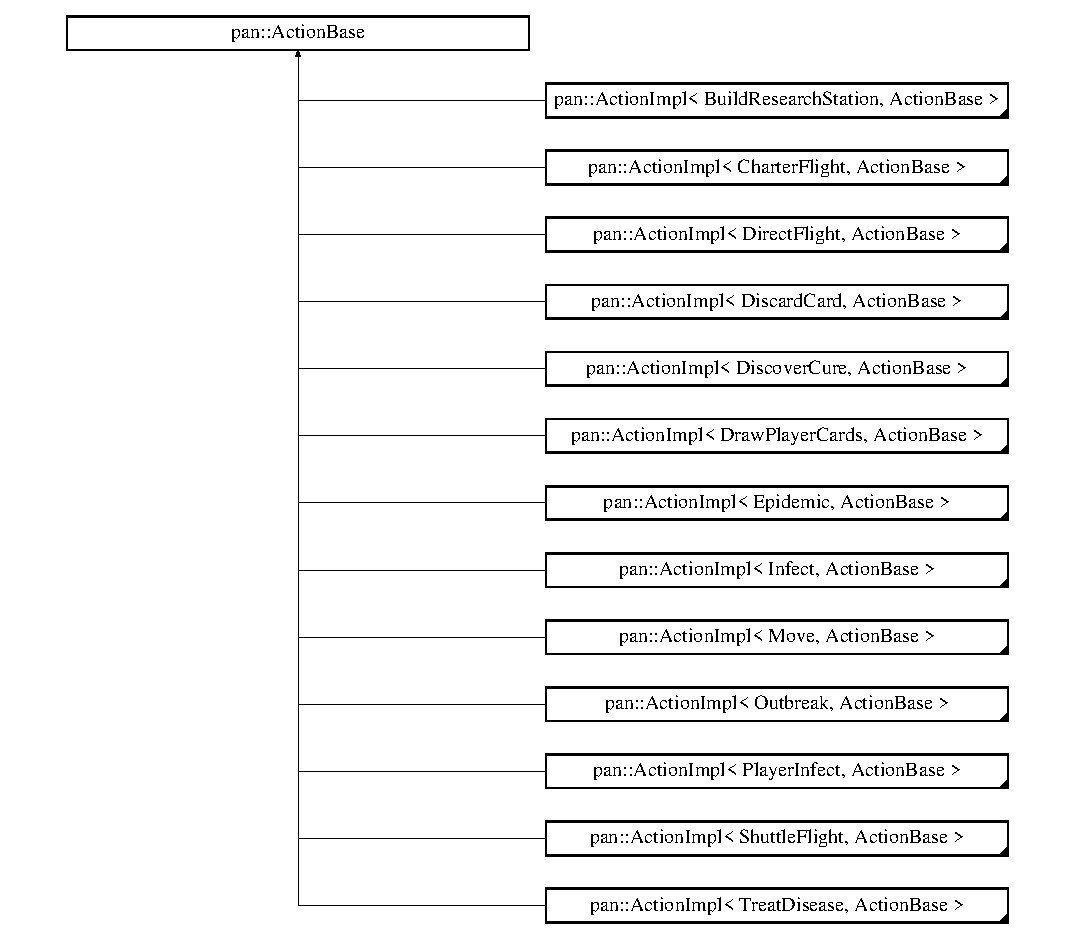
\includegraphics[height=12.000000cm]{classpan_1_1_action_base}
\end{center}
\end{figure}
\subsection*{Public Member Functions}
\begin{DoxyCompactItemize}
\item 
\hyperlink{classpan_1_1_action_base_af413c6b934cf5a26e8fc3af5eebad773}{Action\+Base} ()
\item 
virtual \hyperlink{classpan_1_1_action_base_aac947bf1ed49830f4082727a54989420}{$\sim$\+Action\+Base} ()
\item 
virtual bool \hyperlink{classpan_1_1_action_base_adf042004e303511c8948de5502a59708}{validate} (const \hyperlink{classpan_1_1_action_handler}{Action\+Handler} \&h) const =0
\item 
virtual bool \hyperlink{classpan_1_1_action_base_aba9691736fd1f5ef40a523e988eef6fa}{execute} (\hyperlink{classpan_1_1_action_handler}{Action\+Handler} \&h) const =0
\item 
virtual \hyperlink{classpan_1_1_action_base}{Action\+Base} $\ast$ \hyperlink{classpan_1_1_action_base_a437f541998e59225ab13096a3c8f01c1}{clone} () const =0
\end{DoxyCompactItemize}


\subsection{Detailed Description}
Top level abstraction of the Action entity. Store the Command in the Command pattern. All actions that modify the state of the game, are encapsulated as subclasses of \hyperlink{classpan_1_1_action_base}{Action\+Base}. 

\begin{DoxyAuthor}{Author}
Hrachya Hakobyan 
\end{DoxyAuthor}


\subsection{Constructor \& Destructor Documentation}
\mbox{\Hypertarget{classpan_1_1_action_base_af413c6b934cf5a26e8fc3af5eebad773}\label{classpan_1_1_action_base_af413c6b934cf5a26e8fc3af5eebad773}} 
\index{pan\+::\+Action\+Base@{pan\+::\+Action\+Base}!Action\+Base@{Action\+Base}}
\index{Action\+Base@{Action\+Base}!pan\+::\+Action\+Base@{pan\+::\+Action\+Base}}
\subsubsection{\texorpdfstring{Action\+Base()}{ActionBase()}}
{\footnotesize\ttfamily pan\+::\+Action\+Base\+::\+Action\+Base (\begin{DoxyParamCaption}{ }\end{DoxyParamCaption})\hspace{0.3cm}{\ttfamily [inline]}}

\mbox{\Hypertarget{classpan_1_1_action_base_aac947bf1ed49830f4082727a54989420}\label{classpan_1_1_action_base_aac947bf1ed49830f4082727a54989420}} 
\index{pan\+::\+Action\+Base@{pan\+::\+Action\+Base}!````~Action\+Base@{$\sim$\+Action\+Base}}
\index{````~Action\+Base@{$\sim$\+Action\+Base}!pan\+::\+Action\+Base@{pan\+::\+Action\+Base}}
\subsubsection{\texorpdfstring{$\sim$\+Action\+Base()}{~ActionBase()}}
{\footnotesize\ttfamily virtual pan\+::\+Action\+Base\+::$\sim$\+Action\+Base (\begin{DoxyParamCaption}{ }\end{DoxyParamCaption})\hspace{0.3cm}{\ttfamily [inline]}, {\ttfamily [virtual]}}



\subsection{Member Function Documentation}
\mbox{\Hypertarget{classpan_1_1_action_base_a437f541998e59225ab13096a3c8f01c1}\label{classpan_1_1_action_base_a437f541998e59225ab13096a3c8f01c1}} 
\index{pan\+::\+Action\+Base@{pan\+::\+Action\+Base}!clone@{clone}}
\index{clone@{clone}!pan\+::\+Action\+Base@{pan\+::\+Action\+Base}}
\subsubsection{\texorpdfstring{clone()}{clone()}}
{\footnotesize\ttfamily virtual \hyperlink{classpan_1_1_action_base}{Action\+Base}$\ast$ pan\+::\+Action\+Base\+::clone (\begin{DoxyParamCaption}{ }\end{DoxyParamCaption}) const\hspace{0.3cm}{\ttfamily [pure virtual]}}



Implemented in \hyperlink{classpan_1_1_action_impl_af94569c5a40d1de5c161282000c1a4c7}{pan\+::\+Action\+Impl$<$ Outbreak, Action\+Base $>$}, \hyperlink{classpan_1_1_action_impl_af94569c5a40d1de5c161282000c1a4c7}{pan\+::\+Action\+Impl$<$ Move, Action\+Base $>$}, \hyperlink{classpan_1_1_action_impl_af94569c5a40d1de5c161282000c1a4c7}{pan\+::\+Action\+Impl$<$ Direct\+Flight, Action\+Base $>$}, \hyperlink{classpan_1_1_action_impl_af94569c5a40d1de5c161282000c1a4c7}{pan\+::\+Action\+Impl$<$ Draw\+Player\+Cards, Action\+Base $>$}, \hyperlink{classpan_1_1_action_impl_af94569c5a40d1de5c161282000c1a4c7}{pan\+::\+Action\+Impl$<$ Shuttle\+Flight, Action\+Base $>$}, \hyperlink{classpan_1_1_action_impl_af94569c5a40d1de5c161282000c1a4c7}{pan\+::\+Action\+Impl$<$ Build\+Research\+Station, Action\+Base $>$}, \hyperlink{classpan_1_1_action_impl_af94569c5a40d1de5c161282000c1a4c7}{pan\+::\+Action\+Impl$<$ Treat\+Disease, Action\+Base $>$}, \hyperlink{classpan_1_1_action_impl_af94569c5a40d1de5c161282000c1a4c7}{pan\+::\+Action\+Impl$<$ Player\+Infect, Action\+Base $>$}, \hyperlink{classpan_1_1_action_impl_af94569c5a40d1de5c161282000c1a4c7}{pan\+::\+Action\+Impl$<$ Infect, Action\+Base $>$}, \hyperlink{classpan_1_1_action_impl_af94569c5a40d1de5c161282000c1a4c7}{pan\+::\+Action\+Impl$<$ Epidemic, Action\+Base $>$}, \hyperlink{classpan_1_1_action_impl_af94569c5a40d1de5c161282000c1a4c7}{pan\+::\+Action\+Impl$<$ Discard\+Card, Action\+Base $>$}, \hyperlink{classpan_1_1_action_impl_af94569c5a40d1de5c161282000c1a4c7}{pan\+::\+Action\+Impl$<$ Charter\+Flight, Action\+Base $>$}, and \hyperlink{classpan_1_1_action_impl_af94569c5a40d1de5c161282000c1a4c7}{pan\+::\+Action\+Impl$<$ Discover\+Cure, Action\+Base $>$}.

\mbox{\Hypertarget{classpan_1_1_action_base_aba9691736fd1f5ef40a523e988eef6fa}\label{classpan_1_1_action_base_aba9691736fd1f5ef40a523e988eef6fa}} 
\index{pan\+::\+Action\+Base@{pan\+::\+Action\+Base}!execute@{execute}}
\index{execute@{execute}!pan\+::\+Action\+Base@{pan\+::\+Action\+Base}}
\subsubsection{\texorpdfstring{execute()}{execute()}}
{\footnotesize\ttfamily virtual bool pan\+::\+Action\+Base\+::execute (\begin{DoxyParamCaption}\item[{\hyperlink{classpan_1_1_action_handler}{Action\+Handler} \&}]{h }\end{DoxyParamCaption}) const\hspace{0.3cm}{\ttfamily [pure virtual]}}



Implemented in \hyperlink{classpan_1_1_action_impl_a14d72469bea6d60603d49e4815accb54}{pan\+::\+Action\+Impl$<$ Outbreak, Action\+Base $>$}, \hyperlink{classpan_1_1_action_impl_a14d72469bea6d60603d49e4815accb54}{pan\+::\+Action\+Impl$<$ Move, Action\+Base $>$}, \hyperlink{classpan_1_1_action_impl_a14d72469bea6d60603d49e4815accb54}{pan\+::\+Action\+Impl$<$ Direct\+Flight, Action\+Base $>$}, \hyperlink{classpan_1_1_action_impl_a14d72469bea6d60603d49e4815accb54}{pan\+::\+Action\+Impl$<$ Draw\+Player\+Cards, Action\+Base $>$}, \hyperlink{classpan_1_1_action_impl_a14d72469bea6d60603d49e4815accb54}{pan\+::\+Action\+Impl$<$ Shuttle\+Flight, Action\+Base $>$}, \hyperlink{classpan_1_1_action_impl_a14d72469bea6d60603d49e4815accb54}{pan\+::\+Action\+Impl$<$ Build\+Research\+Station, Action\+Base $>$}, \hyperlink{classpan_1_1_action_impl_a14d72469bea6d60603d49e4815accb54}{pan\+::\+Action\+Impl$<$ Treat\+Disease, Action\+Base $>$}, \hyperlink{classpan_1_1_action_impl_a14d72469bea6d60603d49e4815accb54}{pan\+::\+Action\+Impl$<$ Player\+Infect, Action\+Base $>$}, \hyperlink{classpan_1_1_action_impl_a14d72469bea6d60603d49e4815accb54}{pan\+::\+Action\+Impl$<$ Infect, Action\+Base $>$}, \hyperlink{classpan_1_1_action_impl_a14d72469bea6d60603d49e4815accb54}{pan\+::\+Action\+Impl$<$ Epidemic, Action\+Base $>$}, \hyperlink{classpan_1_1_action_impl_a14d72469bea6d60603d49e4815accb54}{pan\+::\+Action\+Impl$<$ Discard\+Card, Action\+Base $>$}, \hyperlink{classpan_1_1_action_impl_a14d72469bea6d60603d49e4815accb54}{pan\+::\+Action\+Impl$<$ Charter\+Flight, Action\+Base $>$}, and \hyperlink{classpan_1_1_action_impl_a14d72469bea6d60603d49e4815accb54}{pan\+::\+Action\+Impl$<$ Discover\+Cure, Action\+Base $>$}.

\mbox{\Hypertarget{classpan_1_1_action_base_adf042004e303511c8948de5502a59708}\label{classpan_1_1_action_base_adf042004e303511c8948de5502a59708}} 
\index{pan\+::\+Action\+Base@{pan\+::\+Action\+Base}!validate@{validate}}
\index{validate@{validate}!pan\+::\+Action\+Base@{pan\+::\+Action\+Base}}
\subsubsection{\texorpdfstring{validate()}{validate()}}
{\footnotesize\ttfamily virtual bool pan\+::\+Action\+Base\+::validate (\begin{DoxyParamCaption}\item[{const \hyperlink{classpan_1_1_action_handler}{Action\+Handler} \&}]{h }\end{DoxyParamCaption}) const\hspace{0.3cm}{\ttfamily [pure virtual]}}



Implemented in \hyperlink{classpan_1_1_action_impl_acea764a5b41d2fd21717089e21d0c6f4}{pan\+::\+Action\+Impl$<$ Outbreak, Action\+Base $>$}, \hyperlink{classpan_1_1_action_impl_acea764a5b41d2fd21717089e21d0c6f4}{pan\+::\+Action\+Impl$<$ Move, Action\+Base $>$}, \hyperlink{classpan_1_1_action_impl_acea764a5b41d2fd21717089e21d0c6f4}{pan\+::\+Action\+Impl$<$ Direct\+Flight, Action\+Base $>$}, \hyperlink{classpan_1_1_action_impl_acea764a5b41d2fd21717089e21d0c6f4}{pan\+::\+Action\+Impl$<$ Draw\+Player\+Cards, Action\+Base $>$}, \hyperlink{classpan_1_1_action_impl_acea764a5b41d2fd21717089e21d0c6f4}{pan\+::\+Action\+Impl$<$ Shuttle\+Flight, Action\+Base $>$}, \hyperlink{classpan_1_1_action_impl_acea764a5b41d2fd21717089e21d0c6f4}{pan\+::\+Action\+Impl$<$ Build\+Research\+Station, Action\+Base $>$}, \hyperlink{classpan_1_1_action_impl_acea764a5b41d2fd21717089e21d0c6f4}{pan\+::\+Action\+Impl$<$ Treat\+Disease, Action\+Base $>$}, \hyperlink{classpan_1_1_action_impl_acea764a5b41d2fd21717089e21d0c6f4}{pan\+::\+Action\+Impl$<$ Player\+Infect, Action\+Base $>$}, \hyperlink{classpan_1_1_action_impl_acea764a5b41d2fd21717089e21d0c6f4}{pan\+::\+Action\+Impl$<$ Infect, Action\+Base $>$}, \hyperlink{classpan_1_1_action_impl_acea764a5b41d2fd21717089e21d0c6f4}{pan\+::\+Action\+Impl$<$ Epidemic, Action\+Base $>$}, \hyperlink{classpan_1_1_action_impl_acea764a5b41d2fd21717089e21d0c6f4}{pan\+::\+Action\+Impl$<$ Discard\+Card, Action\+Base $>$}, \hyperlink{classpan_1_1_action_impl_acea764a5b41d2fd21717089e21d0c6f4}{pan\+::\+Action\+Impl$<$ Charter\+Flight, Action\+Base $>$}, and \hyperlink{classpan_1_1_action_impl_acea764a5b41d2fd21717089e21d0c6f4}{pan\+::\+Action\+Impl$<$ Discover\+Cure, Action\+Base $>$}.



The documentation for this class was generated from the following file\+:\begin{DoxyCompactItemize}
\item 
\hyperlink{_action_base_8h}{Action\+Base.\+h}\end{DoxyCompactItemize}

\hypertarget{classpan_1_1_action_handler}{}\section{pan\+:\+:Action\+Handler Class Reference}
\label{classpan_1_1_action_handler}\index{pan\+::\+Action\+Handler@{pan\+::\+Action\+Handler}}


Class containing the logic of validating and executing actions. Directly connected to a \hyperlink{classpan_1_1_game}{Game} object through a reference. Does not store any state, is free from serialization.  




{\ttfamily \#include $<$Action\+Handler.\+h$>$}

\subsection*{Public Member Functions}
\begin{DoxyCompactItemize}
\item 
\hyperlink{classpan_1_1_action_handler_a5aeb269dae11a6bd190fafd945a508a1}{Action\+Handler} (\hyperlink{classpan_1_1_game}{Game} \&game)
\item 
\hyperlink{classpan_1_1_action_handler_a56b3a54ca19b9d071adffa0a9ac7b266}{Action\+Handler} ()=delete
\item 
\hyperlink{classpan_1_1_action_handler_a403ff5c81573b682a5dfc9d476be8e4e}{Action\+Handler} (const \hyperlink{classpan_1_1_action_handler}{Action\+Handler} \&)=delete
\item 
\hyperlink{classpan_1_1_action_handler_a5bf64631c974765b04def48c0df0fcd7}{$\sim$\+Action\+Handler} ()
\item 
{\footnotesize template$<$typename Action $>$ }\\bool \hyperlink{classpan_1_1_action_handler_ae2a8bd5ae0560677aeafe7b6c068adb7}{validate} (const Action \&action) const
\item 
{\footnotesize template$<$typename Action $>$ }\\bool \hyperlink{classpan_1_1_action_handler_a7c5cefcd45fe538da04762de3cac0dbd}{execute} (const Action \&action)
\item 
{\footnotesize template$<$$>$ }\\bool \hyperlink{classpan_1_1_action_handler_a3e2fc1b454ace0dd42b3b4bacc22eb0d}{validate} (const \hyperlink{classpan_1_1_move}{Move} \&m) const
\item 
{\footnotesize template$<$$>$ }\\bool \hyperlink{classpan_1_1_action_handler_a97f0f5801dedcbc42396f185686083bb}{execute} (const \hyperlink{classpan_1_1_move}{Move} \&m)
\item 
{\footnotesize template$<$$>$ }\\bool \hyperlink{classpan_1_1_action_handler_aa3788249f03ad2eaa4cdaf375b7da3d2}{validate} (const \hyperlink{classpan_1_1_direct_flight}{Direct\+Flight} \&m) const
\item 
{\footnotesize template$<$$>$ }\\bool \hyperlink{classpan_1_1_action_handler_ad72cd3c55d494ca5941e1b9f46e6d6b7}{execute} (const \hyperlink{classpan_1_1_direct_flight}{Direct\+Flight} \&m)
\item 
{\footnotesize template$<$$>$ }\\bool \hyperlink{classpan_1_1_action_handler_a6eade14ec30fec3d40adf7b3ddbf1ed5}{validate} (const \hyperlink{classpan_1_1_charter_flight}{Charter\+Flight} \&m) const
\item 
{\footnotesize template$<$$>$ }\\bool \hyperlink{classpan_1_1_action_handler_a2f471e252e4cff4e06e9f95309f2049a}{execute} (const \hyperlink{classpan_1_1_charter_flight}{Charter\+Flight} \&m)
\item 
{\footnotesize template$<$$>$ }\\bool \hyperlink{classpan_1_1_action_handler_a3b8964b9b1888df96c71da3447967656}{validate} (const \hyperlink{classpan_1_1_shuttle_flight}{Shuttle\+Flight} \&m) const
\item 
{\footnotesize template$<$$>$ }\\bool \hyperlink{classpan_1_1_action_handler_ae5962fc9522e37b575fe9922cb28e040}{execute} (const \hyperlink{classpan_1_1_shuttle_flight}{Shuttle\+Flight} \&m)
\item 
{\footnotesize template$<$$>$ }\\bool \hyperlink{classpan_1_1_action_handler_ad55077a791011a4af860f67793d0e3e5}{validate} (const \hyperlink{classpan_1_1_build_research_station}{Build\+Research\+Station} \&m) const
\item 
{\footnotesize template$<$$>$ }\\bool \hyperlink{classpan_1_1_action_handler_a82301269ae5559636bdd1e41373757d6}{execute} (const \hyperlink{classpan_1_1_build_research_station}{Build\+Research\+Station} \&m)
\item 
{\footnotesize template$<$$>$ }\\bool \hyperlink{classpan_1_1_action_handler_a9d0117592a8ef88cbb945e82b0676f58}{validate} (const \hyperlink{classpan_1_1_treat_disease}{Treat\+Disease} \&m) const
\item 
{\footnotesize template$<$$>$ }\\bool \hyperlink{classpan_1_1_action_handler_adcbd9a954dcbaa6b968facd6395797a6}{execute} (const \hyperlink{classpan_1_1_treat_disease}{Treat\+Disease} \&m)
\item 
{\footnotesize template$<$$>$ }\\bool \hyperlink{classpan_1_1_action_handler_a148408970391d77cc793b5e33fe55789}{validate} (const \hyperlink{classpan_1_1_discover_cure}{Discover\+Cure} \&m) const
\begin{DoxyCompactList}\small\item\em validates the discover cure action The action is valid if the following hold \end{DoxyCompactList}\item 
{\footnotesize template$<$$>$ }\\bool \hyperlink{classpan_1_1_action_handler_aa39cbd76ffdebb15c21890730a79606d}{execute} (const \hyperlink{classpan_1_1_discover_cure}{Discover\+Cure} \&m)
\item 
{\footnotesize template$<$$>$ }\\bool \hyperlink{classpan_1_1_action_handler_a6e4ee30f39708e81fa435d13d3b27919}{validate} (const \hyperlink{classpan_1_1_draw_player_cards}{Draw\+Player\+Cards} \&a) const
\begin{DoxyCompactList}\small\item\em validates Drawplayer\+Cards action the action is valid if the following hold \end{DoxyCompactList}\item 
{\footnotesize template$<$$>$ }\\bool \hyperlink{classpan_1_1_action_handler_a1dbb4c4c6404625a9660d1d5f7b94dc5}{execute} (const \hyperlink{classpan_1_1_draw_player_cards}{Draw\+Player\+Cards} \&a)
\item 
{\footnotesize template$<$$>$ }\\bool \hyperlink{classpan_1_1_action_handler_af6d6407b345efff7c1d2ecb50a0af563}{validate} (const \hyperlink{classpan_1_1_player_infect}{Player\+Infect} \&a) const
\begin{DoxyCompactList}\small\item\em validates \hyperlink{classpan_1_1_player_infect}{Player\+Infect} action The action is valid if the following hold. \end{DoxyCompactList}\item 
{\footnotesize template$<$$>$ }\\bool \hyperlink{classpan_1_1_action_handler_a1ebea9d9a8bb894945e1ad0ecc7821c9}{execute} (const \hyperlink{classpan_1_1_player_infect}{Player\+Infect} \&a)
\item 
{\footnotesize template$<$$>$ }\\bool \hyperlink{classpan_1_1_action_handler_af6175819ceeba99896279c04401a5393}{validate} (const \hyperlink{classpan_1_1_discard_card}{Discard\+Card} \&a) const
\begin{DoxyCompactList}\small\item\em validates \hyperlink{classpan_1_1_discard_card}{Discard\+Card} action The action is valid if the following hold. \end{DoxyCompactList}\item 
{\footnotesize template$<$$>$ }\\bool \hyperlink{classpan_1_1_action_handler_a829a5d84e0fd082391be32ed3a680ae4}{execute} (const \hyperlink{classpan_1_1_discard_card}{Discard\+Card} \&a)
\item 
{\footnotesize template$<$$>$ }\\bool \hyperlink{classpan_1_1_action_handler_a628fc9ae167c2d421644a12e93b8137c}{validate} (const \hyperlink{classpan_1_1_outbreak}{Outbreak} \&a) const
\item 
{\footnotesize template$<$$>$ }\\bool \hyperlink{classpan_1_1_action_handler_ad2119c276b50e56a42553671fc6e1e70}{execute} (const \hyperlink{classpan_1_1_outbreak}{Outbreak} \&a)
\item 
{\footnotesize template$<$$>$ }\\bool \hyperlink{classpan_1_1_action_handler_a0dc0214533aeb931e6c119e15caaee6a}{validate} (const \hyperlink{classpan_1_1_infect}{Infect} \&a) const
\item 
{\footnotesize template$<$$>$ }\\bool \hyperlink{classpan_1_1_action_handler_ade755aaadb764489a68634811314bee2}{execute} (const \hyperlink{classpan_1_1_infect}{Infect} \&a)
\item 
{\footnotesize template$<$$>$ }\\bool \hyperlink{classpan_1_1_action_handler_a28ed770b339cba18d970a153c82d3c45}{validate} (const \hyperlink{classpan_1_1_epidemic}{Epidemic} \&a) const
\item 
{\footnotesize template$<$$>$ }\\bool \hyperlink{classpan_1_1_action_handler_a469f04bd874aca38c9b3792aee209703}{execute} (const \hyperlink{classpan_1_1_epidemic}{Epidemic} \&a)
\end{DoxyCompactItemize}


\subsection{Detailed Description}
Class containing the logic of validating and executing actions. Directly connected to a \hyperlink{classpan_1_1_game}{Game} object through a reference. Does not store any state, is free from serialization. 

\begin{DoxyAuthor}{Author}
Hrachya Hakobyan 
\end{DoxyAuthor}


\subsection{Constructor \& Destructor Documentation}
\mbox{\Hypertarget{classpan_1_1_action_handler_a5aeb269dae11a6bd190fafd945a508a1}\label{classpan_1_1_action_handler_a5aeb269dae11a6bd190fafd945a508a1}} 
\index{pan\+::\+Action\+Handler@{pan\+::\+Action\+Handler}!Action\+Handler@{Action\+Handler}}
\index{Action\+Handler@{Action\+Handler}!pan\+::\+Action\+Handler@{pan\+::\+Action\+Handler}}
\subsubsection{\texorpdfstring{Action\+Handler()}{ActionHandler()}\hspace{0.1cm}{\footnotesize\ttfamily [1/3]}}
{\footnotesize\ttfamily pan\+::\+Action\+Handler\+::\+Action\+Handler (\begin{DoxyParamCaption}\item[{\hyperlink{classpan_1_1_game}{Game} \&}]{game }\end{DoxyParamCaption})\hspace{0.3cm}{\ttfamily [explicit]}}

\mbox{\Hypertarget{classpan_1_1_action_handler_a56b3a54ca19b9d071adffa0a9ac7b266}\label{classpan_1_1_action_handler_a56b3a54ca19b9d071adffa0a9ac7b266}} 
\index{pan\+::\+Action\+Handler@{pan\+::\+Action\+Handler}!Action\+Handler@{Action\+Handler}}
\index{Action\+Handler@{Action\+Handler}!pan\+::\+Action\+Handler@{pan\+::\+Action\+Handler}}
\subsubsection{\texorpdfstring{Action\+Handler()}{ActionHandler()}\hspace{0.1cm}{\footnotesize\ttfamily [2/3]}}
{\footnotesize\ttfamily pan\+::\+Action\+Handler\+::\+Action\+Handler (\begin{DoxyParamCaption}{ }\end{DoxyParamCaption})\hspace{0.3cm}{\ttfamily [delete]}}

\mbox{\Hypertarget{classpan_1_1_action_handler_a403ff5c81573b682a5dfc9d476be8e4e}\label{classpan_1_1_action_handler_a403ff5c81573b682a5dfc9d476be8e4e}} 
\index{pan\+::\+Action\+Handler@{pan\+::\+Action\+Handler}!Action\+Handler@{Action\+Handler}}
\index{Action\+Handler@{Action\+Handler}!pan\+::\+Action\+Handler@{pan\+::\+Action\+Handler}}
\subsubsection{\texorpdfstring{Action\+Handler()}{ActionHandler()}\hspace{0.1cm}{\footnotesize\ttfamily [3/3]}}
{\footnotesize\ttfamily pan\+::\+Action\+Handler\+::\+Action\+Handler (\begin{DoxyParamCaption}\item[{const \hyperlink{classpan_1_1_action_handler}{Action\+Handler} \&}]{ }\end{DoxyParamCaption})\hspace{0.3cm}{\ttfamily [delete]}}

\mbox{\Hypertarget{classpan_1_1_action_handler_a5bf64631c974765b04def48c0df0fcd7}\label{classpan_1_1_action_handler_a5bf64631c974765b04def48c0df0fcd7}} 
\index{pan\+::\+Action\+Handler@{pan\+::\+Action\+Handler}!````~Action\+Handler@{$\sim$\+Action\+Handler}}
\index{````~Action\+Handler@{$\sim$\+Action\+Handler}!pan\+::\+Action\+Handler@{pan\+::\+Action\+Handler}}
\subsubsection{\texorpdfstring{$\sim$\+Action\+Handler()}{~ActionHandler()}}
{\footnotesize\ttfamily pan\+::\+Action\+Handler\+::$\sim$\+Action\+Handler (\begin{DoxyParamCaption}{ }\end{DoxyParamCaption})}



\subsection{Member Function Documentation}
\mbox{\Hypertarget{classpan_1_1_action_handler_a7c5cefcd45fe538da04762de3cac0dbd}\label{classpan_1_1_action_handler_a7c5cefcd45fe538da04762de3cac0dbd}} 
\index{pan\+::\+Action\+Handler@{pan\+::\+Action\+Handler}!execute@{execute}}
\index{execute@{execute}!pan\+::\+Action\+Handler@{pan\+::\+Action\+Handler}}
\subsubsection{\texorpdfstring{execute()}{execute()}\hspace{0.1cm}{\footnotesize\ttfamily [1/14]}}
{\footnotesize\ttfamily template$<$typename Action $>$ \\
bool pan\+::\+Action\+Handler\+::execute (\begin{DoxyParamCaption}\item[{const Action \&}]{action }\end{DoxyParamCaption})}

Executes the given action. The action is validated before execution. A valid action will always execute. 
\begin{DoxyParams}{Parameters}
{\em action} & a subclass of \hyperlink{classpan_1_1_action_impl}{Action\+Impl} \\
\hline
\end{DoxyParams}
\begin{DoxyReturn}{Returns}
true if the action was valid, false otherwise 
\end{DoxyReturn}
\mbox{\Hypertarget{classpan_1_1_action_handler_a97f0f5801dedcbc42396f185686083bb}\label{classpan_1_1_action_handler_a97f0f5801dedcbc42396f185686083bb}} 
\index{pan\+::\+Action\+Handler@{pan\+::\+Action\+Handler}!execute@{execute}}
\index{execute@{execute}!pan\+::\+Action\+Handler@{pan\+::\+Action\+Handler}}
\subsubsection{\texorpdfstring{execute()}{execute()}\hspace{0.1cm}{\footnotesize\ttfamily [2/14]}}
{\footnotesize\ttfamily template$<$$>$ \\
bool pan\+::\+Action\+Handler\+::execute (\begin{DoxyParamCaption}\item[{const \hyperlink{classpan_1_1_move}{Move} \&}]{m }\end{DoxyParamCaption})}

\mbox{\Hypertarget{classpan_1_1_action_handler_ad72cd3c55d494ca5941e1b9f46e6d6b7}\label{classpan_1_1_action_handler_ad72cd3c55d494ca5941e1b9f46e6d6b7}} 
\index{pan\+::\+Action\+Handler@{pan\+::\+Action\+Handler}!execute@{execute}}
\index{execute@{execute}!pan\+::\+Action\+Handler@{pan\+::\+Action\+Handler}}
\subsubsection{\texorpdfstring{execute()}{execute()}\hspace{0.1cm}{\footnotesize\ttfamily [3/14]}}
{\footnotesize\ttfamily template$<$$>$ \\
bool pan\+::\+Action\+Handler\+::execute (\begin{DoxyParamCaption}\item[{const \hyperlink{classpan_1_1_direct_flight}{Direct\+Flight} \&}]{m }\end{DoxyParamCaption})}

\mbox{\Hypertarget{classpan_1_1_action_handler_a2f471e252e4cff4e06e9f95309f2049a}\label{classpan_1_1_action_handler_a2f471e252e4cff4e06e9f95309f2049a}} 
\index{pan\+::\+Action\+Handler@{pan\+::\+Action\+Handler}!execute@{execute}}
\index{execute@{execute}!pan\+::\+Action\+Handler@{pan\+::\+Action\+Handler}}
\subsubsection{\texorpdfstring{execute()}{execute()}\hspace{0.1cm}{\footnotesize\ttfamily [4/14]}}
{\footnotesize\ttfamily template$<$$>$ \\
bool pan\+::\+Action\+Handler\+::execute (\begin{DoxyParamCaption}\item[{const \hyperlink{classpan_1_1_charter_flight}{Charter\+Flight} \&}]{m }\end{DoxyParamCaption})}

\mbox{\Hypertarget{classpan_1_1_action_handler_ae5962fc9522e37b575fe9922cb28e040}\label{classpan_1_1_action_handler_ae5962fc9522e37b575fe9922cb28e040}} 
\index{pan\+::\+Action\+Handler@{pan\+::\+Action\+Handler}!execute@{execute}}
\index{execute@{execute}!pan\+::\+Action\+Handler@{pan\+::\+Action\+Handler}}
\subsubsection{\texorpdfstring{execute()}{execute()}\hspace{0.1cm}{\footnotesize\ttfamily [5/14]}}
{\footnotesize\ttfamily template$<$$>$ \\
bool pan\+::\+Action\+Handler\+::execute (\begin{DoxyParamCaption}\item[{const \hyperlink{classpan_1_1_shuttle_flight}{Shuttle\+Flight} \&}]{m }\end{DoxyParamCaption})}

\mbox{\Hypertarget{classpan_1_1_action_handler_a82301269ae5559636bdd1e41373757d6}\label{classpan_1_1_action_handler_a82301269ae5559636bdd1e41373757d6}} 
\index{pan\+::\+Action\+Handler@{pan\+::\+Action\+Handler}!execute@{execute}}
\index{execute@{execute}!pan\+::\+Action\+Handler@{pan\+::\+Action\+Handler}}
\subsubsection{\texorpdfstring{execute()}{execute()}\hspace{0.1cm}{\footnotesize\ttfamily [6/14]}}
{\footnotesize\ttfamily template$<$$>$ \\
bool pan\+::\+Action\+Handler\+::execute (\begin{DoxyParamCaption}\item[{const \hyperlink{classpan_1_1_build_research_station}{Build\+Research\+Station} \&}]{m }\end{DoxyParamCaption})}

\mbox{\Hypertarget{classpan_1_1_action_handler_adcbd9a954dcbaa6b968facd6395797a6}\label{classpan_1_1_action_handler_adcbd9a954dcbaa6b968facd6395797a6}} 
\index{pan\+::\+Action\+Handler@{pan\+::\+Action\+Handler}!execute@{execute}}
\index{execute@{execute}!pan\+::\+Action\+Handler@{pan\+::\+Action\+Handler}}
\subsubsection{\texorpdfstring{execute()}{execute()}\hspace{0.1cm}{\footnotesize\ttfamily [7/14]}}
{\footnotesize\ttfamily template$<$$>$ \\
bool pan\+::\+Action\+Handler\+::execute (\begin{DoxyParamCaption}\item[{const \hyperlink{classpan_1_1_treat_disease}{Treat\+Disease} \&}]{m }\end{DoxyParamCaption})}

\mbox{\Hypertarget{classpan_1_1_action_handler_aa39cbd76ffdebb15c21890730a79606d}\label{classpan_1_1_action_handler_aa39cbd76ffdebb15c21890730a79606d}} 
\index{pan\+::\+Action\+Handler@{pan\+::\+Action\+Handler}!execute@{execute}}
\index{execute@{execute}!pan\+::\+Action\+Handler@{pan\+::\+Action\+Handler}}
\subsubsection{\texorpdfstring{execute()}{execute()}\hspace{0.1cm}{\footnotesize\ttfamily [8/14]}}
{\footnotesize\ttfamily template$<$$>$ \\
bool pan\+::\+Action\+Handler\+::execute (\begin{DoxyParamCaption}\item[{const \hyperlink{classpan_1_1_discover_cure}{Discover\+Cure} \&}]{m }\end{DoxyParamCaption})}

\mbox{\Hypertarget{classpan_1_1_action_handler_a1dbb4c4c6404625a9660d1d5f7b94dc5}\label{classpan_1_1_action_handler_a1dbb4c4c6404625a9660d1d5f7b94dc5}} 
\index{pan\+::\+Action\+Handler@{pan\+::\+Action\+Handler}!execute@{execute}}
\index{execute@{execute}!pan\+::\+Action\+Handler@{pan\+::\+Action\+Handler}}
\subsubsection{\texorpdfstring{execute()}{execute()}\hspace{0.1cm}{\footnotesize\ttfamily [9/14]}}
{\footnotesize\ttfamily template$<$$>$ \\
bool pan\+::\+Action\+Handler\+::execute (\begin{DoxyParamCaption}\item[{const \hyperlink{classpan_1_1_draw_player_cards}{Draw\+Player\+Cards} \&}]{a }\end{DoxyParamCaption})}

\mbox{\Hypertarget{classpan_1_1_action_handler_a1ebea9d9a8bb894945e1ad0ecc7821c9}\label{classpan_1_1_action_handler_a1ebea9d9a8bb894945e1ad0ecc7821c9}} 
\index{pan\+::\+Action\+Handler@{pan\+::\+Action\+Handler}!execute@{execute}}
\index{execute@{execute}!pan\+::\+Action\+Handler@{pan\+::\+Action\+Handler}}
\subsubsection{\texorpdfstring{execute()}{execute()}\hspace{0.1cm}{\footnotesize\ttfamily [10/14]}}
{\footnotesize\ttfamily template$<$$>$ \\
bool pan\+::\+Action\+Handler\+::execute (\begin{DoxyParamCaption}\item[{const \hyperlink{classpan_1_1_player_infect}{Player\+Infect} \&}]{a }\end{DoxyParamCaption})}

\mbox{\Hypertarget{classpan_1_1_action_handler_a829a5d84e0fd082391be32ed3a680ae4}\label{classpan_1_1_action_handler_a829a5d84e0fd082391be32ed3a680ae4}} 
\index{pan\+::\+Action\+Handler@{pan\+::\+Action\+Handler}!execute@{execute}}
\index{execute@{execute}!pan\+::\+Action\+Handler@{pan\+::\+Action\+Handler}}
\subsubsection{\texorpdfstring{execute()}{execute()}\hspace{0.1cm}{\footnotesize\ttfamily [11/14]}}
{\footnotesize\ttfamily template$<$$>$ \\
bool pan\+::\+Action\+Handler\+::execute (\begin{DoxyParamCaption}\item[{const \hyperlink{classpan_1_1_discard_card}{Discard\+Card} \&}]{a }\end{DoxyParamCaption})}

\mbox{\Hypertarget{classpan_1_1_action_handler_ad2119c276b50e56a42553671fc6e1e70}\label{classpan_1_1_action_handler_ad2119c276b50e56a42553671fc6e1e70}} 
\index{pan\+::\+Action\+Handler@{pan\+::\+Action\+Handler}!execute@{execute}}
\index{execute@{execute}!pan\+::\+Action\+Handler@{pan\+::\+Action\+Handler}}
\subsubsection{\texorpdfstring{execute()}{execute()}\hspace{0.1cm}{\footnotesize\ttfamily [12/14]}}
{\footnotesize\ttfamily template$<$$>$ \\
bool pan\+::\+Action\+Handler\+::execute (\begin{DoxyParamCaption}\item[{const \hyperlink{classpan_1_1_outbreak}{Outbreak} \&}]{a }\end{DoxyParamCaption})}

\mbox{\Hypertarget{classpan_1_1_action_handler_ade755aaadb764489a68634811314bee2}\label{classpan_1_1_action_handler_ade755aaadb764489a68634811314bee2}} 
\index{pan\+::\+Action\+Handler@{pan\+::\+Action\+Handler}!execute@{execute}}
\index{execute@{execute}!pan\+::\+Action\+Handler@{pan\+::\+Action\+Handler}}
\subsubsection{\texorpdfstring{execute()}{execute()}\hspace{0.1cm}{\footnotesize\ttfamily [13/14]}}
{\footnotesize\ttfamily template$<$$>$ \\
bool pan\+::\+Action\+Handler\+::execute (\begin{DoxyParamCaption}\item[{const \hyperlink{classpan_1_1_infect}{Infect} \&}]{a }\end{DoxyParamCaption})}

\mbox{\Hypertarget{classpan_1_1_action_handler_a469f04bd874aca38c9b3792aee209703}\label{classpan_1_1_action_handler_a469f04bd874aca38c9b3792aee209703}} 
\index{pan\+::\+Action\+Handler@{pan\+::\+Action\+Handler}!execute@{execute}}
\index{execute@{execute}!pan\+::\+Action\+Handler@{pan\+::\+Action\+Handler}}
\subsubsection{\texorpdfstring{execute()}{execute()}\hspace{0.1cm}{\footnotesize\ttfamily [14/14]}}
{\footnotesize\ttfamily template$<$$>$ \\
bool pan\+::\+Action\+Handler\+::execute (\begin{DoxyParamCaption}\item[{const \hyperlink{classpan_1_1_epidemic}{Epidemic} \&}]{a }\end{DoxyParamCaption})}

\mbox{\Hypertarget{classpan_1_1_action_handler_ae2a8bd5ae0560677aeafe7b6c068adb7}\label{classpan_1_1_action_handler_ae2a8bd5ae0560677aeafe7b6c068adb7}} 
\index{pan\+::\+Action\+Handler@{pan\+::\+Action\+Handler}!validate@{validate}}
\index{validate@{validate}!pan\+::\+Action\+Handler@{pan\+::\+Action\+Handler}}
\subsubsection{\texorpdfstring{validate()}{validate()}\hspace{0.1cm}{\footnotesize\ttfamily [1/14]}}
{\footnotesize\ttfamily template$<$typename Action $>$ \\
bool pan\+::\+Action\+Handler\+::validate (\begin{DoxyParamCaption}\item[{const Action \&}]{action }\end{DoxyParamCaption}) const}

Validates the given action 
\begin{DoxyParams}{Parameters}
{\em action} & a subclass of \hyperlink{classpan_1_1_action_impl}{Action\+Impl} \\
\hline
\end{DoxyParams}
\begin{DoxyReturn}{Returns}
true if the action is valid, false otherwise 
\end{DoxyReturn}
\mbox{\Hypertarget{classpan_1_1_action_handler_a3e2fc1b454ace0dd42b3b4bacc22eb0d}\label{classpan_1_1_action_handler_a3e2fc1b454ace0dd42b3b4bacc22eb0d}} 
\index{pan\+::\+Action\+Handler@{pan\+::\+Action\+Handler}!validate@{validate}}
\index{validate@{validate}!pan\+::\+Action\+Handler@{pan\+::\+Action\+Handler}}
\subsubsection{\texorpdfstring{validate()}{validate()}\hspace{0.1cm}{\footnotesize\ttfamily [2/14]}}
{\footnotesize\ttfamily template$<$$>$ \\
bool pan\+::\+Action\+Handler\+::validate (\begin{DoxyParamCaption}\item[{const \hyperlink{classpan_1_1_move}{Move} \&}]{m }\end{DoxyParamCaption}) const}

Validates \hyperlink{classpan_1_1_move}{Move} action. A move action is valid if the following hold 1.\+The player exists.
\begin{DoxyEnumerate}
\item It is the player\textquotesingle{}s turn.
\item The player can make an action.
\item The target city is not the same as the player\textquotesingle{}s city.
\item The target city is a neighbor of the player\textquotesingle{}s city. 
\end{DoxyEnumerate}\mbox{\Hypertarget{classpan_1_1_action_handler_aa3788249f03ad2eaa4cdaf375b7da3d2}\label{classpan_1_1_action_handler_aa3788249f03ad2eaa4cdaf375b7da3d2}} 
\index{pan\+::\+Action\+Handler@{pan\+::\+Action\+Handler}!validate@{validate}}
\index{validate@{validate}!pan\+::\+Action\+Handler@{pan\+::\+Action\+Handler}}
\subsubsection{\texorpdfstring{validate()}{validate()}\hspace{0.1cm}{\footnotesize\ttfamily [3/14]}}
{\footnotesize\ttfamily template$<$$>$ \\
bool pan\+::\+Action\+Handler\+::validate (\begin{DoxyParamCaption}\item[{const \hyperlink{classpan_1_1_direct_flight}{Direct\+Flight} \&}]{m }\end{DoxyParamCaption}) const}

\mbox{\Hypertarget{classpan_1_1_action_handler_a6eade14ec30fec3d40adf7b3ddbf1ed5}\label{classpan_1_1_action_handler_a6eade14ec30fec3d40adf7b3ddbf1ed5}} 
\index{pan\+::\+Action\+Handler@{pan\+::\+Action\+Handler}!validate@{validate}}
\index{validate@{validate}!pan\+::\+Action\+Handler@{pan\+::\+Action\+Handler}}
\subsubsection{\texorpdfstring{validate()}{validate()}\hspace{0.1cm}{\footnotesize\ttfamily [4/14]}}
{\footnotesize\ttfamily template$<$$>$ \\
bool pan\+::\+Action\+Handler\+::validate (\begin{DoxyParamCaption}\item[{const \hyperlink{classpan_1_1_charter_flight}{Charter\+Flight} \&}]{m }\end{DoxyParamCaption}) const}

\mbox{\Hypertarget{classpan_1_1_action_handler_a3b8964b9b1888df96c71da3447967656}\label{classpan_1_1_action_handler_a3b8964b9b1888df96c71da3447967656}} 
\index{pan\+::\+Action\+Handler@{pan\+::\+Action\+Handler}!validate@{validate}}
\index{validate@{validate}!pan\+::\+Action\+Handler@{pan\+::\+Action\+Handler}}
\subsubsection{\texorpdfstring{validate()}{validate()}\hspace{0.1cm}{\footnotesize\ttfamily [5/14]}}
{\footnotesize\ttfamily template$<$$>$ \\
bool pan\+::\+Action\+Handler\+::validate (\begin{DoxyParamCaption}\item[{const \hyperlink{classpan_1_1_shuttle_flight}{Shuttle\+Flight} \&}]{m }\end{DoxyParamCaption}) const}

\mbox{\Hypertarget{classpan_1_1_action_handler_ad55077a791011a4af860f67793d0e3e5}\label{classpan_1_1_action_handler_ad55077a791011a4af860f67793d0e3e5}} 
\index{pan\+::\+Action\+Handler@{pan\+::\+Action\+Handler}!validate@{validate}}
\index{validate@{validate}!pan\+::\+Action\+Handler@{pan\+::\+Action\+Handler}}
\subsubsection{\texorpdfstring{validate()}{validate()}\hspace{0.1cm}{\footnotesize\ttfamily [6/14]}}
{\footnotesize\ttfamily template$<$$>$ \\
bool pan\+::\+Action\+Handler\+::validate (\begin{DoxyParamCaption}\item[{const \hyperlink{classpan_1_1_build_research_station}{Build\+Research\+Station} \&}]{m }\end{DoxyParamCaption}) const}

\mbox{\Hypertarget{classpan_1_1_action_handler_a9d0117592a8ef88cbb945e82b0676f58}\label{classpan_1_1_action_handler_a9d0117592a8ef88cbb945e82b0676f58}} 
\index{pan\+::\+Action\+Handler@{pan\+::\+Action\+Handler}!validate@{validate}}
\index{validate@{validate}!pan\+::\+Action\+Handler@{pan\+::\+Action\+Handler}}
\subsubsection{\texorpdfstring{validate()}{validate()}\hspace{0.1cm}{\footnotesize\ttfamily [7/14]}}
{\footnotesize\ttfamily template$<$$>$ \\
bool pan\+::\+Action\+Handler\+::validate (\begin{DoxyParamCaption}\item[{const \hyperlink{classpan_1_1_treat_disease}{Treat\+Disease} \&}]{m }\end{DoxyParamCaption}) const}

\mbox{\Hypertarget{classpan_1_1_action_handler_a148408970391d77cc793b5e33fe55789}\label{classpan_1_1_action_handler_a148408970391d77cc793b5e33fe55789}} 
\index{pan\+::\+Action\+Handler@{pan\+::\+Action\+Handler}!validate@{validate}}
\index{validate@{validate}!pan\+::\+Action\+Handler@{pan\+::\+Action\+Handler}}
\subsubsection{\texorpdfstring{validate()}{validate()}\hspace{0.1cm}{\footnotesize\ttfamily [8/14]}}
{\footnotesize\ttfamily template$<$$>$ \\
bool pan\+::\+Action\+Handler\+::validate (\begin{DoxyParamCaption}\item[{const \hyperlink{classpan_1_1_discover_cure}{Discover\+Cure} \&}]{m }\end{DoxyParamCaption}) const}



validates the discover cure action The action is valid if the following hold 


\begin{DoxyEnumerate}
\item The initiating player exists.
\item The initiating player may perform an action.
\item The initiating player is located in a city that has a research station
\item The initiating player has enough city cards of the same color as the disease he/she attempts to cure. 
\end{DoxyEnumerate}\mbox{\Hypertarget{classpan_1_1_action_handler_a6e4ee30f39708e81fa435d13d3b27919}\label{classpan_1_1_action_handler_a6e4ee30f39708e81fa435d13d3b27919}} 
\index{pan\+::\+Action\+Handler@{pan\+::\+Action\+Handler}!validate@{validate}}
\index{validate@{validate}!pan\+::\+Action\+Handler@{pan\+::\+Action\+Handler}}
\subsubsection{\texorpdfstring{validate()}{validate()}\hspace{0.1cm}{\footnotesize\ttfamily [9/14]}}
{\footnotesize\ttfamily template$<$$>$ \\
bool pan\+::\+Action\+Handler\+::validate (\begin{DoxyParamCaption}\item[{const \hyperlink{classpan_1_1_draw_player_cards}{Draw\+Player\+Cards} \&}]{a }\end{DoxyParamCaption}) const}



validates Drawplayer\+Cards action the action is valid if the following hold 


\begin{DoxyEnumerate}
\item The initiating player exists
\item It\textquotesingle{}s the initiating player\textquotesingle{}s turn
\item The current player stage is Draw 
\end{DoxyEnumerate}\mbox{\Hypertarget{classpan_1_1_action_handler_af6d6407b345efff7c1d2ecb50a0af563}\label{classpan_1_1_action_handler_af6d6407b345efff7c1d2ecb50a0af563}} 
\index{pan\+::\+Action\+Handler@{pan\+::\+Action\+Handler}!validate@{validate}}
\index{validate@{validate}!pan\+::\+Action\+Handler@{pan\+::\+Action\+Handler}}
\subsubsection{\texorpdfstring{validate()}{validate()}\hspace{0.1cm}{\footnotesize\ttfamily [10/14]}}
{\footnotesize\ttfamily template$<$$>$ \\
bool pan\+::\+Action\+Handler\+::validate (\begin{DoxyParamCaption}\item[{const \hyperlink{classpan_1_1_player_infect}{Player\+Infect} \&}]{a }\end{DoxyParamCaption}) const}



validates \hyperlink{classpan_1_1_player_infect}{Player\+Infect} action The action is valid if the following hold. 


\begin{DoxyEnumerate}
\item The initiating player exists.
\item It is the initiating player\textquotesingle{}s turn.
\item The current stage is \hyperlink{classpan_1_1_infect}{Infect}. 
\end{DoxyEnumerate}\mbox{\Hypertarget{classpan_1_1_action_handler_af6175819ceeba99896279c04401a5393}\label{classpan_1_1_action_handler_af6175819ceeba99896279c04401a5393}} 
\index{pan\+::\+Action\+Handler@{pan\+::\+Action\+Handler}!validate@{validate}}
\index{validate@{validate}!pan\+::\+Action\+Handler@{pan\+::\+Action\+Handler}}
\subsubsection{\texorpdfstring{validate()}{validate()}\hspace{0.1cm}{\footnotesize\ttfamily [11/14]}}
{\footnotesize\ttfamily template$<$$>$ \\
bool pan\+::\+Action\+Handler\+::validate (\begin{DoxyParamCaption}\item[{const \hyperlink{classpan_1_1_discard_card}{Discard\+Card} \&}]{a }\end{DoxyParamCaption}) const}



validates \hyperlink{classpan_1_1_discard_card}{Discard\+Card} action The action is valid if the following hold. 


\begin{DoxyEnumerate}
\item The initiating player exists.
\item It is the initiating player\textquotesingle{}s turn.
\item The current stage is Discard.
\item The index is a valid card in the players hand. 
\end{DoxyEnumerate}\mbox{\Hypertarget{classpan_1_1_action_handler_a628fc9ae167c2d421644a12e93b8137c}\label{classpan_1_1_action_handler_a628fc9ae167c2d421644a12e93b8137c}} 
\index{pan\+::\+Action\+Handler@{pan\+::\+Action\+Handler}!validate@{validate}}
\index{validate@{validate}!pan\+::\+Action\+Handler@{pan\+::\+Action\+Handler}}
\subsubsection{\texorpdfstring{validate()}{validate()}\hspace{0.1cm}{\footnotesize\ttfamily [12/14]}}
{\footnotesize\ttfamily template$<$$>$ \\
bool pan\+::\+Action\+Handler\+::validate (\begin{DoxyParamCaption}\item[{const \hyperlink{classpan_1_1_outbreak}{Outbreak} \&}]{a }\end{DoxyParamCaption}) const}

\mbox{\Hypertarget{classpan_1_1_action_handler_a0dc0214533aeb931e6c119e15caaee6a}\label{classpan_1_1_action_handler_a0dc0214533aeb931e6c119e15caaee6a}} 
\index{pan\+::\+Action\+Handler@{pan\+::\+Action\+Handler}!validate@{validate}}
\index{validate@{validate}!pan\+::\+Action\+Handler@{pan\+::\+Action\+Handler}}
\subsubsection{\texorpdfstring{validate()}{validate()}\hspace{0.1cm}{\footnotesize\ttfamily [13/14]}}
{\footnotesize\ttfamily template$<$$>$ \\
bool pan\+::\+Action\+Handler\+::validate (\begin{DoxyParamCaption}\item[{const \hyperlink{classpan_1_1_infect}{Infect} \&}]{a }\end{DoxyParamCaption}) const}

\mbox{\Hypertarget{classpan_1_1_action_handler_a28ed770b339cba18d970a153c82d3c45}\label{classpan_1_1_action_handler_a28ed770b339cba18d970a153c82d3c45}} 
\index{pan\+::\+Action\+Handler@{pan\+::\+Action\+Handler}!validate@{validate}}
\index{validate@{validate}!pan\+::\+Action\+Handler@{pan\+::\+Action\+Handler}}
\subsubsection{\texorpdfstring{validate()}{validate()}\hspace{0.1cm}{\footnotesize\ttfamily [14/14]}}
{\footnotesize\ttfamily template$<$$>$ \\
bool pan\+::\+Action\+Handler\+::validate (\begin{DoxyParamCaption}\item[{const \hyperlink{classpan_1_1_epidemic}{Epidemic} \&}]{a }\end{DoxyParamCaption}) const}



The documentation for this class was generated from the following files\+:\begin{DoxyCompactItemize}
\item 
\hyperlink{_action_handler_8h}{Action\+Handler.\+h}\item 
\hyperlink{_action_handler_8cpp}{Action\+Handler.\+cpp}\end{DoxyCompactItemize}

\hypertarget{classpan_1_1_action_impl}{}\section{pan\+:\+:Action\+Impl$<$ Derived, Base $>$ Class Template Reference}
\label{classpan_1_1_action_impl}\index{pan\+::\+Action\+Impl$<$ Derived, Base $>$@{pan\+::\+Action\+Impl$<$ Derived, Base $>$}}


A class containing the implementation of abstract methods of \hyperlink{classpan_1_1_action_base}{Action\+Base}. Subclasses may modify the methods for custom implementation, however it is not needed.  




{\ttfamily \#include $<$Action\+Base.\+h$>$}

Inheritance diagram for pan\+:\+:Action\+Impl$<$ Derived, Base $>$\+:\begin{figure}[H]
\begin{center}
\leavevmode
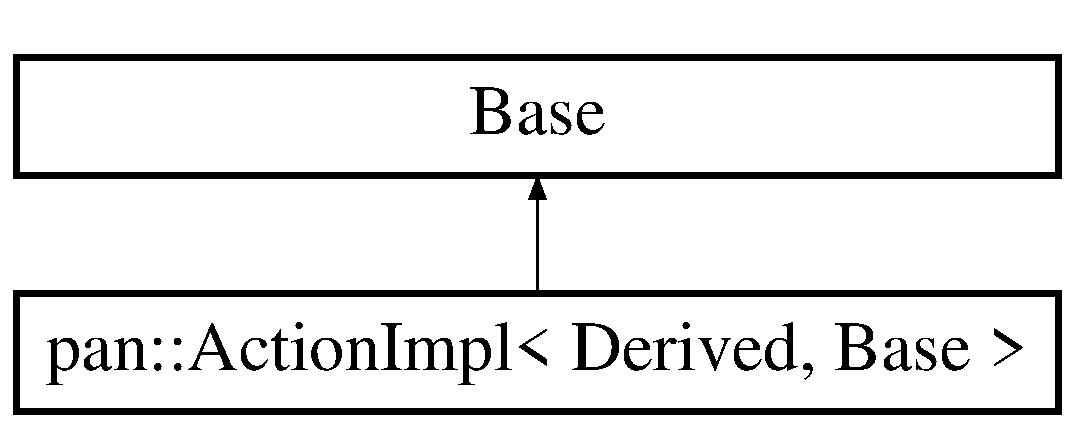
\includegraphics[height=2.000000cm]{classpan_1_1_action_impl}
\end{center}
\end{figure}
\subsection*{Public Member Functions}
\begin{DoxyCompactItemize}
\item 
virtual \hyperlink{classpan_1_1_action_impl_a331fd4215f8a98e88ab05b9e361ce830}{$\sim$\+Action\+Impl} ()
\item 
virtual bool \hyperlink{classpan_1_1_action_impl_acea764a5b41d2fd21717089e21d0c6f4}{validate} (const \hyperlink{classpan_1_1_action_handler}{Action\+Handler} \&h) const
\item 
virtual bool \hyperlink{classpan_1_1_action_impl_a14d72469bea6d60603d49e4815accb54}{execute} (\hyperlink{classpan_1_1_action_handler}{Action\+Handler} \&h) const
\item 
virtual Base $\ast$ \hyperlink{classpan_1_1_action_impl_af94569c5a40d1de5c161282000c1a4c7}{clone} () const
\end{DoxyCompactItemize}


\subsection{Detailed Description}
\subsubsection*{template$<$typename Derived, typename Base$>$\newline
class pan\+::\+Action\+Impl$<$ Derived, Base $>$}

A class containing the implementation of abstract methods of \hyperlink{classpan_1_1_action_base}{Action\+Base}. Subclasses may modify the methods for custom implementation, however it is not needed. 

\begin{DoxyAuthor}{Author}
Hrachya Hakobyan 
\end{DoxyAuthor}


\subsection{Constructor \& Destructor Documentation}
\mbox{\Hypertarget{classpan_1_1_action_impl_a331fd4215f8a98e88ab05b9e361ce830}\label{classpan_1_1_action_impl_a331fd4215f8a98e88ab05b9e361ce830}} 
\index{pan\+::\+Action\+Impl@{pan\+::\+Action\+Impl}!````~Action\+Impl@{$\sim$\+Action\+Impl}}
\index{````~Action\+Impl@{$\sim$\+Action\+Impl}!pan\+::\+Action\+Impl@{pan\+::\+Action\+Impl}}
\subsubsection{\texorpdfstring{$\sim$\+Action\+Impl()}{~ActionImpl()}}
{\footnotesize\ttfamily template$<$typename Derived, typename Base$>$ \\
virtual \hyperlink{classpan_1_1_action_impl}{pan\+::\+Action\+Impl}$<$ Derived, Base $>$\+::$\sim$\hyperlink{classpan_1_1_action_impl}{Action\+Impl} (\begin{DoxyParamCaption}{ }\end{DoxyParamCaption})\hspace{0.3cm}{\ttfamily [inline]}, {\ttfamily [virtual]}}



\subsection{Member Function Documentation}
\mbox{\Hypertarget{classpan_1_1_action_impl_af94569c5a40d1de5c161282000c1a4c7}\label{classpan_1_1_action_impl_af94569c5a40d1de5c161282000c1a4c7}} 
\index{pan\+::\+Action\+Impl@{pan\+::\+Action\+Impl}!clone@{clone}}
\index{clone@{clone}!pan\+::\+Action\+Impl@{pan\+::\+Action\+Impl}}
\subsubsection{\texorpdfstring{clone()}{clone()}}
{\footnotesize\ttfamily template$<$typename Derived, typename Base$>$ \\
virtual Base$\ast$ \hyperlink{classpan_1_1_action_impl}{pan\+::\+Action\+Impl}$<$ Derived, Base $>$\+::clone (\begin{DoxyParamCaption}{ }\end{DoxyParamCaption}) const\hspace{0.3cm}{\ttfamily [inline]}, {\ttfamily [virtual]}}

\mbox{\Hypertarget{classpan_1_1_action_impl_a14d72469bea6d60603d49e4815accb54}\label{classpan_1_1_action_impl_a14d72469bea6d60603d49e4815accb54}} 
\index{pan\+::\+Action\+Impl@{pan\+::\+Action\+Impl}!execute@{execute}}
\index{execute@{execute}!pan\+::\+Action\+Impl@{pan\+::\+Action\+Impl}}
\subsubsection{\texorpdfstring{execute()}{execute()}}
{\footnotesize\ttfamily template$<$typename Derived, typename Base$>$ \\
virtual bool \hyperlink{classpan_1_1_action_impl}{pan\+::\+Action\+Impl}$<$ Derived, Base $>$\+::execute (\begin{DoxyParamCaption}\item[{\hyperlink{classpan_1_1_action_handler}{Action\+Handler} \&}]{h }\end{DoxyParamCaption}) const\hspace{0.3cm}{\ttfamily [inline]}, {\ttfamily [virtual]}}

\mbox{\Hypertarget{classpan_1_1_action_impl_acea764a5b41d2fd21717089e21d0c6f4}\label{classpan_1_1_action_impl_acea764a5b41d2fd21717089e21d0c6f4}} 
\index{pan\+::\+Action\+Impl@{pan\+::\+Action\+Impl}!validate@{validate}}
\index{validate@{validate}!pan\+::\+Action\+Impl@{pan\+::\+Action\+Impl}}
\subsubsection{\texorpdfstring{validate()}{validate()}}
{\footnotesize\ttfamily template$<$typename Derived, typename Base$>$ \\
virtual bool \hyperlink{classpan_1_1_action_impl}{pan\+::\+Action\+Impl}$<$ Derived, Base $>$\+::validate (\begin{DoxyParamCaption}\item[{const \hyperlink{classpan_1_1_action_handler}{Action\+Handler} \&}]{h }\end{DoxyParamCaption}) const\hspace{0.3cm}{\ttfamily [inline]}, {\ttfamily [virtual]}}



The documentation for this class was generated from the following file\+:\begin{DoxyCompactItemize}
\item 
\hyperlink{_action_base_8h}{Action\+Base.\+h}\end{DoxyCompactItemize}

\hypertarget{classpan_1_1_build_research_station}{}\section{pan\+:\+:Build\+Research\+Station Class Reference}
\label{classpan_1_1_build_research_station}\index{pan\+::\+Build\+Research\+Station@{pan\+::\+Build\+Research\+Station}}


Class representing a build research station action.  




{\ttfamily \#include $<$Build\+Research\+Station.\+h$>$}

Inheritance diagram for pan\+:\+:Build\+Research\+Station\+:\begin{figure}[H]
\begin{center}
\leavevmode
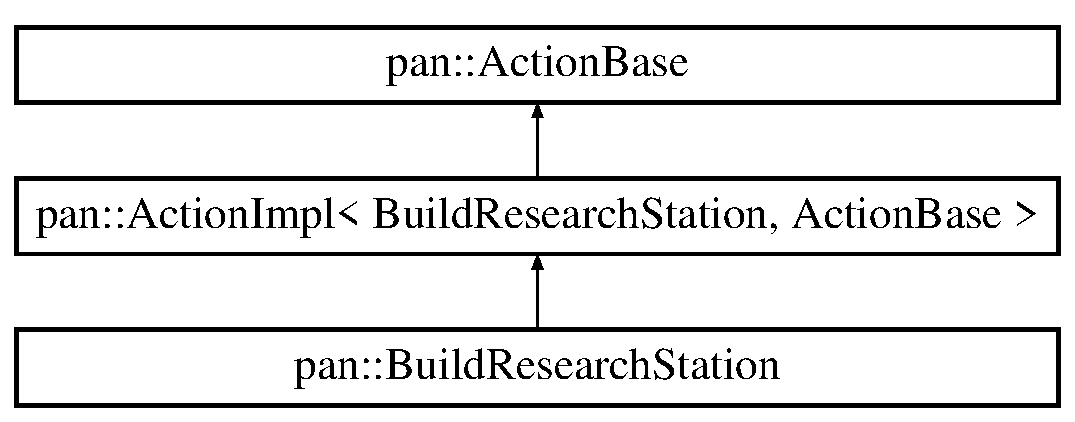
\includegraphics[height=3.000000cm]{classpan_1_1_build_research_station}
\end{center}
\end{figure}
\subsection*{Public Member Functions}
\begin{DoxyCompactItemize}
\item 
\hyperlink{classpan_1_1_build_research_station_a3cd2f5cb3c914c9afa042cd762f46028}{Build\+Research\+Station} (\hyperlink{namespacepan_a0cdabf874fbf1bb3a1f0152d108c2909}{Player\+Index} \hyperlink{classpan_1_1_build_research_station_aa3d64958ccabccec40f25efa85b078a5}{player})
\end{DoxyCompactItemize}
\subsection*{Public Attributes}
\begin{DoxyCompactItemize}
\item 
\hyperlink{namespacepan_a0cdabf874fbf1bb3a1f0152d108c2909}{Player\+Index} \hyperlink{classpan_1_1_build_research_station_aa3d64958ccabccec40f25efa85b078a5}{player}
\end{DoxyCompactItemize}


\subsection{Detailed Description}
Class representing a build research station action. 

\begin{DoxyAuthor}{Author}
Hrachya Hakobyan 
\end{DoxyAuthor}


\subsection{Constructor \& Destructor Documentation}
\mbox{\Hypertarget{classpan_1_1_build_research_station_a3cd2f5cb3c914c9afa042cd762f46028}\label{classpan_1_1_build_research_station_a3cd2f5cb3c914c9afa042cd762f46028}} 
\index{pan\+::\+Build\+Research\+Station@{pan\+::\+Build\+Research\+Station}!Build\+Research\+Station@{Build\+Research\+Station}}
\index{Build\+Research\+Station@{Build\+Research\+Station}!pan\+::\+Build\+Research\+Station@{pan\+::\+Build\+Research\+Station}}
\subsubsection{\texorpdfstring{Build\+Research\+Station()}{BuildResearchStation()}}
{\footnotesize\ttfamily pan\+::\+Build\+Research\+Station\+::\+Build\+Research\+Station (\begin{DoxyParamCaption}\item[{\hyperlink{namespacepan_a0cdabf874fbf1bb3a1f0152d108c2909}{Player\+Index}}]{player }\end{DoxyParamCaption})}



\subsection{Member Data Documentation}
\mbox{\Hypertarget{classpan_1_1_build_research_station_aa3d64958ccabccec40f25efa85b078a5}\label{classpan_1_1_build_research_station_aa3d64958ccabccec40f25efa85b078a5}} 
\index{pan\+::\+Build\+Research\+Station@{pan\+::\+Build\+Research\+Station}!player@{player}}
\index{player@{player}!pan\+::\+Build\+Research\+Station@{pan\+::\+Build\+Research\+Station}}
\subsubsection{\texorpdfstring{player}{player}}
{\footnotesize\ttfamily \hyperlink{namespacepan_a0cdabf874fbf1bb3a1f0152d108c2909}{Player\+Index} pan\+::\+Build\+Research\+Station\+::player}



The documentation for this class was generated from the following files\+:\begin{DoxyCompactItemize}
\item 
\hyperlink{_build_research_station_8h}{Build\+Research\+Station.\+h}\item 
\hyperlink{_build_research_station_8cpp}{Build\+Research\+Station.\+cpp}\end{DoxyCompactItemize}

\hypertarget{classpan_1_1_card_base}{}\section{pan\+:\+:Card\+Base Class Reference}
\label{classpan_1_1_card_base}\index{pan\+::\+Card\+Base@{pan\+::\+Card\+Base}}


Abstract class to represent Card entity in the game. Cards contain an enum to differentiate their type.  




{\ttfamily \#include $<$Card.\+h$>$}

Inheritance diagram for pan\+:\+:Card\+Base\+:\begin{figure}[H]
\begin{center}
\leavevmode
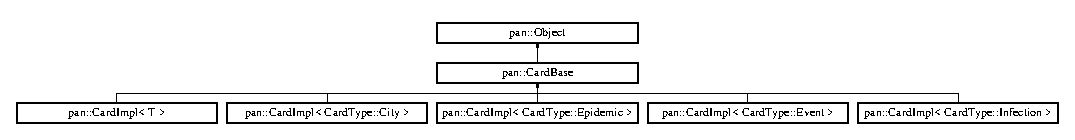
\includegraphics[height=1.435897cm]{classpan_1_1_card_base}
\end{center}
\end{figure}
\subsection*{Public Member Functions}
\begin{DoxyCompactItemize}
\item 
virtual \hyperlink{classpan_1_1_card_base_a85b2e83d4d62dad2f43a91277cbdf974}{$\sim$\+Card\+Base} ()=default
\item 
bool \hyperlink{classpan_1_1_card_base_a21cc5a1c879b848d21d2a579cfcadd19}{operator==} (const \hyperlink{classpan_1_1_card_base}{Card\+Base} \&) const
\item 
bool \hyperlink{classpan_1_1_card_base_a2f71f627f9f4b04fbe0982667a513728}{operator!=} (const \hyperlink{classpan_1_1_card_base}{Card\+Base} \&) const
\item 
virtual std\+::string \hyperlink{classpan_1_1_card_base_ad004c502404a958eaf4ecae7e73cc8cf}{description} () const
\item 
\hyperlink{classpan_1_1_card_base_afdca48b95924340316fd8a0a0a784330}{Card\+Base} (\hyperlink{namespacepan_a1f7350bfd0421afeabe9fa95c16fa811}{Card\+Type} \hyperlink{classpan_1_1_card_base_a47c25b9584c70305e862fcab7d0212ee}{type})
\item 
virtual bool \hyperlink{classpan_1_1_card_base_aaf967cee010ef974699da8502834e0e6}{equals} (const \hyperlink{classpan_1_1_card_base}{Card\+Base} \&) const
\end{DoxyCompactItemize}
\subsection*{Public Attributes}
\begin{DoxyCompactItemize}
\item 
const \hyperlink{namespacepan_a1f7350bfd0421afeabe9fa95c16fa811}{Card\+Type} \hyperlink{classpan_1_1_card_base_a47c25b9584c70305e862fcab7d0212ee}{type}
\end{DoxyCompactItemize}
\subsection*{Friends}
\begin{DoxyCompactItemize}
\item 
class \hyperlink{classpan_1_1_card_base_ac98d07dd8f7b70e16ccb9a01abf56b9c}{boost\+::serialization\+::access}
\end{DoxyCompactItemize}


\subsection{Detailed Description}
Abstract class to represent Card entity in the game. Cards contain an enum to differentiate their type. 

\begin{DoxyAuthor}{Author}
Hrachya Hakobyan 
\end{DoxyAuthor}


\subsection{Constructor \& Destructor Documentation}
\mbox{\Hypertarget{classpan_1_1_card_base_a85b2e83d4d62dad2f43a91277cbdf974}\label{classpan_1_1_card_base_a85b2e83d4d62dad2f43a91277cbdf974}} 
\index{pan\+::\+Card\+Base@{pan\+::\+Card\+Base}!````~Card\+Base@{$\sim$\+Card\+Base}}
\index{````~Card\+Base@{$\sim$\+Card\+Base}!pan\+::\+Card\+Base@{pan\+::\+Card\+Base}}
\subsubsection{\texorpdfstring{$\sim$\+Card\+Base()}{~CardBase()}}
{\footnotesize\ttfamily virtual pan\+::\+Card\+Base\+::$\sim$\+Card\+Base (\begin{DoxyParamCaption}{ }\end{DoxyParamCaption})\hspace{0.3cm}{\ttfamily [virtual]}, {\ttfamily [default]}}

\mbox{\Hypertarget{classpan_1_1_card_base_afdca48b95924340316fd8a0a0a784330}\label{classpan_1_1_card_base_afdca48b95924340316fd8a0a0a784330}} 
\index{pan\+::\+Card\+Base@{pan\+::\+Card\+Base}!Card\+Base@{Card\+Base}}
\index{Card\+Base@{Card\+Base}!pan\+::\+Card\+Base@{pan\+::\+Card\+Base}}
\subsubsection{\texorpdfstring{Card\+Base()}{CardBase()}}
{\footnotesize\ttfamily pan\+::\+Card\+Base\+::\+Card\+Base (\begin{DoxyParamCaption}\item[{\hyperlink{namespacepan_a1f7350bfd0421afeabe9fa95c16fa811}{Card\+Type}}]{type }\end{DoxyParamCaption})}



\subsection{Member Function Documentation}
\mbox{\Hypertarget{classpan_1_1_card_base_ad004c502404a958eaf4ecae7e73cc8cf}\label{classpan_1_1_card_base_ad004c502404a958eaf4ecae7e73cc8cf}} 
\index{pan\+::\+Card\+Base@{pan\+::\+Card\+Base}!description@{description}}
\index{description@{description}!pan\+::\+Card\+Base@{pan\+::\+Card\+Base}}
\subsubsection{\texorpdfstring{description()}{description()}}
{\footnotesize\ttfamily std\+::string pan\+::\+Card\+Base\+::description (\begin{DoxyParamCaption}{ }\end{DoxyParamCaption}) const\hspace{0.3cm}{\ttfamily [virtual]}}



Implements \hyperlink{classpan_1_1_object_a2bb6d3117bb32f5774657c83f118ed8b}{pan\+::\+Object}.



Reimplemented in \hyperlink{classpan_1_1_card_impl_3_01_card_type_1_1_event_01_4_aa5c7d2729e0bfb141a0d8487a590a580}{pan\+::\+Card\+Impl$<$ Card\+Type\+::\+Event $>$}, \hyperlink{classpan_1_1_card_impl_3_01_card_type_1_1_city_01_4_a326c3eaac225bd758f19abb152deffe4}{pan\+::\+Card\+Impl$<$ Card\+Type\+::\+City $>$}, and \hyperlink{classpan_1_1_card_impl_3_01_card_type_1_1_infection_01_4_a5e31904120b655ce59633433a4d4c17c}{pan\+::\+Card\+Impl$<$ Card\+Type\+::\+Infection $>$}.

\mbox{\Hypertarget{classpan_1_1_card_base_aaf967cee010ef974699da8502834e0e6}\label{classpan_1_1_card_base_aaf967cee010ef974699da8502834e0e6}} 
\index{pan\+::\+Card\+Base@{pan\+::\+Card\+Base}!equals@{equals}}
\index{equals@{equals}!pan\+::\+Card\+Base@{pan\+::\+Card\+Base}}
\subsubsection{\texorpdfstring{equals()}{equals()}}
{\footnotesize\ttfamily virtual bool pan\+::\+Card\+Base\+::equals (\begin{DoxyParamCaption}\item[{const \hyperlink{classpan_1_1_card_base}{Card\+Base} \&}]{ }\end{DoxyParamCaption}) const\hspace{0.3cm}{\ttfamily [inline]}, {\ttfamily [virtual]}}

\mbox{\Hypertarget{classpan_1_1_card_base_a2f71f627f9f4b04fbe0982667a513728}\label{classpan_1_1_card_base_a2f71f627f9f4b04fbe0982667a513728}} 
\index{pan\+::\+Card\+Base@{pan\+::\+Card\+Base}!operator"!=@{operator"!=}}
\index{operator"!=@{operator"!=}!pan\+::\+Card\+Base@{pan\+::\+Card\+Base}}
\subsubsection{\texorpdfstring{operator"!=()}{operator!=()}}
{\footnotesize\ttfamily bool pan\+::\+Card\+Base\+::operator!= (\begin{DoxyParamCaption}\item[{const \hyperlink{classpan_1_1_card_base}{Card\+Base} \&}]{o }\end{DoxyParamCaption}) const\hspace{0.3cm}{\ttfamily [inline]}}

\mbox{\Hypertarget{classpan_1_1_card_base_a21cc5a1c879b848d21d2a579cfcadd19}\label{classpan_1_1_card_base_a21cc5a1c879b848d21d2a579cfcadd19}} 
\index{pan\+::\+Card\+Base@{pan\+::\+Card\+Base}!operator==@{operator==}}
\index{operator==@{operator==}!pan\+::\+Card\+Base@{pan\+::\+Card\+Base}}
\subsubsection{\texorpdfstring{operator==()}{operator==()}}
{\footnotesize\ttfamily bool pan\+::\+Card\+Base\+::operator== (\begin{DoxyParamCaption}\item[{const \hyperlink{classpan_1_1_card_base}{Card\+Base} \&}]{o }\end{DoxyParamCaption}) const}



\subsection{Friends And Related Function Documentation}
\mbox{\Hypertarget{classpan_1_1_card_base_ac98d07dd8f7b70e16ccb9a01abf56b9c}\label{classpan_1_1_card_base_ac98d07dd8f7b70e16ccb9a01abf56b9c}} 
\index{pan\+::\+Card\+Base@{pan\+::\+Card\+Base}!boost\+::serialization\+::access@{boost\+::serialization\+::access}}
\index{boost\+::serialization\+::access@{boost\+::serialization\+::access}!pan\+::\+Card\+Base@{pan\+::\+Card\+Base}}
\subsubsection{\texorpdfstring{boost\+::serialization\+::access}{boost::serialization::access}}
{\footnotesize\ttfamily friend class boost\+::serialization\+::access\hspace{0.3cm}{\ttfamily [friend]}}



\subsection{Member Data Documentation}
\mbox{\Hypertarget{classpan_1_1_card_base_a47c25b9584c70305e862fcab7d0212ee}\label{classpan_1_1_card_base_a47c25b9584c70305e862fcab7d0212ee}} 
\index{pan\+::\+Card\+Base@{pan\+::\+Card\+Base}!type@{type}}
\index{type@{type}!pan\+::\+Card\+Base@{pan\+::\+Card\+Base}}
\subsubsection{\texorpdfstring{type}{type}}
{\footnotesize\ttfamily const \hyperlink{namespacepan_a1f7350bfd0421afeabe9fa95c16fa811}{Card\+Type} pan\+::\+Card\+Base\+::type}



The documentation for this class was generated from the following files\+:\begin{DoxyCompactItemize}
\item 
\hyperlink{_card_8h}{Card.\+h}\item 
\hyperlink{_card_8cpp}{Card.\+cpp}\end{DoxyCompactItemize}

\hypertarget{classpan_1_1_card_impl}{}\section{pan\+:\+:Card\+Impl$<$ T $>$ Class Template Reference}
\label{classpan_1_1_card_impl}\index{pan\+::\+Card\+Impl$<$ T $>$@{pan\+::\+Card\+Impl$<$ T $>$}}


{\ttfamily \#include $<$Card.\+h$>$}

Inheritance diagram for pan\+:\+:Card\+Impl$<$ T $>$\+:\begin{figure}[H]
\begin{center}
\leavevmode
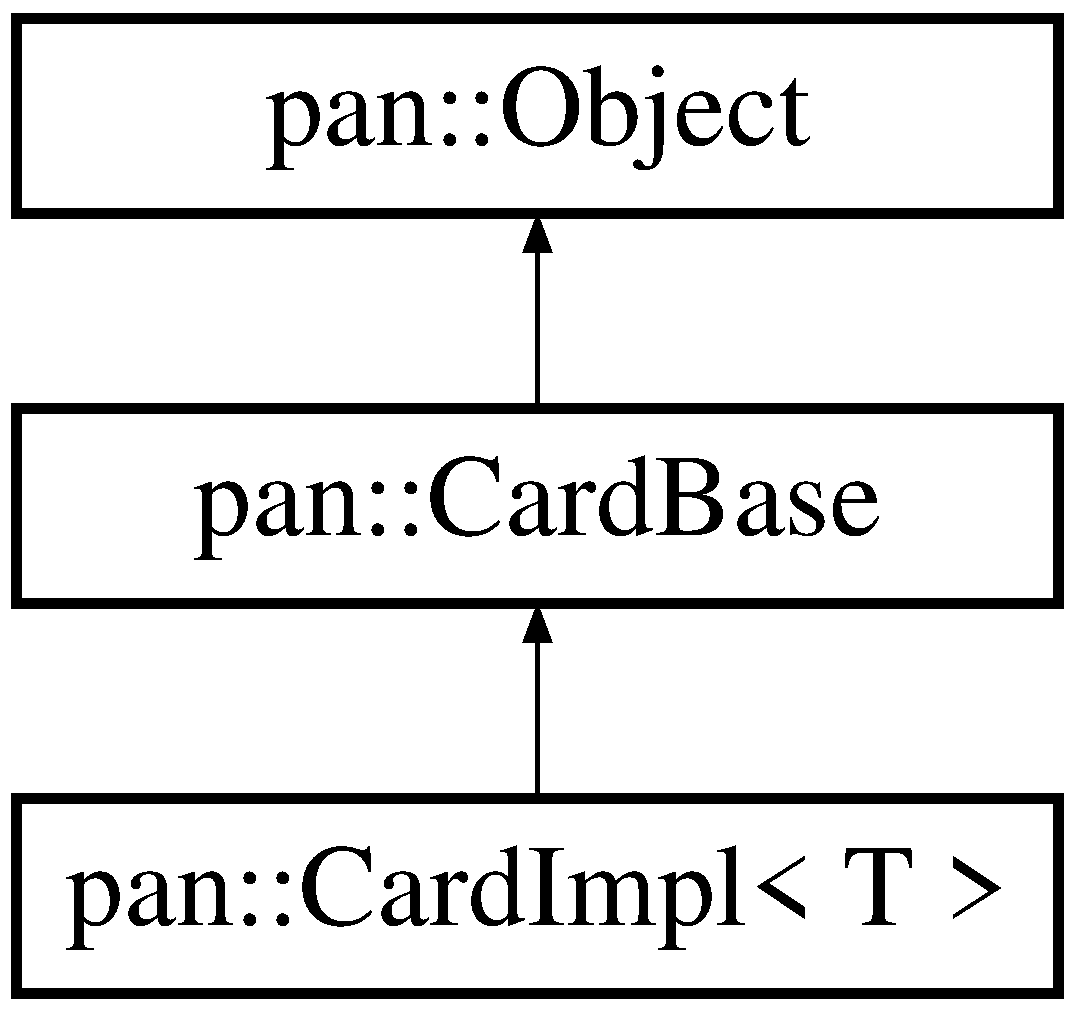
\includegraphics[height=3.000000cm]{classpan_1_1_card_impl}
\end{center}
\end{figure}
\subsection*{Additional Inherited Members}


The documentation for this class was generated from the following file\+:\begin{DoxyCompactItemize}
\item 
\hyperlink{_card_8h}{Card.\+h}\end{DoxyCompactItemize}

\hypertarget{classpan_1_1_card_impl_3_01_card_type_1_1_city_01_4}{}\section{pan\+:\+:Card\+Impl$<$ Card\+Type\+:\+:City $>$ Class Template Reference}
\label{classpan_1_1_card_impl_3_01_card_type_1_1_city_01_4}\index{pan\+::\+Card\+Impl$<$ Card\+Type\+::\+City $>$@{pan\+::\+Card\+Impl$<$ Card\+Type\+::\+City $>$}}


Represents the \hyperlink{classpan_1_1_city}{City} card entity.  




{\ttfamily \#include $<$City\+Card.\+h$>$}

Inheritance diagram for pan\+:\+:Card\+Impl$<$ Card\+Type\+:\+:City $>$\+:\begin{figure}[H]
\begin{center}
\leavevmode
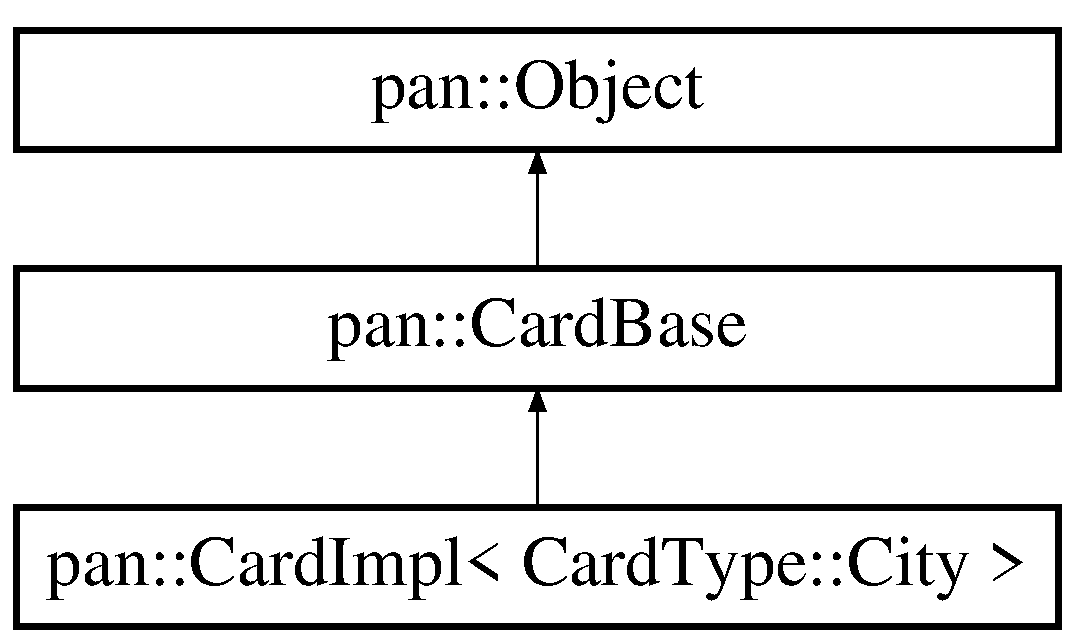
\includegraphics[height=3.000000cm]{classpan_1_1_card_impl_3_01_card_type_1_1_city_01_4}
\end{center}
\end{figure}
\subsection*{Public Member Functions}
\begin{DoxyCompactItemize}
\item 
\hyperlink{classpan_1_1_card_impl_3_01_card_type_1_1_city_01_4_a9377dcb4087c82ccb0f021e0a675e9e3}{Card\+Impl} (\hyperlink{namespacepan_afaed28aa6603153dcc062a028602d697}{City\+Index} index)
\item 
\hyperlink{classpan_1_1_card_impl_3_01_card_type_1_1_city_01_4_afae904aca39e8e484641db88448e308c}{$\sim$\+Card\+Impl} ()=default
\item 
std\+::string \hyperlink{classpan_1_1_card_impl_3_01_card_type_1_1_city_01_4_a326c3eaac225bd758f19abb152deffe4}{description} () const
\item 
bool \hyperlink{classpan_1_1_card_impl_3_01_card_type_1_1_city_01_4_a7cabd76cb3e639248244e84e09bfe341}{operator==} (const \hyperlink{classpan_1_1_card_impl}{Card\+Impl} \&) const
\item 
bool \hyperlink{classpan_1_1_card_impl_3_01_card_type_1_1_city_01_4_a74d7d8382dd0d197800b24d9c22547d9}{operator!=} (const \hyperlink{classpan_1_1_card_impl}{Card\+Impl} \&) const
\end{DoxyCompactItemize}
\subsection*{Public Attributes}
\begin{DoxyCompactItemize}
\item 
const \hyperlink{namespacepan_afaed28aa6603153dcc062a028602d697}{City\+Index} \hyperlink{classpan_1_1_card_impl_3_01_card_type_1_1_city_01_4_a793e709dc8efad7f513a1b92079ac09b}{city\+Index}
\end{DoxyCompactItemize}
\subsection*{Friends}
\begin{DoxyCompactItemize}
\item 
class \hyperlink{classpan_1_1_card_impl_3_01_card_type_1_1_city_01_4_ac98d07dd8f7b70e16ccb9a01abf56b9c}{boost\+::serialization\+::access}
\end{DoxyCompactItemize}


\subsection{Detailed Description}
\subsubsection*{template$<$$>$\newline
class pan\+::\+Card\+Impl$<$ Card\+Type\+::\+City $>$}

Represents the \hyperlink{classpan_1_1_city}{City} card entity. 

\begin{DoxyAuthor}{Author}
Hrachya Hakobyan 
\end{DoxyAuthor}


\subsection{Constructor \& Destructor Documentation}
\mbox{\Hypertarget{classpan_1_1_card_impl_3_01_card_type_1_1_city_01_4_a9377dcb4087c82ccb0f021e0a675e9e3}\label{classpan_1_1_card_impl_3_01_card_type_1_1_city_01_4_a9377dcb4087c82ccb0f021e0a675e9e3}} 
\index{pan\+::\+Card\+Impl$<$ Card\+Type\+::\+City $>$@{pan\+::\+Card\+Impl$<$ Card\+Type\+::\+City $>$}!Card\+Impl@{Card\+Impl}}
\index{Card\+Impl@{Card\+Impl}!pan\+::\+Card\+Impl$<$ Card\+Type\+::\+City $>$@{pan\+::\+Card\+Impl$<$ Card\+Type\+::\+City $>$}}
\subsubsection{\texorpdfstring{Card\+Impl()}{CardImpl()}}
{\footnotesize\ttfamily \hyperlink{classpan_1_1_card_impl}{pan\+::\+Card\+Impl}$<$ \hyperlink{namespacepan_a1f7350bfd0421afeabe9fa95c16fa811a57d056ed0984166336b7879c2af3657f}{Card\+Type\+::\+City} $>$\+::\hyperlink{classpan_1_1_card_impl}{Card\+Impl} (\begin{DoxyParamCaption}\item[{\hyperlink{namespacepan_afaed28aa6603153dcc062a028602d697}{City\+Index}}]{index }\end{DoxyParamCaption})}

\mbox{\Hypertarget{classpan_1_1_card_impl_3_01_card_type_1_1_city_01_4_afae904aca39e8e484641db88448e308c}\label{classpan_1_1_card_impl_3_01_card_type_1_1_city_01_4_afae904aca39e8e484641db88448e308c}} 
\index{pan\+::\+Card\+Impl$<$ Card\+Type\+::\+City $>$@{pan\+::\+Card\+Impl$<$ Card\+Type\+::\+City $>$}!````~Card\+Impl@{$\sim$\+Card\+Impl}}
\index{````~Card\+Impl@{$\sim$\+Card\+Impl}!pan\+::\+Card\+Impl$<$ Card\+Type\+::\+City $>$@{pan\+::\+Card\+Impl$<$ Card\+Type\+::\+City $>$}}
\subsubsection{\texorpdfstring{$\sim$\+Card\+Impl()}{~CardImpl()}}
{\footnotesize\ttfamily \hyperlink{classpan_1_1_card_impl}{pan\+::\+Card\+Impl}$<$ \hyperlink{namespacepan_a1f7350bfd0421afeabe9fa95c16fa811a57d056ed0984166336b7879c2af3657f}{Card\+Type\+::\+City} $>$\+::$\sim$\hyperlink{classpan_1_1_card_impl}{Card\+Impl} (\begin{DoxyParamCaption}{ }\end{DoxyParamCaption})\hspace{0.3cm}{\ttfamily [default]}}



\subsection{Member Function Documentation}
\mbox{\Hypertarget{classpan_1_1_card_impl_3_01_card_type_1_1_city_01_4_a326c3eaac225bd758f19abb152deffe4}\label{classpan_1_1_card_impl_3_01_card_type_1_1_city_01_4_a326c3eaac225bd758f19abb152deffe4}} 
\index{pan\+::\+Card\+Impl$<$ Card\+Type\+::\+City $>$@{pan\+::\+Card\+Impl$<$ Card\+Type\+::\+City $>$}!description@{description}}
\index{description@{description}!pan\+::\+Card\+Impl$<$ Card\+Type\+::\+City $>$@{pan\+::\+Card\+Impl$<$ Card\+Type\+::\+City $>$}}
\subsubsection{\texorpdfstring{description()}{description()}}
{\footnotesize\ttfamily std\+::string \hyperlink{classpan_1_1_card_impl}{pan\+::\+Card\+Impl}$<$ \hyperlink{namespacepan_a1f7350bfd0421afeabe9fa95c16fa811a57d056ed0984166336b7879c2af3657f}{Card\+Type\+::\+City} $>$\+::description (\begin{DoxyParamCaption}{ }\end{DoxyParamCaption}) const\hspace{0.3cm}{\ttfamily [inline]}, {\ttfamily [virtual]}}



Reimplemented from \hyperlink{classpan_1_1_card_base_ad004c502404a958eaf4ecae7e73cc8cf}{pan\+::\+Card\+Base}.

\mbox{\Hypertarget{classpan_1_1_card_impl_3_01_card_type_1_1_city_01_4_a74d7d8382dd0d197800b24d9c22547d9}\label{classpan_1_1_card_impl_3_01_card_type_1_1_city_01_4_a74d7d8382dd0d197800b24d9c22547d9}} 
\index{pan\+::\+Card\+Impl$<$ Card\+Type\+::\+City $>$@{pan\+::\+Card\+Impl$<$ Card\+Type\+::\+City $>$}!operator"!=@{operator"!=}}
\index{operator"!=@{operator"!=}!pan\+::\+Card\+Impl$<$ Card\+Type\+::\+City $>$@{pan\+::\+Card\+Impl$<$ Card\+Type\+::\+City $>$}}
\subsubsection{\texorpdfstring{operator"!=()}{operator!=()}}
{\footnotesize\ttfamily bool \hyperlink{classpan_1_1_card_impl}{pan\+::\+Card\+Impl}$<$ \hyperlink{namespacepan_a1f7350bfd0421afeabe9fa95c16fa811a57d056ed0984166336b7879c2af3657f}{Card\+Type\+::\+City} $>$\+::operator!= (\begin{DoxyParamCaption}\item[{const \hyperlink{classpan_1_1_card_impl}{Card\+Impl}$<$ \hyperlink{namespacepan_a1f7350bfd0421afeabe9fa95c16fa811a57d056ed0984166336b7879c2af3657f}{Card\+Type\+::\+City} $>$ \&}]{o }\end{DoxyParamCaption}) const\hspace{0.3cm}{\ttfamily [inline]}}

\mbox{\Hypertarget{classpan_1_1_card_impl_3_01_card_type_1_1_city_01_4_a7cabd76cb3e639248244e84e09bfe341}\label{classpan_1_1_card_impl_3_01_card_type_1_1_city_01_4_a7cabd76cb3e639248244e84e09bfe341}} 
\index{pan\+::\+Card\+Impl$<$ Card\+Type\+::\+City $>$@{pan\+::\+Card\+Impl$<$ Card\+Type\+::\+City $>$}!operator==@{operator==}}
\index{operator==@{operator==}!pan\+::\+Card\+Impl$<$ Card\+Type\+::\+City $>$@{pan\+::\+Card\+Impl$<$ Card\+Type\+::\+City $>$}}
\subsubsection{\texorpdfstring{operator==()}{operator==()}}
{\footnotesize\ttfamily bool \hyperlink{classpan_1_1_card_impl}{pan\+::\+Card\+Impl}$<$ \hyperlink{namespacepan_a1f7350bfd0421afeabe9fa95c16fa811a57d056ed0984166336b7879c2af3657f}{Card\+Type\+::\+City} $>$\+::operator== (\begin{DoxyParamCaption}\item[{const \hyperlink{classpan_1_1_card_impl}{Card\+Impl}$<$ \hyperlink{namespacepan_a1f7350bfd0421afeabe9fa95c16fa811a57d056ed0984166336b7879c2af3657f}{Card\+Type\+::\+City} $>$ \&}]{o }\end{DoxyParamCaption}) const\hspace{0.3cm}{\ttfamily [inline]}}



\subsection{Friends And Related Function Documentation}
\mbox{\Hypertarget{classpan_1_1_card_impl_3_01_card_type_1_1_city_01_4_ac98d07dd8f7b70e16ccb9a01abf56b9c}\label{classpan_1_1_card_impl_3_01_card_type_1_1_city_01_4_ac98d07dd8f7b70e16ccb9a01abf56b9c}} 
\index{pan\+::\+Card\+Impl$<$ Card\+Type\+::\+City $>$@{pan\+::\+Card\+Impl$<$ Card\+Type\+::\+City $>$}!boost\+::serialization\+::access@{boost\+::serialization\+::access}}
\index{boost\+::serialization\+::access@{boost\+::serialization\+::access}!pan\+::\+Card\+Impl$<$ Card\+Type\+::\+City $>$@{pan\+::\+Card\+Impl$<$ Card\+Type\+::\+City $>$}}
\subsubsection{\texorpdfstring{boost\+::serialization\+::access}{boost::serialization::access}}
{\footnotesize\ttfamily friend class boost\+::serialization\+::access\hspace{0.3cm}{\ttfamily [friend]}}



\subsection{Member Data Documentation}
\mbox{\Hypertarget{classpan_1_1_card_impl_3_01_card_type_1_1_city_01_4_a793e709dc8efad7f513a1b92079ac09b}\label{classpan_1_1_card_impl_3_01_card_type_1_1_city_01_4_a793e709dc8efad7f513a1b92079ac09b}} 
\index{pan\+::\+Card\+Impl$<$ Card\+Type\+::\+City $>$@{pan\+::\+Card\+Impl$<$ Card\+Type\+::\+City $>$}!city\+Index@{city\+Index}}
\index{city\+Index@{city\+Index}!pan\+::\+Card\+Impl$<$ Card\+Type\+::\+City $>$@{pan\+::\+Card\+Impl$<$ Card\+Type\+::\+City $>$}}
\subsubsection{\texorpdfstring{city\+Index}{cityIndex}}
{\footnotesize\ttfamily const \hyperlink{namespacepan_afaed28aa6603153dcc062a028602d697}{City\+Index} \hyperlink{classpan_1_1_card_impl}{pan\+::\+Card\+Impl}$<$ \hyperlink{namespacepan_a1f7350bfd0421afeabe9fa95c16fa811a57d056ed0984166336b7879c2af3657f}{Card\+Type\+::\+City} $>$\+::city\+Index}



The documentation for this class was generated from the following files\+:\begin{DoxyCompactItemize}
\item 
\hyperlink{_city_card_8h}{City\+Card.\+h}\item 
\hyperlink{_city_card_8cpp}{City\+Card.\+cpp}\end{DoxyCompactItemize}

\hypertarget{classpan_1_1_card_impl_3_01_card_type_1_1_epidemic_01_4}{}\section{pan\+:\+:Card\+Impl$<$ Card\+Type\+:\+:Epidemic $>$ Class Template Reference}
\label{classpan_1_1_card_impl_3_01_card_type_1_1_epidemic_01_4}\index{pan\+::\+Card\+Impl$<$ Card\+Type\+::\+Epidemic $>$@{pan\+::\+Card\+Impl$<$ Card\+Type\+::\+Epidemic $>$}}


Represents the \hyperlink{classpan_1_1_epidemic}{Epidemic} card entity.  




{\ttfamily \#include $<$Epidemic\+Card.\+h$>$}

Inheritance diagram for pan\+:\+:Card\+Impl$<$ Card\+Type\+:\+:Epidemic $>$\+:\begin{figure}[H]
\begin{center}
\leavevmode
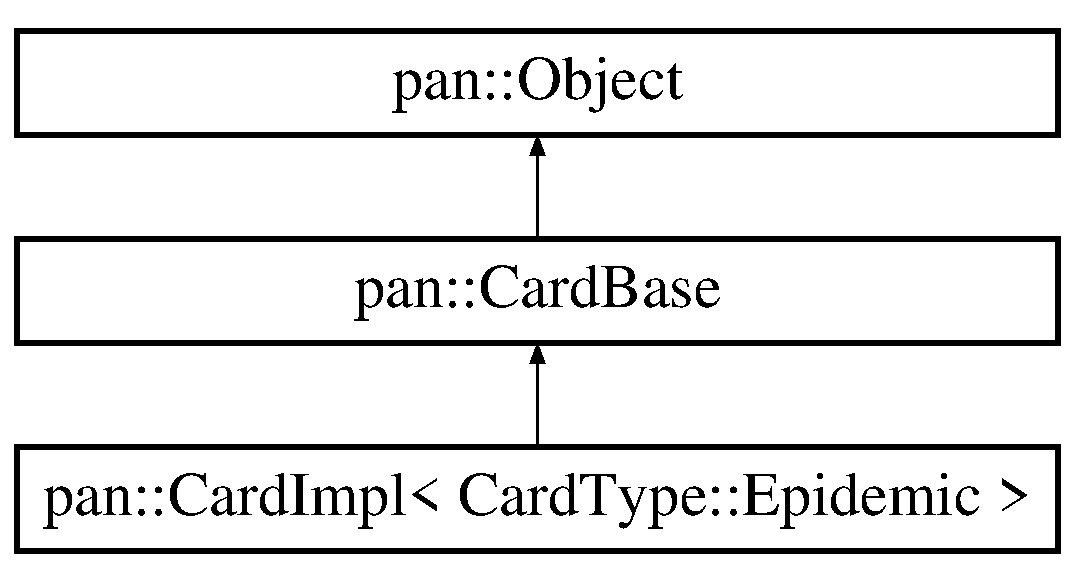
\includegraphics[height=3.000000cm]{classpan_1_1_card_impl_3_01_card_type_1_1_epidemic_01_4}
\end{center}
\end{figure}
\subsection*{Public Member Functions}
\begin{DoxyCompactItemize}
\item 
\hyperlink{classpan_1_1_card_impl_3_01_card_type_1_1_epidemic_01_4_a19cabff4b96d1931e1ef0332c28eee92}{Card\+Impl} ()
\item 
\hyperlink{classpan_1_1_card_impl_3_01_card_type_1_1_epidemic_01_4_a1af8f6b83d5ff973c3480854e0ee290d}{$\sim$\+Card\+Impl} ()=default
\item 
bool \hyperlink{classpan_1_1_card_impl_3_01_card_type_1_1_epidemic_01_4_a90424e537b2e228c367f1b107cc39e4c}{operator==} (const \hyperlink{classpan_1_1_card_impl}{Card\+Impl} \&) const
\item 
bool \hyperlink{classpan_1_1_card_impl_3_01_card_type_1_1_epidemic_01_4_a812d96882f6e80e71260ca7fef95f421}{operator!=} (const \hyperlink{classpan_1_1_card_impl}{Card\+Impl} \&) const
\end{DoxyCompactItemize}
\subsection*{Friends}
\begin{DoxyCompactItemize}
\item 
class \hyperlink{classpan_1_1_card_impl_3_01_card_type_1_1_epidemic_01_4_ac98d07dd8f7b70e16ccb9a01abf56b9c}{boost\+::serialization\+::access}
\end{DoxyCompactItemize}
\subsection*{Additional Inherited Members}


\subsection{Detailed Description}
\subsubsection*{template$<$$>$\newline
class pan\+::\+Card\+Impl$<$ Card\+Type\+::\+Epidemic $>$}

Represents the \hyperlink{classpan_1_1_epidemic}{Epidemic} card entity. 

\begin{DoxyAuthor}{Author}
Hrachya Hakobyan 
\end{DoxyAuthor}


\subsection{Constructor \& Destructor Documentation}
\mbox{\Hypertarget{classpan_1_1_card_impl_3_01_card_type_1_1_epidemic_01_4_a19cabff4b96d1931e1ef0332c28eee92}\label{classpan_1_1_card_impl_3_01_card_type_1_1_epidemic_01_4_a19cabff4b96d1931e1ef0332c28eee92}} 
\index{pan\+::\+Card\+Impl$<$ Card\+Type\+::\+Epidemic $>$@{pan\+::\+Card\+Impl$<$ Card\+Type\+::\+Epidemic $>$}!Card\+Impl@{Card\+Impl}}
\index{Card\+Impl@{Card\+Impl}!pan\+::\+Card\+Impl$<$ Card\+Type\+::\+Epidemic $>$@{pan\+::\+Card\+Impl$<$ Card\+Type\+::\+Epidemic $>$}}
\subsubsection{\texorpdfstring{Card\+Impl()}{CardImpl()}}
{\footnotesize\ttfamily \hyperlink{classpan_1_1_card_impl}{pan\+::\+Card\+Impl}$<$ \hyperlink{namespacepan_a1f7350bfd0421afeabe9fa95c16fa811a62eff626cf0804badc417196cfd09a12}{Card\+Type\+::\+Epidemic} $>$\+::\hyperlink{classpan_1_1_card_impl}{Card\+Impl} (\begin{DoxyParamCaption}{ }\end{DoxyParamCaption})}

\mbox{\Hypertarget{classpan_1_1_card_impl_3_01_card_type_1_1_epidemic_01_4_a1af8f6b83d5ff973c3480854e0ee290d}\label{classpan_1_1_card_impl_3_01_card_type_1_1_epidemic_01_4_a1af8f6b83d5ff973c3480854e0ee290d}} 
\index{pan\+::\+Card\+Impl$<$ Card\+Type\+::\+Epidemic $>$@{pan\+::\+Card\+Impl$<$ Card\+Type\+::\+Epidemic $>$}!````~Card\+Impl@{$\sim$\+Card\+Impl}}
\index{````~Card\+Impl@{$\sim$\+Card\+Impl}!pan\+::\+Card\+Impl$<$ Card\+Type\+::\+Epidemic $>$@{pan\+::\+Card\+Impl$<$ Card\+Type\+::\+Epidemic $>$}}
\subsubsection{\texorpdfstring{$\sim$\+Card\+Impl()}{~CardImpl()}}
{\footnotesize\ttfamily \hyperlink{classpan_1_1_card_impl}{pan\+::\+Card\+Impl}$<$ \hyperlink{namespacepan_a1f7350bfd0421afeabe9fa95c16fa811a62eff626cf0804badc417196cfd09a12}{Card\+Type\+::\+Epidemic} $>$\+::$\sim$\hyperlink{classpan_1_1_card_impl}{Card\+Impl} (\begin{DoxyParamCaption}{ }\end{DoxyParamCaption})\hspace{0.3cm}{\ttfamily [default]}}



\subsection{Member Function Documentation}
\mbox{\Hypertarget{classpan_1_1_card_impl_3_01_card_type_1_1_epidemic_01_4_a812d96882f6e80e71260ca7fef95f421}\label{classpan_1_1_card_impl_3_01_card_type_1_1_epidemic_01_4_a812d96882f6e80e71260ca7fef95f421}} 
\index{pan\+::\+Card\+Impl$<$ Card\+Type\+::\+Epidemic $>$@{pan\+::\+Card\+Impl$<$ Card\+Type\+::\+Epidemic $>$}!operator"!=@{operator"!=}}
\index{operator"!=@{operator"!=}!pan\+::\+Card\+Impl$<$ Card\+Type\+::\+Epidemic $>$@{pan\+::\+Card\+Impl$<$ Card\+Type\+::\+Epidemic $>$}}
\subsubsection{\texorpdfstring{operator"!=()}{operator!=()}}
{\footnotesize\ttfamily bool \hyperlink{classpan_1_1_card_impl}{pan\+::\+Card\+Impl}$<$ \hyperlink{namespacepan_a1f7350bfd0421afeabe9fa95c16fa811a62eff626cf0804badc417196cfd09a12}{Card\+Type\+::\+Epidemic} $>$\+::operator!= (\begin{DoxyParamCaption}\item[{const \hyperlink{classpan_1_1_card_impl}{Card\+Impl}$<$ \hyperlink{namespacepan_a1f7350bfd0421afeabe9fa95c16fa811a62eff626cf0804badc417196cfd09a12}{Card\+Type\+::\+Epidemic} $>$ \&}]{o }\end{DoxyParamCaption}) const\hspace{0.3cm}{\ttfamily [inline]}}

\mbox{\Hypertarget{classpan_1_1_card_impl_3_01_card_type_1_1_epidemic_01_4_a90424e537b2e228c367f1b107cc39e4c}\label{classpan_1_1_card_impl_3_01_card_type_1_1_epidemic_01_4_a90424e537b2e228c367f1b107cc39e4c}} 
\index{pan\+::\+Card\+Impl$<$ Card\+Type\+::\+Epidemic $>$@{pan\+::\+Card\+Impl$<$ Card\+Type\+::\+Epidemic $>$}!operator==@{operator==}}
\index{operator==@{operator==}!pan\+::\+Card\+Impl$<$ Card\+Type\+::\+Epidemic $>$@{pan\+::\+Card\+Impl$<$ Card\+Type\+::\+Epidemic $>$}}
\subsubsection{\texorpdfstring{operator==()}{operator==()}}
{\footnotesize\ttfamily bool \hyperlink{classpan_1_1_card_impl}{pan\+::\+Card\+Impl}$<$ \hyperlink{namespacepan_a1f7350bfd0421afeabe9fa95c16fa811a62eff626cf0804badc417196cfd09a12}{Card\+Type\+::\+Epidemic} $>$\+::operator== (\begin{DoxyParamCaption}\item[{const \hyperlink{classpan_1_1_card_impl}{Card\+Impl}$<$ \hyperlink{namespacepan_a1f7350bfd0421afeabe9fa95c16fa811a62eff626cf0804badc417196cfd09a12}{Card\+Type\+::\+Epidemic} $>$ \&}]{o }\end{DoxyParamCaption}) const\hspace{0.3cm}{\ttfamily [inline]}}



\subsection{Friends And Related Function Documentation}
\mbox{\Hypertarget{classpan_1_1_card_impl_3_01_card_type_1_1_epidemic_01_4_ac98d07dd8f7b70e16ccb9a01abf56b9c}\label{classpan_1_1_card_impl_3_01_card_type_1_1_epidemic_01_4_ac98d07dd8f7b70e16ccb9a01abf56b9c}} 
\index{pan\+::\+Card\+Impl$<$ Card\+Type\+::\+Epidemic $>$@{pan\+::\+Card\+Impl$<$ Card\+Type\+::\+Epidemic $>$}!boost\+::serialization\+::access@{boost\+::serialization\+::access}}
\index{boost\+::serialization\+::access@{boost\+::serialization\+::access}!pan\+::\+Card\+Impl$<$ Card\+Type\+::\+Epidemic $>$@{pan\+::\+Card\+Impl$<$ Card\+Type\+::\+Epidemic $>$}}
\subsubsection{\texorpdfstring{boost\+::serialization\+::access}{boost::serialization::access}}
{\footnotesize\ttfamily friend class boost\+::serialization\+::access\hspace{0.3cm}{\ttfamily [friend]}}



The documentation for this class was generated from the following files\+:\begin{DoxyCompactItemize}
\item 
\hyperlink{_epidemic_card_8h}{Epidemic\+Card.\+h}\item 
\hyperlink{_epidemic_card_8cpp}{Epidemic\+Card.\+cpp}\end{DoxyCompactItemize}

\hypertarget{classpan_1_1_card_impl_3_01_card_type_1_1_event_01_4}{}\section{pan\+:\+:Card\+Impl$<$ Card\+Type\+:\+:Event $>$ Class Template Reference}
\label{classpan_1_1_card_impl_3_01_card_type_1_1_event_01_4}\index{pan\+::\+Card\+Impl$<$ Card\+Type\+::\+Event $>$@{pan\+::\+Card\+Impl$<$ Card\+Type\+::\+Event $>$}}


Represents the Event Card entity.  




{\ttfamily \#include $<$Event\+Card.\+h$>$}

Inheritance diagram for pan\+:\+:Card\+Impl$<$ Card\+Type\+:\+:Event $>$\+:\begin{figure}[H]
\begin{center}
\leavevmode
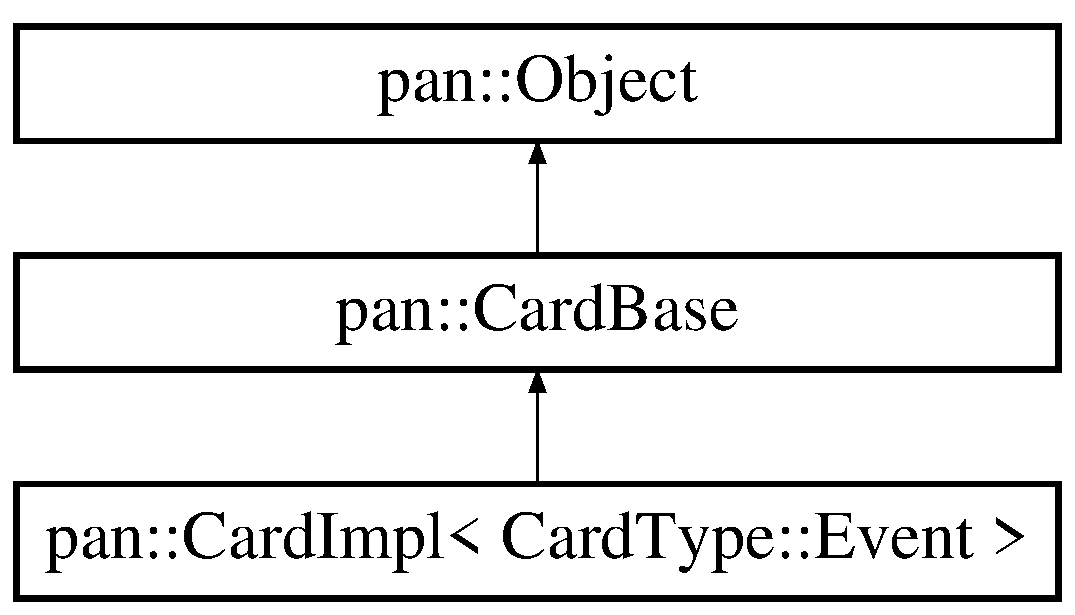
\includegraphics[height=3.000000cm]{classpan_1_1_card_impl_3_01_card_type_1_1_event_01_4}
\end{center}
\end{figure}
\subsection*{Public Member Functions}
\begin{DoxyCompactItemize}
\item 
\hyperlink{classpan_1_1_card_impl_3_01_card_type_1_1_event_01_4_ad31a4637fd5d1c1c2aac120109b3c4e8}{Card\+Impl} (\hyperlink{namespacepan_a9221a73b34e019e6b8fe6f84e6417513}{Event\+Type} \hyperlink{classpan_1_1_card_impl_3_01_card_type_1_1_event_01_4_a575f1457eebafca8f0c975bdec2258e2}{event\+Type})
\item 
\hyperlink{classpan_1_1_card_impl_3_01_card_type_1_1_event_01_4_a57a0df69033b57c0476c3d58599cb079}{$\sim$\+Card\+Impl} ()=default
\item 
std\+::string \hyperlink{classpan_1_1_card_impl_3_01_card_type_1_1_event_01_4_aa5c7d2729e0bfb141a0d8487a590a580}{description} () const
\item 
bool \hyperlink{classpan_1_1_card_impl_3_01_card_type_1_1_event_01_4_af97461f7279365bc5bd0c0490a51b13f}{operator==} (const \hyperlink{classpan_1_1_card_impl}{Card\+Impl} \&) const
\item 
bool \hyperlink{classpan_1_1_card_impl_3_01_card_type_1_1_event_01_4_aac9dd96956122fdb62852408e86d767e}{operator!=} (const \hyperlink{classpan_1_1_card_impl}{Card\+Impl} \&) const
\end{DoxyCompactItemize}
\subsection*{Public Attributes}
\begin{DoxyCompactItemize}
\item 
const \hyperlink{namespacepan_a9221a73b34e019e6b8fe6f84e6417513}{Event\+Type} \hyperlink{classpan_1_1_card_impl_3_01_card_type_1_1_event_01_4_a575f1457eebafca8f0c975bdec2258e2}{event\+Type}
\end{DoxyCompactItemize}
\subsection*{Friends}
\begin{DoxyCompactItemize}
\item 
class \hyperlink{classpan_1_1_card_impl_3_01_card_type_1_1_event_01_4_ac98d07dd8f7b70e16ccb9a01abf56b9c}{boost\+::serialization\+::access}
\end{DoxyCompactItemize}


\subsection{Detailed Description}
\subsubsection*{template$<$$>$\newline
class pan\+::\+Card\+Impl$<$ Card\+Type\+::\+Event $>$}

Represents the Event Card entity. 

\begin{DoxyAuthor}{Author}
Hrachya Hakobyan 
\end{DoxyAuthor}


\subsection{Constructor \& Destructor Documentation}
\mbox{\Hypertarget{classpan_1_1_card_impl_3_01_card_type_1_1_event_01_4_ad31a4637fd5d1c1c2aac120109b3c4e8}\label{classpan_1_1_card_impl_3_01_card_type_1_1_event_01_4_ad31a4637fd5d1c1c2aac120109b3c4e8}} 
\index{pan\+::\+Card\+Impl$<$ Card\+Type\+::\+Event $>$@{pan\+::\+Card\+Impl$<$ Card\+Type\+::\+Event $>$}!Card\+Impl@{Card\+Impl}}
\index{Card\+Impl@{Card\+Impl}!pan\+::\+Card\+Impl$<$ Card\+Type\+::\+Event $>$@{pan\+::\+Card\+Impl$<$ Card\+Type\+::\+Event $>$}}
\subsubsection{\texorpdfstring{Card\+Impl()}{CardImpl()}}
{\footnotesize\ttfamily \hyperlink{classpan_1_1_card_impl}{pan\+::\+Card\+Impl}$<$ \hyperlink{namespacepan_a1f7350bfd0421afeabe9fa95c16fa811aa4ecfc70574394990cf17bd83df499f7}{Card\+Type\+::\+Event} $>$\+::\hyperlink{classpan_1_1_card_impl}{Card\+Impl} (\begin{DoxyParamCaption}\item[{\hyperlink{namespacepan_a9221a73b34e019e6b8fe6f84e6417513}{Event\+Type}}]{event\+Type }\end{DoxyParamCaption})}

\mbox{\Hypertarget{classpan_1_1_card_impl_3_01_card_type_1_1_event_01_4_a57a0df69033b57c0476c3d58599cb079}\label{classpan_1_1_card_impl_3_01_card_type_1_1_event_01_4_a57a0df69033b57c0476c3d58599cb079}} 
\index{pan\+::\+Card\+Impl$<$ Card\+Type\+::\+Event $>$@{pan\+::\+Card\+Impl$<$ Card\+Type\+::\+Event $>$}!````~Card\+Impl@{$\sim$\+Card\+Impl}}
\index{````~Card\+Impl@{$\sim$\+Card\+Impl}!pan\+::\+Card\+Impl$<$ Card\+Type\+::\+Event $>$@{pan\+::\+Card\+Impl$<$ Card\+Type\+::\+Event $>$}}
\subsubsection{\texorpdfstring{$\sim$\+Card\+Impl()}{~CardImpl()}}
{\footnotesize\ttfamily \hyperlink{classpan_1_1_card_impl}{pan\+::\+Card\+Impl}$<$ \hyperlink{namespacepan_a1f7350bfd0421afeabe9fa95c16fa811aa4ecfc70574394990cf17bd83df499f7}{Card\+Type\+::\+Event} $>$\+::$\sim$\hyperlink{classpan_1_1_card_impl}{Card\+Impl} (\begin{DoxyParamCaption}{ }\end{DoxyParamCaption})\hspace{0.3cm}{\ttfamily [default]}}



\subsection{Member Function Documentation}
\mbox{\Hypertarget{classpan_1_1_card_impl_3_01_card_type_1_1_event_01_4_aa5c7d2729e0bfb141a0d8487a590a580}\label{classpan_1_1_card_impl_3_01_card_type_1_1_event_01_4_aa5c7d2729e0bfb141a0d8487a590a580}} 
\index{pan\+::\+Card\+Impl$<$ Card\+Type\+::\+Event $>$@{pan\+::\+Card\+Impl$<$ Card\+Type\+::\+Event $>$}!description@{description}}
\index{description@{description}!pan\+::\+Card\+Impl$<$ Card\+Type\+::\+Event $>$@{pan\+::\+Card\+Impl$<$ Card\+Type\+::\+Event $>$}}
\subsubsection{\texorpdfstring{description()}{description()}}
{\footnotesize\ttfamily std\+::string \hyperlink{classpan_1_1_card_impl}{pan\+::\+Card\+Impl}$<$ \hyperlink{namespacepan_a1f7350bfd0421afeabe9fa95c16fa811aa4ecfc70574394990cf17bd83df499f7}{Card\+Type\+::\+Event} $>$\+::description (\begin{DoxyParamCaption}{ }\end{DoxyParamCaption}) const\hspace{0.3cm}{\ttfamily [inline]}, {\ttfamily [virtual]}}



Reimplemented from \hyperlink{classpan_1_1_card_base_ad004c502404a958eaf4ecae7e73cc8cf}{pan\+::\+Card\+Base}.

\mbox{\Hypertarget{classpan_1_1_card_impl_3_01_card_type_1_1_event_01_4_aac9dd96956122fdb62852408e86d767e}\label{classpan_1_1_card_impl_3_01_card_type_1_1_event_01_4_aac9dd96956122fdb62852408e86d767e}} 
\index{pan\+::\+Card\+Impl$<$ Card\+Type\+::\+Event $>$@{pan\+::\+Card\+Impl$<$ Card\+Type\+::\+Event $>$}!operator"!=@{operator"!=}}
\index{operator"!=@{operator"!=}!pan\+::\+Card\+Impl$<$ Card\+Type\+::\+Event $>$@{pan\+::\+Card\+Impl$<$ Card\+Type\+::\+Event $>$}}
\subsubsection{\texorpdfstring{operator"!=()}{operator!=()}}
{\footnotesize\ttfamily bool \hyperlink{classpan_1_1_card_impl}{pan\+::\+Card\+Impl}$<$ \hyperlink{namespacepan_a1f7350bfd0421afeabe9fa95c16fa811aa4ecfc70574394990cf17bd83df499f7}{Card\+Type\+::\+Event} $>$\+::operator!= (\begin{DoxyParamCaption}\item[{const \hyperlink{classpan_1_1_card_impl}{Card\+Impl}$<$ \hyperlink{namespacepan_a1f7350bfd0421afeabe9fa95c16fa811aa4ecfc70574394990cf17bd83df499f7}{Card\+Type\+::\+Event} $>$ \&}]{o }\end{DoxyParamCaption}) const\hspace{0.3cm}{\ttfamily [inline]}}

\mbox{\Hypertarget{classpan_1_1_card_impl_3_01_card_type_1_1_event_01_4_af97461f7279365bc5bd0c0490a51b13f}\label{classpan_1_1_card_impl_3_01_card_type_1_1_event_01_4_af97461f7279365bc5bd0c0490a51b13f}} 
\index{pan\+::\+Card\+Impl$<$ Card\+Type\+::\+Event $>$@{pan\+::\+Card\+Impl$<$ Card\+Type\+::\+Event $>$}!operator==@{operator==}}
\index{operator==@{operator==}!pan\+::\+Card\+Impl$<$ Card\+Type\+::\+Event $>$@{pan\+::\+Card\+Impl$<$ Card\+Type\+::\+Event $>$}}
\subsubsection{\texorpdfstring{operator==()}{operator==()}}
{\footnotesize\ttfamily bool \hyperlink{classpan_1_1_card_impl}{pan\+::\+Card\+Impl}$<$ \hyperlink{namespacepan_a1f7350bfd0421afeabe9fa95c16fa811aa4ecfc70574394990cf17bd83df499f7}{Card\+Type\+::\+Event} $>$\+::operator== (\begin{DoxyParamCaption}\item[{const \hyperlink{classpan_1_1_card_impl}{Card\+Impl}$<$ \hyperlink{namespacepan_a1f7350bfd0421afeabe9fa95c16fa811aa4ecfc70574394990cf17bd83df499f7}{Card\+Type\+::\+Event} $>$ \&}]{o }\end{DoxyParamCaption}) const\hspace{0.3cm}{\ttfamily [inline]}}



\subsection{Friends And Related Function Documentation}
\mbox{\Hypertarget{classpan_1_1_card_impl_3_01_card_type_1_1_event_01_4_ac98d07dd8f7b70e16ccb9a01abf56b9c}\label{classpan_1_1_card_impl_3_01_card_type_1_1_event_01_4_ac98d07dd8f7b70e16ccb9a01abf56b9c}} 
\index{pan\+::\+Card\+Impl$<$ Card\+Type\+::\+Event $>$@{pan\+::\+Card\+Impl$<$ Card\+Type\+::\+Event $>$}!boost\+::serialization\+::access@{boost\+::serialization\+::access}}
\index{boost\+::serialization\+::access@{boost\+::serialization\+::access}!pan\+::\+Card\+Impl$<$ Card\+Type\+::\+Event $>$@{pan\+::\+Card\+Impl$<$ Card\+Type\+::\+Event $>$}}
\subsubsection{\texorpdfstring{boost\+::serialization\+::access}{boost::serialization::access}}
{\footnotesize\ttfamily friend class boost\+::serialization\+::access\hspace{0.3cm}{\ttfamily [friend]}}



\subsection{Member Data Documentation}
\mbox{\Hypertarget{classpan_1_1_card_impl_3_01_card_type_1_1_event_01_4_a575f1457eebafca8f0c975bdec2258e2}\label{classpan_1_1_card_impl_3_01_card_type_1_1_event_01_4_a575f1457eebafca8f0c975bdec2258e2}} 
\index{pan\+::\+Card\+Impl$<$ Card\+Type\+::\+Event $>$@{pan\+::\+Card\+Impl$<$ Card\+Type\+::\+Event $>$}!event\+Type@{event\+Type}}
\index{event\+Type@{event\+Type}!pan\+::\+Card\+Impl$<$ Card\+Type\+::\+Event $>$@{pan\+::\+Card\+Impl$<$ Card\+Type\+::\+Event $>$}}
\subsubsection{\texorpdfstring{event\+Type}{eventType}}
{\footnotesize\ttfamily const \hyperlink{namespacepan_a9221a73b34e019e6b8fe6f84e6417513}{Event\+Type} \hyperlink{classpan_1_1_card_impl}{pan\+::\+Card\+Impl}$<$ \hyperlink{namespacepan_a1f7350bfd0421afeabe9fa95c16fa811aa4ecfc70574394990cf17bd83df499f7}{Card\+Type\+::\+Event} $>$\+::event\+Type}



The documentation for this class was generated from the following files\+:\begin{DoxyCompactItemize}
\item 
\hyperlink{_event_card_8h}{Event\+Card.\+h}\item 
\hyperlink{_event_card_8cpp}{Event\+Card.\+cpp}\end{DoxyCompactItemize}

\hypertarget{classpan_1_1_card_impl_3_01_card_type_1_1_infection_01_4}{}\section{pan\+:\+:Card\+Impl$<$ Card\+Type\+:\+:Infection $>$ Class Template Reference}
\label{classpan_1_1_card_impl_3_01_card_type_1_1_infection_01_4}\index{pan\+::\+Card\+Impl$<$ Card\+Type\+::\+Infection $>$@{pan\+::\+Card\+Impl$<$ Card\+Type\+::\+Infection $>$}}


Represents the Infection card entity.  




{\ttfamily \#include $<$Infection\+Card.\+h$>$}

Inheritance diagram for pan\+:\+:Card\+Impl$<$ Card\+Type\+:\+:Infection $>$\+:\begin{figure}[H]
\begin{center}
\leavevmode
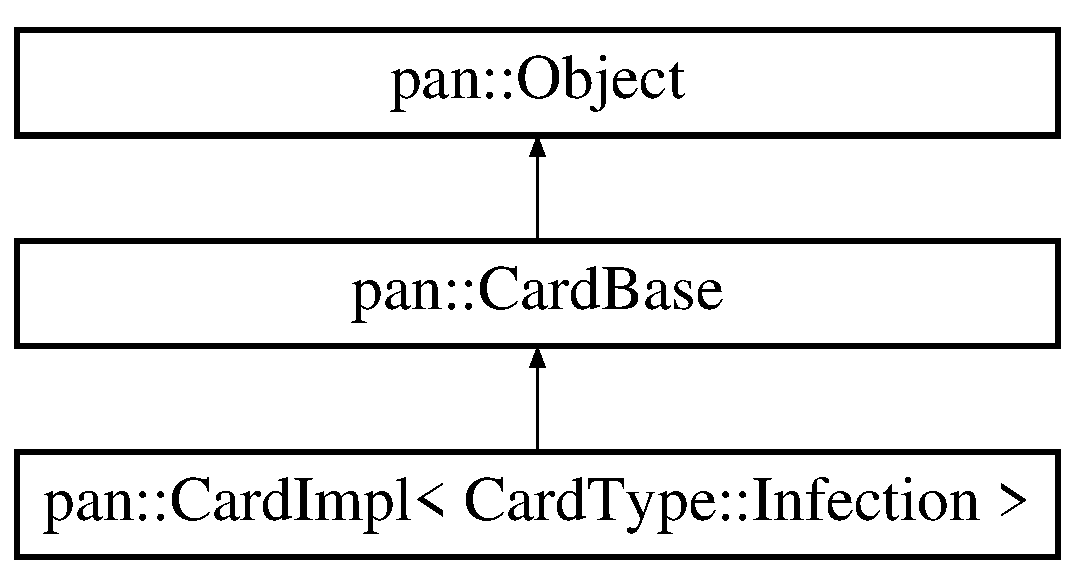
\includegraphics[height=3.000000cm]{classpan_1_1_card_impl_3_01_card_type_1_1_infection_01_4}
\end{center}
\end{figure}
\subsection*{Public Member Functions}
\begin{DoxyCompactItemize}
\item 
\hyperlink{classpan_1_1_card_impl_3_01_card_type_1_1_infection_01_4_a949201ae0814de52ad3c126a189b0f74}{Card\+Impl} (\hyperlink{namespacepan_afaed28aa6603153dcc062a028602d697}{City\+Index} index)
\item 
\hyperlink{classpan_1_1_card_impl_3_01_card_type_1_1_infection_01_4_ae3fe3d61f83d4f5a79a08d0dad43b9c2}{$\sim$\+Card\+Impl} ()=default
\item 
std\+::string \hyperlink{classpan_1_1_card_impl_3_01_card_type_1_1_infection_01_4_a5e31904120b655ce59633433a4d4c17c}{description} () const
\item 
bool \hyperlink{classpan_1_1_card_impl_3_01_card_type_1_1_infection_01_4_a868c2a678649606cb485ab66e47f0eb2}{operator==} (const \hyperlink{classpan_1_1_card_impl}{Card\+Impl} \&) const
\item 
bool \hyperlink{classpan_1_1_card_impl_3_01_card_type_1_1_infection_01_4_ae372e0ba38c16ccb791c0f951731f056}{operator!=} (const \hyperlink{classpan_1_1_card_impl}{Card\+Impl} \&) const
\end{DoxyCompactItemize}
\subsection*{Public Attributes}
\begin{DoxyCompactItemize}
\item 
const \hyperlink{namespacepan_afaed28aa6603153dcc062a028602d697}{City\+Index} \hyperlink{classpan_1_1_card_impl_3_01_card_type_1_1_infection_01_4_a6997050312a4c6d9e431e445862e5ed5}{city\+Index}
\end{DoxyCompactItemize}
\subsection*{Friends}
\begin{DoxyCompactItemize}
\item 
class \hyperlink{classpan_1_1_card_impl_3_01_card_type_1_1_infection_01_4_ac98d07dd8f7b70e16ccb9a01abf56b9c}{boost\+::serialization\+::access}
\end{DoxyCompactItemize}


\subsection{Detailed Description}
\subsubsection*{template$<$$>$\newline
class pan\+::\+Card\+Impl$<$ Card\+Type\+::\+Infection $>$}

Represents the Infection card entity. 

\begin{DoxyAuthor}{Author}
Hrachya Hakobyan 
\end{DoxyAuthor}


\subsection{Constructor \& Destructor Documentation}
\mbox{\Hypertarget{classpan_1_1_card_impl_3_01_card_type_1_1_infection_01_4_a949201ae0814de52ad3c126a189b0f74}\label{classpan_1_1_card_impl_3_01_card_type_1_1_infection_01_4_a949201ae0814de52ad3c126a189b0f74}} 
\index{pan\+::\+Card\+Impl$<$ Card\+Type\+::\+Infection $>$@{pan\+::\+Card\+Impl$<$ Card\+Type\+::\+Infection $>$}!Card\+Impl@{Card\+Impl}}
\index{Card\+Impl@{Card\+Impl}!pan\+::\+Card\+Impl$<$ Card\+Type\+::\+Infection $>$@{pan\+::\+Card\+Impl$<$ Card\+Type\+::\+Infection $>$}}
\subsubsection{\texorpdfstring{Card\+Impl()}{CardImpl()}}
{\footnotesize\ttfamily \hyperlink{classpan_1_1_card_impl}{pan\+::\+Card\+Impl}$<$ \hyperlink{namespacepan_a1f7350bfd0421afeabe9fa95c16fa811af0ddc0838281faf6d55e2cf840a2a8ef}{Card\+Type\+::\+Infection} $>$\+::\hyperlink{classpan_1_1_card_impl}{Card\+Impl} (\begin{DoxyParamCaption}\item[{\hyperlink{namespacepan_afaed28aa6603153dcc062a028602d697}{City\+Index}}]{index }\end{DoxyParamCaption})}

\mbox{\Hypertarget{classpan_1_1_card_impl_3_01_card_type_1_1_infection_01_4_ae3fe3d61f83d4f5a79a08d0dad43b9c2}\label{classpan_1_1_card_impl_3_01_card_type_1_1_infection_01_4_ae3fe3d61f83d4f5a79a08d0dad43b9c2}} 
\index{pan\+::\+Card\+Impl$<$ Card\+Type\+::\+Infection $>$@{pan\+::\+Card\+Impl$<$ Card\+Type\+::\+Infection $>$}!````~Card\+Impl@{$\sim$\+Card\+Impl}}
\index{````~Card\+Impl@{$\sim$\+Card\+Impl}!pan\+::\+Card\+Impl$<$ Card\+Type\+::\+Infection $>$@{pan\+::\+Card\+Impl$<$ Card\+Type\+::\+Infection $>$}}
\subsubsection{\texorpdfstring{$\sim$\+Card\+Impl()}{~CardImpl()}}
{\footnotesize\ttfamily \hyperlink{classpan_1_1_card_impl}{pan\+::\+Card\+Impl}$<$ \hyperlink{namespacepan_a1f7350bfd0421afeabe9fa95c16fa811af0ddc0838281faf6d55e2cf840a2a8ef}{Card\+Type\+::\+Infection} $>$\+::$\sim$\hyperlink{classpan_1_1_card_impl}{Card\+Impl} (\begin{DoxyParamCaption}{ }\end{DoxyParamCaption})\hspace{0.3cm}{\ttfamily [default]}}



\subsection{Member Function Documentation}
\mbox{\Hypertarget{classpan_1_1_card_impl_3_01_card_type_1_1_infection_01_4_a5e31904120b655ce59633433a4d4c17c}\label{classpan_1_1_card_impl_3_01_card_type_1_1_infection_01_4_a5e31904120b655ce59633433a4d4c17c}} 
\index{pan\+::\+Card\+Impl$<$ Card\+Type\+::\+Infection $>$@{pan\+::\+Card\+Impl$<$ Card\+Type\+::\+Infection $>$}!description@{description}}
\index{description@{description}!pan\+::\+Card\+Impl$<$ Card\+Type\+::\+Infection $>$@{pan\+::\+Card\+Impl$<$ Card\+Type\+::\+Infection $>$}}
\subsubsection{\texorpdfstring{description()}{description()}}
{\footnotesize\ttfamily std\+::string \hyperlink{classpan_1_1_card_impl}{pan\+::\+Card\+Impl}$<$ \hyperlink{namespacepan_a1f7350bfd0421afeabe9fa95c16fa811af0ddc0838281faf6d55e2cf840a2a8ef}{Card\+Type\+::\+Infection} $>$\+::description (\begin{DoxyParamCaption}{ }\end{DoxyParamCaption}) const\hspace{0.3cm}{\ttfamily [inline]}, {\ttfamily [virtual]}}



Reimplemented from \hyperlink{classpan_1_1_card_base_ad004c502404a958eaf4ecae7e73cc8cf}{pan\+::\+Card\+Base}.

\mbox{\Hypertarget{classpan_1_1_card_impl_3_01_card_type_1_1_infection_01_4_ae372e0ba38c16ccb791c0f951731f056}\label{classpan_1_1_card_impl_3_01_card_type_1_1_infection_01_4_ae372e0ba38c16ccb791c0f951731f056}} 
\index{pan\+::\+Card\+Impl$<$ Card\+Type\+::\+Infection $>$@{pan\+::\+Card\+Impl$<$ Card\+Type\+::\+Infection $>$}!operator"!=@{operator"!=}}
\index{operator"!=@{operator"!=}!pan\+::\+Card\+Impl$<$ Card\+Type\+::\+Infection $>$@{pan\+::\+Card\+Impl$<$ Card\+Type\+::\+Infection $>$}}
\subsubsection{\texorpdfstring{operator"!=()}{operator!=()}}
{\footnotesize\ttfamily bool \hyperlink{classpan_1_1_card_impl}{pan\+::\+Card\+Impl}$<$ \hyperlink{namespacepan_a1f7350bfd0421afeabe9fa95c16fa811af0ddc0838281faf6d55e2cf840a2a8ef}{Card\+Type\+::\+Infection} $>$\+::operator!= (\begin{DoxyParamCaption}\item[{const \hyperlink{classpan_1_1_card_impl}{Card\+Impl}$<$ \hyperlink{namespacepan_a1f7350bfd0421afeabe9fa95c16fa811af0ddc0838281faf6d55e2cf840a2a8ef}{Card\+Type\+::\+Infection} $>$ \&}]{o }\end{DoxyParamCaption}) const\hspace{0.3cm}{\ttfamily [inline]}}

\mbox{\Hypertarget{classpan_1_1_card_impl_3_01_card_type_1_1_infection_01_4_a868c2a678649606cb485ab66e47f0eb2}\label{classpan_1_1_card_impl_3_01_card_type_1_1_infection_01_4_a868c2a678649606cb485ab66e47f0eb2}} 
\index{pan\+::\+Card\+Impl$<$ Card\+Type\+::\+Infection $>$@{pan\+::\+Card\+Impl$<$ Card\+Type\+::\+Infection $>$}!operator==@{operator==}}
\index{operator==@{operator==}!pan\+::\+Card\+Impl$<$ Card\+Type\+::\+Infection $>$@{pan\+::\+Card\+Impl$<$ Card\+Type\+::\+Infection $>$}}
\subsubsection{\texorpdfstring{operator==()}{operator==()}}
{\footnotesize\ttfamily bool \hyperlink{classpan_1_1_card_impl}{pan\+::\+Card\+Impl}$<$ \hyperlink{namespacepan_a1f7350bfd0421afeabe9fa95c16fa811af0ddc0838281faf6d55e2cf840a2a8ef}{Card\+Type\+::\+Infection} $>$\+::operator== (\begin{DoxyParamCaption}\item[{const \hyperlink{classpan_1_1_card_impl}{Card\+Impl}$<$ \hyperlink{namespacepan_a1f7350bfd0421afeabe9fa95c16fa811af0ddc0838281faf6d55e2cf840a2a8ef}{Card\+Type\+::\+Infection} $>$ \&}]{o }\end{DoxyParamCaption}) const\hspace{0.3cm}{\ttfamily [inline]}}



\subsection{Friends And Related Function Documentation}
\mbox{\Hypertarget{classpan_1_1_card_impl_3_01_card_type_1_1_infection_01_4_ac98d07dd8f7b70e16ccb9a01abf56b9c}\label{classpan_1_1_card_impl_3_01_card_type_1_1_infection_01_4_ac98d07dd8f7b70e16ccb9a01abf56b9c}} 
\index{pan\+::\+Card\+Impl$<$ Card\+Type\+::\+Infection $>$@{pan\+::\+Card\+Impl$<$ Card\+Type\+::\+Infection $>$}!boost\+::serialization\+::access@{boost\+::serialization\+::access}}
\index{boost\+::serialization\+::access@{boost\+::serialization\+::access}!pan\+::\+Card\+Impl$<$ Card\+Type\+::\+Infection $>$@{pan\+::\+Card\+Impl$<$ Card\+Type\+::\+Infection $>$}}
\subsubsection{\texorpdfstring{boost\+::serialization\+::access}{boost::serialization::access}}
{\footnotesize\ttfamily friend class boost\+::serialization\+::access\hspace{0.3cm}{\ttfamily [friend]}}



\subsection{Member Data Documentation}
\mbox{\Hypertarget{classpan_1_1_card_impl_3_01_card_type_1_1_infection_01_4_a6997050312a4c6d9e431e445862e5ed5}\label{classpan_1_1_card_impl_3_01_card_type_1_1_infection_01_4_a6997050312a4c6d9e431e445862e5ed5}} 
\index{pan\+::\+Card\+Impl$<$ Card\+Type\+::\+Infection $>$@{pan\+::\+Card\+Impl$<$ Card\+Type\+::\+Infection $>$}!city\+Index@{city\+Index}}
\index{city\+Index@{city\+Index}!pan\+::\+Card\+Impl$<$ Card\+Type\+::\+Infection $>$@{pan\+::\+Card\+Impl$<$ Card\+Type\+::\+Infection $>$}}
\subsubsection{\texorpdfstring{city\+Index}{cityIndex}}
{\footnotesize\ttfamily const \hyperlink{namespacepan_afaed28aa6603153dcc062a028602d697}{City\+Index} \hyperlink{classpan_1_1_card_impl}{pan\+::\+Card\+Impl}$<$ \hyperlink{namespacepan_a1f7350bfd0421afeabe9fa95c16fa811af0ddc0838281faf6d55e2cf840a2a8ef}{Card\+Type\+::\+Infection} $>$\+::city\+Index}



The documentation for this class was generated from the following files\+:\begin{DoxyCompactItemize}
\item 
\hyperlink{_infection_card_8h}{Infection\+Card.\+h}\item 
\hyperlink{_infection_card_8cpp}{Infection\+Card.\+cpp}\end{DoxyCompactItemize}

\hypertarget{classpan_1_1_charter_flight}{}\section{pan\+:\+:Charter\+Flight Class Reference}
\label{classpan_1_1_charter_flight}\index{pan\+::\+Charter\+Flight@{pan\+::\+Charter\+Flight}}


Class representing a charter flight action.  




{\ttfamily \#include $<$Charter\+Flight.\+h$>$}

Inheritance diagram for pan\+:\+:Charter\+Flight\+:\begin{figure}[H]
\begin{center}
\leavevmode
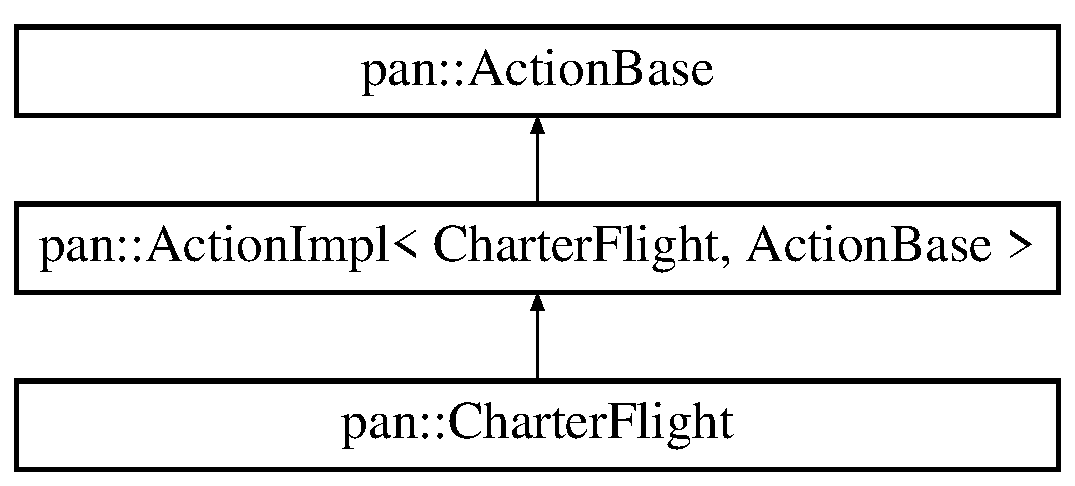
\includegraphics[height=3.000000cm]{classpan_1_1_charter_flight}
\end{center}
\end{figure}
\subsection*{Public Member Functions}
\begin{DoxyCompactItemize}
\item 
\hyperlink{classpan_1_1_charter_flight_a7e1ae3b2d535c17702106f6bb18d19bc}{Charter\+Flight} (\hyperlink{namespacepan_a0cdabf874fbf1bb3a1f0152d108c2909}{Player\+Index} \hyperlink{classpan_1_1_charter_flight_a36cd9c4ffde7f07b1d187fddc00638d5}{player}, \hyperlink{namespacepan_afaed28aa6603153dcc062a028602d697}{City\+Index} city)
\end{DoxyCompactItemize}
\subsection*{Public Attributes}
\begin{DoxyCompactItemize}
\item 
\hyperlink{namespacepan_a0cdabf874fbf1bb3a1f0152d108c2909}{Player\+Index} \hyperlink{classpan_1_1_charter_flight_a36cd9c4ffde7f07b1d187fddc00638d5}{player}
\item 
\hyperlink{namespacepan_afaed28aa6603153dcc062a028602d697}{City\+Index} \hyperlink{classpan_1_1_charter_flight_a21a435071a78d4a57670fca2f5234b3f}{target\+City}
\end{DoxyCompactItemize}


\subsection{Detailed Description}
Class representing a charter flight action. 

\begin{DoxyAuthor}{Author}
Hrachya Hakobyan 
\end{DoxyAuthor}


\subsection{Constructor \& Destructor Documentation}
\mbox{\Hypertarget{classpan_1_1_charter_flight_a7e1ae3b2d535c17702106f6bb18d19bc}\label{classpan_1_1_charter_flight_a7e1ae3b2d535c17702106f6bb18d19bc}} 
\index{pan\+::\+Charter\+Flight@{pan\+::\+Charter\+Flight}!Charter\+Flight@{Charter\+Flight}}
\index{Charter\+Flight@{Charter\+Flight}!pan\+::\+Charter\+Flight@{pan\+::\+Charter\+Flight}}
\subsubsection{\texorpdfstring{Charter\+Flight()}{CharterFlight()}}
{\footnotesize\ttfamily pan\+::\+Charter\+Flight\+::\+Charter\+Flight (\begin{DoxyParamCaption}\item[{\hyperlink{namespacepan_a0cdabf874fbf1bb3a1f0152d108c2909}{Player\+Index}}]{player,  }\item[{\hyperlink{namespacepan_afaed28aa6603153dcc062a028602d697}{City\+Index}}]{city }\end{DoxyParamCaption})}



\subsection{Member Data Documentation}
\mbox{\Hypertarget{classpan_1_1_charter_flight_a36cd9c4ffde7f07b1d187fddc00638d5}\label{classpan_1_1_charter_flight_a36cd9c4ffde7f07b1d187fddc00638d5}} 
\index{pan\+::\+Charter\+Flight@{pan\+::\+Charter\+Flight}!player@{player}}
\index{player@{player}!pan\+::\+Charter\+Flight@{pan\+::\+Charter\+Flight}}
\subsubsection{\texorpdfstring{player}{player}}
{\footnotesize\ttfamily \hyperlink{namespacepan_a0cdabf874fbf1bb3a1f0152d108c2909}{Player\+Index} pan\+::\+Charter\+Flight\+::player}

\mbox{\Hypertarget{classpan_1_1_charter_flight_a21a435071a78d4a57670fca2f5234b3f}\label{classpan_1_1_charter_flight_a21a435071a78d4a57670fca2f5234b3f}} 
\index{pan\+::\+Charter\+Flight@{pan\+::\+Charter\+Flight}!target\+City@{target\+City}}
\index{target\+City@{target\+City}!pan\+::\+Charter\+Flight@{pan\+::\+Charter\+Flight}}
\subsubsection{\texorpdfstring{target\+City}{targetCity}}
{\footnotesize\ttfamily \hyperlink{namespacepan_afaed28aa6603153dcc062a028602d697}{City\+Index} pan\+::\+Charter\+Flight\+::target\+City}



The documentation for this class was generated from the following files\+:\begin{DoxyCompactItemize}
\item 
\hyperlink{_charter_flight_8h}{Charter\+Flight.\+h}\item 
\hyperlink{_charter_flight_8cpp}{Charter\+Flight.\+cpp}\end{DoxyCompactItemize}

\hypertarget{classpan_1_1_city}{}\section{pan\+:\+:City Class Reference}
\label{classpan_1_1_city}\index{pan\+::\+City@{pan\+::\+City}}


Represents a single city on the map. Is default constructible, copyable and assignable to allow usage with containers.  




{\ttfamily \#include $<$City.\+h$>$}

Inheritance diagram for pan\+:\+:City\+:\begin{figure}[H]
\begin{center}
\leavevmode
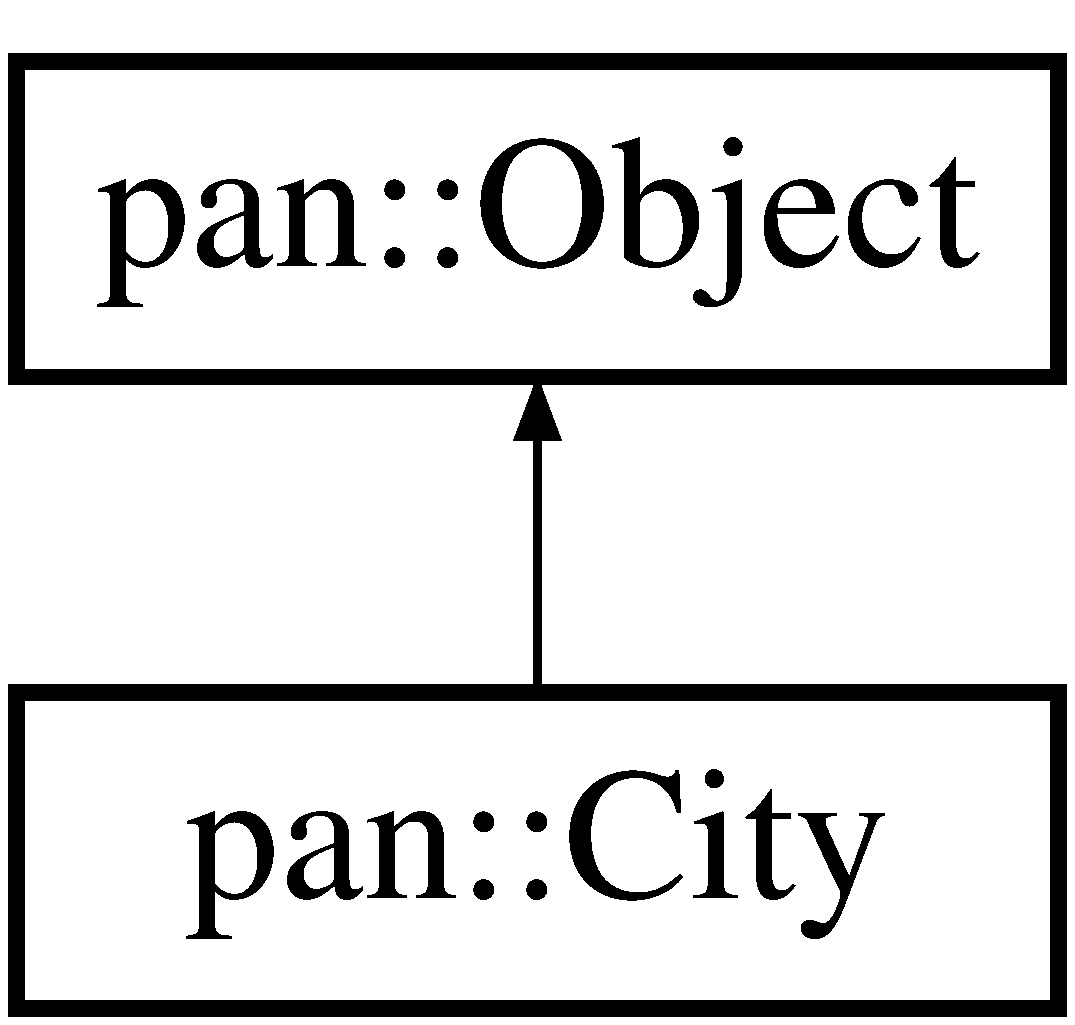
\includegraphics[height=2.000000cm]{classpan_1_1_city}
\end{center}
\end{figure}
\subsection*{Public Member Functions}
\begin{DoxyCompactItemize}
\item 
\hyperlink{classpan_1_1_city_abf8a8407beecfc243044a6928960dc25}{City} ()
\item 
\hyperlink{classpan_1_1_city_a0a167d009ec26423e3f64a952e6f5835}{City} (const std\+::string \&name, unsigned int \hyperlink{classpan_1_1_city_aedd352c6f6ecaf1c78184189cef035b7}{population}=0)
\item 
\hyperlink{classpan_1_1_city_ae007f3169e698aa000bd8d20de1e278b}{City} (const std\+::string \&name, unsigned int \hyperlink{classpan_1_1_city_aedd352c6f6ecaf1c78184189cef035b7}{population}, double xpos, double ypos)
\item 
\hyperlink{classpan_1_1_city_ae7eeaa8d62dc361a7ad7be657cc41e69}{City} (const \hyperlink{classpan_1_1_city}{City} \&)
\item 
\hyperlink{classpan_1_1_city_a77b79e8d2ae5e9fa6ae37d290c87df2f}{City} (\hyperlink{classpan_1_1_city}{City} \&\&o)
\item 
\hyperlink{classpan_1_1_city}{City} \& \hyperlink{classpan_1_1_city_af289409b1c1d687cc74b163dd15b4133}{operator=} (const \hyperlink{classpan_1_1_city}{City} \&)
\item 
\hyperlink{classpan_1_1_city}{City} \& \hyperlink{classpan_1_1_city_a10109e483fc579bca4124135a238a7e3}{operator=} (\hyperlink{classpan_1_1_city}{City} \&\&)
\item 
\hyperlink{classpan_1_1_city_a5cec0ac09c157ca262c61a1fbb7debf3}{$\sim$\+City} ()=default
\item 
bool \hyperlink{classpan_1_1_city_ac43e794b9736734744c81d28387a4d26}{operator==} (const \hyperlink{classpan_1_1_city}{City} \&other) const
\item 
bool \hyperlink{classpan_1_1_city_a5fefdda50088576ad882402a266fded8}{operator!=} (const \hyperlink{classpan_1_1_city}{City} \&other) const
\item 
std\+::string \hyperlink{classpan_1_1_city_a0232df988764b10f50570e335e8237c2}{description} () const
\item 
std\+::size\+\_\+t \hyperlink{classpan_1_1_city_a0267d8dd3cc41d23ceabe4a6a8172df5}{player\+Count} () const
\item 
const std\+::set$<$ \hyperlink{namespacepan_a0cdabf874fbf1bb3a1f0152d108c2909}{Player\+Index} $>$ \& \hyperlink{classpan_1_1_city_af141a83daaa0521bbad892ba9c7fd6c3}{get\+Players} () const
\item 
bool \hyperlink{classpan_1_1_city_af548c54d6e134c72c6bb9b2ab895f7d5}{contains\+Player} (\hyperlink{namespacepan_a0cdabf874fbf1bb3a1f0152d108c2909}{Player\+Index} p) const
\item 
void \hyperlink{classpan_1_1_city_aef9a86d5ddb998226127e21df91a7589}{add\+Player} (\hyperlink{namespacepan_a0cdabf874fbf1bb3a1f0152d108c2909}{Player\+Index} p)
\item 
void \hyperlink{classpan_1_1_city_aa3ed9dcde255c83466431f6b55031e9d}{remove\+Player} (\hyperlink{namespacepan_a0cdabf874fbf1bb3a1f0152d108c2909}{Player\+Index} p)
\item 
const std\+::string \& \hyperlink{classpan_1_1_city_a5b6f8e81d190dcddd6d78445cba7f694}{get\+Name} () const
\item 
void \hyperlink{classpan_1_1_city_a9a25b8843ae24c9bbe36a818aa29a9d5}{set\+Name} (const std\+::string \&name)
\item 
std\+::size\+\_\+t \hyperlink{classpan_1_1_city_ae6c690c21186c5531eb5fc7a314e8e2d}{get\+Cubes} (\hyperlink{namespacepan_a48851b51b0aef3f0e1be80df5031d9d7}{Disease\+Type} r) const
\item 
void \hyperlink{classpan_1_1_city_abd77b16cbb277ff3dd9699e4e79ed1d5}{set\+Cubes} (\hyperlink{namespacepan_a48851b51b0aef3f0e1be80df5031d9d7}{Disease\+Type} r, std\+::size\+\_\+t cubes)
\item 
{\footnotesize template$<$class Archive $>$ }\\void \hyperlink{classpan_1_1_city_a712b0f8a3f35f7caf3f3b8795a89658b}{serialize} (Archive \&ar, const unsigned int)
\end{DoxyCompactItemize}
\subsection*{Public Attributes}
\begin{DoxyCompactItemize}
\item 
unsigned int \hyperlink{classpan_1_1_city_aedd352c6f6ecaf1c78184189cef035b7}{population} = 0
\item 
bool \hyperlink{classpan_1_1_city_ae278568277b94033909dbf31ad8843ff}{research\+Station} = false
\end{DoxyCompactItemize}
\subsection*{Friends}
\begin{DoxyCompactItemize}
\item 
class \hyperlink{classpan_1_1_city_ac98d07dd8f7b70e16ccb9a01abf56b9c}{boost\+::serialization\+::access}
\end{DoxyCompactItemize}


\subsection{Detailed Description}
Represents a single city on the map. Is default constructible, copyable and assignable to allow usage with containers. 

\begin{DoxyAuthor}{Author}
Hrachya Hakobyan 
\end{DoxyAuthor}


\subsection{Constructor \& Destructor Documentation}
\mbox{\Hypertarget{classpan_1_1_city_abf8a8407beecfc243044a6928960dc25}\label{classpan_1_1_city_abf8a8407beecfc243044a6928960dc25}} 
\index{pan\+::\+City@{pan\+::\+City}!City@{City}}
\index{City@{City}!pan\+::\+City@{pan\+::\+City}}
\subsubsection{\texorpdfstring{City()}{City()}\hspace{0.1cm}{\footnotesize\ttfamily [1/5]}}
{\footnotesize\ttfamily pan\+::\+City\+::\+City (\begin{DoxyParamCaption}{ }\end{DoxyParamCaption})}

\mbox{\Hypertarget{classpan_1_1_city_a0a167d009ec26423e3f64a952e6f5835}\label{classpan_1_1_city_a0a167d009ec26423e3f64a952e6f5835}} 
\index{pan\+::\+City@{pan\+::\+City}!City@{City}}
\index{City@{City}!pan\+::\+City@{pan\+::\+City}}
\subsubsection{\texorpdfstring{City()}{City()}\hspace{0.1cm}{\footnotesize\ttfamily [2/5]}}
{\footnotesize\ttfamily pan\+::\+City\+::\+City (\begin{DoxyParamCaption}\item[{const std\+::string \&}]{name,  }\item[{unsigned int}]{population = {\ttfamily 0} }\end{DoxyParamCaption})}

\mbox{\Hypertarget{classpan_1_1_city_ae007f3169e698aa000bd8d20de1e278b}\label{classpan_1_1_city_ae007f3169e698aa000bd8d20de1e278b}} 
\index{pan\+::\+City@{pan\+::\+City}!City@{City}}
\index{City@{City}!pan\+::\+City@{pan\+::\+City}}
\subsubsection{\texorpdfstring{City()}{City()}\hspace{0.1cm}{\footnotesize\ttfamily [3/5]}}
{\footnotesize\ttfamily pan\+::\+City\+::\+City (\begin{DoxyParamCaption}\item[{const std\+::string \&}]{name,  }\item[{unsigned int}]{population,  }\item[{double}]{xpos,  }\item[{double}]{ypos }\end{DoxyParamCaption})}

\mbox{\Hypertarget{classpan_1_1_city_ae7eeaa8d62dc361a7ad7be657cc41e69}\label{classpan_1_1_city_ae7eeaa8d62dc361a7ad7be657cc41e69}} 
\index{pan\+::\+City@{pan\+::\+City}!City@{City}}
\index{City@{City}!pan\+::\+City@{pan\+::\+City}}
\subsubsection{\texorpdfstring{City()}{City()}\hspace{0.1cm}{\footnotesize\ttfamily [4/5]}}
{\footnotesize\ttfamily pan\+::\+City\+::\+City (\begin{DoxyParamCaption}\item[{const \hyperlink{classpan_1_1_city}{City} \&}]{other }\end{DoxyParamCaption})}

\mbox{\Hypertarget{classpan_1_1_city_a77b79e8d2ae5e9fa6ae37d290c87df2f}\label{classpan_1_1_city_a77b79e8d2ae5e9fa6ae37d290c87df2f}} 
\index{pan\+::\+City@{pan\+::\+City}!City@{City}}
\index{City@{City}!pan\+::\+City@{pan\+::\+City}}
\subsubsection{\texorpdfstring{City()}{City()}\hspace{0.1cm}{\footnotesize\ttfamily [5/5]}}
{\footnotesize\ttfamily pan\+::\+City\+::\+City (\begin{DoxyParamCaption}\item[{\hyperlink{classpan_1_1_city}{City} \&\&}]{o }\end{DoxyParamCaption})}

\mbox{\Hypertarget{classpan_1_1_city_a5cec0ac09c157ca262c61a1fbb7debf3}\label{classpan_1_1_city_a5cec0ac09c157ca262c61a1fbb7debf3}} 
\index{pan\+::\+City@{pan\+::\+City}!````~City@{$\sim$\+City}}
\index{````~City@{$\sim$\+City}!pan\+::\+City@{pan\+::\+City}}
\subsubsection{\texorpdfstring{$\sim$\+City()}{~City()}}
{\footnotesize\ttfamily pan\+::\+City\+::$\sim$\+City (\begin{DoxyParamCaption}{ }\end{DoxyParamCaption})\hspace{0.3cm}{\ttfamily [default]}}



\subsection{Member Function Documentation}
\mbox{\Hypertarget{classpan_1_1_city_aef9a86d5ddb998226127e21df91a7589}\label{classpan_1_1_city_aef9a86d5ddb998226127e21df91a7589}} 
\index{pan\+::\+City@{pan\+::\+City}!add\+Player@{add\+Player}}
\index{add\+Player@{add\+Player}!pan\+::\+City@{pan\+::\+City}}
\subsubsection{\texorpdfstring{add\+Player()}{addPlayer()}}
{\footnotesize\ttfamily void pan\+::\+City\+::add\+Player (\begin{DoxyParamCaption}\item[{\hyperlink{namespacepan_a0cdabf874fbf1bb3a1f0152d108c2909}{Player\+Index}}]{p }\end{DoxyParamCaption})\hspace{0.3cm}{\ttfamily [inline]}}

\mbox{\Hypertarget{classpan_1_1_city_af548c54d6e134c72c6bb9b2ab895f7d5}\label{classpan_1_1_city_af548c54d6e134c72c6bb9b2ab895f7d5}} 
\index{pan\+::\+City@{pan\+::\+City}!contains\+Player@{contains\+Player}}
\index{contains\+Player@{contains\+Player}!pan\+::\+City@{pan\+::\+City}}
\subsubsection{\texorpdfstring{contains\+Player()}{containsPlayer()}}
{\footnotesize\ttfamily bool pan\+::\+City\+::contains\+Player (\begin{DoxyParamCaption}\item[{\hyperlink{namespacepan_a0cdabf874fbf1bb3a1f0152d108c2909}{Player\+Index}}]{p }\end{DoxyParamCaption}) const\hspace{0.3cm}{\ttfamily [inline]}}

\mbox{\Hypertarget{classpan_1_1_city_a0232df988764b10f50570e335e8237c2}\label{classpan_1_1_city_a0232df988764b10f50570e335e8237c2}} 
\index{pan\+::\+City@{pan\+::\+City}!description@{description}}
\index{description@{description}!pan\+::\+City@{pan\+::\+City}}
\subsubsection{\texorpdfstring{description()}{description()}}
{\footnotesize\ttfamily std\+::string pan\+::\+City\+::description (\begin{DoxyParamCaption}{ }\end{DoxyParamCaption}) const\hspace{0.3cm}{\ttfamily [virtual]}}



Implements \hyperlink{classpan_1_1_object_a2bb6d3117bb32f5774657c83f118ed8b}{pan\+::\+Object}.

\mbox{\Hypertarget{classpan_1_1_city_ae6c690c21186c5531eb5fc7a314e8e2d}\label{classpan_1_1_city_ae6c690c21186c5531eb5fc7a314e8e2d}} 
\index{pan\+::\+City@{pan\+::\+City}!get\+Cubes@{get\+Cubes}}
\index{get\+Cubes@{get\+Cubes}!pan\+::\+City@{pan\+::\+City}}
\subsubsection{\texorpdfstring{get\+Cubes()}{getCubes()}}
{\footnotesize\ttfamily std\+::size\+\_\+t pan\+::\+City\+::get\+Cubes (\begin{DoxyParamCaption}\item[{\hyperlink{namespacepan_a48851b51b0aef3f0e1be80df5031d9d7}{Disease\+Type}}]{r }\end{DoxyParamCaption}) const}

\mbox{\Hypertarget{classpan_1_1_city_a5b6f8e81d190dcddd6d78445cba7f694}\label{classpan_1_1_city_a5b6f8e81d190dcddd6d78445cba7f694}} 
\index{pan\+::\+City@{pan\+::\+City}!get\+Name@{get\+Name}}
\index{get\+Name@{get\+Name}!pan\+::\+City@{pan\+::\+City}}
\subsubsection{\texorpdfstring{get\+Name()}{getName()}}
{\footnotesize\ttfamily const std\+::string \& pan\+::\+City\+::get\+Name (\begin{DoxyParamCaption}{ }\end{DoxyParamCaption}) const\hspace{0.3cm}{\ttfamily [inline]}}

\mbox{\Hypertarget{classpan_1_1_city_af141a83daaa0521bbad892ba9c7fd6c3}\label{classpan_1_1_city_af141a83daaa0521bbad892ba9c7fd6c3}} 
\index{pan\+::\+City@{pan\+::\+City}!get\+Players@{get\+Players}}
\index{get\+Players@{get\+Players}!pan\+::\+City@{pan\+::\+City}}
\subsubsection{\texorpdfstring{get\+Players()}{getPlayers()}}
{\footnotesize\ttfamily const std\+::set$<$ \hyperlink{namespacepan_a0cdabf874fbf1bb3a1f0152d108c2909}{Player\+Index} $>$ \& pan\+::\+City\+::get\+Players (\begin{DoxyParamCaption}{ }\end{DoxyParamCaption}) const\hspace{0.3cm}{\ttfamily [inline]}}

\mbox{\Hypertarget{classpan_1_1_city_a5fefdda50088576ad882402a266fded8}\label{classpan_1_1_city_a5fefdda50088576ad882402a266fded8}} 
\index{pan\+::\+City@{pan\+::\+City}!operator"!=@{operator"!=}}
\index{operator"!=@{operator"!=}!pan\+::\+City@{pan\+::\+City}}
\subsubsection{\texorpdfstring{operator"!=()}{operator!=()}}
{\footnotesize\ttfamily bool pan\+::\+City\+::operator!= (\begin{DoxyParamCaption}\item[{const \hyperlink{classpan_1_1_city}{City} \&}]{other }\end{DoxyParamCaption}) const\hspace{0.3cm}{\ttfamily [inline]}}

\mbox{\Hypertarget{classpan_1_1_city_af289409b1c1d687cc74b163dd15b4133}\label{classpan_1_1_city_af289409b1c1d687cc74b163dd15b4133}} 
\index{pan\+::\+City@{pan\+::\+City}!operator=@{operator=}}
\index{operator=@{operator=}!pan\+::\+City@{pan\+::\+City}}
\subsubsection{\texorpdfstring{operator=()}{operator=()}\hspace{0.1cm}{\footnotesize\ttfamily [1/2]}}
{\footnotesize\ttfamily \hyperlink{classpan_1_1_city}{City} \& pan\+::\+City\+::operator= (\begin{DoxyParamCaption}\item[{const \hyperlink{classpan_1_1_city}{City} \&}]{o }\end{DoxyParamCaption})}

\mbox{\Hypertarget{classpan_1_1_city_a10109e483fc579bca4124135a238a7e3}\label{classpan_1_1_city_a10109e483fc579bca4124135a238a7e3}} 
\index{pan\+::\+City@{pan\+::\+City}!operator=@{operator=}}
\index{operator=@{operator=}!pan\+::\+City@{pan\+::\+City}}
\subsubsection{\texorpdfstring{operator=()}{operator=()}\hspace{0.1cm}{\footnotesize\ttfamily [2/2]}}
{\footnotesize\ttfamily \hyperlink{classpan_1_1_city}{City} \& pan\+::\+City\+::operator= (\begin{DoxyParamCaption}\item[{\hyperlink{classpan_1_1_city}{City} \&\&}]{o }\end{DoxyParamCaption})}

\mbox{\Hypertarget{classpan_1_1_city_ac43e794b9736734744c81d28387a4d26}\label{classpan_1_1_city_ac43e794b9736734744c81d28387a4d26}} 
\index{pan\+::\+City@{pan\+::\+City}!operator==@{operator==}}
\index{operator==@{operator==}!pan\+::\+City@{pan\+::\+City}}
\subsubsection{\texorpdfstring{operator==()}{operator==()}}
{\footnotesize\ttfamily bool pan\+::\+City\+::operator== (\begin{DoxyParamCaption}\item[{const \hyperlink{classpan_1_1_city}{City} \&}]{other }\end{DoxyParamCaption}) const}

\mbox{\Hypertarget{classpan_1_1_city_a0267d8dd3cc41d23ceabe4a6a8172df5}\label{classpan_1_1_city_a0267d8dd3cc41d23ceabe4a6a8172df5}} 
\index{pan\+::\+City@{pan\+::\+City}!player\+Count@{player\+Count}}
\index{player\+Count@{player\+Count}!pan\+::\+City@{pan\+::\+City}}
\subsubsection{\texorpdfstring{player\+Count()}{playerCount()}}
{\footnotesize\ttfamily std\+::size\+\_\+t pan\+::\+City\+::player\+Count (\begin{DoxyParamCaption}{ }\end{DoxyParamCaption}) const\hspace{0.3cm}{\ttfamily [inline]}}

\mbox{\Hypertarget{classpan_1_1_city_aa3ed9dcde255c83466431f6b55031e9d}\label{classpan_1_1_city_aa3ed9dcde255c83466431f6b55031e9d}} 
\index{pan\+::\+City@{pan\+::\+City}!remove\+Player@{remove\+Player}}
\index{remove\+Player@{remove\+Player}!pan\+::\+City@{pan\+::\+City}}
\subsubsection{\texorpdfstring{remove\+Player()}{removePlayer()}}
{\footnotesize\ttfamily void pan\+::\+City\+::remove\+Player (\begin{DoxyParamCaption}\item[{\hyperlink{namespacepan_a0cdabf874fbf1bb3a1f0152d108c2909}{Player\+Index}}]{p }\end{DoxyParamCaption})\hspace{0.3cm}{\ttfamily [inline]}}

\mbox{\Hypertarget{classpan_1_1_city_a712b0f8a3f35f7caf3f3b8795a89658b}\label{classpan_1_1_city_a712b0f8a3f35f7caf3f3b8795a89658b}} 
\index{pan\+::\+City@{pan\+::\+City}!serialize@{serialize}}
\index{serialize@{serialize}!pan\+::\+City@{pan\+::\+City}}
\subsubsection{\texorpdfstring{serialize()}{serialize()}}
{\footnotesize\ttfamily template$<$class Archive $>$ \\
void pan\+::\+City\+::serialize (\begin{DoxyParamCaption}\item[{Archive \&}]{ar,  }\item[{const unsigned}]{int }\end{DoxyParamCaption})\hspace{0.3cm}{\ttfamily [inline]}}

\mbox{\Hypertarget{classpan_1_1_city_abd77b16cbb277ff3dd9699e4e79ed1d5}\label{classpan_1_1_city_abd77b16cbb277ff3dd9699e4e79ed1d5}} 
\index{pan\+::\+City@{pan\+::\+City}!set\+Cubes@{set\+Cubes}}
\index{set\+Cubes@{set\+Cubes}!pan\+::\+City@{pan\+::\+City}}
\subsubsection{\texorpdfstring{set\+Cubes()}{setCubes()}}
{\footnotesize\ttfamily void pan\+::\+City\+::set\+Cubes (\begin{DoxyParamCaption}\item[{\hyperlink{namespacepan_a48851b51b0aef3f0e1be80df5031d9d7}{Disease\+Type}}]{r,  }\item[{std\+::size\+\_\+t}]{cubes }\end{DoxyParamCaption})}

\mbox{\Hypertarget{classpan_1_1_city_a9a25b8843ae24c9bbe36a818aa29a9d5}\label{classpan_1_1_city_a9a25b8843ae24c9bbe36a818aa29a9d5}} 
\index{pan\+::\+City@{pan\+::\+City}!set\+Name@{set\+Name}}
\index{set\+Name@{set\+Name}!pan\+::\+City@{pan\+::\+City}}
\subsubsection{\texorpdfstring{set\+Name()}{setName()}}
{\footnotesize\ttfamily void pan\+::\+City\+::set\+Name (\begin{DoxyParamCaption}\item[{const std\+::string \&}]{name }\end{DoxyParamCaption})\hspace{0.3cm}{\ttfamily [inline]}}



\subsection{Friends And Related Function Documentation}
\mbox{\Hypertarget{classpan_1_1_city_ac98d07dd8f7b70e16ccb9a01abf56b9c}\label{classpan_1_1_city_ac98d07dd8f7b70e16ccb9a01abf56b9c}} 
\index{pan\+::\+City@{pan\+::\+City}!boost\+::serialization\+::access@{boost\+::serialization\+::access}}
\index{boost\+::serialization\+::access@{boost\+::serialization\+::access}!pan\+::\+City@{pan\+::\+City}}
\subsubsection{\texorpdfstring{boost\+::serialization\+::access}{boost::serialization::access}}
{\footnotesize\ttfamily friend class boost\+::serialization\+::access\hspace{0.3cm}{\ttfamily [friend]}}



\subsection{Member Data Documentation}
\mbox{\Hypertarget{classpan_1_1_city_aedd352c6f6ecaf1c78184189cef035b7}\label{classpan_1_1_city_aedd352c6f6ecaf1c78184189cef035b7}} 
\index{pan\+::\+City@{pan\+::\+City}!population@{population}}
\index{population@{population}!pan\+::\+City@{pan\+::\+City}}
\subsubsection{\texorpdfstring{population}{population}}
{\footnotesize\ttfamily unsigned int pan\+::\+City\+::population = 0}

\mbox{\Hypertarget{classpan_1_1_city_ae278568277b94033909dbf31ad8843ff}\label{classpan_1_1_city_ae278568277b94033909dbf31ad8843ff}} 
\index{pan\+::\+City@{pan\+::\+City}!research\+Station@{research\+Station}}
\index{research\+Station@{research\+Station}!pan\+::\+City@{pan\+::\+City}}
\subsubsection{\texorpdfstring{research\+Station}{researchStation}}
{\footnotesize\ttfamily bool pan\+::\+City\+::research\+Station = false}



The documentation for this class was generated from the following files\+:\begin{DoxyCompactItemize}
\item 
\hyperlink{_city_8h}{City.\+h}\item 
\hyperlink{_city_8cpp}{City.\+cpp}\end{DoxyCompactItemize}

\hypertarget{classpan_1_1detail_1_1_deck}{}\section{pan\+:\+:detail\+:\+:Deck$<$ T $>$ Class Template Reference}
\label{classpan_1_1detail_1_1_deck}\index{pan\+::detail\+::\+Deck$<$ T $>$@{pan\+::detail\+::\+Deck$<$ T $>$}}


Class to hold a logic of a deck. The actual type of the contained object is a template parameter. The container could also be templatized, but it adds too much complexity to the code and not too much flexibility. The only containers that could possibly be used are std\+::vector and std\+::deque, since they are contiguous and provide random access iterator required for random shuffling.  




{\ttfamily \#include $<$Deck.\+h$>$}

\subsection*{Public Types}
\begin{DoxyCompactItemize}
\item 
typedef T \hyperlink{classpan_1_1detail_1_1_deck_ac5564d75421f0eb701a2b0b6f4220337}{value\+\_\+type}
\item 
typedef std\+::vector$<$ T $>$ \hyperlink{classpan_1_1detail_1_1_deck_a847d973e0469dd7aef881b3863c37cff}{container\+\_\+type}
\item 
typedef std\+::vector$<$ T $>$\+::\hyperlink{classpan_1_1detail_1_1_deck_a8b4adeae73d035d2bbe3fdfcb65ed1b1}{iterator} \hyperlink{classpan_1_1detail_1_1_deck_a8b4adeae73d035d2bbe3fdfcb65ed1b1}{iterator}
\item 
typedef std\+::vector$<$ T $>$\+::\hyperlink{classpan_1_1detail_1_1_deck_addc18d2f40aa396f6358bb019d088728}{const\+\_\+iterator} \hyperlink{classpan_1_1detail_1_1_deck_addc18d2f40aa396f6358bb019d088728}{const\+\_\+iterator}
\end{DoxyCompactItemize}
\subsection*{Public Member Functions}
\begin{DoxyCompactItemize}
\item 
\hyperlink{classpan_1_1detail_1_1_deck_a022f77a6a1618e8ab2aa938859873e96}{Deck} ()
\item 
\hyperlink{classpan_1_1detail_1_1_deck_a6038518a1177afd95ed05d93ed90aa52}{Deck} (std\+::size\+\_\+t \hyperlink{classpan_1_1detail_1_1_deck_a4ccde71b3fae9ce2ea3da99ad500c9ba}{size})
\item 
{\footnotesize template$<$typename C $>$ }\\\hyperlink{classpan_1_1detail_1_1_deck_a40c6e297b96eea183986fae9e1441a74}{Deck} (const C \&)
\item 
\hyperlink{classpan_1_1detail_1_1_deck_a297086e3603a1960541f748c63af8ced}{Deck} (const \hyperlink{classpan_1_1detail_1_1_deck}{Deck} \&)
\item 
\hyperlink{classpan_1_1detail_1_1_deck}{Deck} \& \hyperlink{classpan_1_1detail_1_1_deck_a8a33b4bc1c46e71b918c39e088d5dee9}{operator=} (const \hyperlink{classpan_1_1detail_1_1_deck}{Deck} \&)
\item 
\hyperlink{classpan_1_1detail_1_1_deck_a051b16fa5c1c5a40703dc1e8e1d9700e}{Deck} (\hyperlink{classpan_1_1detail_1_1_deck}{Deck} \&\&)
\item 
\hyperlink{classpan_1_1detail_1_1_deck}{Deck} \& \hyperlink{classpan_1_1detail_1_1_deck_a1c8b3bed015f5dce938b22b6cc7c53d9}{operator=} (\hyperlink{classpan_1_1detail_1_1_deck}{Deck} \&\&)
\item 
\hyperlink{classpan_1_1detail_1_1_deck_a1ba732dffcccfdf0be1eb2481dc56421}{$\sim$\+Deck} ()
\item 
{\footnotesize template$<$class Archive $>$ }\\void \hyperlink{classpan_1_1detail_1_1_deck_a92252be8ce9a2f0ec7604c6471c1bf81}{serialize} (Archive \&ar, const unsigned int)
\item 
bool \hyperlink{classpan_1_1detail_1_1_deck_a0037b1f2bd8d60577b2943f9fefa5417}{operator==} (const \hyperlink{classpan_1_1detail_1_1_deck}{Deck} \&) const
\item 
bool \hyperlink{classpan_1_1detail_1_1_deck_ad63bb7177e7e051fec7beae3a3989cf7}{operator!=} (const \hyperlink{classpan_1_1detail_1_1_deck}{Deck} \&) const
\item 
const T \& \hyperlink{classpan_1_1detail_1_1_deck_a49faca6aade745781eeaa048902c3045}{operator\mbox{[}$\,$\mbox{]}} (std\+::size\+\_\+t i) const
\item 
T \& \hyperlink{classpan_1_1detail_1_1_deck_ab9d32067fc206985aa116c47cb061809}{operator\mbox{[}$\,$\mbox{]}} (std\+::size\+\_\+t i)
\item 
\hyperlink{classpan_1_1detail_1_1_deck_a8b4adeae73d035d2bbe3fdfcb65ed1b1}{iterator} \hyperlink{classpan_1_1detail_1_1_deck_a32ce67b19c19b9760a939197f32bdbd7}{begin} ()
\item 
\hyperlink{classpan_1_1detail_1_1_deck_addc18d2f40aa396f6358bb019d088728}{const\+\_\+iterator} \hyperlink{classpan_1_1detail_1_1_deck_aa2a28d431e67eb803c7812e8893c1fdf}{begin} () const
\item 
\hyperlink{classpan_1_1detail_1_1_deck_a8b4adeae73d035d2bbe3fdfcb65ed1b1}{iterator} \hyperlink{classpan_1_1detail_1_1_deck_a05820009bdfba814a1a2bc56bce9cbb8}{end} ()
\item 
\hyperlink{classpan_1_1detail_1_1_deck_addc18d2f40aa396f6358bb019d088728}{const\+\_\+iterator} \hyperlink{classpan_1_1detail_1_1_deck_a612c8366fcec0ee40c617d7585a57726}{end} () const
\item 
{\footnotesize template$<$typename C $>$ }\\\hyperlink{classpan_1_1detail_1_1_deck}{Deck} \& \hyperlink{classpan_1_1detail_1_1_deck_a51483b834bcae54ce386de8dbd646f11}{operator+=} (const C \&c)
\item 
std\+::size\+\_\+t \hyperlink{classpan_1_1detail_1_1_deck_a4ccde71b3fae9ce2ea3da99ad500c9ba}{size} () const
\item 
bool \hyperlink{classpan_1_1detail_1_1_deck_a23b456cde20b1a67c894cff73a4d67ee}{empty} () const
\item 
void \hyperlink{classpan_1_1detail_1_1_deck_afbcc141b70fe8cf56f66b1e4d11bd4f4}{clear} ()
\item 
const \hyperlink{classpan_1_1detail_1_1_deck_a847d973e0469dd7aef881b3863c37cff}{container\+\_\+type} \& \hyperlink{classpan_1_1detail_1_1_deck_a7ab128dae3cf7c12cda581a129163948}{\+\_\+\+Get\+\_\+container} () const
\item 
const T \& \hyperlink{classpan_1_1detail_1_1_deck_a12ce80897ff102e94279a81584b29e2d}{top} () const
\item 
void \hyperlink{classpan_1_1detail_1_1_deck_ae40b687cc780fbff6411d4679e54b872}{pop} ()
\item 
const T \& \hyperlink{classpan_1_1detail_1_1_deck_a44054712651d2f78a7c6c238be9dbdcb}{bottom} () const
\item 
void \hyperlink{classpan_1_1detail_1_1_deck_a4d5fc95df8f273d0ec51078acd7df69c}{pop\+\_\+bottom} ()
\item 
\hyperlink{classpan_1_1detail_1_1_deck_a8b4adeae73d035d2bbe3fdfcb65ed1b1}{iterator} \hyperlink{classpan_1_1detail_1_1_deck_ade33e6822a72ec2031def23a7a4d6cfc}{erase} (\hyperlink{classpan_1_1detail_1_1_deck_a8b4adeae73d035d2bbe3fdfcb65ed1b1}{iterator} position)
\item 
void \hyperlink{classpan_1_1detail_1_1_deck_a540b0f1829a2783f76dcda346871ec19}{push} (const T \&t)
\item 
void \hyperlink{classpan_1_1detail_1_1_deck_a27a12aa62ddf019a33922fc8c78425b2}{push} (const \hyperlink{classpan_1_1detail_1_1_deck}{Deck}$<$ T $>$ \&deck)
\item 
{\footnotesize template$<$typename C $>$ }\\void \hyperlink{classpan_1_1detail_1_1_deck_aa0bb14b1318470b4c84d02a8f531242d}{push} (const C \&c)
\item 
\hyperlink{classpan_1_1detail_1_1_deck}{Deck}$<$ T $>$ \hyperlink{classpan_1_1detail_1_1_deck_a2b430f618af32aa3c3d5fff16133ebda}{deal} (std\+::size\+\_\+t \hyperlink{classpan_1_1detail_1_1_deck_a4ccde71b3fae9ce2ea3da99ad500c9ba}{size})
\item 
void \hyperlink{classpan_1_1detail_1_1_deck_af6f9182fc5bb8c77f50ebd9a3a3a3606}{shuffle} ()
\item 
void \hyperlink{classpan_1_1detail_1_1_deck_a51a44400a7614735bcb5e560ea48da48}{insert} (const T \&val)
\item 
{\footnotesize template$<$typename C $>$ }\\\hyperlink{classpan_1_1detail_1_1_deck}{Deck}$<$ T $>$ \& \hyperlink{classpan_1_1detail_1_1_deck_af541a86b4d96c99ca748a80a4ccf4196}{operator+=} (const C \&c)
\end{DoxyCompactItemize}
\subsection*{Friends}
\begin{DoxyCompactItemize}
\item 
class \hyperlink{classpan_1_1detail_1_1_deck_ac98d07dd8f7b70e16ccb9a01abf56b9c}{boost\+::serialization\+::access}
\item 
{\footnotesize template$<$typename T $>$ }\\\hyperlink{classpan_1_1detail_1_1_deck}{Deck}$<$ T $>$ \hyperlink{classpan_1_1detail_1_1_deck_a6a019fd327e92f2f97cb25e9efdf95e2}{operator+} (const \hyperlink{classpan_1_1detail_1_1_deck}{Deck}$<$ T $>$ \&\hyperlink{classpan_1_1detail_1_1_deck_a44054712651d2f78a7c6c238be9dbdcb}{bottom}, const \hyperlink{classpan_1_1detail_1_1_deck}{Deck}$<$ T $>$ \&\hyperlink{classpan_1_1detail_1_1_deck_a12ce80897ff102e94279a81584b29e2d}{top})
\item 
{\footnotesize template$<$typename T $>$ }\\std\+::ostream \& \hyperlink{classpan_1_1detail_1_1_deck_ab8b4a9b9c08e387099a284faf9b15281}{operator$<$$<$} (std\+::ostream \&os, const \hyperlink{classpan_1_1detail_1_1_deck}{Deck}$<$ T $>$ \&d)
\end{DoxyCompactItemize}


\subsection{Detailed Description}
\subsubsection*{template$<$typename T$>$\newline
class pan\+::detail\+::\+Deck$<$ T $>$}

Class to hold a logic of a deck. The actual type of the contained object is a template parameter. The container could also be templatized, but it adds too much complexity to the code and not too much flexibility. The only containers that could possibly be used are std\+::vector and std\+::deque, since they are contiguous and provide random access iterator required for random shuffling. 

\begin{DoxyAuthor}{Author}
Hrachya Hakobyan 
\end{DoxyAuthor}


\subsection{Member Typedef Documentation}
\mbox{\Hypertarget{classpan_1_1detail_1_1_deck_addc18d2f40aa396f6358bb019d088728}\label{classpan_1_1detail_1_1_deck_addc18d2f40aa396f6358bb019d088728}} 
\index{pan\+::detail\+::\+Deck@{pan\+::detail\+::\+Deck}!const\+\_\+iterator@{const\+\_\+iterator}}
\index{const\+\_\+iterator@{const\+\_\+iterator}!pan\+::detail\+::\+Deck@{pan\+::detail\+::\+Deck}}
\subsubsection{\texorpdfstring{const\+\_\+iterator}{const\_iterator}}
{\footnotesize\ttfamily template$<$typename T$>$ \\
typedef std\+::vector$<$T$>$\+::\hyperlink{classpan_1_1detail_1_1_deck_addc18d2f40aa396f6358bb019d088728}{const\+\_\+iterator} \hyperlink{classpan_1_1detail_1_1_deck}{pan\+::detail\+::\+Deck}$<$ T $>$\+::\hyperlink{classpan_1_1detail_1_1_deck_addc18d2f40aa396f6358bb019d088728}{const\+\_\+iterator}}

\mbox{\Hypertarget{classpan_1_1detail_1_1_deck_a847d973e0469dd7aef881b3863c37cff}\label{classpan_1_1detail_1_1_deck_a847d973e0469dd7aef881b3863c37cff}} 
\index{pan\+::detail\+::\+Deck@{pan\+::detail\+::\+Deck}!container\+\_\+type@{container\+\_\+type}}
\index{container\+\_\+type@{container\+\_\+type}!pan\+::detail\+::\+Deck@{pan\+::detail\+::\+Deck}}
\subsubsection{\texorpdfstring{container\+\_\+type}{container\_type}}
{\footnotesize\ttfamily template$<$typename T$>$ \\
typedef std\+::vector$<$T$>$ \hyperlink{classpan_1_1detail_1_1_deck}{pan\+::detail\+::\+Deck}$<$ T $>$\+::\hyperlink{classpan_1_1detail_1_1_deck_a847d973e0469dd7aef881b3863c37cff}{container\+\_\+type}}

\mbox{\Hypertarget{classpan_1_1detail_1_1_deck_a8b4adeae73d035d2bbe3fdfcb65ed1b1}\label{classpan_1_1detail_1_1_deck_a8b4adeae73d035d2bbe3fdfcb65ed1b1}} 
\index{pan\+::detail\+::\+Deck@{pan\+::detail\+::\+Deck}!iterator@{iterator}}
\index{iterator@{iterator}!pan\+::detail\+::\+Deck@{pan\+::detail\+::\+Deck}}
\subsubsection{\texorpdfstring{iterator}{iterator}}
{\footnotesize\ttfamily template$<$typename T$>$ \\
typedef std\+::vector$<$T$>$\+::\hyperlink{classpan_1_1detail_1_1_deck_a8b4adeae73d035d2bbe3fdfcb65ed1b1}{iterator} \hyperlink{classpan_1_1detail_1_1_deck}{pan\+::detail\+::\+Deck}$<$ T $>$\+::\hyperlink{classpan_1_1detail_1_1_deck_a8b4adeae73d035d2bbe3fdfcb65ed1b1}{iterator}}

\mbox{\Hypertarget{classpan_1_1detail_1_1_deck_ac5564d75421f0eb701a2b0b6f4220337}\label{classpan_1_1detail_1_1_deck_ac5564d75421f0eb701a2b0b6f4220337}} 
\index{pan\+::detail\+::\+Deck@{pan\+::detail\+::\+Deck}!value\+\_\+type@{value\+\_\+type}}
\index{value\+\_\+type@{value\+\_\+type}!pan\+::detail\+::\+Deck@{pan\+::detail\+::\+Deck}}
\subsubsection{\texorpdfstring{value\+\_\+type}{value\_type}}
{\footnotesize\ttfamily template$<$typename T$>$ \\
typedef T \hyperlink{classpan_1_1detail_1_1_deck}{pan\+::detail\+::\+Deck}$<$ T $>$\+::\hyperlink{classpan_1_1detail_1_1_deck_ac5564d75421f0eb701a2b0b6f4220337}{value\+\_\+type}}



\subsection{Constructor \& Destructor Documentation}
\mbox{\Hypertarget{classpan_1_1detail_1_1_deck_a022f77a6a1618e8ab2aa938859873e96}\label{classpan_1_1detail_1_1_deck_a022f77a6a1618e8ab2aa938859873e96}} 
\index{pan\+::detail\+::\+Deck@{pan\+::detail\+::\+Deck}!Deck@{Deck}}
\index{Deck@{Deck}!pan\+::detail\+::\+Deck@{pan\+::detail\+::\+Deck}}
\subsubsection{\texorpdfstring{Deck()}{Deck()}\hspace{0.1cm}{\footnotesize\ttfamily [1/5]}}
{\footnotesize\ttfamily template$<$typename T $>$ \\
\hyperlink{classpan_1_1detail_1_1_deck}{pan\+::detail\+::\+Deck}$<$ T $>$\+::\hyperlink{classpan_1_1detail_1_1_deck}{Deck} (\begin{DoxyParamCaption}{ }\end{DoxyParamCaption})}

\mbox{\Hypertarget{classpan_1_1detail_1_1_deck_a6038518a1177afd95ed05d93ed90aa52}\label{classpan_1_1detail_1_1_deck_a6038518a1177afd95ed05d93ed90aa52}} 
\index{pan\+::detail\+::\+Deck@{pan\+::detail\+::\+Deck}!Deck@{Deck}}
\index{Deck@{Deck}!pan\+::detail\+::\+Deck@{pan\+::detail\+::\+Deck}}
\subsubsection{\texorpdfstring{Deck()}{Deck()}\hspace{0.1cm}{\footnotesize\ttfamily [2/5]}}
{\footnotesize\ttfamily template$<$typename T $>$ \\
\hyperlink{classpan_1_1detail_1_1_deck}{pan\+::detail\+::\+Deck}$<$ T $>$\+::\hyperlink{classpan_1_1detail_1_1_deck}{Deck} (\begin{DoxyParamCaption}\item[{std\+::size\+\_\+t}]{size }\end{DoxyParamCaption})\hspace{0.3cm}{\ttfamily [explicit]}}

\mbox{\Hypertarget{classpan_1_1detail_1_1_deck_a40c6e297b96eea183986fae9e1441a74}\label{classpan_1_1detail_1_1_deck_a40c6e297b96eea183986fae9e1441a74}} 
\index{pan\+::detail\+::\+Deck@{pan\+::detail\+::\+Deck}!Deck@{Deck}}
\index{Deck@{Deck}!pan\+::detail\+::\+Deck@{pan\+::detail\+::\+Deck}}
\subsubsection{\texorpdfstring{Deck()}{Deck()}\hspace{0.1cm}{\footnotesize\ttfamily [3/5]}}
{\footnotesize\ttfamily template$<$typename T $>$ \\
template$<$typename C $>$ \\
\hyperlink{classpan_1_1detail_1_1_deck}{pan\+::detail\+::\+Deck}$<$ T $>$\+::\hyperlink{classpan_1_1detail_1_1_deck}{Deck} (\begin{DoxyParamCaption}\item[{const C \&}]{c }\end{DoxyParamCaption})\hspace{0.3cm}{\ttfamily [explicit]}}

Construct using arbitrary container providing const iterators. \mbox{\Hypertarget{classpan_1_1detail_1_1_deck_a297086e3603a1960541f748c63af8ced}\label{classpan_1_1detail_1_1_deck_a297086e3603a1960541f748c63af8ced}} 
\index{pan\+::detail\+::\+Deck@{pan\+::detail\+::\+Deck}!Deck@{Deck}}
\index{Deck@{Deck}!pan\+::detail\+::\+Deck@{pan\+::detail\+::\+Deck}}
\subsubsection{\texorpdfstring{Deck()}{Deck()}\hspace{0.1cm}{\footnotesize\ttfamily [4/5]}}
{\footnotesize\ttfamily template$<$typename T $>$ \\
\hyperlink{classpan_1_1detail_1_1_deck}{pan\+::detail\+::\+Deck}$<$ T $>$\+::\hyperlink{classpan_1_1detail_1_1_deck}{Deck} (\begin{DoxyParamCaption}\item[{const \hyperlink{classpan_1_1detail_1_1_deck}{Deck}$<$ T $>$ \&}]{d }\end{DoxyParamCaption})}

\mbox{\Hypertarget{classpan_1_1detail_1_1_deck_a051b16fa5c1c5a40703dc1e8e1d9700e}\label{classpan_1_1detail_1_1_deck_a051b16fa5c1c5a40703dc1e8e1d9700e}} 
\index{pan\+::detail\+::\+Deck@{pan\+::detail\+::\+Deck}!Deck@{Deck}}
\index{Deck@{Deck}!pan\+::detail\+::\+Deck@{pan\+::detail\+::\+Deck}}
\subsubsection{\texorpdfstring{Deck()}{Deck()}\hspace{0.1cm}{\footnotesize\ttfamily [5/5]}}
{\footnotesize\ttfamily template$<$typename T $>$ \\
\hyperlink{classpan_1_1detail_1_1_deck}{pan\+::detail\+::\+Deck}$<$ T $>$\+::\hyperlink{classpan_1_1detail_1_1_deck}{Deck} (\begin{DoxyParamCaption}\item[{\hyperlink{classpan_1_1detail_1_1_deck}{Deck}$<$ T $>$ \&\&}]{d }\end{DoxyParamCaption})}

\mbox{\Hypertarget{classpan_1_1detail_1_1_deck_a1ba732dffcccfdf0be1eb2481dc56421}\label{classpan_1_1detail_1_1_deck_a1ba732dffcccfdf0be1eb2481dc56421}} 
\index{pan\+::detail\+::\+Deck@{pan\+::detail\+::\+Deck}!````~Deck@{$\sim$\+Deck}}
\index{````~Deck@{$\sim$\+Deck}!pan\+::detail\+::\+Deck@{pan\+::detail\+::\+Deck}}
\subsubsection{\texorpdfstring{$\sim$\+Deck()}{~Deck()}}
{\footnotesize\ttfamily template$<$typename T $>$ \\
\hyperlink{classpan_1_1detail_1_1_deck}{pan\+::detail\+::\+Deck}$<$ T $>$\+::$\sim$\hyperlink{classpan_1_1detail_1_1_deck}{Deck} (\begin{DoxyParamCaption}{ }\end{DoxyParamCaption})}



\subsection{Member Function Documentation}
\mbox{\Hypertarget{classpan_1_1detail_1_1_deck_a7ab128dae3cf7c12cda581a129163948}\label{classpan_1_1detail_1_1_deck_a7ab128dae3cf7c12cda581a129163948}} 
\index{pan\+::detail\+::\+Deck@{pan\+::detail\+::\+Deck}!\+\_\+\+Get\+\_\+container@{\+\_\+\+Get\+\_\+container}}
\index{\+\_\+\+Get\+\_\+container@{\+\_\+\+Get\+\_\+container}!pan\+::detail\+::\+Deck@{pan\+::detail\+::\+Deck}}
\subsubsection{\texorpdfstring{\+\_\+\+Get\+\_\+container()}{\_Get\_container()}}
{\footnotesize\ttfamily template$<$typename T $>$ \\
const \hyperlink{classpan_1_1detail_1_1_deck}{Deck}$<$ T $>$\+::\hyperlink{classpan_1_1detail_1_1_deck_a847d973e0469dd7aef881b3863c37cff}{container\+\_\+type} \& \hyperlink{classpan_1_1detail_1_1_deck}{pan\+::detail\+::\+Deck}$<$ T $>$\+::\+\_\+\+Get\+\_\+container (\begin{DoxyParamCaption}{ }\end{DoxyParamCaption}) const\hspace{0.3cm}{\ttfamily [inline]}}

\mbox{\Hypertarget{classpan_1_1detail_1_1_deck_a32ce67b19c19b9760a939197f32bdbd7}\label{classpan_1_1detail_1_1_deck_a32ce67b19c19b9760a939197f32bdbd7}} 
\index{pan\+::detail\+::\+Deck@{pan\+::detail\+::\+Deck}!begin@{begin}}
\index{begin@{begin}!pan\+::detail\+::\+Deck@{pan\+::detail\+::\+Deck}}
\subsubsection{\texorpdfstring{begin()}{begin()}\hspace{0.1cm}{\footnotesize\ttfamily [1/2]}}
{\footnotesize\ttfamily template$<$typename T $>$ \\
\hyperlink{classpan_1_1detail_1_1_deck}{Deck}$<$ T $>$\+::\hyperlink{classpan_1_1detail_1_1_deck_a8b4adeae73d035d2bbe3fdfcb65ed1b1}{iterator} \hyperlink{classpan_1_1detail_1_1_deck}{pan\+::detail\+::\+Deck}$<$ T $>$\+::begin (\begin{DoxyParamCaption}{ }\end{DoxyParamCaption})\hspace{0.3cm}{\ttfamily [inline]}}

\mbox{\Hypertarget{classpan_1_1detail_1_1_deck_aa2a28d431e67eb803c7812e8893c1fdf}\label{classpan_1_1detail_1_1_deck_aa2a28d431e67eb803c7812e8893c1fdf}} 
\index{pan\+::detail\+::\+Deck@{pan\+::detail\+::\+Deck}!begin@{begin}}
\index{begin@{begin}!pan\+::detail\+::\+Deck@{pan\+::detail\+::\+Deck}}
\subsubsection{\texorpdfstring{begin()}{begin()}\hspace{0.1cm}{\footnotesize\ttfamily [2/2]}}
{\footnotesize\ttfamily template$<$typename T $>$ \\
\hyperlink{classpan_1_1detail_1_1_deck}{Deck}$<$ T $>$\+::\hyperlink{classpan_1_1detail_1_1_deck_addc18d2f40aa396f6358bb019d088728}{const\+\_\+iterator} \hyperlink{classpan_1_1detail_1_1_deck}{pan\+::detail\+::\+Deck}$<$ T $>$\+::begin (\begin{DoxyParamCaption}{ }\end{DoxyParamCaption}) const\hspace{0.3cm}{\ttfamily [inline]}}

\mbox{\Hypertarget{classpan_1_1detail_1_1_deck_a44054712651d2f78a7c6c238be9dbdcb}\label{classpan_1_1detail_1_1_deck_a44054712651d2f78a7c6c238be9dbdcb}} 
\index{pan\+::detail\+::\+Deck@{pan\+::detail\+::\+Deck}!bottom@{bottom}}
\index{bottom@{bottom}!pan\+::detail\+::\+Deck@{pan\+::detail\+::\+Deck}}
\subsubsection{\texorpdfstring{bottom()}{bottom()}}
{\footnotesize\ttfamily template$<$typename T $>$ \\
const T \& \hyperlink{classpan_1_1detail_1_1_deck}{pan\+::detail\+::\+Deck}$<$ T $>$\+::bottom (\begin{DoxyParamCaption}{ }\end{DoxyParamCaption}) const\hspace{0.3cm}{\ttfamily [inline]}}

\mbox{\Hypertarget{classpan_1_1detail_1_1_deck_afbcc141b70fe8cf56f66b1e4d11bd4f4}\label{classpan_1_1detail_1_1_deck_afbcc141b70fe8cf56f66b1e4d11bd4f4}} 
\index{pan\+::detail\+::\+Deck@{pan\+::detail\+::\+Deck}!clear@{clear}}
\index{clear@{clear}!pan\+::detail\+::\+Deck@{pan\+::detail\+::\+Deck}}
\subsubsection{\texorpdfstring{clear()}{clear()}}
{\footnotesize\ttfamily template$<$typename T $>$ \\
void \hyperlink{classpan_1_1detail_1_1_deck}{pan\+::detail\+::\+Deck}$<$ T $>$\+::clear (\begin{DoxyParamCaption}{ }\end{DoxyParamCaption})\hspace{0.3cm}{\ttfamily [inline]}}

\mbox{\Hypertarget{classpan_1_1detail_1_1_deck_a2b430f618af32aa3c3d5fff16133ebda}\label{classpan_1_1detail_1_1_deck_a2b430f618af32aa3c3d5fff16133ebda}} 
\index{pan\+::detail\+::\+Deck@{pan\+::detail\+::\+Deck}!deal@{deal}}
\index{deal@{deal}!pan\+::detail\+::\+Deck@{pan\+::detail\+::\+Deck}}
\subsubsection{\texorpdfstring{deal()}{deal()}}
{\footnotesize\ttfamily template$<$typename T $>$ \\
\hyperlink{classpan_1_1detail_1_1_deck}{Deck}$<$ T $>$ \hyperlink{classpan_1_1detail_1_1_deck}{pan\+::detail\+::\+Deck}$<$ T $>$\+::deal (\begin{DoxyParamCaption}\item[{std\+::size\+\_\+t}]{size }\end{DoxyParamCaption})}

Returns a new deck containing at most size number of items from the top of the original deck. 
\begin{DoxyParams}{Parameters}
{\em size} & of the dealed deck \\
\hline
\end{DoxyParams}
\mbox{\Hypertarget{classpan_1_1detail_1_1_deck_a23b456cde20b1a67c894cff73a4d67ee}\label{classpan_1_1detail_1_1_deck_a23b456cde20b1a67c894cff73a4d67ee}} 
\index{pan\+::detail\+::\+Deck@{pan\+::detail\+::\+Deck}!empty@{empty}}
\index{empty@{empty}!pan\+::detail\+::\+Deck@{pan\+::detail\+::\+Deck}}
\subsubsection{\texorpdfstring{empty()}{empty()}}
{\footnotesize\ttfamily template$<$typename T $>$ \\
bool \hyperlink{classpan_1_1detail_1_1_deck}{pan\+::detail\+::\+Deck}$<$ T $>$\+::empty (\begin{DoxyParamCaption}{ }\end{DoxyParamCaption}) const\hspace{0.3cm}{\ttfamily [inline]}}

\mbox{\Hypertarget{classpan_1_1detail_1_1_deck_a05820009bdfba814a1a2bc56bce9cbb8}\label{classpan_1_1detail_1_1_deck_a05820009bdfba814a1a2bc56bce9cbb8}} 
\index{pan\+::detail\+::\+Deck@{pan\+::detail\+::\+Deck}!end@{end}}
\index{end@{end}!pan\+::detail\+::\+Deck@{pan\+::detail\+::\+Deck}}
\subsubsection{\texorpdfstring{end()}{end()}\hspace{0.1cm}{\footnotesize\ttfamily [1/2]}}
{\footnotesize\ttfamily template$<$typename T $>$ \\
\hyperlink{classpan_1_1detail_1_1_deck}{Deck}$<$ T $>$\+::\hyperlink{classpan_1_1detail_1_1_deck_a8b4adeae73d035d2bbe3fdfcb65ed1b1}{iterator} \hyperlink{classpan_1_1detail_1_1_deck}{pan\+::detail\+::\+Deck}$<$ T $>$\+::end (\begin{DoxyParamCaption}{ }\end{DoxyParamCaption})\hspace{0.3cm}{\ttfamily [inline]}}

\mbox{\Hypertarget{classpan_1_1detail_1_1_deck_a612c8366fcec0ee40c617d7585a57726}\label{classpan_1_1detail_1_1_deck_a612c8366fcec0ee40c617d7585a57726}} 
\index{pan\+::detail\+::\+Deck@{pan\+::detail\+::\+Deck}!end@{end}}
\index{end@{end}!pan\+::detail\+::\+Deck@{pan\+::detail\+::\+Deck}}
\subsubsection{\texorpdfstring{end()}{end()}\hspace{0.1cm}{\footnotesize\ttfamily [2/2]}}
{\footnotesize\ttfamily template$<$typename T $>$ \\
\hyperlink{classpan_1_1detail_1_1_deck}{Deck}$<$ T $>$\+::\hyperlink{classpan_1_1detail_1_1_deck_addc18d2f40aa396f6358bb019d088728}{const\+\_\+iterator} \hyperlink{classpan_1_1detail_1_1_deck}{pan\+::detail\+::\+Deck}$<$ T $>$\+::end (\begin{DoxyParamCaption}{ }\end{DoxyParamCaption}) const\hspace{0.3cm}{\ttfamily [inline]}}

\mbox{\Hypertarget{classpan_1_1detail_1_1_deck_ade33e6822a72ec2031def23a7a4d6cfc}\label{classpan_1_1detail_1_1_deck_ade33e6822a72ec2031def23a7a4d6cfc}} 
\index{pan\+::detail\+::\+Deck@{pan\+::detail\+::\+Deck}!erase@{erase}}
\index{erase@{erase}!pan\+::detail\+::\+Deck@{pan\+::detail\+::\+Deck}}
\subsubsection{\texorpdfstring{erase()}{erase()}}
{\footnotesize\ttfamily template$<$typename T $>$ \\
\hyperlink{classpan_1_1detail_1_1_deck}{Deck}$<$ T $>$\+::\hyperlink{classpan_1_1detail_1_1_deck_a8b4adeae73d035d2bbe3fdfcb65ed1b1}{iterator} \hyperlink{classpan_1_1detail_1_1_deck}{pan\+::detail\+::\+Deck}$<$ T $>$\+::erase (\begin{DoxyParamCaption}\item[{\hyperlink{classpan_1_1detail_1_1_deck_a8b4adeae73d035d2bbe3fdfcb65ed1b1}{iterator}}]{position }\end{DoxyParamCaption})\hspace{0.3cm}{\ttfamily [inline]}}

\mbox{\Hypertarget{classpan_1_1detail_1_1_deck_a51a44400a7614735bcb5e560ea48da48}\label{classpan_1_1detail_1_1_deck_a51a44400a7614735bcb5e560ea48da48}} 
\index{pan\+::detail\+::\+Deck@{pan\+::detail\+::\+Deck}!insert@{insert}}
\index{insert@{insert}!pan\+::detail\+::\+Deck@{pan\+::detail\+::\+Deck}}
\subsubsection{\texorpdfstring{insert()}{insert()}}
{\footnotesize\ttfamily template$<$typename T$>$ \\
void \hyperlink{classpan_1_1detail_1_1_deck}{pan\+::detail\+::\+Deck}$<$ T $>$\+::insert (\begin{DoxyParamCaption}\item[{const T \&}]{val }\end{DoxyParamCaption})}

Inserts the element to a randomly selected position in the deck \mbox{\Hypertarget{classpan_1_1detail_1_1_deck_ad63bb7177e7e051fec7beae3a3989cf7}\label{classpan_1_1detail_1_1_deck_ad63bb7177e7e051fec7beae3a3989cf7}} 
\index{pan\+::detail\+::\+Deck@{pan\+::detail\+::\+Deck}!operator"!=@{operator"!=}}
\index{operator"!=@{operator"!=}!pan\+::detail\+::\+Deck@{pan\+::detail\+::\+Deck}}
\subsubsection{\texorpdfstring{operator"!=()}{operator!=()}}
{\footnotesize\ttfamily template$<$typename T $>$ \\
bool \hyperlink{classpan_1_1detail_1_1_deck}{pan\+::detail\+::\+Deck}$<$ T $>$\+::operator!= (\begin{DoxyParamCaption}\item[{const \hyperlink{classpan_1_1detail_1_1_deck}{Deck}$<$ T $>$ \&}]{d }\end{DoxyParamCaption}) const\hspace{0.3cm}{\ttfamily [inline]}}

\mbox{\Hypertarget{classpan_1_1detail_1_1_deck_a51483b834bcae54ce386de8dbd646f11}\label{classpan_1_1detail_1_1_deck_a51483b834bcae54ce386de8dbd646f11}} 
\index{pan\+::detail\+::\+Deck@{pan\+::detail\+::\+Deck}!operator+=@{operator+=}}
\index{operator+=@{operator+=}!pan\+::detail\+::\+Deck@{pan\+::detail\+::\+Deck}}
\subsubsection{\texorpdfstring{operator+=()}{operator+=()}\hspace{0.1cm}{\footnotesize\ttfamily [1/2]}}
{\footnotesize\ttfamily template$<$typename T$>$ \\
template$<$typename C $>$ \\
\hyperlink{classpan_1_1detail_1_1_deck}{Deck}\& \hyperlink{classpan_1_1detail_1_1_deck}{pan\+::detail\+::\+Deck}$<$ T $>$\+::operator+= (\begin{DoxyParamCaption}\item[{const C \&}]{c }\end{DoxyParamCaption})}

Concatenate the current \hyperlink{classpan_1_1detail_1_1_deck}{Deck} to a type that can be converted to a concatanable type. Can be T, Deck$<$\+T$>$, or a container of value type T providing const iterators 
\begin{DoxyParams}{Parameters}
{\em c} & the item to concatenate \\
\hline
\end{DoxyParams}
\begin{DoxyReturn}{Returns}
reference to the original deck 
\end{DoxyReturn}
\mbox{\Hypertarget{classpan_1_1detail_1_1_deck_af541a86b4d96c99ca748a80a4ccf4196}\label{classpan_1_1detail_1_1_deck_af541a86b4d96c99ca748a80a4ccf4196}} 
\index{pan\+::detail\+::\+Deck@{pan\+::detail\+::\+Deck}!operator+=@{operator+=}}
\index{operator+=@{operator+=}!pan\+::detail\+::\+Deck@{pan\+::detail\+::\+Deck}}
\subsubsection{\texorpdfstring{operator+=()}{operator+=()}\hspace{0.1cm}{\footnotesize\ttfamily [2/2]}}
{\footnotesize\ttfamily template$<$typename T$>$ \\
template$<$typename C $>$ \\
\hyperlink{classpan_1_1detail_1_1_deck}{Deck}$<$T$>$\& \hyperlink{classpan_1_1detail_1_1_deck}{pan\+::detail\+::\+Deck}$<$ T $>$\+::operator+= (\begin{DoxyParamCaption}\item[{const C \&}]{c }\end{DoxyParamCaption})}

\mbox{\Hypertarget{classpan_1_1detail_1_1_deck_a8a33b4bc1c46e71b918c39e088d5dee9}\label{classpan_1_1detail_1_1_deck_a8a33b4bc1c46e71b918c39e088d5dee9}} 
\index{pan\+::detail\+::\+Deck@{pan\+::detail\+::\+Deck}!operator=@{operator=}}
\index{operator=@{operator=}!pan\+::detail\+::\+Deck@{pan\+::detail\+::\+Deck}}
\subsubsection{\texorpdfstring{operator=()}{operator=()}\hspace{0.1cm}{\footnotesize\ttfamily [1/2]}}
{\footnotesize\ttfamily template$<$typename T $>$ \\
\hyperlink{classpan_1_1detail_1_1_deck}{Deck}$<$ T $>$ \& \hyperlink{classpan_1_1detail_1_1_deck}{pan\+::detail\+::\+Deck}$<$ T $>$\+::operator= (\begin{DoxyParamCaption}\item[{const \hyperlink{classpan_1_1detail_1_1_deck}{Deck}$<$ T $>$ \&}]{d }\end{DoxyParamCaption})}

\mbox{\Hypertarget{classpan_1_1detail_1_1_deck_a1c8b3bed015f5dce938b22b6cc7c53d9}\label{classpan_1_1detail_1_1_deck_a1c8b3bed015f5dce938b22b6cc7c53d9}} 
\index{pan\+::detail\+::\+Deck@{pan\+::detail\+::\+Deck}!operator=@{operator=}}
\index{operator=@{operator=}!pan\+::detail\+::\+Deck@{pan\+::detail\+::\+Deck}}
\subsubsection{\texorpdfstring{operator=()}{operator=()}\hspace{0.1cm}{\footnotesize\ttfamily [2/2]}}
{\footnotesize\ttfamily template$<$typename T $>$ \\
\hyperlink{classpan_1_1detail_1_1_deck}{Deck}$<$ T $>$ \& \hyperlink{classpan_1_1detail_1_1_deck}{pan\+::detail\+::\+Deck}$<$ T $>$\+::operator= (\begin{DoxyParamCaption}\item[{\hyperlink{classpan_1_1detail_1_1_deck}{Deck}$<$ T $>$ \&\&}]{d }\end{DoxyParamCaption})}

\mbox{\Hypertarget{classpan_1_1detail_1_1_deck_a0037b1f2bd8d60577b2943f9fefa5417}\label{classpan_1_1detail_1_1_deck_a0037b1f2bd8d60577b2943f9fefa5417}} 
\index{pan\+::detail\+::\+Deck@{pan\+::detail\+::\+Deck}!operator==@{operator==}}
\index{operator==@{operator==}!pan\+::detail\+::\+Deck@{pan\+::detail\+::\+Deck}}
\subsubsection{\texorpdfstring{operator==()}{operator==()}}
{\footnotesize\ttfamily template$<$typename T $>$ \\
bool \hyperlink{classpan_1_1detail_1_1_deck}{pan\+::detail\+::\+Deck}$<$ T $>$\+::operator== (\begin{DoxyParamCaption}\item[{const \hyperlink{classpan_1_1detail_1_1_deck}{Deck}$<$ T $>$ \&}]{d }\end{DoxyParamCaption}) const\hspace{0.3cm}{\ttfamily [inline]}}

\mbox{\Hypertarget{classpan_1_1detail_1_1_deck_a49faca6aade745781eeaa048902c3045}\label{classpan_1_1detail_1_1_deck_a49faca6aade745781eeaa048902c3045}} 
\index{pan\+::detail\+::\+Deck@{pan\+::detail\+::\+Deck}!operator\mbox{[}\mbox{]}@{operator[]}}
\index{operator\mbox{[}\mbox{]}@{operator[]}!pan\+::detail\+::\+Deck@{pan\+::detail\+::\+Deck}}
\subsubsection{\texorpdfstring{operator[]()}{operator[]()}\hspace{0.1cm}{\footnotesize\ttfamily [1/2]}}
{\footnotesize\ttfamily template$<$typename T $>$ \\
const T \& \hyperlink{classpan_1_1detail_1_1_deck}{pan\+::detail\+::\+Deck}$<$ T $>$\+::operator\mbox{[}$\,$\mbox{]} (\begin{DoxyParamCaption}\item[{std\+::size\+\_\+t}]{i }\end{DoxyParamCaption}) const\hspace{0.3cm}{\ttfamily [inline]}}

\mbox{\Hypertarget{classpan_1_1detail_1_1_deck_ab9d32067fc206985aa116c47cb061809}\label{classpan_1_1detail_1_1_deck_ab9d32067fc206985aa116c47cb061809}} 
\index{pan\+::detail\+::\+Deck@{pan\+::detail\+::\+Deck}!operator\mbox{[}\mbox{]}@{operator[]}}
\index{operator\mbox{[}\mbox{]}@{operator[]}!pan\+::detail\+::\+Deck@{pan\+::detail\+::\+Deck}}
\subsubsection{\texorpdfstring{operator[]()}{operator[]()}\hspace{0.1cm}{\footnotesize\ttfamily [2/2]}}
{\footnotesize\ttfamily template$<$typename T $>$ \\
T \& \hyperlink{classpan_1_1detail_1_1_deck}{pan\+::detail\+::\+Deck}$<$ T $>$\+::operator\mbox{[}$\,$\mbox{]} (\begin{DoxyParamCaption}\item[{std\+::size\+\_\+t}]{i }\end{DoxyParamCaption})\hspace{0.3cm}{\ttfamily [inline]}}

\mbox{\Hypertarget{classpan_1_1detail_1_1_deck_ae40b687cc780fbff6411d4679e54b872}\label{classpan_1_1detail_1_1_deck_ae40b687cc780fbff6411d4679e54b872}} 
\index{pan\+::detail\+::\+Deck@{pan\+::detail\+::\+Deck}!pop@{pop}}
\index{pop@{pop}!pan\+::detail\+::\+Deck@{pan\+::detail\+::\+Deck}}
\subsubsection{\texorpdfstring{pop()}{pop()}}
{\footnotesize\ttfamily template$<$typename T $>$ \\
void \hyperlink{classpan_1_1detail_1_1_deck}{pan\+::detail\+::\+Deck}$<$ T $>$\+::pop (\begin{DoxyParamCaption}{ }\end{DoxyParamCaption})\hspace{0.3cm}{\ttfamily [inline]}}

\mbox{\Hypertarget{classpan_1_1detail_1_1_deck_a4d5fc95df8f273d0ec51078acd7df69c}\label{classpan_1_1detail_1_1_deck_a4d5fc95df8f273d0ec51078acd7df69c}} 
\index{pan\+::detail\+::\+Deck@{pan\+::detail\+::\+Deck}!pop\+\_\+bottom@{pop\+\_\+bottom}}
\index{pop\+\_\+bottom@{pop\+\_\+bottom}!pan\+::detail\+::\+Deck@{pan\+::detail\+::\+Deck}}
\subsubsection{\texorpdfstring{pop\+\_\+bottom()}{pop\_bottom()}}
{\footnotesize\ttfamily template$<$typename T $>$ \\
void \hyperlink{classpan_1_1detail_1_1_deck}{pan\+::detail\+::\+Deck}$<$ T $>$\+::pop\+\_\+bottom (\begin{DoxyParamCaption}{ }\end{DoxyParamCaption})\hspace{0.3cm}{\ttfamily [inline]}}

\mbox{\Hypertarget{classpan_1_1detail_1_1_deck_a540b0f1829a2783f76dcda346871ec19}\label{classpan_1_1detail_1_1_deck_a540b0f1829a2783f76dcda346871ec19}} 
\index{pan\+::detail\+::\+Deck@{pan\+::detail\+::\+Deck}!push@{push}}
\index{push@{push}!pan\+::detail\+::\+Deck@{pan\+::detail\+::\+Deck}}
\subsubsection{\texorpdfstring{push()}{push()}\hspace{0.1cm}{\footnotesize\ttfamily [1/3]}}
{\footnotesize\ttfamily template$<$typename T$>$ \\
void \hyperlink{classpan_1_1detail_1_1_deck}{pan\+::detail\+::\+Deck}$<$ T $>$\+::push (\begin{DoxyParamCaption}\item[{const T \&}]{t }\end{DoxyParamCaption})}

Push a single item 
\begin{DoxyParams}{Parameters}
{\em t} & the item to push \\
\hline
\end{DoxyParams}
\mbox{\Hypertarget{classpan_1_1detail_1_1_deck_a27a12aa62ddf019a33922fc8c78425b2}\label{classpan_1_1detail_1_1_deck_a27a12aa62ddf019a33922fc8c78425b2}} 
\index{pan\+::detail\+::\+Deck@{pan\+::detail\+::\+Deck}!push@{push}}
\index{push@{push}!pan\+::detail\+::\+Deck@{pan\+::detail\+::\+Deck}}
\subsubsection{\texorpdfstring{push()}{push()}\hspace{0.1cm}{\footnotesize\ttfamily [2/3]}}
{\footnotesize\ttfamily template$<$typename T$>$ \\
void \hyperlink{classpan_1_1detail_1_1_deck}{pan\+::detail\+::\+Deck}$<$ T $>$\+::push (\begin{DoxyParamCaption}\item[{const \hyperlink{classpan_1_1detail_1_1_deck}{Deck}$<$ T $>$ \&}]{deck }\end{DoxyParamCaption})}

Push a new deck. 
\begin{DoxyParams}{Parameters}
{\em deck} & the deck to push \\
\hline
\end{DoxyParams}
\mbox{\Hypertarget{classpan_1_1detail_1_1_deck_aa0bb14b1318470b4c84d02a8f531242d}\label{classpan_1_1detail_1_1_deck_aa0bb14b1318470b4c84d02a8f531242d}} 
\index{pan\+::detail\+::\+Deck@{pan\+::detail\+::\+Deck}!push@{push}}
\index{push@{push}!pan\+::detail\+::\+Deck@{pan\+::detail\+::\+Deck}}
\subsubsection{\texorpdfstring{push()}{push()}\hspace{0.1cm}{\footnotesize\ttfamily [3/3]}}
{\footnotesize\ttfamily template$<$typename T $>$ \\
template$<$typename C $>$ \\
void \hyperlink{classpan_1_1detail_1_1_deck}{pan\+::detail\+::\+Deck}$<$ T $>$\+::push (\begin{DoxyParamCaption}\item[{const C \&}]{c }\end{DoxyParamCaption})}

Push a container of value type T providing iterators 
\begin{DoxyParams}{Parameters}
{\em c} & the container \\
\hline
\end{DoxyParams}
\mbox{\Hypertarget{classpan_1_1detail_1_1_deck_a92252be8ce9a2f0ec7604c6471c1bf81}\label{classpan_1_1detail_1_1_deck_a92252be8ce9a2f0ec7604c6471c1bf81}} 
\index{pan\+::detail\+::\+Deck@{pan\+::detail\+::\+Deck}!serialize@{serialize}}
\index{serialize@{serialize}!pan\+::detail\+::\+Deck@{pan\+::detail\+::\+Deck}}
\subsubsection{\texorpdfstring{serialize()}{serialize()}}
{\footnotesize\ttfamily template$<$typename T$>$ \\
template$<$class Archive $>$ \\
void \hyperlink{classpan_1_1detail_1_1_deck}{pan\+::detail\+::\+Deck}$<$ T $>$\+::serialize (\begin{DoxyParamCaption}\item[{Archive \&}]{ar,  }\item[{const unsigned}]{int }\end{DoxyParamCaption})\hspace{0.3cm}{\ttfamily [inline]}}

\mbox{\Hypertarget{classpan_1_1detail_1_1_deck_af6f9182fc5bb8c77f50ebd9a3a3a3606}\label{classpan_1_1detail_1_1_deck_af6f9182fc5bb8c77f50ebd9a3a3a3606}} 
\index{pan\+::detail\+::\+Deck@{pan\+::detail\+::\+Deck}!shuffle@{shuffle}}
\index{shuffle@{shuffle}!pan\+::detail\+::\+Deck@{pan\+::detail\+::\+Deck}}
\subsubsection{\texorpdfstring{shuffle()}{shuffle()}}
{\footnotesize\ttfamily template$<$typename T $>$ \\
void \hyperlink{classpan_1_1detail_1_1_deck}{pan\+::detail\+::\+Deck}$<$ T $>$\+::shuffle (\begin{DoxyParamCaption}{ }\end{DoxyParamCaption})\hspace{0.3cm}{\ttfamily [inline]}}

Randomly shuffle the deck. Does not set the seed. \mbox{\Hypertarget{classpan_1_1detail_1_1_deck_a4ccde71b3fae9ce2ea3da99ad500c9ba}\label{classpan_1_1detail_1_1_deck_a4ccde71b3fae9ce2ea3da99ad500c9ba}} 
\index{pan\+::detail\+::\+Deck@{pan\+::detail\+::\+Deck}!size@{size}}
\index{size@{size}!pan\+::detail\+::\+Deck@{pan\+::detail\+::\+Deck}}
\subsubsection{\texorpdfstring{size()}{size()}}
{\footnotesize\ttfamily template$<$typename T $>$ \\
std\+::size\+\_\+t \hyperlink{classpan_1_1detail_1_1_deck}{pan\+::detail\+::\+Deck}$<$ T $>$\+::size (\begin{DoxyParamCaption}{ }\end{DoxyParamCaption}) const\hspace{0.3cm}{\ttfamily [inline]}}

\mbox{\Hypertarget{classpan_1_1detail_1_1_deck_a12ce80897ff102e94279a81584b29e2d}\label{classpan_1_1detail_1_1_deck_a12ce80897ff102e94279a81584b29e2d}} 
\index{pan\+::detail\+::\+Deck@{pan\+::detail\+::\+Deck}!top@{top}}
\index{top@{top}!pan\+::detail\+::\+Deck@{pan\+::detail\+::\+Deck}}
\subsubsection{\texorpdfstring{top()}{top()}}
{\footnotesize\ttfamily template$<$typename T $>$ \\
const T \& \hyperlink{classpan_1_1detail_1_1_deck}{pan\+::detail\+::\+Deck}$<$ T $>$\+::top (\begin{DoxyParamCaption}{ }\end{DoxyParamCaption}) const\hspace{0.3cm}{\ttfamily [inline]}}



\subsection{Friends And Related Function Documentation}
\mbox{\Hypertarget{classpan_1_1detail_1_1_deck_ac98d07dd8f7b70e16ccb9a01abf56b9c}\label{classpan_1_1detail_1_1_deck_ac98d07dd8f7b70e16ccb9a01abf56b9c}} 
\index{pan\+::detail\+::\+Deck@{pan\+::detail\+::\+Deck}!boost\+::serialization\+::access@{boost\+::serialization\+::access}}
\index{boost\+::serialization\+::access@{boost\+::serialization\+::access}!pan\+::detail\+::\+Deck@{pan\+::detail\+::\+Deck}}
\subsubsection{\texorpdfstring{boost\+::serialization\+::access}{boost::serialization::access}}
{\footnotesize\ttfamily template$<$typename T$>$ \\
friend class boost\+::serialization\+::access\hspace{0.3cm}{\ttfamily [friend]}}

\mbox{\Hypertarget{classpan_1_1detail_1_1_deck_a6a019fd327e92f2f97cb25e9efdf95e2}\label{classpan_1_1detail_1_1_deck_a6a019fd327e92f2f97cb25e9efdf95e2}} 
\index{pan\+::detail\+::\+Deck@{pan\+::detail\+::\+Deck}!operator+@{operator+}}
\index{operator+@{operator+}!pan\+::detail\+::\+Deck@{pan\+::detail\+::\+Deck}}
\subsubsection{\texorpdfstring{operator+}{operator+}}
{\footnotesize\ttfamily template$<$typename T$>$ \\
template$<$typename T $>$ \\
\hyperlink{classpan_1_1detail_1_1_deck}{Deck}$<$T$>$ operator+ (\begin{DoxyParamCaption}\item[{const \hyperlink{classpan_1_1detail_1_1_deck}{Deck}$<$ T $>$ \&}]{bottom,  }\item[{const \hyperlink{classpan_1_1detail_1_1_deck}{Deck}$<$ T $>$ \&}]{top }\end{DoxyParamCaption})\hspace{0.3cm}{\ttfamily [friend]}}

Merge two decks. 
\begin{DoxyParams}{Parameters}
{\em bottom} & the deck that will contribute to the bottom part of the new deck \\
\hline
{\em top} & the deck that will contribute to the top part of the new deck \\
\hline
\end{DoxyParams}
\begin{DoxyReturn}{Returns}
a new deck consisting of bottom and top decks 
\end{DoxyReturn}
\mbox{\Hypertarget{classpan_1_1detail_1_1_deck_ab8b4a9b9c08e387099a284faf9b15281}\label{classpan_1_1detail_1_1_deck_ab8b4a9b9c08e387099a284faf9b15281}} 
\index{pan\+::detail\+::\+Deck@{pan\+::detail\+::\+Deck}!operator$<$$<$@{operator$<$$<$}}
\index{operator$<$$<$@{operator$<$$<$}!pan\+::detail\+::\+Deck@{pan\+::detail\+::\+Deck}}
\subsubsection{\texorpdfstring{operator$<$$<$}{operator<<}}
{\footnotesize\ttfamily template$<$typename T$>$ \\
template$<$typename T $>$ \\
std\+::ostream\& operator$<$$<$ (\begin{DoxyParamCaption}\item[{std\+::ostream \&}]{os,  }\item[{const \hyperlink{classpan_1_1detail_1_1_deck}{Deck}$<$ T $>$ \&}]{d }\end{DoxyParamCaption})\hspace{0.3cm}{\ttfamily [friend]}}



The documentation for this class was generated from the following file\+:\begin{DoxyCompactItemize}
\item 
detail/\hyperlink{_deck_8h}{Deck.\+h}\end{DoxyCompactItemize}

\hypertarget{structpan_1_1_deck_data}{}\section{pan\+:\+:Deck\+Data Struct Reference}
\label{structpan_1_1_deck_data}\index{pan\+::\+Deck\+Data@{pan\+::\+Deck\+Data}}


container for card related data  




{\ttfamily \#include $<$Data.\+h$>$}

\subsection*{Public Member Functions}
\begin{DoxyCompactItemize}
\item 
\hyperlink{structpan_1_1_deck_data_a4db0e346f5a1581e0b0b776d87e18de8}{Deck\+Data} ()
\item 
\hyperlink{structpan_1_1_deck_data_ac83d54bb32192aa5903174879dc7826d}{Deck\+Data} (const \hyperlink{structpan_1_1_deck_data}{Deck\+Data} \&)
\item 
\hyperlink{structpan_1_1_deck_data}{Deck\+Data} \& \hyperlink{structpan_1_1_deck_data_aa4b750d6147c8522d5099f922be040d7}{operator=} (const \hyperlink{structpan_1_1_deck_data}{Deck\+Data} \&)
\item 
\hyperlink{structpan_1_1_deck_data_a223e1e7503b729cc9707864ccc5951b7}{Deck\+Data} (\hyperlink{structpan_1_1_deck_data}{Deck\+Data} \&\&)
\item 
\hyperlink{structpan_1_1_deck_data}{Deck\+Data} \& \hyperlink{structpan_1_1_deck_data_a894f4861a235461ecec7d61606db9247}{operator=} (\hyperlink{structpan_1_1_deck_data}{Deck\+Data} \&\&)
\item 
\hyperlink{structpan_1_1_deck_data_acd2924656a86c70614628a2aba59b902}{$\sim$\+Deck\+Data} ()
\item 
bool \hyperlink{structpan_1_1_deck_data_a91f72c68f7fc518e1f3501005d258fd4}{operator==} (const \hyperlink{structpan_1_1_deck_data}{Deck\+Data} \&) const
\item 
bool \hyperlink{structpan_1_1_deck_data_a87446320936053a6b58108ce55cb782b}{operator!=} (const \hyperlink{structpan_1_1_deck_data}{Deck\+Data} \&) const
\item 
std\+::string \hyperlink{structpan_1_1_deck_data_a9ca3f6cacef27ea9cbd43df54f1be33f}{description} () const
\end{DoxyCompactItemize}
\subsection*{Public Attributes}
\begin{DoxyCompactItemize}
\item 
\hyperlink{classpan_1_1detail_1_1_deck}{detail\+::\+Deck}$<$ std\+::shared\+\_\+ptr$<$ \hyperlink{namespacepan_ad7a96d727f36749dbd39428e2a007de5}{Infection\+Card} $>$ $>$ \hyperlink{structpan_1_1_deck_data_ac5b95082b2a222bd7980874102537882}{infection\+Deck}
\item 
\hyperlink{classpan_1_1detail_1_1_deck}{detail\+::\+Deck}$<$ std\+::shared\+\_\+ptr$<$ \hyperlink{namespacepan_ad7a96d727f36749dbd39428e2a007de5}{Infection\+Card} $>$ $>$ \hyperlink{structpan_1_1_deck_data_a0fd37772f6ccbf2ed921915fe4509d58}{infection\+Discard\+Deck}
\item 
\hyperlink{classpan_1_1detail_1_1_deck}{detail\+::\+Deck}$<$ std\+::shared\+\_\+ptr$<$ \hyperlink{classpan_1_1_card_base}{Card\+Base} $>$ $>$ \hyperlink{structpan_1_1_deck_data_ae1a02cb510f149dd136faa38f1c99fc9}{player\+Deck}
\item 
\hyperlink{classpan_1_1detail_1_1_deck}{detail\+::\+Deck}$<$ std\+::shared\+\_\+ptr$<$ \hyperlink{classpan_1_1_card_base}{Card\+Base} $>$ $>$ \hyperlink{structpan_1_1_deck_data_a7abb11d23c4f8b4a4bd689d8f3780acc}{player\+Discard\+Deck}
\end{DoxyCompactItemize}


\subsection{Detailed Description}
container for card related data 

\begin{DoxyAuthor}{Author}
Hrachya Hakobyan 
\end{DoxyAuthor}


\subsection{Constructor \& Destructor Documentation}
\mbox{\Hypertarget{structpan_1_1_deck_data_a4db0e346f5a1581e0b0b776d87e18de8}\label{structpan_1_1_deck_data_a4db0e346f5a1581e0b0b776d87e18de8}} 
\index{pan\+::\+Deck\+Data@{pan\+::\+Deck\+Data}!Deck\+Data@{Deck\+Data}}
\index{Deck\+Data@{Deck\+Data}!pan\+::\+Deck\+Data@{pan\+::\+Deck\+Data}}
\subsubsection{\texorpdfstring{Deck\+Data()}{DeckData()}\hspace{0.1cm}{\footnotesize\ttfamily [1/3]}}
{\footnotesize\ttfamily pan\+::\+Deck\+Data\+::\+Deck\+Data (\begin{DoxyParamCaption}{ }\end{DoxyParamCaption})}

\mbox{\Hypertarget{structpan_1_1_deck_data_ac83d54bb32192aa5903174879dc7826d}\label{structpan_1_1_deck_data_ac83d54bb32192aa5903174879dc7826d}} 
\index{pan\+::\+Deck\+Data@{pan\+::\+Deck\+Data}!Deck\+Data@{Deck\+Data}}
\index{Deck\+Data@{Deck\+Data}!pan\+::\+Deck\+Data@{pan\+::\+Deck\+Data}}
\subsubsection{\texorpdfstring{Deck\+Data()}{DeckData()}\hspace{0.1cm}{\footnotesize\ttfamily [2/3]}}
{\footnotesize\ttfamily pan\+::\+Deck\+Data\+::\+Deck\+Data (\begin{DoxyParamCaption}\item[{const \hyperlink{structpan_1_1_deck_data}{Deck\+Data} \&}]{o }\end{DoxyParamCaption})}

\mbox{\Hypertarget{structpan_1_1_deck_data_a223e1e7503b729cc9707864ccc5951b7}\label{structpan_1_1_deck_data_a223e1e7503b729cc9707864ccc5951b7}} 
\index{pan\+::\+Deck\+Data@{pan\+::\+Deck\+Data}!Deck\+Data@{Deck\+Data}}
\index{Deck\+Data@{Deck\+Data}!pan\+::\+Deck\+Data@{pan\+::\+Deck\+Data}}
\subsubsection{\texorpdfstring{Deck\+Data()}{DeckData()}\hspace{0.1cm}{\footnotesize\ttfamily [3/3]}}
{\footnotesize\ttfamily pan\+::\+Deck\+Data\+::\+Deck\+Data (\begin{DoxyParamCaption}\item[{\hyperlink{structpan_1_1_deck_data}{Deck\+Data} \&\&}]{o }\end{DoxyParamCaption})}

\mbox{\Hypertarget{structpan_1_1_deck_data_acd2924656a86c70614628a2aba59b902}\label{structpan_1_1_deck_data_acd2924656a86c70614628a2aba59b902}} 
\index{pan\+::\+Deck\+Data@{pan\+::\+Deck\+Data}!````~Deck\+Data@{$\sim$\+Deck\+Data}}
\index{````~Deck\+Data@{$\sim$\+Deck\+Data}!pan\+::\+Deck\+Data@{pan\+::\+Deck\+Data}}
\subsubsection{\texorpdfstring{$\sim$\+Deck\+Data()}{~DeckData()}}
{\footnotesize\ttfamily pan\+::\+Deck\+Data\+::$\sim$\+Deck\+Data (\begin{DoxyParamCaption}{ }\end{DoxyParamCaption})}



\subsection{Member Function Documentation}
\mbox{\Hypertarget{structpan_1_1_deck_data_a9ca3f6cacef27ea9cbd43df54f1be33f}\label{structpan_1_1_deck_data_a9ca3f6cacef27ea9cbd43df54f1be33f}} 
\index{pan\+::\+Deck\+Data@{pan\+::\+Deck\+Data}!description@{description}}
\index{description@{description}!pan\+::\+Deck\+Data@{pan\+::\+Deck\+Data}}
\subsubsection{\texorpdfstring{description()}{description()}}
{\footnotesize\ttfamily std\+::string pan\+::\+Deck\+Data\+::description (\begin{DoxyParamCaption}{ }\end{DoxyParamCaption}) const}

\mbox{\Hypertarget{structpan_1_1_deck_data_a87446320936053a6b58108ce55cb782b}\label{structpan_1_1_deck_data_a87446320936053a6b58108ce55cb782b}} 
\index{pan\+::\+Deck\+Data@{pan\+::\+Deck\+Data}!operator"!=@{operator"!=}}
\index{operator"!=@{operator"!=}!pan\+::\+Deck\+Data@{pan\+::\+Deck\+Data}}
\subsubsection{\texorpdfstring{operator"!=()}{operator!=()}}
{\footnotesize\ttfamily bool pan\+::\+Deck\+Data\+::operator!= (\begin{DoxyParamCaption}\item[{const \hyperlink{structpan_1_1_deck_data}{Deck\+Data} \&}]{o }\end{DoxyParamCaption}) const}

\mbox{\Hypertarget{structpan_1_1_deck_data_aa4b750d6147c8522d5099f922be040d7}\label{structpan_1_1_deck_data_aa4b750d6147c8522d5099f922be040d7}} 
\index{pan\+::\+Deck\+Data@{pan\+::\+Deck\+Data}!operator=@{operator=}}
\index{operator=@{operator=}!pan\+::\+Deck\+Data@{pan\+::\+Deck\+Data}}
\subsubsection{\texorpdfstring{operator=()}{operator=()}\hspace{0.1cm}{\footnotesize\ttfamily [1/2]}}
{\footnotesize\ttfamily \hyperlink{structpan_1_1_deck_data}{Deck\+Data} \& pan\+::\+Deck\+Data\+::operator= (\begin{DoxyParamCaption}\item[{const \hyperlink{structpan_1_1_deck_data}{Deck\+Data} \&}]{o }\end{DoxyParamCaption})}

\mbox{\Hypertarget{structpan_1_1_deck_data_a894f4861a235461ecec7d61606db9247}\label{structpan_1_1_deck_data_a894f4861a235461ecec7d61606db9247}} 
\index{pan\+::\+Deck\+Data@{pan\+::\+Deck\+Data}!operator=@{operator=}}
\index{operator=@{operator=}!pan\+::\+Deck\+Data@{pan\+::\+Deck\+Data}}
\subsubsection{\texorpdfstring{operator=()}{operator=()}\hspace{0.1cm}{\footnotesize\ttfamily [2/2]}}
{\footnotesize\ttfamily \hyperlink{structpan_1_1_deck_data}{Deck\+Data} \& pan\+::\+Deck\+Data\+::operator= (\begin{DoxyParamCaption}\item[{\hyperlink{structpan_1_1_deck_data}{Deck\+Data} \&\&}]{o }\end{DoxyParamCaption})}

\mbox{\Hypertarget{structpan_1_1_deck_data_a91f72c68f7fc518e1f3501005d258fd4}\label{structpan_1_1_deck_data_a91f72c68f7fc518e1f3501005d258fd4}} 
\index{pan\+::\+Deck\+Data@{pan\+::\+Deck\+Data}!operator==@{operator==}}
\index{operator==@{operator==}!pan\+::\+Deck\+Data@{pan\+::\+Deck\+Data}}
\subsubsection{\texorpdfstring{operator==()}{operator==()}}
{\footnotesize\ttfamily bool pan\+::\+Deck\+Data\+::operator== (\begin{DoxyParamCaption}\item[{const \hyperlink{structpan_1_1_deck_data}{Deck\+Data} \&}]{o }\end{DoxyParamCaption}) const}



\subsection{Member Data Documentation}
\mbox{\Hypertarget{structpan_1_1_deck_data_ac5b95082b2a222bd7980874102537882}\label{structpan_1_1_deck_data_ac5b95082b2a222bd7980874102537882}} 
\index{pan\+::\+Deck\+Data@{pan\+::\+Deck\+Data}!infection\+Deck@{infection\+Deck}}
\index{infection\+Deck@{infection\+Deck}!pan\+::\+Deck\+Data@{pan\+::\+Deck\+Data}}
\subsubsection{\texorpdfstring{infection\+Deck}{infectionDeck}}
{\footnotesize\ttfamily \hyperlink{classpan_1_1detail_1_1_deck}{detail\+::\+Deck}$<$std\+::shared\+\_\+ptr$<$\hyperlink{namespacepan_ad7a96d727f36749dbd39428e2a007de5}{Infection\+Card}$>$ $>$ pan\+::\+Deck\+Data\+::infection\+Deck}

\mbox{\Hypertarget{structpan_1_1_deck_data_a0fd37772f6ccbf2ed921915fe4509d58}\label{structpan_1_1_deck_data_a0fd37772f6ccbf2ed921915fe4509d58}} 
\index{pan\+::\+Deck\+Data@{pan\+::\+Deck\+Data}!infection\+Discard\+Deck@{infection\+Discard\+Deck}}
\index{infection\+Discard\+Deck@{infection\+Discard\+Deck}!pan\+::\+Deck\+Data@{pan\+::\+Deck\+Data}}
\subsubsection{\texorpdfstring{infection\+Discard\+Deck}{infectionDiscardDeck}}
{\footnotesize\ttfamily \hyperlink{classpan_1_1detail_1_1_deck}{detail\+::\+Deck}$<$std\+::shared\+\_\+ptr$<$\hyperlink{namespacepan_ad7a96d727f36749dbd39428e2a007de5}{Infection\+Card}$>$ $>$ pan\+::\+Deck\+Data\+::infection\+Discard\+Deck}

\mbox{\Hypertarget{structpan_1_1_deck_data_ae1a02cb510f149dd136faa38f1c99fc9}\label{structpan_1_1_deck_data_ae1a02cb510f149dd136faa38f1c99fc9}} 
\index{pan\+::\+Deck\+Data@{pan\+::\+Deck\+Data}!player\+Deck@{player\+Deck}}
\index{player\+Deck@{player\+Deck}!pan\+::\+Deck\+Data@{pan\+::\+Deck\+Data}}
\subsubsection{\texorpdfstring{player\+Deck}{playerDeck}}
{\footnotesize\ttfamily \hyperlink{classpan_1_1detail_1_1_deck}{detail\+::\+Deck}$<$std\+::shared\+\_\+ptr$<$\hyperlink{classpan_1_1_card_base}{Card\+Base}$>$ $>$ pan\+::\+Deck\+Data\+::player\+Deck}

\mbox{\Hypertarget{structpan_1_1_deck_data_a7abb11d23c4f8b4a4bd689d8f3780acc}\label{structpan_1_1_deck_data_a7abb11d23c4f8b4a4bd689d8f3780acc}} 
\index{pan\+::\+Deck\+Data@{pan\+::\+Deck\+Data}!player\+Discard\+Deck@{player\+Discard\+Deck}}
\index{player\+Discard\+Deck@{player\+Discard\+Deck}!pan\+::\+Deck\+Data@{pan\+::\+Deck\+Data}}
\subsubsection{\texorpdfstring{player\+Discard\+Deck}{playerDiscardDeck}}
{\footnotesize\ttfamily \hyperlink{classpan_1_1detail_1_1_deck}{detail\+::\+Deck}$<$std\+::shared\+\_\+ptr$<$\hyperlink{classpan_1_1_card_base}{Card\+Base}$>$ $>$ pan\+::\+Deck\+Data\+::player\+Discard\+Deck}



The documentation for this struct was generated from the following files\+:\begin{DoxyCompactItemize}
\item 
\hyperlink{_data_8h}{Data.\+h}\item 
\hyperlink{_data_8cpp}{Data.\+cpp}\end{DoxyCompactItemize}

\hypertarget{classpan_1_1_direct_flight}{}\section{pan\+:\+:Direct\+Flight Class Reference}
\label{classpan_1_1_direct_flight}\index{pan\+::\+Direct\+Flight@{pan\+::\+Direct\+Flight}}


Class representing a direct flight action.  




{\ttfamily \#include $<$Direct\+Flight.\+h$>$}

Inheritance diagram for pan\+:\+:Direct\+Flight\+:\begin{figure}[H]
\begin{center}
\leavevmode
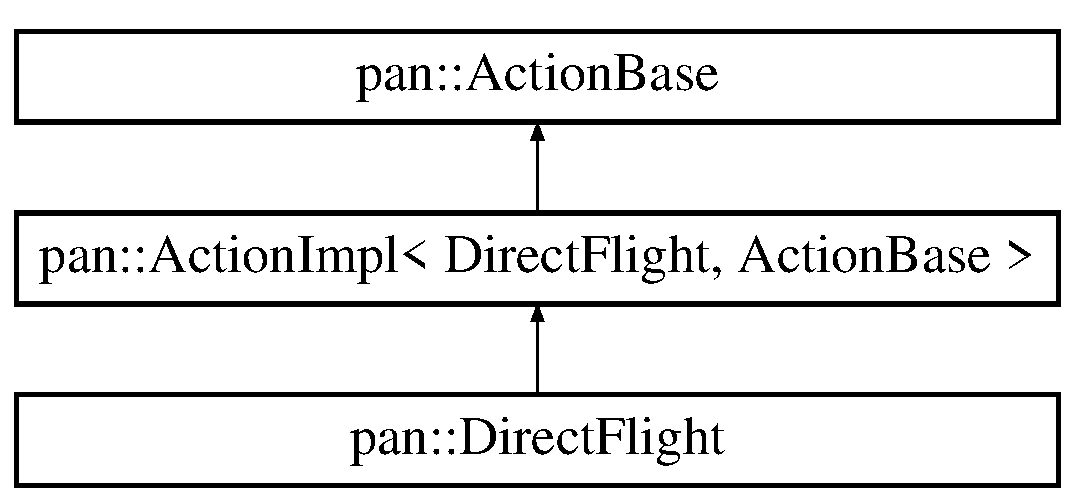
\includegraphics[height=3.000000cm]{classpan_1_1_direct_flight}
\end{center}
\end{figure}
\subsection*{Public Member Functions}
\begin{DoxyCompactItemize}
\item 
\hyperlink{classpan_1_1_direct_flight_adb9d5acdd3f9fd5288861dd53f06dfe7}{Direct\+Flight} (\hyperlink{namespacepan_a0cdabf874fbf1bb3a1f0152d108c2909}{Player\+Index} \hyperlink{classpan_1_1_direct_flight_afe5a2a1f145f99e778cb3cff80b7d54b}{player}, \hyperlink{namespacepan_afaed28aa6603153dcc062a028602d697}{City\+Index} city)
\end{DoxyCompactItemize}
\subsection*{Public Attributes}
\begin{DoxyCompactItemize}
\item 
\hyperlink{namespacepan_a0cdabf874fbf1bb3a1f0152d108c2909}{Player\+Index} \hyperlink{classpan_1_1_direct_flight_afe5a2a1f145f99e778cb3cff80b7d54b}{player}
\item 
\hyperlink{namespacepan_afaed28aa6603153dcc062a028602d697}{City\+Index} \hyperlink{classpan_1_1_direct_flight_a6781e6dab81c55f2ed96352cad0c793d}{target\+City}
\end{DoxyCompactItemize}


\subsection{Detailed Description}
Class representing a direct flight action. 

\begin{DoxyAuthor}{Author}
Hrachya Hakobyan 
\end{DoxyAuthor}


\subsection{Constructor \& Destructor Documentation}
\mbox{\Hypertarget{classpan_1_1_direct_flight_adb9d5acdd3f9fd5288861dd53f06dfe7}\label{classpan_1_1_direct_flight_adb9d5acdd3f9fd5288861dd53f06dfe7}} 
\index{pan\+::\+Direct\+Flight@{pan\+::\+Direct\+Flight}!Direct\+Flight@{Direct\+Flight}}
\index{Direct\+Flight@{Direct\+Flight}!pan\+::\+Direct\+Flight@{pan\+::\+Direct\+Flight}}
\subsubsection{\texorpdfstring{Direct\+Flight()}{DirectFlight()}}
{\footnotesize\ttfamily pan\+::\+Direct\+Flight\+::\+Direct\+Flight (\begin{DoxyParamCaption}\item[{\hyperlink{namespacepan_a0cdabf874fbf1bb3a1f0152d108c2909}{Player\+Index}}]{player,  }\item[{\hyperlink{namespacepan_afaed28aa6603153dcc062a028602d697}{City\+Index}}]{city }\end{DoxyParamCaption})}



\subsection{Member Data Documentation}
\mbox{\Hypertarget{classpan_1_1_direct_flight_afe5a2a1f145f99e778cb3cff80b7d54b}\label{classpan_1_1_direct_flight_afe5a2a1f145f99e778cb3cff80b7d54b}} 
\index{pan\+::\+Direct\+Flight@{pan\+::\+Direct\+Flight}!player@{player}}
\index{player@{player}!pan\+::\+Direct\+Flight@{pan\+::\+Direct\+Flight}}
\subsubsection{\texorpdfstring{player}{player}}
{\footnotesize\ttfamily \hyperlink{namespacepan_a0cdabf874fbf1bb3a1f0152d108c2909}{Player\+Index} pan\+::\+Direct\+Flight\+::player}

\mbox{\Hypertarget{classpan_1_1_direct_flight_a6781e6dab81c55f2ed96352cad0c793d}\label{classpan_1_1_direct_flight_a6781e6dab81c55f2ed96352cad0c793d}} 
\index{pan\+::\+Direct\+Flight@{pan\+::\+Direct\+Flight}!target\+City@{target\+City}}
\index{target\+City@{target\+City}!pan\+::\+Direct\+Flight@{pan\+::\+Direct\+Flight}}
\subsubsection{\texorpdfstring{target\+City}{targetCity}}
{\footnotesize\ttfamily \hyperlink{namespacepan_afaed28aa6603153dcc062a028602d697}{City\+Index} pan\+::\+Direct\+Flight\+::target\+City}



The documentation for this class was generated from the following files\+:\begin{DoxyCompactItemize}
\item 
\hyperlink{_direct_flight_8h}{Direct\+Flight.\+h}\item 
\hyperlink{_direct_flight_8cpp}{Direct\+Flight.\+cpp}\end{DoxyCompactItemize}

\hypertarget{classpan_1_1_discard_card}{}\section{pan\+:\+:Discard\+Card Class Reference}
\label{classpan_1_1_discard_card}\index{pan\+::\+Discard\+Card@{pan\+::\+Discard\+Card}}


Class representing the action of a player discarding a card.  




{\ttfamily \#include $<$Discard\+Card.\+h$>$}

Inheritance diagram for pan\+:\+:Discard\+Card\+:\begin{figure}[H]
\begin{center}
\leavevmode
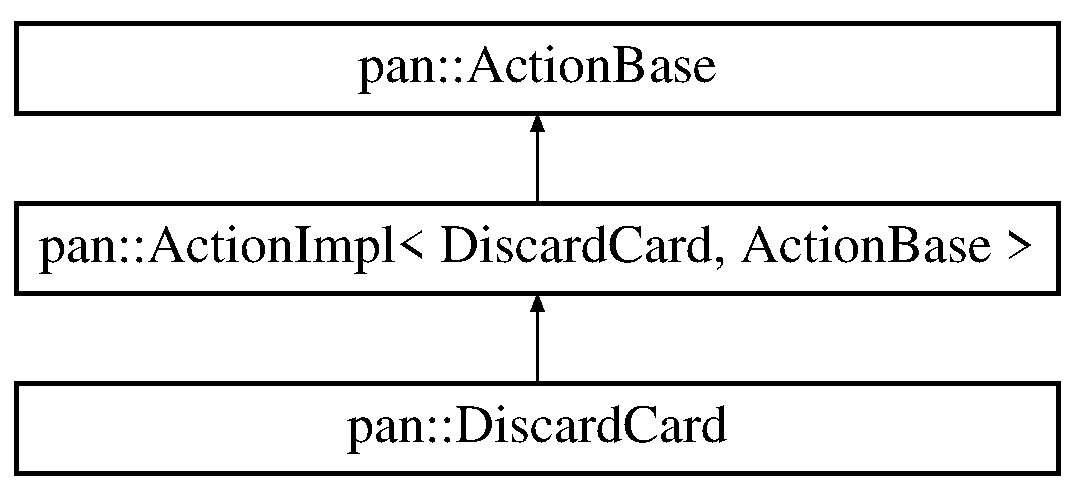
\includegraphics[height=3.000000cm]{classpan_1_1_discard_card}
\end{center}
\end{figure}
\subsection*{Public Member Functions}
\begin{DoxyCompactItemize}
\item 
\hyperlink{classpan_1_1_discard_card_a5a4f4d975057d33f91e857a1b36b275b}{Discard\+Card} (\hyperlink{namespacepan_a0cdabf874fbf1bb3a1f0152d108c2909}{Player\+Index} \hyperlink{classpan_1_1_discard_card_a92d202c3983f09cac6ad0350b10359a9}{player}, unsigned int \hyperlink{classpan_1_1_discard_card_a62efd70c54ac4e21ec4d5c719bd8ef23}{index})
\end{DoxyCompactItemize}
\subsection*{Public Attributes}
\begin{DoxyCompactItemize}
\item 
\hyperlink{namespacepan_a0cdabf874fbf1bb3a1f0152d108c2909}{Player\+Index} \hyperlink{classpan_1_1_discard_card_a92d202c3983f09cac6ad0350b10359a9}{player}
\item 
unsigned int \hyperlink{classpan_1_1_discard_card_a62efd70c54ac4e21ec4d5c719bd8ef23}{index}
\end{DoxyCompactItemize}


\subsection{Detailed Description}
Class representing the action of a player discarding a card. 

\begin{DoxyAuthor}{Author}
Hrachya Hakobyan 
\end{DoxyAuthor}


\subsection{Constructor \& Destructor Documentation}
\mbox{\Hypertarget{classpan_1_1_discard_card_a5a4f4d975057d33f91e857a1b36b275b}\label{classpan_1_1_discard_card_a5a4f4d975057d33f91e857a1b36b275b}} 
\index{pan\+::\+Discard\+Card@{pan\+::\+Discard\+Card}!Discard\+Card@{Discard\+Card}}
\index{Discard\+Card@{Discard\+Card}!pan\+::\+Discard\+Card@{pan\+::\+Discard\+Card}}
\subsubsection{\texorpdfstring{Discard\+Card()}{DiscardCard()}}
{\footnotesize\ttfamily pan\+::\+Discard\+Card\+::\+Discard\+Card (\begin{DoxyParamCaption}\item[{\hyperlink{namespacepan_a0cdabf874fbf1bb3a1f0152d108c2909}{Player\+Index}}]{player,  }\item[{unsigned int}]{index }\end{DoxyParamCaption})}



\subsection{Member Data Documentation}
\mbox{\Hypertarget{classpan_1_1_discard_card_a62efd70c54ac4e21ec4d5c719bd8ef23}\label{classpan_1_1_discard_card_a62efd70c54ac4e21ec4d5c719bd8ef23}} 
\index{pan\+::\+Discard\+Card@{pan\+::\+Discard\+Card}!index@{index}}
\index{index@{index}!pan\+::\+Discard\+Card@{pan\+::\+Discard\+Card}}
\subsubsection{\texorpdfstring{index}{index}}
{\footnotesize\ttfamily unsigned int pan\+::\+Discard\+Card\+::index}

\mbox{\Hypertarget{classpan_1_1_discard_card_a92d202c3983f09cac6ad0350b10359a9}\label{classpan_1_1_discard_card_a92d202c3983f09cac6ad0350b10359a9}} 
\index{pan\+::\+Discard\+Card@{pan\+::\+Discard\+Card}!player@{player}}
\index{player@{player}!pan\+::\+Discard\+Card@{pan\+::\+Discard\+Card}}
\subsubsection{\texorpdfstring{player}{player}}
{\footnotesize\ttfamily \hyperlink{namespacepan_a0cdabf874fbf1bb3a1f0152d108c2909}{Player\+Index} pan\+::\+Discard\+Card\+::player}



The documentation for this class was generated from the following files\+:\begin{DoxyCompactItemize}
\item 
\hyperlink{_discard_card_8h}{Discard\+Card.\+h}\item 
\hyperlink{_discard_card_8cpp}{Discard\+Card.\+cpp}\end{DoxyCompactItemize}

\hypertarget{classpan_1_1_discover_cure}{}\section{pan\+:\+:Discover\+Cure Class Reference}
\label{classpan_1_1_discover_cure}\index{pan\+::\+Discover\+Cure@{pan\+::\+Discover\+Cure}}


Class representing a discover cure action.  




{\ttfamily \#include $<$Discover\+Cure.\+h$>$}

Inheritance diagram for pan\+:\+:Discover\+Cure\+:\begin{figure}[H]
\begin{center}
\leavevmode
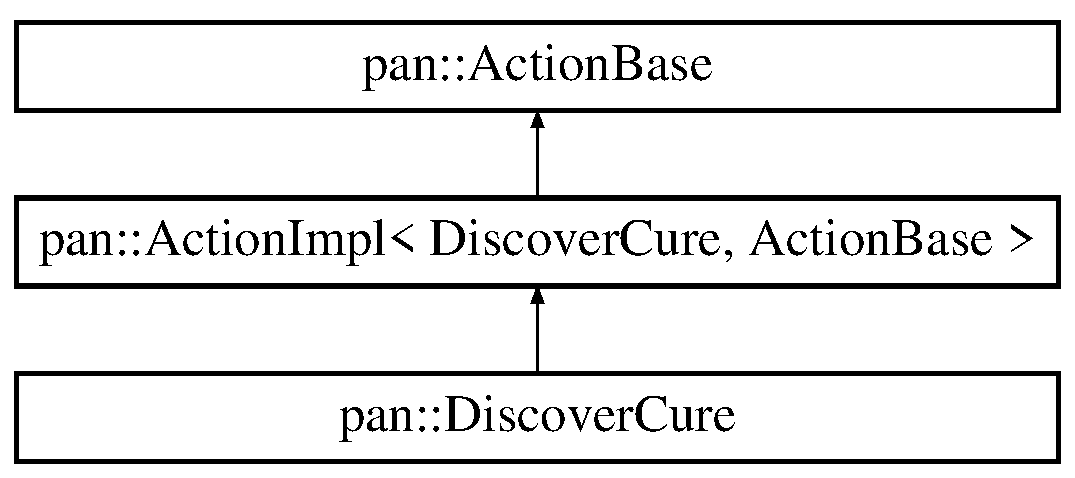
\includegraphics[height=3.000000cm]{classpan_1_1_discover_cure}
\end{center}
\end{figure}
\subsection*{Public Member Functions}
\begin{DoxyCompactItemize}
\item 
\hyperlink{classpan_1_1_discover_cure_a8619beb1af3c6dff42028831762b9dbe}{Discover\+Cure} (\hyperlink{namespacepan_a0cdabf874fbf1bb3a1f0152d108c2909}{Player\+Index} \hyperlink{classpan_1_1_discover_cure_a32a25e9bc1bb54c98d9a96c47c991ed7}{player}, \hyperlink{namespacepan_a48851b51b0aef3f0e1be80df5031d9d7}{Disease\+Type} d\+Type)
\end{DoxyCompactItemize}
\subsection*{Public Attributes}
\begin{DoxyCompactItemize}
\item 
\hyperlink{namespacepan_a0cdabf874fbf1bb3a1f0152d108c2909}{Player\+Index} \hyperlink{classpan_1_1_discover_cure_a32a25e9bc1bb54c98d9a96c47c991ed7}{player}
\item 
\hyperlink{namespacepan_a48851b51b0aef3f0e1be80df5031d9d7}{Disease\+Type} \hyperlink{classpan_1_1_discover_cure_ac5add4642696af23f73e024dfe1ec520}{disease\+Type}
\end{DoxyCompactItemize}


\subsection{Detailed Description}
Class representing a discover cure action. 

\begin{DoxyAuthor}{Author}
Hrachya Hakobyan 
\end{DoxyAuthor}


\subsection{Constructor \& Destructor Documentation}
\mbox{\Hypertarget{classpan_1_1_discover_cure_a8619beb1af3c6dff42028831762b9dbe}\label{classpan_1_1_discover_cure_a8619beb1af3c6dff42028831762b9dbe}} 
\index{pan\+::\+Discover\+Cure@{pan\+::\+Discover\+Cure}!Discover\+Cure@{Discover\+Cure}}
\index{Discover\+Cure@{Discover\+Cure}!pan\+::\+Discover\+Cure@{pan\+::\+Discover\+Cure}}
\subsubsection{\texorpdfstring{Discover\+Cure()}{DiscoverCure()}}
{\footnotesize\ttfamily pan\+::\+Discover\+Cure\+::\+Discover\+Cure (\begin{DoxyParamCaption}\item[{\hyperlink{namespacepan_a0cdabf874fbf1bb3a1f0152d108c2909}{Player\+Index}}]{player,  }\item[{\hyperlink{namespacepan_a48851b51b0aef3f0e1be80df5031d9d7}{Disease\+Type}}]{d\+Type }\end{DoxyParamCaption})}



\subsection{Member Data Documentation}
\mbox{\Hypertarget{classpan_1_1_discover_cure_ac5add4642696af23f73e024dfe1ec520}\label{classpan_1_1_discover_cure_ac5add4642696af23f73e024dfe1ec520}} 
\index{pan\+::\+Discover\+Cure@{pan\+::\+Discover\+Cure}!disease\+Type@{disease\+Type}}
\index{disease\+Type@{disease\+Type}!pan\+::\+Discover\+Cure@{pan\+::\+Discover\+Cure}}
\subsubsection{\texorpdfstring{disease\+Type}{diseaseType}}
{\footnotesize\ttfamily \hyperlink{namespacepan_a48851b51b0aef3f0e1be80df5031d9d7}{Disease\+Type} pan\+::\+Discover\+Cure\+::disease\+Type}

\mbox{\Hypertarget{classpan_1_1_discover_cure_a32a25e9bc1bb54c98d9a96c47c991ed7}\label{classpan_1_1_discover_cure_a32a25e9bc1bb54c98d9a96c47c991ed7}} 
\index{pan\+::\+Discover\+Cure@{pan\+::\+Discover\+Cure}!player@{player}}
\index{player@{player}!pan\+::\+Discover\+Cure@{pan\+::\+Discover\+Cure}}
\subsubsection{\texorpdfstring{player}{player}}
{\footnotesize\ttfamily \hyperlink{namespacepan_a0cdabf874fbf1bb3a1f0152d108c2909}{Player\+Index} pan\+::\+Discover\+Cure\+::player}



The documentation for this class was generated from the following files\+:\begin{DoxyCompactItemize}
\item 
\hyperlink{_discover_cure_8h}{Discover\+Cure.\+h}\item 
\hyperlink{_discover_cure_8cpp}{Discover\+Cure.\+cpp}\end{DoxyCompactItemize}

\hypertarget{classpan_1_1_disease}{}\section{pan\+:\+:Disease Class Reference}
\label{classpan_1_1_disease}\index{pan\+::\+Disease@{pan\+::\+Disease}}


Stores disease state.  




{\ttfamily \#include $<$Disease.\+h$>$}

Inheritance diagram for pan\+:\+:Disease\+:\begin{figure}[H]
\begin{center}
\leavevmode
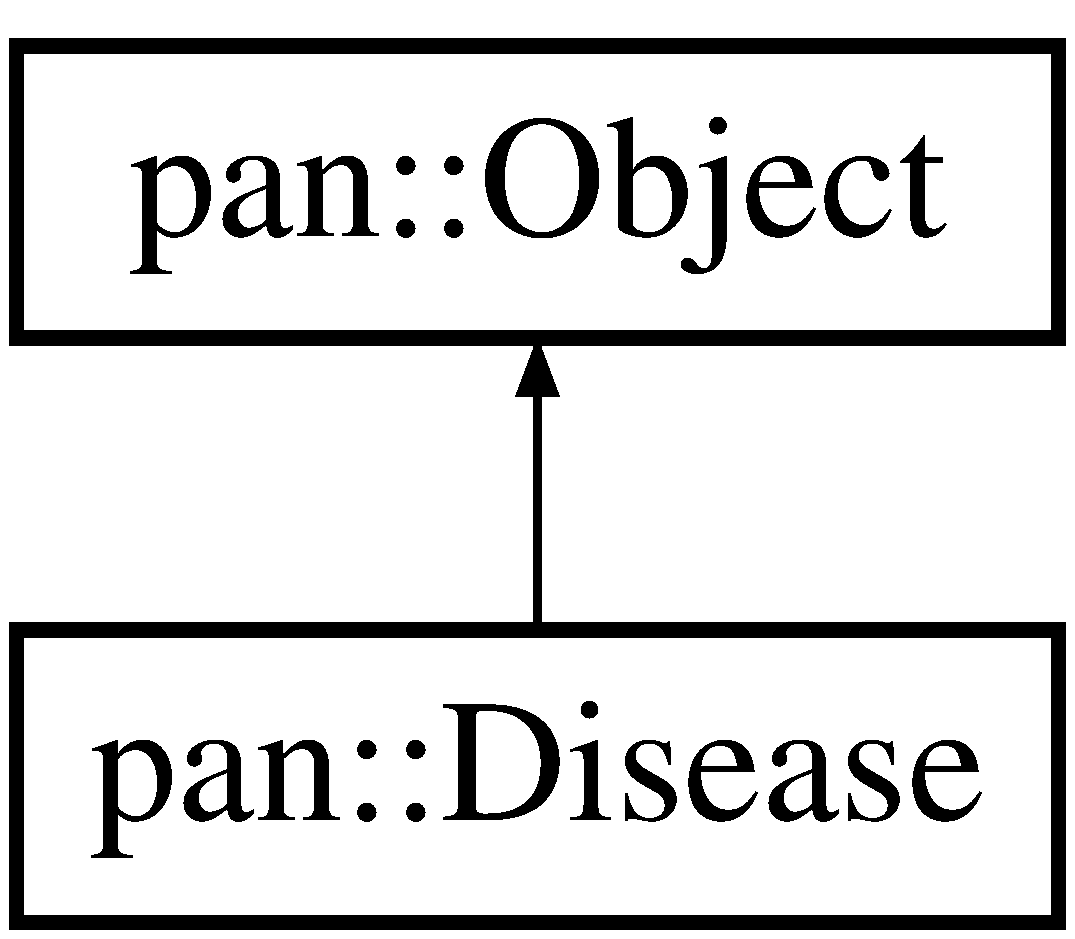
\includegraphics[height=2.000000cm]{classpan_1_1_disease}
\end{center}
\end{figure}
\subsection*{Public Member Functions}
\begin{DoxyCompactItemize}
\item 
\hyperlink{classpan_1_1_disease_a5be3dc7f12596a1bc6221cad3faf5245}{Disease} (\hyperlink{namespacepan_a48851b51b0aef3f0e1be80df5031d9d7}{Disease\+Type} disease\+Type=0)
\item 
\hyperlink{classpan_1_1_disease_a887d5b552c8c868211101b3ba349239b}{Disease} (const \hyperlink{classpan_1_1_disease}{Disease} \&)
\item 
\hyperlink{classpan_1_1_disease}{Disease} \& \hyperlink{classpan_1_1_disease_a7f828d68e1c0cccc7bffcef529ab547f}{operator=} (const \hyperlink{classpan_1_1_disease}{Disease} \&)
\item 
\hyperlink{classpan_1_1_disease_a0bb1181ae59b3d54f6968a1260726102}{$\sim$\+Disease} ()=default
\item 
bool \hyperlink{classpan_1_1_disease_a7a39321c5b39468d2ac0cd8ff2abafc2}{get\+Is\+Cured} () const
\item 
bool \hyperlink{classpan_1_1_disease_afe3ad8194b4bfa1fd25eb833ba8ade10}{get\+Is\+Eradicated} () const
\item 
\hyperlink{namespacepan_a48851b51b0aef3f0e1be80df5031d9d7}{Disease\+Type} \hyperlink{classpan_1_1_disease_adf3b7990f5986899944ec7b82131278d}{get\+Diseae\+Type} () const
\item 
void \hyperlink{classpan_1_1_disease_ac6363817626fee5081df5ff3c4be2b68}{set\+Is\+Cured} (bool is\+Cured)
\item 
void \hyperlink{classpan_1_1_disease_a21c70c565e8a186f699696159231a767}{set\+Is\+Eradicated} (bool is\+Eradicated)
\item 
std\+::string \hyperlink{classpan_1_1_disease_a56ea3e8918baf355ad2d1aa253fd9f65}{description} () const
\item 
bool \hyperlink{classpan_1_1_disease_a8f0c036eba650a230abb91bd8334d150}{operator==} (const \hyperlink{classpan_1_1_disease}{Disease} \&) const
\item 
bool \hyperlink{classpan_1_1_disease_ae699486ffe1bf9e35d1847bc1b8d2617}{operator!=} (const \hyperlink{classpan_1_1_disease}{Disease} \&) const
\item 
{\footnotesize template$<$class Archive $>$ }\\void \hyperlink{classpan_1_1_disease_a6fcfb95df953d991c96188ea2966583a}{serialize} (Archive \&ar, const unsigned int)
\end{DoxyCompactItemize}
\subsection*{Friends}
\begin{DoxyCompactItemize}
\item 
class \hyperlink{classpan_1_1_disease_ac98d07dd8f7b70e16ccb9a01abf56b9c}{boost\+::serialization\+::access}
\end{DoxyCompactItemize}


\subsection{Detailed Description}
Stores disease state. 

\begin{DoxyAuthor}{Author}
Hrachya Hakobyan 
\end{DoxyAuthor}


\subsection{Constructor \& Destructor Documentation}
\mbox{\Hypertarget{classpan_1_1_disease_a5be3dc7f12596a1bc6221cad3faf5245}\label{classpan_1_1_disease_a5be3dc7f12596a1bc6221cad3faf5245}} 
\index{pan\+::\+Disease@{pan\+::\+Disease}!Disease@{Disease}}
\index{Disease@{Disease}!pan\+::\+Disease@{pan\+::\+Disease}}
\subsubsection{\texorpdfstring{Disease()}{Disease()}\hspace{0.1cm}{\footnotesize\ttfamily [1/2]}}
{\footnotesize\ttfamily pan\+::\+Disease\+::\+Disease (\begin{DoxyParamCaption}\item[{\hyperlink{namespacepan_a48851b51b0aef3f0e1be80df5031d9d7}{Disease\+Type}}]{disease\+Type = {\ttfamily 0} }\end{DoxyParamCaption})}

\mbox{\Hypertarget{classpan_1_1_disease_a887d5b552c8c868211101b3ba349239b}\label{classpan_1_1_disease_a887d5b552c8c868211101b3ba349239b}} 
\index{pan\+::\+Disease@{pan\+::\+Disease}!Disease@{Disease}}
\index{Disease@{Disease}!pan\+::\+Disease@{pan\+::\+Disease}}
\subsubsection{\texorpdfstring{Disease()}{Disease()}\hspace{0.1cm}{\footnotesize\ttfamily [2/2]}}
{\footnotesize\ttfamily pan\+::\+Disease\+::\+Disease (\begin{DoxyParamCaption}\item[{const \hyperlink{classpan_1_1_disease}{Disease} \&}]{o }\end{DoxyParamCaption})}

\mbox{\Hypertarget{classpan_1_1_disease_a0bb1181ae59b3d54f6968a1260726102}\label{classpan_1_1_disease_a0bb1181ae59b3d54f6968a1260726102}} 
\index{pan\+::\+Disease@{pan\+::\+Disease}!````~Disease@{$\sim$\+Disease}}
\index{````~Disease@{$\sim$\+Disease}!pan\+::\+Disease@{pan\+::\+Disease}}
\subsubsection{\texorpdfstring{$\sim$\+Disease()}{~Disease()}}
{\footnotesize\ttfamily pan\+::\+Disease\+::$\sim$\+Disease (\begin{DoxyParamCaption}{ }\end{DoxyParamCaption})\hspace{0.3cm}{\ttfamily [default]}}



\subsection{Member Function Documentation}
\mbox{\Hypertarget{classpan_1_1_disease_a56ea3e8918baf355ad2d1aa253fd9f65}\label{classpan_1_1_disease_a56ea3e8918baf355ad2d1aa253fd9f65}} 
\index{pan\+::\+Disease@{pan\+::\+Disease}!description@{description}}
\index{description@{description}!pan\+::\+Disease@{pan\+::\+Disease}}
\subsubsection{\texorpdfstring{description()}{description()}}
{\footnotesize\ttfamily std\+::string pan\+::\+Disease\+::description (\begin{DoxyParamCaption}{ }\end{DoxyParamCaption}) const\hspace{0.3cm}{\ttfamily [inline]}, {\ttfamily [virtual]}}



Implements \hyperlink{classpan_1_1_object_a2bb6d3117bb32f5774657c83f118ed8b}{pan\+::\+Object}.

\mbox{\Hypertarget{classpan_1_1_disease_adf3b7990f5986899944ec7b82131278d}\label{classpan_1_1_disease_adf3b7990f5986899944ec7b82131278d}} 
\index{pan\+::\+Disease@{pan\+::\+Disease}!get\+Diseae\+Type@{get\+Diseae\+Type}}
\index{get\+Diseae\+Type@{get\+Diseae\+Type}!pan\+::\+Disease@{pan\+::\+Disease}}
\subsubsection{\texorpdfstring{get\+Diseae\+Type()}{getDiseaeType()}}
{\footnotesize\ttfamily \hyperlink{namespacepan_a48851b51b0aef3f0e1be80df5031d9d7}{Disease\+Type} pan\+::\+Disease\+::get\+Diseae\+Type (\begin{DoxyParamCaption}{ }\end{DoxyParamCaption}) const\hspace{0.3cm}{\ttfamily [inline]}}

\mbox{\Hypertarget{classpan_1_1_disease_a7a39321c5b39468d2ac0cd8ff2abafc2}\label{classpan_1_1_disease_a7a39321c5b39468d2ac0cd8ff2abafc2}} 
\index{pan\+::\+Disease@{pan\+::\+Disease}!get\+Is\+Cured@{get\+Is\+Cured}}
\index{get\+Is\+Cured@{get\+Is\+Cured}!pan\+::\+Disease@{pan\+::\+Disease}}
\subsubsection{\texorpdfstring{get\+Is\+Cured()}{getIsCured()}}
{\footnotesize\ttfamily bool pan\+::\+Disease\+::get\+Is\+Cured (\begin{DoxyParamCaption}{ }\end{DoxyParamCaption}) const\hspace{0.3cm}{\ttfamily [inline]}}

\mbox{\Hypertarget{classpan_1_1_disease_afe3ad8194b4bfa1fd25eb833ba8ade10}\label{classpan_1_1_disease_afe3ad8194b4bfa1fd25eb833ba8ade10}} 
\index{pan\+::\+Disease@{pan\+::\+Disease}!get\+Is\+Eradicated@{get\+Is\+Eradicated}}
\index{get\+Is\+Eradicated@{get\+Is\+Eradicated}!pan\+::\+Disease@{pan\+::\+Disease}}
\subsubsection{\texorpdfstring{get\+Is\+Eradicated()}{getIsEradicated()}}
{\footnotesize\ttfamily bool pan\+::\+Disease\+::get\+Is\+Eradicated (\begin{DoxyParamCaption}{ }\end{DoxyParamCaption}) const\hspace{0.3cm}{\ttfamily [inline]}}

\mbox{\Hypertarget{classpan_1_1_disease_ae699486ffe1bf9e35d1847bc1b8d2617}\label{classpan_1_1_disease_ae699486ffe1bf9e35d1847bc1b8d2617}} 
\index{pan\+::\+Disease@{pan\+::\+Disease}!operator"!=@{operator"!=}}
\index{operator"!=@{operator"!=}!pan\+::\+Disease@{pan\+::\+Disease}}
\subsubsection{\texorpdfstring{operator"!=()}{operator!=()}}
{\footnotesize\ttfamily bool pan\+::\+Disease\+::operator!= (\begin{DoxyParamCaption}\item[{const \hyperlink{classpan_1_1_disease}{Disease} \&}]{o }\end{DoxyParamCaption}) const\hspace{0.3cm}{\ttfamily [inline]}}

\mbox{\Hypertarget{classpan_1_1_disease_a7f828d68e1c0cccc7bffcef529ab547f}\label{classpan_1_1_disease_a7f828d68e1c0cccc7bffcef529ab547f}} 
\index{pan\+::\+Disease@{pan\+::\+Disease}!operator=@{operator=}}
\index{operator=@{operator=}!pan\+::\+Disease@{pan\+::\+Disease}}
\subsubsection{\texorpdfstring{operator=()}{operator=()}}
{\footnotesize\ttfamily \hyperlink{classpan_1_1_disease}{Disease} \& pan\+::\+Disease\+::operator= (\begin{DoxyParamCaption}\item[{const \hyperlink{classpan_1_1_disease}{Disease} \&}]{o }\end{DoxyParamCaption})}

\mbox{\Hypertarget{classpan_1_1_disease_a8f0c036eba650a230abb91bd8334d150}\label{classpan_1_1_disease_a8f0c036eba650a230abb91bd8334d150}} 
\index{pan\+::\+Disease@{pan\+::\+Disease}!operator==@{operator==}}
\index{operator==@{operator==}!pan\+::\+Disease@{pan\+::\+Disease}}
\subsubsection{\texorpdfstring{operator==()}{operator==()}}
{\footnotesize\ttfamily bool pan\+::\+Disease\+::operator== (\begin{DoxyParamCaption}\item[{const \hyperlink{classpan_1_1_disease}{Disease} \&}]{o }\end{DoxyParamCaption}) const\hspace{0.3cm}{\ttfamily [inline]}}

\mbox{\Hypertarget{classpan_1_1_disease_a6fcfb95df953d991c96188ea2966583a}\label{classpan_1_1_disease_a6fcfb95df953d991c96188ea2966583a}} 
\index{pan\+::\+Disease@{pan\+::\+Disease}!serialize@{serialize}}
\index{serialize@{serialize}!pan\+::\+Disease@{pan\+::\+Disease}}
\subsubsection{\texorpdfstring{serialize()}{serialize()}}
{\footnotesize\ttfamily template$<$class Archive $>$ \\
void pan\+::\+Disease\+::serialize (\begin{DoxyParamCaption}\item[{Archive \&}]{ar,  }\item[{const unsigned}]{int }\end{DoxyParamCaption})\hspace{0.3cm}{\ttfamily [inline]}}

\mbox{\Hypertarget{classpan_1_1_disease_ac6363817626fee5081df5ff3c4be2b68}\label{classpan_1_1_disease_ac6363817626fee5081df5ff3c4be2b68}} 
\index{pan\+::\+Disease@{pan\+::\+Disease}!set\+Is\+Cured@{set\+Is\+Cured}}
\index{set\+Is\+Cured@{set\+Is\+Cured}!pan\+::\+Disease@{pan\+::\+Disease}}
\subsubsection{\texorpdfstring{set\+Is\+Cured()}{setIsCured()}}
{\footnotesize\ttfamily void pan\+::\+Disease\+::set\+Is\+Cured (\begin{DoxyParamCaption}\item[{bool}]{is\+Cured }\end{DoxyParamCaption})}

\mbox{\Hypertarget{classpan_1_1_disease_a21c70c565e8a186f699696159231a767}\label{classpan_1_1_disease_a21c70c565e8a186f699696159231a767}} 
\index{pan\+::\+Disease@{pan\+::\+Disease}!set\+Is\+Eradicated@{set\+Is\+Eradicated}}
\index{set\+Is\+Eradicated@{set\+Is\+Eradicated}!pan\+::\+Disease@{pan\+::\+Disease}}
\subsubsection{\texorpdfstring{set\+Is\+Eradicated()}{setIsEradicated()}}
{\footnotesize\ttfamily void pan\+::\+Disease\+::set\+Is\+Eradicated (\begin{DoxyParamCaption}\item[{bool}]{is\+Eradicated }\end{DoxyParamCaption})}



\subsection{Friends And Related Function Documentation}
\mbox{\Hypertarget{classpan_1_1_disease_ac98d07dd8f7b70e16ccb9a01abf56b9c}\label{classpan_1_1_disease_ac98d07dd8f7b70e16ccb9a01abf56b9c}} 
\index{pan\+::\+Disease@{pan\+::\+Disease}!boost\+::serialization\+::access@{boost\+::serialization\+::access}}
\index{boost\+::serialization\+::access@{boost\+::serialization\+::access}!pan\+::\+Disease@{pan\+::\+Disease}}
\subsubsection{\texorpdfstring{boost\+::serialization\+::access}{boost::serialization::access}}
{\footnotesize\ttfamily friend class boost\+::serialization\+::access\hspace{0.3cm}{\ttfamily [friend]}}



The documentation for this class was generated from the following files\+:\begin{DoxyCompactItemize}
\item 
\hyperlink{_disease_8h}{Disease.\+h}\item 
\hyperlink{_disease_8cpp}{Disease.\+cpp}\end{DoxyCompactItemize}

\hypertarget{classpan_1_1_draw_player_cards}{}\section{pan\+:\+:Draw\+Player\+Cards Class Reference}
\label{classpan_1_1_draw_player_cards}\index{pan\+::\+Draw\+Player\+Cards@{pan\+::\+Draw\+Player\+Cards}}


Class representing the action of a player drawing player cards.  




{\ttfamily \#include $<$Draw\+Player\+Cards.\+h$>$}

Inheritance diagram for pan\+:\+:Draw\+Player\+Cards\+:\begin{figure}[H]
\begin{center}
\leavevmode
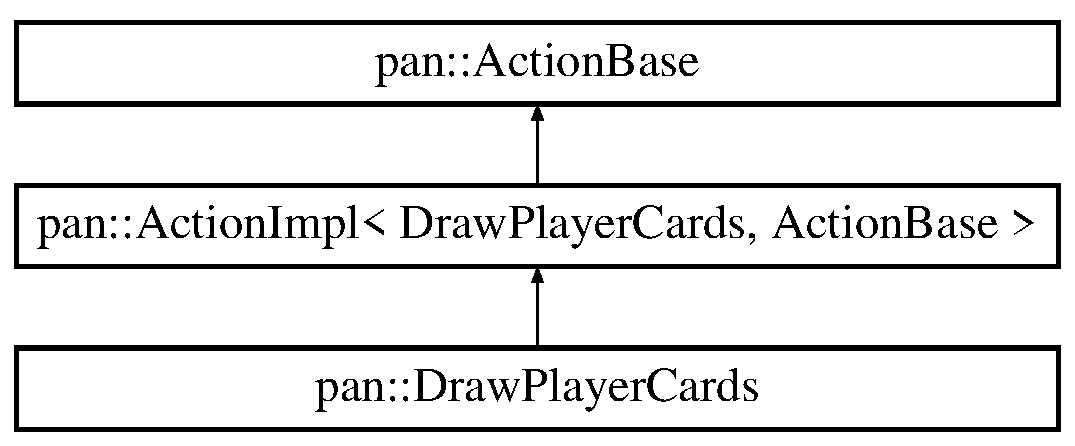
\includegraphics[height=3.000000cm]{classpan_1_1_draw_player_cards}
\end{center}
\end{figure}
\subsection*{Public Member Functions}
\begin{DoxyCompactItemize}
\item 
\hyperlink{classpan_1_1_draw_player_cards_ad76432d661eb15b69cc3236fd8f4f896}{Draw\+Player\+Cards} (\hyperlink{namespacepan_a0cdabf874fbf1bb3a1f0152d108c2909}{Player\+Index} \hyperlink{classpan_1_1_draw_player_cards_a62969ce5dc8a1eeaa104acd073d3971b}{player})
\end{DoxyCompactItemize}
\subsection*{Public Attributes}
\begin{DoxyCompactItemize}
\item 
\hyperlink{namespacepan_a0cdabf874fbf1bb3a1f0152d108c2909}{Player\+Index} \hyperlink{classpan_1_1_draw_player_cards_a62969ce5dc8a1eeaa104acd073d3971b}{player}
\end{DoxyCompactItemize}


\subsection{Detailed Description}
Class representing the action of a player drawing player cards. 

\begin{DoxyAuthor}{Author}
Hrachya Hakobyan 
\end{DoxyAuthor}


\subsection{Constructor \& Destructor Documentation}
\mbox{\Hypertarget{classpan_1_1_draw_player_cards_ad76432d661eb15b69cc3236fd8f4f896}\label{classpan_1_1_draw_player_cards_ad76432d661eb15b69cc3236fd8f4f896}} 
\index{pan\+::\+Draw\+Player\+Cards@{pan\+::\+Draw\+Player\+Cards}!Draw\+Player\+Cards@{Draw\+Player\+Cards}}
\index{Draw\+Player\+Cards@{Draw\+Player\+Cards}!pan\+::\+Draw\+Player\+Cards@{pan\+::\+Draw\+Player\+Cards}}
\subsubsection{\texorpdfstring{Draw\+Player\+Cards()}{DrawPlayerCards()}}
{\footnotesize\ttfamily pan\+::\+Draw\+Player\+Cards\+::\+Draw\+Player\+Cards (\begin{DoxyParamCaption}\item[{\hyperlink{namespacepan_a0cdabf874fbf1bb3a1f0152d108c2909}{Player\+Index}}]{player }\end{DoxyParamCaption})}



\subsection{Member Data Documentation}
\mbox{\Hypertarget{classpan_1_1_draw_player_cards_a62969ce5dc8a1eeaa104acd073d3971b}\label{classpan_1_1_draw_player_cards_a62969ce5dc8a1eeaa104acd073d3971b}} 
\index{pan\+::\+Draw\+Player\+Cards@{pan\+::\+Draw\+Player\+Cards}!player@{player}}
\index{player@{player}!pan\+::\+Draw\+Player\+Cards@{pan\+::\+Draw\+Player\+Cards}}
\subsubsection{\texorpdfstring{player}{player}}
{\footnotesize\ttfamily \hyperlink{namespacepan_a0cdabf874fbf1bb3a1f0152d108c2909}{Player\+Index} pan\+::\+Draw\+Player\+Cards\+::player}



The documentation for this class was generated from the following files\+:\begin{DoxyCompactItemize}
\item 
\hyperlink{_draw_player_cards_8h}{Draw\+Player\+Cards.\+h}\item 
\hyperlink{_draw_player_cards_8cpp}{Draw\+Player\+Cards.\+cpp}\end{DoxyCompactItemize}

\hypertarget{classpan_1_1_epidemic}{}\section{pan\+:\+:Epidemic Class Reference}
\label{classpan_1_1_epidemic}\index{pan\+::\+Epidemic@{pan\+::\+Epidemic}}


Entity of epidemic action.  




{\ttfamily \#include $<$Epidemic.\+h$>$}

Inheritance diagram for pan\+:\+:Epidemic\+:\begin{figure}[H]
\begin{center}
\leavevmode
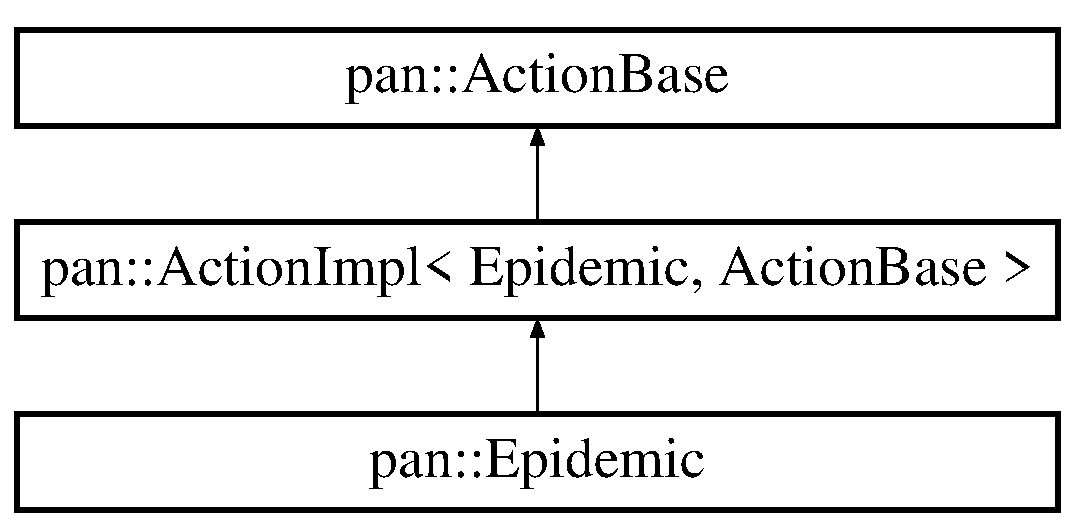
\includegraphics[height=3.000000cm]{classpan_1_1_epidemic}
\end{center}
\end{figure}
\subsection*{Additional Inherited Members}


\subsection{Detailed Description}
Entity of epidemic action. 

\begin{DoxyAuthor}{Author}
Hrachya Hakobyan 
\end{DoxyAuthor}


The documentation for this class was generated from the following file\+:\begin{DoxyCompactItemize}
\item 
\hyperlink{_epidemic_8h}{Epidemic.\+h}\end{DoxyCompactItemize}

\hypertarget{classpan_1_1detail_1_1_factory}{}\section{pan\+:\+:detail\+:\+:Factory$<$ K, T, Us $>$ Class Template Reference}
\label{classpan_1_1detail_1_1_factory}\index{pan\+::detail\+::\+Factory$<$ K, T, Us $>$@{pan\+::detail\+::\+Factory$<$ K, T, Us $>$}}


a modified templated factory with variadic constructor arguments  




{\ttfamily \#include $<$Factory.\+h$>$}

\subsection*{Public Member Functions}
\begin{DoxyCompactItemize}
\item 
\hyperlink{classpan_1_1detail_1_1_factory_a8bede97b9ebe191c4f44d3f466f479b3}{Factory} (const \hyperlink{classpan_1_1detail_1_1_factory}{Factory} \&)=delete
\item 
void \hyperlink{classpan_1_1detail_1_1_factory_a4ef5146a216ceade5b8c0b06bab2a38c}{operator=} (const \hyperlink{classpan_1_1detail_1_1_factory}{Factory} \&)=delete
\item 
{\footnotesize template$<$typename S $>$ }\\void \hyperlink{classpan_1_1detail_1_1_factory_a1618a041575a6f490a327c5ee5b0cefc}{register\+Class} (K id)
\item 
bool \hyperlink{classpan_1_1detail_1_1_factory_ad7abea702880d5355cf37dfe5aba786d}{has\+Class} (K id)
\item 
T $\ast$ \hyperlink{classpan_1_1detail_1_1_factory_a30fe3b9f6541e9f611edb51bd54584e5}{create\+Object} (K id, Us... args)
\end{DoxyCompactItemize}
\subsection*{Static Public Member Functions}
\begin{DoxyCompactItemize}
\item 
static \hyperlink{classpan_1_1detail_1_1_factory}{Factory} \& \hyperlink{classpan_1_1detail_1_1_factory_a8c96fc8688874e5e8dd4532368a562ea}{get\+Instance} ()
\end{DoxyCompactItemize}


\subsection{Detailed Description}
\subsubsection*{template$<$typename K, typename T, typename ... Us$>$\newline
class pan\+::detail\+::\+Factory$<$ K, T, Us $>$}

a modified templated factory with variadic constructor arguments 

\begin{DoxyAuthor}{Author}
Hrachya Hakobyan 
\end{DoxyAuthor}


\subsection{Constructor \& Destructor Documentation}
\mbox{\Hypertarget{classpan_1_1detail_1_1_factory_a8bede97b9ebe191c4f44d3f466f479b3}\label{classpan_1_1detail_1_1_factory_a8bede97b9ebe191c4f44d3f466f479b3}} 
\index{pan\+::detail\+::\+Factory@{pan\+::detail\+::\+Factory}!Factory@{Factory}}
\index{Factory@{Factory}!pan\+::detail\+::\+Factory@{pan\+::detail\+::\+Factory}}
\subsubsection{\texorpdfstring{Factory()}{Factory()}}
{\footnotesize\ttfamily template$<$typename K , typename T , typename ... Us$>$ \\
\hyperlink{classpan_1_1detail_1_1_factory}{pan\+::detail\+::\+Factory}$<$ K, T, Us $>$\+::\hyperlink{classpan_1_1detail_1_1_factory}{Factory} (\begin{DoxyParamCaption}\item[{const \hyperlink{classpan_1_1detail_1_1_factory}{Factory}$<$ K, T, Us $>$ \&}]{ }\end{DoxyParamCaption})\hspace{0.3cm}{\ttfamily [delete]}}



\subsection{Member Function Documentation}
\mbox{\Hypertarget{classpan_1_1detail_1_1_factory_a30fe3b9f6541e9f611edb51bd54584e5}\label{classpan_1_1detail_1_1_factory_a30fe3b9f6541e9f611edb51bd54584e5}} 
\index{pan\+::detail\+::\+Factory@{pan\+::detail\+::\+Factory}!create\+Object@{create\+Object}}
\index{create\+Object@{create\+Object}!pan\+::detail\+::\+Factory@{pan\+::detail\+::\+Factory}}
\subsubsection{\texorpdfstring{create\+Object()}{createObject()}}
{\footnotesize\ttfamily template$<$typename K , typename T , typename ... Us$>$ \\
T$\ast$ \hyperlink{classpan_1_1detail_1_1_factory}{pan\+::detail\+::\+Factory}$<$ K, T, Us $>$\+::create\+Object (\begin{DoxyParamCaption}\item[{K}]{id,  }\item[{Us...}]{args }\end{DoxyParamCaption})\hspace{0.3cm}{\ttfamily [inline]}}

Creates an object based on an id. It will return null if the key doesn\textquotesingle{}t exist


\begin{DoxyParams}{Parameters}
{\em id} & the id of the object to create \\
\hline
\end{DoxyParams}
\begin{DoxyReturn}{Returns}
the new object or null if the object id doesn\textquotesingle{}t exist 
\end{DoxyReturn}
\mbox{\Hypertarget{classpan_1_1detail_1_1_factory_a8c96fc8688874e5e8dd4532368a562ea}\label{classpan_1_1detail_1_1_factory_a8c96fc8688874e5e8dd4532368a562ea}} 
\index{pan\+::detail\+::\+Factory@{pan\+::detail\+::\+Factory}!get\+Instance@{get\+Instance}}
\index{get\+Instance@{get\+Instance}!pan\+::detail\+::\+Factory@{pan\+::detail\+::\+Factory}}
\subsubsection{\texorpdfstring{get\+Instance()}{getInstance()}}
{\footnotesize\ttfamily template$<$typename K , typename T , typename ... Us$>$ \\
static \hyperlink{classpan_1_1detail_1_1_factory}{Factory}\& \hyperlink{classpan_1_1detail_1_1_factory}{pan\+::detail\+::\+Factory}$<$ K, T, Us $>$\+::get\+Instance (\begin{DoxyParamCaption}{ }\end{DoxyParamCaption})\hspace{0.3cm}{\ttfamily [inline]}, {\ttfamily [static]}}

\mbox{\Hypertarget{classpan_1_1detail_1_1_factory_ad7abea702880d5355cf37dfe5aba786d}\label{classpan_1_1detail_1_1_factory_ad7abea702880d5355cf37dfe5aba786d}} 
\index{pan\+::detail\+::\+Factory@{pan\+::detail\+::\+Factory}!has\+Class@{has\+Class}}
\index{has\+Class@{has\+Class}!pan\+::detail\+::\+Factory@{pan\+::detail\+::\+Factory}}
\subsubsection{\texorpdfstring{has\+Class()}{hasClass()}}
{\footnotesize\ttfamily template$<$typename K , typename T , typename ... Us$>$ \\
bool \hyperlink{classpan_1_1detail_1_1_factory}{pan\+::detail\+::\+Factory}$<$ K, T, Us $>$\+::has\+Class (\begin{DoxyParamCaption}\item[{K}]{id }\end{DoxyParamCaption})\hspace{0.3cm}{\ttfamily [inline]}}

Returns true if a given key exists 
\begin{DoxyParams}{Parameters}
{\em id} & the id to check exists \\
\hline
\end{DoxyParams}
\begin{DoxyReturn}{Returns}
true if the id exists 
\end{DoxyReturn}
\mbox{\Hypertarget{classpan_1_1detail_1_1_factory_a4ef5146a216ceade5b8c0b06bab2a38c}\label{classpan_1_1detail_1_1_factory_a4ef5146a216ceade5b8c0b06bab2a38c}} 
\index{pan\+::detail\+::\+Factory@{pan\+::detail\+::\+Factory}!operator=@{operator=}}
\index{operator=@{operator=}!pan\+::detail\+::\+Factory@{pan\+::detail\+::\+Factory}}
\subsubsection{\texorpdfstring{operator=()}{operator=()}}
{\footnotesize\ttfamily template$<$typename K , typename T , typename ... Us$>$ \\
void \hyperlink{classpan_1_1detail_1_1_factory}{pan\+::detail\+::\+Factory}$<$ K, T, Us $>$\+::operator= (\begin{DoxyParamCaption}\item[{const \hyperlink{classpan_1_1detail_1_1_factory}{Factory}$<$ K, T, Us $>$ \&}]{ }\end{DoxyParamCaption})\hspace{0.3cm}{\ttfamily [delete]}}

\mbox{\Hypertarget{classpan_1_1detail_1_1_factory_a1618a041575a6f490a327c5ee5b0cefc}\label{classpan_1_1detail_1_1_factory_a1618a041575a6f490a327c5ee5b0cefc}} 
\index{pan\+::detail\+::\+Factory@{pan\+::detail\+::\+Factory}!register\+Class@{register\+Class}}
\index{register\+Class@{register\+Class}!pan\+::detail\+::\+Factory@{pan\+::detail\+::\+Factory}}
\subsubsection{\texorpdfstring{register\+Class()}{registerClass()}}
{\footnotesize\ttfamily template$<$typename K , typename T , typename ... Us$>$ \\
template$<$typename S $>$ \\
void \hyperlink{classpan_1_1detail_1_1_factory}{pan\+::detail\+::\+Factory}$<$ K, T, Us $>$\+::register\+Class (\begin{DoxyParamCaption}\item[{K}]{id }\end{DoxyParamCaption})\hspace{0.3cm}{\ttfamily [inline]}}

Registers a class to that it can be created via \hyperlink{classpan_1_1detail_1_1_factory_a30fe3b9f6541e9f611edb51bd54584e5}{create\+Object()}


\begin{DoxyParams}{Parameters}
{\em S} & the class to register, this must ve a subclass of T \\
\hline
{\em id} & the id to associate with the class. This ID must be unique \\
\hline
\end{DoxyParams}


The documentation for this class was generated from the following file\+:\begin{DoxyCompactItemize}
\item 
detail/\hyperlink{_factory_8h}{Factory.\+h}\end{DoxyCompactItemize}

\hypertarget{classpan_1_1_file_manager}{}\section{pan\+:\+:File\+Manager Class Reference}
\label{classpan_1_1_file_manager}\index{pan\+::\+File\+Manager@{pan\+::\+File\+Manager}}


Abstracts away the save/load of game objects. The details of the save/load, i.\+e. the filesystem, fileformat will vary depending on the platform.  




{\ttfamily \#include $<$File\+Manager.\+h$>$}

\subsection*{Public Member Functions}
\begin{DoxyCompactItemize}
\item 
\hyperlink{classpan_1_1_file_manager_a4637c4b4f9d1c264d5373eafe9f8ef60}{$\sim$\+File\+Manager} ()=default
\item 
{\footnotesize template$<$typename T $>$ }\\bool \hyperlink{classpan_1_1_file_manager_ab897366e9055e7e251a67d82b1cefcaa}{save} (const T \&t, const std\+::string \&filename, const std\+::string \&dir, bool overwrite=false) const
\item 
{\footnotesize template$<$typename T $>$ }\\bool \hyperlink{classpan_1_1_file_manager_ac0112a350779701a11110042bd053458}{load} (T \&t, const std\+::string \&file, const std\+::string \&dir) const
\item 
std\+::vector$<$ std\+::string $>$ \hyperlink{classpan_1_1_file_manager_af9d8a64e6bd6cae23ee56af2f13a8124}{all\+Files} (const std\+::string \&path) const
\end{DoxyCompactItemize}
\subsection*{Static Public Member Functions}
\begin{DoxyCompactItemize}
\item 
static \hyperlink{classpan_1_1_file_manager}{File\+Manager} \& \hyperlink{classpan_1_1_file_manager_a9c6dc615236819bad04dc9db880db6f6}{get\+Instance} ()
\end{DoxyCompactItemize}


\subsection{Detailed Description}
Abstracts away the save/load of game objects. The details of the save/load, i.\+e. the filesystem, fileformat will vary depending on the platform. 

\begin{DoxyAuthor}{Author}
Hrachya Hakobyan 
\end{DoxyAuthor}


\subsection{Constructor \& Destructor Documentation}
\mbox{\Hypertarget{classpan_1_1_file_manager_a4637c4b4f9d1c264d5373eafe9f8ef60}\label{classpan_1_1_file_manager_a4637c4b4f9d1c264d5373eafe9f8ef60}} 
\index{pan\+::\+File\+Manager@{pan\+::\+File\+Manager}!````~File\+Manager@{$\sim$\+File\+Manager}}
\index{````~File\+Manager@{$\sim$\+File\+Manager}!pan\+::\+File\+Manager@{pan\+::\+File\+Manager}}
\subsubsection{\texorpdfstring{$\sim$\+File\+Manager()}{~FileManager()}}
{\footnotesize\ttfamily pan\+::\+File\+Manager\+::$\sim$\+File\+Manager (\begin{DoxyParamCaption}{ }\end{DoxyParamCaption})\hspace{0.3cm}{\ttfamily [default]}}



\subsection{Member Function Documentation}
\mbox{\Hypertarget{classpan_1_1_file_manager_af9d8a64e6bd6cae23ee56af2f13a8124}\label{classpan_1_1_file_manager_af9d8a64e6bd6cae23ee56af2f13a8124}} 
\index{pan\+::\+File\+Manager@{pan\+::\+File\+Manager}!all\+Files@{all\+Files}}
\index{all\+Files@{all\+Files}!pan\+::\+File\+Manager@{pan\+::\+File\+Manager}}
\subsubsection{\texorpdfstring{all\+Files()}{allFiles()}}
{\footnotesize\ttfamily std\+::vector$<$ std\+::string $>$ pan\+::\+File\+Manager\+::all\+Files (\begin{DoxyParamCaption}\item[{const std\+::string \&}]{path }\end{DoxyParamCaption}) const}

Returns a vector of all save files \begin{DoxyReturn}{Returns}
a vector of Save\+File objects 
\end{DoxyReturn}
\mbox{\Hypertarget{classpan_1_1_file_manager_a9c6dc615236819bad04dc9db880db6f6}\label{classpan_1_1_file_manager_a9c6dc615236819bad04dc9db880db6f6}} 
\index{pan\+::\+File\+Manager@{pan\+::\+File\+Manager}!get\+Instance@{get\+Instance}}
\index{get\+Instance@{get\+Instance}!pan\+::\+File\+Manager@{pan\+::\+File\+Manager}}
\subsubsection{\texorpdfstring{get\+Instance()}{getInstance()}}
{\footnotesize\ttfamily static \hyperlink{classpan_1_1_file_manager}{File\+Manager}\& pan\+::\+File\+Manager\+::get\+Instance (\begin{DoxyParamCaption}{ }\end{DoxyParamCaption})\hspace{0.3cm}{\ttfamily [inline]}, {\ttfamily [static]}}

\mbox{\Hypertarget{classpan_1_1_file_manager_ac0112a350779701a11110042bd053458}\label{classpan_1_1_file_manager_ac0112a350779701a11110042bd053458}} 
\index{pan\+::\+File\+Manager@{pan\+::\+File\+Manager}!load@{load}}
\index{load@{load}!pan\+::\+File\+Manager@{pan\+::\+File\+Manager}}
\subsubsection{\texorpdfstring{load()}{load()}}
{\footnotesize\ttfamily template$<$typename T $>$ \\
bool pan\+::\+File\+Manager\+::load (\begin{DoxyParamCaption}\item[{T \&}]{t,  }\item[{const std\+::string \&}]{file,  }\item[{const std\+::string \&}]{dir }\end{DoxyParamCaption}) const}

Loads a saved object. 
\begin{DoxyParams}{Parameters}
{\em filename} & the savefile of the game \\
\hline
{\em t} & a reference to a T object \\
\hline
\end{DoxyParams}
\begin{DoxyReturn}{Returns}
true if the load was successful, false otherwise 
\end{DoxyReturn}
\mbox{\Hypertarget{classpan_1_1_file_manager_ab897366e9055e7e251a67d82b1cefcaa}\label{classpan_1_1_file_manager_ab897366e9055e7e251a67d82b1cefcaa}} 
\index{pan\+::\+File\+Manager@{pan\+::\+File\+Manager}!save@{save}}
\index{save@{save}!pan\+::\+File\+Manager@{pan\+::\+File\+Manager}}
\subsubsection{\texorpdfstring{save()}{save()}}
{\footnotesize\ttfamily template$<$typename T $>$ \\
bool pan\+::\+File\+Manager\+::save (\begin{DoxyParamCaption}\item[{const T \&}]{t,  }\item[{const std\+::string \&}]{filename,  }\item[{const std\+::string \&}]{dir,  }\item[{bool}]{overwrite = {\ttfamily false} }\end{DoxyParamCaption}) const}

Save an object. 
\begin{DoxyParams}{Parameters}
{\em t} & the object to save \\
\hline
{\em filename} & the name of the save file \\
\hline
{\em overwrite} & whether to overwrite an existing game \\
\hline
\end{DoxyParams}
\begin{DoxyReturn}{Returns}
true if save was successful, false otherwise. 
\end{DoxyReturn}


The documentation for this class was generated from the following files\+:\begin{DoxyCompactItemize}
\item 
\hyperlink{_file_manager_8h}{File\+Manager.\+h}\item 
\hyperlink{_file_manager_8cpp}{File\+Manager.\+cpp}\end{DoxyCompactItemize}

\hypertarget{classpan_1_1_game}{}\section{pan\+:\+:Game Class Reference}
\label{classpan_1_1_game}\index{pan\+::\+Game@{pan\+::\+Game}}


\hyperlink{classpan_1_1_game}{Game} entity which is responsible for connecting different pieces of the game logic together.  




{\ttfamily \#include $<$Game.\+h$>$}

Inheritance diagram for pan\+:\+:Game\+:\begin{figure}[H]
\begin{center}
\leavevmode
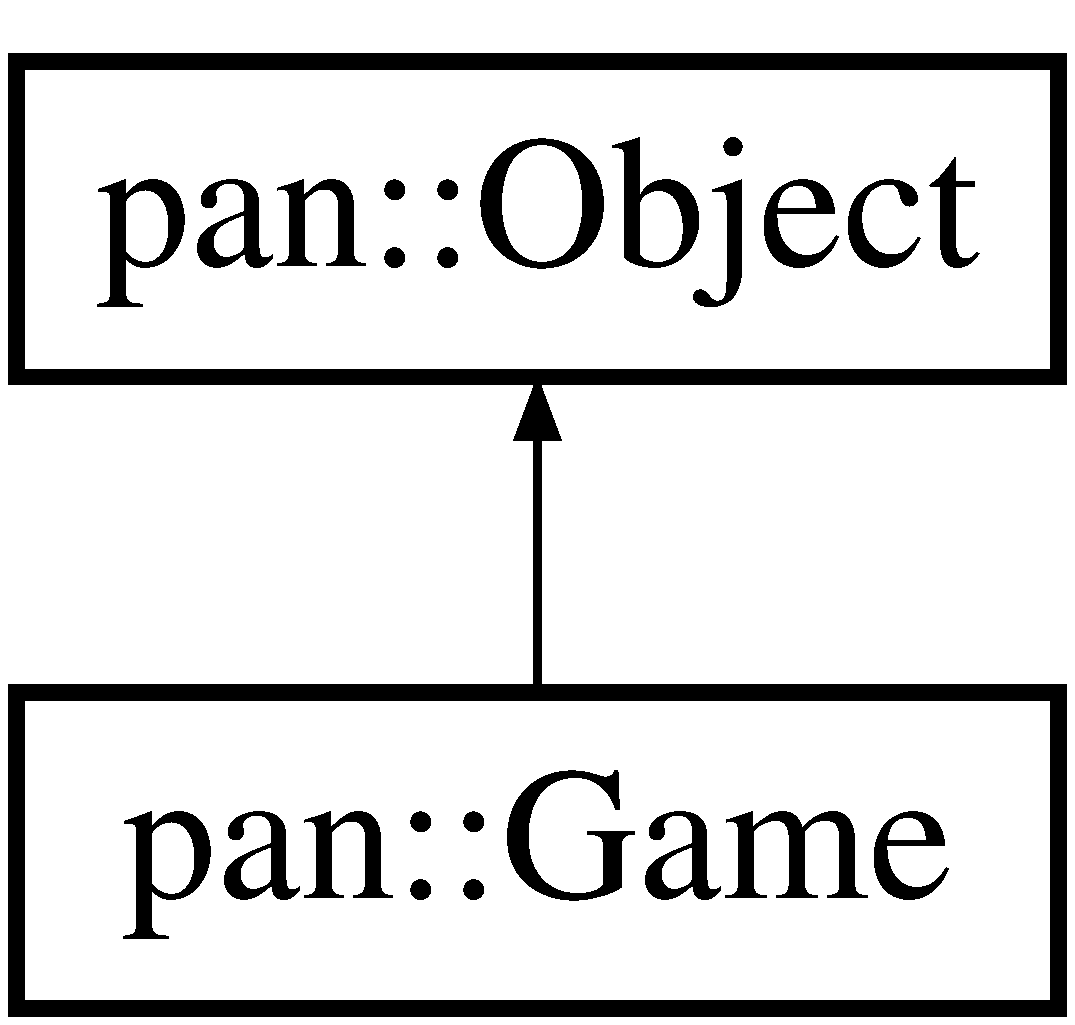
\includegraphics[height=2.000000cm]{classpan_1_1_game}
\end{center}
\end{figure}
\subsection*{Public Member Functions}
\begin{DoxyCompactItemize}
\item 
\hyperlink{classpan_1_1_game_a2c186c7ecac0fded27c7a9db4981a733}{Game} (const \hyperlink{classpan_1_1_settings}{Settings} \&s=\hyperlink{classpan_1_1_settings_a908b6305091cf8d02bb4179dcbbe4ad1}{Settings\+::\+Beginner}(2))
\item 
\hyperlink{classpan_1_1_game_a9dac7dcdc205455639eede641780b701}{Game} (const \hyperlink{classpan_1_1_settings}{Settings} \&s, const \hyperlink{classpan_1_1_map}{Map} \&m)
\item 
\hyperlink{classpan_1_1_game_a95d70ce4840b773525736ee5019433c6}{Game} (const \hyperlink{classpan_1_1_game}{Game} \&)
\item 
\hyperlink{classpan_1_1_game_aedf6e96723a924c772d88f8e7bbee4d8}{Game} (\hyperlink{classpan_1_1_game}{Game} \&\&)
\item 
\hyperlink{classpan_1_1_game}{Game} \& \hyperlink{classpan_1_1_game_a269b24bc583d51e598d22f93232c2f6a}{operator=} (const \hyperlink{classpan_1_1_game}{Game} \&)
\item 
\hyperlink{classpan_1_1_game}{Game} \& \hyperlink{classpan_1_1_game_a6e3665ea2ec133ed5ba0beefadbe688d}{operator=} (\hyperlink{classpan_1_1_game}{Game} \&\&o)
\item 
\hyperlink{classpan_1_1_game_a9ddb30d0a2303334c87048284fa57a63}{$\sim$\+Game} ()
\item 
bool \hyperlink{classpan_1_1_game_a674b783428470d9831cfa79bca8fe0c9}{operator==} (const \hyperlink{classpan_1_1_game}{Game} \&) const
\item 
bool \hyperlink{classpan_1_1_game_a5316baca3fd1487c80759343b0df574a}{operator!=} (const \hyperlink{classpan_1_1_game}{Game} \&) const
\item 
bool \hyperlink{classpan_1_1_game_a164829a91c20f0f1f7b2d32e76e370f2}{initialize} ()
\item 
bool \hyperlink{classpan_1_1_game_a145be880607e15e9ca91ceb36a012de1}{is\+Initialized} () const
\item 
bool \hyperlink{classpan_1_1_game_aa662e441f8910685ef4eb61f76f22354}{is\+Over} () const
\item 
\hyperlink{namespacepan_a6f99370eda3b27c2bbe19b2dacea9212}{Game\+State} \hyperlink{classpan_1_1_game_a1cfa652ea64fb2cb16ded47cec2ea471}{get\+State} () const
\item 
const \hyperlink{classpan_1_1_map}{Map} \& \hyperlink{classpan_1_1_game_a8700fef57be33a7388ef9532dcb30f0c}{get\+Map} () const
\item 
const \hyperlink{structpan_1_1_game_data}{Game\+Data} \& \hyperlink{classpan_1_1_game_a79be06abcb20bc30cc825f8a781d3575}{get\+Game\+Data} () const
\item 
const \hyperlink{structpan_1_1_player_data}{Player\+Data} \& \hyperlink{classpan_1_1_game_a97050486b97c861c3d9d684bc95f0454}{get\+Player\+Data} () const
\item 
const \hyperlink{structpan_1_1_deck_data}{Deck\+Data} \& \hyperlink{classpan_1_1_game_a0fcbd5cc3e1fe836915356478d781fc4}{get\+Deck\+Data} () const
\item 
std\+::string \hyperlink{classpan_1_1_game_a463480ea3f29b34629059134c416ffa0}{description} () const
\item 
std\+::size\+\_\+t \hyperlink{classpan_1_1_game_abd867b6b03f12c8b3aa8ccaef62a9cce}{player\+Count} () const
\item 
const \hyperlink{classpan_1_1_player_base}{Player\+Base} \& \hyperlink{classpan_1_1_game_a23838df4cde7e8be5273ec5de03c152d}{get\+Player} (\hyperlink{namespacepan_a0cdabf874fbf1bb3a1f0152d108c2909}{Player\+Index} i) const
\item 
bool \hyperlink{classpan_1_1_game_aaefd820a874069810f2e62a2d50068e1}{player\+Exists} (\hyperlink{namespacepan_a0cdabf874fbf1bb3a1f0152d108c2909}{Player\+Index} i) const
\item 
void \hyperlink{classpan_1_1_game_a4bcb881db3acea9a02d6ff3ac6e7b209}{add\+Action} (const \hyperlink{classpan_1_1_action_base}{Action\+Base} \&action)
\item 
void \hyperlink{classpan_1_1_game_ad252b2f2c65beb9584ab63d96787fed7}{execute} ()
\item 
void \hyperlink{classpan_1_1_game_a19a92963216ec73c0718cab214f89e85}{execute\+All} ()
\item 
{\footnotesize template$<$Roles R$>$ }\\\hyperlink{namespacepan_a0cdabf874fbf1bb3a1f0152d108c2909}{Player\+Index} \hyperlink{classpan_1_1_game_a0a475cd974dc0de461f7fabc80ab9dce}{add\+Player} (const std\+::string \&name=\char`\"{}\char`\"{})
\item 
\hyperlink{namespacepan_a0cdabf874fbf1bb3a1f0152d108c2909}{Player\+Index} \hyperlink{classpan_1_1_game_adce8b415591cac36cf8f39602f0736c4}{add\+Random\+Player} (const std\+::string \&name=\char`\"{}\char`\"{})
\item 
bool \hyperlink{classpan_1_1_game_a3ed8021afce3a331ede74826bf9742b6}{save} (const std\+::string \&name) const
\end{DoxyCompactItemize}
\subsection*{Static Public Member Functions}
\begin{DoxyCompactItemize}
\item 
static bool \hyperlink{classpan_1_1_game_a3e462af43777e6159bd7ff4c3ca0815c}{load} (const std\+::string \&file, \hyperlink{classpan_1_1_game}{Game} \&game)
\end{DoxyCompactItemize}
\subsection*{Static Public Attributes}
\begin{DoxyCompactItemize}
\item 
static const int \hyperlink{classpan_1_1_game_ade098455080cd39281e873a499331139}{Invalid\+Player\+Index} = -\/1
\end{DoxyCompactItemize}
\subsection*{Friends}
\begin{DoxyCompactItemize}
\item 
class \hyperlink{classpan_1_1_game_a97e74bf016dcec05afd5626a1f2df25a}{Action\+Handler}
\item 
class \hyperlink{classpan_1_1_game_ac98d07dd8f7b70e16ccb9a01abf56b9c}{boost\+::serialization\+::access}
\end{DoxyCompactItemize}


\subsection{Detailed Description}
\hyperlink{classpan_1_1_game}{Game} entity which is responsible for connecting different pieces of the game logic together. 

\begin{DoxyAuthor}{Author}
Hrachya Hakobyan 
\end{DoxyAuthor}


\subsection{Constructor \& Destructor Documentation}
\mbox{\Hypertarget{classpan_1_1_game_a2c186c7ecac0fded27c7a9db4981a733}\label{classpan_1_1_game_a2c186c7ecac0fded27c7a9db4981a733}} 
\index{pan\+::\+Game@{pan\+::\+Game}!Game@{Game}}
\index{Game@{Game}!pan\+::\+Game@{pan\+::\+Game}}
\subsubsection{\texorpdfstring{Game()}{Game()}\hspace{0.1cm}{\footnotesize\ttfamily [1/4]}}
{\footnotesize\ttfamily pan\+::\+Game\+::\+Game (\begin{DoxyParamCaption}\item[{const \hyperlink{classpan_1_1_settings}{Settings} \&}]{s = {\ttfamily \hyperlink{classpan_1_1_settings_a908b6305091cf8d02bb4179dcbbe4ad1}{Settings\+::\+Beginner}(2)} }\end{DoxyParamCaption})}

\mbox{\Hypertarget{classpan_1_1_game_a9dac7dcdc205455639eede641780b701}\label{classpan_1_1_game_a9dac7dcdc205455639eede641780b701}} 
\index{pan\+::\+Game@{pan\+::\+Game}!Game@{Game}}
\index{Game@{Game}!pan\+::\+Game@{pan\+::\+Game}}
\subsubsection{\texorpdfstring{Game()}{Game()}\hspace{0.1cm}{\footnotesize\ttfamily [2/4]}}
{\footnotesize\ttfamily pan\+::\+Game\+::\+Game (\begin{DoxyParamCaption}\item[{const \hyperlink{classpan_1_1_settings}{Settings} \&}]{s,  }\item[{const \hyperlink{classpan_1_1_map}{Map} \&}]{m }\end{DoxyParamCaption})}

\mbox{\Hypertarget{classpan_1_1_game_a95d70ce4840b773525736ee5019433c6}\label{classpan_1_1_game_a95d70ce4840b773525736ee5019433c6}} 
\index{pan\+::\+Game@{pan\+::\+Game}!Game@{Game}}
\index{Game@{Game}!pan\+::\+Game@{pan\+::\+Game}}
\subsubsection{\texorpdfstring{Game()}{Game()}\hspace{0.1cm}{\footnotesize\ttfamily [3/4]}}
{\footnotesize\ttfamily pan\+::\+Game\+::\+Game (\begin{DoxyParamCaption}\item[{const \hyperlink{classpan_1_1_game}{Game} \&}]{o }\end{DoxyParamCaption})}

\mbox{\Hypertarget{classpan_1_1_game_aedf6e96723a924c772d88f8e7bbee4d8}\label{classpan_1_1_game_aedf6e96723a924c772d88f8e7bbee4d8}} 
\index{pan\+::\+Game@{pan\+::\+Game}!Game@{Game}}
\index{Game@{Game}!pan\+::\+Game@{pan\+::\+Game}}
\subsubsection{\texorpdfstring{Game()}{Game()}\hspace{0.1cm}{\footnotesize\ttfamily [4/4]}}
{\footnotesize\ttfamily pan\+::\+Game\+::\+Game (\begin{DoxyParamCaption}\item[{\hyperlink{classpan_1_1_game}{Game} \&\&}]{o }\end{DoxyParamCaption})}

\mbox{\Hypertarget{classpan_1_1_game_a9ddb30d0a2303334c87048284fa57a63}\label{classpan_1_1_game_a9ddb30d0a2303334c87048284fa57a63}} 
\index{pan\+::\+Game@{pan\+::\+Game}!````~Game@{$\sim$\+Game}}
\index{````~Game@{$\sim$\+Game}!pan\+::\+Game@{pan\+::\+Game}}
\subsubsection{\texorpdfstring{$\sim$\+Game()}{~Game()}}
{\footnotesize\ttfamily pan\+::\+Game\+::$\sim$\+Game (\begin{DoxyParamCaption}{ }\end{DoxyParamCaption})}



\subsection{Member Function Documentation}
\mbox{\Hypertarget{classpan_1_1_game_a4bcb881db3acea9a02d6ff3ac6e7b209}\label{classpan_1_1_game_a4bcb881db3acea9a02d6ff3ac6e7b209}} 
\index{pan\+::\+Game@{pan\+::\+Game}!add\+Action@{add\+Action}}
\index{add\+Action@{add\+Action}!pan\+::\+Game@{pan\+::\+Game}}
\subsubsection{\texorpdfstring{add\+Action()}{addAction()}}
{\footnotesize\ttfamily void pan\+::\+Game\+::add\+Action (\begin{DoxyParamCaption}\item[{const \hyperlink{classpan_1_1_action_base}{Action\+Base} \&}]{action }\end{DoxyParamCaption})}

Adds a new action to the action queue If the game is not initialized or is over, the method will have no effect. 
\begin{DoxyParams}{Parameters}
{\em action} & the action to be added. \\
\hline
\end{DoxyParams}
\mbox{\Hypertarget{classpan_1_1_game_a0a475cd974dc0de461f7fabc80ab9dce}\label{classpan_1_1_game_a0a475cd974dc0de461f7fabc80ab9dce}} 
\index{pan\+::\+Game@{pan\+::\+Game}!add\+Player@{add\+Player}}
\index{add\+Player@{add\+Player}!pan\+::\+Game@{pan\+::\+Game}}
\subsubsection{\texorpdfstring{add\+Player()}{addPlayer()}}
{\footnotesize\ttfamily template$<$Roles R$>$ \\
\hyperlink{namespacepan_a0cdabf874fbf1bb3a1f0152d108c2909}{Player\+Index} pan\+::\+Game\+::add\+Player (\begin{DoxyParamCaption}\item[{const std\+::string \&}]{name = {\ttfamily \char`\"{}\char`\"{}} }\end{DoxyParamCaption})}

Adds a new player with the specified role. If the maximum number of players is reached, or if a player with the role already exists, will return Invalid\+Player\+Index 
\begin{DoxyParams}{Parameters}
{\em template} & parameter R denotes the role of the player. \\
\hline
{\em name} & the name of the new player \\
\hline
\end{DoxyParams}
\begin{DoxyReturn}{Returns}
a unique index for the newly created players 
\end{DoxyReturn}
\mbox{\Hypertarget{classpan_1_1_game_adce8b415591cac36cf8f39602f0736c4}\label{classpan_1_1_game_adce8b415591cac36cf8f39602f0736c4}} 
\index{pan\+::\+Game@{pan\+::\+Game}!add\+Random\+Player@{add\+Random\+Player}}
\index{add\+Random\+Player@{add\+Random\+Player}!pan\+::\+Game@{pan\+::\+Game}}
\subsubsection{\texorpdfstring{add\+Random\+Player()}{addRandomPlayer()}}
{\footnotesize\ttfamily \hyperlink{namespacepan_a0cdabf874fbf1bb3a1f0152d108c2909}{Player\+Index} pan\+::\+Game\+::add\+Random\+Player (\begin{DoxyParamCaption}\item[{const std\+::string \&}]{name = {\ttfamily \char`\"{}\char`\"{}} }\end{DoxyParamCaption})}

Adds a new player with a random role. If all roles are occupied or if the maximum number of players is reached will return Invalid\+Player\+Index 
\begin{DoxyParams}{Parameters}
{\em name} & of the player \\
\hline
\end{DoxyParams}
\begin{DoxyReturn}{Returns}
a unique index for the newly created players 
\end{DoxyReturn}
\mbox{\Hypertarget{classpan_1_1_game_a463480ea3f29b34629059134c416ffa0}\label{classpan_1_1_game_a463480ea3f29b34629059134c416ffa0}} 
\index{pan\+::\+Game@{pan\+::\+Game}!description@{description}}
\index{description@{description}!pan\+::\+Game@{pan\+::\+Game}}
\subsubsection{\texorpdfstring{description()}{description()}}
{\footnotesize\ttfamily std\+::string pan\+::\+Game\+::description (\begin{DoxyParamCaption}{ }\end{DoxyParamCaption}) const\hspace{0.3cm}{\ttfamily [virtual]}}



Implements \hyperlink{classpan_1_1_object_a2bb6d3117bb32f5774657c83f118ed8b}{pan\+::\+Object}.

\mbox{\Hypertarget{classpan_1_1_game_ad252b2f2c65beb9584ab63d96787fed7}\label{classpan_1_1_game_ad252b2f2c65beb9584ab63d96787fed7}} 
\index{pan\+::\+Game@{pan\+::\+Game}!execute@{execute}}
\index{execute@{execute}!pan\+::\+Game@{pan\+::\+Game}}
\subsubsection{\texorpdfstring{execute()}{execute()}}
{\footnotesize\ttfamily void pan\+::\+Game\+::execute (\begin{DoxyParamCaption}{ }\end{DoxyParamCaption})}

Executes actions in the action queue. If the game is not initialized or is over, the method will have no effect. If the action is invalid, it will be removed from the action queue. If there are no action, the method will have no effect. \mbox{\Hypertarget{classpan_1_1_game_a19a92963216ec73c0718cab214f89e85}\label{classpan_1_1_game_a19a92963216ec73c0718cab214f89e85}} 
\index{pan\+::\+Game@{pan\+::\+Game}!execute\+All@{execute\+All}}
\index{execute\+All@{execute\+All}!pan\+::\+Game@{pan\+::\+Game}}
\subsubsection{\texorpdfstring{execute\+All()}{executeAll()}}
{\footnotesize\ttfamily void pan\+::\+Game\+::execute\+All (\begin{DoxyParamCaption}{ }\end{DoxyParamCaption})}

Executes all actions in the action queue. If the game is not initialized or is over, the method will have no effect. If there are no action, the method will have no effect. \mbox{\Hypertarget{classpan_1_1_game_a0fcbd5cc3e1fe836915356478d781fc4}\label{classpan_1_1_game_a0fcbd5cc3e1fe836915356478d781fc4}} 
\index{pan\+::\+Game@{pan\+::\+Game}!get\+Deck\+Data@{get\+Deck\+Data}}
\index{get\+Deck\+Data@{get\+Deck\+Data}!pan\+::\+Game@{pan\+::\+Game}}
\subsubsection{\texorpdfstring{get\+Deck\+Data()}{getDeckData()}}
{\footnotesize\ttfamily const \hyperlink{structpan_1_1_deck_data}{Deck\+Data} \& pan\+::\+Game\+::get\+Deck\+Data (\begin{DoxyParamCaption}{ }\end{DoxyParamCaption}) const\hspace{0.3cm}{\ttfamily [inline]}}

\mbox{\Hypertarget{classpan_1_1_game_a79be06abcb20bc30cc825f8a781d3575}\label{classpan_1_1_game_a79be06abcb20bc30cc825f8a781d3575}} 
\index{pan\+::\+Game@{pan\+::\+Game}!get\+Game\+Data@{get\+Game\+Data}}
\index{get\+Game\+Data@{get\+Game\+Data}!pan\+::\+Game@{pan\+::\+Game}}
\subsubsection{\texorpdfstring{get\+Game\+Data()}{getGameData()}}
{\footnotesize\ttfamily const \hyperlink{structpan_1_1_game_data}{Game\+Data} \& pan\+::\+Game\+::get\+Game\+Data (\begin{DoxyParamCaption}{ }\end{DoxyParamCaption}) const\hspace{0.3cm}{\ttfamily [inline]}}

\mbox{\Hypertarget{classpan_1_1_game_a8700fef57be33a7388ef9532dcb30f0c}\label{classpan_1_1_game_a8700fef57be33a7388ef9532dcb30f0c}} 
\index{pan\+::\+Game@{pan\+::\+Game}!get\+Map@{get\+Map}}
\index{get\+Map@{get\+Map}!pan\+::\+Game@{pan\+::\+Game}}
\subsubsection{\texorpdfstring{get\+Map()}{getMap()}}
{\footnotesize\ttfamily const \hyperlink{classpan_1_1_map}{Map} \& pan\+::\+Game\+::get\+Map (\begin{DoxyParamCaption}{ }\end{DoxyParamCaption}) const\hspace{0.3cm}{\ttfamily [inline]}}

\mbox{\Hypertarget{classpan_1_1_game_a23838df4cde7e8be5273ec5de03c152d}\label{classpan_1_1_game_a23838df4cde7e8be5273ec5de03c152d}} 
\index{pan\+::\+Game@{pan\+::\+Game}!get\+Player@{get\+Player}}
\index{get\+Player@{get\+Player}!pan\+::\+Game@{pan\+::\+Game}}
\subsubsection{\texorpdfstring{get\+Player()}{getPlayer()}}
{\footnotesize\ttfamily const \hyperlink{classpan_1_1_player_base}{Player\+Base} \& pan\+::\+Game\+::get\+Player (\begin{DoxyParamCaption}\item[{\hyperlink{namespacepan_a0cdabf874fbf1bb3a1f0152d108c2909}{Player\+Index}}]{i }\end{DoxyParamCaption}) const\hspace{0.3cm}{\ttfamily [inline]}}

The the player at the specified index 
\begin{DoxyParams}{Parameters}
{\em index} & of the player \\
\hline
\end{DoxyParams}
\begin{DoxyReturn}{Returns}
const reference to the player 
\end{DoxyReturn}

\begin{DoxyExceptions}{Exceptions}
{\em out\+\_\+of\+\_\+range} & if the index is invalid \\
\hline
\end{DoxyExceptions}
\mbox{\Hypertarget{classpan_1_1_game_a97050486b97c861c3d9d684bc95f0454}\label{classpan_1_1_game_a97050486b97c861c3d9d684bc95f0454}} 
\index{pan\+::\+Game@{pan\+::\+Game}!get\+Player\+Data@{get\+Player\+Data}}
\index{get\+Player\+Data@{get\+Player\+Data}!pan\+::\+Game@{pan\+::\+Game}}
\subsubsection{\texorpdfstring{get\+Player\+Data()}{getPlayerData()}}
{\footnotesize\ttfamily const \hyperlink{structpan_1_1_player_data}{Player\+Data} \& pan\+::\+Game\+::get\+Player\+Data (\begin{DoxyParamCaption}{ }\end{DoxyParamCaption}) const\hspace{0.3cm}{\ttfamily [inline]}}

\mbox{\Hypertarget{classpan_1_1_game_a1cfa652ea64fb2cb16ded47cec2ea471}\label{classpan_1_1_game_a1cfa652ea64fb2cb16ded47cec2ea471}} 
\index{pan\+::\+Game@{pan\+::\+Game}!get\+State@{get\+State}}
\index{get\+State@{get\+State}!pan\+::\+Game@{pan\+::\+Game}}
\subsubsection{\texorpdfstring{get\+State()}{getState()}}
{\footnotesize\ttfamily \hyperlink{namespacepan_a6f99370eda3b27c2bbe19b2dacea9212}{Game\+State} pan\+::\+Game\+::get\+State (\begin{DoxyParamCaption}{ }\end{DoxyParamCaption}) const\hspace{0.3cm}{\ttfamily [inline]}}

get the current state of the game. The game can either be running, or over. A game that is over either has a state of Victory or Defeat \begin{DoxyReturn}{Returns}
the current state of the game 
\end{DoxyReturn}
\mbox{\Hypertarget{classpan_1_1_game_a164829a91c20f0f1f7b2d32e76e370f2}\label{classpan_1_1_game_a164829a91c20f0f1f7b2d32e76e370f2}} 
\index{pan\+::\+Game@{pan\+::\+Game}!initialize@{initialize}}
\index{initialize@{initialize}!pan\+::\+Game@{pan\+::\+Game}}
\subsubsection{\texorpdfstring{initialize()}{initialize()}}
{\footnotesize\ttfamily bool pan\+::\+Game\+::initialize (\begin{DoxyParamCaption}{ }\end{DoxyParamCaption})}

attempt to initialize the game. The game will be initialized only once. The game will be initialized if all preconditions are met, e.\+g. the game has the required number of players and/or any other precondition. \begin{DoxyReturn}{Returns}
true if the game successfully initialzed, false otherwise 
\end{DoxyReturn}
\mbox{\Hypertarget{classpan_1_1_game_a145be880607e15e9ca91ceb36a012de1}\label{classpan_1_1_game_a145be880607e15e9ca91ceb36a012de1}} 
\index{pan\+::\+Game@{pan\+::\+Game}!is\+Initialized@{is\+Initialized}}
\index{is\+Initialized@{is\+Initialized}!pan\+::\+Game@{pan\+::\+Game}}
\subsubsection{\texorpdfstring{is\+Initialized()}{isInitialized()}}
{\footnotesize\ttfamily bool pan\+::\+Game\+::is\+Initialized (\begin{DoxyParamCaption}{ }\end{DoxyParamCaption}) const\hspace{0.3cm}{\ttfamily [inline]}}

\mbox{\Hypertarget{classpan_1_1_game_aa662e441f8910685ef4eb61f76f22354}\label{classpan_1_1_game_aa662e441f8910685ef4eb61f76f22354}} 
\index{pan\+::\+Game@{pan\+::\+Game}!is\+Over@{is\+Over}}
\index{is\+Over@{is\+Over}!pan\+::\+Game@{pan\+::\+Game}}
\subsubsection{\texorpdfstring{is\+Over()}{isOver()}}
{\footnotesize\ttfamily bool pan\+::\+Game\+::is\+Over (\begin{DoxyParamCaption}{ }\end{DoxyParamCaption}) const\hspace{0.3cm}{\ttfamily [inline]}}

whether the game is over. The game is over if the status is either Victory or Defeat \mbox{\Hypertarget{classpan_1_1_game_a3e462af43777e6159bd7ff4c3ca0815c}\label{classpan_1_1_game_a3e462af43777e6159bd7ff4c3ca0815c}} 
\index{pan\+::\+Game@{pan\+::\+Game}!load@{load}}
\index{load@{load}!pan\+::\+Game@{pan\+::\+Game}}
\subsubsection{\texorpdfstring{load()}{load()}}
{\footnotesize\ttfamily bool pan\+::\+Game\+::load (\begin{DoxyParamCaption}\item[{const std\+::string \&}]{file,  }\item[{\hyperlink{classpan_1_1_game}{Game} \&}]{game }\end{DoxyParamCaption})\hspace{0.3cm}{\ttfamily [static]}}

load a game from a file. 
\begin{DoxyParams}{Parameters}
{\em file} & the save file \\
\hline
{\em game} & the object to where the game will be loaded \\
\hline
\end{DoxyParams}
\begin{DoxyReturn}{Returns}
true if the load was successful. 
\end{DoxyReturn}
\mbox{\Hypertarget{classpan_1_1_game_a5316baca3fd1487c80759343b0df574a}\label{classpan_1_1_game_a5316baca3fd1487c80759343b0df574a}} 
\index{pan\+::\+Game@{pan\+::\+Game}!operator"!=@{operator"!=}}
\index{operator"!=@{operator"!=}!pan\+::\+Game@{pan\+::\+Game}}
\subsubsection{\texorpdfstring{operator"!=()}{operator!=()}}
{\footnotesize\ttfamily bool pan\+::\+Game\+::operator!= (\begin{DoxyParamCaption}\item[{const \hyperlink{classpan_1_1_game}{Game} \&}]{o }\end{DoxyParamCaption}) const\hspace{0.3cm}{\ttfamily [inline]}}

\mbox{\Hypertarget{classpan_1_1_game_a269b24bc583d51e598d22f93232c2f6a}\label{classpan_1_1_game_a269b24bc583d51e598d22f93232c2f6a}} 
\index{pan\+::\+Game@{pan\+::\+Game}!operator=@{operator=}}
\index{operator=@{operator=}!pan\+::\+Game@{pan\+::\+Game}}
\subsubsection{\texorpdfstring{operator=()}{operator=()}\hspace{0.1cm}{\footnotesize\ttfamily [1/2]}}
{\footnotesize\ttfamily \hyperlink{classpan_1_1_game}{Game} \& pan\+::\+Game\+::operator= (\begin{DoxyParamCaption}\item[{const \hyperlink{classpan_1_1_game}{Game} \&}]{o }\end{DoxyParamCaption})}

\mbox{\Hypertarget{classpan_1_1_game_a6e3665ea2ec133ed5ba0beefadbe688d}\label{classpan_1_1_game_a6e3665ea2ec133ed5ba0beefadbe688d}} 
\index{pan\+::\+Game@{pan\+::\+Game}!operator=@{operator=}}
\index{operator=@{operator=}!pan\+::\+Game@{pan\+::\+Game}}
\subsubsection{\texorpdfstring{operator=()}{operator=()}\hspace{0.1cm}{\footnotesize\ttfamily [2/2]}}
{\footnotesize\ttfamily \hyperlink{classpan_1_1_game}{Game} \& pan\+::\+Game\+::operator= (\begin{DoxyParamCaption}\item[{\hyperlink{classpan_1_1_game}{Game} \&\&}]{o }\end{DoxyParamCaption})}

\mbox{\Hypertarget{classpan_1_1_game_a674b783428470d9831cfa79bca8fe0c9}\label{classpan_1_1_game_a674b783428470d9831cfa79bca8fe0c9}} 
\index{pan\+::\+Game@{pan\+::\+Game}!operator==@{operator==}}
\index{operator==@{operator==}!pan\+::\+Game@{pan\+::\+Game}}
\subsubsection{\texorpdfstring{operator==()}{operator==()}}
{\footnotesize\ttfamily bool pan\+::\+Game\+::operator== (\begin{DoxyParamCaption}\item[{const \hyperlink{classpan_1_1_game}{Game} \&}]{o }\end{DoxyParamCaption}) const}

\mbox{\Hypertarget{classpan_1_1_game_abd867b6b03f12c8b3aa8ccaef62a9cce}\label{classpan_1_1_game_abd867b6b03f12c8b3aa8ccaef62a9cce}} 
\index{pan\+::\+Game@{pan\+::\+Game}!player\+Count@{player\+Count}}
\index{player\+Count@{player\+Count}!pan\+::\+Game@{pan\+::\+Game}}
\subsubsection{\texorpdfstring{player\+Count()}{playerCount()}}
{\footnotesize\ttfamily std\+::size\+\_\+t pan\+::\+Game\+::player\+Count (\begin{DoxyParamCaption}{ }\end{DoxyParamCaption}) const\hspace{0.3cm}{\ttfamily [inline]}}

Get the current number of players \begin{DoxyReturn}{Returns}
the current number of players 
\end{DoxyReturn}
\mbox{\Hypertarget{classpan_1_1_game_aaefd820a874069810f2e62a2d50068e1}\label{classpan_1_1_game_aaefd820a874069810f2e62a2d50068e1}} 
\index{pan\+::\+Game@{pan\+::\+Game}!player\+Exists@{player\+Exists}}
\index{player\+Exists@{player\+Exists}!pan\+::\+Game@{pan\+::\+Game}}
\subsubsection{\texorpdfstring{player\+Exists()}{playerExists()}}
{\footnotesize\ttfamily bool pan\+::\+Game\+::player\+Exists (\begin{DoxyParamCaption}\item[{\hyperlink{namespacepan_a0cdabf874fbf1bb3a1f0152d108c2909}{Player\+Index}}]{i }\end{DoxyParamCaption}) const\hspace{0.3cm}{\ttfamily [inline]}}

Whether a player with the given index exists 
\begin{DoxyParams}{Parameters}
{\em index} & index of the player \\
\hline
\end{DoxyParams}
\begin{DoxyReturn}{Returns}
true if the player exists, false otherwise 
\end{DoxyReturn}
\mbox{\Hypertarget{classpan_1_1_game_a3ed8021afce3a331ede74826bf9742b6}\label{classpan_1_1_game_a3ed8021afce3a331ede74826bf9742b6}} 
\index{pan\+::\+Game@{pan\+::\+Game}!save@{save}}
\index{save@{save}!pan\+::\+Game@{pan\+::\+Game}}
\subsubsection{\texorpdfstring{save()}{save()}}
{\footnotesize\ttfamily bool pan\+::\+Game\+::save (\begin{DoxyParamCaption}\item[{const std\+::string \&}]{name }\end{DoxyParamCaption}) const}

Saves the game with given a save file name 
\begin{DoxyParams}{Parameters}
{\em name} & the name under which to save the game \\
\hline
\end{DoxyParams}
\begin{DoxyReturn}{Returns}
true if the save was successful 
\end{DoxyReturn}


\subsection{Friends And Related Function Documentation}
\mbox{\Hypertarget{classpan_1_1_game_a97e74bf016dcec05afd5626a1f2df25a}\label{classpan_1_1_game_a97e74bf016dcec05afd5626a1f2df25a}} 
\index{pan\+::\+Game@{pan\+::\+Game}!Action\+Handler@{Action\+Handler}}
\index{Action\+Handler@{Action\+Handler}!pan\+::\+Game@{pan\+::\+Game}}
\subsubsection{\texorpdfstring{Action\+Handler}{ActionHandler}}
{\footnotesize\ttfamily friend class \hyperlink{classpan_1_1_action_handler}{Action\+Handler}\hspace{0.3cm}{\ttfamily [friend]}}

\mbox{\Hypertarget{classpan_1_1_game_ac98d07dd8f7b70e16ccb9a01abf56b9c}\label{classpan_1_1_game_ac98d07dd8f7b70e16ccb9a01abf56b9c}} 
\index{pan\+::\+Game@{pan\+::\+Game}!boost\+::serialization\+::access@{boost\+::serialization\+::access}}
\index{boost\+::serialization\+::access@{boost\+::serialization\+::access}!pan\+::\+Game@{pan\+::\+Game}}
\subsubsection{\texorpdfstring{boost\+::serialization\+::access}{boost::serialization::access}}
{\footnotesize\ttfamily friend class boost\+::serialization\+::access\hspace{0.3cm}{\ttfamily [friend]}}



\subsection{Member Data Documentation}
\mbox{\Hypertarget{classpan_1_1_game_ade098455080cd39281e873a499331139}\label{classpan_1_1_game_ade098455080cd39281e873a499331139}} 
\index{pan\+::\+Game@{pan\+::\+Game}!Invalid\+Player\+Index@{Invalid\+Player\+Index}}
\index{Invalid\+Player\+Index@{Invalid\+Player\+Index}!pan\+::\+Game@{pan\+::\+Game}}
\subsubsection{\texorpdfstring{Invalid\+Player\+Index}{InvalidPlayerIndex}}
{\footnotesize\ttfamily const int pan\+::\+Game\+::\+Invalid\+Player\+Index = -\/1\hspace{0.3cm}{\ttfamily [static]}}



The documentation for this class was generated from the following files\+:\begin{DoxyCompactItemize}
\item 
\hyperlink{_game_8h}{Game.\+h}\item 
\hyperlink{_game_8cpp}{Game.\+cpp}\end{DoxyCompactItemize}

\hypertarget{structpan_1_1_game_data}{}\section{pan\+:\+:Game\+Data Struct Reference}
\label{structpan_1_1_game_data}\index{pan\+::\+Game\+Data@{pan\+::\+Game\+Data}}


container for game related data  




{\ttfamily \#include $<$Data.\+h$>$}

\subsection*{Public Member Functions}
\begin{DoxyCompactItemize}
\item 
\hyperlink{structpan_1_1_game_data_a4bd1e9348e4dc118d1345f25eb297006}{Game\+Data} (const \hyperlink{classpan_1_1_settings}{Settings} \&s)
\item 
\hyperlink{structpan_1_1_game_data_a7931bdb39d312dff7d9ba82e33e060f2}{Game\+Data} (const \hyperlink{structpan_1_1_game_data}{Game\+Data} \&)
\item 
\hyperlink{structpan_1_1_game_data}{Game\+Data} \& \hyperlink{structpan_1_1_game_data_a9668ac0f1009efc28e566fcf309ac8c8}{operator=} (const \hyperlink{structpan_1_1_game_data}{Game\+Data} \&)
\item 
\hyperlink{structpan_1_1_game_data_ac7446b6f725f4ac01c9b4ab264ef9459}{Game\+Data} (\hyperlink{structpan_1_1_game_data}{Game\+Data} \&\&)
\item 
\hyperlink{structpan_1_1_game_data}{Game\+Data} \& \hyperlink{structpan_1_1_game_data_a5552551e90f6b03fea9f94817ad6fe48}{operator=} (\hyperlink{structpan_1_1_game_data}{Game\+Data} \&\&)
\item 
\hyperlink{structpan_1_1_game_data_a70e8f41de449796ee998738e92968ba3}{$\sim$\+Game\+Data} ()
\item 
bool \hyperlink{structpan_1_1_game_data_a0c532468ff2f6ea4566f9cb6751769a3}{operator==} (const \hyperlink{structpan_1_1_game_data}{Game\+Data} \&) const
\item 
bool \hyperlink{structpan_1_1_game_data_a494ea898e63dcdb3bcdeef7953a05f06}{operator!=} (const \hyperlink{structpan_1_1_game_data}{Game\+Data} \&) const
\item 
std\+::string \hyperlink{structpan_1_1_game_data_a088e7f86c555691e29ccbeb31e742567}{description} () const
\end{DoxyCompactItemize}
\subsection*{Public Attributes}
\begin{DoxyCompactItemize}
\item 
\hyperlink{classpan_1_1_settings}{Settings} \hyperlink{structpan_1_1_game_data_ab907cda56d6df33bedbf6d3c617d6a64}{settings}
\item 
bool \hyperlink{structpan_1_1_game_data_aad23d9b004b01784e7bb2c980beb02e9}{initialized}
\item 
\hyperlink{namespacepan_a6f99370eda3b27c2bbe19b2dacea9212}{Game\+State} \hyperlink{structpan_1_1_game_data_a5a1dace14546bf80cac4a00e7b55d603}{state}
\item 
unsigned int \hyperlink{structpan_1_1_game_data_a4ede59b5ced4fccdeb01471a07bd8128}{infection\+Rate\+Marker}
\item 
unsigned int \hyperlink{structpan_1_1_game_data_aa7c3194057a3cb4c5d827b93c6eab7fc}{outbreak\+Marker}
\item 
unsigned int \hyperlink{structpan_1_1_game_data_a9dde961d902c84df7e6e0bba551bf858}{research\+Stations}
\item 
std\+::vector$<$ \hyperlink{classpan_1_1_disease}{Disease} $>$ \hyperlink{structpan_1_1_game_data_ad0126298791b791dd3b1f83bf6e2109d}{diseases}
\item 
std\+::vector$<$ \hyperlink{namespacepan_a648dcc32a76222a9e4cd4a3e80bda642}{Region\+Index} $>$ \hyperlink{structpan_1_1_game_data_acf99f80b705995e55eacfb79baadb749}{disease\+Cubes}
\item 
std\+::vector$<$ \hyperlink{namespacepan_a648dcc32a76222a9e4cd4a3e80bda642}{Region\+Index} $>$ \hyperlink{structpan_1_1_game_data_a84dbb9125cd228c57da05a732ef6f18f}{removed\+Diseases\+Cubes}
\end{DoxyCompactItemize}


\subsection{Detailed Description}
container for game related data 

\begin{DoxyAuthor}{Author}
Hrachya Hakobyan 
\end{DoxyAuthor}


\subsection{Constructor \& Destructor Documentation}
\mbox{\Hypertarget{structpan_1_1_game_data_a4bd1e9348e4dc118d1345f25eb297006}\label{structpan_1_1_game_data_a4bd1e9348e4dc118d1345f25eb297006}} 
\index{pan\+::\+Game\+Data@{pan\+::\+Game\+Data}!Game\+Data@{Game\+Data}}
\index{Game\+Data@{Game\+Data}!pan\+::\+Game\+Data@{pan\+::\+Game\+Data}}
\subsubsection{\texorpdfstring{Game\+Data()}{GameData()}\hspace{0.1cm}{\footnotesize\ttfamily [1/3]}}
{\footnotesize\ttfamily pan\+::\+Game\+Data\+::\+Game\+Data (\begin{DoxyParamCaption}\item[{const \hyperlink{classpan_1_1_settings}{Settings} \&}]{s }\end{DoxyParamCaption})}

\mbox{\Hypertarget{structpan_1_1_game_data_a7931bdb39d312dff7d9ba82e33e060f2}\label{structpan_1_1_game_data_a7931bdb39d312dff7d9ba82e33e060f2}} 
\index{pan\+::\+Game\+Data@{pan\+::\+Game\+Data}!Game\+Data@{Game\+Data}}
\index{Game\+Data@{Game\+Data}!pan\+::\+Game\+Data@{pan\+::\+Game\+Data}}
\subsubsection{\texorpdfstring{Game\+Data()}{GameData()}\hspace{0.1cm}{\footnotesize\ttfamily [2/3]}}
{\footnotesize\ttfamily pan\+::\+Game\+Data\+::\+Game\+Data (\begin{DoxyParamCaption}\item[{const \hyperlink{structpan_1_1_game_data}{Game\+Data} \&}]{o }\end{DoxyParamCaption})}

\mbox{\Hypertarget{structpan_1_1_game_data_ac7446b6f725f4ac01c9b4ab264ef9459}\label{structpan_1_1_game_data_ac7446b6f725f4ac01c9b4ab264ef9459}} 
\index{pan\+::\+Game\+Data@{pan\+::\+Game\+Data}!Game\+Data@{Game\+Data}}
\index{Game\+Data@{Game\+Data}!pan\+::\+Game\+Data@{pan\+::\+Game\+Data}}
\subsubsection{\texorpdfstring{Game\+Data()}{GameData()}\hspace{0.1cm}{\footnotesize\ttfamily [3/3]}}
{\footnotesize\ttfamily pan\+::\+Game\+Data\+::\+Game\+Data (\begin{DoxyParamCaption}\item[{\hyperlink{structpan_1_1_game_data}{Game\+Data} \&\&}]{o }\end{DoxyParamCaption})}

\mbox{\Hypertarget{structpan_1_1_game_data_a70e8f41de449796ee998738e92968ba3}\label{structpan_1_1_game_data_a70e8f41de449796ee998738e92968ba3}} 
\index{pan\+::\+Game\+Data@{pan\+::\+Game\+Data}!````~Game\+Data@{$\sim$\+Game\+Data}}
\index{````~Game\+Data@{$\sim$\+Game\+Data}!pan\+::\+Game\+Data@{pan\+::\+Game\+Data}}
\subsubsection{\texorpdfstring{$\sim$\+Game\+Data()}{~GameData()}}
{\footnotesize\ttfamily pan\+::\+Game\+Data\+::$\sim$\+Game\+Data (\begin{DoxyParamCaption}{ }\end{DoxyParamCaption})}



\subsection{Member Function Documentation}
\mbox{\Hypertarget{structpan_1_1_game_data_a088e7f86c555691e29ccbeb31e742567}\label{structpan_1_1_game_data_a088e7f86c555691e29ccbeb31e742567}} 
\index{pan\+::\+Game\+Data@{pan\+::\+Game\+Data}!description@{description}}
\index{description@{description}!pan\+::\+Game\+Data@{pan\+::\+Game\+Data}}
\subsubsection{\texorpdfstring{description()}{description()}}
{\footnotesize\ttfamily std\+::string pan\+::\+Game\+Data\+::description (\begin{DoxyParamCaption}{ }\end{DoxyParamCaption}) const}

\mbox{\Hypertarget{structpan_1_1_game_data_a494ea898e63dcdb3bcdeef7953a05f06}\label{structpan_1_1_game_data_a494ea898e63dcdb3bcdeef7953a05f06}} 
\index{pan\+::\+Game\+Data@{pan\+::\+Game\+Data}!operator"!=@{operator"!=}}
\index{operator"!=@{operator"!=}!pan\+::\+Game\+Data@{pan\+::\+Game\+Data}}
\subsubsection{\texorpdfstring{operator"!=()}{operator!=()}}
{\footnotesize\ttfamily bool pan\+::\+Game\+Data\+::operator!= (\begin{DoxyParamCaption}\item[{const \hyperlink{structpan_1_1_game_data}{Game\+Data} \&}]{o }\end{DoxyParamCaption}) const}

\mbox{\Hypertarget{structpan_1_1_game_data_a9668ac0f1009efc28e566fcf309ac8c8}\label{structpan_1_1_game_data_a9668ac0f1009efc28e566fcf309ac8c8}} 
\index{pan\+::\+Game\+Data@{pan\+::\+Game\+Data}!operator=@{operator=}}
\index{operator=@{operator=}!pan\+::\+Game\+Data@{pan\+::\+Game\+Data}}
\subsubsection{\texorpdfstring{operator=()}{operator=()}\hspace{0.1cm}{\footnotesize\ttfamily [1/2]}}
{\footnotesize\ttfamily \hyperlink{structpan_1_1_game_data}{Game\+Data} \& pan\+::\+Game\+Data\+::operator= (\begin{DoxyParamCaption}\item[{const \hyperlink{structpan_1_1_game_data}{Game\+Data} \&}]{o }\end{DoxyParamCaption})}

\mbox{\Hypertarget{structpan_1_1_game_data_a5552551e90f6b03fea9f94817ad6fe48}\label{structpan_1_1_game_data_a5552551e90f6b03fea9f94817ad6fe48}} 
\index{pan\+::\+Game\+Data@{pan\+::\+Game\+Data}!operator=@{operator=}}
\index{operator=@{operator=}!pan\+::\+Game\+Data@{pan\+::\+Game\+Data}}
\subsubsection{\texorpdfstring{operator=()}{operator=()}\hspace{0.1cm}{\footnotesize\ttfamily [2/2]}}
{\footnotesize\ttfamily \hyperlink{structpan_1_1_game_data}{Game\+Data} \& pan\+::\+Game\+Data\+::operator= (\begin{DoxyParamCaption}\item[{\hyperlink{structpan_1_1_game_data}{Game\+Data} \&\&}]{o }\end{DoxyParamCaption})}

\mbox{\Hypertarget{structpan_1_1_game_data_a0c532468ff2f6ea4566f9cb6751769a3}\label{structpan_1_1_game_data_a0c532468ff2f6ea4566f9cb6751769a3}} 
\index{pan\+::\+Game\+Data@{pan\+::\+Game\+Data}!operator==@{operator==}}
\index{operator==@{operator==}!pan\+::\+Game\+Data@{pan\+::\+Game\+Data}}
\subsubsection{\texorpdfstring{operator==()}{operator==()}}
{\footnotesize\ttfamily bool pan\+::\+Game\+Data\+::operator== (\begin{DoxyParamCaption}\item[{const \hyperlink{structpan_1_1_game_data}{Game\+Data} \&}]{o }\end{DoxyParamCaption}) const}



\subsection{Member Data Documentation}
\mbox{\Hypertarget{structpan_1_1_game_data_acf99f80b705995e55eacfb79baadb749}\label{structpan_1_1_game_data_acf99f80b705995e55eacfb79baadb749}} 
\index{pan\+::\+Game\+Data@{pan\+::\+Game\+Data}!disease\+Cubes@{disease\+Cubes}}
\index{disease\+Cubes@{disease\+Cubes}!pan\+::\+Game\+Data@{pan\+::\+Game\+Data}}
\subsubsection{\texorpdfstring{disease\+Cubes}{diseaseCubes}}
{\footnotesize\ttfamily std\+::vector$<$\hyperlink{namespacepan_a648dcc32a76222a9e4cd4a3e80bda642}{Region\+Index}$>$ pan\+::\+Game\+Data\+::disease\+Cubes}

The available disease cubes \mbox{\Hypertarget{structpan_1_1_game_data_ad0126298791b791dd3b1f83bf6e2109d}\label{structpan_1_1_game_data_ad0126298791b791dd3b1f83bf6e2109d}} 
\index{pan\+::\+Game\+Data@{pan\+::\+Game\+Data}!diseases@{diseases}}
\index{diseases@{diseases}!pan\+::\+Game\+Data@{pan\+::\+Game\+Data}}
\subsubsection{\texorpdfstring{diseases}{diseases}}
{\footnotesize\ttfamily std\+::vector$<$\hyperlink{classpan_1_1_disease}{Disease}$>$ pan\+::\+Game\+Data\+::diseases}

\mbox{\Hypertarget{structpan_1_1_game_data_a4ede59b5ced4fccdeb01471a07bd8128}\label{structpan_1_1_game_data_a4ede59b5ced4fccdeb01471a07bd8128}} 
\index{pan\+::\+Game\+Data@{pan\+::\+Game\+Data}!infection\+Rate\+Marker@{infection\+Rate\+Marker}}
\index{infection\+Rate\+Marker@{infection\+Rate\+Marker}!pan\+::\+Game\+Data@{pan\+::\+Game\+Data}}
\subsubsection{\texorpdfstring{infection\+Rate\+Marker}{infectionRateMarker}}
{\footnotesize\ttfamily unsigned int pan\+::\+Game\+Data\+::infection\+Rate\+Marker}

\mbox{\Hypertarget{structpan_1_1_game_data_aad23d9b004b01784e7bb2c980beb02e9}\label{structpan_1_1_game_data_aad23d9b004b01784e7bb2c980beb02e9}} 
\index{pan\+::\+Game\+Data@{pan\+::\+Game\+Data}!initialized@{initialized}}
\index{initialized@{initialized}!pan\+::\+Game\+Data@{pan\+::\+Game\+Data}}
\subsubsection{\texorpdfstring{initialized}{initialized}}
{\footnotesize\ttfamily bool pan\+::\+Game\+Data\+::initialized}

Whether the game was initialized \mbox{\Hypertarget{structpan_1_1_game_data_aa7c3194057a3cb4c5d827b93c6eab7fc}\label{structpan_1_1_game_data_aa7c3194057a3cb4c5d827b93c6eab7fc}} 
\index{pan\+::\+Game\+Data@{pan\+::\+Game\+Data}!outbreak\+Marker@{outbreak\+Marker}}
\index{outbreak\+Marker@{outbreak\+Marker}!pan\+::\+Game\+Data@{pan\+::\+Game\+Data}}
\subsubsection{\texorpdfstring{outbreak\+Marker}{outbreakMarker}}
{\footnotesize\ttfamily unsigned int pan\+::\+Game\+Data\+::outbreak\+Marker}

\mbox{\Hypertarget{structpan_1_1_game_data_a84dbb9125cd228c57da05a732ef6f18f}\label{structpan_1_1_game_data_a84dbb9125cd228c57da05a732ef6f18f}} 
\index{pan\+::\+Game\+Data@{pan\+::\+Game\+Data}!removed\+Diseases\+Cubes@{removed\+Diseases\+Cubes}}
\index{removed\+Diseases\+Cubes@{removed\+Diseases\+Cubes}!pan\+::\+Game\+Data@{pan\+::\+Game\+Data}}
\subsubsection{\texorpdfstring{removed\+Diseases\+Cubes}{removedDiseasesCubes}}
{\footnotesize\ttfamily std\+::vector$<$\hyperlink{namespacepan_a648dcc32a76222a9e4cd4a3e80bda642}{Region\+Index}$>$ pan\+::\+Game\+Data\+::removed\+Diseases\+Cubes}

The disease cubes that have been removed from the game \mbox{\Hypertarget{structpan_1_1_game_data_a9dde961d902c84df7e6e0bba551bf858}\label{structpan_1_1_game_data_a9dde961d902c84df7e6e0bba551bf858}} 
\index{pan\+::\+Game\+Data@{pan\+::\+Game\+Data}!research\+Stations@{research\+Stations}}
\index{research\+Stations@{research\+Stations}!pan\+::\+Game\+Data@{pan\+::\+Game\+Data}}
\subsubsection{\texorpdfstring{research\+Stations}{researchStations}}
{\footnotesize\ttfamily unsigned int pan\+::\+Game\+Data\+::research\+Stations}

\mbox{\Hypertarget{structpan_1_1_game_data_ab907cda56d6df33bedbf6d3c617d6a64}\label{structpan_1_1_game_data_ab907cda56d6df33bedbf6d3c617d6a64}} 
\index{pan\+::\+Game\+Data@{pan\+::\+Game\+Data}!settings@{settings}}
\index{settings@{settings}!pan\+::\+Game\+Data@{pan\+::\+Game\+Data}}
\subsubsection{\texorpdfstring{settings}{settings}}
{\footnotesize\ttfamily \hyperlink{classpan_1_1_settings}{Settings} pan\+::\+Game\+Data\+::settings}

The game settings \mbox{\Hypertarget{structpan_1_1_game_data_a5a1dace14546bf80cac4a00e7b55d603}\label{structpan_1_1_game_data_a5a1dace14546bf80cac4a00e7b55d603}} 
\index{pan\+::\+Game\+Data@{pan\+::\+Game\+Data}!state@{state}}
\index{state@{state}!pan\+::\+Game\+Data@{pan\+::\+Game\+Data}}
\subsubsection{\texorpdfstring{state}{state}}
{\footnotesize\ttfamily \hyperlink{namespacepan_a6f99370eda3b27c2bbe19b2dacea9212}{Game\+State} pan\+::\+Game\+Data\+::state}

The current state of the game 

The documentation for this struct was generated from the following files\+:\begin{DoxyCompactItemize}
\item 
\hyperlink{_data_8h}{Data.\+h}\item 
\hyperlink{_data_8cpp}{Data.\+cpp}\end{DoxyCompactItemize}

\hypertarget{classpan_1_1detail_1_1_graph}{}\section{pan\+:\+:detail\+:\+:Graph$<$ N $>$ Class Template Reference}
\label{classpan_1_1detail_1_1_graph}\index{pan\+::detail\+::\+Graph$<$ N $>$@{pan\+::detail\+::\+Graph$<$ N $>$}}


Adapter around boost\+::adjacency\+\_\+list.  




{\ttfamily \#include $<$Graph.\+h$>$}

\subsection*{Public Types}
\begin{DoxyCompactItemize}
\item 
typedef boost\+::graph\+\_\+traits$<$ Graph\+Container $>$\+::vertex\+\_\+descriptor \hyperlink{classpan_1_1detail_1_1_graph_a462f566d2f6cb0e51c85c8e9fa5382ab}{Vertex\+Descriptor}
\item 
typedef boost\+::graph\+\_\+traits$<$ Graph\+Container $>$\+::edge\+\_\+descriptor \hyperlink{classpan_1_1detail_1_1_graph_a21d6fe3d33512e98e8578df1f4d8b810}{Edge\+Descriptor}
\item 
typedef boost\+::graph\+\_\+traits$<$ Graph\+Container $>$\+::vertex\+\_\+iterator \hyperlink{classpan_1_1detail_1_1_graph_a70f42d6ae8c952de395c7fe665182e5c}{Vertex\+Iterator}
\item 
typedef boost\+::graph\+\_\+traits$<$ Graph\+Container $>$\+::edge\+\_\+iterator \hyperlink{classpan_1_1detail_1_1_graph_abf1033eeaf577f4c099f3e56164a0439}{Edge\+Iterator}
\item 
typedef boost\+::graph\+\_\+traits$<$ Graph\+Container $>$\+::adjacency\+\_\+iterator \hyperlink{classpan_1_1detail_1_1_graph_a3cec4963078d7a19e05fbd038525ac17}{Adjacency\+Iterator}
\item 
typedef boost\+::graph\+\_\+traits$<$ Graph\+Container $>$\+::out\+\_\+edge\+\_\+iterator \hyperlink{classpan_1_1detail_1_1_graph_ab020b117f26b3d19039491ecb5ff5130}{Out\+Edge\+Iterator}
\item 
typedef boost\+::graph\+\_\+traits$<$ Graph\+Container $>$\+::degree\+\_\+size\+\_\+type \hyperlink{classpan_1_1detail_1_1_graph_a4f48579e58569a6607cdc95f80a001ea}{Vertex\+Degree\+Iterator}
\item 
typedef boost\+::property\+\_\+map$<$ Graph\+Container, boost\+::vertex\+\_\+index\+\_\+t $>$\+::type \hyperlink{classpan_1_1detail_1_1_graph_a5c24f583c13faceb000758f24389728c}{Index\+Map}
\item 
typedef boost\+::property\+\_\+map$<$ Graph\+Container, \hyperlink{_graph_8h_ac353e55313080132b9a44c66de25ab8d}{vertex\+\_\+properties\+\_\+t} $>$\+::const\+\_\+type \hyperlink{classpan_1_1detail_1_1_graph_a4ae877190ca2507e8c2f557b5cdaf759}{Const\+V\+Property\+Iterator}
\item 
typedef std\+::pair$<$ \hyperlink{classpan_1_1detail_1_1_graph_a3cec4963078d7a19e05fbd038525ac17}{Adjacency\+Iterator}, \hyperlink{classpan_1_1detail_1_1_graph_a3cec4963078d7a19e05fbd038525ac17}{Adjacency\+Iterator} $>$ \hyperlink{classpan_1_1detail_1_1_graph_abcc5afe3ac75ffca9c7d845a1a2217a5}{Adjacency\+Range}
\item 
typedef std\+::pair$<$ \hyperlink{classpan_1_1detail_1_1_graph_ab020b117f26b3d19039491ecb5ff5130}{Out\+Edge\+Iterator}, \hyperlink{classpan_1_1detail_1_1_graph_ab020b117f26b3d19039491ecb5ff5130}{Out\+Edge\+Iterator} $>$ \hyperlink{classpan_1_1detail_1_1_graph_a6a455005d606a7ead0feba1c84156bc7}{Out\+Edge\+Range}
\item 
typedef std\+::pair$<$ \hyperlink{classpan_1_1detail_1_1_graph_a70f42d6ae8c952de395c7fe665182e5c}{Vertex\+Iterator}, \hyperlink{classpan_1_1detail_1_1_graph_a70f42d6ae8c952de395c7fe665182e5c}{Vertex\+Iterator} $>$ \hyperlink{classpan_1_1detail_1_1_graph_a5b49d7bed177c89e2a5d7cc59df1fb13}{Vertex\+Range}
\item 
typedef std\+::pair$<$ \hyperlink{classpan_1_1detail_1_1_graph_abf1033eeaf577f4c099f3e56164a0439}{Edge\+Iterator}, \hyperlink{classpan_1_1detail_1_1_graph_abf1033eeaf577f4c099f3e56164a0439}{Edge\+Iterator} $>$ \hyperlink{classpan_1_1detail_1_1_graph_af7c5ed956d483a3bf26469b7698f5689}{Edge\+Range}
\end{DoxyCompactItemize}
\subsection*{Public Member Functions}
\begin{DoxyCompactItemize}
\item 
\hyperlink{classpan_1_1detail_1_1_graph_a162f4615aa554b1455e54234108da5e6}{Graph} ()
\item 
\hyperlink{classpan_1_1detail_1_1_graph_ac4d4d53acd9e6637ade9c3f026fd63d6}{Graph} (std\+::size\+\_\+t vertex\+Count)
\item 
\hyperlink{classpan_1_1detail_1_1_graph_a33d07cc94ec5936885da57f01e151253}{Graph} (const \hyperlink{classpan_1_1detail_1_1_graph}{Graph} \&g)
\item 
\hyperlink{classpan_1_1detail_1_1_graph_a5103d7c5ead98cac2306d1c3ca482e8e}{Graph} (\hyperlink{classpan_1_1detail_1_1_graph}{Graph} \&\&)
\item 
\hyperlink{classpan_1_1detail_1_1_graph}{Graph} \& \hyperlink{classpan_1_1detail_1_1_graph_aed16e054462d1f7d7d063e3be862a11a}{operator=} (const \hyperlink{classpan_1_1detail_1_1_graph}{Graph} \&rhs)
\item 
\hyperlink{classpan_1_1detail_1_1_graph}{Graph} \& \hyperlink{classpan_1_1detail_1_1_graph_a620d5389f1c950b960ce9b9053bed628}{operator=} (\hyperlink{classpan_1_1detail_1_1_graph}{Graph} \&\&)
\item 
\hyperlink{classpan_1_1detail_1_1_graph_a08789a6050c651e8ff2f99a390f5ad31}{$\sim$\+Graph} ()
\item 
bool \hyperlink{classpan_1_1detail_1_1_graph_abfeef8f9146709aae343974ae595f080}{operator==} (const \hyperlink{classpan_1_1detail_1_1_graph}{Graph} \&other) const
\item 
{\footnotesize template$<$class Archive $>$ }\\void \hyperlink{classpan_1_1detail_1_1_graph_aefa6b97b33eae8917b3d48820a2cf519}{serialize} (Archive \&ar, const unsigned int)
\item 
void \hyperlink{classpan_1_1detail_1_1_graph_ac24a809b242786e3b5e32fe55227b4e3}{clear} ()
\item 
std\+::size\+\_\+t \hyperlink{classpan_1_1detail_1_1_graph_acf43df485b16aa0eb0f22f1ce30dffaf}{num\+Vertices} () const
\item 
std\+::size\+\_\+t \hyperlink{classpan_1_1detail_1_1_graph_a0be37954bf6f8c814b3e9ba7b1727995}{num\+Edges} () const
\item 
bool \hyperlink{classpan_1_1detail_1_1_graph_ad46610d729b56f7f899458cc5021c0f3}{vertex\+Exists} (\hyperlink{classpan_1_1detail_1_1_graph_a462f566d2f6cb0e51c85c8e9fa5382ab}{Vertex\+Descriptor} v) const
\item 
\hyperlink{classpan_1_1detail_1_1_graph_a462f566d2f6cb0e51c85c8e9fa5382ab}{Vertex\+Descriptor} \hyperlink{classpan_1_1detail_1_1_graph_a3848d9e9acbfeff14634de5cc0395614}{add\+Vertex} (const N \&n=N())
\item 
void \hyperlink{classpan_1_1detail_1_1_graph_ad2e6731b123860e589849f965e42ec8f}{remove\+Vertex} (\hyperlink{classpan_1_1detail_1_1_graph_a462f566d2f6cb0e51c85c8e9fa5382ab}{Vertex\+Descriptor} v)
\item 
const N \& \hyperlink{classpan_1_1detail_1_1_graph_a912822dad64cd9df929011c45e5a532d}{operator\mbox{[}$\,$\mbox{]}} (\hyperlink{classpan_1_1detail_1_1_graph_a462f566d2f6cb0e51c85c8e9fa5382ab}{Vertex\+Descriptor} v) const
\item 
N \& \hyperlink{classpan_1_1detail_1_1_graph_a5e902bbe95d75a0af812af3fd95314c2}{operator\mbox{[}$\,$\mbox{]}} (\hyperlink{classpan_1_1detail_1_1_graph_a462f566d2f6cb0e51c85c8e9fa5382ab}{Vertex\+Descriptor} i)
\item 
\hyperlink{classpan_1_1detail_1_1_graph_abcc5afe3ac75ffca9c7d845a1a2217a5}{Adjacency\+Range} \hyperlink{classpan_1_1detail_1_1_graph_a858109b2a94a386e74717f23be2a0754}{neighbors} (\hyperlink{classpan_1_1detail_1_1_graph_a462f566d2f6cb0e51c85c8e9fa5382ab}{Vertex\+Descriptor} v) const
\item 
bool \hyperlink{classpan_1_1detail_1_1_graph_accd48ccab28236e9f0107beea6ae4119}{edge\+Exists} (\hyperlink{classpan_1_1detail_1_1_graph_a462f566d2f6cb0e51c85c8e9fa5382ab}{Vertex\+Descriptor} v1, \hyperlink{classpan_1_1detail_1_1_graph_a462f566d2f6cb0e51c85c8e9fa5382ab}{Vertex\+Descriptor} v2) const
\item 
std\+::pair$<$ \hyperlink{classpan_1_1detail_1_1_graph_a21d6fe3d33512e98e8578df1f4d8b810}{Edge\+Descriptor}, bool $>$ \hyperlink{classpan_1_1detail_1_1_graph_a581e01f695352af2a25dd2547f586c51}{add\+Edge} (\hyperlink{classpan_1_1detail_1_1_graph_a462f566d2f6cb0e51c85c8e9fa5382ab}{Vertex\+Descriptor} v1, \hyperlink{classpan_1_1detail_1_1_graph_a462f566d2f6cb0e51c85c8e9fa5382ab}{Vertex\+Descriptor} v2)
\item 
void \hyperlink{classpan_1_1detail_1_1_graph_a809fe9551538da78d405b1d9ead964f5}{remove\+Edge} (\hyperlink{classpan_1_1detail_1_1_graph_a462f566d2f6cb0e51c85c8e9fa5382ab}{Vertex\+Descriptor} v1, \hyperlink{classpan_1_1detail_1_1_graph_a462f566d2f6cb0e51c85c8e9fa5382ab}{Vertex\+Descriptor} v2)
\end{DoxyCompactItemize}
\subsection*{Friends}
\begin{DoxyCompactItemize}
\item 
class \hyperlink{classpan_1_1detail_1_1_graph_ac98d07dd8f7b70e16ccb9a01abf56b9c}{boost\+::serialization\+::access}
\end{DoxyCompactItemize}


\subsection{Detailed Description}
\subsubsection*{template$<$typename N$>$\newline
class pan\+::detail\+::\+Graph$<$ N $>$}

Adapter around boost\+::adjacency\+\_\+list. 


\begin{DoxyParams}{Parameters}
{\em first} & template paramater. set\+::S to disallow multigraph \\
\hline
{\em second} & template parameter. vec\+::S to access vertices using indeces \\
\hline
{\em third} & template parameter. undirectedS for undirected graphs. \\
\hline
{\em forth} & template parameter. The type to store as the vertex. Current configuration of the Class allows represents a simple, undirected graph. It allows self loop, however the self-\/edges are not created automatically. \\
\hline
\end{DoxyParams}
\begin{DoxyAuthor}{Author}
Hrachya Hakobyan 
\end{DoxyAuthor}


\subsection{Member Typedef Documentation}
\mbox{\Hypertarget{classpan_1_1detail_1_1_graph_a3cec4963078d7a19e05fbd038525ac17}\label{classpan_1_1detail_1_1_graph_a3cec4963078d7a19e05fbd038525ac17}} 
\index{pan\+::detail\+::\+Graph@{pan\+::detail\+::\+Graph}!Adjacency\+Iterator@{Adjacency\+Iterator}}
\index{Adjacency\+Iterator@{Adjacency\+Iterator}!pan\+::detail\+::\+Graph@{pan\+::detail\+::\+Graph}}
\subsubsection{\texorpdfstring{Adjacency\+Iterator}{AdjacencyIterator}}
{\footnotesize\ttfamily template$<$typename N$>$ \\
typedef boost\+::graph\+\_\+traits$<$Graph\+Container$>$\+::adjacency\+\_\+iterator \hyperlink{classpan_1_1detail_1_1_graph}{pan\+::detail\+::\+Graph}$<$ N $>$\+::\hyperlink{classpan_1_1detail_1_1_graph_a3cec4963078d7a19e05fbd038525ac17}{Adjacency\+Iterator}}

\mbox{\Hypertarget{classpan_1_1detail_1_1_graph_abcc5afe3ac75ffca9c7d845a1a2217a5}\label{classpan_1_1detail_1_1_graph_abcc5afe3ac75ffca9c7d845a1a2217a5}} 
\index{pan\+::detail\+::\+Graph@{pan\+::detail\+::\+Graph}!Adjacency\+Range@{Adjacency\+Range}}
\index{Adjacency\+Range@{Adjacency\+Range}!pan\+::detail\+::\+Graph@{pan\+::detail\+::\+Graph}}
\subsubsection{\texorpdfstring{Adjacency\+Range}{AdjacencyRange}}
{\footnotesize\ttfamily template$<$typename N$>$ \\
typedef std\+::pair$<$\hyperlink{classpan_1_1detail_1_1_graph_a3cec4963078d7a19e05fbd038525ac17}{Adjacency\+Iterator}, \hyperlink{classpan_1_1detail_1_1_graph_a3cec4963078d7a19e05fbd038525ac17}{Adjacency\+Iterator}$>$ \hyperlink{classpan_1_1detail_1_1_graph}{pan\+::detail\+::\+Graph}$<$ N $>$\+::\hyperlink{classpan_1_1detail_1_1_graph_abcc5afe3ac75ffca9c7d845a1a2217a5}{Adjacency\+Range}}

\mbox{\Hypertarget{classpan_1_1detail_1_1_graph_a4ae877190ca2507e8c2f557b5cdaf759}\label{classpan_1_1detail_1_1_graph_a4ae877190ca2507e8c2f557b5cdaf759}} 
\index{pan\+::detail\+::\+Graph@{pan\+::detail\+::\+Graph}!Const\+V\+Property\+Iterator@{Const\+V\+Property\+Iterator}}
\index{Const\+V\+Property\+Iterator@{Const\+V\+Property\+Iterator}!pan\+::detail\+::\+Graph@{pan\+::detail\+::\+Graph}}
\subsubsection{\texorpdfstring{Const\+V\+Property\+Iterator}{ConstVPropertyIterator}}
{\footnotesize\ttfamily template$<$typename N$>$ \\
typedef boost\+::property\+\_\+map$<$Graph\+Container, \hyperlink{_graph_8h_ac353e55313080132b9a44c66de25ab8d}{vertex\+\_\+properties\+\_\+t}$>$\+::const\+\_\+type \hyperlink{classpan_1_1detail_1_1_graph}{pan\+::detail\+::\+Graph}$<$ N $>$\+::\hyperlink{classpan_1_1detail_1_1_graph_a4ae877190ca2507e8c2f557b5cdaf759}{Const\+V\+Property\+Iterator}}

\mbox{\Hypertarget{classpan_1_1detail_1_1_graph_a21d6fe3d33512e98e8578df1f4d8b810}\label{classpan_1_1detail_1_1_graph_a21d6fe3d33512e98e8578df1f4d8b810}} 
\index{pan\+::detail\+::\+Graph@{pan\+::detail\+::\+Graph}!Edge\+Descriptor@{Edge\+Descriptor}}
\index{Edge\+Descriptor@{Edge\+Descriptor}!pan\+::detail\+::\+Graph@{pan\+::detail\+::\+Graph}}
\subsubsection{\texorpdfstring{Edge\+Descriptor}{EdgeDescriptor}}
{\footnotesize\ttfamily template$<$typename N$>$ \\
typedef boost\+::graph\+\_\+traits$<$Graph\+Container$>$\+::edge\+\_\+descriptor \hyperlink{classpan_1_1detail_1_1_graph}{pan\+::detail\+::\+Graph}$<$ N $>$\+::\hyperlink{classpan_1_1detail_1_1_graph_a21d6fe3d33512e98e8578df1f4d8b810}{Edge\+Descriptor}}

\mbox{\Hypertarget{classpan_1_1detail_1_1_graph_abf1033eeaf577f4c099f3e56164a0439}\label{classpan_1_1detail_1_1_graph_abf1033eeaf577f4c099f3e56164a0439}} 
\index{pan\+::detail\+::\+Graph@{pan\+::detail\+::\+Graph}!Edge\+Iterator@{Edge\+Iterator}}
\index{Edge\+Iterator@{Edge\+Iterator}!pan\+::detail\+::\+Graph@{pan\+::detail\+::\+Graph}}
\subsubsection{\texorpdfstring{Edge\+Iterator}{EdgeIterator}}
{\footnotesize\ttfamily template$<$typename N$>$ \\
typedef boost\+::graph\+\_\+traits$<$Graph\+Container$>$\+::edge\+\_\+iterator \hyperlink{classpan_1_1detail_1_1_graph}{pan\+::detail\+::\+Graph}$<$ N $>$\+::\hyperlink{classpan_1_1detail_1_1_graph_abf1033eeaf577f4c099f3e56164a0439}{Edge\+Iterator}}

\mbox{\Hypertarget{classpan_1_1detail_1_1_graph_af7c5ed956d483a3bf26469b7698f5689}\label{classpan_1_1detail_1_1_graph_af7c5ed956d483a3bf26469b7698f5689}} 
\index{pan\+::detail\+::\+Graph@{pan\+::detail\+::\+Graph}!Edge\+Range@{Edge\+Range}}
\index{Edge\+Range@{Edge\+Range}!pan\+::detail\+::\+Graph@{pan\+::detail\+::\+Graph}}
\subsubsection{\texorpdfstring{Edge\+Range}{EdgeRange}}
{\footnotesize\ttfamily template$<$typename N$>$ \\
typedef std\+::pair$<$\hyperlink{classpan_1_1detail_1_1_graph_abf1033eeaf577f4c099f3e56164a0439}{Edge\+Iterator}, \hyperlink{classpan_1_1detail_1_1_graph_abf1033eeaf577f4c099f3e56164a0439}{Edge\+Iterator}$>$ \hyperlink{classpan_1_1detail_1_1_graph}{pan\+::detail\+::\+Graph}$<$ N $>$\+::\hyperlink{classpan_1_1detail_1_1_graph_af7c5ed956d483a3bf26469b7698f5689}{Edge\+Range}}

\mbox{\Hypertarget{classpan_1_1detail_1_1_graph_a5c24f583c13faceb000758f24389728c}\label{classpan_1_1detail_1_1_graph_a5c24f583c13faceb000758f24389728c}} 
\index{pan\+::detail\+::\+Graph@{pan\+::detail\+::\+Graph}!Index\+Map@{Index\+Map}}
\index{Index\+Map@{Index\+Map}!pan\+::detail\+::\+Graph@{pan\+::detail\+::\+Graph}}
\subsubsection{\texorpdfstring{Index\+Map}{IndexMap}}
{\footnotesize\ttfamily template$<$typename N$>$ \\
typedef boost\+::property\+\_\+map$<$Graph\+Container, boost\+::vertex\+\_\+index\+\_\+t$>$\+::type \hyperlink{classpan_1_1detail_1_1_graph}{pan\+::detail\+::\+Graph}$<$ N $>$\+::\hyperlink{classpan_1_1detail_1_1_graph_a5c24f583c13faceb000758f24389728c}{Index\+Map}}

\mbox{\Hypertarget{classpan_1_1detail_1_1_graph_ab020b117f26b3d19039491ecb5ff5130}\label{classpan_1_1detail_1_1_graph_ab020b117f26b3d19039491ecb5ff5130}} 
\index{pan\+::detail\+::\+Graph@{pan\+::detail\+::\+Graph}!Out\+Edge\+Iterator@{Out\+Edge\+Iterator}}
\index{Out\+Edge\+Iterator@{Out\+Edge\+Iterator}!pan\+::detail\+::\+Graph@{pan\+::detail\+::\+Graph}}
\subsubsection{\texorpdfstring{Out\+Edge\+Iterator}{OutEdgeIterator}}
{\footnotesize\ttfamily template$<$typename N$>$ \\
typedef boost\+::graph\+\_\+traits$<$Graph\+Container$>$\+::out\+\_\+edge\+\_\+iterator \hyperlink{classpan_1_1detail_1_1_graph}{pan\+::detail\+::\+Graph}$<$ N $>$\+::\hyperlink{classpan_1_1detail_1_1_graph_ab020b117f26b3d19039491ecb5ff5130}{Out\+Edge\+Iterator}}

\mbox{\Hypertarget{classpan_1_1detail_1_1_graph_a6a455005d606a7ead0feba1c84156bc7}\label{classpan_1_1detail_1_1_graph_a6a455005d606a7ead0feba1c84156bc7}} 
\index{pan\+::detail\+::\+Graph@{pan\+::detail\+::\+Graph}!Out\+Edge\+Range@{Out\+Edge\+Range}}
\index{Out\+Edge\+Range@{Out\+Edge\+Range}!pan\+::detail\+::\+Graph@{pan\+::detail\+::\+Graph}}
\subsubsection{\texorpdfstring{Out\+Edge\+Range}{OutEdgeRange}}
{\footnotesize\ttfamily template$<$typename N$>$ \\
typedef std\+::pair$<$\hyperlink{classpan_1_1detail_1_1_graph_ab020b117f26b3d19039491ecb5ff5130}{Out\+Edge\+Iterator}, \hyperlink{classpan_1_1detail_1_1_graph_ab020b117f26b3d19039491ecb5ff5130}{Out\+Edge\+Iterator}$>$ \hyperlink{classpan_1_1detail_1_1_graph}{pan\+::detail\+::\+Graph}$<$ N $>$\+::\hyperlink{classpan_1_1detail_1_1_graph_a6a455005d606a7ead0feba1c84156bc7}{Out\+Edge\+Range}}

\mbox{\Hypertarget{classpan_1_1detail_1_1_graph_a4f48579e58569a6607cdc95f80a001ea}\label{classpan_1_1detail_1_1_graph_a4f48579e58569a6607cdc95f80a001ea}} 
\index{pan\+::detail\+::\+Graph@{pan\+::detail\+::\+Graph}!Vertex\+Degree\+Iterator@{Vertex\+Degree\+Iterator}}
\index{Vertex\+Degree\+Iterator@{Vertex\+Degree\+Iterator}!pan\+::detail\+::\+Graph@{pan\+::detail\+::\+Graph}}
\subsubsection{\texorpdfstring{Vertex\+Degree\+Iterator}{VertexDegreeIterator}}
{\footnotesize\ttfamily template$<$typename N$>$ \\
typedef boost\+::graph\+\_\+traits$<$Graph\+Container$>$\+::degree\+\_\+size\+\_\+type \hyperlink{classpan_1_1detail_1_1_graph}{pan\+::detail\+::\+Graph}$<$ N $>$\+::\hyperlink{classpan_1_1detail_1_1_graph_a4f48579e58569a6607cdc95f80a001ea}{Vertex\+Degree\+Iterator}}

\mbox{\Hypertarget{classpan_1_1detail_1_1_graph_a462f566d2f6cb0e51c85c8e9fa5382ab}\label{classpan_1_1detail_1_1_graph_a462f566d2f6cb0e51c85c8e9fa5382ab}} 
\index{pan\+::detail\+::\+Graph@{pan\+::detail\+::\+Graph}!Vertex\+Descriptor@{Vertex\+Descriptor}}
\index{Vertex\+Descriptor@{Vertex\+Descriptor}!pan\+::detail\+::\+Graph@{pan\+::detail\+::\+Graph}}
\subsubsection{\texorpdfstring{Vertex\+Descriptor}{VertexDescriptor}}
{\footnotesize\ttfamily template$<$typename N$>$ \\
typedef boost\+::graph\+\_\+traits$<$Graph\+Container$>$\+::vertex\+\_\+descriptor \hyperlink{classpan_1_1detail_1_1_graph}{pan\+::detail\+::\+Graph}$<$ N $>$\+::\hyperlink{classpan_1_1detail_1_1_graph_a462f566d2f6cb0e51c85c8e9fa5382ab}{Vertex\+Descriptor}}

\mbox{\Hypertarget{classpan_1_1detail_1_1_graph_a70f42d6ae8c952de395c7fe665182e5c}\label{classpan_1_1detail_1_1_graph_a70f42d6ae8c952de395c7fe665182e5c}} 
\index{pan\+::detail\+::\+Graph@{pan\+::detail\+::\+Graph}!Vertex\+Iterator@{Vertex\+Iterator}}
\index{Vertex\+Iterator@{Vertex\+Iterator}!pan\+::detail\+::\+Graph@{pan\+::detail\+::\+Graph}}
\subsubsection{\texorpdfstring{Vertex\+Iterator}{VertexIterator}}
{\footnotesize\ttfamily template$<$typename N$>$ \\
typedef boost\+::graph\+\_\+traits$<$Graph\+Container$>$\+::vertex\+\_\+iterator \hyperlink{classpan_1_1detail_1_1_graph}{pan\+::detail\+::\+Graph}$<$ N $>$\+::\hyperlink{classpan_1_1detail_1_1_graph_a70f42d6ae8c952de395c7fe665182e5c}{Vertex\+Iterator}}

\mbox{\Hypertarget{classpan_1_1detail_1_1_graph_a5b49d7bed177c89e2a5d7cc59df1fb13}\label{classpan_1_1detail_1_1_graph_a5b49d7bed177c89e2a5d7cc59df1fb13}} 
\index{pan\+::detail\+::\+Graph@{pan\+::detail\+::\+Graph}!Vertex\+Range@{Vertex\+Range}}
\index{Vertex\+Range@{Vertex\+Range}!pan\+::detail\+::\+Graph@{pan\+::detail\+::\+Graph}}
\subsubsection{\texorpdfstring{Vertex\+Range}{VertexRange}}
{\footnotesize\ttfamily template$<$typename N$>$ \\
typedef std\+::pair$<$\hyperlink{classpan_1_1detail_1_1_graph_a70f42d6ae8c952de395c7fe665182e5c}{Vertex\+Iterator}, \hyperlink{classpan_1_1detail_1_1_graph_a70f42d6ae8c952de395c7fe665182e5c}{Vertex\+Iterator}$>$ \hyperlink{classpan_1_1detail_1_1_graph}{pan\+::detail\+::\+Graph}$<$ N $>$\+::\hyperlink{classpan_1_1detail_1_1_graph_a5b49d7bed177c89e2a5d7cc59df1fb13}{Vertex\+Range}}



\subsection{Constructor \& Destructor Documentation}
\mbox{\Hypertarget{classpan_1_1detail_1_1_graph_a162f4615aa554b1455e54234108da5e6}\label{classpan_1_1detail_1_1_graph_a162f4615aa554b1455e54234108da5e6}} 
\index{pan\+::detail\+::\+Graph@{pan\+::detail\+::\+Graph}!Graph@{Graph}}
\index{Graph@{Graph}!pan\+::detail\+::\+Graph@{pan\+::detail\+::\+Graph}}
\subsubsection{\texorpdfstring{Graph()}{Graph()}\hspace{0.1cm}{\footnotesize\ttfamily [1/4]}}
{\footnotesize\ttfamily template$<$typename N $>$ \\
\hyperlink{classpan_1_1detail_1_1_graph}{pan\+::detail\+::\+Graph}$<$ N $>$\+::\hyperlink{classpan_1_1detail_1_1_graph}{Graph} (\begin{DoxyParamCaption}{ }\end{DoxyParamCaption})}

\mbox{\Hypertarget{classpan_1_1detail_1_1_graph_ac4d4d53acd9e6637ade9c3f026fd63d6}\label{classpan_1_1detail_1_1_graph_ac4d4d53acd9e6637ade9c3f026fd63d6}} 
\index{pan\+::detail\+::\+Graph@{pan\+::detail\+::\+Graph}!Graph@{Graph}}
\index{Graph@{Graph}!pan\+::detail\+::\+Graph@{pan\+::detail\+::\+Graph}}
\subsubsection{\texorpdfstring{Graph()}{Graph()}\hspace{0.1cm}{\footnotesize\ttfamily [2/4]}}
{\footnotesize\ttfamily template$<$typename N $>$ \\
\hyperlink{classpan_1_1detail_1_1_graph}{pan\+::detail\+::\+Graph}$<$ N $>$\+::\hyperlink{classpan_1_1detail_1_1_graph}{Graph} (\begin{DoxyParamCaption}\item[{std\+::size\+\_\+t}]{vertex\+Count }\end{DoxyParamCaption})\hspace{0.3cm}{\ttfamily [explicit]}}

\mbox{\Hypertarget{classpan_1_1detail_1_1_graph_a33d07cc94ec5936885da57f01e151253}\label{classpan_1_1detail_1_1_graph_a33d07cc94ec5936885da57f01e151253}} 
\index{pan\+::detail\+::\+Graph@{pan\+::detail\+::\+Graph}!Graph@{Graph}}
\index{Graph@{Graph}!pan\+::detail\+::\+Graph@{pan\+::detail\+::\+Graph}}
\subsubsection{\texorpdfstring{Graph()}{Graph()}\hspace{0.1cm}{\footnotesize\ttfamily [3/4]}}
{\footnotesize\ttfamily template$<$typename N $>$ \\
\hyperlink{classpan_1_1detail_1_1_graph}{pan\+::detail\+::\+Graph}$<$ N $>$\+::\hyperlink{classpan_1_1detail_1_1_graph}{Graph} (\begin{DoxyParamCaption}\item[{const \hyperlink{classpan_1_1detail_1_1_graph}{Graph}$<$ N $>$ \&}]{g }\end{DoxyParamCaption})}

\mbox{\Hypertarget{classpan_1_1detail_1_1_graph_a5103d7c5ead98cac2306d1c3ca482e8e}\label{classpan_1_1detail_1_1_graph_a5103d7c5ead98cac2306d1c3ca482e8e}} 
\index{pan\+::detail\+::\+Graph@{pan\+::detail\+::\+Graph}!Graph@{Graph}}
\index{Graph@{Graph}!pan\+::detail\+::\+Graph@{pan\+::detail\+::\+Graph}}
\subsubsection{\texorpdfstring{Graph()}{Graph()}\hspace{0.1cm}{\footnotesize\ttfamily [4/4]}}
{\footnotesize\ttfamily template$<$typename N $>$ \\
\hyperlink{classpan_1_1detail_1_1_graph}{pan\+::detail\+::\+Graph}$<$ N $>$\+::\hyperlink{classpan_1_1detail_1_1_graph}{Graph} (\begin{DoxyParamCaption}\item[{\hyperlink{classpan_1_1detail_1_1_graph}{Graph}$<$ N $>$ \&\&}]{o }\end{DoxyParamCaption})}

\mbox{\Hypertarget{classpan_1_1detail_1_1_graph_a08789a6050c651e8ff2f99a390f5ad31}\label{classpan_1_1detail_1_1_graph_a08789a6050c651e8ff2f99a390f5ad31}} 
\index{pan\+::detail\+::\+Graph@{pan\+::detail\+::\+Graph}!````~Graph@{$\sim$\+Graph}}
\index{````~Graph@{$\sim$\+Graph}!pan\+::detail\+::\+Graph@{pan\+::detail\+::\+Graph}}
\subsubsection{\texorpdfstring{$\sim$\+Graph()}{~Graph()}}
{\footnotesize\ttfamily template$<$typename N $>$ \\
\hyperlink{classpan_1_1detail_1_1_graph}{pan\+::detail\+::\+Graph}$<$ N $>$\+::$\sim$\hyperlink{classpan_1_1detail_1_1_graph}{Graph} (\begin{DoxyParamCaption}{ }\end{DoxyParamCaption})}



\subsection{Member Function Documentation}
\mbox{\Hypertarget{classpan_1_1detail_1_1_graph_a581e01f695352af2a25dd2547f586c51}\label{classpan_1_1detail_1_1_graph_a581e01f695352af2a25dd2547f586c51}} 
\index{pan\+::detail\+::\+Graph@{pan\+::detail\+::\+Graph}!add\+Edge@{add\+Edge}}
\index{add\+Edge@{add\+Edge}!pan\+::detail\+::\+Graph@{pan\+::detail\+::\+Graph}}
\subsubsection{\texorpdfstring{add\+Edge()}{addEdge()}}
{\footnotesize\ttfamily template$<$typename N $>$ \\
std\+::pair$<$ typename \hyperlink{classpan_1_1detail_1_1_graph}{Graph}$<$ N $>$\+::\hyperlink{classpan_1_1detail_1_1_graph_a21d6fe3d33512e98e8578df1f4d8b810}{Edge\+Descriptor}, bool $>$ \hyperlink{classpan_1_1detail_1_1_graph}{pan\+::detail\+::\+Graph}$<$ N $>$\+::add\+Edge (\begin{DoxyParamCaption}\item[{\hyperlink{classpan_1_1detail_1_1_graph_a462f566d2f6cb0e51c85c8e9fa5382ab}{Vertex\+Descriptor}}]{v1,  }\item[{\hyperlink{classpan_1_1detail_1_1_graph_a462f566d2f6cb0e51c85c8e9fa5382ab}{Vertex\+Descriptor}}]{v2 }\end{DoxyParamCaption})\hspace{0.3cm}{\ttfamily [inline]}}

Add a new edge. Will return false if either of vertices is invalid. (The default implementation of boost will create a new vertex if the index is invalid). 
\begin{DoxyParams}{Parameters}
{\em v1} & the first vertex \\
\hline
{\em v2} & the second vertex \\
\hline
\end{DoxyParams}
\begin{DoxyReturn}{Returns}
pair of edge descriptor and boolean flag. The flag is true if the edge was successfully added. 
\end{DoxyReturn}
\mbox{\Hypertarget{classpan_1_1detail_1_1_graph_a3848d9e9acbfeff14634de5cc0395614}\label{classpan_1_1detail_1_1_graph_a3848d9e9acbfeff14634de5cc0395614}} 
\index{pan\+::detail\+::\+Graph@{pan\+::detail\+::\+Graph}!add\+Vertex@{add\+Vertex}}
\index{add\+Vertex@{add\+Vertex}!pan\+::detail\+::\+Graph@{pan\+::detail\+::\+Graph}}
\subsubsection{\texorpdfstring{add\+Vertex()}{addVertex()}}
{\footnotesize\ttfamily template$<$typename N$>$ \\
\hyperlink{classpan_1_1detail_1_1_graph}{Graph}$<$ N $>$\+::\hyperlink{classpan_1_1detail_1_1_graph_a462f566d2f6cb0e51c85c8e9fa5382ab}{Vertex\+Descriptor} \hyperlink{classpan_1_1detail_1_1_graph}{pan\+::detail\+::\+Graph}$<$ N $>$\+::add\+Vertex (\begin{DoxyParamCaption}\item[{const N \&}]{n = {\ttfamily N()} }\end{DoxyParamCaption})\hspace{0.3cm}{\ttfamily [inline]}}

Adds a new vertex. 
\begin{DoxyParams}{Parameters}
{\em n} & the vertex data to be added \\
\hline
\end{DoxyParams}
\begin{DoxyReturn}{Returns}
the vertex descriptor of the newly created vertex 
\end{DoxyReturn}
\mbox{\Hypertarget{classpan_1_1detail_1_1_graph_ac24a809b242786e3b5e32fe55227b4e3}\label{classpan_1_1detail_1_1_graph_ac24a809b242786e3b5e32fe55227b4e3}} 
\index{pan\+::detail\+::\+Graph@{pan\+::detail\+::\+Graph}!clear@{clear}}
\index{clear@{clear}!pan\+::detail\+::\+Graph@{pan\+::detail\+::\+Graph}}
\subsubsection{\texorpdfstring{clear()}{clear()}}
{\footnotesize\ttfamily template$<$typename N $>$ \\
void \hyperlink{classpan_1_1detail_1_1_graph}{pan\+::detail\+::\+Graph}$<$ N $>$\+::clear (\begin{DoxyParamCaption}{ }\end{DoxyParamCaption})}

Clears the graph. Removes edges and vertices. \mbox{\Hypertarget{classpan_1_1detail_1_1_graph_accd48ccab28236e9f0107beea6ae4119}\label{classpan_1_1detail_1_1_graph_accd48ccab28236e9f0107beea6ae4119}} 
\index{pan\+::detail\+::\+Graph@{pan\+::detail\+::\+Graph}!edge\+Exists@{edge\+Exists}}
\index{edge\+Exists@{edge\+Exists}!pan\+::detail\+::\+Graph@{pan\+::detail\+::\+Graph}}
\subsubsection{\texorpdfstring{edge\+Exists()}{edgeExists()}}
{\footnotesize\ttfamily template$<$typename N $>$ \\
bool \hyperlink{classpan_1_1detail_1_1_graph}{pan\+::detail\+::\+Graph}$<$ N $>$\+::edge\+Exists (\begin{DoxyParamCaption}\item[{\hyperlink{classpan_1_1detail_1_1_graph_a462f566d2f6cb0e51c85c8e9fa5382ab}{Vertex\+Descriptor}}]{v1,  }\item[{\hyperlink{classpan_1_1detail_1_1_graph_a462f566d2f6cb0e51c85c8e9fa5382ab}{Vertex\+Descriptor}}]{v2 }\end{DoxyParamCaption}) const\hspace{0.3cm}{\ttfamily [inline]}}

Check if edge exists between two vertices. Will return false if either of vertices is invalid. (The default implementation of boost will crash if either of vertices is invalid and is not the next vertex to be added and will add the vertices if it can). 
\begin{DoxyParams}{Parameters}
{\em v1} & the first vertex \\
\hline
{\em v2} & the second vertex \\
\hline
\end{DoxyParams}
\begin{DoxyReturn}{Returns}
true if edge exists, false otherwise 
\end{DoxyReturn}
\mbox{\Hypertarget{classpan_1_1detail_1_1_graph_a858109b2a94a386e74717f23be2a0754}\label{classpan_1_1detail_1_1_graph_a858109b2a94a386e74717f23be2a0754}} 
\index{pan\+::detail\+::\+Graph@{pan\+::detail\+::\+Graph}!neighbors@{neighbors}}
\index{neighbors@{neighbors}!pan\+::detail\+::\+Graph@{pan\+::detail\+::\+Graph}}
\subsubsection{\texorpdfstring{neighbors()}{neighbors()}}
{\footnotesize\ttfamily template$<$typename N $>$ \\
\hyperlink{classpan_1_1detail_1_1_graph}{Graph}$<$ N $>$\+::\hyperlink{classpan_1_1detail_1_1_graph_abcc5afe3ac75ffca9c7d845a1a2217a5}{Adjacency\+Range} \hyperlink{classpan_1_1detail_1_1_graph}{pan\+::detail\+::\+Graph}$<$ N $>$\+::neighbors (\begin{DoxyParamCaption}\item[{\hyperlink{classpan_1_1detail_1_1_graph_a462f566d2f6cb0e51c85c8e9fa5382ab}{Vertex\+Descriptor}}]{v }\end{DoxyParamCaption}) const\hspace{0.3cm}{\ttfamily [inline]}}

Get the neighbor of the current vertex. 
\begin{DoxyParams}{Parameters}
{\em v} & the vertex descriptor to get the neighbors of. \\
\hline
\end{DoxyParams}

\begin{DoxyExceptions}{Exceptions}
{\em std\+::exception} & if the index is invalid \\
\hline
\end{DoxyExceptions}
\begin{DoxyReturn}{Returns}
the pair of adjacency iterators for the current vertex 
\end{DoxyReturn}
\mbox{\Hypertarget{classpan_1_1detail_1_1_graph_a0be37954bf6f8c814b3e9ba7b1727995}\label{classpan_1_1detail_1_1_graph_a0be37954bf6f8c814b3e9ba7b1727995}} 
\index{pan\+::detail\+::\+Graph@{pan\+::detail\+::\+Graph}!num\+Edges@{num\+Edges}}
\index{num\+Edges@{num\+Edges}!pan\+::detail\+::\+Graph@{pan\+::detail\+::\+Graph}}
\subsubsection{\texorpdfstring{num\+Edges()}{numEdges()}}
{\footnotesize\ttfamily template$<$typename N $>$ \\
std\+::size\+\_\+t \hyperlink{classpan_1_1detail_1_1_graph}{pan\+::detail\+::\+Graph}$<$ N $>$\+::num\+Edges (\begin{DoxyParamCaption}{ }\end{DoxyParamCaption}) const\hspace{0.3cm}{\ttfamily [inline]}}

Returns the number of edges. \begin{DoxyReturn}{Returns}
the number of edges 
\end{DoxyReturn}
\mbox{\Hypertarget{classpan_1_1detail_1_1_graph_acf43df485b16aa0eb0f22f1ce30dffaf}\label{classpan_1_1detail_1_1_graph_acf43df485b16aa0eb0f22f1ce30dffaf}} 
\index{pan\+::detail\+::\+Graph@{pan\+::detail\+::\+Graph}!num\+Vertices@{num\+Vertices}}
\index{num\+Vertices@{num\+Vertices}!pan\+::detail\+::\+Graph@{pan\+::detail\+::\+Graph}}
\subsubsection{\texorpdfstring{num\+Vertices()}{numVertices()}}
{\footnotesize\ttfamily template$<$typename N $>$ \\
std\+::size\+\_\+t \hyperlink{classpan_1_1detail_1_1_graph}{pan\+::detail\+::\+Graph}$<$ N $>$\+::num\+Vertices (\begin{DoxyParamCaption}{ }\end{DoxyParamCaption}) const\hspace{0.3cm}{\ttfamily [inline]}}

Returns the number of vertices. \begin{DoxyReturn}{Returns}
the number of vertices 
\end{DoxyReturn}
\mbox{\Hypertarget{classpan_1_1detail_1_1_graph_aed16e054462d1f7d7d063e3be862a11a}\label{classpan_1_1detail_1_1_graph_aed16e054462d1f7d7d063e3be862a11a}} 
\index{pan\+::detail\+::\+Graph@{pan\+::detail\+::\+Graph}!operator=@{operator=}}
\index{operator=@{operator=}!pan\+::detail\+::\+Graph@{pan\+::detail\+::\+Graph}}
\subsubsection{\texorpdfstring{operator=()}{operator=()}\hspace{0.1cm}{\footnotesize\ttfamily [1/2]}}
{\footnotesize\ttfamily template$<$typename N $>$ \\
\hyperlink{classpan_1_1detail_1_1_graph}{Graph}$<$ N $>$ \& \hyperlink{classpan_1_1detail_1_1_graph}{pan\+::detail\+::\+Graph}$<$ N $>$\+::operator= (\begin{DoxyParamCaption}\item[{const \hyperlink{classpan_1_1detail_1_1_graph}{Graph}$<$ N $>$ \&}]{rhs }\end{DoxyParamCaption})}

\mbox{\Hypertarget{classpan_1_1detail_1_1_graph_a620d5389f1c950b960ce9b9053bed628}\label{classpan_1_1detail_1_1_graph_a620d5389f1c950b960ce9b9053bed628}} 
\index{pan\+::detail\+::\+Graph@{pan\+::detail\+::\+Graph}!operator=@{operator=}}
\index{operator=@{operator=}!pan\+::detail\+::\+Graph@{pan\+::detail\+::\+Graph}}
\subsubsection{\texorpdfstring{operator=()}{operator=()}\hspace{0.1cm}{\footnotesize\ttfamily [2/2]}}
{\footnotesize\ttfamily template$<$typename N $>$ \\
\hyperlink{classpan_1_1detail_1_1_graph}{Graph}$<$ N $>$ \& \hyperlink{classpan_1_1detail_1_1_graph}{pan\+::detail\+::\+Graph}$<$ N $>$\+::operator= (\begin{DoxyParamCaption}\item[{\hyperlink{classpan_1_1detail_1_1_graph}{Graph}$<$ N $>$ \&\&}]{rhs }\end{DoxyParamCaption})}

\mbox{\Hypertarget{classpan_1_1detail_1_1_graph_abfeef8f9146709aae343974ae595f080}\label{classpan_1_1detail_1_1_graph_abfeef8f9146709aae343974ae595f080}} 
\index{pan\+::detail\+::\+Graph@{pan\+::detail\+::\+Graph}!operator==@{operator==}}
\index{operator==@{operator==}!pan\+::detail\+::\+Graph@{pan\+::detail\+::\+Graph}}
\subsubsection{\texorpdfstring{operator==()}{operator==()}}
{\footnotesize\ttfamily template$<$typename N $>$ \\
bool \hyperlink{classpan_1_1detail_1_1_graph}{pan\+::detail\+::\+Graph}$<$ N $>$\+::operator== (\begin{DoxyParamCaption}\item[{const \hyperlink{classpan_1_1detail_1_1_graph}{Graph}$<$ N $>$ \&}]{other }\end{DoxyParamCaption}) const\hspace{0.3cm}{\ttfamily [inline]}}

Checks for graph equality. Isomorphic check is computationally infeasible. This only checks the number of vertices and edges. \mbox{\Hypertarget{classpan_1_1detail_1_1_graph_a912822dad64cd9df929011c45e5a532d}\label{classpan_1_1detail_1_1_graph_a912822dad64cd9df929011c45e5a532d}} 
\index{pan\+::detail\+::\+Graph@{pan\+::detail\+::\+Graph}!operator\mbox{[}\mbox{]}@{operator[]}}
\index{operator\mbox{[}\mbox{]}@{operator[]}!pan\+::detail\+::\+Graph@{pan\+::detail\+::\+Graph}}
\subsubsection{\texorpdfstring{operator[]()}{operator[]()}\hspace{0.1cm}{\footnotesize\ttfamily [1/2]}}
{\footnotesize\ttfamily template$<$typename N $>$ \\
const N \& \hyperlink{classpan_1_1detail_1_1_graph}{pan\+::detail\+::\+Graph}$<$ N $>$\+::operator\mbox{[}$\,$\mbox{]} (\begin{DoxyParamCaption}\item[{\hyperlink{classpan_1_1detail_1_1_graph_a462f566d2f6cb0e51c85c8e9fa5382ab}{Vertex\+Descriptor}}]{v }\end{DoxyParamCaption}) const\hspace{0.3cm}{\ttfamily [inline]}}

Access a vertex data. 
\begin{DoxyParams}{Parameters}
{\em v} & the vertex descriptor to access. \\
\hline
\end{DoxyParams}

\begin{DoxyExceptions}{Exceptions}
{\em std\+::exception} & if the index is invalid \\
\hline
\end{DoxyExceptions}
\begin{DoxyReturn}{Returns}
the reference to the data of the vertex. 
\end{DoxyReturn}
\mbox{\Hypertarget{classpan_1_1detail_1_1_graph_a5e902bbe95d75a0af812af3fd95314c2}\label{classpan_1_1detail_1_1_graph_a5e902bbe95d75a0af812af3fd95314c2}} 
\index{pan\+::detail\+::\+Graph@{pan\+::detail\+::\+Graph}!operator\mbox{[}\mbox{]}@{operator[]}}
\index{operator\mbox{[}\mbox{]}@{operator[]}!pan\+::detail\+::\+Graph@{pan\+::detail\+::\+Graph}}
\subsubsection{\texorpdfstring{operator[]()}{operator[]()}\hspace{0.1cm}{\footnotesize\ttfamily [2/2]}}
{\footnotesize\ttfamily template$<$typename N $>$ \\
N \& \hyperlink{classpan_1_1detail_1_1_graph}{pan\+::detail\+::\+Graph}$<$ N $>$\+::operator\mbox{[}$\,$\mbox{]} (\begin{DoxyParamCaption}\item[{\hyperlink{classpan_1_1detail_1_1_graph_a462f566d2f6cb0e51c85c8e9fa5382ab}{Vertex\+Descriptor}}]{i }\end{DoxyParamCaption})\hspace{0.3cm}{\ttfamily [inline]}}

\mbox{\Hypertarget{classpan_1_1detail_1_1_graph_a809fe9551538da78d405b1d9ead964f5}\label{classpan_1_1detail_1_1_graph_a809fe9551538da78d405b1d9ead964f5}} 
\index{pan\+::detail\+::\+Graph@{pan\+::detail\+::\+Graph}!remove\+Edge@{remove\+Edge}}
\index{remove\+Edge@{remove\+Edge}!pan\+::detail\+::\+Graph@{pan\+::detail\+::\+Graph}}
\subsubsection{\texorpdfstring{remove\+Edge()}{removeEdge()}}
{\footnotesize\ttfamily template$<$typename N $>$ \\
void \hyperlink{classpan_1_1detail_1_1_graph}{pan\+::detail\+::\+Graph}$<$ N $>$\+::remove\+Edge (\begin{DoxyParamCaption}\item[{\hyperlink{classpan_1_1detail_1_1_graph_a462f566d2f6cb0e51c85c8e9fa5382ab}{Vertex\+Descriptor}}]{v1,  }\item[{\hyperlink{classpan_1_1detail_1_1_graph_a462f566d2f6cb0e51c85c8e9fa5382ab}{Vertex\+Descriptor}}]{v2 }\end{DoxyParamCaption})\hspace{0.3cm}{\ttfamily [inline]}}

Removes an edge. 
\begin{DoxyParams}{Parameters}
{\em v1} & the first vertex \\
\hline
{\em v2} & the second vertex \\
\hline
\end{DoxyParams}
\mbox{\Hypertarget{classpan_1_1detail_1_1_graph_ad2e6731b123860e589849f965e42ec8f}\label{classpan_1_1detail_1_1_graph_ad2e6731b123860e589849f965e42ec8f}} 
\index{pan\+::detail\+::\+Graph@{pan\+::detail\+::\+Graph}!remove\+Vertex@{remove\+Vertex}}
\index{remove\+Vertex@{remove\+Vertex}!pan\+::detail\+::\+Graph@{pan\+::detail\+::\+Graph}}
\subsubsection{\texorpdfstring{remove\+Vertex()}{removeVertex()}}
{\footnotesize\ttfamily template$<$typename N $>$ \\
void \hyperlink{classpan_1_1detail_1_1_graph}{pan\+::detail\+::\+Graph}$<$ N $>$\+::remove\+Vertex (\begin{DoxyParamCaption}\item[{\hyperlink{classpan_1_1detail_1_1_graph_a462f566d2f6cb0e51c85c8e9fa5382ab}{Vertex\+Descriptor}}]{v }\end{DoxyParamCaption})\hspace{0.3cm}{\ttfamily [inline]}}

Removes a vertex. The operation will not throw if the vertex is invalid. 
\begin{DoxyParams}{Parameters}
{\em v} & the vertex descriptor to be removed \\
\hline
\end{DoxyParams}
\mbox{\Hypertarget{classpan_1_1detail_1_1_graph_aefa6b97b33eae8917b3d48820a2cf519}\label{classpan_1_1detail_1_1_graph_aefa6b97b33eae8917b3d48820a2cf519}} 
\index{pan\+::detail\+::\+Graph@{pan\+::detail\+::\+Graph}!serialize@{serialize}}
\index{serialize@{serialize}!pan\+::detail\+::\+Graph@{pan\+::detail\+::\+Graph}}
\subsubsection{\texorpdfstring{serialize()}{serialize()}}
{\footnotesize\ttfamily template$<$typename N$>$ \\
template$<$class Archive $>$ \\
void \hyperlink{classpan_1_1detail_1_1_graph}{pan\+::detail\+::\+Graph}$<$ N $>$\+::serialize (\begin{DoxyParamCaption}\item[{Archive \&}]{ar,  }\item[{const unsigned}]{int }\end{DoxyParamCaption})\hspace{0.3cm}{\ttfamily [inline]}}

\mbox{\Hypertarget{classpan_1_1detail_1_1_graph_ad46610d729b56f7f899458cc5021c0f3}\label{classpan_1_1detail_1_1_graph_ad46610d729b56f7f899458cc5021c0f3}} 
\index{pan\+::detail\+::\+Graph@{pan\+::detail\+::\+Graph}!vertex\+Exists@{vertex\+Exists}}
\index{vertex\+Exists@{vertex\+Exists}!pan\+::detail\+::\+Graph@{pan\+::detail\+::\+Graph}}
\subsubsection{\texorpdfstring{vertex\+Exists()}{vertexExists()}}
{\footnotesize\ttfamily template$<$typename N $>$ \\
bool \hyperlink{classpan_1_1detail_1_1_graph}{pan\+::detail\+::\+Graph}$<$ N $>$\+::vertex\+Exists (\begin{DoxyParamCaption}\item[{\hyperlink{classpan_1_1detail_1_1_graph_a462f566d2f6cb0e51c85c8e9fa5382ab}{Vertex\+Descriptor}}]{v }\end{DoxyParamCaption}) const\hspace{0.3cm}{\ttfamily [inline]}}

Check if vertex exists. The vertex exists if its in the range \mbox{[}0, \hyperlink{classpan_1_1detail_1_1_graph_acf43df485b16aa0eb0f22f1ce30dffaf}{num\+Vertices()}) \begin{DoxyReturn}{Returns}
true if vertex exists, false otherwise 
\end{DoxyReturn}


\subsection{Friends And Related Function Documentation}
\mbox{\Hypertarget{classpan_1_1detail_1_1_graph_ac98d07dd8f7b70e16ccb9a01abf56b9c}\label{classpan_1_1detail_1_1_graph_ac98d07dd8f7b70e16ccb9a01abf56b9c}} 
\index{pan\+::detail\+::\+Graph@{pan\+::detail\+::\+Graph}!boost\+::serialization\+::access@{boost\+::serialization\+::access}}
\index{boost\+::serialization\+::access@{boost\+::serialization\+::access}!pan\+::detail\+::\+Graph@{pan\+::detail\+::\+Graph}}
\subsubsection{\texorpdfstring{boost\+::serialization\+::access}{boost::serialization::access}}
{\footnotesize\ttfamily template$<$typename N$>$ \\
friend class boost\+::serialization\+::access\hspace{0.3cm}{\ttfamily [friend]}}



The documentation for this class was generated from the following file\+:\begin{DoxyCompactItemize}
\item 
detail/\hyperlink{_graph_8h}{Graph.\+h}\end{DoxyCompactItemize}

\hypertarget{classpan_1_1_infect}{}\section{pan\+:\+:Infect Class Reference}
\label{classpan_1_1_infect}\index{pan\+::\+Infect@{pan\+::\+Infect}}


Encapsulates the parameters of \hyperlink{classpan_1_1_infect}{Infect} call.  




{\ttfamily \#include $<$Infect.\+h$>$}

Inheritance diagram for pan\+:\+:Infect\+:\begin{figure}[H]
\begin{center}
\leavevmode
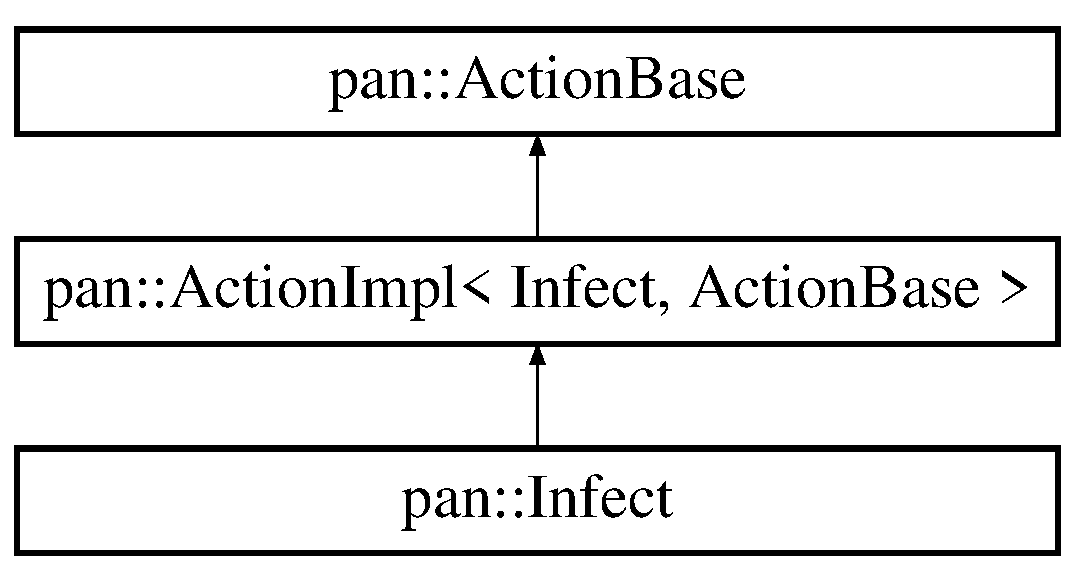
\includegraphics[height=3.000000cm]{classpan_1_1_infect}
\end{center}
\end{figure}
\subsection*{Public Member Functions}
\begin{DoxyCompactItemize}
\item 
\hyperlink{classpan_1_1_infect_ad6dfd4e6c39da420c65543f75c0e7d17}{Infect} (\hyperlink{namespacepan_afaed28aa6603153dcc062a028602d697}{City\+Index} \hyperlink{classpan_1_1_infect_a33fc44ae32daff748b39b2c787f2fb42}{city}, \hyperlink{namespacepan_a48851b51b0aef3f0e1be80df5031d9d7}{Disease\+Type} \hyperlink{classpan_1_1_infect_ad0a1d175916afcaf0f1050edf6536a97}{disease\+Type}, std\+::size\+\_\+t \hyperlink{classpan_1_1_infect_a3ad54add7a5021ba5fed764f8e688378}{cubes})
\end{DoxyCompactItemize}
\subsection*{Public Attributes}
\begin{DoxyCompactItemize}
\item 
\hyperlink{namespacepan_afaed28aa6603153dcc062a028602d697}{City\+Index} \hyperlink{classpan_1_1_infect_a33fc44ae32daff748b39b2c787f2fb42}{city}
\item 
std\+::size\+\_\+t \hyperlink{classpan_1_1_infect_a3ad54add7a5021ba5fed764f8e688378}{cubes}
\item 
\hyperlink{namespacepan_a48851b51b0aef3f0e1be80df5031d9d7}{Disease\+Type} \hyperlink{classpan_1_1_infect_ad0a1d175916afcaf0f1050edf6536a97}{disease\+Type}
\end{DoxyCompactItemize}


\subsection{Detailed Description}
Encapsulates the parameters of \hyperlink{classpan_1_1_infect}{Infect} call. 

\begin{DoxyAuthor}{Author}
Hrachya Hakobyan 
\end{DoxyAuthor}


\subsection{Constructor \& Destructor Documentation}
\mbox{\Hypertarget{classpan_1_1_infect_ad6dfd4e6c39da420c65543f75c0e7d17}\label{classpan_1_1_infect_ad6dfd4e6c39da420c65543f75c0e7d17}} 
\index{pan\+::\+Infect@{pan\+::\+Infect}!Infect@{Infect}}
\index{Infect@{Infect}!pan\+::\+Infect@{pan\+::\+Infect}}
\subsubsection{\texorpdfstring{Infect()}{Infect()}}
{\footnotesize\ttfamily pan\+::\+Infect\+::\+Infect (\begin{DoxyParamCaption}\item[{\hyperlink{namespacepan_afaed28aa6603153dcc062a028602d697}{City\+Index}}]{city,  }\item[{\hyperlink{namespacepan_a48851b51b0aef3f0e1be80df5031d9d7}{Disease\+Type}}]{disease\+Type,  }\item[{std\+::size\+\_\+t}]{cubes }\end{DoxyParamCaption})}



\subsection{Member Data Documentation}
\mbox{\Hypertarget{classpan_1_1_infect_a33fc44ae32daff748b39b2c787f2fb42}\label{classpan_1_1_infect_a33fc44ae32daff748b39b2c787f2fb42}} 
\index{pan\+::\+Infect@{pan\+::\+Infect}!city@{city}}
\index{city@{city}!pan\+::\+Infect@{pan\+::\+Infect}}
\subsubsection{\texorpdfstring{city}{city}}
{\footnotesize\ttfamily \hyperlink{namespacepan_afaed28aa6603153dcc062a028602d697}{City\+Index} pan\+::\+Infect\+::city}

The city to infect \mbox{\Hypertarget{classpan_1_1_infect_a3ad54add7a5021ba5fed764f8e688378}\label{classpan_1_1_infect_a3ad54add7a5021ba5fed764f8e688378}} 
\index{pan\+::\+Infect@{pan\+::\+Infect}!cubes@{cubes}}
\index{cubes@{cubes}!pan\+::\+Infect@{pan\+::\+Infect}}
\subsubsection{\texorpdfstring{cubes}{cubes}}
{\footnotesize\ttfamily std\+::size\+\_\+t pan\+::\+Infect\+::cubes}

How many cubes to put \mbox{\Hypertarget{classpan_1_1_infect_ad0a1d175916afcaf0f1050edf6536a97}\label{classpan_1_1_infect_ad0a1d175916afcaf0f1050edf6536a97}} 
\index{pan\+::\+Infect@{pan\+::\+Infect}!disease\+Type@{disease\+Type}}
\index{disease\+Type@{disease\+Type}!pan\+::\+Infect@{pan\+::\+Infect}}
\subsubsection{\texorpdfstring{disease\+Type}{diseaseType}}
{\footnotesize\ttfamily \hyperlink{namespacepan_a48851b51b0aef3f0e1be80df5031d9d7}{Disease\+Type} pan\+::\+Infect\+::disease\+Type}

The disease type of the cubes 

The documentation for this class was generated from the following files\+:\begin{DoxyCompactItemize}
\item 
\hyperlink{_infect_8h}{Infect.\+h}\item 
\hyperlink{_infect_8cpp}{Infect.\+cpp}\end{DoxyCompactItemize}

\hypertarget{classpan_1_1_map}{}\section{pan\+:\+:Map Class Reference}
\label{classpan_1_1_map}\index{pan\+::\+Map@{pan\+::\+Map}}


A class representing the game \hyperlink{classpan_1_1_map}{Map}, i.\+e. the board. Note, by the rules of the game the \hyperlink{classpan_1_1_map}{Map} requries at least one \hyperlink{classpan_1_1_region}{Region}. If one is not given, a default one will be constructed. The regions are implemented as a mapping between City\+Index-\/s and Region\+Index-\/s and Region\+Index-\/s and \hyperlink{classpan_1_1_region}{Region} objects.  




{\ttfamily \#include $<$Map.\+h$>$}

Inheritance diagram for pan\+:\+:Map\+:\begin{figure}[H]
\begin{center}
\leavevmode
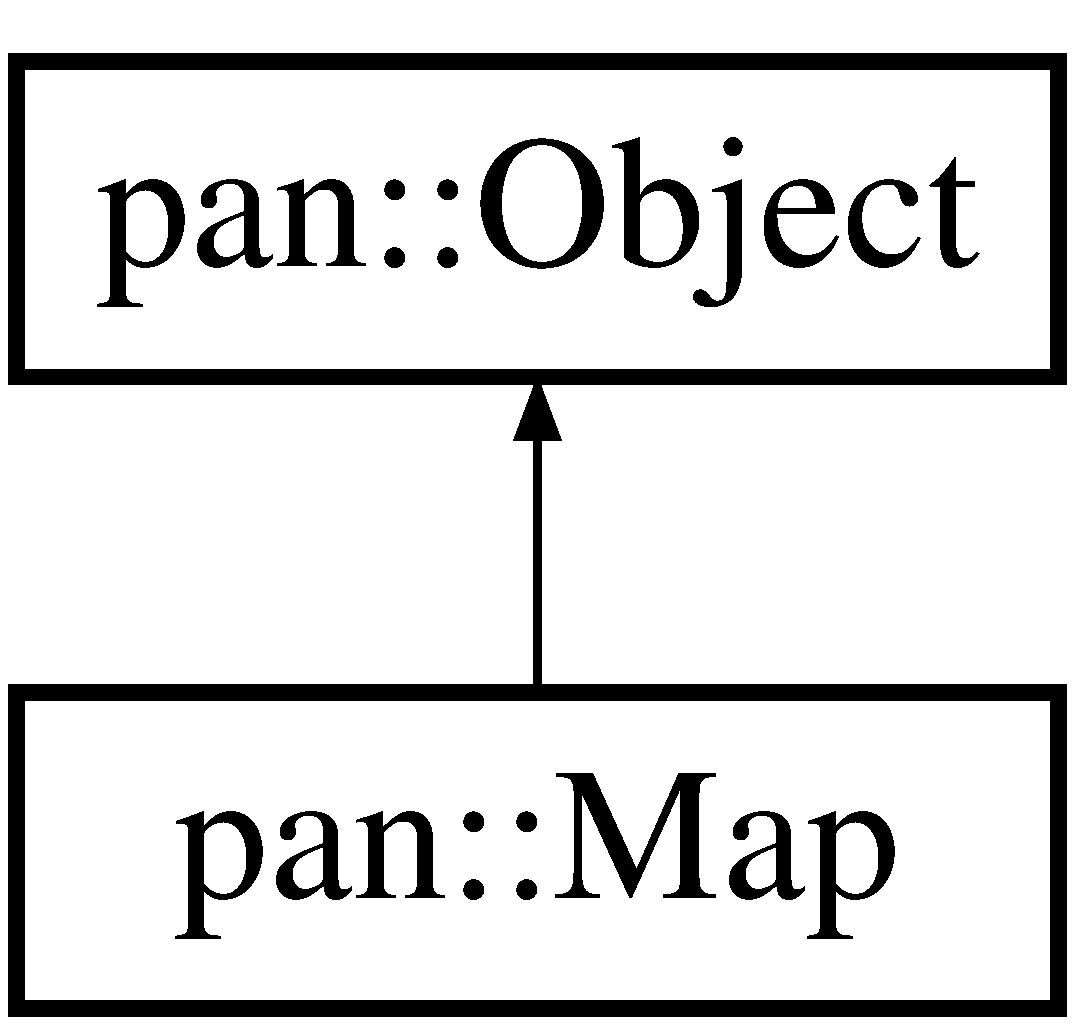
\includegraphics[height=2.000000cm]{classpan_1_1_map}
\end{center}
\end{figure}
\subsection*{Public Types}
\begin{DoxyCompactItemize}
\item 
typedef \hyperlink{classpan_1_1detail_1_1_graph}{detail\+::\+Graph}$<$ \hyperlink{classpan_1_1_city}{City} $>$\+::Vertex\+Iterator \hyperlink{classpan_1_1_map_a13baf12f486c6c3b823696266f06202c}{City\+Iterator}
\item 
typedef \hyperlink{classpan_1_1detail_1_1_graph}{detail\+::\+Graph}$<$ \hyperlink{classpan_1_1_city}{City} $>$\+::Adjacency\+Iterator \hyperlink{classpan_1_1_map_a616bc40b1a3f76f046be7ddf44ba90df}{Connected\+City\+Iterator}
\item 
typedef \hyperlink{classpan_1_1detail_1_1_graph}{detail\+::\+Graph}$<$ \hyperlink{classpan_1_1_city}{City} $>$\+::Adjacency\+Range \hyperlink{classpan_1_1_map_a6b1e81229ca2ed5c67202254948bde9b}{Connected\+City\+Range}
\end{DoxyCompactItemize}
\subsection*{Public Member Functions}
\begin{DoxyCompactItemize}
\item 
\hyperlink{classpan_1_1_map_a11ad1a3ad71e540b3f0c99f345e03e48}{Map} ()
\begin{DoxyCompactList}\small\item\em default constructor for \hyperlink{classpan_1_1_map}{Map}. Will create an initial region with index 0. \end{DoxyCompactList}\item 
\hyperlink{classpan_1_1_map_a60ce8e428c334ae75778774a46459128}{Map} (const \hyperlink{classpan_1_1_region}{Region} \&r)
\item 
\hyperlink{classpan_1_1_map_afe804f21ecea59695d8baabfb562026a}{Map} (const \hyperlink{classpan_1_1_map}{Map} \&)
\item 
\hyperlink{classpan_1_1_map_ac3348e336efab6436758eaa28c04db1a}{Map} (\hyperlink{classpan_1_1_map}{Map} \&\&)
\item 
\hyperlink{classpan_1_1_map}{Map} \& \hyperlink{classpan_1_1_map_af9d36a347d38a376d5da72bf85e95f68}{operator=} (const \hyperlink{classpan_1_1_map}{Map} \&)
\item 
\hyperlink{classpan_1_1_map}{Map} \& \hyperlink{classpan_1_1_map_a3413513964774303b47161eb8ed922f8}{operator=} (\hyperlink{classpan_1_1_map}{Map} \&\&)
\item 
\hyperlink{classpan_1_1_map_a91d7bff34d75bc416ec7e6bdc4a497ab}{$\sim$\+Map} ()=default
\item 
bool \hyperlink{classpan_1_1_map_a7b06691976776c099e60890b15b4eb99}{operator==} (const \hyperlink{classpan_1_1_map}{Map} \&other) const
\item 
bool \hyperlink{classpan_1_1_map_a7f5b4f8589dd3a4951e35d198b4f8048}{operator!=} (const \hyperlink{classpan_1_1_map}{Map} \&other) const
\item 
{\footnotesize template$<$class Archive $>$ }\\void \hyperlink{classpan_1_1_map_a0afa3368bc2f5fbd85b4b2c3205f0996}{serialize} (Archive \&ar, const unsigned int)
\item 
std\+::string \hyperlink{classpan_1_1_map_a9d08be170f445bbef11ea0d38ba8c531}{description} () const
\item 
std\+::size\+\_\+t \hyperlink{classpan_1_1_map_aa39642daa76646a3229fd5f92572b242}{num\+Cities} () const
\item 
std\+::size\+\_\+t \hyperlink{classpan_1_1_map_a70b6a65dc76e8911beb524062a2d09a9}{num\+Connections} () const
\item 
bool \hyperlink{classpan_1_1_map_a331d27d9fe199aea61b6ed76b4950d55}{city\+Exists} (\hyperlink{namespacepan_afaed28aa6603153dcc062a028602d697}{City\+Index} i) const
\item 
const \hyperlink{classpan_1_1_city}{City} \& \hyperlink{classpan_1_1_map_a0f7820b581ca27511a687618f01dce2d}{operator\mbox{[}$\,$\mbox{]}} (\hyperlink{namespacepan_afaed28aa6603153dcc062a028602d697}{City\+Index} i) const
\item 
\hyperlink{classpan_1_1_city}{City} \& \hyperlink{classpan_1_1_map_ab9e03b7854710fdbd279e62c2494ef06}{operator\mbox{[}$\,$\mbox{]}} (\hyperlink{namespacepan_afaed28aa6603153dcc062a028602d697}{City\+Index} i)
\item 
bool \hyperlink{classpan_1_1_map_ae6644155d9ddd28d82ab393e62024637}{connection\+Exists} (\hyperlink{namespacepan_afaed28aa6603153dcc062a028602d697}{City\+Index} i, \hyperlink{namespacepan_afaed28aa6603153dcc062a028602d697}{City\+Index} j) const
\item 
\hyperlink{classpan_1_1_map_a6b1e81229ca2ed5c67202254948bde9b}{Connected\+City\+Range} \hyperlink{classpan_1_1_map_a1cb8308c1ddac316a683be688277a25a}{connected\+Cities} (\hyperlink{namespacepan_afaed28aa6603153dcc062a028602d697}{City\+Index} i) const
\item 
std\+::size\+\_\+t \hyperlink{classpan_1_1_map_a7e61225a4309562a5b8df58acb325276}{num\+Regions} () const
\item 
std\+::vector$<$ \hyperlink{namespacepan_a648dcc32a76222a9e4cd4a3e80bda642}{Region\+Index} $>$ \hyperlink{classpan_1_1_map_a580c57ef43aaf9c4c964d18340754d3c}{get\+Regions} () const
\item 
const \hyperlink{classpan_1_1_region}{Region} \& \hyperlink{classpan_1_1_map_ac0597ceffd926725744a6518c7773421}{region\+At} (\hyperlink{namespacepan_a648dcc32a76222a9e4cd4a3e80bda642}{Region\+Index} index) const
\item 
\hyperlink{namespacepan_a648dcc32a76222a9e4cd4a3e80bda642}{Region\+Index} \hyperlink{classpan_1_1_map_af477415a73c3e1fed14f1bd3753da6b1}{region\+For\+City} (\hyperlink{namespacepan_afaed28aa6603153dcc062a028602d697}{City\+Index} i) const
\item 
std\+::set$<$ \hyperlink{namespacepan_afaed28aa6603153dcc062a028602d697}{City\+Index} $>$ \hyperlink{classpan_1_1_map_a6c28ef7bcc328fa4260309aa14f50f8a}{region\+Cities} (\hyperlink{namespacepan_a648dcc32a76222a9e4cd4a3e80bda642}{Region\+Index} index) const
\end{DoxyCompactItemize}
\subsection*{Static Public Member Functions}
\begin{DoxyCompactItemize}
\item 
static \hyperlink{classpan_1_1_map}{Map} \hyperlink{classpan_1_1_map_afc16b42064eca43b341cd4a555bed092}{pandemic\+Map} ()
\end{DoxyCompactItemize}
\subsection*{Friends}
\begin{DoxyCompactItemize}
\item 
class \hyperlink{classpan_1_1_map_ac98d07dd8f7b70e16ccb9a01abf56b9c}{boost\+::serialization\+::access}
\end{DoxyCompactItemize}


\subsection{Detailed Description}
A class representing the game \hyperlink{classpan_1_1_map}{Map}, i.\+e. the board. Note, by the rules of the game the \hyperlink{classpan_1_1_map}{Map} requries at least one \hyperlink{classpan_1_1_region}{Region}. If one is not given, a default one will be constructed. The regions are implemented as a mapping between City\+Index-\/s and Region\+Index-\/s and Region\+Index-\/s and \hyperlink{classpan_1_1_region}{Region} objects. 

\begin{DoxyAuthor}{Author}
Hrachya Hakobyan 
\end{DoxyAuthor}


\subsection{Member Typedef Documentation}
\mbox{\Hypertarget{classpan_1_1_map_a13baf12f486c6c3b823696266f06202c}\label{classpan_1_1_map_a13baf12f486c6c3b823696266f06202c}} 
\index{pan\+::\+Map@{pan\+::\+Map}!City\+Iterator@{City\+Iterator}}
\index{City\+Iterator@{City\+Iterator}!pan\+::\+Map@{pan\+::\+Map}}
\subsubsection{\texorpdfstring{City\+Iterator}{CityIterator}}
{\footnotesize\ttfamily typedef \hyperlink{classpan_1_1detail_1_1_graph}{detail\+::\+Graph}$<$\hyperlink{classpan_1_1_city}{City}$>$\+::Vertex\+Iterator \hyperlink{classpan_1_1_map_a13baf12f486c6c3b823696266f06202c}{pan\+::\+Map\+::\+City\+Iterator}}

\mbox{\Hypertarget{classpan_1_1_map_a616bc40b1a3f76f046be7ddf44ba90df}\label{classpan_1_1_map_a616bc40b1a3f76f046be7ddf44ba90df}} 
\index{pan\+::\+Map@{pan\+::\+Map}!Connected\+City\+Iterator@{Connected\+City\+Iterator}}
\index{Connected\+City\+Iterator@{Connected\+City\+Iterator}!pan\+::\+Map@{pan\+::\+Map}}
\subsubsection{\texorpdfstring{Connected\+City\+Iterator}{ConnectedCityIterator}}
{\footnotesize\ttfamily typedef \hyperlink{classpan_1_1detail_1_1_graph}{detail\+::\+Graph}$<$\hyperlink{classpan_1_1_city}{City}$>$\+::Adjacency\+Iterator \hyperlink{classpan_1_1_map_a616bc40b1a3f76f046be7ddf44ba90df}{pan\+::\+Map\+::\+Connected\+City\+Iterator}}

\mbox{\Hypertarget{classpan_1_1_map_a6b1e81229ca2ed5c67202254948bde9b}\label{classpan_1_1_map_a6b1e81229ca2ed5c67202254948bde9b}} 
\index{pan\+::\+Map@{pan\+::\+Map}!Connected\+City\+Range@{Connected\+City\+Range}}
\index{Connected\+City\+Range@{Connected\+City\+Range}!pan\+::\+Map@{pan\+::\+Map}}
\subsubsection{\texorpdfstring{Connected\+City\+Range}{ConnectedCityRange}}
{\footnotesize\ttfamily typedef \hyperlink{classpan_1_1detail_1_1_graph}{detail\+::\+Graph}$<$\hyperlink{classpan_1_1_city}{City}$>$\+::Adjacency\+Range \hyperlink{classpan_1_1_map_a6b1e81229ca2ed5c67202254948bde9b}{pan\+::\+Map\+::\+Connected\+City\+Range}}



\subsection{Constructor \& Destructor Documentation}
\mbox{\Hypertarget{classpan_1_1_map_a11ad1a3ad71e540b3f0c99f345e03e48}\label{classpan_1_1_map_a11ad1a3ad71e540b3f0c99f345e03e48}} 
\index{pan\+::\+Map@{pan\+::\+Map}!Map@{Map}}
\index{Map@{Map}!pan\+::\+Map@{pan\+::\+Map}}
\subsubsection{\texorpdfstring{Map()}{Map()}\hspace{0.1cm}{\footnotesize\ttfamily [1/4]}}
{\footnotesize\ttfamily pan\+::\+Map\+::\+Map (\begin{DoxyParamCaption}{ }\end{DoxyParamCaption})}



default constructor for \hyperlink{classpan_1_1_map}{Map}. Will create an initial region with index 0. 

\mbox{\Hypertarget{classpan_1_1_map_a60ce8e428c334ae75778774a46459128}\label{classpan_1_1_map_a60ce8e428c334ae75778774a46459128}} 
\index{pan\+::\+Map@{pan\+::\+Map}!Map@{Map}}
\index{Map@{Map}!pan\+::\+Map@{pan\+::\+Map}}
\subsubsection{\texorpdfstring{Map()}{Map()}\hspace{0.1cm}{\footnotesize\ttfamily [2/4]}}
{\footnotesize\ttfamily pan\+::\+Map\+::\+Map (\begin{DoxyParamCaption}\item[{const \hyperlink{classpan_1_1_region}{Region} \&}]{r }\end{DoxyParamCaption})\hspace{0.3cm}{\ttfamily [explicit]}}

\mbox{\Hypertarget{classpan_1_1_map_afe804f21ecea59695d8baabfb562026a}\label{classpan_1_1_map_afe804f21ecea59695d8baabfb562026a}} 
\index{pan\+::\+Map@{pan\+::\+Map}!Map@{Map}}
\index{Map@{Map}!pan\+::\+Map@{pan\+::\+Map}}
\subsubsection{\texorpdfstring{Map()}{Map()}\hspace{0.1cm}{\footnotesize\ttfamily [3/4]}}
{\footnotesize\ttfamily pan\+::\+Map\+::\+Map (\begin{DoxyParamCaption}\item[{const \hyperlink{classpan_1_1_map}{Map} \&}]{o }\end{DoxyParamCaption})}

\mbox{\Hypertarget{classpan_1_1_map_ac3348e336efab6436758eaa28c04db1a}\label{classpan_1_1_map_ac3348e336efab6436758eaa28c04db1a}} 
\index{pan\+::\+Map@{pan\+::\+Map}!Map@{Map}}
\index{Map@{Map}!pan\+::\+Map@{pan\+::\+Map}}
\subsubsection{\texorpdfstring{Map()}{Map()}\hspace{0.1cm}{\footnotesize\ttfamily [4/4]}}
{\footnotesize\ttfamily pan\+::\+Map\+::\+Map (\begin{DoxyParamCaption}\item[{\hyperlink{classpan_1_1_map}{Map} \&\&}]{o }\end{DoxyParamCaption})}

\mbox{\Hypertarget{classpan_1_1_map_a91d7bff34d75bc416ec7e6bdc4a497ab}\label{classpan_1_1_map_a91d7bff34d75bc416ec7e6bdc4a497ab}} 
\index{pan\+::\+Map@{pan\+::\+Map}!````~Map@{$\sim$\+Map}}
\index{````~Map@{$\sim$\+Map}!pan\+::\+Map@{pan\+::\+Map}}
\subsubsection{\texorpdfstring{$\sim$\+Map()}{~Map()}}
{\footnotesize\ttfamily pan\+::\+Map\+::$\sim$\+Map (\begin{DoxyParamCaption}{ }\end{DoxyParamCaption})\hspace{0.3cm}{\ttfamily [default]}}



\subsection{Member Function Documentation}
\mbox{\Hypertarget{classpan_1_1_map_a331d27d9fe199aea61b6ed76b4950d55}\label{classpan_1_1_map_a331d27d9fe199aea61b6ed76b4950d55}} 
\index{pan\+::\+Map@{pan\+::\+Map}!city\+Exists@{city\+Exists}}
\index{city\+Exists@{city\+Exists}!pan\+::\+Map@{pan\+::\+Map}}
\subsubsection{\texorpdfstring{city\+Exists()}{cityExists()}}
{\footnotesize\ttfamily bool pan\+::\+Map\+::city\+Exists (\begin{DoxyParamCaption}\item[{\hyperlink{namespacepan_afaed28aa6603153dcc062a028602d697}{City\+Index}}]{i }\end{DoxyParamCaption}) const\hspace{0.3cm}{\ttfamily [inline]}}

Checks if a city exists. 
\begin{DoxyParams}{Parameters}
{\em index} & the City\+Index to be checked \\
\hline
\end{DoxyParams}
\begin{DoxyReturn}{Returns}
true if the city exists, false otherwise 
\end{DoxyReturn}
\mbox{\Hypertarget{classpan_1_1_map_a1cb8308c1ddac316a683be688277a25a}\label{classpan_1_1_map_a1cb8308c1ddac316a683be688277a25a}} 
\index{pan\+::\+Map@{pan\+::\+Map}!connected\+Cities@{connected\+Cities}}
\index{connected\+Cities@{connected\+Cities}!pan\+::\+Map@{pan\+::\+Map}}
\subsubsection{\texorpdfstring{connected\+Cities()}{connectedCities()}}
{\footnotesize\ttfamily \hyperlink{classpan_1_1_map_a6b1e81229ca2ed5c67202254948bde9b}{Map\+::\+Connected\+City\+Range} pan\+::\+Map\+::connected\+Cities (\begin{DoxyParamCaption}\item[{\hyperlink{namespacepan_afaed28aa6603153dcc062a028602d697}{City\+Index}}]{i }\end{DoxyParamCaption}) const\hspace{0.3cm}{\ttfamily [inline]}}

Returns the connected cities. 
\begin{DoxyParams}{Parameters}
{\em i} & the city index \\
\hline
\end{DoxyParams}

\begin{DoxyExceptions}{Exceptions}
{\em std\+::exception} & if index is invalid \\
\hline
\end{DoxyExceptions}
\begin{DoxyReturn}{Returns}
iterator pair for the neighbor cities of i 
\end{DoxyReturn}
\mbox{\Hypertarget{classpan_1_1_map_ae6644155d9ddd28d82ab393e62024637}\label{classpan_1_1_map_ae6644155d9ddd28d82ab393e62024637}} 
\index{pan\+::\+Map@{pan\+::\+Map}!connection\+Exists@{connection\+Exists}}
\index{connection\+Exists@{connection\+Exists}!pan\+::\+Map@{pan\+::\+Map}}
\subsubsection{\texorpdfstring{connection\+Exists()}{connectionExists()}}
{\footnotesize\ttfamily bool pan\+::\+Map\+::connection\+Exists (\begin{DoxyParamCaption}\item[{\hyperlink{namespacepan_afaed28aa6603153dcc062a028602d697}{City\+Index}}]{i,  }\item[{\hyperlink{namespacepan_afaed28aa6603153dcc062a028602d697}{City\+Index}}]{j }\end{DoxyParamCaption}) const\hspace{0.3cm}{\ttfamily [inline]}}

Checks if cities at specified indeces are connected/ 
\begin{DoxyParams}{Parameters}
{\em i} & the index of the first \hyperlink{classpan_1_1_city}{City} \\
\hline
{\em j} & the index of the second \hyperlink{classpan_1_1_city}{City} \\
\hline
\end{DoxyParams}
\begin{DoxyReturn}{Returns}
true if a connection between the cities exists, false otherwise 
\end{DoxyReturn}
\mbox{\Hypertarget{classpan_1_1_map_a9d08be170f445bbef11ea0d38ba8c531}\label{classpan_1_1_map_a9d08be170f445bbef11ea0d38ba8c531}} 
\index{pan\+::\+Map@{pan\+::\+Map}!description@{description}}
\index{description@{description}!pan\+::\+Map@{pan\+::\+Map}}
\subsubsection{\texorpdfstring{description()}{description()}}
{\footnotesize\ttfamily std\+::string pan\+::\+Map\+::description (\begin{DoxyParamCaption}{ }\end{DoxyParamCaption}) const\hspace{0.3cm}{\ttfamily [virtual]}}

Public Interaface 

Implements \hyperlink{classpan_1_1_object_a2bb6d3117bb32f5774657c83f118ed8b}{pan\+::\+Object}.

\mbox{\Hypertarget{classpan_1_1_map_a580c57ef43aaf9c4c964d18340754d3c}\label{classpan_1_1_map_a580c57ef43aaf9c4c964d18340754d3c}} 
\index{pan\+::\+Map@{pan\+::\+Map}!get\+Regions@{get\+Regions}}
\index{get\+Regions@{get\+Regions}!pan\+::\+Map@{pan\+::\+Map}}
\subsubsection{\texorpdfstring{get\+Regions()}{getRegions()}}
{\footnotesize\ttfamily std\+::vector$<$ \hyperlink{namespacepan_a648dcc32a76222a9e4cd4a3e80bda642}{Region\+Index} $>$ pan\+::\+Map\+::get\+Regions (\begin{DoxyParamCaption}{ }\end{DoxyParamCaption}) const}

Returns all regions in the map. \begin{DoxyReturn}{Returns}
vector of all regions in the map. 
\end{DoxyReturn}
\mbox{\Hypertarget{classpan_1_1_map_aa39642daa76646a3229fd5f92572b242}\label{classpan_1_1_map_aa39642daa76646a3229fd5f92572b242}} 
\index{pan\+::\+Map@{pan\+::\+Map}!num\+Cities@{num\+Cities}}
\index{num\+Cities@{num\+Cities}!pan\+::\+Map@{pan\+::\+Map}}
\subsubsection{\texorpdfstring{num\+Cities()}{numCities()}}
{\footnotesize\ttfamily std\+::size\+\_\+t pan\+::\+Map\+::num\+Cities (\begin{DoxyParamCaption}{ }\end{DoxyParamCaption}) const\hspace{0.3cm}{\ttfamily [inline]}}

Getter for the number of cities. \begin{DoxyReturn}{Returns}
the number of cities on the map
\end{DoxyReturn}
Public Interface \mbox{\Hypertarget{classpan_1_1_map_a70b6a65dc76e8911beb524062a2d09a9}\label{classpan_1_1_map_a70b6a65dc76e8911beb524062a2d09a9}} 
\index{pan\+::\+Map@{pan\+::\+Map}!num\+Connections@{num\+Connections}}
\index{num\+Connections@{num\+Connections}!pan\+::\+Map@{pan\+::\+Map}}
\subsubsection{\texorpdfstring{num\+Connections()}{numConnections()}}
{\footnotesize\ttfamily std\+::size\+\_\+t pan\+::\+Map\+::num\+Connections (\begin{DoxyParamCaption}{ }\end{DoxyParamCaption}) const\hspace{0.3cm}{\ttfamily [inline]}}

Getter for the number of connections. \begin{DoxyReturn}{Returns}
the number of connections, i.\+e. edges on the map. 
\end{DoxyReturn}
\mbox{\Hypertarget{classpan_1_1_map_a7e61225a4309562a5b8df58acb325276}\label{classpan_1_1_map_a7e61225a4309562a5b8df58acb325276}} 
\index{pan\+::\+Map@{pan\+::\+Map}!num\+Regions@{num\+Regions}}
\index{num\+Regions@{num\+Regions}!pan\+::\+Map@{pan\+::\+Map}}
\subsubsection{\texorpdfstring{num\+Regions()}{numRegions()}}
{\footnotesize\ttfamily std\+::size\+\_\+t pan\+::\+Map\+::num\+Regions (\begin{DoxyParamCaption}{ }\end{DoxyParamCaption}) const\hspace{0.3cm}{\ttfamily [inline]}}

Returns the number of regions in the map. \begin{DoxyReturn}{Returns}
the number of regions on the map 
\end{DoxyReturn}
\mbox{\Hypertarget{classpan_1_1_map_a7f5b4f8589dd3a4951e35d198b4f8048}\label{classpan_1_1_map_a7f5b4f8589dd3a4951e35d198b4f8048}} 
\index{pan\+::\+Map@{pan\+::\+Map}!operator"!=@{operator"!=}}
\index{operator"!=@{operator"!=}!pan\+::\+Map@{pan\+::\+Map}}
\subsubsection{\texorpdfstring{operator"!=()}{operator!=()}}
{\footnotesize\ttfamily bool pan\+::\+Map\+::operator!= (\begin{DoxyParamCaption}\item[{const \hyperlink{classpan_1_1_map}{Map} \&}]{other }\end{DoxyParamCaption}) const\hspace{0.3cm}{\ttfamily [inline]}}

\mbox{\Hypertarget{classpan_1_1_map_af9d36a347d38a376d5da72bf85e95f68}\label{classpan_1_1_map_af9d36a347d38a376d5da72bf85e95f68}} 
\index{pan\+::\+Map@{pan\+::\+Map}!operator=@{operator=}}
\index{operator=@{operator=}!pan\+::\+Map@{pan\+::\+Map}}
\subsubsection{\texorpdfstring{operator=()}{operator=()}\hspace{0.1cm}{\footnotesize\ttfamily [1/2]}}
{\footnotesize\ttfamily \hyperlink{classpan_1_1_map}{Map} \& pan\+::\+Map\+::operator= (\begin{DoxyParamCaption}\item[{const \hyperlink{classpan_1_1_map}{Map} \&}]{o }\end{DoxyParamCaption})}

\mbox{\Hypertarget{classpan_1_1_map_a3413513964774303b47161eb8ed922f8}\label{classpan_1_1_map_a3413513964774303b47161eb8ed922f8}} 
\index{pan\+::\+Map@{pan\+::\+Map}!operator=@{operator=}}
\index{operator=@{operator=}!pan\+::\+Map@{pan\+::\+Map}}
\subsubsection{\texorpdfstring{operator=()}{operator=()}\hspace{0.1cm}{\footnotesize\ttfamily [2/2]}}
{\footnotesize\ttfamily \hyperlink{classpan_1_1_map}{Map} \& pan\+::\+Map\+::operator= (\begin{DoxyParamCaption}\item[{\hyperlink{classpan_1_1_map}{Map} \&\&}]{o }\end{DoxyParamCaption})}

\mbox{\Hypertarget{classpan_1_1_map_a7b06691976776c099e60890b15b4eb99}\label{classpan_1_1_map_a7b06691976776c099e60890b15b4eb99}} 
\index{pan\+::\+Map@{pan\+::\+Map}!operator==@{operator==}}
\index{operator==@{operator==}!pan\+::\+Map@{pan\+::\+Map}}
\subsubsection{\texorpdfstring{operator==()}{operator==()}}
{\footnotesize\ttfamily bool pan\+::\+Map\+::operator== (\begin{DoxyParamCaption}\item[{const \hyperlink{classpan_1_1_map}{Map} \&}]{other }\end{DoxyParamCaption}) const}

Comparison operators. Note, full fledged comparison is not feasible (i.\+e. graph isomorphism). The comparison does not take into account edge connectivity of the cities. \mbox{\Hypertarget{classpan_1_1_map_a0f7820b581ca27511a687618f01dce2d}\label{classpan_1_1_map_a0f7820b581ca27511a687618f01dce2d}} 
\index{pan\+::\+Map@{pan\+::\+Map}!operator\mbox{[}\mbox{]}@{operator[]}}
\index{operator\mbox{[}\mbox{]}@{operator[]}!pan\+::\+Map@{pan\+::\+Map}}
\subsubsection{\texorpdfstring{operator[]()}{operator[]()}\hspace{0.1cm}{\footnotesize\ttfamily [1/2]}}
{\footnotesize\ttfamily const \hyperlink{classpan_1_1_city}{City} \& pan\+::\+Map\+::operator\mbox{[}$\,$\mbox{]} (\begin{DoxyParamCaption}\item[{\hyperlink{namespacepan_afaed28aa6603153dcc062a028602d697}{City\+Index}}]{i }\end{DoxyParamCaption}) const\hspace{0.3cm}{\ttfamily [inline]}}

Returns the const reference of the \hyperlink{classpan_1_1_city}{City} object at the corresponding index. 
\begin{DoxyParams}{Parameters}
{\em i} & the City\+Index of the reference of the object to be returned \\
\hline
\end{DoxyParams}

\begin{DoxyExceptions}{Exceptions}
{\em std\+::exception} & if the index in invalid \\
\hline
\end{DoxyExceptions}
\begin{DoxyReturn}{Returns}
the constant reference of the \hyperlink{classpan_1_1_city}{City} object at the specified index 
\end{DoxyReturn}
\mbox{\Hypertarget{classpan_1_1_map_ab9e03b7854710fdbd279e62c2494ef06}\label{classpan_1_1_map_ab9e03b7854710fdbd279e62c2494ef06}} 
\index{pan\+::\+Map@{pan\+::\+Map}!operator\mbox{[}\mbox{]}@{operator[]}}
\index{operator\mbox{[}\mbox{]}@{operator[]}!pan\+::\+Map@{pan\+::\+Map}}
\subsubsection{\texorpdfstring{operator[]()}{operator[]()}\hspace{0.1cm}{\footnotesize\ttfamily [2/2]}}
{\footnotesize\ttfamily \hyperlink{classpan_1_1_city}{City} \& pan\+::\+Map\+::operator\mbox{[}$\,$\mbox{]} (\begin{DoxyParamCaption}\item[{\hyperlink{namespacepan_afaed28aa6603153dcc062a028602d697}{City\+Index}}]{i }\end{DoxyParamCaption})\hspace{0.3cm}{\ttfamily [inline]}}

Returns the reference of the \hyperlink{classpan_1_1_city}{City} object at the corresponding index. 
\begin{DoxyParams}{Parameters}
{\em i} & the City\+Index of the reference of the object to be returned \\
\hline
\end{DoxyParams}

\begin{DoxyExceptions}{Exceptions}
{\em std\+::exception} & if the index is invalid \\
\hline
\end{DoxyExceptions}
\begin{DoxyReturn}{Returns}
the reference of the \hyperlink{classpan_1_1_city}{City} object at the specified index 
\end{DoxyReturn}
\mbox{\Hypertarget{classpan_1_1_map_afc16b42064eca43b341cd4a555bed092}\label{classpan_1_1_map_afc16b42064eca43b341cd4a555bed092}} 
\index{pan\+::\+Map@{pan\+::\+Map}!pandemic\+Map@{pandemic\+Map}}
\index{pandemic\+Map@{pandemic\+Map}!pan\+::\+Map@{pan\+::\+Map}}
\subsubsection{\texorpdfstring{pandemic\+Map()}{pandemicMap()}}
{\footnotesize\ttfamily \hyperlink{classpan_1_1_map}{Map} pan\+::\+Map\+::pandemic\+Map (\begin{DoxyParamCaption}{ }\end{DoxyParamCaption})\hspace{0.3cm}{\ttfamily [static]}}

\mbox{\Hypertarget{classpan_1_1_map_ac0597ceffd926725744a6518c7773421}\label{classpan_1_1_map_ac0597ceffd926725744a6518c7773421}} 
\index{pan\+::\+Map@{pan\+::\+Map}!region\+At@{region\+At}}
\index{region\+At@{region\+At}!pan\+::\+Map@{pan\+::\+Map}}
\subsubsection{\texorpdfstring{region\+At()}{regionAt()}}
{\footnotesize\ttfamily const \hyperlink{classpan_1_1_region}{Region} \& pan\+::\+Map\+::region\+At (\begin{DoxyParamCaption}\item[{\hyperlink{namespacepan_a648dcc32a76222a9e4cd4a3e80bda642}{Region\+Index}}]{index }\end{DoxyParamCaption}) const\hspace{0.3cm}{\ttfamily [inline]}}

Returns the region with the specified index. 
\begin{DoxyParams}{Parameters}
{\em index} & the index of the \hyperlink{classpan_1_1_region}{Region} \\
\hline
\end{DoxyParams}

\begin{DoxyExceptions}{Exceptions}
{\em std\+::exception} & if the index is invalid \\
\hline
\end{DoxyExceptions}
\begin{DoxyReturn}{Returns}
the const reference to the specified \hyperlink{classpan_1_1_region}{Region} 
\end{DoxyReturn}
\mbox{\Hypertarget{classpan_1_1_map_a6c28ef7bcc328fa4260309aa14f50f8a}\label{classpan_1_1_map_a6c28ef7bcc328fa4260309aa14f50f8a}} 
\index{pan\+::\+Map@{pan\+::\+Map}!region\+Cities@{region\+Cities}}
\index{region\+Cities@{region\+Cities}!pan\+::\+Map@{pan\+::\+Map}}
\subsubsection{\texorpdfstring{region\+Cities()}{regionCities()}}
{\footnotesize\ttfamily std\+::set$<$ \hyperlink{namespacepan_afaed28aa6603153dcc062a028602d697}{City\+Index} $>$ pan\+::\+Map\+::region\+Cities (\begin{DoxyParamCaption}\item[{\hyperlink{namespacepan_a648dcc32a76222a9e4cd4a3e80bda642}{Region\+Index}}]{index }\end{DoxyParamCaption}) const}

Returns the City\+Index-\/s of the specified \hyperlink{classpan_1_1_region}{Region} Caution, O(\+N) operation on the number of vertices. 
\begin{DoxyParams}{Parameters}
{\em index} & the index of the region \\
\hline
\end{DoxyParams}

\begin{DoxyExceptions}{Exceptions}
{\em std\+::exception} & if the index is invalid \\
\hline
\end{DoxyExceptions}
\begin{DoxyReturn}{Returns}
the set of City\+Index-\/s of the region 
\end{DoxyReturn}
\mbox{\Hypertarget{classpan_1_1_map_af477415a73c3e1fed14f1bd3753da6b1}\label{classpan_1_1_map_af477415a73c3e1fed14f1bd3753da6b1}} 
\index{pan\+::\+Map@{pan\+::\+Map}!region\+For\+City@{region\+For\+City}}
\index{region\+For\+City@{region\+For\+City}!pan\+::\+Map@{pan\+::\+Map}}
\subsubsection{\texorpdfstring{region\+For\+City()}{regionForCity()}}
{\footnotesize\ttfamily \hyperlink{namespacepan_a648dcc32a76222a9e4cd4a3e80bda642}{Region\+Index} pan\+::\+Map\+::region\+For\+City (\begin{DoxyParamCaption}\item[{\hyperlink{namespacepan_afaed28aa6603153dcc062a028602d697}{City\+Index}}]{i }\end{DoxyParamCaption}) const}

Returns the region of the city with the specified City\+Index 
\begin{DoxyParams}{Parameters}
{\em index} & the index of the city \\
\hline
\end{DoxyParams}

\begin{DoxyExceptions}{Exceptions}
{\em std\+::exception} & if the index is invalid \\
\hline
\end{DoxyExceptions}
\begin{DoxyReturn}{Returns}
the const reference to the \hyperlink{classpan_1_1_region}{Region} of the city 
\end{DoxyReturn}
\mbox{\Hypertarget{classpan_1_1_map_a0afa3368bc2f5fbd85b4b2c3205f0996}\label{classpan_1_1_map_a0afa3368bc2f5fbd85b4b2c3205f0996}} 
\index{pan\+::\+Map@{pan\+::\+Map}!serialize@{serialize}}
\index{serialize@{serialize}!pan\+::\+Map@{pan\+::\+Map}}
\subsubsection{\texorpdfstring{serialize()}{serialize()}}
{\footnotesize\ttfamily template$<$class Archive $>$ \\
void pan\+::\+Map\+::serialize (\begin{DoxyParamCaption}\item[{Archive \&}]{ar,  }\item[{const unsigned}]{int }\end{DoxyParamCaption})\hspace{0.3cm}{\ttfamily [inline]}}



\subsection{Friends And Related Function Documentation}
\mbox{\Hypertarget{classpan_1_1_map_ac98d07dd8f7b70e16ccb9a01abf56b9c}\label{classpan_1_1_map_ac98d07dd8f7b70e16ccb9a01abf56b9c}} 
\index{pan\+::\+Map@{pan\+::\+Map}!boost\+::serialization\+::access@{boost\+::serialization\+::access}}
\index{boost\+::serialization\+::access@{boost\+::serialization\+::access}!pan\+::\+Map@{pan\+::\+Map}}
\subsubsection{\texorpdfstring{boost\+::serialization\+::access}{boost::serialization::access}}
{\footnotesize\ttfamily friend class boost\+::serialization\+::access\hspace{0.3cm}{\ttfamily [friend]}}



The documentation for this class was generated from the following files\+:\begin{DoxyCompactItemize}
\item 
\hyperlink{_map_8h}{Map.\+h}\item 
\hyperlink{_map_8cpp}{Map.\+cpp}\end{DoxyCompactItemize}

\hypertarget{classpan_1_1_move}{}\section{pan\+:\+:Move Class Reference}
\label{classpan_1_1_move}\index{pan\+::\+Move@{pan\+::\+Move}}


Class representing a driver/ferry action.  




{\ttfamily \#include $<$Move.\+h$>$}

Inheritance diagram for pan\+:\+:Move\+:\begin{figure}[H]
\begin{center}
\leavevmode
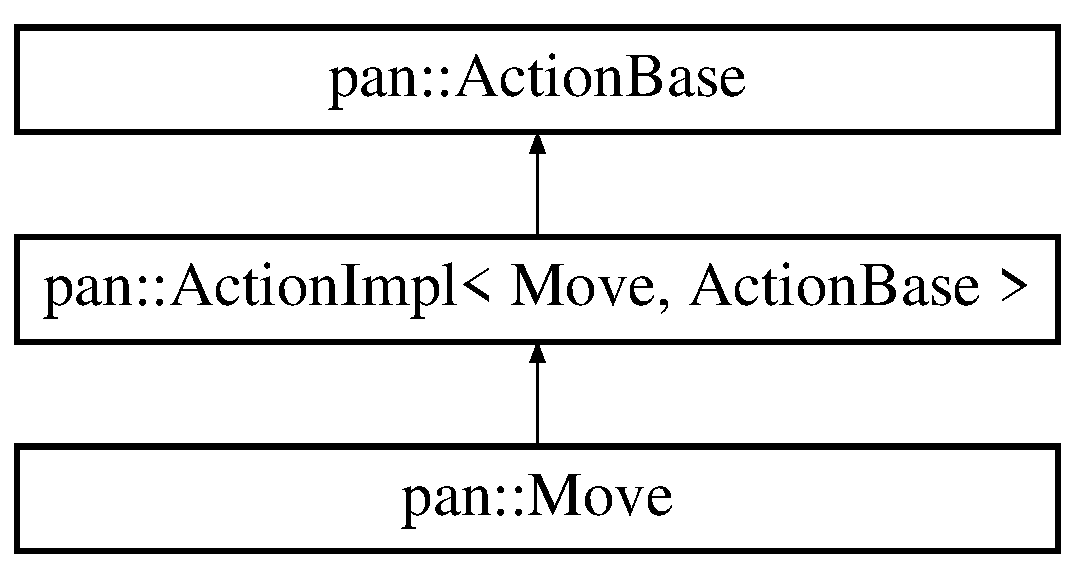
\includegraphics[height=3.000000cm]{classpan_1_1_move}
\end{center}
\end{figure}
\subsection*{Public Member Functions}
\begin{DoxyCompactItemize}
\item 
\hyperlink{classpan_1_1_move_a4e08c8a5412da98cef5e70b5e30d8cc5}{Move} (\hyperlink{namespacepan_a0cdabf874fbf1bb3a1f0152d108c2909}{Player\+Index} \hyperlink{classpan_1_1_move_a56c9b18c1a51462ca1bcf777e2f45bbd}{player}, \hyperlink{namespacepan_afaed28aa6603153dcc062a028602d697}{City\+Index} city)
\end{DoxyCompactItemize}
\subsection*{Public Attributes}
\begin{DoxyCompactItemize}
\item 
\hyperlink{namespacepan_a0cdabf874fbf1bb3a1f0152d108c2909}{Player\+Index} \hyperlink{classpan_1_1_move_a56c9b18c1a51462ca1bcf777e2f45bbd}{player}
\item 
\hyperlink{namespacepan_afaed28aa6603153dcc062a028602d697}{City\+Index} \hyperlink{classpan_1_1_move_a0f1d183011d04af23637005a99b50d5d}{target\+City}
\end{DoxyCompactItemize}


\subsection{Detailed Description}
Class representing a driver/ferry action. 

\begin{DoxyAuthor}{Author}
Hrachya Hakobyan 
\end{DoxyAuthor}


\subsection{Constructor \& Destructor Documentation}
\mbox{\Hypertarget{classpan_1_1_move_a4e08c8a5412da98cef5e70b5e30d8cc5}\label{classpan_1_1_move_a4e08c8a5412da98cef5e70b5e30d8cc5}} 
\index{pan\+::\+Move@{pan\+::\+Move}!Move@{Move}}
\index{Move@{Move}!pan\+::\+Move@{pan\+::\+Move}}
\subsubsection{\texorpdfstring{Move()}{Move()}}
{\footnotesize\ttfamily pan\+::\+Move\+::\+Move (\begin{DoxyParamCaption}\item[{\hyperlink{namespacepan_a0cdabf874fbf1bb3a1f0152d108c2909}{Player\+Index}}]{player,  }\item[{\hyperlink{namespacepan_afaed28aa6603153dcc062a028602d697}{City\+Index}}]{city }\end{DoxyParamCaption})}



\subsection{Member Data Documentation}
\mbox{\Hypertarget{classpan_1_1_move_a56c9b18c1a51462ca1bcf777e2f45bbd}\label{classpan_1_1_move_a56c9b18c1a51462ca1bcf777e2f45bbd}} 
\index{pan\+::\+Move@{pan\+::\+Move}!player@{player}}
\index{player@{player}!pan\+::\+Move@{pan\+::\+Move}}
\subsubsection{\texorpdfstring{player}{player}}
{\footnotesize\ttfamily \hyperlink{namespacepan_a0cdabf874fbf1bb3a1f0152d108c2909}{Player\+Index} pan\+::\+Move\+::player}

\mbox{\Hypertarget{classpan_1_1_move_a0f1d183011d04af23637005a99b50d5d}\label{classpan_1_1_move_a0f1d183011d04af23637005a99b50d5d}} 
\index{pan\+::\+Move@{pan\+::\+Move}!target\+City@{target\+City}}
\index{target\+City@{target\+City}!pan\+::\+Move@{pan\+::\+Move}}
\subsubsection{\texorpdfstring{target\+City}{targetCity}}
{\footnotesize\ttfamily \hyperlink{namespacepan_afaed28aa6603153dcc062a028602d697}{City\+Index} pan\+::\+Move\+::target\+City}



The documentation for this class was generated from the following files\+:\begin{DoxyCompactItemize}
\item 
\hyperlink{_move_8h}{Move.\+h}\item 
\hyperlink{_move_8cpp}{Move.\+cpp}\end{DoxyCompactItemize}

\hypertarget{classpan_1_1_object}{}\section{pan\+:\+:Object Class Reference}
\label{classpan_1_1_object}\index{pan\+::\+Object@{pan\+::\+Object}}


Abstract parent class to all entities directly connected with the game state that have to be serialized.  




{\ttfamily \#include $<$Object.\+h$>$}

Inheritance diagram for pan\+:\+:Object\+:\begin{figure}[H]
\begin{center}
\leavevmode
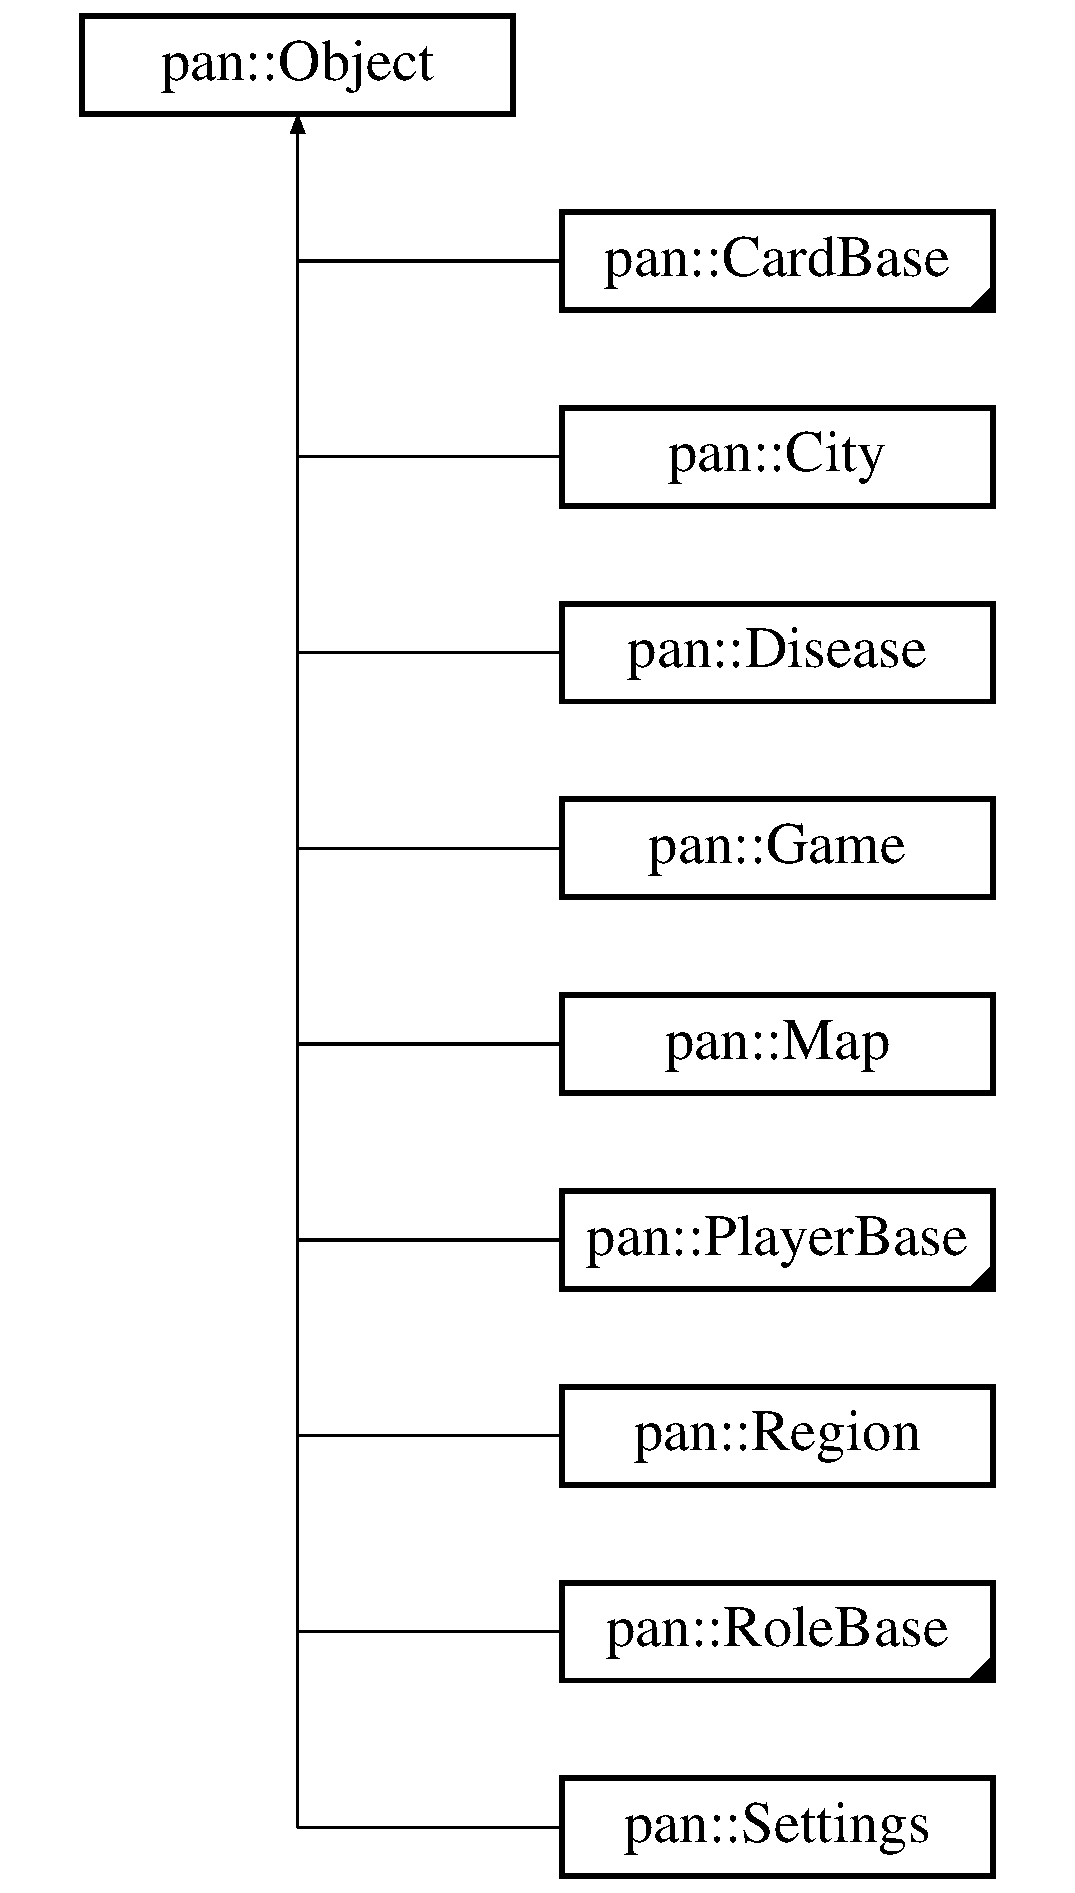
\includegraphics[height=10.000000cm]{classpan_1_1_object}
\end{center}
\end{figure}
\subsection*{Public Member Functions}
\begin{DoxyCompactItemize}
\item 
\hyperlink{classpan_1_1_object_a2ee7680fdf1f046d5f6f4a8bd5529725}{Object} ()
\item 
virtual \hyperlink{classpan_1_1_object_a88ddecef476f026deda410f3b95fe9ca}{$\sim$\+Object} ()
\item 
virtual std\+::string \hyperlink{classpan_1_1_object_a2bb6d3117bb32f5774657c83f118ed8b}{description} () const =0
\item 
{\footnotesize template$<$class Archive $>$ }\\void \hyperlink{classpan_1_1_object_aa69aa8f0aaf6b5b1cd8cd574a00b5b56}{serialize} (Archive \&ar, const unsigned int)
\end{DoxyCompactItemize}
\subsection*{Friends}
\begin{DoxyCompactItemize}
\item 
class \hyperlink{classpan_1_1_object_ac98d07dd8f7b70e16ccb9a01abf56b9c}{boost\+::serialization\+::access}
\end{DoxyCompactItemize}


\subsection{Detailed Description}
Abstract parent class to all entities directly connected with the game state that have to be serialized. 

\subsection{Constructor \& Destructor Documentation}
\mbox{\Hypertarget{classpan_1_1_object_a2ee7680fdf1f046d5f6f4a8bd5529725}\label{classpan_1_1_object_a2ee7680fdf1f046d5f6f4a8bd5529725}} 
\index{pan\+::\+Object@{pan\+::\+Object}!Object@{Object}}
\index{Object@{Object}!pan\+::\+Object@{pan\+::\+Object}}
\subsubsection{\texorpdfstring{Object()}{Object()}}
{\footnotesize\ttfamily pan\+::\+Object\+::\+Object (\begin{DoxyParamCaption}{ }\end{DoxyParamCaption})\hspace{0.3cm}{\ttfamily [inline]}}

\mbox{\Hypertarget{classpan_1_1_object_a88ddecef476f026deda410f3b95fe9ca}\label{classpan_1_1_object_a88ddecef476f026deda410f3b95fe9ca}} 
\index{pan\+::\+Object@{pan\+::\+Object}!````~Object@{$\sim$\+Object}}
\index{````~Object@{$\sim$\+Object}!pan\+::\+Object@{pan\+::\+Object}}
\subsubsection{\texorpdfstring{$\sim$\+Object()}{~Object()}}
{\footnotesize\ttfamily virtual pan\+::\+Object\+::$\sim$\+Object (\begin{DoxyParamCaption}{ }\end{DoxyParamCaption})\hspace{0.3cm}{\ttfamily [inline]}, {\ttfamily [virtual]}}



\subsection{Member Function Documentation}
\mbox{\Hypertarget{classpan_1_1_object_a2bb6d3117bb32f5774657c83f118ed8b}\label{classpan_1_1_object_a2bb6d3117bb32f5774657c83f118ed8b}} 
\index{pan\+::\+Object@{pan\+::\+Object}!description@{description}}
\index{description@{description}!pan\+::\+Object@{pan\+::\+Object}}
\subsubsection{\texorpdfstring{description()}{description()}}
{\footnotesize\ttfamily virtual std\+::string pan\+::\+Object\+::description (\begin{DoxyParamCaption}{ }\end{DoxyParamCaption}) const\hspace{0.3cm}{\ttfamily [pure virtual]}}



Implemented in \hyperlink{classpan_1_1_game_a463480ea3f29b34629059134c416ffa0}{pan\+::\+Game}, \hyperlink{classpan_1_1_settings_ac88db54a696993babc9c495d54fc89c3}{pan\+::\+Settings}, \hyperlink{classpan_1_1_map_a9d08be170f445bbef11ea0d38ba8c531}{pan\+::\+Map}, \hyperlink{classpan_1_1_role_base_a6f4774e52750478d865c4627fc4d4460}{pan\+::\+Role\+Base}, \hyperlink{classpan_1_1_card_impl_3_01_card_type_1_1_event_01_4_aa5c7d2729e0bfb141a0d8487a590a580}{pan\+::\+Card\+Impl$<$ Card\+Type\+::\+Event $>$}, \hyperlink{classpan_1_1_card_base_ad004c502404a958eaf4ecae7e73cc8cf}{pan\+::\+Card\+Base}, \hyperlink{classpan_1_1_player_base_a9b3e10457a0d749d97d91b6461882ac6}{pan\+::\+Player\+Base}, \hyperlink{classpan_1_1_city_a0232df988764b10f50570e335e8237c2}{pan\+::\+City}, \hyperlink{classpan_1_1_disease_a56ea3e8918baf355ad2d1aa253fd9f65}{pan\+::\+Disease}, \hyperlink{classpan_1_1_card_impl_3_01_card_type_1_1_city_01_4_a326c3eaac225bd758f19abb152deffe4}{pan\+::\+Card\+Impl$<$ Card\+Type\+::\+City $>$}, \hyperlink{classpan_1_1_card_impl_3_01_card_type_1_1_infection_01_4_a5e31904120b655ce59633433a4d4c17c}{pan\+::\+Card\+Impl$<$ Card\+Type\+::\+Infection $>$}, and \hyperlink{classpan_1_1_region_abc67a788365510bfad231939713106cb}{pan\+::\+Region}.

\mbox{\Hypertarget{classpan_1_1_object_aa69aa8f0aaf6b5b1cd8cd574a00b5b56}\label{classpan_1_1_object_aa69aa8f0aaf6b5b1cd8cd574a00b5b56}} 
\index{pan\+::\+Object@{pan\+::\+Object}!serialize@{serialize}}
\index{serialize@{serialize}!pan\+::\+Object@{pan\+::\+Object}}
\subsubsection{\texorpdfstring{serialize()}{serialize()}}
{\footnotesize\ttfamily template$<$class Archive $>$ \\
void pan\+::\+Object\+::serialize (\begin{DoxyParamCaption}\item[{Archive \&}]{ar,  }\item[{const unsigned}]{int }\end{DoxyParamCaption})\hspace{0.3cm}{\ttfamily [inline]}}



\subsection{Friends And Related Function Documentation}
\mbox{\Hypertarget{classpan_1_1_object_ac98d07dd8f7b70e16ccb9a01abf56b9c}\label{classpan_1_1_object_ac98d07dd8f7b70e16ccb9a01abf56b9c}} 
\index{pan\+::\+Object@{pan\+::\+Object}!boost\+::serialization\+::access@{boost\+::serialization\+::access}}
\index{boost\+::serialization\+::access@{boost\+::serialization\+::access}!pan\+::\+Object@{pan\+::\+Object}}
\subsubsection{\texorpdfstring{boost\+::serialization\+::access}{boost::serialization::access}}
{\footnotesize\ttfamily friend class boost\+::serialization\+::access\hspace{0.3cm}{\ttfamily [friend]}}



The documentation for this class was generated from the following file\+:\begin{DoxyCompactItemize}
\item 
\hyperlink{_object_8h}{Object.\+h}\end{DoxyCompactItemize}

\hypertarget{classpan_1_1_outbreak}{}\section{pan\+:\+:Outbreak Class Reference}
\label{classpan_1_1_outbreak}\index{pan\+::\+Outbreak@{pan\+::\+Outbreak}}


Encapsulates the parameters of \hyperlink{classpan_1_1_outbreak}{Outbreak} call.  




{\ttfamily \#include $<$Outbreak.\+h$>$}

Inheritance diagram for pan\+:\+:Outbreak\+:\begin{figure}[H]
\begin{center}
\leavevmode
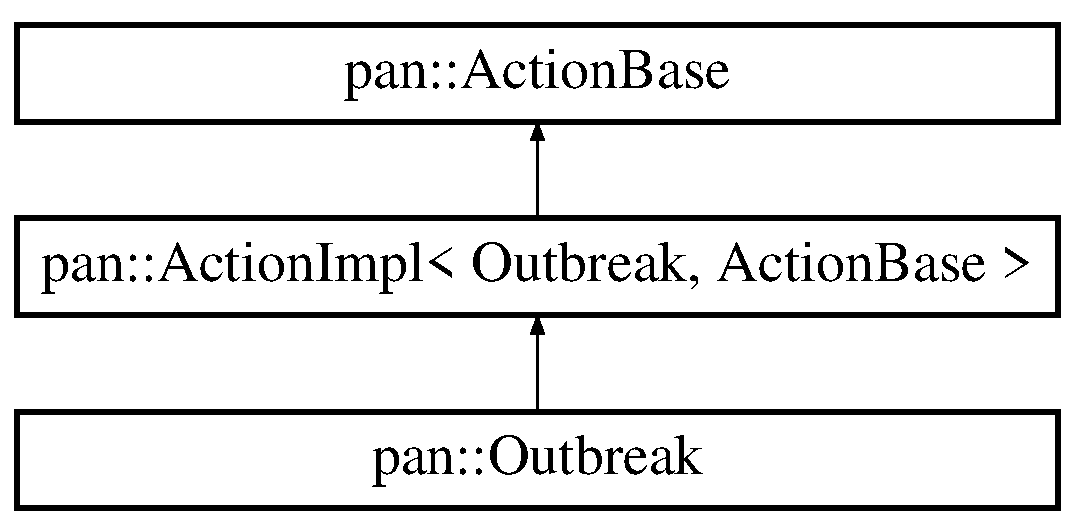
\includegraphics[height=3.000000cm]{classpan_1_1_outbreak}
\end{center}
\end{figure}
\subsection*{Public Member Functions}
\begin{DoxyCompactItemize}
\item 
\hyperlink{classpan_1_1_outbreak_aade590b33f30c7f43f5bb1707234538e}{Outbreak} (const \hyperlink{classpan_1_1_infect}{Infect} \&)
\end{DoxyCompactItemize}
\subsection*{Public Attributes}
\begin{DoxyCompactItemize}
\item 
\hyperlink{classpan_1_1_infect}{Infect} \hyperlink{classpan_1_1_outbreak_a5022e716ec1b51ad1ed9e19a566afdb3}{infection}
\end{DoxyCompactItemize}


\subsection{Detailed Description}
Encapsulates the parameters of \hyperlink{classpan_1_1_outbreak}{Outbreak} call. 

\begin{DoxyAuthor}{Author}
Hrachya Hakobyan 
\end{DoxyAuthor}


\subsection{Constructor \& Destructor Documentation}
\mbox{\Hypertarget{classpan_1_1_outbreak_aade590b33f30c7f43f5bb1707234538e}\label{classpan_1_1_outbreak_aade590b33f30c7f43f5bb1707234538e}} 
\index{pan\+::\+Outbreak@{pan\+::\+Outbreak}!Outbreak@{Outbreak}}
\index{Outbreak@{Outbreak}!pan\+::\+Outbreak@{pan\+::\+Outbreak}}
\subsubsection{\texorpdfstring{Outbreak()}{Outbreak()}}
{\footnotesize\ttfamily pan\+::\+Outbreak\+::\+Outbreak (\begin{DoxyParamCaption}\item[{const \hyperlink{classpan_1_1_infect}{Infect} \&}]{inf }\end{DoxyParamCaption})}



\subsection{Member Data Documentation}
\mbox{\Hypertarget{classpan_1_1_outbreak_a5022e716ec1b51ad1ed9e19a566afdb3}\label{classpan_1_1_outbreak_a5022e716ec1b51ad1ed9e19a566afdb3}} 
\index{pan\+::\+Outbreak@{pan\+::\+Outbreak}!infection@{infection}}
\index{infection@{infection}!pan\+::\+Outbreak@{pan\+::\+Outbreak}}
\subsubsection{\texorpdfstring{infection}{infection}}
{\footnotesize\ttfamily \hyperlink{classpan_1_1_infect}{Infect} pan\+::\+Outbreak\+::infection}



The documentation for this class was generated from the following files\+:\begin{DoxyCompactItemize}
\item 
\hyperlink{_outbreak_8h}{Outbreak.\+h}\item 
\hyperlink{_outbreak_8cpp}{Outbreak.\+cpp}\end{DoxyCompactItemize}

\hypertarget{classpan_1_1_player}{}\section{pan\+:\+:Player$<$ R $>$ Class Template Reference}
\label{classpan_1_1_player}\index{pan\+::\+Player$<$ R $>$@{pan\+::\+Player$<$ R $>$}}


Concrete subclass of \hyperlink{classpan_1_1_player_base}{Player\+Base} The \hyperlink{classpan_1_1_player}{Player} class accepts a template parameter which must be a Roles enum type.  




{\ttfamily \#include $<$Player.\+h$>$}

Inheritance diagram for pan\+:\+:Player$<$ R $>$\+:\begin{figure}[H]
\begin{center}
\leavevmode
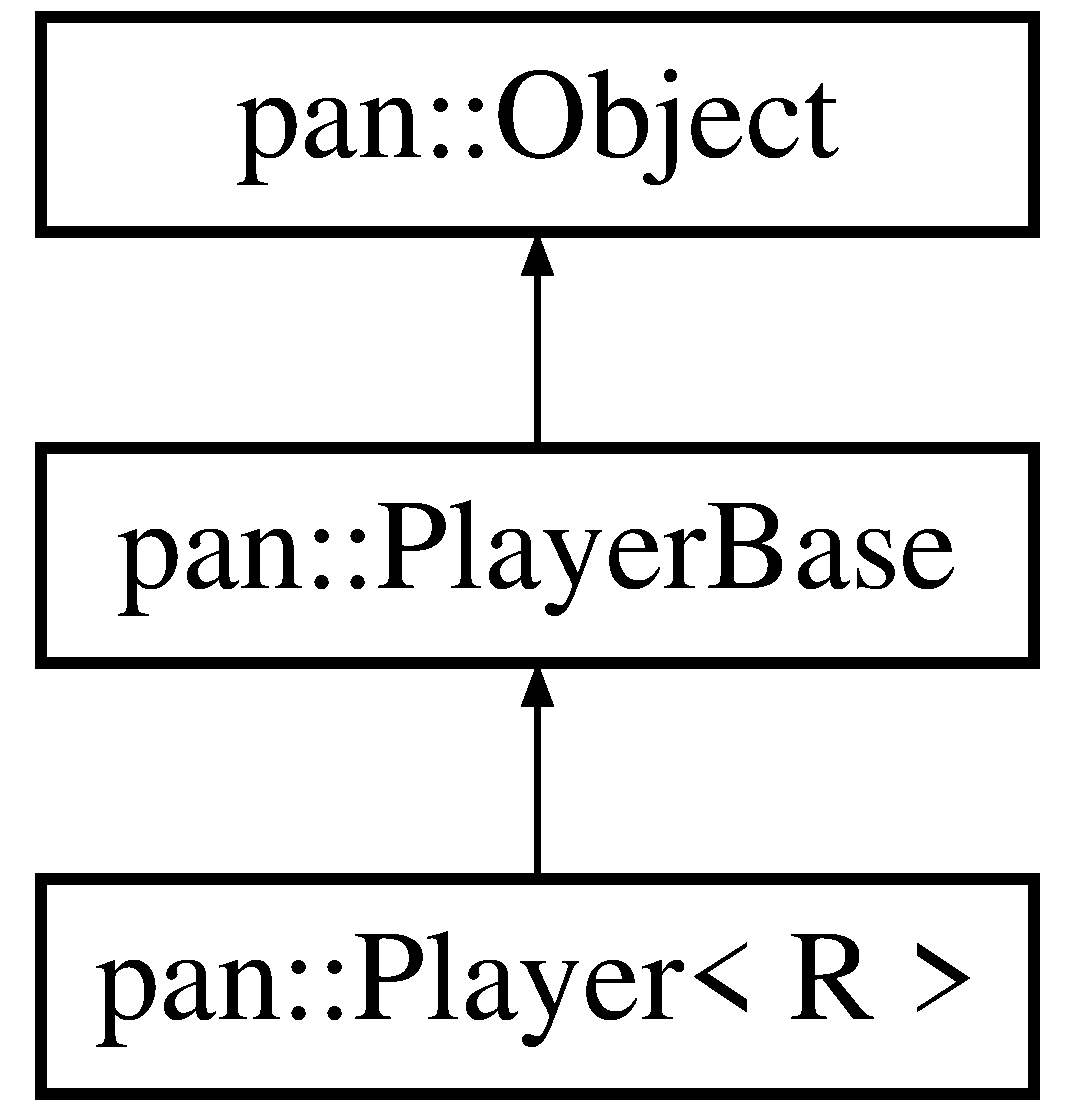
\includegraphics[height=3.000000cm]{classpan_1_1_player}
\end{center}
\end{figure}
\subsection*{Public Member Functions}
\begin{DoxyCompactItemize}
\item 
\hyperlink{classpan_1_1_player_a107eee283242e1a091c19bf801ace02e}{Player} ()
\item 
\hyperlink{classpan_1_1_player_a342d676058285ed15edcb47fc233594b}{Player} (const std\+::string \&\hyperlink{classpan_1_1_player_base_a95bf8887210003d8780dec9d84743a64}{name})
\item 
\hyperlink{classpan_1_1_player_a7571870e341d4413df5e9253ce36534f}{$\sim$\+Player} ()
\item 
{\footnotesize template$<$class Archive $>$ }\\void \hyperlink{classpan_1_1_player_a7aa4f9237095b37b3796f98436bca7bc}{serialize} (Archive \&ar, const unsigned int)
\end{DoxyCompactItemize}
\subsection*{Friends}
\begin{DoxyCompactItemize}
\item 
class \hyperlink{classpan_1_1_player_ac98d07dd8f7b70e16ccb9a01abf56b9c}{boost\+::serialization\+::access}
\end{DoxyCompactItemize}
\subsection*{Additional Inherited Members}


\subsection{Detailed Description}
\subsubsection*{template$<$Roles R$>$\newline
class pan\+::\+Player$<$ R $>$}

Concrete subclass of \hyperlink{classpan_1_1_player_base}{Player\+Base} The \hyperlink{classpan_1_1_player}{Player} class accepts a template parameter which must be a Roles enum type. 

\begin{DoxyAuthor}{Author}
Hrachya Hakobyan 
\end{DoxyAuthor}


\subsection{Constructor \& Destructor Documentation}
\mbox{\Hypertarget{classpan_1_1_player_a107eee283242e1a091c19bf801ace02e}\label{classpan_1_1_player_a107eee283242e1a091c19bf801ace02e}} 
\index{pan\+::\+Player@{pan\+::\+Player}!Player@{Player}}
\index{Player@{Player}!pan\+::\+Player@{pan\+::\+Player}}
\subsubsection{\texorpdfstring{Player()}{Player()}\hspace{0.1cm}{\footnotesize\ttfamily [1/2]}}
{\footnotesize\ttfamily template$<$Roles R$>$ \\
\hyperlink{classpan_1_1_player}{pan\+::\+Player}$<$ R $>$\+::\hyperlink{classpan_1_1_player}{Player} (\begin{DoxyParamCaption}{ }\end{DoxyParamCaption})}

\mbox{\Hypertarget{classpan_1_1_player_a342d676058285ed15edcb47fc233594b}\label{classpan_1_1_player_a342d676058285ed15edcb47fc233594b}} 
\index{pan\+::\+Player@{pan\+::\+Player}!Player@{Player}}
\index{Player@{Player}!pan\+::\+Player@{pan\+::\+Player}}
\subsubsection{\texorpdfstring{Player()}{Player()}\hspace{0.1cm}{\footnotesize\ttfamily [2/2]}}
{\footnotesize\ttfamily template$<$Roles R$>$ \\
\hyperlink{classpan_1_1_player}{pan\+::\+Player}$<$ R $>$\+::\hyperlink{classpan_1_1_player}{Player} (\begin{DoxyParamCaption}\item[{const std\+::string \&}]{name }\end{DoxyParamCaption})}

\mbox{\Hypertarget{classpan_1_1_player_a7571870e341d4413df5e9253ce36534f}\label{classpan_1_1_player_a7571870e341d4413df5e9253ce36534f}} 
\index{pan\+::\+Player@{pan\+::\+Player}!````~Player@{$\sim$\+Player}}
\index{````~Player@{$\sim$\+Player}!pan\+::\+Player@{pan\+::\+Player}}
\subsubsection{\texorpdfstring{$\sim$\+Player()}{~Player()}}
{\footnotesize\ttfamily template$<$Roles R$>$ \\
\hyperlink{classpan_1_1_player}{pan\+::\+Player}$<$ R $>$\+::$\sim$\hyperlink{classpan_1_1_player}{Player} (\begin{DoxyParamCaption}{ }\end{DoxyParamCaption})}



\subsection{Member Function Documentation}
\mbox{\Hypertarget{classpan_1_1_player_a7aa4f9237095b37b3796f98436bca7bc}\label{classpan_1_1_player_a7aa4f9237095b37b3796f98436bca7bc}} 
\index{pan\+::\+Player@{pan\+::\+Player}!serialize@{serialize}}
\index{serialize@{serialize}!pan\+::\+Player@{pan\+::\+Player}}
\subsubsection{\texorpdfstring{serialize()}{serialize()}}
{\footnotesize\ttfamily template$<$Roles R$>$ \\
template$<$class Archive $>$ \\
void \hyperlink{classpan_1_1_player}{pan\+::\+Player}$<$ R $>$\+::serialize (\begin{DoxyParamCaption}\item[{Archive \&}]{ar,  }\item[{const unsigned}]{int }\end{DoxyParamCaption})\hspace{0.3cm}{\ttfamily [inline]}}



\subsection{Friends And Related Function Documentation}
\mbox{\Hypertarget{classpan_1_1_player_ac98d07dd8f7b70e16ccb9a01abf56b9c}\label{classpan_1_1_player_ac98d07dd8f7b70e16ccb9a01abf56b9c}} 
\index{pan\+::\+Player@{pan\+::\+Player}!boost\+::serialization\+::access@{boost\+::serialization\+::access}}
\index{boost\+::serialization\+::access@{boost\+::serialization\+::access}!pan\+::\+Player@{pan\+::\+Player}}
\subsubsection{\texorpdfstring{boost\+::serialization\+::access}{boost::serialization::access}}
{\footnotesize\ttfamily template$<$Roles R$>$ \\
friend class boost\+::serialization\+::access\hspace{0.3cm}{\ttfamily [friend]}}



The documentation for this class was generated from the following file\+:\begin{DoxyCompactItemize}
\item 
\hyperlink{_player_8h}{Player.\+h}\end{DoxyCompactItemize}

\hypertarget{classpan_1_1_player_base}{}\section{pan\+:\+:Player\+Base Class Reference}
\label{classpan_1_1_player_base}\index{pan\+::\+Player\+Base@{pan\+::\+Player\+Base}}


Base class for player objects.  




{\ttfamily \#include $<$Player\+Base.\+h$>$}

Inheritance diagram for pan\+:\+:Player\+Base\+:\begin{figure}[H]
\begin{center}
\leavevmode
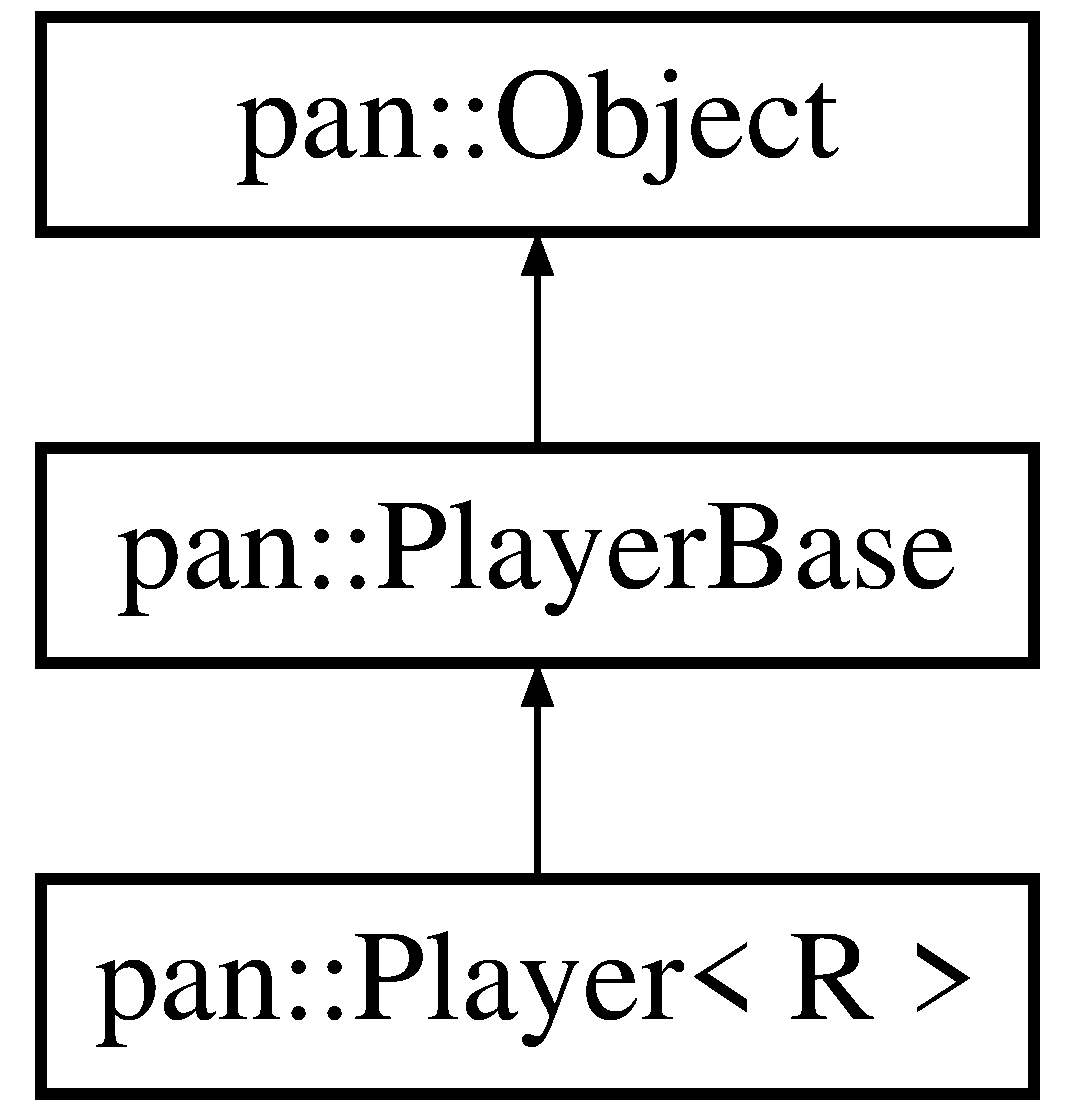
\includegraphics[height=3.000000cm]{classpan_1_1_player_base}
\end{center}
\end{figure}
\subsection*{Public Member Functions}
\begin{DoxyCompactItemize}
\item 
virtual \hyperlink{classpan_1_1_player_base_ab2f4c99f8580f417a2f79534048ebc22}{$\sim$\+Player\+Base} ()
\item 
bool \hyperlink{classpan_1_1_player_base_a6af9e045f23aae67188ec154202d8048}{operator==} (const \hyperlink{classpan_1_1_player_base}{Player\+Base} \&) const
\item 
bool \hyperlink{classpan_1_1_player_base_a95f1b22c858ea2ceefbcff6a52c7312a}{operator!=} (const \hyperlink{classpan_1_1_player_base}{Player\+Base} \&) const
\item 
const std\+::string \& \hyperlink{classpan_1_1_player_base_a427d73fde6596033fbe0ebd511d1e7c1}{get\+Name} () const
\item 
void \hyperlink{classpan_1_1_player_base_a7c8cf80013d7ffa5139a33e3a5d8d395}{set\+Name} (const std\+::string \&\hyperlink{classpan_1_1_player_base_a95bf8887210003d8780dec9d84743a64}{name})
\item 
\hyperlink{namespacepan_afaed28aa6603153dcc062a028602d697}{City\+Index} \hyperlink{classpan_1_1_player_base_aa4bc65b9e86fa2b506f5191be751cfea}{get\+Location} () const
\item 
void \hyperlink{classpan_1_1_player_base_ad124348adae23b1d6b85fe1359b7c752}{set\+Location} (\hyperlink{namespacepan_afaed28aa6603153dcc062a028602d697}{City\+Index})
\item 
\hyperlink{classpan_1_1detail_1_1_deck}{detail\+::\+Deck}$<$ std\+::shared\+\_\+ptr$<$ \hyperlink{classpan_1_1_card_base}{Card\+Base} $>$ $>$ \& \hyperlink{classpan_1_1_player_base_ada4d9050732037e7436cb78244ec177b}{get\+Cards} ()
\item 
const \hyperlink{classpan_1_1detail_1_1_deck}{detail\+::\+Deck}$<$ std\+::shared\+\_\+ptr$<$ \hyperlink{classpan_1_1_card_base}{Card\+Base} $>$ $>$ \& \hyperlink{classpan_1_1_player_base_a8c23e4d5910f85c0e942f3b0819743af}{get\+Cards} () const
\item 
void \hyperlink{classpan_1_1_player_base_a94e33fc8f12381165320363b2886b7f6}{set\+Cards} (const \hyperlink{classpan_1_1detail_1_1_deck}{detail\+::\+Deck}$<$ std\+::shared\+\_\+ptr$<$ \hyperlink{classpan_1_1_card_base}{Card\+Base} $>$$>$ \&)
\item 
std\+::string \hyperlink{classpan_1_1_player_base_a9b3e10457a0d749d97d91b6461882ac6}{description} () const
\item 
{\footnotesize template$<$class Archive $>$ }\\void \hyperlink{classpan_1_1_player_base_a8b884015c320a552d9021e507285d392}{serialize} (Archive \&ar, const unsigned int)
\end{DoxyCompactItemize}
\subsection*{Public Attributes}
\begin{DoxyCompactItemize}
\item 
const \hyperlink{classpan_1_1_role_base}{Role\+Base} \hyperlink{classpan_1_1_player_base_a63c1e92022a4eb34dc3a59d516ee6cea}{role}
\item 
const \hyperlink{classpan_1_1_reference_card}{Reference\+Card} \hyperlink{classpan_1_1_player_base_ae222fd3f8e044135bcc5d52fdd786804}{reference\+Card}
\end{DoxyCompactItemize}
\subsection*{Protected Member Functions}
\begin{DoxyCompactItemize}
\item 
\hyperlink{classpan_1_1_player_base_a3299b54cef6713e3d81313fd9a8f501d}{Player\+Base} (const \hyperlink{classpan_1_1_role_base}{Role\+Base} \&\hyperlink{classpan_1_1_player_base_a63c1e92022a4eb34dc3a59d516ee6cea}{role})
\item 
\hyperlink{classpan_1_1_player_base_af93832f2887f4e7c4242cb28ca881b1a}{Player\+Base} (const \hyperlink{classpan_1_1_role_base}{Role\+Base} \&\hyperlink{classpan_1_1_player_base_a63c1e92022a4eb34dc3a59d516ee6cea}{role}, const std\+::string \&\hyperlink{classpan_1_1_player_base_a95bf8887210003d8780dec9d84743a64}{name})
\end{DoxyCompactItemize}
\subsection*{Protected Attributes}
\begin{DoxyCompactItemize}
\item 
\hyperlink{classpan_1_1detail_1_1_deck}{detail\+::\+Deck}$<$ std\+::shared\+\_\+ptr$<$ \hyperlink{classpan_1_1_card_base}{Card\+Base} $>$ $>$ \hyperlink{classpan_1_1_player_base_a0f4e9109bf26267371442b2d5da75c49}{cards}
\item 
std\+::string \hyperlink{classpan_1_1_player_base_a95bf8887210003d8780dec9d84743a64}{name}
\item 
\hyperlink{namespacepan_afaed28aa6603153dcc062a028602d697}{City\+Index} \hyperlink{classpan_1_1_player_base_ad5b88869afb5740cf34f226fe36c5f27}{location}
\end{DoxyCompactItemize}
\subsection*{Friends}
\begin{DoxyCompactItemize}
\item 
class \hyperlink{classpan_1_1_player_base_ac98d07dd8f7b70e16ccb9a01abf56b9c}{boost\+::serialization\+::access}
\end{DoxyCompactItemize}


\subsection{Detailed Description}
Base class for player objects. 

\begin{DoxyAuthor}{Author}
Hrachya Hakobyan 
\end{DoxyAuthor}


\subsection{Constructor \& Destructor Documentation}
\mbox{\Hypertarget{classpan_1_1_player_base_ab2f4c99f8580f417a2f79534048ebc22}\label{classpan_1_1_player_base_ab2f4c99f8580f417a2f79534048ebc22}} 
\index{pan\+::\+Player\+Base@{pan\+::\+Player\+Base}!````~Player\+Base@{$\sim$\+Player\+Base}}
\index{````~Player\+Base@{$\sim$\+Player\+Base}!pan\+::\+Player\+Base@{pan\+::\+Player\+Base}}
\subsubsection{\texorpdfstring{$\sim$\+Player\+Base()}{~PlayerBase()}}
{\footnotesize\ttfamily pan\+::\+Player\+Base\+::$\sim$\+Player\+Base (\begin{DoxyParamCaption}{ }\end{DoxyParamCaption})\hspace{0.3cm}{\ttfamily [virtual]}}

\mbox{\Hypertarget{classpan_1_1_player_base_a3299b54cef6713e3d81313fd9a8f501d}\label{classpan_1_1_player_base_a3299b54cef6713e3d81313fd9a8f501d}} 
\index{pan\+::\+Player\+Base@{pan\+::\+Player\+Base}!Player\+Base@{Player\+Base}}
\index{Player\+Base@{Player\+Base}!pan\+::\+Player\+Base@{pan\+::\+Player\+Base}}
\subsubsection{\texorpdfstring{Player\+Base()}{PlayerBase()}\hspace{0.1cm}{\footnotesize\ttfamily [1/2]}}
{\footnotesize\ttfamily pan\+::\+Player\+Base\+::\+Player\+Base (\begin{DoxyParamCaption}\item[{const \hyperlink{classpan_1_1_role_base}{Role\+Base} \&}]{role }\end{DoxyParamCaption})\hspace{0.3cm}{\ttfamily [protected]}}

\mbox{\Hypertarget{classpan_1_1_player_base_af93832f2887f4e7c4242cb28ca881b1a}\label{classpan_1_1_player_base_af93832f2887f4e7c4242cb28ca881b1a}} 
\index{pan\+::\+Player\+Base@{pan\+::\+Player\+Base}!Player\+Base@{Player\+Base}}
\index{Player\+Base@{Player\+Base}!pan\+::\+Player\+Base@{pan\+::\+Player\+Base}}
\subsubsection{\texorpdfstring{Player\+Base()}{PlayerBase()}\hspace{0.1cm}{\footnotesize\ttfamily [2/2]}}
{\footnotesize\ttfamily pan\+::\+Player\+Base\+::\+Player\+Base (\begin{DoxyParamCaption}\item[{const \hyperlink{classpan_1_1_role_base}{Role\+Base} \&}]{role,  }\item[{const std\+::string \&}]{name }\end{DoxyParamCaption})\hspace{0.3cm}{\ttfamily [protected]}}



\subsection{Member Function Documentation}
\mbox{\Hypertarget{classpan_1_1_player_base_a9b3e10457a0d749d97d91b6461882ac6}\label{classpan_1_1_player_base_a9b3e10457a0d749d97d91b6461882ac6}} 
\index{pan\+::\+Player\+Base@{pan\+::\+Player\+Base}!description@{description}}
\index{description@{description}!pan\+::\+Player\+Base@{pan\+::\+Player\+Base}}
\subsubsection{\texorpdfstring{description()}{description()}}
{\footnotesize\ttfamily std\+::string pan\+::\+Player\+Base\+::description (\begin{DoxyParamCaption}{ }\end{DoxyParamCaption}) const\hspace{0.3cm}{\ttfamily [virtual]}}



Implements \hyperlink{classpan_1_1_object_a2bb6d3117bb32f5774657c83f118ed8b}{pan\+::\+Object}.

\mbox{\Hypertarget{classpan_1_1_player_base_ada4d9050732037e7436cb78244ec177b}\label{classpan_1_1_player_base_ada4d9050732037e7436cb78244ec177b}} 
\index{pan\+::\+Player\+Base@{pan\+::\+Player\+Base}!get\+Cards@{get\+Cards}}
\index{get\+Cards@{get\+Cards}!pan\+::\+Player\+Base@{pan\+::\+Player\+Base}}
\subsubsection{\texorpdfstring{get\+Cards()}{getCards()}\hspace{0.1cm}{\footnotesize\ttfamily [1/2]}}
{\footnotesize\ttfamily \hyperlink{classpan_1_1detail_1_1_deck}{detail\+::\+Deck}$<$ std\+::shared\+\_\+ptr$<$ \hyperlink{classpan_1_1_card_base}{Card\+Base} $>$ $>$ \& pan\+::\+Player\+Base\+::get\+Cards (\begin{DoxyParamCaption}{ }\end{DoxyParamCaption})\hspace{0.3cm}{\ttfamily [inline]}}

\mbox{\Hypertarget{classpan_1_1_player_base_a8c23e4d5910f85c0e942f3b0819743af}\label{classpan_1_1_player_base_a8c23e4d5910f85c0e942f3b0819743af}} 
\index{pan\+::\+Player\+Base@{pan\+::\+Player\+Base}!get\+Cards@{get\+Cards}}
\index{get\+Cards@{get\+Cards}!pan\+::\+Player\+Base@{pan\+::\+Player\+Base}}
\subsubsection{\texorpdfstring{get\+Cards()}{getCards()}\hspace{0.1cm}{\footnotesize\ttfamily [2/2]}}
{\footnotesize\ttfamily const \hyperlink{classpan_1_1detail_1_1_deck}{detail\+::\+Deck}$<$ std\+::shared\+\_\+ptr$<$ \hyperlink{classpan_1_1_card_base}{Card\+Base} $>$ $>$ \& pan\+::\+Player\+Base\+::get\+Cards (\begin{DoxyParamCaption}{ }\end{DoxyParamCaption}) const\hspace{0.3cm}{\ttfamily [inline]}}

\mbox{\Hypertarget{classpan_1_1_player_base_aa4bc65b9e86fa2b506f5191be751cfea}\label{classpan_1_1_player_base_aa4bc65b9e86fa2b506f5191be751cfea}} 
\index{pan\+::\+Player\+Base@{pan\+::\+Player\+Base}!get\+Location@{get\+Location}}
\index{get\+Location@{get\+Location}!pan\+::\+Player\+Base@{pan\+::\+Player\+Base}}
\subsubsection{\texorpdfstring{get\+Location()}{getLocation()}}
{\footnotesize\ttfamily \hyperlink{namespacepan_afaed28aa6603153dcc062a028602d697}{City\+Index} pan\+::\+Player\+Base\+::get\+Location (\begin{DoxyParamCaption}{ }\end{DoxyParamCaption}) const\hspace{0.3cm}{\ttfamily [inline]}}

\mbox{\Hypertarget{classpan_1_1_player_base_a427d73fde6596033fbe0ebd511d1e7c1}\label{classpan_1_1_player_base_a427d73fde6596033fbe0ebd511d1e7c1}} 
\index{pan\+::\+Player\+Base@{pan\+::\+Player\+Base}!get\+Name@{get\+Name}}
\index{get\+Name@{get\+Name}!pan\+::\+Player\+Base@{pan\+::\+Player\+Base}}
\subsubsection{\texorpdfstring{get\+Name()}{getName()}}
{\footnotesize\ttfamily const std\+::string \& pan\+::\+Player\+Base\+::get\+Name (\begin{DoxyParamCaption}{ }\end{DoxyParamCaption}) const\hspace{0.3cm}{\ttfamily [inline]}}

\mbox{\Hypertarget{classpan_1_1_player_base_a95f1b22c858ea2ceefbcff6a52c7312a}\label{classpan_1_1_player_base_a95f1b22c858ea2ceefbcff6a52c7312a}} 
\index{pan\+::\+Player\+Base@{pan\+::\+Player\+Base}!operator"!=@{operator"!=}}
\index{operator"!=@{operator"!=}!pan\+::\+Player\+Base@{pan\+::\+Player\+Base}}
\subsubsection{\texorpdfstring{operator"!=()}{operator!=()}}
{\footnotesize\ttfamily bool pan\+::\+Player\+Base\+::operator!= (\begin{DoxyParamCaption}\item[{const \hyperlink{classpan_1_1_player_base}{Player\+Base} \&}]{o }\end{DoxyParamCaption}) const\hspace{0.3cm}{\ttfamily [inline]}}

\mbox{\Hypertarget{classpan_1_1_player_base_a6af9e045f23aae67188ec154202d8048}\label{classpan_1_1_player_base_a6af9e045f23aae67188ec154202d8048}} 
\index{pan\+::\+Player\+Base@{pan\+::\+Player\+Base}!operator==@{operator==}}
\index{operator==@{operator==}!pan\+::\+Player\+Base@{pan\+::\+Player\+Base}}
\subsubsection{\texorpdfstring{operator==()}{operator==()}}
{\footnotesize\ttfamily bool pan\+::\+Player\+Base\+::operator== (\begin{DoxyParamCaption}\item[{const \hyperlink{classpan_1_1_player_base}{Player\+Base} \&}]{o }\end{DoxyParamCaption}) const}

\mbox{\Hypertarget{classpan_1_1_player_base_a8b884015c320a552d9021e507285d392}\label{classpan_1_1_player_base_a8b884015c320a552d9021e507285d392}} 
\index{pan\+::\+Player\+Base@{pan\+::\+Player\+Base}!serialize@{serialize}}
\index{serialize@{serialize}!pan\+::\+Player\+Base@{pan\+::\+Player\+Base}}
\subsubsection{\texorpdfstring{serialize()}{serialize()}}
{\footnotesize\ttfamily template$<$class Archive $>$ \\
void pan\+::\+Player\+Base\+::serialize (\begin{DoxyParamCaption}\item[{Archive \&}]{ar,  }\item[{const unsigned}]{int }\end{DoxyParamCaption})\hspace{0.3cm}{\ttfamily [inline]}}

\mbox{\Hypertarget{classpan_1_1_player_base_a94e33fc8f12381165320363b2886b7f6}\label{classpan_1_1_player_base_a94e33fc8f12381165320363b2886b7f6}} 
\index{pan\+::\+Player\+Base@{pan\+::\+Player\+Base}!set\+Cards@{set\+Cards}}
\index{set\+Cards@{set\+Cards}!pan\+::\+Player\+Base@{pan\+::\+Player\+Base}}
\subsubsection{\texorpdfstring{set\+Cards()}{setCards()}}
{\footnotesize\ttfamily void pan\+::\+Player\+Base\+::set\+Cards (\begin{DoxyParamCaption}\item[{const \hyperlink{classpan_1_1detail_1_1_deck}{detail\+::\+Deck}$<$ std\+::shared\+\_\+ptr$<$ \hyperlink{classpan_1_1_card_base}{Card\+Base} $>$$>$ \&}]{cards }\end{DoxyParamCaption})\hspace{0.3cm}{\ttfamily [inline]}}

\mbox{\Hypertarget{classpan_1_1_player_base_ad124348adae23b1d6b85fe1359b7c752}\label{classpan_1_1_player_base_ad124348adae23b1d6b85fe1359b7c752}} 
\index{pan\+::\+Player\+Base@{pan\+::\+Player\+Base}!set\+Location@{set\+Location}}
\index{set\+Location@{set\+Location}!pan\+::\+Player\+Base@{pan\+::\+Player\+Base}}
\subsubsection{\texorpdfstring{set\+Location()}{setLocation()}}
{\footnotesize\ttfamily void pan\+::\+Player\+Base\+::set\+Location (\begin{DoxyParamCaption}\item[{\hyperlink{namespacepan_afaed28aa6603153dcc062a028602d697}{City\+Index}}]{loc }\end{DoxyParamCaption})\hspace{0.3cm}{\ttfamily [inline]}}

\mbox{\Hypertarget{classpan_1_1_player_base_a7c8cf80013d7ffa5139a33e3a5d8d395}\label{classpan_1_1_player_base_a7c8cf80013d7ffa5139a33e3a5d8d395}} 
\index{pan\+::\+Player\+Base@{pan\+::\+Player\+Base}!set\+Name@{set\+Name}}
\index{set\+Name@{set\+Name}!pan\+::\+Player\+Base@{pan\+::\+Player\+Base}}
\subsubsection{\texorpdfstring{set\+Name()}{setName()}}
{\footnotesize\ttfamily void pan\+::\+Player\+Base\+::set\+Name (\begin{DoxyParamCaption}\item[{const std\+::string \&}]{name }\end{DoxyParamCaption})\hspace{0.3cm}{\ttfamily [inline]}}



\subsection{Friends And Related Function Documentation}
\mbox{\Hypertarget{classpan_1_1_player_base_ac98d07dd8f7b70e16ccb9a01abf56b9c}\label{classpan_1_1_player_base_ac98d07dd8f7b70e16ccb9a01abf56b9c}} 
\index{pan\+::\+Player\+Base@{pan\+::\+Player\+Base}!boost\+::serialization\+::access@{boost\+::serialization\+::access}}
\index{boost\+::serialization\+::access@{boost\+::serialization\+::access}!pan\+::\+Player\+Base@{pan\+::\+Player\+Base}}
\subsubsection{\texorpdfstring{boost\+::serialization\+::access}{boost::serialization::access}}
{\footnotesize\ttfamily friend class boost\+::serialization\+::access\hspace{0.3cm}{\ttfamily [friend]}}



\subsection{Member Data Documentation}
\mbox{\Hypertarget{classpan_1_1_player_base_a0f4e9109bf26267371442b2d5da75c49}\label{classpan_1_1_player_base_a0f4e9109bf26267371442b2d5da75c49}} 
\index{pan\+::\+Player\+Base@{pan\+::\+Player\+Base}!cards@{cards}}
\index{cards@{cards}!pan\+::\+Player\+Base@{pan\+::\+Player\+Base}}
\subsubsection{\texorpdfstring{cards}{cards}}
{\footnotesize\ttfamily \hyperlink{classpan_1_1detail_1_1_deck}{detail\+::\+Deck}$<$std\+::shared\+\_\+ptr$<$\hyperlink{classpan_1_1_card_base}{Card\+Base}$>$ $>$ pan\+::\+Player\+Base\+::cards\hspace{0.3cm}{\ttfamily [protected]}}

\mbox{\Hypertarget{classpan_1_1_player_base_ad5b88869afb5740cf34f226fe36c5f27}\label{classpan_1_1_player_base_ad5b88869afb5740cf34f226fe36c5f27}} 
\index{pan\+::\+Player\+Base@{pan\+::\+Player\+Base}!location@{location}}
\index{location@{location}!pan\+::\+Player\+Base@{pan\+::\+Player\+Base}}
\subsubsection{\texorpdfstring{location}{location}}
{\footnotesize\ttfamily \hyperlink{namespacepan_afaed28aa6603153dcc062a028602d697}{City\+Index} pan\+::\+Player\+Base\+::location\hspace{0.3cm}{\ttfamily [protected]}}

\mbox{\Hypertarget{classpan_1_1_player_base_a95bf8887210003d8780dec9d84743a64}\label{classpan_1_1_player_base_a95bf8887210003d8780dec9d84743a64}} 
\index{pan\+::\+Player\+Base@{pan\+::\+Player\+Base}!name@{name}}
\index{name@{name}!pan\+::\+Player\+Base@{pan\+::\+Player\+Base}}
\subsubsection{\texorpdfstring{name}{name}}
{\footnotesize\ttfamily std\+::string pan\+::\+Player\+Base\+::name\hspace{0.3cm}{\ttfamily [protected]}}

\mbox{\Hypertarget{classpan_1_1_player_base_ae222fd3f8e044135bcc5d52fdd786804}\label{classpan_1_1_player_base_ae222fd3f8e044135bcc5d52fdd786804}} 
\index{pan\+::\+Player\+Base@{pan\+::\+Player\+Base}!reference\+Card@{reference\+Card}}
\index{reference\+Card@{reference\+Card}!pan\+::\+Player\+Base@{pan\+::\+Player\+Base}}
\subsubsection{\texorpdfstring{reference\+Card}{referenceCard}}
{\footnotesize\ttfamily const \hyperlink{classpan_1_1_reference_card}{Reference\+Card} pan\+::\+Player\+Base\+::reference\+Card}

\mbox{\Hypertarget{classpan_1_1_player_base_a63c1e92022a4eb34dc3a59d516ee6cea}\label{classpan_1_1_player_base_a63c1e92022a4eb34dc3a59d516ee6cea}} 
\index{pan\+::\+Player\+Base@{pan\+::\+Player\+Base}!role@{role}}
\index{role@{role}!pan\+::\+Player\+Base@{pan\+::\+Player\+Base}}
\subsubsection{\texorpdfstring{role}{role}}
{\footnotesize\ttfamily const \hyperlink{classpan_1_1_role_base}{Role\+Base} pan\+::\+Player\+Base\+::role}



The documentation for this class was generated from the following files\+:\begin{DoxyCompactItemize}
\item 
\hyperlink{_player_base_8h}{Player\+Base.\+h}\item 
\hyperlink{_player_base_8cpp}{Player\+Base.\+cpp}\end{DoxyCompactItemize}

\hypertarget{structpan_1_1_player_data}{}\section{pan\+:\+:Player\+Data Struct Reference}
\label{structpan_1_1_player_data}\index{pan\+::\+Player\+Data@{pan\+::\+Player\+Data}}


container for player related data  




{\ttfamily \#include $<$Data.\+h$>$}

\subsection*{Public Member Functions}
\begin{DoxyCompactItemize}
\item 
\hyperlink{structpan_1_1_player_data_a7bd4ebf550c2dd24d62fe443a2494a7b}{Player\+Data} ()
\item 
\hyperlink{structpan_1_1_player_data_ac73829f7cb3159a7b4c73c5e1692c8dd}{Player\+Data} (const \hyperlink{structpan_1_1_player_data}{Player\+Data} \&)
\item 
\hyperlink{structpan_1_1_player_data}{Player\+Data} \& \hyperlink{structpan_1_1_player_data_af777062227dfc1e659b35dd3fd630028}{operator=} (const \hyperlink{structpan_1_1_player_data}{Player\+Data} \&)
\item 
\hyperlink{structpan_1_1_player_data_af4aeaccb9684a634521e4e9cf140e769}{Player\+Data} (\hyperlink{structpan_1_1_player_data}{Player\+Data} \&\&)
\item 
\hyperlink{structpan_1_1_player_data}{Player\+Data} \& \hyperlink{structpan_1_1_player_data_aa4adc4de5012f149b3bc5ec52db85478}{operator=} (\hyperlink{structpan_1_1_player_data}{Player\+Data} \&\&)
\item 
\hyperlink{structpan_1_1_player_data_ae8c8ca3b7b8a98f238748a6031a08724}{$\sim$\+Player\+Data} ()
\item 
bool \hyperlink{structpan_1_1_player_data_af931fa445725740d81b14edbff520f00}{operator==} (const \hyperlink{structpan_1_1_player_data}{Player\+Data} \&) const
\item 
bool \hyperlink{structpan_1_1_player_data_a6bc35b4e97c2d0f26f03f32e04fcf3f0}{operator!=} (const \hyperlink{structpan_1_1_player_data}{Player\+Data} \&) const
\item 
std\+::string \hyperlink{structpan_1_1_player_data_a6b3e95835968243be8b690eacb732d5b}{description} () const
\end{DoxyCompactItemize}
\subsection*{Public Attributes}
\begin{DoxyCompactItemize}
\item 
\hyperlink{namespacepan_a0cdabf874fbf1bb3a1f0152d108c2909}{Player\+Index} \hyperlink{structpan_1_1_player_data_a5e25e3064088436cb55df4d1fe256cb0}{turn}
\item 
\hyperlink{namespacepan_a5c203ea0600f2bca14baf8f38e5bac5d}{Player\+Stage} \hyperlink{structpan_1_1_player_data_a8f06369e6df4f62a3d5be54cace7aa17}{stage}
\item 
unsigned int \hyperlink{structpan_1_1_player_data_a088b5b37693cc53f7be4c3f2860c6648}{action\+Counter}
\item 
std\+::vector$<$ std\+::shared\+\_\+ptr$<$ \hyperlink{classpan_1_1_player_base}{Player\+Base} $>$ $>$ \hyperlink{structpan_1_1_player_data_a44a9f5f24c1020e2c186205e08c184c5}{players}
\item 
std\+::vector$<$ bool $>$ \hyperlink{structpan_1_1_player_data_aa79e564016ca865b17e4bf1b241fc827}{occupied\+Roles}
\end{DoxyCompactItemize}


\subsection{Detailed Description}
container for player related data 

\begin{DoxyAuthor}{Author}
Hrachya Hakobyan 
\end{DoxyAuthor}


\subsection{Constructor \& Destructor Documentation}
\mbox{\Hypertarget{structpan_1_1_player_data_a7bd4ebf550c2dd24d62fe443a2494a7b}\label{structpan_1_1_player_data_a7bd4ebf550c2dd24d62fe443a2494a7b}} 
\index{pan\+::\+Player\+Data@{pan\+::\+Player\+Data}!Player\+Data@{Player\+Data}}
\index{Player\+Data@{Player\+Data}!pan\+::\+Player\+Data@{pan\+::\+Player\+Data}}
\subsubsection{\texorpdfstring{Player\+Data()}{PlayerData()}\hspace{0.1cm}{\footnotesize\ttfamily [1/3]}}
{\footnotesize\ttfamily pan\+::\+Player\+Data\+::\+Player\+Data (\begin{DoxyParamCaption}{ }\end{DoxyParamCaption})}

\mbox{\Hypertarget{structpan_1_1_player_data_ac73829f7cb3159a7b4c73c5e1692c8dd}\label{structpan_1_1_player_data_ac73829f7cb3159a7b4c73c5e1692c8dd}} 
\index{pan\+::\+Player\+Data@{pan\+::\+Player\+Data}!Player\+Data@{Player\+Data}}
\index{Player\+Data@{Player\+Data}!pan\+::\+Player\+Data@{pan\+::\+Player\+Data}}
\subsubsection{\texorpdfstring{Player\+Data()}{PlayerData()}\hspace{0.1cm}{\footnotesize\ttfamily [2/3]}}
{\footnotesize\ttfamily pan\+::\+Player\+Data\+::\+Player\+Data (\begin{DoxyParamCaption}\item[{const \hyperlink{structpan_1_1_player_data}{Player\+Data} \&}]{o }\end{DoxyParamCaption})}

\mbox{\Hypertarget{structpan_1_1_player_data_af4aeaccb9684a634521e4e9cf140e769}\label{structpan_1_1_player_data_af4aeaccb9684a634521e4e9cf140e769}} 
\index{pan\+::\+Player\+Data@{pan\+::\+Player\+Data}!Player\+Data@{Player\+Data}}
\index{Player\+Data@{Player\+Data}!pan\+::\+Player\+Data@{pan\+::\+Player\+Data}}
\subsubsection{\texorpdfstring{Player\+Data()}{PlayerData()}\hspace{0.1cm}{\footnotesize\ttfamily [3/3]}}
{\footnotesize\ttfamily pan\+::\+Player\+Data\+::\+Player\+Data (\begin{DoxyParamCaption}\item[{\hyperlink{structpan_1_1_player_data}{Player\+Data} \&\&}]{o }\end{DoxyParamCaption})}

\mbox{\Hypertarget{structpan_1_1_player_data_ae8c8ca3b7b8a98f238748a6031a08724}\label{structpan_1_1_player_data_ae8c8ca3b7b8a98f238748a6031a08724}} 
\index{pan\+::\+Player\+Data@{pan\+::\+Player\+Data}!````~Player\+Data@{$\sim$\+Player\+Data}}
\index{````~Player\+Data@{$\sim$\+Player\+Data}!pan\+::\+Player\+Data@{pan\+::\+Player\+Data}}
\subsubsection{\texorpdfstring{$\sim$\+Player\+Data()}{~PlayerData()}}
{\footnotesize\ttfamily pan\+::\+Player\+Data\+::$\sim$\+Player\+Data (\begin{DoxyParamCaption}{ }\end{DoxyParamCaption})}



\subsection{Member Function Documentation}
\mbox{\Hypertarget{structpan_1_1_player_data_a6b3e95835968243be8b690eacb732d5b}\label{structpan_1_1_player_data_a6b3e95835968243be8b690eacb732d5b}} 
\index{pan\+::\+Player\+Data@{pan\+::\+Player\+Data}!description@{description}}
\index{description@{description}!pan\+::\+Player\+Data@{pan\+::\+Player\+Data}}
\subsubsection{\texorpdfstring{description()}{description()}}
{\footnotesize\ttfamily std\+::string pan\+::\+Player\+Data\+::description (\begin{DoxyParamCaption}{ }\end{DoxyParamCaption}) const}

\mbox{\Hypertarget{structpan_1_1_player_data_a6bc35b4e97c2d0f26f03f32e04fcf3f0}\label{structpan_1_1_player_data_a6bc35b4e97c2d0f26f03f32e04fcf3f0}} 
\index{pan\+::\+Player\+Data@{pan\+::\+Player\+Data}!operator"!=@{operator"!=}}
\index{operator"!=@{operator"!=}!pan\+::\+Player\+Data@{pan\+::\+Player\+Data}}
\subsubsection{\texorpdfstring{operator"!=()}{operator!=()}}
{\footnotesize\ttfamily bool pan\+::\+Player\+Data\+::operator!= (\begin{DoxyParamCaption}\item[{const \hyperlink{structpan_1_1_player_data}{Player\+Data} \&}]{o }\end{DoxyParamCaption}) const}

\mbox{\Hypertarget{structpan_1_1_player_data_af777062227dfc1e659b35dd3fd630028}\label{structpan_1_1_player_data_af777062227dfc1e659b35dd3fd630028}} 
\index{pan\+::\+Player\+Data@{pan\+::\+Player\+Data}!operator=@{operator=}}
\index{operator=@{operator=}!pan\+::\+Player\+Data@{pan\+::\+Player\+Data}}
\subsubsection{\texorpdfstring{operator=()}{operator=()}\hspace{0.1cm}{\footnotesize\ttfamily [1/2]}}
{\footnotesize\ttfamily \hyperlink{structpan_1_1_player_data}{Player\+Data} \& pan\+::\+Player\+Data\+::operator= (\begin{DoxyParamCaption}\item[{const \hyperlink{structpan_1_1_player_data}{Player\+Data} \&}]{o }\end{DoxyParamCaption})}

\mbox{\Hypertarget{structpan_1_1_player_data_aa4adc4de5012f149b3bc5ec52db85478}\label{structpan_1_1_player_data_aa4adc4de5012f149b3bc5ec52db85478}} 
\index{pan\+::\+Player\+Data@{pan\+::\+Player\+Data}!operator=@{operator=}}
\index{operator=@{operator=}!pan\+::\+Player\+Data@{pan\+::\+Player\+Data}}
\subsubsection{\texorpdfstring{operator=()}{operator=()}\hspace{0.1cm}{\footnotesize\ttfamily [2/2]}}
{\footnotesize\ttfamily \hyperlink{structpan_1_1_player_data}{Player\+Data} \& pan\+::\+Player\+Data\+::operator= (\begin{DoxyParamCaption}\item[{\hyperlink{structpan_1_1_player_data}{Player\+Data} \&\&}]{o }\end{DoxyParamCaption})}

\mbox{\Hypertarget{structpan_1_1_player_data_af931fa445725740d81b14edbff520f00}\label{structpan_1_1_player_data_af931fa445725740d81b14edbff520f00}} 
\index{pan\+::\+Player\+Data@{pan\+::\+Player\+Data}!operator==@{operator==}}
\index{operator==@{operator==}!pan\+::\+Player\+Data@{pan\+::\+Player\+Data}}
\subsubsection{\texorpdfstring{operator==()}{operator==()}}
{\footnotesize\ttfamily bool pan\+::\+Player\+Data\+::operator== (\begin{DoxyParamCaption}\item[{const \hyperlink{structpan_1_1_player_data}{Player\+Data} \&}]{o }\end{DoxyParamCaption}) const}



\subsection{Member Data Documentation}
\mbox{\Hypertarget{structpan_1_1_player_data_a088b5b37693cc53f7be4c3f2860c6648}\label{structpan_1_1_player_data_a088b5b37693cc53f7be4c3f2860c6648}} 
\index{pan\+::\+Player\+Data@{pan\+::\+Player\+Data}!action\+Counter@{action\+Counter}}
\index{action\+Counter@{action\+Counter}!pan\+::\+Player\+Data@{pan\+::\+Player\+Data}}
\subsubsection{\texorpdfstring{action\+Counter}{actionCounter}}
{\footnotesize\ttfamily unsigned int pan\+::\+Player\+Data\+::action\+Counter}

How many actions the player has already committed in the Act stage \mbox{\Hypertarget{structpan_1_1_player_data_aa79e564016ca865b17e4bf1b241fc827}\label{structpan_1_1_player_data_aa79e564016ca865b17e4bf1b241fc827}} 
\index{pan\+::\+Player\+Data@{pan\+::\+Player\+Data}!occupied\+Roles@{occupied\+Roles}}
\index{occupied\+Roles@{occupied\+Roles}!pan\+::\+Player\+Data@{pan\+::\+Player\+Data}}
\subsubsection{\texorpdfstring{occupied\+Roles}{occupiedRoles}}
{\footnotesize\ttfamily std\+::vector$<$bool$>$ pan\+::\+Player\+Data\+::occupied\+Roles}

Stores information about roles being occupied. If i-\/the value is true, then the i-\/th role has already been taken \mbox{\Hypertarget{structpan_1_1_player_data_a44a9f5f24c1020e2c186205e08c184c5}\label{structpan_1_1_player_data_a44a9f5f24c1020e2c186205e08c184c5}} 
\index{pan\+::\+Player\+Data@{pan\+::\+Player\+Data}!players@{players}}
\index{players@{players}!pan\+::\+Player\+Data@{pan\+::\+Player\+Data}}
\subsubsection{\texorpdfstring{players}{players}}
{\footnotesize\ttfamily std\+::vector$<$std\+::shared\+\_\+ptr$<$\hyperlink{classpan_1_1_player_base}{Player\+Base}$>$ $>$ pan\+::\+Player\+Data\+::players}

\mbox{\Hypertarget{structpan_1_1_player_data_a8f06369e6df4f62a3d5be54cace7aa17}\label{structpan_1_1_player_data_a8f06369e6df4f62a3d5be54cace7aa17}} 
\index{pan\+::\+Player\+Data@{pan\+::\+Player\+Data}!stage@{stage}}
\index{stage@{stage}!pan\+::\+Player\+Data@{pan\+::\+Player\+Data}}
\subsubsection{\texorpdfstring{stage}{stage}}
{\footnotesize\ttfamily \hyperlink{namespacepan_a5c203ea0600f2bca14baf8f38e5bac5d}{Player\+Stage} pan\+::\+Player\+Data\+::stage}

The current player stage \mbox{\Hypertarget{structpan_1_1_player_data_a5e25e3064088436cb55df4d1fe256cb0}\label{structpan_1_1_player_data_a5e25e3064088436cb55df4d1fe256cb0}} 
\index{pan\+::\+Player\+Data@{pan\+::\+Player\+Data}!turn@{turn}}
\index{turn@{turn}!pan\+::\+Player\+Data@{pan\+::\+Player\+Data}}
\subsubsection{\texorpdfstring{turn}{turn}}
{\footnotesize\ttfamily \hyperlink{namespacepan_a0cdabf874fbf1bb3a1f0152d108c2909}{Player\+Index} pan\+::\+Player\+Data\+::turn}

The current player turn 

The documentation for this struct was generated from the following files\+:\begin{DoxyCompactItemize}
\item 
\hyperlink{_data_8h}{Data.\+h}\item 
\hyperlink{_data_8cpp}{Data.\+cpp}\end{DoxyCompactItemize}

\hypertarget{classpan_1_1_player_infect}{}\section{pan\+:\+:Player\+Infect Class Reference}
\label{classpan_1_1_player_infect}\index{pan\+::\+Player\+Infect@{pan\+::\+Player\+Infect}}


Class representing the infect action initiated by the player. Note it is different from the \hyperlink{classpan_1_1_infect}{Infect} action as it does not take any parameters besides the initiatin player\textquotesingle{}s index.  




{\ttfamily \#include $<$Player\+Infect.\+h$>$}

Inheritance diagram for pan\+:\+:Player\+Infect\+:\begin{figure}[H]
\begin{center}
\leavevmode
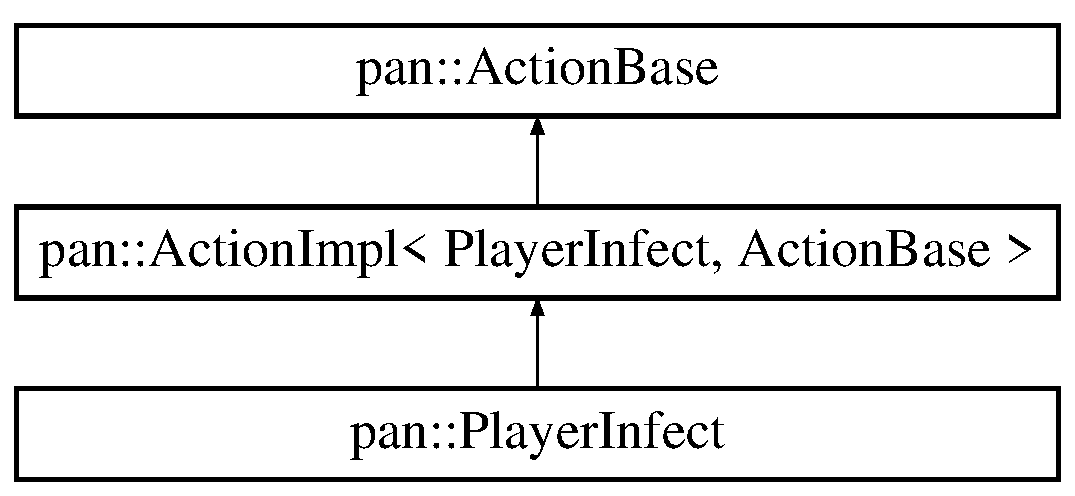
\includegraphics[height=3.000000cm]{classpan_1_1_player_infect}
\end{center}
\end{figure}
\subsection*{Public Member Functions}
\begin{DoxyCompactItemize}
\item 
\hyperlink{classpan_1_1_player_infect_afaa2f602426d0e215d93960bc965ace1}{Player\+Infect} (\hyperlink{namespacepan_a0cdabf874fbf1bb3a1f0152d108c2909}{Player\+Index} \hyperlink{classpan_1_1_player_infect_a315aa72113a32fe97b91ada9df0ccfa6}{player})
\end{DoxyCompactItemize}
\subsection*{Public Attributes}
\begin{DoxyCompactItemize}
\item 
\hyperlink{namespacepan_a0cdabf874fbf1bb3a1f0152d108c2909}{Player\+Index} \hyperlink{classpan_1_1_player_infect_a315aa72113a32fe97b91ada9df0ccfa6}{player}
\end{DoxyCompactItemize}


\subsection{Detailed Description}
Class representing the infect action initiated by the player. Note it is different from the \hyperlink{classpan_1_1_infect}{Infect} action as it does not take any parameters besides the initiatin player\textquotesingle{}s index. 

\begin{DoxyAuthor}{Author}
Hrachya Hakobyan 
\end{DoxyAuthor}


\subsection{Constructor \& Destructor Documentation}
\mbox{\Hypertarget{classpan_1_1_player_infect_afaa2f602426d0e215d93960bc965ace1}\label{classpan_1_1_player_infect_afaa2f602426d0e215d93960bc965ace1}} 
\index{pan\+::\+Player\+Infect@{pan\+::\+Player\+Infect}!Player\+Infect@{Player\+Infect}}
\index{Player\+Infect@{Player\+Infect}!pan\+::\+Player\+Infect@{pan\+::\+Player\+Infect}}
\subsubsection{\texorpdfstring{Player\+Infect()}{PlayerInfect()}}
{\footnotesize\ttfamily pan\+::\+Player\+Infect\+::\+Player\+Infect (\begin{DoxyParamCaption}\item[{\hyperlink{namespacepan_a0cdabf874fbf1bb3a1f0152d108c2909}{Player\+Index}}]{player }\end{DoxyParamCaption})}



\subsection{Member Data Documentation}
\mbox{\Hypertarget{classpan_1_1_player_infect_a315aa72113a32fe97b91ada9df0ccfa6}\label{classpan_1_1_player_infect_a315aa72113a32fe97b91ada9df0ccfa6}} 
\index{pan\+::\+Player\+Infect@{pan\+::\+Player\+Infect}!player@{player}}
\index{player@{player}!pan\+::\+Player\+Infect@{pan\+::\+Player\+Infect}}
\subsubsection{\texorpdfstring{player}{player}}
{\footnotesize\ttfamily \hyperlink{namespacepan_a0cdabf874fbf1bb3a1f0152d108c2909}{Player\+Index} pan\+::\+Player\+Infect\+::player}



The documentation for this class was generated from the following files\+:\begin{DoxyCompactItemize}
\item 
\hyperlink{_player_infect_8h}{Player\+Infect.\+h}\item 
\hyperlink{_player_infect_8cpp}{Player\+Infect.\+cpp}\end{DoxyCompactItemize}

\hypertarget{classpan_1_1_reference_card}{}\section{pan\+:\+:Reference\+Card Class Reference}
\label{classpan_1_1_reference_card}\index{pan\+::\+Reference\+Card@{pan\+::\+Reference\+Card}}


Class representing the \hyperlink{classpan_1_1_reference_card}{Reference\+Card}. Note it is not derived from the base Card class since it does not play any role in the game mechanics.  




{\ttfamily \#include $<$Reference\+Card.\+h$>$}

\subsection*{Public Member Functions}
\begin{DoxyCompactItemize}
\item 
\hyperlink{classpan_1_1_reference_card_a6bd8313b5bca442cd17e32c2bf3ca9fc}{Reference\+Card} ()
\end{DoxyCompactItemize}
\subsection*{Public Attributes}
\begin{DoxyCompactItemize}
\item 
const std\+::string \& \hyperlink{classpan_1_1_reference_card_a770a4188e98004fab2b13218f29bde26}{description}
\end{DoxyCompactItemize}


\subsection{Detailed Description}
Class representing the \hyperlink{classpan_1_1_reference_card}{Reference\+Card}. Note it is not derived from the base Card class since it does not play any role in the game mechanics. 

\subsection{Constructor \& Destructor Documentation}
\mbox{\Hypertarget{classpan_1_1_reference_card_a6bd8313b5bca442cd17e32c2bf3ca9fc}\label{classpan_1_1_reference_card_a6bd8313b5bca442cd17e32c2bf3ca9fc}} 
\index{pan\+::\+Reference\+Card@{pan\+::\+Reference\+Card}!Reference\+Card@{Reference\+Card}}
\index{Reference\+Card@{Reference\+Card}!pan\+::\+Reference\+Card@{pan\+::\+Reference\+Card}}
\subsubsection{\texorpdfstring{Reference\+Card()}{ReferenceCard()}}
{\footnotesize\ttfamily pan\+::\+Reference\+Card\+::\+Reference\+Card (\begin{DoxyParamCaption}{ }\end{DoxyParamCaption})}



\subsection{Member Data Documentation}
\mbox{\Hypertarget{classpan_1_1_reference_card_a770a4188e98004fab2b13218f29bde26}\label{classpan_1_1_reference_card_a770a4188e98004fab2b13218f29bde26}} 
\index{pan\+::\+Reference\+Card@{pan\+::\+Reference\+Card}!description@{description}}
\index{description@{description}!pan\+::\+Reference\+Card@{pan\+::\+Reference\+Card}}
\subsubsection{\texorpdfstring{description}{description}}
{\footnotesize\ttfamily const std\+::string\& pan\+::\+Reference\+Card\+::description}



The documentation for this class was generated from the following files\+:\begin{DoxyCompactItemize}
\item 
\hyperlink{_reference_card_8h}{Reference\+Card.\+h}\item 
\hyperlink{_reference_card_8cpp}{Reference\+Card.\+cpp}\end{DoxyCompactItemize}

\hypertarget{classpan_1_1_region}{}\section{pan\+:\+:Region Class Reference}
\label{classpan_1_1_region}\index{pan\+::\+Region@{pan\+::\+Region}}


Class to represent a region on the map. Must be default constructible and assignable.  




{\ttfamily \#include $<$Region.\+h$>$}

Inheritance diagram for pan\+:\+:Region\+:\begin{figure}[H]
\begin{center}
\leavevmode
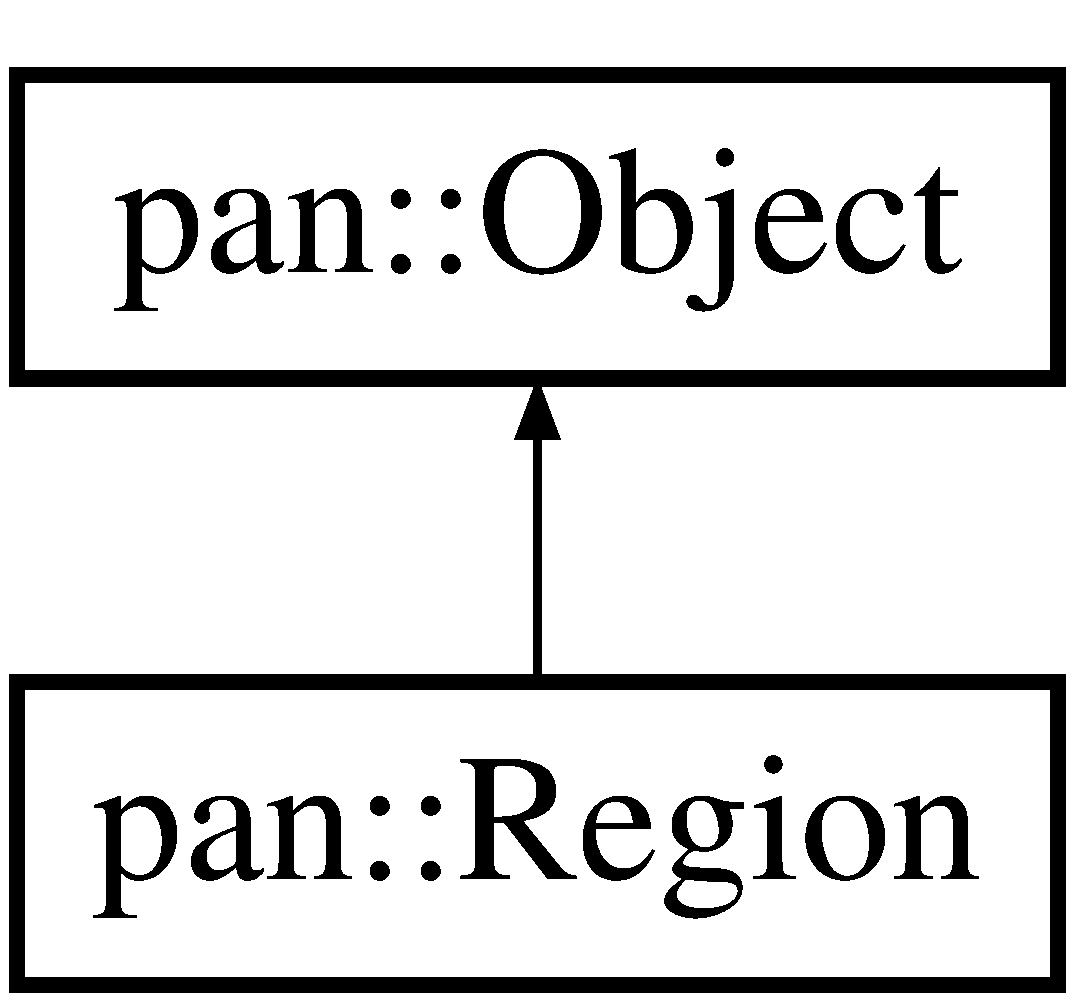
\includegraphics[height=2.000000cm]{classpan_1_1_region}
\end{center}
\end{figure}
\subsection*{Public Member Functions}
\begin{DoxyCompactItemize}
\item 
const std\+::string \& \hyperlink{classpan_1_1_region_a7ebfab047a556e5c95f9a7ea10eb71ba}{get\+Name} () const
\item 
void \hyperlink{classpan_1_1_region_a0138c13e4ba5d07029dd9bb641c8b1ef}{set\+Name} (const std\+::string \&name)
\item 
std\+::string \hyperlink{classpan_1_1_region_abc67a788365510bfad231939713106cb}{description} () const
\item 
bool \hyperlink{classpan_1_1_region_a6f65b58194c83c1c1ec666c6b14c983e}{operator==} (const \hyperlink{classpan_1_1_region}{Region} \&other) const
\item 
bool \hyperlink{classpan_1_1_region_aab9e2291f838d7cf87b2518fa2c1b8a0}{operator!=} (const \hyperlink{classpan_1_1_region}{Region} \&other) const
\item 
{\footnotesize template$<$class Archive $>$ }\\void \hyperlink{classpan_1_1_region_af273dea05ea12be85b8bcdec0e3c22d2}{serialize} (Archive \&ar, const unsigned int)
\end{DoxyCompactItemize}
\subsection*{Friends}
\begin{DoxyCompactItemize}
\item 
class \hyperlink{classpan_1_1_region_ac98d07dd8f7b70e16ccb9a01abf56b9c}{boost\+::serialization\+::access}
\end{DoxyCompactItemize}


\subsection{Detailed Description}
Class to represent a region on the map. Must be default constructible and assignable. 

\begin{DoxyAuthor}{Author}
Hrachya Hakobyan 
\end{DoxyAuthor}


\subsection{Member Function Documentation}
\mbox{\Hypertarget{classpan_1_1_region_abc67a788365510bfad231939713106cb}\label{classpan_1_1_region_abc67a788365510bfad231939713106cb}} 
\index{pan\+::\+Region@{pan\+::\+Region}!description@{description}}
\index{description@{description}!pan\+::\+Region@{pan\+::\+Region}}
\subsubsection{\texorpdfstring{description()}{description()}}
{\footnotesize\ttfamily std\+::string pan\+::\+Region\+::description (\begin{DoxyParamCaption}{ }\end{DoxyParamCaption}) const\hspace{0.3cm}{\ttfamily [inline]}, {\ttfamily [virtual]}}



Implements \hyperlink{classpan_1_1_object_a2bb6d3117bb32f5774657c83f118ed8b}{pan\+::\+Object}.

\mbox{\Hypertarget{classpan_1_1_region_a7ebfab047a556e5c95f9a7ea10eb71ba}\label{classpan_1_1_region_a7ebfab047a556e5c95f9a7ea10eb71ba}} 
\index{pan\+::\+Region@{pan\+::\+Region}!get\+Name@{get\+Name}}
\index{get\+Name@{get\+Name}!pan\+::\+Region@{pan\+::\+Region}}
\subsubsection{\texorpdfstring{get\+Name()}{getName()}}
{\footnotesize\ttfamily const std\+::string \& pan\+::\+Region\+::get\+Name (\begin{DoxyParamCaption}{ }\end{DoxyParamCaption}) const\hspace{0.3cm}{\ttfamily [inline]}}

\mbox{\Hypertarget{classpan_1_1_region_aab9e2291f838d7cf87b2518fa2c1b8a0}\label{classpan_1_1_region_aab9e2291f838d7cf87b2518fa2c1b8a0}} 
\index{pan\+::\+Region@{pan\+::\+Region}!operator"!=@{operator"!=}}
\index{operator"!=@{operator"!=}!pan\+::\+Region@{pan\+::\+Region}}
\subsubsection{\texorpdfstring{operator"!=()}{operator!=()}}
{\footnotesize\ttfamily bool pan\+::\+Region\+::operator!= (\begin{DoxyParamCaption}\item[{const \hyperlink{classpan_1_1_region}{Region} \&}]{other }\end{DoxyParamCaption}) const\hspace{0.3cm}{\ttfamily [inline]}}

\mbox{\Hypertarget{classpan_1_1_region_a6f65b58194c83c1c1ec666c6b14c983e}\label{classpan_1_1_region_a6f65b58194c83c1c1ec666c6b14c983e}} 
\index{pan\+::\+Region@{pan\+::\+Region}!operator==@{operator==}}
\index{operator==@{operator==}!pan\+::\+Region@{pan\+::\+Region}}
\subsubsection{\texorpdfstring{operator==()}{operator==()}}
{\footnotesize\ttfamily bool pan\+::\+Region\+::operator== (\begin{DoxyParamCaption}\item[{const \hyperlink{classpan_1_1_region}{Region} \&}]{other }\end{DoxyParamCaption}) const\hspace{0.3cm}{\ttfamily [inline]}}

\mbox{\Hypertarget{classpan_1_1_region_af273dea05ea12be85b8bcdec0e3c22d2}\label{classpan_1_1_region_af273dea05ea12be85b8bcdec0e3c22d2}} 
\index{pan\+::\+Region@{pan\+::\+Region}!serialize@{serialize}}
\index{serialize@{serialize}!pan\+::\+Region@{pan\+::\+Region}}
\subsubsection{\texorpdfstring{serialize()}{serialize()}}
{\footnotesize\ttfamily template$<$class Archive $>$ \\
void pan\+::\+Region\+::serialize (\begin{DoxyParamCaption}\item[{Archive \&}]{ar,  }\item[{const unsigned}]{int }\end{DoxyParamCaption})\hspace{0.3cm}{\ttfamily [inline]}}

\mbox{\Hypertarget{classpan_1_1_region_a0138c13e4ba5d07029dd9bb641c8b1ef}\label{classpan_1_1_region_a0138c13e4ba5d07029dd9bb641c8b1ef}} 
\index{pan\+::\+Region@{pan\+::\+Region}!set\+Name@{set\+Name}}
\index{set\+Name@{set\+Name}!pan\+::\+Region@{pan\+::\+Region}}
\subsubsection{\texorpdfstring{set\+Name()}{setName()}}
{\footnotesize\ttfamily void pan\+::\+Region\+::set\+Name (\begin{DoxyParamCaption}\item[{const std\+::string \&}]{name }\end{DoxyParamCaption})\hspace{0.3cm}{\ttfamily [inline]}}



\subsection{Friends And Related Function Documentation}
\mbox{\Hypertarget{classpan_1_1_region_ac98d07dd8f7b70e16ccb9a01abf56b9c}\label{classpan_1_1_region_ac98d07dd8f7b70e16ccb9a01abf56b9c}} 
\index{pan\+::\+Region@{pan\+::\+Region}!boost\+::serialization\+::access@{boost\+::serialization\+::access}}
\index{boost\+::serialization\+::access@{boost\+::serialization\+::access}!pan\+::\+Region@{pan\+::\+Region}}
\subsubsection{\texorpdfstring{boost\+::serialization\+::access}{boost::serialization::access}}
{\footnotesize\ttfamily friend class boost\+::serialization\+::access\hspace{0.3cm}{\ttfamily [friend]}}



The documentation for this class was generated from the following file\+:\begin{DoxyCompactItemize}
\item 
\hyperlink{_region_8h}{Region.\+h}\end{DoxyCompactItemize}

\hypertarget{classpan_1_1_role_base}{}\section{pan\+:\+:Role\+Base Class Reference}
\label{classpan_1_1_role_base}\index{pan\+::\+Role\+Base@{pan\+::\+Role\+Base}}


A class to represent the Role entity in the game. The \hyperlink{classpan_1_1_role_base}{Role\+Base} is a the same as the Role card in the real game. The \hyperlink{classpan_1_1_role_base}{Role\+Base} is a prent class to concrete Role classes. The Rol\+Base is not abstract, however it cannot be instantiated because of protected constructor.  




{\ttfamily \#include $<$Role.\+h$>$}

Inheritance diagram for pan\+:\+:Role\+Base\+:\begin{figure}[H]
\begin{center}
\leavevmode
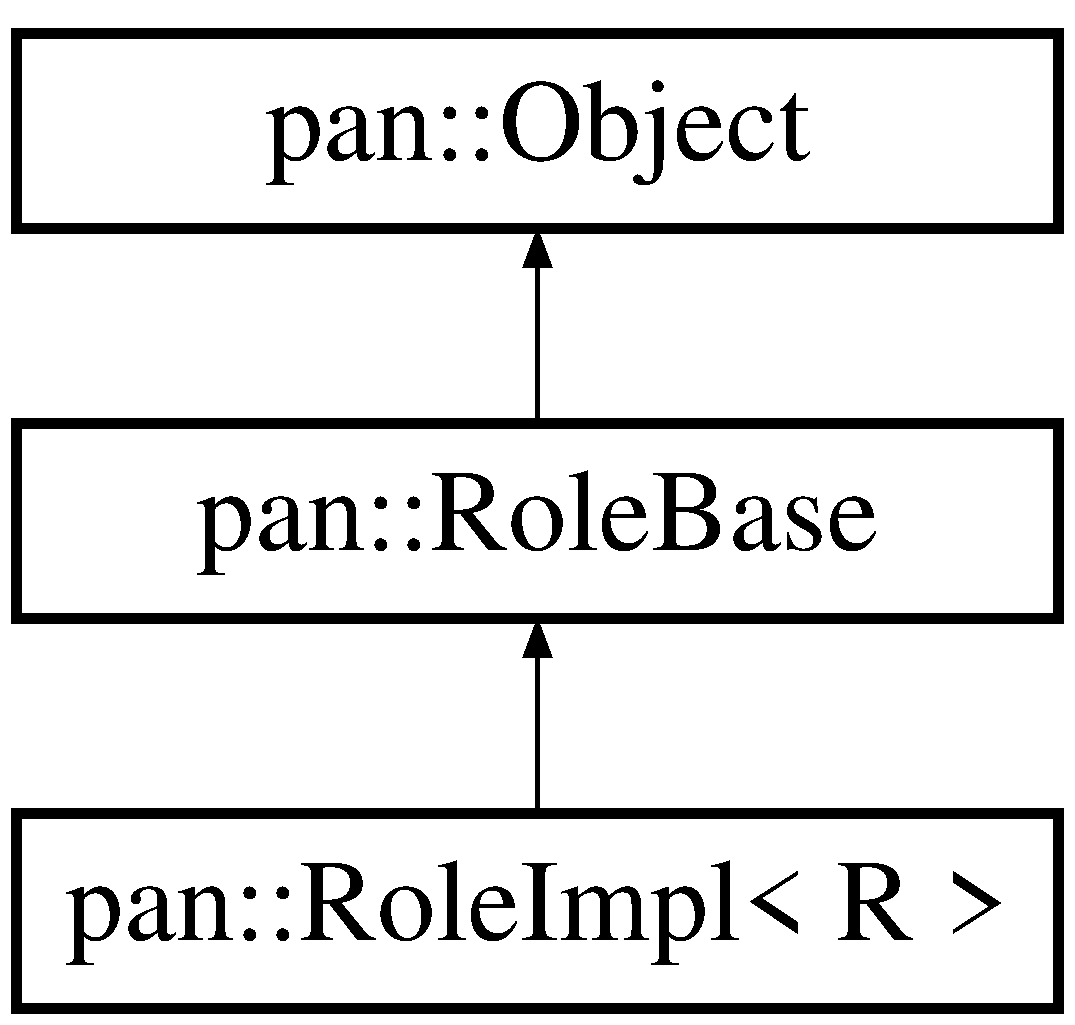
\includegraphics[height=3.000000cm]{classpan_1_1_role_base}
\end{center}
\end{figure}
\subsection*{Public Member Functions}
\begin{DoxyCompactItemize}
\item 
virtual \hyperlink{classpan_1_1_role_base_a6573ddc4f609c21035b7d0e383a01ba8}{$\sim$\+Role\+Base} ()
\item 
bool \hyperlink{classpan_1_1_role_base_aa92715dd7056ec28fa2e6be60c5f8ab5}{operator==} (const \hyperlink{classpan_1_1_role_base}{Role\+Base} \&) const
\item 
bool \hyperlink{classpan_1_1_role_base_a1d3a036dfc74bb7e3a6b9fcdbaaf3ef0}{operator!=} (const \hyperlink{classpan_1_1_role_base}{Role\+Base} \&) const
\item 
std\+::string \hyperlink{classpan_1_1_role_base_a6f4774e52750478d865c4627fc4d4460}{description} () const
\end{DoxyCompactItemize}
\subsection*{Public Attributes}
\begin{DoxyCompactItemize}
\item 
const \hyperlink{namespacepan_a5017f84fa51152eae453759537d1ced6}{Roles} \hyperlink{classpan_1_1_role_base_a1da6d8a75410162b2fc40f05a0b594c9}{role}
\end{DoxyCompactItemize}
\subsection*{Protected Member Functions}
\begin{DoxyCompactItemize}
\item 
\hyperlink{classpan_1_1_role_base_af5df3999e33323806909b0d6d190cecc}{Role\+Base} (\hyperlink{namespacepan_a5017f84fa51152eae453759537d1ced6}{Roles} \hyperlink{classpan_1_1_role_base_a1da6d8a75410162b2fc40f05a0b594c9}{role})
\end{DoxyCompactItemize}


\subsection{Detailed Description}
A class to represent the Role entity in the game. The \hyperlink{classpan_1_1_role_base}{Role\+Base} is a the same as the Role card in the real game. The \hyperlink{classpan_1_1_role_base}{Role\+Base} is a prent class to concrete Role classes. The Rol\+Base is not abstract, however it cannot be instantiated because of protected constructor. 

\begin{DoxyAuthor}{Author}
Hrachya Hakobyan 
\end{DoxyAuthor}


\subsection{Constructor \& Destructor Documentation}
\mbox{\Hypertarget{classpan_1_1_role_base_a6573ddc4f609c21035b7d0e383a01ba8}\label{classpan_1_1_role_base_a6573ddc4f609c21035b7d0e383a01ba8}} 
\index{pan\+::\+Role\+Base@{pan\+::\+Role\+Base}!````~Role\+Base@{$\sim$\+Role\+Base}}
\index{````~Role\+Base@{$\sim$\+Role\+Base}!pan\+::\+Role\+Base@{pan\+::\+Role\+Base}}
\subsubsection{\texorpdfstring{$\sim$\+Role\+Base()}{~RoleBase()}}
{\footnotesize\ttfamily pan\+::\+Role\+Base\+::$\sim$\+Role\+Base (\begin{DoxyParamCaption}{ }\end{DoxyParamCaption})\hspace{0.3cm}{\ttfamily [virtual]}}

\mbox{\Hypertarget{classpan_1_1_role_base_af5df3999e33323806909b0d6d190cecc}\label{classpan_1_1_role_base_af5df3999e33323806909b0d6d190cecc}} 
\index{pan\+::\+Role\+Base@{pan\+::\+Role\+Base}!Role\+Base@{Role\+Base}}
\index{Role\+Base@{Role\+Base}!pan\+::\+Role\+Base@{pan\+::\+Role\+Base}}
\subsubsection{\texorpdfstring{Role\+Base()}{RoleBase()}}
{\footnotesize\ttfamily pan\+::\+Role\+Base\+::\+Role\+Base (\begin{DoxyParamCaption}\item[{\hyperlink{namespacepan_a5017f84fa51152eae453759537d1ced6}{Roles}}]{role }\end{DoxyParamCaption})\hspace{0.3cm}{\ttfamily [protected]}}



\subsection{Member Function Documentation}
\mbox{\Hypertarget{classpan_1_1_role_base_a6f4774e52750478d865c4627fc4d4460}\label{classpan_1_1_role_base_a6f4774e52750478d865c4627fc4d4460}} 
\index{pan\+::\+Role\+Base@{pan\+::\+Role\+Base}!description@{description}}
\index{description@{description}!pan\+::\+Role\+Base@{pan\+::\+Role\+Base}}
\subsubsection{\texorpdfstring{description()}{description()}}
{\footnotesize\ttfamily std\+::string pan\+::\+Role\+Base\+::description (\begin{DoxyParamCaption}{ }\end{DoxyParamCaption}) const\hspace{0.3cm}{\ttfamily [inline]}, {\ttfamily [virtual]}}



Implements \hyperlink{classpan_1_1_object_a2bb6d3117bb32f5774657c83f118ed8b}{pan\+::\+Object}.

\mbox{\Hypertarget{classpan_1_1_role_base_a1d3a036dfc74bb7e3a6b9fcdbaaf3ef0}\label{classpan_1_1_role_base_a1d3a036dfc74bb7e3a6b9fcdbaaf3ef0}} 
\index{pan\+::\+Role\+Base@{pan\+::\+Role\+Base}!operator"!=@{operator"!=}}
\index{operator"!=@{operator"!=}!pan\+::\+Role\+Base@{pan\+::\+Role\+Base}}
\subsubsection{\texorpdfstring{operator"!=()}{operator!=()}}
{\footnotesize\ttfamily bool pan\+::\+Role\+Base\+::operator!= (\begin{DoxyParamCaption}\item[{const \hyperlink{classpan_1_1_role_base}{Role\+Base} \&}]{r }\end{DoxyParamCaption}) const\hspace{0.3cm}{\ttfamily [inline]}}

\mbox{\Hypertarget{classpan_1_1_role_base_aa92715dd7056ec28fa2e6be60c5f8ab5}\label{classpan_1_1_role_base_aa92715dd7056ec28fa2e6be60c5f8ab5}} 
\index{pan\+::\+Role\+Base@{pan\+::\+Role\+Base}!operator==@{operator==}}
\index{operator==@{operator==}!pan\+::\+Role\+Base@{pan\+::\+Role\+Base}}
\subsubsection{\texorpdfstring{operator==()}{operator==()}}
{\footnotesize\ttfamily bool pan\+::\+Role\+Base\+::operator== (\begin{DoxyParamCaption}\item[{const \hyperlink{classpan_1_1_role_base}{Role\+Base} \&}]{r }\end{DoxyParamCaption}) const\hspace{0.3cm}{\ttfamily [inline]}}



\subsection{Member Data Documentation}
\mbox{\Hypertarget{classpan_1_1_role_base_a1da6d8a75410162b2fc40f05a0b594c9}\label{classpan_1_1_role_base_a1da6d8a75410162b2fc40f05a0b594c9}} 
\index{pan\+::\+Role\+Base@{pan\+::\+Role\+Base}!role@{role}}
\index{role@{role}!pan\+::\+Role\+Base@{pan\+::\+Role\+Base}}
\subsubsection{\texorpdfstring{role}{role}}
{\footnotesize\ttfamily const \hyperlink{namespacepan_a5017f84fa51152eae453759537d1ced6}{Roles} pan\+::\+Role\+Base\+::role}



The documentation for this class was generated from the following files\+:\begin{DoxyCompactItemize}
\item 
\hyperlink{_role_8h}{Role.\+h}\item 
\hyperlink{_role_8cpp}{Role.\+cpp}\end{DoxyCompactItemize}

\hypertarget{classpan_1_1_role_impl}{}\section{pan\+:\+:Role\+Impl$<$ R $>$ Class Template Reference}
\label{classpan_1_1_role_impl}\index{pan\+::\+Role\+Impl$<$ R $>$@{pan\+::\+Role\+Impl$<$ R $>$}}


\hyperlink{classpan_1_1_role_impl}{Role\+Impl} is a templated class for concrete Role-\/s. Its template parameter is an Roles enum value.  




{\ttfamily \#include $<$Role.\+h$>$}

Inheritance diagram for pan\+:\+:Role\+Impl$<$ R $>$\+:\begin{figure}[H]
\begin{center}
\leavevmode
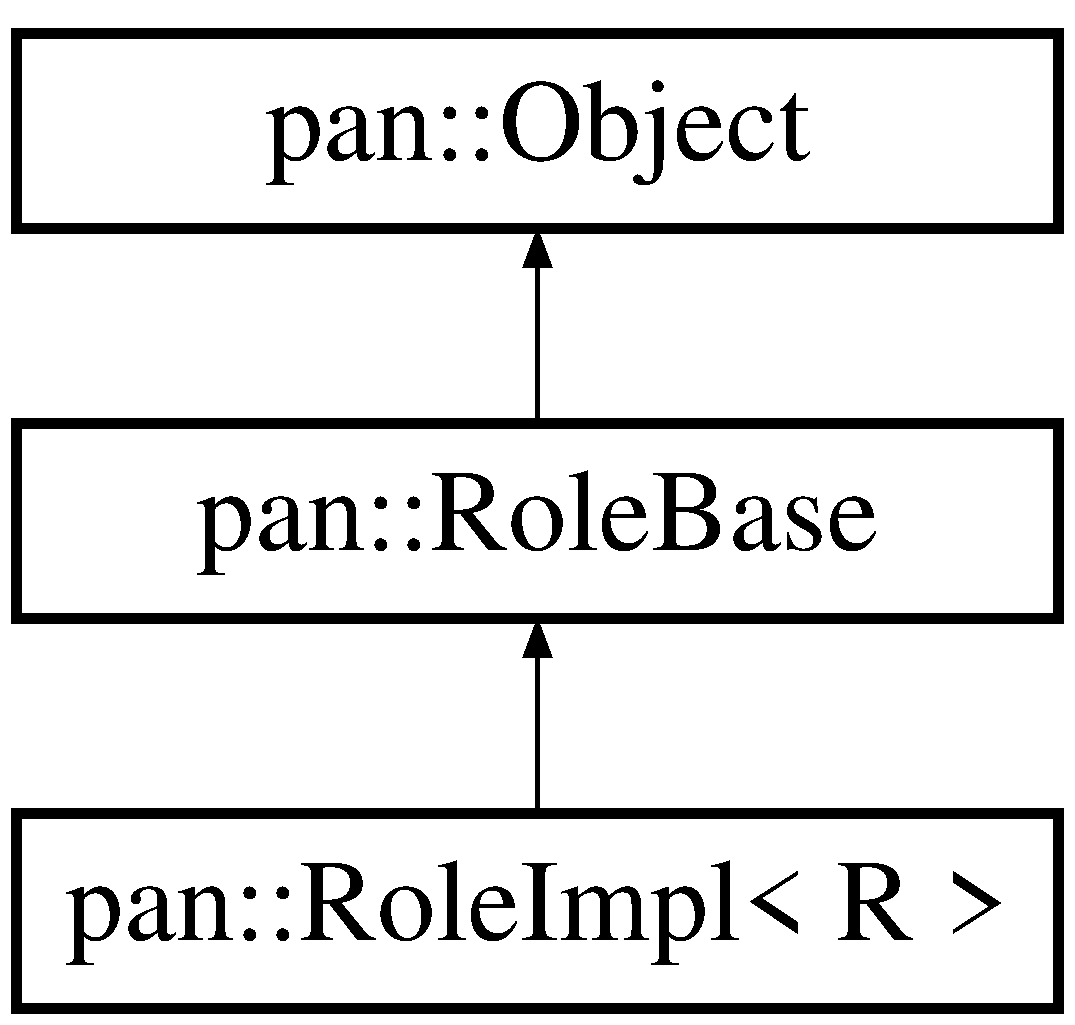
\includegraphics[height=3.000000cm]{classpan_1_1_role_impl}
\end{center}
\end{figure}
\subsection*{Public Member Functions}
\begin{DoxyCompactItemize}
\item 
\hyperlink{classpan_1_1_role_impl_aa747c97282c72f41398e99a6fbdb62ae}{Role\+Impl} ()
\end{DoxyCompactItemize}
\subsection*{Additional Inherited Members}


\subsection{Detailed Description}
\subsubsection*{template$<$Roles R$>$\newline
class pan\+::\+Role\+Impl$<$ R $>$}

\hyperlink{classpan_1_1_role_impl}{Role\+Impl} is a templated class for concrete Role-\/s. Its template parameter is an Roles enum value. 

\subsection{Constructor \& Destructor Documentation}
\mbox{\Hypertarget{classpan_1_1_role_impl_aa747c97282c72f41398e99a6fbdb62ae}\label{classpan_1_1_role_impl_aa747c97282c72f41398e99a6fbdb62ae}} 
\index{pan\+::\+Role\+Impl@{pan\+::\+Role\+Impl}!Role\+Impl@{Role\+Impl}}
\index{Role\+Impl@{Role\+Impl}!pan\+::\+Role\+Impl@{pan\+::\+Role\+Impl}}
\subsubsection{\texorpdfstring{Role\+Impl()}{RoleImpl()}}
{\footnotesize\ttfamily template$<$Roles R$>$ \\
\hyperlink{classpan_1_1_role_impl}{pan\+::\+Role\+Impl}$<$ R $>$\+::\hyperlink{classpan_1_1_role_impl}{Role\+Impl} (\begin{DoxyParamCaption}{ }\end{DoxyParamCaption})}



The documentation for this class was generated from the following file\+:\begin{DoxyCompactItemize}
\item 
\hyperlink{_role_8h}{Role.\+h}\end{DoxyCompactItemize}

\hypertarget{classpan_1_1_settings}{}\section{pan\+:\+:Settings Class Reference}
\label{classpan_1_1_settings}\index{pan\+::\+Settings@{pan\+::\+Settings}}


encapsulates all game related parameters.  




{\ttfamily \#include $<$Settings.\+h$>$}

Inheritance diagram for pan\+:\+:Settings\+:\begin{figure}[H]
\begin{center}
\leavevmode
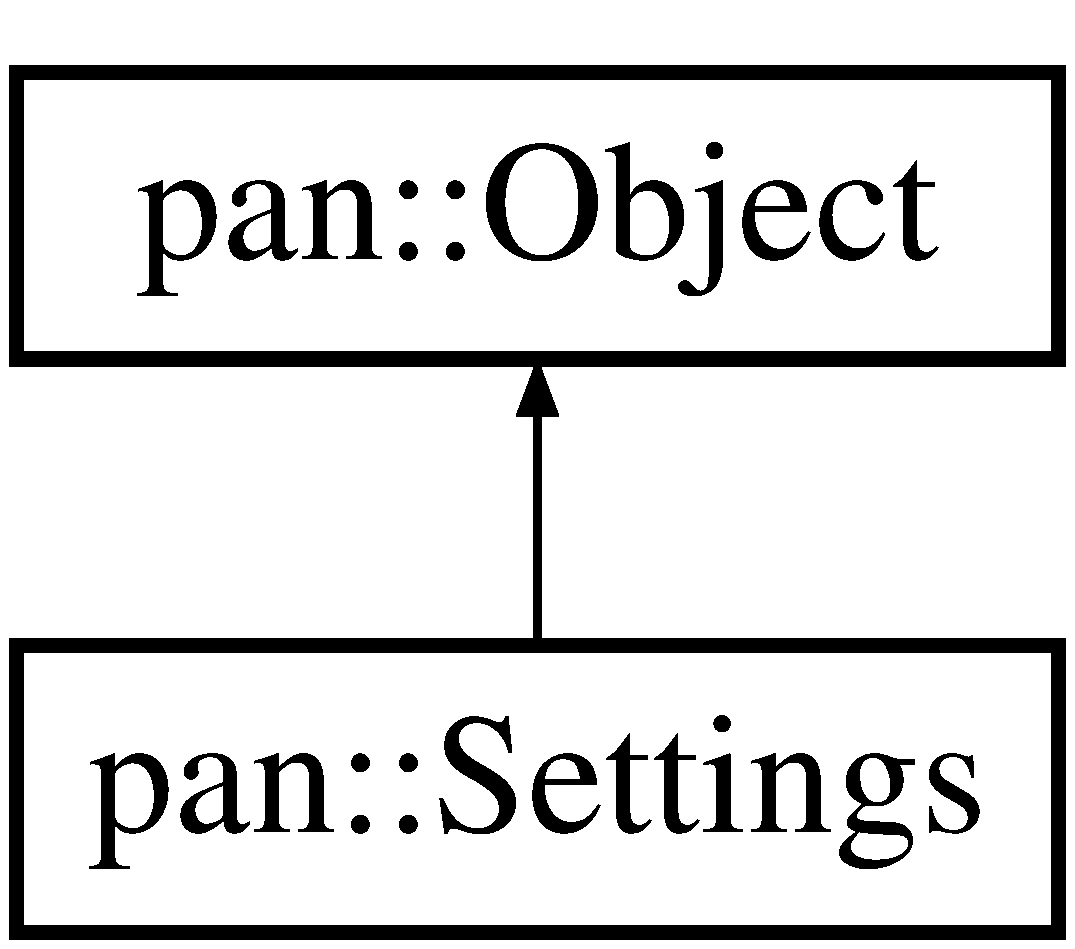
\includegraphics[height=2.000000cm]{classpan_1_1_settings}
\end{center}
\end{figure}
\subsection*{Public Member Functions}
\begin{DoxyCompactItemize}
\item 
\hyperlink{classpan_1_1_settings_af5bdfa4c3ed9460b0290d9f3d0aee02a}{Settings} ()
\item 
\hyperlink{classpan_1_1_settings_a88e5d34527d110fd6391df762199c405}{Settings} (unsigned int \hyperlink{classpan_1_1_settings_a4a7c2963d63bd768b9e64ffb8461333f}{player\+Count}, unsigned int \hyperlink{classpan_1_1_settings_a61569c8a2fcccdf9409d5467625ee788}{epidemic\+Card\+Count}, unsigned int \hyperlink{classpan_1_1_settings_adf8144ec33fa2217b8fc422e7b4806be}{initial\+Cards})
\item 
\hyperlink{classpan_1_1_settings_a73b85e961b1be7a48d5cca58c9a61f41}{$\sim$\+Settings} ()=default
\item 
std\+::string \hyperlink{classpan_1_1_settings_ac88db54a696993babc9c495d54fc89c3}{description} () const
\item 
bool \hyperlink{classpan_1_1_settings_a5a068817d5e6f48ac72b9f2706f185a8}{operator==} (const \hyperlink{classpan_1_1_settings}{Settings} \&) const
\item 
bool \hyperlink{classpan_1_1_settings_a47b2bc896ccc1de8ab00f734555b4cdc}{operator!=} (const \hyperlink{classpan_1_1_settings}{Settings} \&) const
\end{DoxyCompactItemize}
\subsection*{Static Public Member Functions}
\begin{DoxyCompactItemize}
\item 
static \hyperlink{classpan_1_1_settings}{Settings} \hyperlink{classpan_1_1_settings_a908b6305091cf8d02bb4179dcbbe4ad1}{Beginner} (unsigned int players)
\item 
static \hyperlink{classpan_1_1_settings}{Settings} \hyperlink{classpan_1_1_settings_a272d0e01c6e60dcfa1958c9ae54ff69f}{Standard} (unsigned int players)
\item 
static \hyperlink{classpan_1_1_settings}{Settings} \hyperlink{classpan_1_1_settings_af0212489163b1d55fc5e661ad85a0b1e}{Heroic} (unsigned int players)
\end{DoxyCompactItemize}
\subsection*{Public Attributes}
\begin{DoxyCompactItemize}
\item 
unsigned int \hyperlink{classpan_1_1_settings_a4a7c2963d63bd768b9e64ffb8461333f}{player\+Count}
\item 
unsigned int \hyperlink{classpan_1_1_settings_a61569c8a2fcccdf9409d5467625ee788}{epidemic\+Card\+Count}
\item 
unsigned int \hyperlink{classpan_1_1_settings_adf8144ec33fa2217b8fc422e7b4806be}{initial\+Cards}
\item 
unsigned int \hyperlink{classpan_1_1_settings_adb30d858a479ca96e0f7d3591bf77746}{player\+Draw\+Count} = 2
\item 
unsigned int \hyperlink{classpan_1_1_settings_a6702806d498f37822811241a2a8f7ab3}{discover\+Cure\+Card\+Count} = 5
\item 
unsigned int \hyperlink{classpan_1_1_settings_a189fdd9a58dc25ca3f8766be031eba99}{player\+Hand\+Max} = 7
\item 
unsigned int \hyperlink{classpan_1_1_settings_a85ce29ab84bb000a19f31eb00c7134ed}{disease\+Cubes\+Per\+Disease} = 24
\item 
unsigned int \hyperlink{classpan_1_1_settings_ab3fc24065a6f74fc63a6f171ffc8fea2}{max\+Research\+Stations} = 6
\item 
unsigned int \hyperlink{classpan_1_1_settings_a437e7eaf47786919ebd3504100d5ac68}{outbreak\+Marker\+Max} = 8
\item 
std\+::vector$<$ unsigned int $>$ \hyperlink{classpan_1_1_settings_a9b9d37ca162c63ab759271fd21e7b15f}{infection\+Rates}
\end{DoxyCompactItemize}
\subsection*{Friends}
\begin{DoxyCompactItemize}
\item 
class \hyperlink{classpan_1_1_settings_ac98d07dd8f7b70e16ccb9a01abf56b9c}{boost\+::serialization\+::access}
\end{DoxyCompactItemize}


\subsection{Detailed Description}
encapsulates all game related parameters. 

\begin{DoxyAuthor}{Author}
Hrachya Hakobyan 
\end{DoxyAuthor}


\subsection{Constructor \& Destructor Documentation}
\mbox{\Hypertarget{classpan_1_1_settings_af5bdfa4c3ed9460b0290d9f3d0aee02a}\label{classpan_1_1_settings_af5bdfa4c3ed9460b0290d9f3d0aee02a}} 
\index{pan\+::\+Settings@{pan\+::\+Settings}!Settings@{Settings}}
\index{Settings@{Settings}!pan\+::\+Settings@{pan\+::\+Settings}}
\subsubsection{\texorpdfstring{Settings()}{Settings()}\hspace{0.1cm}{\footnotesize\ttfamily [1/2]}}
{\footnotesize\ttfamily pan\+::\+Settings\+::\+Settings (\begin{DoxyParamCaption}{ }\end{DoxyParamCaption})}

\mbox{\Hypertarget{classpan_1_1_settings_a88e5d34527d110fd6391df762199c405}\label{classpan_1_1_settings_a88e5d34527d110fd6391df762199c405}} 
\index{pan\+::\+Settings@{pan\+::\+Settings}!Settings@{Settings}}
\index{Settings@{Settings}!pan\+::\+Settings@{pan\+::\+Settings}}
\subsubsection{\texorpdfstring{Settings()}{Settings()}\hspace{0.1cm}{\footnotesize\ttfamily [2/2]}}
{\footnotesize\ttfamily pan\+::\+Settings\+::\+Settings (\begin{DoxyParamCaption}\item[{unsigned int}]{player\+Count,  }\item[{unsigned int}]{epidemic\+Card\+Count,  }\item[{unsigned int}]{initial\+Cards }\end{DoxyParamCaption})}

\mbox{\Hypertarget{classpan_1_1_settings_a73b85e961b1be7a48d5cca58c9a61f41}\label{classpan_1_1_settings_a73b85e961b1be7a48d5cca58c9a61f41}} 
\index{pan\+::\+Settings@{pan\+::\+Settings}!````~Settings@{$\sim$\+Settings}}
\index{````~Settings@{$\sim$\+Settings}!pan\+::\+Settings@{pan\+::\+Settings}}
\subsubsection{\texorpdfstring{$\sim$\+Settings()}{~Settings()}}
{\footnotesize\ttfamily pan\+::\+Settings\+::$\sim$\+Settings (\begin{DoxyParamCaption}{ }\end{DoxyParamCaption})\hspace{0.3cm}{\ttfamily [default]}}



\subsection{Member Function Documentation}
\mbox{\Hypertarget{classpan_1_1_settings_a908b6305091cf8d02bb4179dcbbe4ad1}\label{classpan_1_1_settings_a908b6305091cf8d02bb4179dcbbe4ad1}} 
\index{pan\+::\+Settings@{pan\+::\+Settings}!Beginner@{Beginner}}
\index{Beginner@{Beginner}!pan\+::\+Settings@{pan\+::\+Settings}}
\subsubsection{\texorpdfstring{Beginner()}{Beginner()}}
{\footnotesize\ttfamily \hyperlink{classpan_1_1_settings}{Settings} pan\+::\+Settings\+::\+Beginner (\begin{DoxyParamCaption}\item[{unsigned int}]{players }\end{DoxyParamCaption})\hspace{0.3cm}{\ttfamily [inline]}, {\ttfamily [static]}}

\mbox{\Hypertarget{classpan_1_1_settings_ac88db54a696993babc9c495d54fc89c3}\label{classpan_1_1_settings_ac88db54a696993babc9c495d54fc89c3}} 
\index{pan\+::\+Settings@{pan\+::\+Settings}!description@{description}}
\index{description@{description}!pan\+::\+Settings@{pan\+::\+Settings}}
\subsubsection{\texorpdfstring{description()}{description()}}
{\footnotesize\ttfamily std\+::string pan\+::\+Settings\+::description (\begin{DoxyParamCaption}{ }\end{DoxyParamCaption}) const\hspace{0.3cm}{\ttfamily [inline]}, {\ttfamily [virtual]}}



Implements \hyperlink{classpan_1_1_object_a2bb6d3117bb32f5774657c83f118ed8b}{pan\+::\+Object}.

\mbox{\Hypertarget{classpan_1_1_settings_af0212489163b1d55fc5e661ad85a0b1e}\label{classpan_1_1_settings_af0212489163b1d55fc5e661ad85a0b1e}} 
\index{pan\+::\+Settings@{pan\+::\+Settings}!Heroic@{Heroic}}
\index{Heroic@{Heroic}!pan\+::\+Settings@{pan\+::\+Settings}}
\subsubsection{\texorpdfstring{Heroic()}{Heroic()}}
{\footnotesize\ttfamily \hyperlink{classpan_1_1_settings}{Settings} pan\+::\+Settings\+::\+Heroic (\begin{DoxyParamCaption}\item[{unsigned int}]{players }\end{DoxyParamCaption})\hspace{0.3cm}{\ttfamily [inline]}, {\ttfamily [static]}}

\mbox{\Hypertarget{classpan_1_1_settings_a47b2bc896ccc1de8ab00f734555b4cdc}\label{classpan_1_1_settings_a47b2bc896ccc1de8ab00f734555b4cdc}} 
\index{pan\+::\+Settings@{pan\+::\+Settings}!operator"!=@{operator"!=}}
\index{operator"!=@{operator"!=}!pan\+::\+Settings@{pan\+::\+Settings}}
\subsubsection{\texorpdfstring{operator"!=()}{operator!=()}}
{\footnotesize\ttfamily bool pan\+::\+Settings\+::operator!= (\begin{DoxyParamCaption}\item[{const \hyperlink{classpan_1_1_settings}{Settings} \&}]{s }\end{DoxyParamCaption}) const}

\mbox{\Hypertarget{classpan_1_1_settings_a5a068817d5e6f48ac72b9f2706f185a8}\label{classpan_1_1_settings_a5a068817d5e6f48ac72b9f2706f185a8}} 
\index{pan\+::\+Settings@{pan\+::\+Settings}!operator==@{operator==}}
\index{operator==@{operator==}!pan\+::\+Settings@{pan\+::\+Settings}}
\subsubsection{\texorpdfstring{operator==()}{operator==()}}
{\footnotesize\ttfamily bool pan\+::\+Settings\+::operator== (\begin{DoxyParamCaption}\item[{const \hyperlink{classpan_1_1_settings}{Settings} \&}]{s }\end{DoxyParamCaption}) const}

\mbox{\Hypertarget{classpan_1_1_settings_a272d0e01c6e60dcfa1958c9ae54ff69f}\label{classpan_1_1_settings_a272d0e01c6e60dcfa1958c9ae54ff69f}} 
\index{pan\+::\+Settings@{pan\+::\+Settings}!Standard@{Standard}}
\index{Standard@{Standard}!pan\+::\+Settings@{pan\+::\+Settings}}
\subsubsection{\texorpdfstring{Standard()}{Standard()}}
{\footnotesize\ttfamily \hyperlink{classpan_1_1_settings}{Settings} pan\+::\+Settings\+::\+Standard (\begin{DoxyParamCaption}\item[{unsigned int}]{players }\end{DoxyParamCaption})\hspace{0.3cm}{\ttfamily [inline]}, {\ttfamily [static]}}



\subsection{Friends And Related Function Documentation}
\mbox{\Hypertarget{classpan_1_1_settings_ac98d07dd8f7b70e16ccb9a01abf56b9c}\label{classpan_1_1_settings_ac98d07dd8f7b70e16ccb9a01abf56b9c}} 
\index{pan\+::\+Settings@{pan\+::\+Settings}!boost\+::serialization\+::access@{boost\+::serialization\+::access}}
\index{boost\+::serialization\+::access@{boost\+::serialization\+::access}!pan\+::\+Settings@{pan\+::\+Settings}}
\subsubsection{\texorpdfstring{boost\+::serialization\+::access}{boost::serialization::access}}
{\footnotesize\ttfamily friend class boost\+::serialization\+::access\hspace{0.3cm}{\ttfamily [friend]}}



\subsection{Member Data Documentation}
\mbox{\Hypertarget{classpan_1_1_settings_a6702806d498f37822811241a2a8f7ab3}\label{classpan_1_1_settings_a6702806d498f37822811241a2a8f7ab3}} 
\index{pan\+::\+Settings@{pan\+::\+Settings}!discover\+Cure\+Card\+Count@{discover\+Cure\+Card\+Count}}
\index{discover\+Cure\+Card\+Count@{discover\+Cure\+Card\+Count}!pan\+::\+Settings@{pan\+::\+Settings}}
\subsubsection{\texorpdfstring{discover\+Cure\+Card\+Count}{discoverCureCardCount}}
{\footnotesize\ttfamily unsigned int pan\+::\+Settings\+::discover\+Cure\+Card\+Count = 5}

Default number of matching cards required to cure a disease \mbox{\Hypertarget{classpan_1_1_settings_a85ce29ab84bb000a19f31eb00c7134ed}\label{classpan_1_1_settings_a85ce29ab84bb000a19f31eb00c7134ed}} 
\index{pan\+::\+Settings@{pan\+::\+Settings}!disease\+Cubes\+Per\+Disease@{disease\+Cubes\+Per\+Disease}}
\index{disease\+Cubes\+Per\+Disease@{disease\+Cubes\+Per\+Disease}!pan\+::\+Settings@{pan\+::\+Settings}}
\subsubsection{\texorpdfstring{disease\+Cubes\+Per\+Disease}{diseaseCubesPerDisease}}
{\footnotesize\ttfamily unsigned int pan\+::\+Settings\+::disease\+Cubes\+Per\+Disease = 24}

Number of disease cubes per disease \mbox{\Hypertarget{classpan_1_1_settings_a61569c8a2fcccdf9409d5467625ee788}\label{classpan_1_1_settings_a61569c8a2fcccdf9409d5467625ee788}} 
\index{pan\+::\+Settings@{pan\+::\+Settings}!epidemic\+Card\+Count@{epidemic\+Card\+Count}}
\index{epidemic\+Card\+Count@{epidemic\+Card\+Count}!pan\+::\+Settings@{pan\+::\+Settings}}
\subsubsection{\texorpdfstring{epidemic\+Card\+Count}{epidemicCardCount}}
{\footnotesize\ttfamily unsigned int pan\+::\+Settings\+::epidemic\+Card\+Count}

Number of epidemic cards \mbox{\Hypertarget{classpan_1_1_settings_a9b9d37ca162c63ab759271fd21e7b15f}\label{classpan_1_1_settings_a9b9d37ca162c63ab759271fd21e7b15f}} 
\index{pan\+::\+Settings@{pan\+::\+Settings}!infection\+Rates@{infection\+Rates}}
\index{infection\+Rates@{infection\+Rates}!pan\+::\+Settings@{pan\+::\+Settings}}
\subsubsection{\texorpdfstring{infection\+Rates}{infectionRates}}
{\footnotesize\ttfamily std\+::vector$<$unsigned int$>$ pan\+::\+Settings\+::infection\+Rates}

The infection rates for a give infection rate marker \mbox{\Hypertarget{classpan_1_1_settings_adf8144ec33fa2217b8fc422e7b4806be}\label{classpan_1_1_settings_adf8144ec33fa2217b8fc422e7b4806be}} 
\index{pan\+::\+Settings@{pan\+::\+Settings}!initial\+Cards@{initial\+Cards}}
\index{initial\+Cards@{initial\+Cards}!pan\+::\+Settings@{pan\+::\+Settings}}
\subsubsection{\texorpdfstring{initial\+Cards}{initialCards}}
{\footnotesize\ttfamily unsigned int pan\+::\+Settings\+::initial\+Cards}

Initial number of cards of each player \mbox{\Hypertarget{classpan_1_1_settings_ab3fc24065a6f74fc63a6f171ffc8fea2}\label{classpan_1_1_settings_ab3fc24065a6f74fc63a6f171ffc8fea2}} 
\index{pan\+::\+Settings@{pan\+::\+Settings}!max\+Research\+Stations@{max\+Research\+Stations}}
\index{max\+Research\+Stations@{max\+Research\+Stations}!pan\+::\+Settings@{pan\+::\+Settings}}
\subsubsection{\texorpdfstring{max\+Research\+Stations}{maxResearchStations}}
{\footnotesize\ttfamily unsigned int pan\+::\+Settings\+::max\+Research\+Stations = 6}

Maximum number of research stations \mbox{\Hypertarget{classpan_1_1_settings_a437e7eaf47786919ebd3504100d5ac68}\label{classpan_1_1_settings_a437e7eaf47786919ebd3504100d5ac68}} 
\index{pan\+::\+Settings@{pan\+::\+Settings}!outbreak\+Marker\+Max@{outbreak\+Marker\+Max}}
\index{outbreak\+Marker\+Max@{outbreak\+Marker\+Max}!pan\+::\+Settings@{pan\+::\+Settings}}
\subsubsection{\texorpdfstring{outbreak\+Marker\+Max}{outbreakMarkerMax}}
{\footnotesize\ttfamily unsigned int pan\+::\+Settings\+::outbreak\+Marker\+Max = 8}

Maximum value of the outbreak marker \mbox{\Hypertarget{classpan_1_1_settings_a4a7c2963d63bd768b9e64ffb8461333f}\label{classpan_1_1_settings_a4a7c2963d63bd768b9e64ffb8461333f}} 
\index{pan\+::\+Settings@{pan\+::\+Settings}!player\+Count@{player\+Count}}
\index{player\+Count@{player\+Count}!pan\+::\+Settings@{pan\+::\+Settings}}
\subsubsection{\texorpdfstring{player\+Count}{playerCount}}
{\footnotesize\ttfamily unsigned int pan\+::\+Settings\+::player\+Count}

Number of players \mbox{\Hypertarget{classpan_1_1_settings_adb30d858a479ca96e0f7d3591bf77746}\label{classpan_1_1_settings_adb30d858a479ca96e0f7d3591bf77746}} 
\index{pan\+::\+Settings@{pan\+::\+Settings}!player\+Draw\+Count@{player\+Draw\+Count}}
\index{player\+Draw\+Count@{player\+Draw\+Count}!pan\+::\+Settings@{pan\+::\+Settings}}
\subsubsection{\texorpdfstring{player\+Draw\+Count}{playerDrawCount}}
{\footnotesize\ttfamily unsigned int pan\+::\+Settings\+::player\+Draw\+Count = 2}

Number of cards to be drawn by each player \mbox{\Hypertarget{classpan_1_1_settings_a189fdd9a58dc25ca3f8766be031eba99}\label{classpan_1_1_settings_a189fdd9a58dc25ca3f8766be031eba99}} 
\index{pan\+::\+Settings@{pan\+::\+Settings}!player\+Hand\+Max@{player\+Hand\+Max}}
\index{player\+Hand\+Max@{player\+Hand\+Max}!pan\+::\+Settings@{pan\+::\+Settings}}
\subsubsection{\texorpdfstring{player\+Hand\+Max}{playerHandMax}}
{\footnotesize\ttfamily unsigned int pan\+::\+Settings\+::player\+Hand\+Max = 7}

Size of the player hand 

The documentation for this class was generated from the following files\+:\begin{DoxyCompactItemize}
\item 
\hyperlink{_settings_8h}{Settings.\+h}\item 
\hyperlink{_settings_8cpp}{Settings.\+cpp}\end{DoxyCompactItemize}

\hypertarget{classpan_1_1_shuttle_flight}{}\section{pan\+:\+:Shuttle\+Flight Class Reference}
\label{classpan_1_1_shuttle_flight}\index{pan\+::\+Shuttle\+Flight@{pan\+::\+Shuttle\+Flight}}


Class representing a shuttle flight action.  




{\ttfamily \#include $<$Shuttle\+Flight.\+h$>$}

Inheritance diagram for pan\+:\+:Shuttle\+Flight\+:\begin{figure}[H]
\begin{center}
\leavevmode
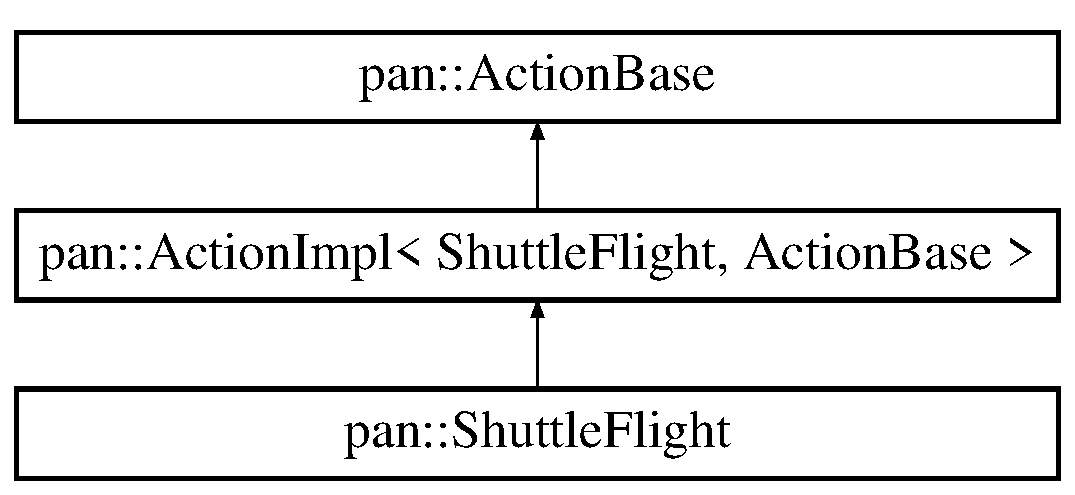
\includegraphics[height=3.000000cm]{classpan_1_1_shuttle_flight}
\end{center}
\end{figure}
\subsection*{Public Member Functions}
\begin{DoxyCompactItemize}
\item 
\hyperlink{classpan_1_1_shuttle_flight_af5deefa81bd19d0fd0776a43c045067a}{Shuttle\+Flight} (\hyperlink{namespacepan_a0cdabf874fbf1bb3a1f0152d108c2909}{Player\+Index} \hyperlink{classpan_1_1_shuttle_flight_a50cd09f3860cdfb821d676dd59c09949}{player}, \hyperlink{namespacepan_afaed28aa6603153dcc062a028602d697}{City\+Index} city)
\end{DoxyCompactItemize}
\subsection*{Public Attributes}
\begin{DoxyCompactItemize}
\item 
\hyperlink{namespacepan_a0cdabf874fbf1bb3a1f0152d108c2909}{Player\+Index} \hyperlink{classpan_1_1_shuttle_flight_a50cd09f3860cdfb821d676dd59c09949}{player}
\item 
\hyperlink{namespacepan_afaed28aa6603153dcc062a028602d697}{City\+Index} \hyperlink{classpan_1_1_shuttle_flight_ac32722c319ed43587c2374109c70f734}{target\+City}
\end{DoxyCompactItemize}


\subsection{Detailed Description}
Class representing a shuttle flight action. 

\begin{DoxyAuthor}{Author}
Hrachya Hakobyan 
\end{DoxyAuthor}


\subsection{Constructor \& Destructor Documentation}
\mbox{\Hypertarget{classpan_1_1_shuttle_flight_af5deefa81bd19d0fd0776a43c045067a}\label{classpan_1_1_shuttle_flight_af5deefa81bd19d0fd0776a43c045067a}} 
\index{pan\+::\+Shuttle\+Flight@{pan\+::\+Shuttle\+Flight}!Shuttle\+Flight@{Shuttle\+Flight}}
\index{Shuttle\+Flight@{Shuttle\+Flight}!pan\+::\+Shuttle\+Flight@{pan\+::\+Shuttle\+Flight}}
\subsubsection{\texorpdfstring{Shuttle\+Flight()}{ShuttleFlight()}}
{\footnotesize\ttfamily pan\+::\+Shuttle\+Flight\+::\+Shuttle\+Flight (\begin{DoxyParamCaption}\item[{\hyperlink{namespacepan_a0cdabf874fbf1bb3a1f0152d108c2909}{Player\+Index}}]{player,  }\item[{\hyperlink{namespacepan_afaed28aa6603153dcc062a028602d697}{City\+Index}}]{city }\end{DoxyParamCaption})}



\subsection{Member Data Documentation}
\mbox{\Hypertarget{classpan_1_1_shuttle_flight_a50cd09f3860cdfb821d676dd59c09949}\label{classpan_1_1_shuttle_flight_a50cd09f3860cdfb821d676dd59c09949}} 
\index{pan\+::\+Shuttle\+Flight@{pan\+::\+Shuttle\+Flight}!player@{player}}
\index{player@{player}!pan\+::\+Shuttle\+Flight@{pan\+::\+Shuttle\+Flight}}
\subsubsection{\texorpdfstring{player}{player}}
{\footnotesize\ttfamily \hyperlink{namespacepan_a0cdabf874fbf1bb3a1f0152d108c2909}{Player\+Index} pan\+::\+Shuttle\+Flight\+::player}

\mbox{\Hypertarget{classpan_1_1_shuttle_flight_ac32722c319ed43587c2374109c70f734}\label{classpan_1_1_shuttle_flight_ac32722c319ed43587c2374109c70f734}} 
\index{pan\+::\+Shuttle\+Flight@{pan\+::\+Shuttle\+Flight}!target\+City@{target\+City}}
\index{target\+City@{target\+City}!pan\+::\+Shuttle\+Flight@{pan\+::\+Shuttle\+Flight}}
\subsubsection{\texorpdfstring{target\+City}{targetCity}}
{\footnotesize\ttfamily \hyperlink{namespacepan_afaed28aa6603153dcc062a028602d697}{City\+Index} pan\+::\+Shuttle\+Flight\+::target\+City}



The documentation for this class was generated from the following files\+:\begin{DoxyCompactItemize}
\item 
\hyperlink{_shuttle_flight_8h}{Shuttle\+Flight.\+h}\item 
\hyperlink{_shuttle_flight_8cpp}{Shuttle\+Flight.\+cpp}\end{DoxyCompactItemize}

\hypertarget{classpan_1_1_treat_disease}{}\section{pan\+:\+:Treat\+Disease Class Reference}
\label{classpan_1_1_treat_disease}\index{pan\+::\+Treat\+Disease@{pan\+::\+Treat\+Disease}}


Class representing a treat disease action.  




{\ttfamily \#include $<$Treat\+Disease.\+h$>$}

Inheritance diagram for pan\+:\+:Treat\+Disease\+:\begin{figure}[H]
\begin{center}
\leavevmode
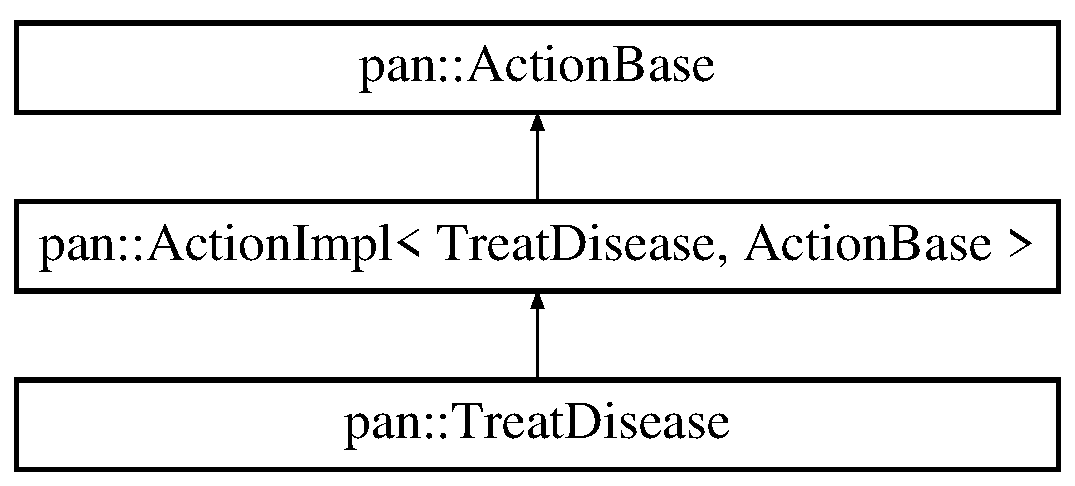
\includegraphics[height=3.000000cm]{classpan_1_1_treat_disease}
\end{center}
\end{figure}
\subsection*{Public Member Functions}
\begin{DoxyCompactItemize}
\item 
\hyperlink{classpan_1_1_treat_disease_a5c47ff414235ac559fb2236ddb00dcaa}{Treat\+Disease} (\hyperlink{namespacepan_a0cdabf874fbf1bb3a1f0152d108c2909}{Player\+Index} \hyperlink{classpan_1_1_treat_disease_a03aa74052746dc12d607458b260281db}{player}, \hyperlink{namespacepan_a48851b51b0aef3f0e1be80df5031d9d7}{Disease\+Type} d\+Type)
\end{DoxyCompactItemize}
\subsection*{Public Attributes}
\begin{DoxyCompactItemize}
\item 
\hyperlink{namespacepan_a0cdabf874fbf1bb3a1f0152d108c2909}{Player\+Index} \hyperlink{classpan_1_1_treat_disease_a03aa74052746dc12d607458b260281db}{player}
\item 
\hyperlink{namespacepan_a48851b51b0aef3f0e1be80df5031d9d7}{Disease\+Type} \hyperlink{classpan_1_1_treat_disease_a9ab5c64aa8c996c62a25b6f1fdf1d4c6}{disease\+Type}
\end{DoxyCompactItemize}


\subsection{Detailed Description}
Class representing a treat disease action. 

\begin{DoxyAuthor}{Author}
Hrachya Hakobyan 
\end{DoxyAuthor}


\subsection{Constructor \& Destructor Documentation}
\mbox{\Hypertarget{classpan_1_1_treat_disease_a5c47ff414235ac559fb2236ddb00dcaa}\label{classpan_1_1_treat_disease_a5c47ff414235ac559fb2236ddb00dcaa}} 
\index{pan\+::\+Treat\+Disease@{pan\+::\+Treat\+Disease}!Treat\+Disease@{Treat\+Disease}}
\index{Treat\+Disease@{Treat\+Disease}!pan\+::\+Treat\+Disease@{pan\+::\+Treat\+Disease}}
\subsubsection{\texorpdfstring{Treat\+Disease()}{TreatDisease()}}
{\footnotesize\ttfamily pan\+::\+Treat\+Disease\+::\+Treat\+Disease (\begin{DoxyParamCaption}\item[{\hyperlink{namespacepan_a0cdabf874fbf1bb3a1f0152d108c2909}{Player\+Index}}]{player,  }\item[{\hyperlink{namespacepan_a48851b51b0aef3f0e1be80df5031d9d7}{Disease\+Type}}]{d\+Type }\end{DoxyParamCaption})}



\subsection{Member Data Documentation}
\mbox{\Hypertarget{classpan_1_1_treat_disease_a9ab5c64aa8c996c62a25b6f1fdf1d4c6}\label{classpan_1_1_treat_disease_a9ab5c64aa8c996c62a25b6f1fdf1d4c6}} 
\index{pan\+::\+Treat\+Disease@{pan\+::\+Treat\+Disease}!disease\+Type@{disease\+Type}}
\index{disease\+Type@{disease\+Type}!pan\+::\+Treat\+Disease@{pan\+::\+Treat\+Disease}}
\subsubsection{\texorpdfstring{disease\+Type}{diseaseType}}
{\footnotesize\ttfamily \hyperlink{namespacepan_a48851b51b0aef3f0e1be80df5031d9d7}{Disease\+Type} pan\+::\+Treat\+Disease\+::disease\+Type}

\mbox{\Hypertarget{classpan_1_1_treat_disease_a03aa74052746dc12d607458b260281db}\label{classpan_1_1_treat_disease_a03aa74052746dc12d607458b260281db}} 
\index{pan\+::\+Treat\+Disease@{pan\+::\+Treat\+Disease}!player@{player}}
\index{player@{player}!pan\+::\+Treat\+Disease@{pan\+::\+Treat\+Disease}}
\subsubsection{\texorpdfstring{player}{player}}
{\footnotesize\ttfamily \hyperlink{namespacepan_a0cdabf874fbf1bb3a1f0152d108c2909}{Player\+Index} pan\+::\+Treat\+Disease\+::player}



The documentation for this class was generated from the following files\+:\begin{DoxyCompactItemize}
\item 
\hyperlink{_treat_disease_8h}{Treat\+Disease.\+h}\item 
\hyperlink{_treat_disease_8cpp}{Treat\+Disease.\+cpp}\end{DoxyCompactItemize}

\chapter{File Documentation}
\hypertarget{_action_base_8cpp}{}\section{Action\+Base.\+cpp File Reference}
\label{_action_base_8cpp}\index{Action\+Base.\+cpp@{Action\+Base.\+cpp}}
{\ttfamily \#include \char`\"{}stdafx.\+h\char`\"{}}\newline

\hypertarget{_action_base_8h}{}\section{Action\+Base.\+h File Reference}
\label{_action_base_8h}\index{Action\+Base.\+h@{Action\+Base.\+h}}
{\ttfamily \#include \char`\"{}Action\+Handler.\+h\char`\"{}}\newline
\subsection*{Classes}
\begin{DoxyCompactItemize}
\item 
class \hyperlink{classpan_1_1_action_base}{pan\+::\+Action\+Base}
\begin{DoxyCompactList}\small\item\em Top level abstraction of the Action entity. Store the Command in the Command pattern. All actions that modify the state of the game, are encapsulated as subclasses of \hyperlink{classpan_1_1_action_base}{Action\+Base}. \end{DoxyCompactList}\item 
class \hyperlink{classpan_1_1_action_impl}{pan\+::\+Action\+Impl$<$ Derived, Base $>$}
\begin{DoxyCompactList}\small\item\em A class containing the implementation of abstract methods of \hyperlink{classpan_1_1_action_base}{Action\+Base}. Subclasses may modify the methods for custom implementation, however it is not needed. \end{DoxyCompactList}\end{DoxyCompactItemize}
\subsection*{Namespaces}
\begin{DoxyCompactItemize}
\item 
 \hyperlink{namespacepan}{pan}
\end{DoxyCompactItemize}

\hypertarget{_action_handler_8cpp}{}\section{Action\+Handler.\+cpp File Reference}
\label{_action_handler_8cpp}\index{Action\+Handler.\+cpp@{Action\+Handler.\+cpp}}
{\ttfamily \#include \char`\"{}stdafx.\+h\char`\"{}}\newline
{\ttfamily \#include \char`\"{}Action\+Handler.\+h\char`\"{}}\newline
{\ttfamily \#include \char`\"{}Game.\+h\char`\"{}}\newline
{\ttfamily \#include \char`\"{}Actions.\+h\char`\"{}}\newline
{\ttfamily \#include \char`\"{}Cards.\+h\char`\"{}}\newline
\subsection*{Namespaces}
\begin{DoxyCompactItemize}
\item 
 \hyperlink{namespacepan}{pan}
\end{DoxyCompactItemize}

\hypertarget{_action_handler_8h}{}\section{Action\+Handler.\+h File Reference}
\label{_action_handler_8h}\index{Action\+Handler.\+h@{Action\+Handler.\+h}}
\subsection*{Classes}
\begin{DoxyCompactItemize}
\item 
class \hyperlink{classpan_1_1_action_handler}{pan\+::\+Action\+Handler}
\begin{DoxyCompactList}\small\item\em Class containing the logic of validating and executing actions. Directly connected to a \hyperlink{classpan_1_1_game}{Game} object through a reference. Does not store any state, is free from serialization. \end{DoxyCompactList}\end{DoxyCompactItemize}
\subsection*{Namespaces}
\begin{DoxyCompactItemize}
\item 
 \hyperlink{namespacepan}{pan}
\end{DoxyCompactItemize}

\hypertarget{_actions_8h}{}\section{Actions.\+h File Reference}
\label{_actions_8h}\index{Actions.\+h@{Actions.\+h}}
{\ttfamily \#include \char`\"{}Build\+Research\+Station.\+h\char`\"{}}\newline
{\ttfamily \#include \char`\"{}Charter\+Flight.\+h\char`\"{}}\newline
{\ttfamily \#include \char`\"{}Direct\+Flight.\+h\char`\"{}}\newline
{\ttfamily \#include \char`\"{}Discard\+Card.\+h\char`\"{}}\newline
{\ttfamily \#include \char`\"{}Discover\+Cure.\+h\char`\"{}}\newline
{\ttfamily \#include \char`\"{}Draw\+Player\+Cards.\+h\char`\"{}}\newline
{\ttfamily \#include \char`\"{}Epidemic.\+h\char`\"{}}\newline
{\ttfamily \#include \char`\"{}Infect.\+h\char`\"{}}\newline
{\ttfamily \#include \char`\"{}Move.\+h\char`\"{}}\newline
{\ttfamily \#include \char`\"{}Outbreak.\+h\char`\"{}}\newline
{\ttfamily \#include \char`\"{}Player\+Infect.\+h\char`\"{}}\newline
{\ttfamily \#include \char`\"{}Shuttle\+Flight.\+h\char`\"{}}\newline
{\ttfamily \#include \char`\"{}Treat\+Disease.\+h\char`\"{}}\newline

\hypertarget{_build_research_station_8cpp}{}\section{Build\+Research\+Station.\+cpp File Reference}
\label{_build_research_station_8cpp}\index{Build\+Research\+Station.\+cpp@{Build\+Research\+Station.\+cpp}}
{\ttfamily \#include \char`\"{}stdafx.\+h\char`\"{}}\newline
{\ttfamily \#include \char`\"{}Build\+Research\+Station.\+h\char`\"{}}\newline
\subsection*{Namespaces}
\begin{DoxyCompactItemize}
\item 
 \hyperlink{namespacepan}{pan}
\end{DoxyCompactItemize}

\hypertarget{_build_research_station_8h}{}\section{Build\+Research\+Station.\+h File Reference}
\label{_build_research_station_8h}\index{Build\+Research\+Station.\+h@{Build\+Research\+Station.\+h}}
{\ttfamily \#include \char`\"{}Action\+Base.\+h\char`\"{}}\newline
\subsection*{Classes}
\begin{DoxyCompactItemize}
\item 
class \hyperlink{classpan_1_1_build_research_station}{pan\+::\+Build\+Research\+Station}
\begin{DoxyCompactList}\small\item\em Class representing a build research station action. \end{DoxyCompactList}\end{DoxyCompactItemize}
\subsection*{Namespaces}
\begin{DoxyCompactItemize}
\item 
 \hyperlink{namespacepan}{pan}
\end{DoxyCompactItemize}

\hypertarget{_card_8cpp}{}\section{Card.\+cpp File Reference}
\label{_card_8cpp}\index{Card.\+cpp@{Card.\+cpp}}
{\ttfamily \#include \char`\"{}stdafx.\+h\char`\"{}}\newline
{\ttfamily \#include \char`\"{}Card.\+h\char`\"{}}\newline
{\ttfamily \#include \char`\"{}Cards.\+h\char`\"{}}\newline
\subsection*{Namespaces}
\begin{DoxyCompactItemize}
\item 
 \hyperlink{namespacepan}{pan}
\end{DoxyCompactItemize}

\hypertarget{_card_8h}{}\section{Card.\+h File Reference}
\label{_card_8h}\index{Card.\+h@{Card.\+h}}
{\ttfamily \#include \char`\"{}Object.\+h\char`\"{}}\newline
\subsection*{Classes}
\begin{DoxyCompactItemize}
\item 
class \hyperlink{classpan_1_1_card_base}{pan\+::\+Card\+Base}
\begin{DoxyCompactList}\small\item\em Abstract class to represent Card entity in the game. Cards contain an enum to differentiate their type. \end{DoxyCompactList}\item 
class \hyperlink{classpan_1_1_card_impl}{pan\+::\+Card\+Impl$<$ T $>$}
\end{DoxyCompactItemize}
\subsection*{Namespaces}
\begin{DoxyCompactItemize}
\item 
 \hyperlink{namespacepan}{pan}
\end{DoxyCompactItemize}
\subsection*{Enumerations}
\begin{DoxyCompactItemize}
\item 
enum \hyperlink{namespacepan_a1f7350bfd0421afeabe9fa95c16fa811}{pan\+::\+Card\+Type} \+: unsigned int \{ \hyperlink{namespacepan_a1f7350bfd0421afeabe9fa95c16fa811a57d056ed0984166336b7879c2af3657f}{pan\+::\+Card\+Type\+::\+City} = 0, 
\hyperlink{namespacepan_a1f7350bfd0421afeabe9fa95c16fa811aa4ecfc70574394990cf17bd83df499f7}{pan\+::\+Card\+Type\+::\+Event}, 
\hyperlink{namespacepan_a1f7350bfd0421afeabe9fa95c16fa811a62eff626cf0804badc417196cfd09a12}{pan\+::\+Card\+Type\+::\+Epidemic}, 
\hyperlink{namespacepan_a1f7350bfd0421afeabe9fa95c16fa811af0ddc0838281faf6d55e2cf840a2a8ef}{pan\+::\+Card\+Type\+::\+Infection}
 \}\begin{DoxyCompactList}\small\item\em Describes different cards present in the game. \end{DoxyCompactList}
\end{DoxyCompactItemize}

\hypertarget{_cards_8h}{}\section{Cards.\+h File Reference}
\label{_cards_8h}\index{Cards.\+h@{Cards.\+h}}
{\ttfamily \#include \char`\"{}City\+Card.\+h\char`\"{}}\newline
{\ttfamily \#include \char`\"{}Epidemic\+Card.\+h\char`\"{}}\newline
{\ttfamily \#include \char`\"{}Event\+Card.\+h\char`\"{}}\newline
{\ttfamily \#include \char`\"{}Infection\+Card.\+h\char`\"{}}\newline
{\ttfamily \#include \char`\"{}Reference\+Card.\+h\char`\"{}}\newline

\hypertarget{_charter_flight_8cpp}{}\section{Charter\+Flight.\+cpp File Reference}
\label{_charter_flight_8cpp}\index{Charter\+Flight.\+cpp@{Charter\+Flight.\+cpp}}
{\ttfamily \#include \char`\"{}stdafx.\+h\char`\"{}}\newline
{\ttfamily \#include \char`\"{}Charter\+Flight.\+h\char`\"{}}\newline
\subsection*{Namespaces}
\begin{DoxyCompactItemize}
\item 
 \hyperlink{namespacepan}{pan}
\end{DoxyCompactItemize}

\hypertarget{_charter_flight_8h}{}\section{Charter\+Flight.\+h File Reference}
\label{_charter_flight_8h}\index{Charter\+Flight.\+h@{Charter\+Flight.\+h}}
{\ttfamily \#include \char`\"{}Action\+Base.\+h\char`\"{}}\newline
\subsection*{Classes}
\begin{DoxyCompactItemize}
\item 
class \hyperlink{classpan_1_1_charter_flight}{pan\+::\+Charter\+Flight}
\begin{DoxyCompactList}\small\item\em Class representing a charter flight action. \end{DoxyCompactList}\end{DoxyCompactItemize}
\subsection*{Namespaces}
\begin{DoxyCompactItemize}
\item 
 \hyperlink{namespacepan}{pan}
\end{DoxyCompactItemize}

\hypertarget{_city_8cpp}{}\section{City.\+cpp File Reference}
\label{_city_8cpp}\index{City.\+cpp@{City.\+cpp}}
{\ttfamily \#include \char`\"{}stdafx.\+h\char`\"{}}\newline
{\ttfamily \#include \char`\"{}City.\+h\char`\"{}}\newline
\subsection*{Namespaces}
\begin{DoxyCompactItemize}
\item 
 \hyperlink{namespacepan}{pan}
\end{DoxyCompactItemize}

\hypertarget{_city_8h}{}\section{City.\+h File Reference}
\label{_city_8h}\index{City.\+h@{City.\+h}}
{\ttfamily \#include \char`\"{}Object.\+h\char`\"{}}\newline
\subsection*{Classes}
\begin{DoxyCompactItemize}
\item 
class \hyperlink{classpan_1_1_city}{pan\+::\+City}
\begin{DoxyCompactList}\small\item\em Represents a single city on the map. Is default constructible, copyable and assignable to allow usage with containers. \end{DoxyCompactList}\end{DoxyCompactItemize}
\subsection*{Namespaces}
\begin{DoxyCompactItemize}
\item 
 \hyperlink{namespacepan}{pan}
\end{DoxyCompactItemize}

\hypertarget{_city_card_8cpp}{}\section{City\+Card.\+cpp File Reference}
\label{_city_card_8cpp}\index{City\+Card.\+cpp@{City\+Card.\+cpp}}
{\ttfamily \#include \char`\"{}stdafx.\+h\char`\"{}}\newline
{\ttfamily \#include \char`\"{}City\+Card.\+h\char`\"{}}\newline
\subsection*{Namespaces}
\begin{DoxyCompactItemize}
\item 
 \hyperlink{namespacepan}{pan}
\end{DoxyCompactItemize}

\hypertarget{_city_card_8h}{}\section{City\+Card.\+h File Reference}
\label{_city_card_8h}\index{City\+Card.\+h@{City\+Card.\+h}}
{\ttfamily \#include \char`\"{}Card.\+h\char`\"{}}\newline
\subsection*{Classes}
\begin{DoxyCompactItemize}
\item 
class \hyperlink{classpan_1_1_card_impl_3_01_card_type_1_1_city_01_4}{pan\+::\+Card\+Impl$<$ Card\+Type\+::\+City $>$}
\begin{DoxyCompactList}\small\item\em Represents the \hyperlink{classpan_1_1_city}{City} card entity. \end{DoxyCompactList}\end{DoxyCompactItemize}
\subsection*{Namespaces}
\begin{DoxyCompactItemize}
\item 
 \hyperlink{namespacepan}{pan}
\item 
 \hyperlink{namespaceboost}{boost}
\item 
 \hyperlink{namespaceboost_1_1serialization}{boost\+::serialization}
\end{DoxyCompactItemize}
\subsection*{Typedefs}
\begin{DoxyCompactItemize}
\item 
typedef Card\+Impl$<$ Card\+Type\+::\+City $>$ \hyperlink{namespacepan_ae049a214a793815ae007f571e9e96b1c}{pan\+::\+City\+Card}
\end{DoxyCompactItemize}
\subsection*{Functions}
\begin{DoxyCompactItemize}
\item 
{\footnotesize template$<$class Archive $>$ }\\void \hyperlink{namespaceboost_1_1serialization_a4f15bc5acd6efbe9db67f1272d8f639b}{boost\+::serialization\+::save\+\_\+construct\+\_\+data} (Archive \&ar, const \hyperlink{classpan_1_1_card_impl}{pan\+::\+Card\+Impl}$<$ \hyperlink{namespacepan_a1f7350bfd0421afeabe9fa95c16fa811a57d056ed0984166336b7879c2af3657f}{pan\+::\+Card\+Type\+::\+City} $>$ $\ast$p, const unsigned int file\+\_\+version)
\item 
{\footnotesize template$<$class Archive $>$ }\\void \hyperlink{namespaceboost_1_1serialization_ae9c831b8f31fae23f351ac8fb5ce6bae}{boost\+::serialization\+::load\+\_\+construct\+\_\+data} (Archive \&ar, \hyperlink{classpan_1_1_card_impl}{pan\+::\+Card\+Impl}$<$ \hyperlink{namespacepan_a1f7350bfd0421afeabe9fa95c16fa811a57d056ed0984166336b7879c2af3657f}{pan\+::\+Card\+Type\+::\+City} $>$ $\ast$p, const unsigned int file\+\_\+version)
\end{DoxyCompactItemize}

\hypertarget{common_8h}{}\section{common.\+h File Reference}
\label{common_8h}\index{common.\+h@{common.\+h}}
\subsection*{Namespaces}
\begin{DoxyCompactItemize}
\item 
 \hyperlink{namespacepan}{pan}
\end{DoxyCompactItemize}
\subsection*{Typedefs}
\begin{DoxyCompactItemize}
\item 
typedef int \hyperlink{namespacepan_a0cdabf874fbf1bb3a1f0152d108c2909}{pan\+::\+Player\+Index}
\item 
typedef unsigned int \hyperlink{namespacepan_a648dcc32a76222a9e4cd4a3e80bda642}{pan\+::\+Region\+Index}
\item 
typedef unsigned int \hyperlink{namespacepan_ac258882dced8096a31086622ed4300fa}{pan\+::\+Role\+Index}
\item 
typedef Region\+Index \hyperlink{namespacepan_a48851b51b0aef3f0e1be80df5031d9d7}{pan\+::\+Disease\+Type}
\item 
typedef std\+::size\+\_\+t \hyperlink{namespacepan_afaed28aa6603153dcc062a028602d697}{pan\+::\+City\+Index}
\end{DoxyCompactItemize}

\hypertarget{comp345-proj_8cpp}{}\section{comp345-\/proj.cpp File Reference}
\label{comp345-proj_8cpp}\index{comp345-\/proj.\+cpp@{comp345-\/proj.\+cpp}}
{\ttfamily \#include \char`\"{}stdafx.\+h\char`\"{}}\newline
{\ttfamily \#include \char`\"{}Game.\+h\char`\"{}}\newline
\subsection*{Functions}
\begin{DoxyCompactItemize}
\item 
int \hyperlink{comp345-proj_8cpp_a353674c5af92be7fb389265cde4e5e03}{\+\_\+tmain} (int argc, \+\_\+\+T\+C\+H\+AR $\ast$argv\mbox{[}$\,$\mbox{]})
\end{DoxyCompactItemize}


\subsection{Function Documentation}
\mbox{\Hypertarget{comp345-proj_8cpp_a353674c5af92be7fb389265cde4e5e03}\label{comp345-proj_8cpp_a353674c5af92be7fb389265cde4e5e03}} 
\index{comp345-\/proj.\+cpp@{comp345-\/proj.\+cpp}!\+\_\+tmain@{\+\_\+tmain}}
\index{\+\_\+tmain@{\+\_\+tmain}!comp345-\/proj.\+cpp@{comp345-\/proj.\+cpp}}
\subsubsection{\texorpdfstring{\+\_\+tmain()}{\_tmain()}}
{\footnotesize\ttfamily int \+\_\+tmain (\begin{DoxyParamCaption}\item[{int}]{argc,  }\item[{\+\_\+\+T\+C\+H\+AR $\ast$}]{argv\mbox{[}$\,$\mbox{]} }\end{DoxyParamCaption})}


\hypertarget{_core_8hpp}{}\section{Core.\+hpp File Reference}
\label{_core_8hpp}\index{Core.\+hpp@{Core.\+hpp}}
{\ttfamily \#include $<$iostream$>$}\newline
{\ttfamily \#include $<$string$>$}\newline
{\ttfamily \#include $<$vector$>$}\newline
{\ttfamily \#include $<$memory$>$}\newline
{\ttfamily \#include $<$map$>$}\newline
{\ttfamily \#include $<$set$>$}\newline
{\ttfamily \#include $<$fstream$>$}\newline
{\ttfamily \#include $<$algorithm$>$}\newline
{\ttfamily \#include $<$iterator$>$}\newline
{\ttfamily \#include $<$queue$>$}\newline
{\ttfamily \#include $<$stack$>$}\newline
{\ttfamily \#include $<$boost/config/user.\+hpp$>$}\newline
{\ttfamily \#include $<$boost/serialization/string.\+hpp$>$}\newline
{\ttfamily \#include $<$boost/serialization/nvp.\+hpp$>$}\newline
{\ttfamily \#include $<$boost/serialization/utility.\+hpp$>$}\newline
{\ttfamily \#include $<$boost\textbackslash{}serialization\textbackslash{}export.\+hpp$>$}\newline
{\ttfamily \#include $<$boost/serialization/vector.\+hpp$>$}\newline
{\ttfamily \#include $<$boost/serialization/version.\+hpp$>$}\newline
{\ttfamily \#include $<$boost/serialization/unique\+\_\+ptr.\+hpp$>$}\newline
{\ttfamily \#include $<$boost/serialization/shared\+\_\+ptr.\+hpp$>$}\newline
{\ttfamily \#include $<$boost/serialization/set.\+hpp$>$}\newline
{\ttfamily \#include $<$boost/serialization/assume\+\_\+abstract.\+hpp$>$}\newline
{\ttfamily \#include $<$boost/serialization/map.\+hpp$>$}\newline
{\ttfamily \#include $<$boost/graph/adj\+\_\+list\+\_\+serialize.\+hpp$>$}\newline
{\ttfamily \#include $<$boost/archive/xml\+\_\+iarchive.\+hpp$>$}\newline
{\ttfamily \#include $<$boost/archive/xml\+\_\+oarchive.\+hpp$>$}\newline
{\ttfamily \#include \char`\"{}common.\+h\char`\"{}}\newline
{\ttfamily \#include \char`\"{}Game.\+h\char`\"{}}\newline
{\ttfamily \#include \char`\"{}Map.\+h\char`\"{}}\newline
{\ttfamily \#include \char`\"{}Cards.\+h\char`\"{}}\newline
{\ttfamily \#include \char`\"{}Actions.\+h\char`\"{}}\newline
{\ttfamily \#include \char`\"{}Player.\+h\char`\"{}}\newline
{\ttfamily \#include \char`\"{}misc.\+h\char`\"{}}\newline
\subsection*{Macros}
\begin{DoxyCompactItemize}
\item 
\#define \hyperlink{_core_8hpp_a27c6f36a40afd0480cc8b639acdb8e5b}{D\+I\+S\+A\+B\+L\+E\+\_\+\+T\+E\+S\+TS}
\end{DoxyCompactItemize}


\subsection{Macro Definition Documentation}
\mbox{\Hypertarget{_core_8hpp_a27c6f36a40afd0480cc8b639acdb8e5b}\label{_core_8hpp_a27c6f36a40afd0480cc8b639acdb8e5b}} 
\index{Core.\+hpp@{Core.\+hpp}!D\+I\+S\+A\+B\+L\+E\+\_\+\+T\+E\+S\+TS@{D\+I\+S\+A\+B\+L\+E\+\_\+\+T\+E\+S\+TS}}
\index{D\+I\+S\+A\+B\+L\+E\+\_\+\+T\+E\+S\+TS@{D\+I\+S\+A\+B\+L\+E\+\_\+\+T\+E\+S\+TS}!Core.\+hpp@{Core.\+hpp}}
\subsubsection{\texorpdfstring{D\+I\+S\+A\+B\+L\+E\+\_\+\+T\+E\+S\+TS}{DISABLE\_TESTS}}
{\footnotesize\ttfamily \#define D\+I\+S\+A\+B\+L\+E\+\_\+\+T\+E\+S\+TS}


\hypertarget{_data_8cpp}{}\section{Data.\+cpp File Reference}
\label{_data_8cpp}\index{Data.\+cpp@{Data.\+cpp}}
{\ttfamily \#include \char`\"{}stdafx.\+h\char`\"{}}\newline
{\ttfamily \#include \char`\"{}Data.\+h\char`\"{}}\newline
\subsection*{Namespaces}
\begin{DoxyCompactItemize}
\item 
 \hyperlink{namespacepan}{pan}
\end{DoxyCompactItemize}

\hypertarget{_data_8h}{}\section{Data.\+h File Reference}
\label{_data_8h}\index{Data.\+h@{Data.\+h}}
{\ttfamily \#include \char`\"{}Settings.\+h\char`\"{}}\newline
{\ttfamily \#include \char`\"{}Disease.\+h\char`\"{}}\newline
{\ttfamily \#include \char`\"{}detail\textbackslash{}\+Deck.\+h\char`\"{}}\newline
{\ttfamily \#include \char`\"{}Player.\+h\char`\"{}}\newline
{\ttfamily \#include \char`\"{}Role.\+h\char`\"{}}\newline
{\ttfamily \#include \char`\"{}Card.\+h\char`\"{}}\newline
{\ttfamily \#include \char`\"{}Infection\+Card.\+h\char`\"{}}\newline
\subsection*{Classes}
\begin{DoxyCompactItemize}
\item 
struct \hyperlink{structpan_1_1_game_data}{pan\+::\+Game\+Data}
\begin{DoxyCompactList}\small\item\em container for game related data \end{DoxyCompactList}\item 
struct \hyperlink{structpan_1_1_player_data}{pan\+::\+Player\+Data}
\begin{DoxyCompactList}\small\item\em container for player related data \end{DoxyCompactList}\item 
struct \hyperlink{structpan_1_1_deck_data}{pan\+::\+Deck\+Data}
\begin{DoxyCompactList}\small\item\em container for card related data \end{DoxyCompactList}\end{DoxyCompactItemize}
\subsection*{Namespaces}
\begin{DoxyCompactItemize}
\item 
 \hyperlink{namespacepan}{pan}
\item 
 \hyperlink{namespaceboost}{boost}
\item 
 \hyperlink{namespaceboost_1_1serialization}{boost\+::serialization}
\end{DoxyCompactItemize}
\subsection*{Enumerations}
\begin{DoxyCompactItemize}
\item 
enum \hyperlink{namespacepan_a6f99370eda3b27c2bbe19b2dacea9212}{pan\+::\+Game\+State} \+: unsigned int \{ \hyperlink{namespacepan_a6f99370eda3b27c2bbe19b2dacea9212a12d868c18cb29bf58f02b504be9033fd}{pan\+::\+Game\+State\+::\+In\+Progress} = 0, 
\hyperlink{namespacepan_a6f99370eda3b27c2bbe19b2dacea9212a1f5c647d9066bc9e350b70aa2d16aec4}{pan\+::\+Game\+State\+::\+Victory}, 
\hyperlink{namespacepan_a6f99370eda3b27c2bbe19b2dacea9212a570e9d24849e2161b5a969599fb03446}{pan\+::\+Game\+State\+::\+Defeat}
 \}\begin{DoxyCompactList}\small\item\em describes the game state. \end{DoxyCompactList}
\item 
enum \hyperlink{namespacepan_a5c203ea0600f2bca14baf8f38e5bac5d}{pan\+::\+Player\+Stage} \+: unsigned int \{ \hyperlink{namespacepan_a5c203ea0600f2bca14baf8f38e5bac5da4711d7a59429b7f23fa17419be23bf94}{pan\+::\+Player\+Stage\+::\+Act} = 0, 
\hyperlink{namespacepan_a5c203ea0600f2bca14baf8f38e5bac5da2d03c2d5a7ec65ef4619e0582c272ec2}{pan\+::\+Player\+Stage\+::\+Draw}, 
\hyperlink{namespacepan_a5c203ea0600f2bca14baf8f38e5bac5dae34d464b3689cee2a87f67e78532749a}{pan\+::\+Player\+Stage\+::\+Infect}, 
\hyperlink{namespacepan_a5c203ea0600f2bca14baf8f38e5bac5dad94b42030b9785fd754d5c1754961269}{pan\+::\+Player\+Stage\+::\+Discard}
 \}\begin{DoxyCompactList}\small\item\em describes the current stage of the player turn. Act = the player still needs to perform actions Draw = the player needs to draw cards Infect = the player needs to infect cities Discard = the player has to discard some cards \end{DoxyCompactList}
\end{DoxyCompactItemize}
\subsection*{Functions}
\begin{DoxyCompactItemize}
\item 
{\footnotesize template$<$class Archive $>$ }\\void \hyperlink{namespaceboost_1_1serialization_a61458ca4ff4153850af0c3adb4a322e5}{boost\+::serialization\+::serialize} (Archive \&ar, \hyperlink{structpan_1_1_game_data}{pan\+::\+Game\+Data} \&g, const unsigned int version)
\item 
{\footnotesize template$<$class Archive $>$ }\\void \hyperlink{namespaceboost_1_1serialization_abdc673b3465f1623bbcb5147b157d017}{boost\+::serialization\+::serialize} (Archive \&ar, \hyperlink{structpan_1_1_deck_data}{pan\+::\+Deck\+Data} \&g, const unsigned int version)
\item 
{\footnotesize template$<$class Archive $>$ }\\void \hyperlink{namespaceboost_1_1serialization_af7995dd0297acbf25eed2a5de6f7b1ba}{boost\+::serialization\+::serialize} (Archive \&ar, \hyperlink{structpan_1_1_player_data}{pan\+::\+Player\+Data} \&g, const unsigned int version)
\end{DoxyCompactItemize}

\hypertarget{_deck_8cpp}{}\section{detail/\+Deck.cpp File Reference}
\label{_deck_8cpp}\index{detail/\+Deck.\+cpp@{detail/\+Deck.\+cpp}}
{\ttfamily \#include \char`\"{}stdafx.\+h\char`\"{}}\newline

\hypertarget{_deck_8h}{}\section{detail/\+Deck.h File Reference}
\label{_deck_8h}\index{detail/\+Deck.\+h@{detail/\+Deck.\+h}}
\subsection*{Classes}
\begin{DoxyCompactItemize}
\item 
class \hyperlink{classpan_1_1detail_1_1_deck}{pan\+::detail\+::\+Deck$<$ T $>$}
\begin{DoxyCompactList}\small\item\em Class to hold a logic of a deck. The actual type of the contained object is a template parameter. The container could also be templatized, but it adds too much complexity to the code and not too much flexibility. The only containers that could possibly be used are std\+::vector and std\+::deque, since they are contiguous and provide random access iterator required for random shuffling. \end{DoxyCompactList}\end{DoxyCompactItemize}
\subsection*{Namespaces}
\begin{DoxyCompactItemize}
\item 
 \hyperlink{namespacepan}{pan}
\item 
 \hyperlink{namespacepan_1_1detail}{pan\+::detail}
\end{DoxyCompactItemize}
\subsection*{Functions}
\begin{DoxyCompactItemize}
\item 
{\footnotesize template$<$typename T $>$ }\\std\+::ostream \& \hyperlink{namespacepan_1_1detail_a17e20816d23cefffd0e8212ab9070b69}{pan\+::detail\+::operator$<$$<$} (std\+::ostream \&os, const Deck$<$ T $>$ \&d)
\item 
{\footnotesize template$<$typename T $>$ }\\Deck$<$ T $>$ \hyperlink{namespacepan_1_1detail_ac7baf4c74b8184d0b46616e0066b7d14}{pan\+::detail\+::operator+} (const Deck$<$ T $>$ \&bottom, const Deck$<$ T $>$ \&top)
\end{DoxyCompactItemize}

\hypertarget{_factory_8cpp}{}\section{detail/\+Factory.cpp File Reference}
\label{_factory_8cpp}\index{detail/\+Factory.\+cpp@{detail/\+Factory.\+cpp}}
{\ttfamily \#include \char`\"{}stdafx.\+h\char`\"{}}\newline
{\ttfamily \#include \char`\"{}Factory.\+h\char`\"{}}\newline

\hypertarget{_factory_8h}{}\section{detail/\+Factory.h File Reference}
\label{_factory_8h}\index{detail/\+Factory.\+h@{detail/\+Factory.\+h}}
\subsection*{Classes}
\begin{DoxyCompactItemize}
\item 
class \hyperlink{classpan_1_1detail_1_1_factory}{pan\+::detail\+::\+Factory$<$ K, T, Us $>$}
\begin{DoxyCompactList}\small\item\em a modified templated factory with variadic constructor arguments \end{DoxyCompactList}\end{DoxyCompactItemize}
\subsection*{Namespaces}
\begin{DoxyCompactItemize}
\item 
 \hyperlink{namespacepan}{pan}
\item 
 \hyperlink{namespacepan_1_1detail}{pan\+::detail}
\end{DoxyCompactItemize}

\hypertarget{_graph_8cpp}{}\section{detail/\+Graph.cpp File Reference}
\label{_graph_8cpp}\index{detail/\+Graph.\+cpp@{detail/\+Graph.\+cpp}}
{\ttfamily \#include \char`\"{}stdafx.\+h\char`\"{}}\newline
{\ttfamily \#include \char`\"{}Graph.\+h\char`\"{}}\newline

\hypertarget{_graph_8h}{}\section{detail/\+Graph.h File Reference}
\label{_graph_8h}\index{detail/\+Graph.\+h@{detail/\+Graph.\+h}}
{\ttfamily \#include $<$boost\textbackslash{}graph\textbackslash{}adjacency\+\_\+list.\+hpp$>$}\newline
\subsection*{Classes}
\begin{DoxyCompactItemize}
\item 
class \hyperlink{classpan_1_1detail_1_1_graph}{pan\+::detail\+::\+Graph$<$ N $>$}
\begin{DoxyCompactList}\small\item\em Adapter around boost\+::adjacency\+\_\+list. \end{DoxyCompactList}\end{DoxyCompactItemize}
\subsection*{Namespaces}
\begin{DoxyCompactItemize}
\item 
 \hyperlink{namespaceboost}{boost}
\item 
 \hyperlink{namespacepan}{pan}
\item 
 \hyperlink{namespacepan_1_1detail}{pan\+::detail}
\end{DoxyCompactItemize}
\subsection*{Enumerations}
\begin{DoxyCompactItemize}
\item 
enum \hyperlink{_graph_8h_ac353e55313080132b9a44c66de25ab8d}{vertex\+\_\+properties\+\_\+t} \{ \hyperlink{_graph_8h_ac353e55313080132b9a44c66de25ab8da6fec1e474fe7bc22f64a735271814a2b}{vertex\+\_\+properties}
 \}
\end{DoxyCompactItemize}
\subsection*{Functions}
\begin{DoxyCompactItemize}
\item 
\hyperlink{namespaceboost_a598a18075d16f0415fbb0e089e2dab2d}{boost\+::\+B\+O\+O\+S\+T\+\_\+\+I\+N\+S\+T\+A\+L\+L\+\_\+\+P\+R\+O\+P\+E\+R\+TY} (vertex, properties)
\end{DoxyCompactItemize}


\subsection{Enumeration Type Documentation}
\mbox{\Hypertarget{_graph_8h_ac353e55313080132b9a44c66de25ab8d}\label{_graph_8h_ac353e55313080132b9a44c66de25ab8d}} 
\index{Graph.\+h@{Graph.\+h}!vertex\+\_\+properties\+\_\+t@{vertex\+\_\+properties\+\_\+t}}
\index{vertex\+\_\+properties\+\_\+t@{vertex\+\_\+properties\+\_\+t}!Graph.\+h@{Graph.\+h}}
\subsubsection{\texorpdfstring{vertex\+\_\+properties\+\_\+t}{vertex\_properties\_t}}
{\footnotesize\ttfamily enum \hyperlink{_graph_8h_ac353e55313080132b9a44c66de25ab8d}{vertex\+\_\+properties\+\_\+t}}

\begin{DoxyEnumFields}{Enumerator}
\raisebox{\heightof{T}}[0pt][0pt]{\index{vertex\+\_\+properties@{vertex\+\_\+properties}!Graph.\+h@{Graph.\+h}}\index{Graph.\+h@{Graph.\+h}!vertex\+\_\+properties@{vertex\+\_\+properties}}}\mbox{\Hypertarget{_graph_8h_ac353e55313080132b9a44c66de25ab8da6fec1e474fe7bc22f64a735271814a2b}\label{_graph_8h_ac353e55313080132b9a44c66de25ab8da6fec1e474fe7bc22f64a735271814a2b}} 
vertex\+\_\+properties&\\
\hline

\end{DoxyEnumFields}

\hypertarget{_direct_flight_8cpp}{}\section{Direct\+Flight.\+cpp File Reference}
\label{_direct_flight_8cpp}\index{Direct\+Flight.\+cpp@{Direct\+Flight.\+cpp}}
{\ttfamily \#include \char`\"{}stdafx.\+h\char`\"{}}\newline
{\ttfamily \#include \char`\"{}Direct\+Flight.\+h\char`\"{}}\newline
\subsection*{Namespaces}
\begin{DoxyCompactItemize}
\item 
 \hyperlink{namespacepan}{pan}
\end{DoxyCompactItemize}

\hypertarget{_direct_flight_8h}{}\section{Direct\+Flight.\+h File Reference}
\label{_direct_flight_8h}\index{Direct\+Flight.\+h@{Direct\+Flight.\+h}}
{\ttfamily \#include \char`\"{}Action\+Base.\+h\char`\"{}}\newline
\subsection*{Classes}
\begin{DoxyCompactItemize}
\item 
class \hyperlink{classpan_1_1_direct_flight}{pan\+::\+Direct\+Flight}
\begin{DoxyCompactList}\small\item\em Class representing a direct flight action. \end{DoxyCompactList}\end{DoxyCompactItemize}
\subsection*{Namespaces}
\begin{DoxyCompactItemize}
\item 
 \hyperlink{namespacepan}{pan}
\end{DoxyCompactItemize}

\hypertarget{_discard_card_8cpp}{}\section{Discard\+Card.\+cpp File Reference}
\label{_discard_card_8cpp}\index{Discard\+Card.\+cpp@{Discard\+Card.\+cpp}}
{\ttfamily \#include \char`\"{}stdafx.\+h\char`\"{}}\newline
{\ttfamily \#include \char`\"{}Discard\+Card.\+h\char`\"{}}\newline
\subsection*{Namespaces}
\begin{DoxyCompactItemize}
\item 
 \hyperlink{namespacepan}{pan}
\end{DoxyCompactItemize}

\hypertarget{_discard_card_8h}{}\section{Discard\+Card.\+h File Reference}
\label{_discard_card_8h}\index{Discard\+Card.\+h@{Discard\+Card.\+h}}
{\ttfamily \#include \char`\"{}Action\+Base.\+h\char`\"{}}\newline
\subsection*{Classes}
\begin{DoxyCompactItemize}
\item 
class \hyperlink{classpan_1_1_discard_card}{pan\+::\+Discard\+Card}
\begin{DoxyCompactList}\small\item\em Class representing the action of a player discarding a card. \end{DoxyCompactList}\end{DoxyCompactItemize}
\subsection*{Namespaces}
\begin{DoxyCompactItemize}
\item 
 \hyperlink{namespacepan}{pan}
\end{DoxyCompactItemize}

\hypertarget{_discover_cure_8cpp}{}\section{Discover\+Cure.\+cpp File Reference}
\label{_discover_cure_8cpp}\index{Discover\+Cure.\+cpp@{Discover\+Cure.\+cpp}}
{\ttfamily \#include \char`\"{}stdafx.\+h\char`\"{}}\newline
{\ttfamily \#include \char`\"{}Discover\+Cure.\+h\char`\"{}}\newline
\subsection*{Namespaces}
\begin{DoxyCompactItemize}
\item 
 \hyperlink{namespacepan}{pan}
\end{DoxyCompactItemize}

\hypertarget{_discover_cure_8h}{}\section{Discover\+Cure.\+h File Reference}
\label{_discover_cure_8h}\index{Discover\+Cure.\+h@{Discover\+Cure.\+h}}
{\ttfamily \#include \char`\"{}Action\+Base.\+h\char`\"{}}\newline
\subsection*{Classes}
\begin{DoxyCompactItemize}
\item 
class \hyperlink{classpan_1_1_discover_cure}{pan\+::\+Discover\+Cure}
\begin{DoxyCompactList}\small\item\em Class representing a discover cure action. \end{DoxyCompactList}\end{DoxyCompactItemize}
\subsection*{Namespaces}
\begin{DoxyCompactItemize}
\item 
 \hyperlink{namespacepan}{pan}
\end{DoxyCompactItemize}

\hypertarget{_disease_8cpp}{}\section{Disease.\+cpp File Reference}
\label{_disease_8cpp}\index{Disease.\+cpp@{Disease.\+cpp}}
{\ttfamily \#include \char`\"{}stdafx.\+h\char`\"{}}\newline
{\ttfamily \#include \char`\"{}Disease.\+h\char`\"{}}\newline
\subsection*{Namespaces}
\begin{DoxyCompactItemize}
\item 
 \hyperlink{namespacepan}{pan}
\end{DoxyCompactItemize}

\hypertarget{_disease_8h}{}\section{Disease.\+h File Reference}
\label{_disease_8h}\index{Disease.\+h@{Disease.\+h}}
{\ttfamily \#include \char`\"{}Object.\+h\char`\"{}}\newline
\subsection*{Classes}
\begin{DoxyCompactItemize}
\item 
class \hyperlink{classpan_1_1_disease}{pan\+::\+Disease}
\begin{DoxyCompactList}\small\item\em Stores disease state. \end{DoxyCompactList}\end{DoxyCompactItemize}
\subsection*{Namespaces}
\begin{DoxyCompactItemize}
\item 
 \hyperlink{namespacepan}{pan}
\end{DoxyCompactItemize}

\hypertarget{_draw_player_cards_8cpp}{}\section{Draw\+Player\+Cards.\+cpp File Reference}
\label{_draw_player_cards_8cpp}\index{Draw\+Player\+Cards.\+cpp@{Draw\+Player\+Cards.\+cpp}}
{\ttfamily \#include \char`\"{}stdafx.\+h\char`\"{}}\newline
{\ttfamily \#include \char`\"{}Draw\+Player\+Cards.\+h\char`\"{}}\newline
\subsection*{Namespaces}
\begin{DoxyCompactItemize}
\item 
 \hyperlink{namespacepan}{pan}
\end{DoxyCompactItemize}

\hypertarget{_draw_player_cards_8h}{}\section{Draw\+Player\+Cards.\+h File Reference}
\label{_draw_player_cards_8h}\index{Draw\+Player\+Cards.\+h@{Draw\+Player\+Cards.\+h}}
{\ttfamily \#include \char`\"{}Action\+Base.\+h\char`\"{}}\newline
\subsection*{Classes}
\begin{DoxyCompactItemize}
\item 
class \hyperlink{classpan_1_1_draw_player_cards}{pan\+::\+Draw\+Player\+Cards}
\begin{DoxyCompactList}\small\item\em Class representing the action of a player drawing player cards. \end{DoxyCompactList}\end{DoxyCompactItemize}
\subsection*{Namespaces}
\begin{DoxyCompactItemize}
\item 
 \hyperlink{namespacepan}{pan}
\end{DoxyCompactItemize}

\hypertarget{_epidemic_8cpp}{}\section{Epidemic.\+cpp File Reference}
\label{_epidemic_8cpp}\index{Epidemic.\+cpp@{Epidemic.\+cpp}}
{\ttfamily \#include \char`\"{}stdafx.\+h\char`\"{}}\newline
{\ttfamily \#include \char`\"{}Epidemic.\+h\char`\"{}}\newline

\hypertarget{_epidemic_8h}{}\section{Epidemic.\+h File Reference}
\label{_epidemic_8h}\index{Epidemic.\+h@{Epidemic.\+h}}
{\ttfamily \#include \char`\"{}Action\+Base.\+h\char`\"{}}\newline
\subsection*{Classes}
\begin{DoxyCompactItemize}
\item 
class \hyperlink{classpan_1_1_epidemic}{pan\+::\+Epidemic}
\begin{DoxyCompactList}\small\item\em Entity of epidemic action. \end{DoxyCompactList}\end{DoxyCompactItemize}
\subsection*{Namespaces}
\begin{DoxyCompactItemize}
\item 
 \hyperlink{namespacepan}{pan}
\end{DoxyCompactItemize}

\hypertarget{_epidemic_card_8cpp}{}\section{Epidemic\+Card.\+cpp File Reference}
\label{_epidemic_card_8cpp}\index{Epidemic\+Card.\+cpp@{Epidemic\+Card.\+cpp}}
{\ttfamily \#include \char`\"{}stdafx.\+h\char`\"{}}\newline
{\ttfamily \#include \char`\"{}Epidemic\+Card.\+h\char`\"{}}\newline
\subsection*{Namespaces}
\begin{DoxyCompactItemize}
\item 
 \hyperlink{namespacepan}{pan}
\end{DoxyCompactItemize}

\hypertarget{_epidemic_card_8h}{}\section{Epidemic\+Card.\+h File Reference}
\label{_epidemic_card_8h}\index{Epidemic\+Card.\+h@{Epidemic\+Card.\+h}}
{\ttfamily \#include \char`\"{}Card.\+h\char`\"{}}\newline
\subsection*{Classes}
\begin{DoxyCompactItemize}
\item 
class \hyperlink{classpan_1_1_card_impl_3_01_card_type_1_1_epidemic_01_4}{pan\+::\+Card\+Impl$<$ Card\+Type\+::\+Epidemic $>$}
\begin{DoxyCompactList}\small\item\em Represents the \hyperlink{classpan_1_1_epidemic}{Epidemic} card entity. \end{DoxyCompactList}\end{DoxyCompactItemize}
\subsection*{Namespaces}
\begin{DoxyCompactItemize}
\item 
 \hyperlink{namespacepan}{pan}
\end{DoxyCompactItemize}
\subsection*{Typedefs}
\begin{DoxyCompactItemize}
\item 
typedef Card\+Impl$<$ Card\+Type\+::\+Epidemic $>$ \hyperlink{namespacepan_aa8e418f131c97133de2a86d1d94a98d3}{pan\+::\+Epidemic\+Card}
\end{DoxyCompactItemize}

\hypertarget{_event_card_8cpp}{}\section{Event\+Card.\+cpp File Reference}
\label{_event_card_8cpp}\index{Event\+Card.\+cpp@{Event\+Card.\+cpp}}
{\ttfamily \#include \char`\"{}stdafx.\+h\char`\"{}}\newline
{\ttfamily \#include \char`\"{}Event\+Card.\+h\char`\"{}}\newline
\subsection*{Namespaces}
\begin{DoxyCompactItemize}
\item 
 \hyperlink{namespacepan}{pan}
\end{DoxyCompactItemize}

\hypertarget{_event_card_8h}{}\section{Event\+Card.\+h File Reference}
\label{_event_card_8h}\index{Event\+Card.\+h@{Event\+Card.\+h}}
{\ttfamily \#include \char`\"{}Card.\+h\char`\"{}}\newline
\subsection*{Classes}
\begin{DoxyCompactItemize}
\item 
class \hyperlink{classpan_1_1_card_impl_3_01_card_type_1_1_event_01_4}{pan\+::\+Card\+Impl$<$ Card\+Type\+::\+Event $>$}
\begin{DoxyCompactList}\small\item\em Represents the Event Card entity. \end{DoxyCompactList}\end{DoxyCompactItemize}
\subsection*{Namespaces}
\begin{DoxyCompactItemize}
\item 
 \hyperlink{namespacepan}{pan}
\item 
 \hyperlink{namespaceboost}{boost}
\item 
 \hyperlink{namespaceboost_1_1serialization}{boost\+::serialization}
\end{DoxyCompactItemize}
\subsection*{Typedefs}
\begin{DoxyCompactItemize}
\item 
typedef Card\+Impl$<$ Card\+Type\+::\+Event $>$ \hyperlink{namespacepan_ab3f94f87c22e9ba090564fe9bba65b98}{pan\+::\+Event\+Card}
\end{DoxyCompactItemize}
\subsection*{Enumerations}
\begin{DoxyCompactItemize}
\item 
enum \hyperlink{namespacepan_a9221a73b34e019e6b8fe6f84e6417513}{pan\+::\+Event\+Type} \+: unsigned int \{ \newline
\hyperlink{namespacepan_a9221a73b34e019e6b8fe6f84e6417513a4d83f184b10ed4c47d6a870a2a4e6d70}{pan\+::\+Airlift} = 0, 
\hyperlink{namespacepan_a9221a73b34e019e6b8fe6f84e6417513a977c2c35d6409d01572a7c9488a2b37d}{pan\+::\+Gov\+Grant}, 
\hyperlink{namespacepan_a9221a73b34e019e6b8fe6f84e6417513aa78611025144b70c6f550645196ab0a5}{pan\+::\+Resilient\+Population}, 
\hyperlink{namespacepan_a9221a73b34e019e6b8fe6f84e6417513a42efb031a64c66ce03a9694dc8aaf8fd}{pan\+::\+One\+Quiet\+Night}, 
\newline
\hyperlink{namespacepan_a9221a73b34e019e6b8fe6f84e6417513a724312814497ba102c07b7c35b9a1a66}{pan\+::\+Forecast}
 \}\begin{DoxyCompactList}\small\item\em describes the different event cards present in the game. \end{DoxyCompactList}
\end{DoxyCompactItemize}
\subsection*{Functions}
\begin{DoxyCompactItemize}
\item 
{\footnotesize template$<$class Archive $>$ }\\void \hyperlink{namespaceboost_1_1serialization_aa5da5003acf4fa37f8c3b0f7c210f45f}{boost\+::serialization\+::save\+\_\+construct\+\_\+data} (Archive \&ar, const \hyperlink{classpan_1_1_card_impl}{pan\+::\+Card\+Impl}$<$ \hyperlink{namespacepan_a1f7350bfd0421afeabe9fa95c16fa811aa4ecfc70574394990cf17bd83df499f7}{pan\+::\+Card\+Type\+::\+Event} $>$ $\ast$p, const unsigned int file\+\_\+version)
\item 
{\footnotesize template$<$class Archive $>$ }\\void \hyperlink{namespaceboost_1_1serialization_a9d377eba228f523e12084976fe9a094a}{boost\+::serialization\+::load\+\_\+construct\+\_\+data} (Archive \&ar, \hyperlink{classpan_1_1_card_impl}{pan\+::\+Card\+Impl}$<$ \hyperlink{namespacepan_a1f7350bfd0421afeabe9fa95c16fa811aa4ecfc70574394990cf17bd83df499f7}{pan\+::\+Card\+Type\+::\+Event} $>$ $\ast$p, const unsigned int file\+\_\+version)
\end{DoxyCompactItemize}

\hypertarget{_file_manager_8cpp}{}\section{File\+Manager.\+cpp File Reference}
\label{_file_manager_8cpp}\index{File\+Manager.\+cpp@{File\+Manager.\+cpp}}
{\ttfamily \#include \char`\"{}stdafx.\+h\char`\"{}}\newline
{\ttfamily \#include \char`\"{}File\+Manager.\+h\char`\"{}}\newline
\subsection*{Namespaces}
\begin{DoxyCompactItemize}
\item 
 \hyperlink{namespacepan}{pan}
\end{DoxyCompactItemize}

\hypertarget{_file_manager_8h}{}\section{File\+Manager.\+h File Reference}
\label{_file_manager_8h}\index{File\+Manager.\+h@{File\+Manager.\+h}}
{\ttfamily \#include \char`\"{}misc.\+h\char`\"{}}\newline
{\ttfamily \#include $<$boost/filesystem.\+hpp$>$}\newline
\subsection*{Classes}
\begin{DoxyCompactItemize}
\item 
class \hyperlink{classpan_1_1_file_manager}{pan\+::\+File\+Manager}
\begin{DoxyCompactList}\small\item\em Abstracts away the save/load of game objects. The details of the save/load, i.\+e. the filesystem, fileformat will vary depending on the platform. \end{DoxyCompactList}\end{DoxyCompactItemize}
\subsection*{Namespaces}
\begin{DoxyCompactItemize}
\item 
 \hyperlink{namespacepan}{pan}
\end{DoxyCompactItemize}

\hypertarget{_game_8cpp}{}\section{Game.\+cpp File Reference}
\label{_game_8cpp}\index{Game.\+cpp@{Game.\+cpp}}
{\ttfamily \#include \char`\"{}stdafx.\+h\char`\"{}}\newline
{\ttfamily \#include \char`\"{}Game.\+h\char`\"{}}\newline
{\ttfamily \#include \char`\"{}City\+Card.\+h\char`\"{}}\newline
{\ttfamily \#include \char`\"{}Epidemic\+Card.\+h\char`\"{}}\newline
{\ttfamily \#include \char`\"{}Infection\+Card.\+h\char`\"{}}\newline
{\ttfamily \#include \char`\"{}Event\+Card.\+h\char`\"{}}\newline
{\ttfamily \#include \char`\"{}Infect.\+h\char`\"{}}\newline
{\ttfamily \#include \char`\"{}File\+Manager.\+h\char`\"{}}\newline
\subsection*{Namespaces}
\begin{DoxyCompactItemize}
\item 
 \hyperlink{namespacepan}{pan}
\end{DoxyCompactItemize}

\hypertarget{_game_8h}{}\section{Game.\+h File Reference}
\label{_game_8h}\index{Game.\+h@{Game.\+h}}
{\ttfamily \#include \char`\"{}Map.\+h\char`\"{}}\newline
{\ttfamily \#include \char`\"{}Data.\+h\char`\"{}}\newline
{\ttfamily \#include \char`\"{}Action\+Base.\+h\char`\"{}}\newline
{\ttfamily \#include \char`\"{}Action\+Handler.\+h\char`\"{}}\newline
\subsection*{Classes}
\begin{DoxyCompactItemize}
\item 
class \hyperlink{classpan_1_1_game}{pan\+::\+Game}
\begin{DoxyCompactList}\small\item\em \hyperlink{classpan_1_1_game}{Game} entity which is responsible for connecting different pieces of the game logic together. \end{DoxyCompactList}\end{DoxyCompactItemize}
\subsection*{Namespaces}
\begin{DoxyCompactItemize}
\item 
 \hyperlink{namespacepan}{pan}
\end{DoxyCompactItemize}

\hypertarget{_infect_8cpp}{}\section{Infect.\+cpp File Reference}
\label{_infect_8cpp}\index{Infect.\+cpp@{Infect.\+cpp}}
{\ttfamily \#include \char`\"{}stdafx.\+h\char`\"{}}\newline
{\ttfamily \#include \char`\"{}Infect.\+h\char`\"{}}\newline
\subsection*{Namespaces}
\begin{DoxyCompactItemize}
\item 
 \hyperlink{namespacepan}{pan}
\end{DoxyCompactItemize}

\hypertarget{_infect_8h}{}\section{Infect.\+h File Reference}
\label{_infect_8h}\index{Infect.\+h@{Infect.\+h}}
{\ttfamily \#include \char`\"{}Action\+Base.\+h\char`\"{}}\newline
\subsection*{Classes}
\begin{DoxyCompactItemize}
\item 
class \hyperlink{classpan_1_1_infect}{pan\+::\+Infect}
\begin{DoxyCompactList}\small\item\em Encapsulates the parameters of \hyperlink{classpan_1_1_infect}{Infect} call. \end{DoxyCompactList}\end{DoxyCompactItemize}
\subsection*{Namespaces}
\begin{DoxyCompactItemize}
\item 
 \hyperlink{namespacepan}{pan}
\end{DoxyCompactItemize}

\hypertarget{_infection_card_8cpp}{}\section{Infection\+Card.\+cpp File Reference}
\label{_infection_card_8cpp}\index{Infection\+Card.\+cpp@{Infection\+Card.\+cpp}}
{\ttfamily \#include \char`\"{}stdafx.\+h\char`\"{}}\newline
{\ttfamily \#include \char`\"{}Infection\+Card.\+h\char`\"{}}\newline
\subsection*{Namespaces}
\begin{DoxyCompactItemize}
\item 
 \hyperlink{namespacepan}{pan}
\end{DoxyCompactItemize}

\hypertarget{_infection_card_8h}{}\section{Infection\+Card.\+h File Reference}
\label{_infection_card_8h}\index{Infection\+Card.\+h@{Infection\+Card.\+h}}
{\ttfamily \#include \char`\"{}Card.\+h\char`\"{}}\newline
\subsection*{Classes}
\begin{DoxyCompactItemize}
\item 
class \hyperlink{classpan_1_1_card_impl_3_01_card_type_1_1_infection_01_4}{pan\+::\+Card\+Impl$<$ Card\+Type\+::\+Infection $>$}
\begin{DoxyCompactList}\small\item\em Represents the Infection card entity. \end{DoxyCompactList}\end{DoxyCompactItemize}
\subsection*{Namespaces}
\begin{DoxyCompactItemize}
\item 
 \hyperlink{namespacepan}{pan}
\item 
 \hyperlink{namespaceboost}{boost}
\item 
 \hyperlink{namespaceboost_1_1serialization}{boost\+::serialization}
\end{DoxyCompactItemize}
\subsection*{Typedefs}
\begin{DoxyCompactItemize}
\item 
typedef Card\+Impl$<$ Card\+Type\+::\+Infection $>$ \hyperlink{namespacepan_ad7a96d727f36749dbd39428e2a007de5}{pan\+::\+Infection\+Card}
\end{DoxyCompactItemize}
\subsection*{Functions}
\begin{DoxyCompactItemize}
\item 
{\footnotesize template$<$class Archive $>$ }\\void \hyperlink{namespaceboost_1_1serialization_a2bf21e44658422c6c8e8687dbe493534}{boost\+::serialization\+::save\+\_\+construct\+\_\+data} (Archive \&ar, const \hyperlink{classpan_1_1_card_impl}{pan\+::\+Card\+Impl}$<$ \hyperlink{namespacepan_a1f7350bfd0421afeabe9fa95c16fa811af0ddc0838281faf6d55e2cf840a2a8ef}{pan\+::\+Card\+Type\+::\+Infection} $>$ $\ast$p, const unsigned int file\+\_\+version)
\item 
{\footnotesize template$<$class Archive $>$ }\\void \hyperlink{namespaceboost_1_1serialization_a89dc559f1a8d84e022a738288cdfea24}{boost\+::serialization\+::load\+\_\+construct\+\_\+data} (Archive \&ar, \hyperlink{classpan_1_1_card_impl}{pan\+::\+Card\+Impl}$<$ \hyperlink{namespacepan_a1f7350bfd0421afeabe9fa95c16fa811af0ddc0838281faf6d55e2cf840a2a8ef}{pan\+::\+Card\+Type\+::\+Infection} $>$ $\ast$p, const unsigned int file\+\_\+version)
\end{DoxyCompactItemize}

\hypertarget{_map_8cpp}{}\section{Map.\+cpp File Reference}
\label{_map_8cpp}\index{Map.\+cpp@{Map.\+cpp}}
{\ttfamily \#include \char`\"{}stdafx.\+h\char`\"{}}\newline
{\ttfamily \#include \char`\"{}Map.\+h\char`\"{}}\newline
{\ttfamily \#include \char`\"{}File\+Manager.\+h\char`\"{}}\newline
\subsection*{Namespaces}
\begin{DoxyCompactItemize}
\item 
 \hyperlink{namespacepan}{pan}
\end{DoxyCompactItemize}

\hypertarget{_map_8h}{}\section{Map.\+h File Reference}
\label{_map_8h}\index{Map.\+h@{Map.\+h}}
{\ttfamily \#include \char`\"{}Object.\+h\char`\"{}}\newline
{\ttfamily \#include \char`\"{}City.\+h\char`\"{}}\newline
{\ttfamily \#include \char`\"{}Region.\+h\char`\"{}}\newline
{\ttfamily \#include \char`\"{}detail\textbackslash{}\+Graph.\+h\char`\"{}}\newline
\subsection*{Classes}
\begin{DoxyCompactItemize}
\item 
class \hyperlink{classpan_1_1_map}{pan\+::\+Map}
\begin{DoxyCompactList}\small\item\em A class representing the game \hyperlink{classpan_1_1_map}{Map}, i.\+e. the board. Note, by the rules of the game the \hyperlink{classpan_1_1_map}{Map} requries at least one \hyperlink{classpan_1_1_region}{Region}. If one is not given, a default one will be constructed. The regions are implemented as a mapping between City\+Index-\/s and Region\+Index-\/s and Region\+Index-\/s and \hyperlink{classpan_1_1_region}{Region} objects. \end{DoxyCompactList}\end{DoxyCompactItemize}
\subsection*{Namespaces}
\begin{DoxyCompactItemize}
\item 
 \hyperlink{namespacepan}{pan}
\end{DoxyCompactItemize}

\hypertarget{misc_8h}{}\section{misc.\+h File Reference}
\label{misc_8h}\index{misc.\+h@{misc.\+h}}
{\ttfamily \#include \char`\"{}Player.\+h\char`\"{}}\newline
{\ttfamily \#include \char`\"{}Cards.\+h\char`\"{}}\newline
{\ttfamily \#include \char`\"{}Settings.\+h\char`\"{}}\newline
{\ttfamily \#include \char`\"{}detail\textbackslash{}\+Deck.\+h\char`\"{}}\newline
\subsection*{Macros}
\begin{DoxyCompactItemize}
\item 
\#define \hyperlink{misc_8h_aa12f4031953932d209c21eaa1c6c147c}{S\+P\+E\+C\+I\+A\+L\+I\+Z\+E\+\_\+\+P\+O\+I\+N\+T\+E\+R\+\_\+\+S\+A\+V\+E\+\_\+\+L\+O\+AD}(T)
\end{DoxyCompactItemize}


\subsection{Macro Definition Documentation}
\mbox{\Hypertarget{misc_8h_aa12f4031953932d209c21eaa1c6c147c}\label{misc_8h_aa12f4031953932d209c21eaa1c6c147c}} 
\index{misc.\+h@{misc.\+h}!S\+P\+E\+C\+I\+A\+L\+I\+Z\+E\+\_\+\+P\+O\+I\+N\+T\+E\+R\+\_\+\+S\+A\+V\+E\+\_\+\+L\+O\+AD@{S\+P\+E\+C\+I\+A\+L\+I\+Z\+E\+\_\+\+P\+O\+I\+N\+T\+E\+R\+\_\+\+S\+A\+V\+E\+\_\+\+L\+O\+AD}}
\index{S\+P\+E\+C\+I\+A\+L\+I\+Z\+E\+\_\+\+P\+O\+I\+N\+T\+E\+R\+\_\+\+S\+A\+V\+E\+\_\+\+L\+O\+AD@{S\+P\+E\+C\+I\+A\+L\+I\+Z\+E\+\_\+\+P\+O\+I\+N\+T\+E\+R\+\_\+\+S\+A\+V\+E\+\_\+\+L\+O\+AD}!misc.\+h@{misc.\+h}}
\subsubsection{\texorpdfstring{S\+P\+E\+C\+I\+A\+L\+I\+Z\+E\+\_\+\+P\+O\+I\+N\+T\+E\+R\+\_\+\+S\+A\+V\+E\+\_\+\+L\+O\+AD}{SPECIALIZE\_POINTER\_SAVE\_LOAD}}
{\footnotesize\ttfamily \#define S\+P\+E\+C\+I\+A\+L\+I\+Z\+E\+\_\+\+P\+O\+I\+N\+T\+E\+R\+\_\+\+S\+A\+V\+E\+\_\+\+L\+O\+AD(\begin{DoxyParamCaption}\item[{}]{T }\end{DoxyParamCaption})}

{\bfseries Value\+:}
\begin{DoxyCode}
\textcolor{keyword}{namespace }\hyperlink{namespaceboost}{boost} \{ \(\backslash\)
    namespace serialization \{ \(\backslash\)
        template<class Archive> \(\backslash\)
        inline \textcolor{keywordtype}{void} \hyperlink{namespaceboost_1_1serialization_a4f15bc5acd6efbe9db67f1272d8f639b}{save\_construct\_data}(Archive & ar, \textcolor{keyword}{const} T * p, \textcolor{keyword}{const} \textcolor{keywordtype}{unsigned} \textcolor{keywordtype}{int} 
      file\_version)\{\} \(\backslash\)
        template<class Archive> \(\backslash\)
        inline \textcolor{keywordtype}{void} \hyperlink{namespaceboost_1_1serialization_ae9c831b8f31fae23f351ac8fb5ce6bae}{load\_construct\_data}(Archive & ar, T * p, \textcolor{keyword}{const} \textcolor{keywordtype}{unsigned} \textcolor{keywordtype}{int} 
      file\_version)\{\} \(\backslash\)
        \} \(\backslash\)
\}
\end{DoxyCode}

\hypertarget{_move_8cpp}{}\section{Move.\+cpp File Reference}
\label{_move_8cpp}\index{Move.\+cpp@{Move.\+cpp}}
{\ttfamily \#include \char`\"{}stdafx.\+h\char`\"{}}\newline
{\ttfamily \#include \char`\"{}Move.\+h\char`\"{}}\newline
\subsection*{Namespaces}
\begin{DoxyCompactItemize}
\item 
 \hyperlink{namespacepan}{pan}
\end{DoxyCompactItemize}

\hypertarget{_move_8h}{}\section{Move.\+h File Reference}
\label{_move_8h}\index{Move.\+h@{Move.\+h}}
{\ttfamily \#include \char`\"{}Action\+Base.\+h\char`\"{}}\newline
\subsection*{Classes}
\begin{DoxyCompactItemize}
\item 
class \hyperlink{classpan_1_1_move}{pan\+::\+Move}
\begin{DoxyCompactList}\small\item\em Class representing a driver/ferry action. \end{DoxyCompactList}\end{DoxyCompactItemize}
\subsection*{Namespaces}
\begin{DoxyCompactItemize}
\item 
 \hyperlink{namespacepan}{pan}
\end{DoxyCompactItemize}

\hypertarget{_object_8cpp}{}\section{Object.\+cpp File Reference}
\label{_object_8cpp}\index{Object.\+cpp@{Object.\+cpp}}
{\ttfamily \#include \char`\"{}stdafx.\+h\char`\"{}}\newline
{\ttfamily \#include \char`\"{}Object.\+h\char`\"{}}\newline

\hypertarget{_object_8h}{}\section{Object.\+h File Reference}
\label{_object_8h}\index{Object.\+h@{Object.\+h}}
\subsection*{Classes}
\begin{DoxyCompactItemize}
\item 
class \hyperlink{classpan_1_1_object}{pan\+::\+Object}
\begin{DoxyCompactList}\small\item\em Abstract parent class to all entities directly connected with the game state that have to be serialized. \end{DoxyCompactList}\end{DoxyCompactItemize}
\subsection*{Namespaces}
\begin{DoxyCompactItemize}
\item 
 \hyperlink{namespacepan}{pan}
\end{DoxyCompactItemize}

\hypertarget{_outbreak_8cpp}{}\section{Outbreak.\+cpp File Reference}
\label{_outbreak_8cpp}\index{Outbreak.\+cpp@{Outbreak.\+cpp}}
{\ttfamily \#include \char`\"{}stdafx.\+h\char`\"{}}\newline
{\ttfamily \#include \char`\"{}Outbreak.\+h\char`\"{}}\newline
\subsection*{Namespaces}
\begin{DoxyCompactItemize}
\item 
 \hyperlink{namespacepan}{pan}
\end{DoxyCompactItemize}

\hypertarget{_outbreak_8h}{}\section{Outbreak.\+h File Reference}
\label{_outbreak_8h}\index{Outbreak.\+h@{Outbreak.\+h}}
{\ttfamily \#include \char`\"{}Infect.\+h\char`\"{}}\newline
\subsection*{Classes}
\begin{DoxyCompactItemize}
\item 
class \hyperlink{classpan_1_1_outbreak}{pan\+::\+Outbreak}
\begin{DoxyCompactList}\small\item\em Encapsulates the parameters of \hyperlink{classpan_1_1_outbreak}{Outbreak} call. \end{DoxyCompactList}\end{DoxyCompactItemize}
\subsection*{Namespaces}
\begin{DoxyCompactItemize}
\item 
 \hyperlink{namespacepan}{pan}
\end{DoxyCompactItemize}

\hypertarget{_player_8cpp}{}\section{Player.\+cpp File Reference}
\label{_player_8cpp}\index{Player.\+cpp@{Player.\+cpp}}
{\ttfamily \#include \char`\"{}stdafx.\+h\char`\"{}}\newline
{\ttfamily \#include \char`\"{}Player.\+h\char`\"{}}\newline
\subsection*{Namespaces}
\begin{DoxyCompactItemize}
\item 
 \hyperlink{namespacepan}{pan}
\end{DoxyCompactItemize}
\subsection*{Functions}
\begin{DoxyCompactItemize}
\item 
std\+::shared\+\_\+ptr$<$ Player\+Base $>$ \hyperlink{namespacepan_a9cba06f35904752ede423c15355cf307}{pan\+::player} (Roles role, const std\+::string \&name)
\end{DoxyCompactItemize}

\hypertarget{_player_8h}{}\section{Player.\+h File Reference}
\label{_player_8h}\index{Player.\+h@{Player.\+h}}
{\ttfamily \#include \char`\"{}Player\+Base.\+h\char`\"{}}\newline
\subsection*{Classes}
\begin{DoxyCompactItemize}
\item 
class \hyperlink{classpan_1_1_player}{pan\+::\+Player$<$ R $>$}
\begin{DoxyCompactList}\small\item\em Concrete subclass of \hyperlink{classpan_1_1_player_base}{Player\+Base} The \hyperlink{classpan_1_1_player}{Player} class accepts a template parameter which must be a Roles enum type. \end{DoxyCompactList}\end{DoxyCompactItemize}
\subsection*{Namespaces}
\begin{DoxyCompactItemize}
\item 
 \hyperlink{namespacepan}{pan}
\end{DoxyCompactItemize}
\subsection*{Typedefs}
\begin{DoxyCompactItemize}
\item 
typedef Player$<$ Roles\+::\+Dispatcher $>$ \hyperlink{namespacepan_ab83794c5a8984145e9229aa6b173d270}{pan\+::\+Dispatcher}
\item 
typedef Player$<$ Roles\+::\+F\+Operative $>$ \hyperlink{namespacepan_a1d40de3e068a7ad89e8896a584f62f2e}{pan\+::\+F\+Operative}
\item 
typedef Player$<$ Roles\+::\+Generalist $>$ \hyperlink{namespacepan_a14b9d4ed4f5f1fd23e2b1ddbe4694af1}{pan\+::\+Generalist}
\item 
typedef Player$<$ Roles\+::\+Medic $>$ \hyperlink{namespacepan_a39b98933acd44960f306cbc3d8e103b2}{pan\+::\+Medic}
\item 
typedef Player$<$ Roles\+::\+Q\+Specialist $>$ \hyperlink{namespacepan_aa6a54a1d51f672be7f348ea3883096bc}{pan\+::\+Q\+Specialist}
\item 
typedef Player$<$ Roles\+::\+Researcher $>$ \hyperlink{namespacepan_aec10143cf4ec83bfb6fb2700234682fe}{pan\+::\+Researcher}
\end{DoxyCompactItemize}
\subsection*{Functions}
\begin{DoxyCompactItemize}
\item 
std\+::shared\+\_\+ptr$<$ Player\+Base $>$ \hyperlink{namespacepan_a9cba06f35904752ede423c15355cf307}{pan\+::player} (Roles role, const std\+::string \&name)
\end{DoxyCompactItemize}

\hypertarget{_player_base_8cpp}{}\section{Player\+Base.\+cpp File Reference}
\label{_player_base_8cpp}\index{Player\+Base.\+cpp@{Player\+Base.\+cpp}}
{\ttfamily \#include \char`\"{}stdafx.\+h\char`\"{}}\newline
{\ttfamily \#include \char`\"{}Player\+Base.\+h\char`\"{}}\newline
{\ttfamily \#include \char`\"{}Reference\+Card.\+h\char`\"{}}\newline
{\ttfamily \#include \char`\"{}Player.\+h\char`\"{}}\newline
\subsection*{Namespaces}
\begin{DoxyCompactItemize}
\item 
 \hyperlink{namespacepan}{pan}
\end{DoxyCompactItemize}

\hypertarget{_player_base_8h}{}\section{Player\+Base.\+h File Reference}
\label{_player_base_8h}\index{Player\+Base.\+h@{Player\+Base.\+h}}
{\ttfamily \#include \char`\"{}Object.\+h\char`\"{}}\newline
{\ttfamily \#include \char`\"{}Role.\+h\char`\"{}}\newline
{\ttfamily \#include \char`\"{}detail\textbackslash{}\+Deck.\+h\char`\"{}}\newline
{\ttfamily \#include \char`\"{}Card.\+h\char`\"{}}\newline
{\ttfamily \#include \char`\"{}Reference\+Card.\+h\char`\"{}}\newline
\subsection*{Classes}
\begin{DoxyCompactItemize}
\item 
class \hyperlink{classpan_1_1_player_base}{pan\+::\+Player\+Base}
\begin{DoxyCompactList}\small\item\em Base class for player objects. \end{DoxyCompactList}\end{DoxyCompactItemize}
\subsection*{Namespaces}
\begin{DoxyCompactItemize}
\item 
 \hyperlink{namespacepan}{pan}
\item 
 \hyperlink{namespaceboost}{boost}
\item 
 \hyperlink{namespaceboost_1_1serialization}{boost\+::serialization}
\end{DoxyCompactItemize}
\subsection*{Functions}
\begin{DoxyCompactItemize}
\item 
{\footnotesize template$<$class Archive $>$ }\\void \hyperlink{namespaceboost_1_1serialization_a0187526a4d05f2f351784cddd5b82b6c}{boost\+::serialization\+::save\+\_\+construct\+\_\+data} (Archive \&ar, const \hyperlink{classpan_1_1_player_base}{pan\+::\+Player\+Base} $\ast$p, const unsigned int file\+\_\+version)
\item 
{\footnotesize template$<$class Archive $>$ }\\void \hyperlink{namespaceboost_1_1serialization_a3847d195920e64d3cc539225f4fe261b}{boost\+::serialization\+::load\+\_\+construct\+\_\+data} (Archive \&ar, \hyperlink{classpan_1_1_player_base}{pan\+::\+Player\+Base} $\ast$p, const unsigned int file\+\_\+version)
\end{DoxyCompactItemize}

\hypertarget{_player_infect_8cpp}{}\section{Player\+Infect.\+cpp File Reference}
\label{_player_infect_8cpp}\index{Player\+Infect.\+cpp@{Player\+Infect.\+cpp}}
{\ttfamily \#include \char`\"{}stdafx.\+h\char`\"{}}\newline
{\ttfamily \#include \char`\"{}Player\+Infect.\+h\char`\"{}}\newline
\subsection*{Namespaces}
\begin{DoxyCompactItemize}
\item 
 \hyperlink{namespacepan}{pan}
\end{DoxyCompactItemize}

\hypertarget{_player_infect_8h}{}\section{Player\+Infect.\+h File Reference}
\label{_player_infect_8h}\index{Player\+Infect.\+h@{Player\+Infect.\+h}}
{\ttfamily \#include \char`\"{}Action\+Base.\+h\char`\"{}}\newline
\subsection*{Classes}
\begin{DoxyCompactItemize}
\item 
class \hyperlink{classpan_1_1_player_infect}{pan\+::\+Player\+Infect}
\begin{DoxyCompactList}\small\item\em Class representing the infect action initiated by the player. Note it is different from the \hyperlink{classpan_1_1_infect}{Infect} action as it does not take any parameters besides the initiatin player\textquotesingle{}s index. \end{DoxyCompactList}\end{DoxyCompactItemize}
\subsection*{Namespaces}
\begin{DoxyCompactItemize}
\item 
 \hyperlink{namespacepan}{pan}
\end{DoxyCompactItemize}

\hypertarget{_reference_card_8cpp}{}\section{Reference\+Card.\+cpp File Reference}
\label{_reference_card_8cpp}\index{Reference\+Card.\+cpp@{Reference\+Card.\+cpp}}
{\ttfamily \#include \char`\"{}stdafx.\+h\char`\"{}}\newline
{\ttfamily \#include \char`\"{}Reference\+Card.\+h\char`\"{}}\newline
\subsection*{Namespaces}
\begin{DoxyCompactItemize}
\item 
 \hyperlink{namespacepan}{pan}
\end{DoxyCompactItemize}

\hypertarget{_reference_card_8h}{}\section{Reference\+Card.\+h File Reference}
\label{_reference_card_8h}\index{Reference\+Card.\+h@{Reference\+Card.\+h}}
\subsection*{Classes}
\begin{DoxyCompactItemize}
\item 
class \hyperlink{classpan_1_1_reference_card}{pan\+::\+Reference\+Card}
\begin{DoxyCompactList}\small\item\em Class representing the \hyperlink{classpan_1_1_reference_card}{Reference\+Card}. Note it is not derived from the base Card class since it does not play any role in the game mechanics. \end{DoxyCompactList}\end{DoxyCompactItemize}
\subsection*{Namespaces}
\begin{DoxyCompactItemize}
\item 
 \hyperlink{namespacepan}{pan}
\end{DoxyCompactItemize}

\hypertarget{_region_8cpp}{}\section{Region.\+cpp File Reference}
\label{_region_8cpp}\index{Region.\+cpp@{Region.\+cpp}}
{\ttfamily \#include \char`\"{}stdafx.\+h\char`\"{}}\newline
{\ttfamily \#include \char`\"{}Region.\+h\char`\"{}}\newline

\hypertarget{_region_8h}{}\section{Region.\+h File Reference}
\label{_region_8h}\index{Region.\+h@{Region.\+h}}
{\ttfamily \#include \char`\"{}Object.\+h\char`\"{}}\newline
\subsection*{Classes}
\begin{DoxyCompactItemize}
\item 
class \hyperlink{classpan_1_1_region}{pan\+::\+Region}
\begin{DoxyCompactList}\small\item\em Class to represent a region on the map. Must be default constructible and assignable. \end{DoxyCompactList}\end{DoxyCompactItemize}
\subsection*{Namespaces}
\begin{DoxyCompactItemize}
\item 
 \hyperlink{namespacepan}{pan}
\end{DoxyCompactItemize}

\hypertarget{_role_8cpp}{}\section{Role.\+cpp File Reference}
\label{_role_8cpp}\index{Role.\+cpp@{Role.\+cpp}}
{\ttfamily \#include \char`\"{}stdafx.\+h\char`\"{}}\newline
{\ttfamily \#include \char`\"{}Role.\+h\char`\"{}}\newline
\subsection*{Namespaces}
\begin{DoxyCompactItemize}
\item 
 \hyperlink{namespacepan}{pan}
\end{DoxyCompactItemize}

\hypertarget{_role_8h}{}\section{Role.\+h File Reference}
\label{_role_8h}\index{Role.\+h@{Role.\+h}}
{\ttfamily \#include \char`\"{}Object.\+h\char`\"{}}\newline
\subsection*{Classes}
\begin{DoxyCompactItemize}
\item 
class \hyperlink{classpan_1_1_role_base}{pan\+::\+Role\+Base}
\begin{DoxyCompactList}\small\item\em A class to represent the Role entity in the game. The \hyperlink{classpan_1_1_role_base}{Role\+Base} is a the same as the Role card in the real game. The \hyperlink{classpan_1_1_role_base}{Role\+Base} is a prent class to concrete Role classes. The Rol\+Base is not abstract, however it cannot be instantiated because of protected constructor. \end{DoxyCompactList}\item 
class \hyperlink{classpan_1_1_role_impl}{pan\+::\+Role\+Impl$<$ R $>$}
\begin{DoxyCompactList}\small\item\em \hyperlink{classpan_1_1_role_impl}{Role\+Impl} is a templated class for concrete Role-\/s. Its template parameter is an Roles enum value. \end{DoxyCompactList}\end{DoxyCompactItemize}
\subsection*{Namespaces}
\begin{DoxyCompactItemize}
\item 
 \hyperlink{namespacepan}{pan}
\end{DoxyCompactItemize}
\subsection*{Typedefs}
\begin{DoxyCompactItemize}
\item 
typedef Role\+Impl$<$ Roles\+::\+Dispatcher $>$ \hyperlink{namespacepan_a12e950ceae92e469668e9d7a5ce6c629}{pan\+::\+Dispatcher\+Role}
\item 
typedef Role\+Impl$<$ Roles\+::\+F\+Operative $>$ \hyperlink{namespacepan_a7b1b888df0832e31a74bfb724e44914a}{pan\+::\+F\+Operative\+Role}
\item 
typedef Role\+Impl$<$ Roles\+::\+Generalist $>$ \hyperlink{namespacepan_aea2d78776fac8fe1832de0f89c365d6a}{pan\+::\+Generalist\+Role}
\item 
typedef Role\+Impl$<$ Roles\+::\+Medic $>$ \hyperlink{namespacepan_a3354cb9412fa301cd3f604393dc07e98}{pan\+::\+Medic\+Role}
\item 
typedef Role\+Impl$<$ Roles\+::\+Q\+Specialist $>$ \hyperlink{namespacepan_a399797d578fb2a50312818f52b94f8dd}{pan\+::\+Q\+Specialist\+Role}
\item 
typedef Role\+Impl$<$ Roles\+::\+Researcher $>$ \hyperlink{namespacepan_a0854d847c20b733c1bf18983cb926d5a}{pan\+::\+Researcher\+Role}
\end{DoxyCompactItemize}
\subsection*{Enumerations}
\begin{DoxyCompactItemize}
\item 
enum \hyperlink{namespacepan_a5017f84fa51152eae453759537d1ced6}{pan\+::\+Roles} \+: unsigned int \{ \newline
\hyperlink{namespacepan_a5017f84fa51152eae453759537d1ced6a9e41f6e7578581eac9832bcd68732ae1}{pan\+::\+Roles\+::\+Medic} = 0, 
\hyperlink{namespacepan_a5017f84fa51152eae453759537d1ced6adbfcc2e96980bb87c34df3809193c62a}{pan\+::\+Roles\+::\+Dispatcher}, 
\hyperlink{namespacepan_a5017f84fa51152eae453759537d1ced6a824390b43737bdd9821c864af71f1f86}{pan\+::\+Roles\+::\+Generalist}, 
\hyperlink{namespacepan_a5017f84fa51152eae453759537d1ced6ae333508b3f7d851e40075d1eb5a0eae8}{pan\+::\+Roles\+::\+Researcher}, 
\newline
\hyperlink{namespacepan_a5017f84fa51152eae453759537d1ced6ae0f77fedb512beb1711d43d21dc3aa47}{pan\+::\+Roles\+::\+Q\+Specialist}, 
\hyperlink{namespacepan_a5017f84fa51152eae453759537d1ced6a97b293ec5041fbbf87730876a2d388c5}{pan\+::\+Roles\+::\+F\+Operative}, 
\hyperlink{namespacepan_a5017f84fa51152eae453759537d1ced6a700cdc83d708e11cb7a564a8f47f06f2}{pan\+::\+Roles\+::\+C\+Planner}
 \}\begin{DoxyCompactList}\small\item\em describes different roles present in the game \end{DoxyCompactList}
\end{DoxyCompactItemize}

\hypertarget{_settings_8cpp}{}\section{Settings.\+cpp File Reference}
\label{_settings_8cpp}\index{Settings.\+cpp@{Settings.\+cpp}}
{\ttfamily \#include \char`\"{}stdafx.\+h\char`\"{}}\newline
{\ttfamily \#include \char`\"{}Settings.\+h\char`\"{}}\newline
\subsection*{Namespaces}
\begin{DoxyCompactItemize}
\item 
 \hyperlink{namespacepan}{pan}
\end{DoxyCompactItemize}

\hypertarget{_settings_8h}{}\section{Settings.\+h File Reference}
\label{_settings_8h}\index{Settings.\+h@{Settings.\+h}}
{\ttfamily \#include \char`\"{}Object.\+h\char`\"{}}\newline
\subsection*{Classes}
\begin{DoxyCompactItemize}
\item 
class \hyperlink{classpan_1_1_settings}{pan\+::\+Settings}
\begin{DoxyCompactList}\small\item\em encapsulates all game related parameters. \end{DoxyCompactList}\end{DoxyCompactItemize}
\subsection*{Namespaces}
\begin{DoxyCompactItemize}
\item 
 \hyperlink{namespacepan}{pan}
\end{DoxyCompactItemize}

\hypertarget{_shuttle_flight_8cpp}{}\section{Shuttle\+Flight.\+cpp File Reference}
\label{_shuttle_flight_8cpp}\index{Shuttle\+Flight.\+cpp@{Shuttle\+Flight.\+cpp}}
{\ttfamily \#include \char`\"{}stdafx.\+h\char`\"{}}\newline
{\ttfamily \#include \char`\"{}Shuttle\+Flight.\+h\char`\"{}}\newline
\subsection*{Namespaces}
\begin{DoxyCompactItemize}
\item 
 \hyperlink{namespacepan}{pan}
\end{DoxyCompactItemize}

\hypertarget{_shuttle_flight_8h}{}\section{Shuttle\+Flight.\+h File Reference}
\label{_shuttle_flight_8h}\index{Shuttle\+Flight.\+h@{Shuttle\+Flight.\+h}}
{\ttfamily \#include \char`\"{}Action\+Base.\+h\char`\"{}}\newline
\subsection*{Classes}
\begin{DoxyCompactItemize}
\item 
class \hyperlink{classpan_1_1_shuttle_flight}{pan\+::\+Shuttle\+Flight}
\begin{DoxyCompactList}\small\item\em Class representing a shuttle flight action. \end{DoxyCompactList}\end{DoxyCompactItemize}
\subsection*{Namespaces}
\begin{DoxyCompactItemize}
\item 
 \hyperlink{namespacepan}{pan}
\end{DoxyCompactItemize}

\hypertarget{stdafx_8cpp}{}\section{stdafx.\+cpp File Reference}
\label{stdafx_8cpp}\index{stdafx.\+cpp@{stdafx.\+cpp}}
{\ttfamily \#include \char`\"{}stdafx.\+h\char`\"{}}\newline

\hypertarget{stdafx_8h}{}\section{stdafx.\+h File Reference}
\label{stdafx_8h}\index{stdafx.\+h@{stdafx.\+h}}
{\ttfamily \#include \char`\"{}targetver.\+h\char`\"{}}\newline
{\ttfamily \#include $<$stdio.\+h$>$}\newline
{\ttfamily \#include $<$tchar.\+h$>$}\newline
{\ttfamily \#include $<$iostream$>$}\newline
{\ttfamily \#include $<$string$>$}\newline
{\ttfamily \#include $<$vector$>$}\newline
{\ttfamily \#include $<$memory$>$}\newline
{\ttfamily \#include $<$map$>$}\newline
{\ttfamily \#include $<$set$>$}\newline
{\ttfamily \#include $<$fstream$>$}\newline
{\ttfamily \#include $<$algorithm$>$}\newline
{\ttfamily \#include $<$iterator$>$}\newline
{\ttfamily \#include $<$queue$>$}\newline
{\ttfamily \#include $<$stack$>$}\newline
{\ttfamily \#include $<$boost/config/user.\+hpp$>$}\newline
{\ttfamily \#include $<$boost/serialization/string.\+hpp$>$}\newline
{\ttfamily \#include $<$boost/serialization/nvp.\+hpp$>$}\newline
{\ttfamily \#include $<$boost/serialization/utility.\+hpp$>$}\newline
{\ttfamily \#include $<$boost\textbackslash{}serialization\textbackslash{}export.\+hpp$>$}\newline
{\ttfamily \#include $<$boost/serialization/vector.\+hpp$>$}\newline
{\ttfamily \#include $<$boost/serialization/version.\+hpp$>$}\newline
{\ttfamily \#include $<$boost/serialization/unique\+\_\+ptr.\+hpp$>$}\newline
{\ttfamily \#include $<$boost/serialization/shared\+\_\+ptr.\+hpp$>$}\newline
{\ttfamily \#include $<$boost/serialization/set.\+hpp$>$}\newline
{\ttfamily \#include $<$boost/serialization/assume\+\_\+abstract.\+hpp$>$}\newline
{\ttfamily \#include $<$boost/serialization/map.\+hpp$>$}\newline
{\ttfamily \#include $<$boost/graph/adj\+\_\+list\+\_\+serialize.\+hpp$>$}\newline
{\ttfamily \#include $<$boost/archive/xml\+\_\+iarchive.\+hpp$>$}\newline
{\ttfamily \#include $<$boost/archive/xml\+\_\+oarchive.\+hpp$>$}\newline
{\ttfamily \#include \char`\"{}common.\+h\char`\"{}}\newline
\subsection*{Macros}
\begin{DoxyCompactItemize}
\item 
\#define \hyperlink{stdafx_8h_aba171b0321813293e150cdcafcf364f8}{\+\_\+\+T\+E\+S\+T\+\_\+\+M\+E\+M\+L\+E\+AK}~0
\end{DoxyCompactItemize}


\subsection{Macro Definition Documentation}
\mbox{\Hypertarget{stdafx_8h_aba171b0321813293e150cdcafcf364f8}\label{stdafx_8h_aba171b0321813293e150cdcafcf364f8}} 
\index{stdafx.\+h@{stdafx.\+h}!\+\_\+\+T\+E\+S\+T\+\_\+\+M\+E\+M\+L\+E\+AK@{\+\_\+\+T\+E\+S\+T\+\_\+\+M\+E\+M\+L\+E\+AK}}
\index{\+\_\+\+T\+E\+S\+T\+\_\+\+M\+E\+M\+L\+E\+AK@{\+\_\+\+T\+E\+S\+T\+\_\+\+M\+E\+M\+L\+E\+AK}!stdafx.\+h@{stdafx.\+h}}
\subsubsection{\texorpdfstring{\+\_\+\+T\+E\+S\+T\+\_\+\+M\+E\+M\+L\+E\+AK}{\_TEST\_MEMLEAK}}
{\footnotesize\ttfamily \#define \+\_\+\+T\+E\+S\+T\+\_\+\+M\+E\+M\+L\+E\+AK~0}


\hypertarget{targetver_8h}{}\section{targetver.\+h File Reference}
\label{targetver_8h}\index{targetver.\+h@{targetver.\+h}}
{\ttfamily \#include $<$S\+D\+K\+D\+D\+K\+Ver.\+h$>$}\newline

\hypertarget{_treat_disease_8cpp}{}\section{Treat\+Disease.\+cpp File Reference}
\label{_treat_disease_8cpp}\index{Treat\+Disease.\+cpp@{Treat\+Disease.\+cpp}}
{\ttfamily \#include \char`\"{}stdafx.\+h\char`\"{}}\newline
{\ttfamily \#include \char`\"{}Treat\+Disease.\+h\char`\"{}}\newline
\subsection*{Namespaces}
\begin{DoxyCompactItemize}
\item 
 \hyperlink{namespacepan}{pan}
\end{DoxyCompactItemize}

\hypertarget{_treat_disease_8h}{}\section{Treat\+Disease.\+h File Reference}
\label{_treat_disease_8h}\index{Treat\+Disease.\+h@{Treat\+Disease.\+h}}
{\ttfamily \#include \char`\"{}Action\+Base.\+h\char`\"{}}\newline
\subsection*{Classes}
\begin{DoxyCompactItemize}
\item 
class \hyperlink{classpan_1_1_treat_disease}{pan\+::\+Treat\+Disease}
\begin{DoxyCompactList}\small\item\em Class representing a treat disease action. \end{DoxyCompactList}\end{DoxyCompactItemize}
\subsection*{Namespaces}
\begin{DoxyCompactItemize}
\item 
 \hyperlink{namespacepan}{pan}
\end{DoxyCompactItemize}

%--- End generated contents ---

% Index
\backmatter
\newpage
\phantomsection
\clearemptydoublepage
\addcontentsline{toc}{chapter}{Index}
\printindex

\end{document}
